\documentclass[UTF8,12pt,a4paper,oneside]{ctexbook}
\usepackage[margin=25mm]{geometry}
\usepackage{fontspec}
\setmainfont{Times New Roman}
\setsansfont{Times New Roman}
\setmonofont{DejaVu Sans Mono}
\setCJKmainfont{FandolSong-Regular.otf}[
  BoldFont=FandolSong-Bold.otf,
  ItalicFont=FandolKai-Regular.otf
]
\setCJKsansfont{FandolHei-Regular.otf}[BoldFont=FandolHei-Bold.otf]
\setCJKmonofont{FandolHei-Regular.otf}[BoldFont=FandolHei-Bold.otf]
\usepackage{amsmath,amssymb,mathtools}
\usepackage{unicode-math}
\setmathfont{TeX Gyre Termes Math}
\usepackage{newunicodechar}
\newunicodechar{∅}{\ensuremath{\varnothing}}
\newunicodechar{ℰ}{\ensuremath{\mathcal{E}}}
\newunicodechar{ℜ}{\ensuremath{\mathfrak{R}}}
\newunicodechar{⇒}{\ensuremath{\Rightarrow}}
\newunicodechar{∀}{\ensuremath{\forall}}
\newunicodechar{∃}{\ensuremath{\exists}}
\newunicodechar{∈}{\ensuremath{\in}}
\newunicodechar{∘}{\ensuremath{\circ}}
\newunicodechar{∨}{\ensuremath{\lor}}
\newunicodechar{∪}{\ensuremath{\cup}}
\newunicodechar{⊂}{\ensuremath{\subset}}
\newunicodechar{⊃}{\ensuremath{\supset}}
\newunicodechar{⊄}{\ensuremath{\not\subset}}
\newunicodechar{⊅}{\ensuremath{\not\supset}}
\newunicodechar{⊕}{\ensuremath{\oplus}}
\newunicodechar{⊗}{\ensuremath{\otimes}}
\newunicodechar{⟨}{\ensuremath{\langle}}
\newunicodechar{⟩}{\ensuremath{\rangle}}
\newunicodechar{⟶}{\ensuremath{\longrightarrow}}
\newunicodechar{為}{为}
\usepackage{graphicx}
\usepackage{longtable,booktabs,array}
\usepackage{xcolor,framed,fancyvrb}
\usepackage{setspace}
\usepackage{enumitem}
\usepackage{microtype}
\usepackage[hidelinks,unicode,pdfusetitle,bookmarksnumbered]{hyperref}
\usepackage[open,openlevel=2]{bookmark}
\doublespacing
\setlength{\parindent}{1.5em}
\setlength{\parskip}{0pt}
\setcounter{tocdepth}{2}
\setcounter{secnumdepth}{2}
\renewcommand{\thechapter}{\Roman{chapter}}
\renewcommand{\thesection}{\arabic{section}}
\renewcommand{\thesubsection}{\arabic{subsection}}
\setlist{itemsep=0.25\baselineskip,topsep=0.25\baselineskip}
\providecommand{\tightlist}{\setlength{\itemsep}{0pt}\setlength{\parskip}{0pt}}
\providecommand{\pandocbounded}[1]{#1}
\definecolor{shadecolor}{RGB}{248,248,248}
\newenvironment{Shaded}{\begin{snugshade}}{\end{snugshade}}
\newenvironment{Highlighting}[1][]{}{}
\newcommand{\NormalTok}[1]{#1\par}
\newcommand{\listheading}[1]{\par\medskip\noindent{\bfseries\sffamily #1}\par\nobreak}
\newcommand{\minorheading}[1]{\par\medskip\noindent\textit{#1}\par\nobreak}
\newcounter{exercisegroup}
\newcommand{\startexercises}{%
  \clearpage
  \section*{习题}%
  \setcounter{exercisegroup}{0}%
}
\newcommand{\exercisegroup}{%
  \refstepcounter{exercisegroup}%
  \section*{\texorpdfstring{\S\ \arabic{exercisegroup}}{第 \arabic{exercisegroup} 节}}%
  \phantomsection
  \addcontentsline{toc}{section}{第 \arabic{exercisegroup} 节习题}%
}
\newcommand{\appendixexercisegroup}{%
  \section*{附录}%
  \phantomsection
  \addcontentsline{toc}{section}{附录习题}%
}
\makeatletter
\def\maxwidth{\ifdim\Gin@nat@width>\linewidth\linewidth\else\Gin@nat@width\fi}
\def\maxheight{\ifdim\Gin@nat@height>0.8\textheight 0.8\textheight\else\Gin@nat@height\fi}
\makeatother
\setkeys{Gin}{width=\maxwidth,height=\maxheight,keepaspectratio}
\graphicspath{{images/}}
\emergencystretch=3em
\title{集合论}
\author{尼古拉·布尔巴基}
\date{}
\begin{document}
\pagenumbering{gobble}
\maketitle
\clearpage
\frontmatter
\chapter*{致读者}
\phantomsection
\addcontentsline{toc}{chapter}{致读者}

\begin{enumerate}
\def\labelenumi{\arabic{enumi}.}
\item
  本系列丛书（卷目见第 vii 和 viii 页）从数学的起点开始，并给出完整的证明。原则上，它不要求读者具备特定的数学知识，而只要求对数学推理有一定的熟悉程度，并具备一定的抽象思维能力。尽管如此，它尤其面向那些至少已掌握大学数学课程第一年或第二年内容的人。
\item
  我们选择的阐述方法是公理化的、抽象的，并且通常由一般到特殊。这一选择是由本专著的主要目的所决定的，即要为整个现代数学体系提供坚实的基础。为此，熟悉相当大量的非常一般的概念和原理是必不可少的。此外，证明的要求对主题内容施加了严格固定的顺序。因此，某些考虑的用处不会立即为读者所明了，除非他已经具有相当广博的数学知识；否则，他必须有耐心暂缓判断，直到时机成熟。
\item
  为了减轻这一不利之处，我们经常在正文中插入一些例子，这些例子涉及读者可能已经知道但尚未在本系列中讨论过的事实。这样的例子总是放在两个星号之间：* \ldots{} *。毫无疑问，大多数读者会发现这些例子有助于他们理解正文，并且即使在第一次阅读时也宁愿不跳过它们。当然，从纯粹逻辑的观点来看，省略它们不会有任何不利之处。
\item
  本系列分为若干卷（此处称为“书”）。前六本书有编号，并且一般而言，正文中的每一陈述都只假定前面各卷中已经讨论过的结果为已知。这条规则在每本书内部都成立，但为了阐述的方便，这些书不再按连续的顺序排列。在每本书（或每章）的开头，读者会找到关于其与其他书逻辑关系的精确说明，从而能够确信不存在任何恶性循环。
\item
  每一章的逻辑框架由该章的定义、公理和定理组成。这些是主要需要牢记以备后续使用的部分。较不重要的结果以及那些容易从定理推出的结果被标记为“命题”、“引理”、“推论”、“注记”等。那些在第一次阅读时可以省略的内容用小号字排印。对特别重要的定理的评注偶尔以“附释”的名义出现。
\end{enumerate}

为避免冗长的重复，有时引入仅在某一章或某一章内某一节中有效的记号或缩写是方便的（例如，在只涉及交换环的一章中，“环”一词总是指“交换环”）。这样的约定总是被明确提及，通常是在它们出现的章节的开头。

\begin{enumerate}
\def\labelenumi{\arabic{enumi}.}
\setcounter{enumi}{5}
\tightlist
\item
  正文中的某些段落旨在预先警告读者避免严重错误。这些段落在页边用记号
\end{enumerate}

Z（“危险弯道”）标出。

\begin{enumerate}
\def\labelenumi{\arabic{enumi}.}
\setcounter{enumi}{6}
\item
  习题的设计既使读者能够确信自己已消化正文，又使其注意到那些在正文中没有位置但仍然有趣的结果。最难的习题带有记号 ♦。
\item
  一般而言，我们遵循普遍接受的术语，除非有充分的理由偏离它。
\item
  我们特别努力始终使用严格正确的语言，而不牺牲简洁性。我们尽可能在正文中提请注意语言的滥用，没有这些滥用，任何数学文本都有沦为迂腐，甚至不可读的风险。
\item
  由于原则上正文由理论的教条式阐述组成，它一般不含文献引用。参考文献汇集在历史注记中，通常位于每章末尾。这些注记在适当之处也包含对理论中未解决问题的指示。
\end{enumerate}

每个历史注记之后的参考文献一般只包含在所讨论理论的发展中具有最重要意义的书籍和原始论文。它绝不自诩完备；特别是，仅用于确定优先权的参考文献几乎总是被省略。

至于习题，我们一般认为没有必要指明其来源，因为它们取自许多不同的来源（原始论文、教科书、习题集）。

\begin{enumerate}
\def\labelenumi{\arabic{enumi}.}
\setcounter{enumi}{10}
\tightlist
\item
  对本系列某一部分的引用如下给出：
\end{enumerate}

\begin{enumerate}
\def\labelenumi{\alph{enumi})}
\item
  如果引用的是同一节中提出的定理、公理或定义，则用其编号引用。
\item
  如果它们出现在同一章的另一节中，则在该引用中也引用该节。
\item
  如果它们出现在同一本书的另一章中，则引用章和节。
\item
  如果它们出现在另一本书中，则首先用其书名引用该书。
\end{enumerate}

《结果概要》用字母 R 引用：因此《集合论》R 表示“集合论结果概要”。

\chapter*{《数学原理》系列的内容}
\phantomsection
\addcontentsline{toc}{chapter}{《数学原理》系列的内容}

\listheading{I. 集合论}

\begin{enumerate}
\def\labelenumi{\arabic{enumi}.}
\tightlist
\item
  形式数学的描述。2. 集合论。3. 有序集；基数；自然数。4. 结构。
\end{enumerate}

\listheading{II. 代数}

\begin{enumerate}
\def\labelenumi{\arabic{enumi}.}
\tightlist
\item
  代数结构。2. 线性代数。3. 张量代数、外代数、对称代数。4. 多项式与有理分式。5. 域。6. 有序群与有序域。7. 主理想环上的模。8. 半单模与半单环。9. 半双线性型与二次型。
\end{enumerate}

\listheading{III. 一般拓扑学}

\begin{enumerate}
\def\labelenumi{\arabic{enumi}.}
\tightlist
\item
  拓扑结构。2. 一致结构。3. 拓扑群。4. 实数。5. 单参数群。6. 实数空间、仿射空间与射影空间。7. 加法群 \(\mathbb{R}^n\) 。8. 复数。9. 实数在一般拓扑学中的应用。10. 函数空间。
\end{enumerate}

\listheading{IV. 实变函数}

\begin{enumerate}
\def\labelenumi{\arabic{enumi}.}
\tightlist
\item
  导数。2. 原函数与积分。3. 初等函数。4. 微分方程。5. 函数的局部研究。6. 广义泰勒展开。欧拉-麦克劳林求和公式。7. 伽马函数。词典。
\end{enumerate}

\listheading{V. 拓扑向量空间}

\begin{enumerate}
\def\labelenumi{\arabic{enumi}.}
\tightlist
\item
  赋值域上的拓扑向量空间。2. 凸集与局部凸空间。3. 连续线性映射的空间。4. 拓扑向量空间中的对偶性。5. 希尔伯特空间：基础理论。词典。
\end{enumerate}

\listheading{VI. 积分}

\begin{enumerate}
\def\labelenumi{\arabic{enumi}.}
\tightlist
\item
  凸性不等式。2. 里斯空间。3. 局部紧空间上的测度。4. 测度的扩张。L \(^{p}\) 空间。5. 测度的积分。6. 向量值积分。7. 哈尔测度。8. 卷积与表示。
\end{enumerate}

\listheading{李群与李代数}

\listheading{1. 李代数。}

\listheading{交换代数}

\begin{enumerate}
\def\labelenumi{\arabic{enumi}.}
\tightlist
\item
  平坦模。2. 局部化。3. 分次、滤过与拓扑。4. 相伴素理想与准素分解。5. 整数。6. 赋值。7. 因子。
\end{enumerate}

\listheading{谱理论}

\begin{enumerate}
\def\labelenumi{\arabic{enumi}.}
\tightlist
\item
  赋范代数。2. 局部紧群。
\end{enumerate}


\tableofcontents
\mainmatter
\chapter*{引言}
\phantomsection
\addcontentsline{toc}{chapter}{引言}

自希腊时代以来，数学一直涉及证明；甚至有人怀疑，在希腊人赋予“证明”一词的那种精确而严格的意义上，证明是否能在数学之外找到。我们可以公允地说，这种意义并未改变，因为对欧几里得构成证明的东西，对我们今天仍然是证明；而在这一概念有被遗忘之虞、因而数学本身也受到威胁的时代，人们总是重新转向希腊人，以他们为证明的典范。但在过去一百年间，这一珍贵的遗产又因重要的新收获而得到了扩充。

通过对适当选定的数学文本中证明机制的分析，人们得以辨明词汇与句法之下的结构。这一分析得出的结论是：一个足够明确的数学文本可以用一种约定俗成的语言来表达，这种语言只包含少量固定的“词”，按照由少量不可违背的规则构成的句法组合而成；这样的文本称为形式化文本。用通常记法记录的象棋对局以及对数表，都是形式化文本的例子。如果括号的使用规则得到完整规定并被严格遵守，那么普通代数运算的公式也是一个例子；在实践中，其中一些规则从未被明确表述，并且允许对其作某些变通。

形式化文本的验证是一个或多或少机械的过程，唯一可能出错的原因在于文本的长度或复杂性：这就是为什么数学家通常会满怀信心地接受他人代数计算的结果，只要他知道该计算不过分冗长且已细心完成。另一方面，在非形式化文本中，人们会面临推理错误的风险，这些错误可能源于例如对直觉的不当使用或类比论证。在实践中，希望使自己确信某个证明或理论完全正确或“严谨”的数学家，几乎从不求助于当今可用的某种完全形式化方案，甚至通常也不求助于代数及其他演算所提供的不完全、部分的形式化。一般而言，他满足于将论述推进到这样一个地步：凭其经验和数学直觉，他知道将其翻译为形式语言不过是耐心之事（尽管无疑十分乏味）。如果对所讨论文本的正确性产生疑问——这种情况屡见不鲜——那么这些疑问最终都关乎能否将该文本无歧义地翻译成这样一种形式化语言：要么是因为同一个词在不同语境中被用于不同含义，要么是因为句法规则被无意识地使用未经其明确授权的论证方式而遭到违反，要么是因为犯了实质性错误。除最后一种可能外，纠正过程迟早总是归结为构造越来越接近形式化文本的文本，直到数学家们普遍认为再朝这个方向前进已属多余。换言之，数学文本的正确性是通过将其或多或少明确地与形式化语言的规则相比较来验证的。

公理化方法，严格来说，无非就是这种起草文本的艺术，其形式化在原则上是直截了当的。就其本身而言，它并非新的发明；但将其系统地用作发现的工具，却是当代数学的原创特征之一。就阅读或书写形式化文本而言，赋予文本中的词语或符号这样或那样的意义，甚至是否赋予它们任何意义，都无关紧要；唯一重要的是正确遵守句法规则。因此，众所周知，同一个代数计算可以用来解决关于磅重或英镑、关于抛物线或重力下运动的问题。同样的优势也适用于按照公理化方法撰写的每一篇文本，原因也相同：一旦一般拓扑学的定理被确立，它们就可以随意应用于普通空间、希尔伯特空间以及许多其他空间。这种能够赋予一个理论的词语或原始概念以不同意义的能力，确实是丰富数学家直觉的一个重要源泉；这种直觉未必如有时所认为的那样是空间性的或感官性的，而更多地是对数学对象行为的一种特定感受，常常借助来自各种不同来源的图像，但归根结底建立在日常经验之上。因此，人们常常被引导去富有成效地研究一个理论中那些传统上被忽视、但在一个更一般的公理化框架中被系统研究的部分，而所给的理论正是这个一般框架的一个特例（例如，某些性质其历史渊源在于一般理论的另一个特化）。此外——而这正是本丛书系列中最令我们关注的一点——公理化方法使我们能够，在处理复杂的数学对象时，将其性质分离开来，并围绕少数几个概念重新组合它们：也就是说，用一个日后将获得精确定义的词来说，就是根据它们所属的结构对它们进行分类。（当然，同一个结构可以出现在各种不同的数学对象中。）例如，球面的某些性质是拓扑性质的，另一些是代数性质的，还有一些则可以视为属于微分几何或李群理论。尽管这一原则在应用于紧密交织的结构时偶尔可能显得有些人为，但它正是本系列内容按卷划分的基础。

正如正确说一门语言的艺术先于语法的发明一样，公理化方法在形式化语言发明之前早已被实践；但对其有意识的实践只能建立在对支配此类语言的一般原则及其与当前数学文本之关系的认识之上。在本卷中，我们的首要目标是描述这样一种语言，并阐述可应用于许多其他类似语言的一般原则；然而，这些语言中的一种将始终足以满足我们的目的。因为过去曾认为数学的每个分支都依赖于其自身特定的直觉，这些直觉提供了其概念和基本真理，而如今众所周知，从逻辑上讲，几乎整个已知数学都可以从单一来源——集合论——推导出来。因此，为了我们的目的，只需描述一种单一形式化语言的原则，指明集合论如何能用这种语言书写，然后展示数学的各分支——就本系列所涉及的范围而言——如何融入这一框架。这样做，我们并不声称要一劳永逸地立法。将来某一天，数学家们可能会同意使用无法在此描述的语言中形式化的推理方式：届时，即使不必完全改变这种语言，至少也需要扩展其句法规则。但这要由未来来决定。

不言而喻，对形式化语言的描述是用普通语言进行的，正如国际象棋规则也是如此。我们不打算讨论在此类情况下使用普通语言所隐含的心理学和形而上学问题（例如，如何辨认页面上两个不同位置的某个字母是“同一个”字母，等等）。此外，进行这样的描述几乎不可能不借助编号。有人反对说，在此类语境中使用数字是可疑的，甚至等同于预先假定所要证明的结论。然而，事实上我们显然只是把数字用作标记（而且同样可以用颜色或字母等其他符号来替代它们）；当我们对明确写出的公式中出现的符号进行编号时，并未使用任何数学推理。我们也不打算讨论如何向智力发展尚未达到能够读、写和计数阶段的人教授形式化语言的原则。

如果形式化数学像国际象棋那样简单，那么一旦描述了选定的形式化语言，剩下的任务就只是用这种语言写出证明，正如象棋手册的作者用记谱法写下拟教授的棋局，并附上必要的评注一样。但事情远非如此简单，无需多少经验就能看出这样的计划绝对无法实现：集合论开篇中哪怕最微小的证明，完全形式化后也需要数百个符号。因此，从本系列第一卷起，就必须引入相当数量的新词（称为缩写符号）和附加的句法规则（称为演绎准则），以压缩形式化文本。这样便得到比严格意义上的形式化语言更便于使用的语言。任何数学家都会同意，这些压缩语言不过是原始形式化语言的速记转写。但我们不再能够确定，从一种语言到另一种语言的转换可以纯粹机械地完成：要获得这种确定性，就必须把支配这些新规则用法的句法规则变得极其复杂，以至于这些新规则失去实际效用；正如在代数运算以及数学家通常使用的几乎所有记号中，一个实用的工具胜过理论上更完美、实践中却远为笨重的工具。

正如读者将看到的，引入这种简练语言的同时，还伴随着一种属于所谓元数学的特殊“论证”。这一学科完全撇开形式化数学文本中的词语或短语原先可能具有的意义，而把这些文本视为格外简单的对象，即由预先给定的对象组成的组合，其中只有指定的次序才重要。此外，正如化学教科书会预先说明在给定条件下进行某项实验的结果一样，元数学的“论证”通常断言：对某种给定类型的文本施行一系列操作之后，最终文本将属于另一种给定类型。在最简单的情形中，这些断言的确是不言自明的（例如：“如果一个装有筹码的袋子里有黑筹码和白筹码，而我们把所有黑筹码都换成白筹码，那么袋中便只剩白筹码”）。但很快我们就会遇到具有典型数学性质的论证，其中任意整数和数学归纳法的运用占据主导。尽管我们已经回应了前文对于在描述形式化语言时使用编号的异议，此时却再也不能否认循环论证的危险，因为我们似乎从一开始便动用了算术的全部手段，而我们又打算在后文为算术奠定基础。对于这一异议，有人回答说：这类论证只是在描述实际可以施行和检验的操作，因此具有一种不同于数学本身的说服力。但更简单的说法似乎是：如果把形式化文本明确地完整写出，我们本可避免所有这些元数学论证；我们不使用“演绎准则”，而是每次都重新施行那些准则通过预告结果而加以简化的操作序列。然而，实践中不可能把形式化数学完整写出，因此我们必须信赖可称为数学家“常识”的东西。这类似于计算人员或工程师对公式或数值表的信赖，他们并不需要意识到皮亚诺公理的存在；这种信赖归根结底建立在它从未被事实否定这一认识之上。

因此我们将很快放弃形式化数学，但在仔细描绘出通往它的路径之前不会放弃。由此引入的第一批“语言滥用”将使我们能够以所有数学文本在实践中书写的方式——即部分用普通语言、部分用构成局部、特殊且不完整形式化的公式（其中最著名的例子是代数计算的公式）——来撰写本系列的其余部分（特别是第一卷的结果概要）。有时我们将更松散地使用普通语言，通过自愿的语言滥用，通过纯粹而简单地省略那些可以放心地假定读者能够轻易自行恢复的段落，以及通过无法翻译成形式化语言且旨在帮助读者重建完整文本的提示。其他同样无法翻译成形式化语言的段落，则被引入以澄清所涉及的概念，必要时可诉诸读者的直觉；这种对修辞资源的运用是完全正当的，只要形式化文本的可能性保持不变。这方面的首批例子将出现在本书第三章，该章描述了整数和基数理论。

因此，本系列按照公理化方法写成，始终把完全形式化的可能性置于视野之中，仿佛它就在地平线上；本系列所主张的完美严谨性，丝毫不因前述考虑而受损，也不因文本中偶尔出现、需要纠正的错误而受损。

对于一致性问题（或非矛盾性问题），我们同样采取现实的态度。这一问题一直是现代逻辑学家关注的主要焦点之一，并在一定程度上促成了形式化语言的创立（参见历史注记）。如果一个数学理论中同时证明了某个定理及其否定，则该理论被称为矛盾的；根据通常的推理规则，这些规则是形式化语言中句法规则的基础，由此可知，在该理论中每个定理既真又假，因此该理论毫无意义。因此，如果我们无意中导致了矛盾，就不能任其存在，否则会使出现该矛盾的理论变得徒劳无益。

我们能否确定这种情况永远不会发生？在不深入讨论“确定性”这一概念本身——这超出了我们的能力范围——的情况下，我们可以观察到元数学可以设定任务，用其自身的方法来检验一致性问题。说一个理论是矛盾的，实际上意味着它包含一个正确的形式化证明，该证明导致结论 \(0 \neq 0\)。现在，元数学可以尝试借用数学的推理方法来研究这种形式化文本的结构，以期“证明”这样的文本不可能存在。事实上，对于某些部分形式化的语言，这种“证明”已经给出；这些语言虽然不如我们打算引入的语言丰富，但足以表达经典数学的很大一部分。我们当然可以合理地追问，这样“证明”的究竟是什么：因为，如果数学是矛盾的，那么它的一些对物质对象、特别是对形式化文本的应用，就有可能是虚幻的。为了摆脱这一困境，形式化语言的一致性就必须通过能够在一种不那么丰富、因而更值得信赖的语言中形式化的论证来“证明”；但元数学中一个著名的定理，即哥德尔定理，断言这对于我们即将描述的那种语言来说是不可能的，因为这种语言的公理足够丰富，足以表述经典算术的结果。

另一方面，在“相对”一致性的证明中（即在假定另一个理论，例如集合论，无矛盾的前提下证明某一理论的一致性），论证的元数学部分（参见第一章，第2节，第4号）极其简单，若要否认它，似乎就只能放弃对理智能力的一切合理运用。既然各种数学理论如今在逻辑上都归结到集合论，那么在其中任何理论中遇到的矛盾，都必然在集合论本身中引出矛盾。当然，我们不能由此推断集合论是一致的。尽管如此，自集合论公理首次得到精确表述以来的半个世纪中，人们已用这些公理在极其广泛的数学分支中推导结论，而从未引出矛盾；因此，我们有理由希望今后也不会出现矛盾。

如果结果并非如此，那将意味着所观察到的矛盾是集合论基本原理所固有的；因此，这些原理就需要被修改，如果可能的话，在不损害我们最希望保留的那些数学部分的前提下进行修改，而且很明显，使用公理化方法和形式化语言会使修改的任务变得更容易，因为它们使我们能够更精确地表述这些原理，并更清晰地分离出它们的推论。事实上，这或多或少就是近代所发生的事情，当时集合论的“悖论”通过采用一种本质上等同于我们将在此描述的形式化语言而被消除；如果这种语言本身被证明是矛盾的，那么类似的修订也将不得不进行。

总而言之，我们相信数学注定会存续下去，这座宏伟大厦的基本部分绝不会因某个矛盾突然出现而崩溃；但我们不能声称这一信念具有经验以外的根据。有人会说这算不上多少安慰；然而两千五百年来，数学家始终在纠正自己的错误，而他们的科学也因此不断丰富而非日益贫乏；他们有理由从容面对未来。

\chapter{形式数学的描述}

\section{项与关系}

\subsection{符号与组合}

数学理论的符号 \(\mathcal{C}\)\footnote{随着本章的推进，这一表达的含义将变得清晰。} 如下：

\begin{enumerate}
\def\labelenumi{(\arabic{enumi})}
\item
  逻辑符号\footnote{关于这些符号的直观含义，参见第3节，注记。}: \(\square, \tau, \vee, \neg\).
\item
  字母。
\end{enumerate}

所谓字母，我们指的是带或不带重音的大写和小写罗马字母。因此 A、A'、A''、A'''， \ldots{} 都是字母。在文本的任何位置，都可以引入先前论证中未曾出现过的字母。

\begin{enumerate}
\def\labelenumi{(\arabic{enumi})}
\setcounter{enumi}{2}
\tightlist
\item
  特定符号，它们取决于所考虑的理论。
\end{enumerate}

在集合论中，我们将只使用以下三个特定符号： \(=, \in, \supset\) .

\(\mathfrak{C}\) 中的一个组装，是把 \(\mathfrak{C}\) 的若干符号依次并排写成的序列；某些非字母符号可以两两用上方的横线相连，这些横线称为连接线。*例如，在集合论中，\(\in\) 是一个特定符号，

\pandocbounded{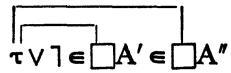
\includegraphics[keepaspectratio]{images/part001_434fa5c1de2e0e5711bd2657d8ea90475ca0e52e33fa2d57a405da317d612ec5.jpg}}

就是一个组装。*

完全使用组装将给印刷者和读者都带来难以克服的困难。因此，现行文本使用不属于形式数学的缩写符号（尤其是日常语言中的词语）。引入此类符号是定义的目的。它们的使用对理论并非必不可少，且常常可能导致混淆，只有读者对主题具备一定熟悉程度才能避免。

\minorheading{示例}

\begin{enumerate}
\def\labelenumi{(\arabic{enumi})}
\item
  组装 \(\vee\neg\) 用 \(\Longrightarrow\) 表示。
\item
  以下符号表示组装（而且是非常长的组装）：
\end{enumerate}

\[
\begin{gathered}
\text{``3 且 4''} \\
\phi \\
\mathbf{N} \\
\mathbf{Z} \\
\text{``实数直线''} \\
\text{``该 }\Gamma\text{ 函数''} \\
f \circ g \\
\pi = \sqrt{2} + \sqrt{3} \\
1 \in 2
\end{gathered}
\]

“每个有限除环都是域”

“\(\zeta(s)\) 的零点，除 \(-2, -4, -6, \ldots\) 之外，位于直线上

\[
\mathcal{R}(s) = 1/2
\]''.

一般来说，用来表示一个组装的符号包含该组装中出现的所有字母。不过，有时也可以违反这一原则而不致混淆。*例如，“X的完备化”表示一个含有字母X的组装，同时还含有另一个字母，用来表示X的一致结构的周围集族。另一方面，

\[
\int_ {0} ^ {1} f (x) d x
\]

表示一个不含字母x（也不含字母d）的组装；N、Z和“Γ函数”所表示的组装也不含任何字母。*

一个数学理论（或简称理论）包含一些规则，这些规则允许我们断言某些符号组合是该理论的项或关系，以及其他规则允许我们断言某些组合是该理论的定理。

本章中对这些规则的描述并不属于形式数学的范畴；这些规则涉及或多或少未确定的组合，例如未确定的字母。为简化表述，我们便于用较不繁琐的符号来指称此类组合。我们将特别使用（数学理论的）符号组合、粗斜体字母（带或不带下标或重音符号）以及特定符号，其中将给出一些示例。由于我们的目的仅在于避免迂回说法（参见§3第1号第28页脚注(*)），我们不会为这些符号的使用制定严格的一般规则；读者在每种具体情况下都能毫无困难地重构所涉及的组合。为用语简便，我们常称这些符号即为组合，而非它们表示组合；因此，在以下规则的陈述中，诸如“组合A”或“字母x”之类的表述，应替换为“由A表示的组合”或“由x表示的字母”。

设 \(A\) 和 \(B\) 为组装。用 \(AB\) 表示把组装 \(B\) 写在组装 \(A\) 右边所得的组装。用 \(\vee A \neg B\) 表示从左到右依次写下符号 \(\vee\) 、组装 \(A\) 、符号 \(\neg\) 和组装 \(B\) 所得的组装。其余类推。

设 \(A\) 为一个组装，\(x\) 为一个字母。用 \(\tau_{x}(A)\) 表示按如下方式构造的组装：先形成组装 \(\tau A\) ，把 \(x\) 在 \(A\) 中的每一处出现与 \(\tau\) 相连，后者写在 \(A\) 左侧；再把每一处 \(x\) 都换成符号 \(\square\) 。因此，\(\tau_{x}(A)\) 所表示的组装不含 \(x\) 。

例。符号 \(\tau_{x}(\in xy)\) 表示组装

\[
\tau \in \square y.
\]

设A和B为组装，x为一个字母。将A中所有出现的x替换为组装B所得的组装记为 \((B|x)A\) （读作：B 在 A 中替换 x）。如果 x 不出现在 A 中，则 \((B|x)A\) 与 A 相同；特别地，

\[
(B | \boldsymbol {x}) \tau_ {\boldsymbol {x}} (A)
\]

与 \(\tau_{\mathbf{x}}(A)\) 相同。

例。若将 \(x\) 替换为 \(\square\) ，每逢 \(x\) 在组装 \(\vee \in xy = xx\) 中出现便作此替换，就得到组装 \(\vee \in \square y = \square \square\) 。

若 \(A\) 是一个组装，而我们特别关注一个字母 \(x\) ，或两个不同的字母 \(x\) 和 \(y\) （它们可以出现或不出现在 \(A\) 中），则常写作 \(A \{x\}\) 或 \(A \{x, y\}\) 。在这种情况下，用 \(A \{B\}\) 代替 \((B|x)A\) 。用 \(A \{B, C\}\) 表示同时把 \(x\) 换成 \(B\) 、把 \(y\) 换成 \(C\) （每逢它们在 \(A\) 中出现便作替换；注意，\(x\) 和 \(y\) 可以出现在 \(B\) 及 \(C\) 中）；若 \(x'\) 和 \(y'\) 是不同于 \(x\) 和 \(y\) 的两个不同字母，并且均不出现在 \(A, B\) 或 \(C\) 中，则 \(A \{B, C\}\) 与 \((B|x') (C|y') (x'|x) (y'|y)A\) 相同。

备注。当引入一个缩写符号 \(\Sigma\) （借助定义）用以表示某个组装时，通常（隐含地）约定：将原组装中的字母x替换为组装B所得到的组装，用将 \(\Sigma\) 中的字母x替换为组装B（或更常见地，替换为表示组装B的缩写符号）后所得的符号来表示。

¶ *例如，一旦定义了由符号E⊗F所表示的组装——其中E和F是字母，这个组装此外还包含除E和F之外的其他字母——符号Z⊗F就可以无需进一步解释地使用。*

¶ 这条规则可能会导致混淆，而通过使用各种排版手段可以避免这些混淆；最常见的方法是用 (B) 替换 x 来代替 B。

¶ *例如，M∩N 表示一个包含字母 N 的组装。如果我们用 P∪Q 所表示的组装替换 N，则得到由 M∩(P∪Q) 表示的组装。*

\subsection{替换的准则}

形式数学仅包含明确书写的组装。然而，即使使用缩写符号，严格依照此原则发展数学也会导致极其冗长的推理链条。因此，我们将建立与不定组装相关的准则；每条准则将一次性描述对这些组装进行特定操作序列的最终结果。这些准则因此并非理论所必需；其合理性属于元数学范畴。

元数学本身的发展，在实践中需要使用一些缩写符号，其中部分符号已在前面提及。这些符号中的大多数在数学中也有使用。

我们将使用以下准则，称为代入准则：

CS1. 设A和B为组装，x和 \(x'\) 为字母。若 \(x'\) 不出现在 A 中，则 \((B|x)A\) 与 \((B|x')(x'|x)A\) 相同。

CS2. 设 \(A, B\) 和 \(C\) 为组装，\(x\) 和 \(y\) 为不同的字母\footnote{按照第 1 号所述，“x 和 y 是不同的字母”这一说法是一种语言上的滥用：它表示在所考虑的组装中，x 和 y 表示不同的字母。}。若 \(y\) 不出现在 \(B\) 中，则 \((B|x)(C|y)A\) 与下式相同：

\[
\left(\boldsymbol {C} ^ {\prime} | \boldsymbol {y}\right) (\boldsymbol {B} | \boldsymbol {x}) \boldsymbol {A},
\]

其中 \(C'\) 是组装 \((B|x)C\) 。

CS3. 设 A 为一个组装，x 和 \(x'\) 为字母。若 \(x'\) 不出现在 A 中，则 \(\tau_{\mathbf{x}}(A)\) 与 \(\tau_{\mathbf{x}'}(A')\) 相同，其中 \(A'\) 是组装 \((x'|x)A\) 。

CS4. 设 A 和 B 为组装，x 和 y 为不同的字母。若 x 不出现在 B 中，则 \((B|y)\tau_{x}A\) 与 \(\tau_{x}(A')\) 相同，其中 \(A'\) 是组装 \((B|y)A\) 。

CS5. 设 \(A, B, C\) 为组装，\(x\) 为一个字母。组装 \((C|x) (\neg A), (C|x) (\vee AB), (C|x) (\Longrightarrow AB), (C|x) (sAB)\) （其中 \(s\) 是一个特定符号）分别与 \(\neg A', \vee A'B', \Longrightarrow A'B', sA'B',\) 相同，其中 \(A', B'\) 分别是 \((C|x) A, (C|x) B\) 。

下面以CS2为例说明验证的原理。比较把A变为 \((B|x)(C|y)A\) 的操作与把A变为 \((C'|y)(B|x)A\) 的操作。在这两种操作中，A内不同于x和y的符号都不改变。在A中每一处x出现的位置，两种操作都以B替换x；对于第一种操作这是显然的，对于第二种操作则由y不出现在B中而知。最后，在A中每一处y出现的位置，第一种操作先以C替换y，再在C中每一处x出现的位置以B替换x；这显然等同于在A中每逢y出现便以组装 \((B|x)C\) 替换。

\subsection{形成性构造}

一个理论的一些特定符号被称为关系性的，而其他的被称为实体性的。每个特定符号都关联一个自然数，称为其权重（实际上通常为2）。

¶ 如果一个组装以τ开头，或以实体符号开头，或者仅由一个字母组成，则称其为第一类组装；否则为第二类组装。

¶ 理论 \(\mathfrak{C}\) 中的一个形成性构造，是满足如下性质的组装序列：序列中的每个组装 A 都满足以下条件之一：

\begin{enumerate}
\def\labelenumi{(\alph{enumi})}
\item
  A 是一个字母。
\item
  在序列中存在一个第二类的组装 B，位于 A 之前，使得 A 是 \(\neg B\) .
\item
  存在两个组装 \(\pmb{B}\) 并且 \(\pmb{C}\) （第二类，相同或不同），位于 \(\pmb{A}\) 之前，使得 \(\pmb{A}\) 是 \(\vee \pmb{BC}\) .
\item
  存在一个第二类的组装 B，位于 A 之前，以及一个字母 x，使得 A 是 \(\tau_{x}(B)\) .
\item
  有一个特定符号 \(s\) ，其权重为 \(n\)\footnote{如上所述，为了发展当今的数学理论，可以将我们的考虑限于权重为 2 的特定符号，从而避免在形成性构造的定义中使用“自然数 n”这一表述。} ，并且属于 \(\mathfrak{C}\) ；还有 \(n\) 个第一类组装 \(A_{1}, A_{2}, \ldots, A_{n}\) ，它们先于 \(A\) 出现，使得 \(A\) 是 \(sA_{1}A_{2} \ldots A_{n}\) 。
\end{enumerate}

¶ 出现在 \(\mathfrak{C}\) 的形成性构造中的第一类（相应地，第二类）组装，称为 \(\mathfrak{C}\) 中的项（相应地，关系）。

示例。*在集合论中，其中 \(\in\) 是权重为2的关系符号，以下组装序列是一个形成性构造：

\pandocbounded{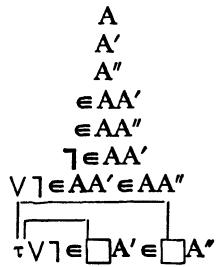
\includegraphics[keepaspectratio]{images/part001_f4a426ee2f8fe397dc0bc6599464a758ff3a832b6925cc474c9242d7de093d2f.jpg}}

因此，第1号示例中给出的组装是集合论中的一个项。*

备注。直观地说，项是表示对象的组装，而关系是表示关于这些对象可以作出的断言的组装。条件（a）意味着字母表示对象。条件（b）意味着如果B是一个断言，那么 \(\neg B\) 称为B的否定，是一个命题（读作：非B）。条件(c)意味着如果B和C是命题， \(\vee BC\) 称为B和C的析取，是一个命题（读作：B或C）；因此 \(\Longrightarrow BC\) 是一个命题（用语言表述为：“非B，或C”，或“B蕴含C”）。条件(d)意味着如果B是一个命题且x是一个字母，那么 \(\tau_{X}(B)\) 是一个对象。让我们将命题B视为表达对象X的一个性质；那么，如果存在一个具有该性质的对象， \(\tau_{X}(B)\) 表示一个具有此性质的特定对象；如果没有， \(\tau_{X}(B)\) 表示一个关于它无法言说的对象。最后，条件(e)意味着如果 \(A_{1}, A_{2}, ..., A_{n}\) 是对象，且s是一个n元关系（或实体）符号，那么 \(sA_{1}A_{2}\ldots A_{n}\) 是关于对象 \(A_{1}, ..., A_{n}\) 的一个命题（相应地，一个依赖于 \(A_{1}, ..., A_{n}\) 的对象).

示例。符号 \(\phi\) , \(\mathbf{N}\) “实数直线”，“该 \(\Gamma\) 函数”， \(f \circ g\) 表示项。符号 \(\pi = \sqrt{2} + \sqrt{3}\) , \(1 \in 2\) ，“每个有限除环都是域”，“\(\zeta(s)\) 的除 \(-2, -4, -6, \ldots\) 之外的零点位于直线上 \(\mathcal{R}(s) = 1/2\)'' 表示关系。符号“3和4”既不表示项，也不表示关系。

关系的初始符号是 \(\vee, \neg\) ，或关系符号。项的初始符号要么是 \(\tau\) 或一个实体性的符号，前提是该项并非由单个字母组成。后一断言源于这样一个事实：项是第一类组装。如果 \(A\) 是一个关系，则 \(A\) 出现在一个形成性构造中，不是字母，且不以 \(\tau\) 开头，因此可能存在三种情况：（1） \(A\) 前面有一个组装 \(B\) 使得 \(A\) 是 \(\neg B\) ; (2) \(A\) 前面有两个组装 \(B\) 和 \(C\) 使得 \(A\) 是 \(\vee BC\) ; (3) \(A\) 前面有组装 \(A_1, A_2, ..., A_n\) 使得 \(A\) 是 \(sA_1A_2 ... A_n\) , \(s\) 作为一个关系符号。

\subsection{形成性判据}

CF1. 如果 \(A\) 和 \(B\) 是理论 \(\mathfrak{G}\) 中的关系，那么 \(\vee AB\) 是 \(\mathfrak{G}\) 中的关系。

考虑 \(\mathfrak{G}\) 中的两个形成性构造，其中一个包含 \(A\) ，另一个包含 \(B\) 。依次写出第一个构造的组装、第二个构造的组装，最后写出 \(\vee AB\) ，便得到一个组装序列。由于 \(A\) 和 \(B\) 都属于第二类，立即可以验证这个序列是 \(\mathfrak{G}\) 中的形成性构造。组装 \(\vee AB\) 属于第二类，因此它是 \(\mathfrak{G}\)

中的一个关系。以下三个判据可用类似方法建立：

CF2. 若A是理论C中的一个关系，则 \(\neg A\) 是 C 中的一个关系。

CF3. 若A是理论G中的一个关系，且x是一个字母，则 \(\tau_{x}(A)\) 是 G 中的一个项。

CF4. 如果 \(A_1, A_2, \ldots, A_n\) 是理论 \(\mathfrak{C}\) 中的项，并且 \(s\) 是权重为 \(n\) 的关系符号（相应地，实体符号），且属于 \(\mathfrak{C}\) ，那么 \(sA_1A_2\ldots A_n\) 是 \(\mathfrak{C}\) 中的关系（相应地，项）。

这些准则立即蕴含以下结论：

如果A和B是理论C中的关系，那么 \(\Longrightarrow AB\) 是 C 中的一个关系。

CF6。设 \(A_1, A_2, \ldots, A_n\) 是理论 \(\mathfrak{C}\) 中的一个形成性构造，\(x\) 和 \(y\) 是字母。假设 \(y\) 不出现在任何 \(A_i\) 中。那么 \((y|x)A_1\) , \((y|x)A_2, \ldots, (y|x)A_n\) 是 \(\mathfrak{C}\)

中的一个形成性构造。为证明CF6，令 \(A_i'\) 为组装 \((y|x)A_i\) 。如果 \(A_i\) 是一个字母，则 \(A_i'\) 也是一个字母。如果 \(A_i\) 具有形式 \(\neg A_j\) ，其中 \(A_j\) 是在构造中先于 \(A_i\) 的第二类组装，则由CS5，\(A_i'\) 与 \(\neg A_j'\) 相同，而 \(A_j'\) 是第二类组装。若 \(A_i\) 具有形式 \(\vee A_jA_k\) 或 \(sA_{j_1}A_{j_2}\ldots A_{j_m}\) ，其中 \(s\) 是 \(\mathfrak{G}\) 的特定符号，论证类似。最后，若 \(A_i\) 具有形式 \(\tau_z(A_j)\) ，其中 \(A_j\) 是在构造中先于 \(A_i\) 的第二类组装，则需考虑以下几种情形：

\begin{enumerate}
\def\labelenumi{(\alph{enumi})}
\item
  z 是一个与 x 和 y 不同的字母。那么 \(A_{i}^{\prime}\) 与 \(\tau_{z}(A_{j}^{\prime})\) 相同，根据 CS4，且 \(A_{j}^{\prime}\) 是第二类的组装。
\item
  z 与 x 相同。那么 \(A_{i}\) 不包含 x，因此 \(A_{i}^{\prime}\) 与 \(A_{i}\) 相同，也就是说与 \(\tau_{x}(A_{j})\) 相同；由于 y 不出现在 \(A_{j}\) 中，\(\tau_{x}(A_{j})\) 与 \(\tau_{y}(A_{j})\) 相同，根据 CS3。
\item
  z 与 y 相同。那么 \(A_{i}\) 是组装 \(\tau A_{j}\) ，因为 y 不出现在 \(A_{j}\) 中；因此 \(A_{i}^{\prime}\) 是组装 \(\tau A_{j}^{\prime}\) ，即 \(\tau_{u}(A_{j}^{\prime})\) ，其中 u 是一个不出现在 \(A_{j}^{\prime}\) 中的字母。
\end{enumerate}

CF7. 设 \(A\) 为理论 \(\mathfrak{G}\) 中的一个关系（相应地，一个项），\(x\) 和 \(y\) 为字母。那么 \((y|x)A\) 是 \(\mathfrak{G}\) 中的一个关系（相应地，一个项）。

设 \(A_1, A_2, \ldots, A_n\) 是一个形成性构造，其中 \(A\) 出现。我们将逐步证明，如果 \(A_t\) 是一个关系（相应地，一个项）则 \((y|x)A_t\) ，我们将其记为 \(A_t'\) ，也是一个关系（相应地，一个项）。假设这一点已经对 \(A_1, A_2, \ldots, A_{i-1}\) 成立；让我们对 \(A_i\) 加以证明。如果 \(A_i\) 是一个字母，则 \(A_i'\) 是一个字母。如果 \(A_i\) 在构造中先于一个关系 \(A_j\) 使得 \(A_i\) 是 \(\neg A_j\) ，那么 \(A_i'\) 与 \(\neg A_j'\) 相同（由CS5），且 \(\neg A_j'\) 是由CF2得到的一个关系。论证类似，如果 \(A_i\) 前面有关系 \(A_j, A_k\) 使得 \(A_i\) 是 \(\vee A_jA_k\) ，或者如果 \(A_i\) 前面有项 \(A_{j_1}, \ldots, A_{j_m}\) 使得 \(A_i\) 是 \(sA_{j_1}\ldots A_{j_m}\) ，其中 \(s\) 是 \(\mathfrak{G}\) 的一个权重为 \(m\) 的特定符号。最后，如果 \(A_i\) 前面有一个关系 \(A_j\) 使得 \(A_i\) 是 \(\tau_z(A_j)\) ，则有各种情况需要考虑：

\begin{enumerate}
\def\labelenumi{(\alph{enumi})}
\item
  z 与 x 和 y 均不同。那么 \(A_{i}^{\prime}\) 与 \(\tau_{\mathbf{z}}(A_{j}^{\prime})\) 相同，由CS4可知，并且我们已经知道 \(A_{j}^{\prime}\) 是一个关系；因此 \(A_{i}^{\prime}\) 根据 CF3 是一个项。
\item
  \(z\) 与 \(x\) 相同。然后 \(A_i\) 不包含 \(x\) ，因此 \(A_i'\) 与 \(A_i\) 相同，从而是一个项。
\item
  \(z\) 与 \(y\) 相同。然后令 \(u\) 为一个字母，与 \(x\) 和 \(y\) 均不同，且不出现在 \(A_1, A_2, \ldots, A_j\) 中。根据CF6，组装序列 \((u|y) A_1, \ldots, (u|y) A_j\) ，我们将其记为 \(A_1'', \ldots, A_j''\) ，构成了 \(\mathfrak{G}\) 中的一个形成性构造。由于 \(y\) 不再出现在这个新构造中，\((y|x) A_1'', \ldots, (y|x) A_j''\) 根据CF6是一个形成性构造，因此 \((y|x) A_j''\) 是 \(\mathfrak{G}\) 中的一个关系；因此 \(\tau_u((y|x)A_j'')\)
\end{enumerate}

是 \(\mathfrak{C}\) 中的一个项。但由CS4，这个项与 \((y|x)\tau_u(A_j'')\) 相同；再由CS3，它与 \((y|x)\tau_y(A_j)\) 相同，因而与 \(A_i'\) 相同。

CF8. 设 \(A\) 为理论 \(\mathfrak{G}\) 中的一个关系（相应地，一个项），\(x\) 为一个字母，\(T\) 为 \(\mathfrak{G}\) 中的一个项。那么 \((T|x)A\) 是 \(\mathfrak{G}\) 中的一个关系（相应地，一个项）。

设 \(A_1, A_2, \ldots, A_n\) 是一个形成性构造，其中 \(A\) 出现。设 \(x_1, x_2, \ldots, x_p\) 为出现在 \(T\) 中的不同字母。让我们将每个字母 \(x_i\) 与一个字母 \(x_i'\) 相关联，后者与每个字母 \(x_1, \ldots, x_p\) 以及出现在 \(A_1, \ldots, A_n\) 中的字母均不同，且使得字母 \(x_1', \ldots, x_p'\) 两两互异。该组装

\[
\left(\boldsymbol {x} _ {1} ^ {\prime} \mid \boldsymbol {x} _ {1}\right) \left(\boldsymbol {x} _ {2} ^ {\prime} \mid \boldsymbol {x} _ {2}\right) \dots \left(\boldsymbol {x} _ {p} ^ {\prime} \mid \boldsymbol {x} _ {p}\right) \boldsymbol {T}
\]

是一个项 \(\pmb{T}'\) ，依据CF7，且 \((\pmb{T}|\pmb{x})\pmb{A}\) 与

\[
\left(\boldsymbol {x} _ {1} \mid \boldsymbol {x} _ {1} ^ {\prime}\right) \left(\boldsymbol {x} _ {2} \mid \boldsymbol {x} _ {2} ^ {\prime}\right) \dots \left(\boldsymbol {x} _ {p} \mid \boldsymbol {x} _ {p} ^ {\prime}\right) \left(\boldsymbol {T} ^ {\prime} \mid \boldsymbol {x}\right) \boldsymbol {A}
\]

相同，这通过应用CS1得到。因此只需证明 \((T^{\prime}|x)A\) 是一个关系（相应地，一个项）；换言之，从现在起我们可以假设出现在 \(T\) 中的字母不出现在 \(A_{1},\ldots ,A_{n}\) 中。我们将逐步证明，如果 \(A_{t}\) 是一个关系（相应地，一个项），则 \((T|x)A_{t}\) ，我们将其记为 \(A_{t}^{\prime}\) ，是一个关系（相应地，一个项）。假设这一点已对 \(A_{1},A_{2},\ldots ,A_{i - 1}\) 成立，并让我们证明它对于 \(A_{i}\) 。如果 \(A_{i}\) 是一个字母，则 \(A_{i}^{\prime}\) 要么是同一个字母，要么是 \(T\) ，因此是一个项。如果 \(A_{i}\) 具有形式 \(\lnot A_j\) ，其中 \(A_{j}\) 是一个在构造中先于 \(A_{i}\) 的关系，那么 \(A_{i}^{\prime}\) 与 \(\lnot A_j^{\prime}\) 相同，根据CS5，并且我们已经知道 \(A_{j}^{\prime}\) 是一个关系，因此 \(A_{i}^{\prime}\) 根据CF2是一个关系。如果 \(A_{i}\) 具有形式 \(\vee A_{j}A_{k}\) ，或 \(sA_{j_1}\ldots A_{j_m}\) ，证明是类似的。最后，如果 \(A_{i}\) 具有形式 \(\tau_{z}(A_j)\) ，其中 \(A_{j}\) 是一个在构造中先于 \(A_{i}\) 的关系，则有各种情况需要考虑：

\begin{enumerate}
\def\labelenumi{(\alph{enumi})}
\item
  \(z\) 与 \(x\) 以及出现在 \(T\) 中的字母均不同。然后 \(A_i'\) 与 \(\tau_z(A_j')\) 相同，由CS4可知，并且我们已经知道 \(A_j'\) 是一个关系；因此 \(A_i'\) 根据CF3是一个项。
\item
  \(\pmb{z}\) 与 \(\pmb{x}\) 相同。然后 \(A_{i}\) 不包含 \(\pmb{x}\) ，因此 \(A_{i}'\) 与 \(A_{i}\) 相同，因此是一个项。
\item
  \(z\) 出现在 \(T\) 。然后 \(z\) 不出现在 \(A_j\) 中，因此 \(A_i'\) 与 \(\tau A_j\) 相同；因此 \(A_i'\) 与 \(\tau A_j'\) 相同。现在，我们已经知道 \(A_j'\) 是一个关系，而 \(\tau A_j'\) 与 \(\tau_u(A_j')\) 相同，其中 \(u\) 是一个不出现在 \(A_j'\) 中的字母；根据CF3可知， \(A_i'\) 是一个项。
\end{enumerate}

直观地说，如果A是C中的一个关系，我们可以将其视为表达对象x的某种性质，那么断言 \((B|x)A\) 相当于说对象B具有这一性质。如果A是C中的一个项，它表示一个以某种方式依赖于由x所表示的对象；项 \((B|x)A\) 表示当我们把x取为对象B时，对象A所变成的东西。

\section{定理}

从现在起，如果 \(A\) 是一个关系，我们将用 not(A) 代替 \(\neg A\) 。如果 \(A\) 和 \(B\) 是关系，我们将写“(A) 或 (B)”代替 \(\vee AB\) ，以及 \((A) \Longrightarrow (B)\) 代替 \(\Longrightarrow AB\) 。有时我们会省略括号。在每种情况下，读者都能毫不困难地确定所考虑的组装。

\subsection{公理}

我们已经看到，特定符号决定了理论 \(\mathfrak{G}\) 中的项和关系。为了构造 \(\mathfrak{G}\) ，我们按以下步骤进行：

\begin{enumerate}
\def\labelenumi{(\arabic{enumi})}
\item
  首先我们在 \(\mathfrak{G}\) 中写下一定数量的关系；这些关系称为 \(\mathfrak{G}\) 的显式公理。出现在显式公理中的字母称为 \(\mathfrak{G}\) 的常量.
\item
  我们规定一条或多条规则\footnote{为简洁起见，这些规则使用§1第1号中提到的符号（尤其是粗斜体字母）来表达；但在规则的表述中完全避免使用这些符号也是容易做到的（见§3第1号，第28页脚注(*)）。}，称为 \(\mathfrak{C}\) 的方案，它们必须具有以下性质：（a）应用这样的规则 \(\mathcal{R}\) 给出 \(\mathfrak{C}\) 中的一个关系； (b) 如果 \(T\) 是 \(\mathfrak{C}\) 中的一项，如果 \(x\) 是一个字母，且如果 \(R\) 是 \(\mathfrak{C}\) 中的一个关系（由方案 \(\mathcal{R}\) 构造），则关系 \((T|x)R\) 也可以通过应用 \(\mathcal{R}\) 得到。
\end{enumerate}

在我们设想的所有情形中，这些条件的验证总是容易的。

通过应用 \(\mathfrak{G}\) 的某个方案构造的每个关系，称为 \(\mathfrak{G}\) 的隐式公理。

直观上，公理要么表示自明的主张，要么表示人们希望从中推出结论的假设。常量表示已明确定义的对象，显式公理所表达的性质被认为对这些对象成立。另一方面，如果字母 x 不是常量，则它表示一个完全未确定的对象；如果通过公理假定对象 x 具有某种性质，则该公理必然是隐式的，因此该性质对任何对象 T 仍然成立。

\subsection{证明}

\(\mathfrak{G}\) 中的一个示范性文本包括：

\begin{enumerate}
\def\labelenumi{(\arabic{enumi})}
\item
  \(\mathfrak{G}\) 中关系与项的一个辅助形成性构造 .
\item
  \(\mathfrak{G}\) 中的一个证明，即 \(\mathfrak{G}\) 中的一个关系序列，这些关系都出现在辅助形成性构造中，使得对于序列中的每一个关系 \(\pmb{R}\) ，至少满足以下条件之一：
\end{enumerate}

\((a_{1})\boldsymbol{R}\) 是 \(\mathfrak{c}\) 的一条显式公理 .

\((a_{2})\) R 是由将 C 的一个方案应用于辅助形成性构造中出现的项或关系而得出的结果。

\begin{enumerate}
\def\labelenumi{(\alph{enumi})}
\setcounter{enumi}{1}
\tightlist
\item
  有两个关系 \(S, T\) 在序列中位于 \(R\) 之前，使得 \(T\) 是 \(S \Longrightarrow R\) .
\end{enumerate}

¶ \(\mathfrak{G}\) 中的一个定理，是在 \(\mathfrak{G}\) 的一个证明中出现的关系。

因此，这一概念本质上依赖于所考虑理论在被描述时的状态。理论 \(\mathfrak{G}\) 中的一个关系，当人们成功地将它插入到 \(\mathfrak{G}\) 的一个证明中时，便成为 \(\mathfrak{G}\) 中的一条定理。要说 \(\mathfrak{G}\) 中的一个关系``不是 \(\mathfrak{G}\) 中的定理''，若不参照理论 \(\mathfrak{G}\) 的发展阶段，便不具有任何意义。

\(\mathfrak{G}\) 中的定理也被称为“\(\mathfrak{G}\) 中的真关系”（或“命题”、“引理”、“推论”等）。设 \(R\) 是 \(\mathfrak{G}\) 中的一个关系，设 \(x\) 是一个字母，\(T\) 是 \(\mathfrak{G}\) 中的一个项；若 \((T|x)R\) 是 \(\mathfrak{G}\) 中的定理，则称 \(T\) 满足关系 \(R\) （在 \(\mathfrak{G}\) 中；或称为 \(R\) 的解），这里 \(R\) 被视为 \(x\) 中的关系。

一个关系，若其否定是 \(\mathfrak{c}\) 中的定理，则被称为在 \(\mathfrak{c}\) 中是假的。一个理论 \(\mathfrak{c}\) ，当其中写有一个在 \(\mathfrak{c}\) 中既真又假的关系时，就被称为矛盾的。

这里我们再次涉及一个依赖于理论特定发展状态的概念。读者应当警惕一种混淆（不幸的是，这种混淆由“假”一词的直观含义所暗示），即认为一旦证明了关系 R 在 \(\mathfrak{G}\) 中为假，就由此确立了 R 在 \(\mathfrak{G}\) 中“不真”（严格来说，正如我们上面所指出的，这个短语在数学中没有精确的含义）。

¶ 在下文中，我们将给出称为演绎准则的元数学准则，它们将使我们能够缩短证明。这些准则将用字母 C 后跟一个数字来表示。

C1（三段论）。设 A 和 B 是理论 C 中的关系。如果 A 和 \(A \Longrightarrow B\) 是 C 中的定理，则 B 是 C 中的定理。

设 \(R_1, R_2, \ldots, R_n\) 是 \(\mathfrak{G}\) 中的一个证明，在其中 \(A\) 出现，并且令 \(S_1, S_2, \ldots, S_p\) 是 \(\mathfrak{G}\) 中的一个证明，在其中 \(A \Longrightarrow B\) 出现。显然 \(R_1, R_2, \ldots, R_n, S_1, S_2, \ldots, S_p\) 是 \(\mathfrak{G}\) 中的一个证明，在其中 \(A\) 和 \(A \Longrightarrow B\) 都出现。因此

\[
\boldsymbol {R} _ {1}, \boldsymbol {R} _ {2}, \dots , \boldsymbol {R} _ {n}, \boldsymbol {S} _ {1}, \boldsymbol {S} _ {2}, \dots , \boldsymbol {S} _ {p}, \boldsymbol {B}
\]

是 \(\mathfrak{c}\) 中的一个证明，从而 \(\pmb{B}\) 是 \(\mathfrak{c}\) 中的定理 .

\subsection{理论中的代入}

设 \(\mathfrak{c}\) 为一个理论，令 \(A_{1}, A_{2}, \ldots, A_{n}\) 为其显式公理，令 \(\pmb{x}\) 为一个字母，并且令 \(\pmb{T}\) 为 \(\mathfrak{c}\) 的一项。设 \((\pmb{T}|\pmb{x})\mathfrak{c}\) 为这样的理论，其符号和方案与 \(\mathfrak{c}\) 的相同，且其显式公理为 \((\pmb{T}|\pmb{x})\pmb{A}_{1}, (\pmb{T}|\pmb{x})\pmb{A}_{2}, \ldots, (\pmb{T}|\pmb{x})\pmb{A}_{n}\) .

C2。设A是理论 \(\mathfrak{G}\) 中的一个定理，设T是 \(\mathfrak{G}\) 的一个项，并设x是一个字母。则 \((T|x)A\) 是理论 \((T|x)\mathfrak{G}\) 中的定理。

设 \(R_1, R_2, \ldots, R_n\) 是 \(\mathfrak{G}\) 中的一个证明，在其中 \(A\) 出现。考虑序列 \((T|x)R_1, (T|x)R_2, \ldots, (T|x)R_n\) ，这是 \(\mathfrak{G}\) 中的关系序列，依据是CF8（§1，第4号）。我们将证明这个序列是该理论 \((T|x)\mathfrak{G}\) 中的一个证明；这将确立该准则。如果 \(R_k\) 是 \(\mathfrak{G}\) 的一个隐式公理，那么 \((T|x)R_k\) 同样是 \(\mathfrak{G}\) 的一个隐式公理（编号1），因此也是 \((T/x)\mathfrak{G}\) 的。如果 \(R_k\) 是 \(\mathfrak{G}\) 的一条显式公理，那么 \((T|x)R_k\) 是 \((T|x)\mathfrak{G}\) 的一条显式公理。最后，如果 \(R_k\) 前面有关系 \(R_i\) 和 \(R_j\) ，其中 \(R_j\) 是 \(R_i \Longrightarrow R_k\) ，那么 \((T|x)R_k\) 前面是 \((T|x)R_i\) 和 \((T|x)R_j\) ，后者与 \((T|x)R_i \Longrightarrow (T|x)R_k\) （准则CS5）相同。

C3. 设 A 是理论 G 的一个定理，设 T 是 G 的一个项，并设 x 是一个不是 G 的常量的字母。则 \((T|x)A\) 是 G 的一个定理。

这直接从 C2 推出，因为 x 不出现在 \(\mathfrak{G}\)的显式公理中。更特别地，如果 \(\mathfrak{G}\) 不包含任何显式公理，或者显式公理中不包含任何字母，那么准则C3对字母x的应用不受限制。

\subsection{理论的比较}

一个理论 \(\mathcal{C}'\) 被认为强于理论 \(\mathcal{C}\) ，如果 \(\mathcal{C}\) 的所有符号都是 \(\mathcal{C}'\) 的符号， \(\mathcal{C}\) 的所有显式公理都是 \(\mathcal{C}'\) 中的定理，以及 \(\mathcal{C}\) 的方案是 \(\mathcal{C}'\) 的方案。

C4. 如果理论 \(\mathfrak{G}'\) 强于理论 \(\mathfrak{G}\) ，那么 \(\mathfrak{G}\) 的所有定理都是 \(\mathfrak{G}'\) .

设 \(R_1, R_2, \ldots, R_n\) 是 \(\mathfrak{G}\) 中的一个证明。我们将逐步证明，每一个 \(R_i\) 是 \(\mathfrak{G}'\) 中的定理 。假设这一点对先于 \(R_k\) 的关系成立。如果 \(R_k\) 是 \(\mathfrak{G}\) 的公理，则它是 \(\mathfrak{G}'\) 中的一个定理，根据假设。如果 \(R_k\) 前面有关系 \(R_i\) 和 \(R_i \Longrightarrow R_k\) ，我们已经知道 \(R_i\) 和 \(R_i \Longrightarrow R_k\) 是 \(\mathfrak{G}'\) 中的定理，从而 \(R_k\) 是 \(\mathfrak{G}'\) 中的定理 ，根据C1。因此，在每种情况下， \(R_k\) 是 \(\mathfrak{G}'\) 中的定理 ，证明完成。

如果两个理论 \(\mathfrak{G}\) 和 \(\mathfrak{G}'\) 中的每一个都比另一个更强， \(\mathfrak{G}\) 和 \(\mathfrak{G}'\) 被称为等价的。那么 \(\mathfrak{G}\) 的每一个定理都是 \(\mathfrak{G}'\) 中的一个定理，反之亦然。

C5. 设 \(\mathfrak{G}\) 设为一个理论，令 \(A_{1}, A_{2}, \ldots, A_{n}\) 为其显式公理， \(a_{1}, a_{2}, \ldots, a_{h}\) 其常量，并令 \(T_{1}, T_{2}, \ldots, T_{h}\) 为 \(\mathfrak{G}\) 中的项。假设

\[
\left(\boldsymbol {T} _ {1} \mid \boldsymbol {a} _ {1}\right) \left(\boldsymbol {T} _ {2} \mid \boldsymbol {a} _ {2}\right) \dots \left(\boldsymbol {T} _ {h} \mid \boldsymbol {a} _ {h}\right) \boldsymbol {A} _ {i} \quad (\text { 对 } i = 1, 2, \dots , n)
\]

是某个理论 \(\mathfrak{G}'\) 中的定理，并且 \(\mathfrak{G}\) 的所有符号都是 \(\mathfrak{G}'\) 的符号，并且 \(\mathfrak{G}\) 的方案是 \(\mathfrak{G}'\) 的方案。那么，若 \(A\) 是 \(\mathfrak{G}\) 中的定理 ,

\[
\left(\boldsymbol {T} _ {1} \mid \boldsymbol {a} _ {1}\right) \dots \left(\boldsymbol {T} _ {h} \mid \boldsymbol {a} _ {h}\right) \boldsymbol {A}
\]

是 \(\mathfrak{C}'\) 中的定理 .

因为 \(\mathfrak{c}'\) 比理论 \((T_1|a_1) \ldots (T_h|a_h)\mathfrak{c}\) 更强，所以可以应用C2和C4。

当我们使用这一程序来从 \(\mathfrak{C}\) 的一个定理推导 \(\mathfrak{C}'\) 中的一个定理时，我们说我们在 \(\mathfrak{C}'\) 中应用 \(\mathfrak{C}\) 的结果。直观上，公理 \(\mathfrak{C}\) 表达了 \(a_1, a_2, \ldots, a_h\) 的一些性质，而 \(A\) 表达了由这些公理推出的一个性质。如果这些对象 \(T_1, T_2, \ldots, T_h\) 在 \(\mathfrak{C}'\) 中具有由公理 \(\mathfrak{C}\) 所表达的性质，那么它们也具有性质 \(A\) .

*例如，在群论 \(\mathfrak{C}\) 中，显式公理包含两个常量 \(G\) 和 \(\mu\) （群和合成法则）。在集合论 \(\mathfrak{C}'\) 中，我们定义两个项：实数直线和实数加法。如果我们将这些项分别代入 \(G\) 和 \(\mu\) ，也就是在 \(\mathfrak{C}\) 的显式公理中作此代入，我们就在 \(\mathfrak{C}'\) 中得到定理。此外， \(\mathfrak{C}\) 和 \(\mathfrak{C}'\) 的方案和符号是相同的。因此，我们可以“将群论的结果应用于实数的加法群”。我们说，我们在集合论中为群论构造了一个模型。（注意，由于群论比集合论更强，我们也可以将集合论的结果应用于群论。）*

备注。在C5的假设下，如果理论 \(\mathfrak{C}\) 结果是矛盾的，那么同样的情况也会适用于 \(\mathfrak{C}'\) 。因为如果 \(A\) 与“非 \(A\)”都是 \(\mathfrak{C}\) 中的定理，那么 \((T_1|a_1)\ldots (T_h|a_h)A\) 和 \(\mathrm{not}(T_1|a_1)\ldots (T_h|a_h)A\) 是 \(\mathfrak{C}'\) 中的定理。* 例如，如果群论是矛盾的，那么集合论也将是矛盾的。*

\section{逻辑理论}

\subsection{公理}

一个逻辑理论是任何这样的理论 \(\mathfrak{G}\) ：其中下面的方案S1至S4提供了隐式公理。

S1. 如果 \(A\) 是 \(\mathfrak{C}\) 中的一个关系，关系 \((A \text{ 或 } A) \Longrightarrow A\) 是 \(\mathfrak{C}\) 的公理\footnote{此方案可以不用字母A或缩写符号 \(\Longrightarrow\) 来表达，如下所述：每当我们有一个关系时，我们通过从左到右书写 \(\vee\), \(\neg\), \(\vee\)，然后给定该关系三次，便得到一个定理。读者可以作为一个练习，以类似方式翻译其他图式的表达式。}.

S2. 若A和B是C中的关系，则关系 \(A \Longrightarrow (A \text{ 或 } B)\) 是C的一个公理。

S3. 若A和B是 \(\mathfrak{G}\) 中的关系，则关系(A或B) \(\Longrightarrow\) (B或A)是G的公理。

S4. 若A、B和C是 \(\mathfrak{C}\) 中的关系，则关系

\[
(A \Rightarrow B) \Rightarrow ((C \text {   或   } A) \Rightarrow (C \text {   或   } B))
\]

是 \(\mathfrak{C}\) 的公理。

这些规则实际上是方案；让我们验证这一点，例如对于S2。设R是通过应用S2得到的一个关系；则存在C中的关系A和B，使得R是关系 \(A \Longrightarrow (A \text{ 或 } B)\) 。设T是C中的一个项，x是一个字母，且 \(A'\) 和 \(B'\) 为关系 \((T|x)A\) 和 \((T|x)B\) ；然后 \((T|x)R\) 与 \(A' \Longrightarrow (A' \text{ 或 } B')\) 相同，因此可以通过应用 S2 得到。

直观上，规则 S1 至 S4 仅仅表达了在通常的数学语言中“或”和“蕴含”这两个词所附带的含义。\footnote{在日常用语中，“或”这个词根据语境有两种不同的含义：当我们用“或”连接两个陈述时，可能意指至少其中一个成立（也可能两者同时成立），或者可能意指两者中仅有一个成立。}.

如果某个逻辑理论 \(\mathfrak{C}\) 是矛盾的，则 \(\mathfrak{C}\) 中的每个关系都是 \(\mathfrak{C}\) 中的定理。因为令 \(A\) 是 \(\mathfrak{C}\) 中的一个关系，使得 \(A\) 与“非 \(A\)”都是 \(\mathfrak{C}\) 中的定理，并且设 \(B\) 是 \(\mathfrak{C}\) 中的任意关系。根据S2，(非 \(A\) ) \(\Longrightarrow\) ((非 \(A\) ) 或 \(B\) ) 是 \(\mathfrak{C}\) 中的定理；因此，根据C1（ \(\S 2\) ，第2条），“(非 \(A\) ) 或 \(B\) ”，也就是说， \(A\Longrightarrow B\) 是 \(\mathfrak{C}\) 中的定理。再次应用C1表明， \(B\) 是 \(\mathfrak{C}\) 中的定理 .

从现在起， \(\mathfrak{C}\) 将表示一个逻辑理论。

\subsection{初步推论}

C6. 设 \(A, B, C\) 是 \(\mathfrak{C}\) 中的关系。如果 \(A \Longrightarrow B\) 并且 \(B \Longrightarrow C\) 是定理 \(\mathfrak{C}\) ，那么 \(A \Longrightarrow C\) 是 \(\mathfrak{C}\) 中的定理 .

事实上，\((\pmb{B} \Rightarrow \pmb{C}) \Rightarrow ((\pmb{A} \Rightarrow \pmb{B}) \Rightarrow (\pmb{A} \Rightarrow \pmb{C}))\) 是 \(\mathfrak{C}\) 的一个公理；这是在S4中把 \(\pmb{A}\) 换成 \(\pmb{B}\) 、把 \(\pmb{B}\) 换成 \(\pmb{C}\) ，并把 \(\pmb{C}\) 换成“非 \(\pmb{A}\)”得到的。根据C1（§2，第2节），\((\pmb{A} \Rightarrow \pmb{B}) \Rightarrow (\pmb{A} \Rightarrow \pmb{C})\) 是 \(\mathfrak{C}\) 中的定理。再应用一次C1即完成证明。

C7. 如果A和B是C中的关系，则 \(\mathbf{B} \Longrightarrow (\mathbf{A} \text{ 或 } \mathbf{B})\) 是C中的一个定理。

因为 \(\boldsymbol{B}\Longrightarrow(\boldsymbol{B}\) 或 A）和 \((\boldsymbol{B}\) 或 A） \(\Longrightarrow(\boldsymbol{A}\) 或 B）根据S2和S3都是C的公理。现在应用C6。

C8. 如果 \(A\) 是 \(\mathfrak{C}\) 中的一个关系， \(A \Longrightarrow A\) 是 \(\mathfrak{C}\) 中的定理 .

因为 \(A \Longrightarrow (A \text{ 或 } A)\) 和 \((A \text{ 或 } A) \Longrightarrow A\) 根据S2和S1都是公理。现在应用C6。

C9. 如果A是关系且B是T中的定理，则 \(A \Longrightarrow B\) 是T中的定理。

因为根据C7，\(\boldsymbol{B} \Rightarrow ((\text{非 } \boldsymbol{A}) \text{ 或 } \boldsymbol{B})\) 是一个定理，所以“（非 \(\boldsymbol{A}\) ）或 \(\boldsymbol{B}\) ”是定理；换言之，根据C1，\(\boldsymbol{A} \Rightarrow \boldsymbol{B}\) 是定理。

C10. 如果A是T中的关系，则“A或(非A)”是T中的定理。

因为“(非A)或A”根据C8是定理；现在使用S3和C1。

C11. 若 A 是 C 中的一个关系，则“A \(\Longrightarrow\) （非非A）”是 C 中的一个定理。

因为这个关系就是“（非A）或（非非A）”，结果由C10得出。

C12. 设A和B是C中的两个关系。则关系

\[
(A \Rightarrow B) \Rightarrow ((\text { 非 } B) \Rightarrow (\text { 非 } A))
\]

是 \(\mathfrak{C}\) 中的定理 .

因为

\[
((\text { 非 } A) \text { 或 } B) \Longrightarrow ((\text { 非 } A) \text { 或 } (\text { 非   非 } B))
\]

是一个定理，根据C11、S4和C1。另一方面，

\[
((\text { 非 } A) \text { 或 } (\text { 非   非 } B)) \Longrightarrow ((\text { 非   非 } B) \text { 或 } (\text { 非 } A))
\]

是公理，根据S3。因此

\[
((\text { 非 } A) \text { 或 } B) \Longrightarrow ((\text { 非   非 } B) \text { 或 } (\text { 非 } A))
\]

由C6可知是一个定理。因此结论成立。

C13. 设 \(A, B, C\) 是 \(\mathfrak{C}\) 中的关系。如果 \(A \Rightarrow B\) 是 \(\mathfrak{C}\) 中的定理 ，那么 \((B \Rightarrow C) \Rightarrow (A \Rightarrow C)\) 是 \(\mathfrak{C}\) 中的定理 .

因为（非B） \(\Longrightarrow\) （非A）是一个定理，依据C12和C1。因此（C或（非B）） \(\Longrightarrow\) （C或（非A））是一个定理，依据S4和C1。通过两次应用S3和C6，我们推断出

\[
((\text { 非 } \boldsymbol {B}) \text { 或 } \boldsymbol {C}) \Longrightarrow ((\text { 非 } \boldsymbol {A}) \text { 或 } \boldsymbol {C})
\]

是一个定理；但这正是给定的关系。

¶ 从现在起，我们通常将不加明确引用地使用C1和C6。

\subsection{证明方法}

I. 辅助假设法。这基于以下规则：

C14（演绎准则）。设A是C中的一个关系，且设 \(C'\) 为将A加入C的公理后所得的理论。若B是 \(C'\) 中的定理，那么 \(A \Longrightarrow B\) 是C中的一个定理。

设 \(B_1, B_2, \ldots, B_n\) 是 \(\mathfrak{C}'\) 中的一个证明，在其中 \(B\) 出现。我们将逐步证明这些关系 \(A \Longrightarrow B_k\) 是 \(\mathfrak{C}\) 中的定理。假设这一点对于先于 \(B_i\) 的关系已经成立，且让我们证明 \(A \Longrightarrow B_i\) 是 \(\mathfrak{C}\) 中的定理 。如果 \(B_i\) 是 \(\mathfrak{C}'\) 的公理，那么 \(B_i\) 是 \(\mathfrak{C}\) 的公理，或者是 \(A\) 。在两种情况下， \(A \Longrightarrow B_i\) 是 \(\mathfrak{C}\) 中的定理 ，通过应用C9或C8。如果 \(B_i\) 前面有关系 \(B_j\) 和 \(B_j \Longrightarrow B_i\) ，我们知道 \(A \Longrightarrow B_j\) 和 \(A \Longrightarrow (B_j \Longrightarrow B_i)\) 是 \(\mathfrak{C}\) 中的定理。因此 \((B_j \Longrightarrow B_i) \Longrightarrow (A \Longrightarrow B_i)\) 是 \(\mathfrak{C}\) 中的定理 ，由C13。因此，由C6， \(A \Longrightarrow (A \Longrightarrow B_i)\) ，也就是说“（非 \(A\) ) 或 \((A \Longrightarrow B_i)\) ”是 \(\mathfrak{C}\) 中的定理，因此“ \((A \Longrightarrow B_i)\) 或（非 \(A\) ）”由S3也是定理。现在， \((\text{非 } A) \Longrightarrow ((\text{非 } A) \text{ 或 } B_i)\) ，也就是说 \((\text{非 } A) \Longrightarrow (A \Longrightarrow B_i)\) 是 \(\mathfrak{C}\) 中的定理，由S2。通过应用S4，我们于是看到

\[
((\mathbf {A} \Rightarrow \mathbf {B} _ {i}) \text {   或   (非   } \mathbf {A})) \Rightarrow ((\mathbf {A} \Rightarrow \mathbf {B} _ {i}) \text {   或   } (\mathbf {A} \Rightarrow \mathbf {B} _ {i}))
\]

是 \(\mathfrak{C}\) 中的定理 ，从而“ \((A \Longrightarrow B_i)\) 或 \((A \Longrightarrow B_i)\) ”是 \(\mathfrak{C}\) 中的一个定理。由S1我们得出结论 \(A \Longrightarrow B_i\) 是 \(\mathfrak{C}\) 中的定理 .

在实践中，我们通过诸如“假设A为真”这样的短语来表明我们将使用这一准则。这个短语意味着，在目前阶段，推理将在理论 \(C'\) 中进行，直到关系B已被证明。当这一点实现时，就已经确立了 \(A \Longrightarrow B\) 是C中的一个定理，此后人们继续在C中进行推理，通常不再指明已经放弃了理论 \(C'\) 。作为新公理引入的关系 A 被称为辅助假设。 * 例如，当我们说“设 x 为实数”时，我们正在构建一个理论，其中关系“x 是实数”是一个辅助假设。 *

\begin{enumerate}
\def\labelenumi{\Roman{enumi}.}
\setcounter{enumi}{1}
\tightlist
\item
  归谬法。其依据如下规则：
\end{enumerate}

C15. 设 A 是 C 中的一个关系，且令 \(C'\) 为将公理“非A”加入C的公理后得到的理论。如果 \(C'\) 是矛盾的，则A是C中的一个定理。

因为 A 是 \(C'\) 中的定理；因此（辅助假设的方法）“（非 \(A\) ) \(\Longrightarrow\) \(A\) ”是C中的一个定理。根据S4，

\[
(A \text {   或   (非   } A)) \Longrightarrow (A \text {   或   } A)
\]

是 \(\mathfrak{C}\) 中的定理 ；根据C10，“ \(A\) 或 \(A\) ”是 \(\mathfrak{C}\) 中的定理。现在使用S1。

在实践中，我们通过诸如“假设A为假”这样的表述来表明我们将使用这一准则。这句话意味着，在当前阶段，推理将在理论 \(C'\) 中进行，直到两个形如 B 和“非 B”的定理被证明为止。当这一点实现后，便确立了 A 是 C 中的定理，这通常用诸如“现在这是（即在前述记号中，B 和‘非 B’）荒谬的；因此 A 为真”这样的短语来表示。然后人们继续在原始理论 C 中进行。

¶ 作为这些方法的首次应用，让我们确立以下判据：

C16. 如果 \(A\) 是 \(\mathfrak{C}\) 中的一个关系，则（非非 \(A\) ) \(\Longrightarrow A\) 是 \(\mathfrak{C}\) 中的定理 .

假设“非非A”为真；那么我们必须证明A。假设A为假。在如此定义的理论中，“非非A”和“非A”都是定理，这是荒谬的；因此A为真。

C17. 如果A和B是 \(\mathfrak{G}\) 中的关系，那么

\[
((\text { 非 } B) \Longrightarrow (\text { 非 } A)) \Longrightarrow (A \Longrightarrow B)
\]

是 \(\mathfrak{C}\) 中的定理 .

因为假设 \((\text{非 } B) \Longrightarrow (\text{非 } A)\) 是真的。我们必须证明 \(A \Longrightarrow B\) 是真的。假设A为真，让我们证明B为真。假设“非 \(B\) ”为真。那么“非A”为真，这是荒谬的。

\begin{enumerate}
\def\labelenumi{\Roman{enumi}.}
\setcounter{enumi}{2}
\tightlist
\item
  分情况讨论法。这基于以下规则：
\end{enumerate}

C18。设 \(A, B, C\) 是 \(\mathfrak{G}\) 中的关系。如果“\(A\) 或 \(B\)”，\(A \Longrightarrow C\) ，以及 \(B \Longrightarrow C\) 是 \(\mathfrak{G}\) 中的定理，那么 \(C\) 是 \(\mathfrak{G}\) 中的定理 .

因为，根据S4，“(A或B)⇒(A或C)”和“(C或A)⇒(C或C)”是C中的定理。由S3和S1，可得(A或B)⇒C是C中的定理；因此结论成立。

因此，为了证明C，当我们手头有一个定理“A或B”时，只需先将A加入G的公理中证明C，然后再将B加入G的公理中证明C即可。这一方法的有趣之处在于，如果“A或B”为真，我们通常不能断言A为真或B为真。

特别地，根据C10，如果`` \(A \Rightarrow C\) '' 和 ``（非 \(A) \Rightarrow C\) '' 都是 \(\mathfrak{C}\) 中的定理，那么 \(C\) 是 \(\mathfrak{C}\) 中的定理 .

\begin{enumerate}
\def\labelenumi{\Roman{enumi}.}
\setcounter{enumi}{3}
\tightlist
\item
  辅助常量法。此法基于以下规则：
\end{enumerate}

C19. 设 x 为一个字母，且 A 与 B 为 \(\mathfrak{G}\) 中的关系，使得：

\begin{enumerate}
\def\labelenumi{(\arabic{enumi})}
\item
  字母 \(\pmb{x}\) 不是 \(\mathfrak{C}\) 的常量，且不出现在 \(\pmb{B}\) 中；
\item
  存在一项 \(\pmb{T}\)（在 \(\mathfrak{C}\) 中），使得 \((\pmb{T}|\pmb{x})\pmb{A}\) 是 \(\mathfrak{C}\) 中的定理 .
\end{enumerate}

设 \(\mathfrak{C}'\) 为通过将 \(A\) 附加到 \(\mathfrak{C}\) 的公理而得到的理论。如果 \(B\) 是 \(\mathfrak{C}'\) 中的定理 ，那么 \(B\) 是 \(\mathfrak{C}\) 中的定理 .

确实如此， \(A \Longrightarrow B\) 是 \(\mathcal{C}\) 中的定理 （演绎准则）。由于 \(x\) 不是 \(\mathcal{C}\) 的常量， \((T|x)(A \Longrightarrow B)\) 是 \(\mathcal{C}\) 中的定理 ，根据C3。由于 \(x\) 不出现在 \(B\) 中， \((T|x)(A \Longrightarrow B)\) 与 \(((T|x)A) \Longrightarrow B\) 相同，由CS5（§1，第2号）可知。最后， \((T|x)A\) 是 \(\mathcal{C}\) 中的定理 ，因此也是 \(B\) .

直观地说，该方法在于，为了证明B，使用一个任意对象x（辅助常量），该对象被假定具有某些性质，记为A。* 例如，在涉及一条直线D的几何证明中，我们可以“取”该直线上的一点x；此时关系A就是 \(x \in D\) 。* 为了在证明过程中能够使用一个具有某些性质的对象，显然必须保证这样的对象存在。定理 \((T|x)A\) ，称为合法化定理，保证了这种存在性。

在实践中，我们通过诸如“设 \(\pmb{x}\) 为一个使得 \(A\) 成立的对象”这样的短语来表示我们将使用这种方法。与辅助假设方法相比，该论证的结论并不涉及 \(\pmb{x}\) .

\subsection{合取}

设 A、B 为组装。组装

\[
\text { 非 } ((\text { 非 } A) \text { 或 } (\text { 非 } B))
\]

将记为“A 且 B”。

CS6. 设 A、B、T 为组装，x 为一个字母。则组装

\[
(T | \boldsymbol {x}) (\boldsymbol {A} \text { 且 } \boldsymbol {B})
\]

与“(T\textbar x)A 和 (T\textbar x)B''。

这是CS5（§1，第2号）的直接推论。

CF9. 若A、B是C中的关系，则“A且B”是C中的关系（称为A与B的合取）。

这直接从CF1和CF2（§1，第4号）得出。

C20. 如果A、B是T中的定理，那么“A且B”是T中的定理。

假设“A且B”为假，也就是说，

\[
\text { 非   非   } ((\text { 非   } A) \text {   或   } (\text { 非   } B))
\]

是真的。根据C16，“（非A）或（非B）”，也就是说， \(A \Longrightarrow (\text{非 } B)\) 为真，因此“非B”为真；但这是荒谬的。因此“A且B”为真。

C21. 若A、B是C中的关系，则

\[
(A \text {   且   } B) \Longrightarrow A, \quad (A \text {   且   } B) \Longrightarrow B
\]

是 \(\mathcal{C}\) 中的定理 .

关系（非A） \(\Longrightarrow\) ((非A) 或 (非B)), (非B) \(\Longrightarrow\) ((非A)或(非B))在C中是定理，由S2（第1条）和C7（第2条）得出。现在((非A)或(非B)) \(\Longrightarrow\) (非(A且B)) 是 C 中由 C11 得到的一个定理。因此 (非A) \(\Longrightarrow\) (非(A且B)), (非B) \(\Longrightarrow\) (非(A且B)) 是 C 中的定理。结果通过应用 C17 得出。

我们用“A且B且C”（相应地，“A或B或C”）来表示关系“A且（B且C）”（相应地，“A或（B或C）”）。更一般地，如果

\[
A _ {1}, A _ {2}, \dots , A _ {n}
\]

是关系，我们用`` \(A_{1}\) 且 \(A_{2}\) ，以及 \ldots{} 且 \(A_{p}\) ''表示一种按如下约定逐步构造的关系，即`` \(A_{1}\) 且 \(A_{2}\) 且 \ldots{} 且 \(A_{h}\) ''表示与`` \(A_{1}\) 且 ( \(A_{2}\) 且 \ldots{} 且 \(A_{h}\) )''相同的关系。`` \(A_{1}\) 或 \(A_{2}\) 或 \ldots{} 或 \(A_{h}\) ''的关系类似地定义。`` \(A_{1}\) 且 \(A_{2}\) 且 \ldots{} 且 \(A_{h}\) ''是 \(\mathfrak{C}\) 中的定理，当且仅当每个关系 \(A_{1}, A_{2}, \ldots, A_{h}\) 都是 \(\mathfrak{C}\) 中的定理。

由此可见，每一个逻辑理论 \(\mathcal{C}\) 等价于一个至多有一个显式公理的逻辑理论 \(\mathcal{C}'\) 。这一点是显然的，如果 \(\mathcal{C}\) 没有显式公理。如果 \(\mathcal{C}\) 有显式公理 \(A_{1}, A_{2}, \ldots, A_{h}\) ，设 \(\mathcal{C}'\) 是这样一个理论，它具有与 \(\mathcal{C}\) 相同的符号和方案，以及显式公理`` \(A_{1}\) 且 \(A_{2}\) 且 \ldots{} 且 \(A_{h}\) ''。立即可见， \(\mathcal{C}\) （相应地， \(\mathcal{C}'\) ）的每一条公理都是 \(\mathcal{C}'\) （相应地， \(\mathcal{C}\) ）中的定理。

设 \(\mathfrak{C}_0\) 是这样一个理论：它没有显式公理，具有与 \(\mathfrak{C}\) 相同的符号，并将S1、S2、S3、S4作为其仅有的方案。那么对 \(\mathfrak{C}\) 的研究，原则上归结为对 \(\mathfrak{C}_0\) 的研究：对于关系 \(A\) 成为 \(\mathfrak{C}\) 中的定理，必要且充分的条件是存在公理 \(A_1, A_2, \ldots, A_h\)（\(\mathfrak{C}\) 的公理） ，使得 \((A_1\) 并且 \(A_2\) 并且 \(\ldots\) 并且 \(A_h) \Longrightarrow A\) 是 \(\mathfrak{C}_0\) 中的定理 。这个条件显然是充分的。反过来，假设 \(A\) 是 \(\mathfrak{C}\) 中的定理 ，并且设 \(A_1, A_2, \ldots, A_h\) 是 \(\mathfrak{C}\) 的那些公理，它们出现在 \(\mathfrak{C}\) 中一个包含 \(A\) 的证明中。设 \(\mathfrak{C}'\) （相应地， \(\mathfrak{C}''\) ）是由 \(\mathfrak{C}_0\) 通过附加公理 \(A_1, A_2, \ldots, A_h\) （相应地，公理`` \(A_1\) 并且 \(A_2\) 并且 \(\ldots\) 并且 \(A_h\) ''）而构造的理论。 \(A\) 在 \(\mathfrak{C}\) 中的证明也是 \(A\) 在 \(\mathfrak{C}'\) 中的一个证明，因此 \(A\) 是 \(\mathfrak{C}'\) 中的定理 ，从而也是 \(\mathfrak{C}''\) 中的定理，因为（如上所述） \(\mathfrak{C}'\) 和 \(\mathfrak{C}''\) 是等价的。根据演绎准则， \((A_1\) 并且 \(A_2\) 并且 \(\ldots\) 并且 \(A_h) \Longrightarrow A\) 是 \(\mathfrak{C}_0\) 中的定理 。如果 \(\mathfrak{C}\) 是矛盾的，那么由前述内容可知，存在一个合取式 \(A\)（由 \(\mathfrak{C}\) 的公理组成）以及一个关系 \(R\)（在 \(\mathfrak{C}\) 中），使得 \(A \Longrightarrow (R \text{ 且 } (\text{非 } R))\) 是 \(\mathfrak{C}_0\) 中的定理 。因此

\[
((\text { 非 } R) \text { 或 } (\text { 非   非 } R)) \Longrightarrow (\text { 非 } A)
\]

是 \(\mathfrak{G}_0\) 中的定理 ，并且由于``（非 \(R\) ）或（非非 \(R\) ）''是 \(\mathfrak{G}_0\) 中的一个定理，``非 \(A\) ''是 \(\mathfrak{G}_0\) 中的一个定理。反之，如果存在一个合取式 \(A\)（由 \(\mathfrak{G}\) 的公理组成），使得``非 \(A\) ''是 \(\mathfrak{G}_0\) 中的一个定理，那么 \(A\) 以及``非 \(A\) ''都是 \(\mathfrak{G}\) 中的定理，因此 \(\mathfrak{G}\) 是矛盾的。

\subsection{等价}

设 \(\pmb{A}\) 和 \(\pmb{B}\) 为组装。组装

\[
(A \Longrightarrow B) \text { 且 } (B \Longrightarrow A)
\]

将被记为 \(A \Longleftrightarrow B\) .

CS7。设 \(A, B, T\) 为组装，且设 \(x\) 为一个字母。则组装 \((T|x)(A \Longleftrightarrow B)\) 与 \((T|x)A \Longleftrightarrow (T|x)B\) 相同。

这直接从CS5（§1，第2节）和CS6（第4节）得出。

CF10。如果A和B是C中的关系，则 \(A \Longleftrightarrow B\) 是T中的关系。

这直接从CF5（§1，第4节）和CF9（第4节）得出。

如果 \(A \leftrightarrow B\) 是 \(\mathfrak{C}\) 中的定理 ，我们将说 \(A\) 和 \(B\) 在 \(\mathfrak{C}\) 中等价；若 \(x\) 是一个不是 \(\mathfrak{C}\) 的常量的字母，并且如果 \(A\) 和 \(B\) 被视为 \(x\) 中的关系，那么 \(\mathfrak{C}\) 中的每个项满足其中一个也满足另一个。

由准则C20、C21（第4条）可知，为了证明 \(\mathfrak{C}\) 中形如 \(A \Longleftrightarrow B\) 的定理，必要且充分条件是能够证明 \(A \Longrightarrow B\) 和 \(B \Longrightarrow A\) 在 \(\mathfrak{C}\) 中。这通常这样来完成：先证明 \(B\)（在由 \(\mathfrak{C}\) 出发、通过添加公理 \(A\) 而得到的理论中），然后再证明 \(A\)（在由 \(\mathfrak{C}\) 出发、通过添加公理 \(B\) 而得到的理论中）。这些论述直接引出以下准则，其证明留给读者：

C22. 设A、B、C是T中的关系。如果 \(A \Longleftrightarrow B\) 是T中的定理，那么 \(B \Longleftrightarrow A\) 是T中的定理。如果 \(A \Longleftrightarrow B\) 并且 \(B \Longleftrightarrow C\) 是T中的定理，那么 \(A \Longleftrightarrow C\) 是T中的定理。

C23. 设A、B是C中的等价关系，且C是C中的关系。则以下各条是C中的定理：

\[
\begin{array}{c} \text {(非} A) \iff \text {(非} B); \quad (A \Rightarrow C) \iff (B \Rightarrow C); \\ (C \Rightarrow A) \iff (C \Rightarrow B); \end{array}
\]

\[
(A \text {   且   } C) \Longleftrightarrow (B \text {   且   } C); \quad (A \text {   或   } C) \Longleftrightarrow (B \text {   或   } C).
\]

C24. 设 \(A, B, C\) 是 \(\mathfrak{C}\) 中的关系。则以下各条是 \(\mathfrak{C}\) 中的定理：

（非非A） \(\Longleftrightarrow\) A；（A \(\Longrightarrow\) B） \(\Longleftrightarrow\) （（非B） \(\Longrightarrow\) （非A））；（A且A） \(\Longleftrightarrow\) A；（A且B） \(\Longleftrightarrow\) （B且A）；（A且（B且C）） \(\Longleftrightarrow\) （（A且B）且C）；（A或B） \(\Longleftrightarrow\) 非（（非A）且（非B））；（A或A） \(\Longleftrightarrow\) A；（A或B） \(\Longleftrightarrow\) （B或A）；（A或（B或C）） \(\Longleftrightarrow\) （（A或B）或C）；（A且（B或C）） \(\Longleftrightarrow\) （（A且B）或（A且C））；（A或（B且C）） \(\Longleftrightarrow\) （（A或B）且（A或C））；（A且（非B）） \(\Longleftrightarrow\) 非（A \(\Longrightarrow\) B）；（A或B） \(\Longleftrightarrow\) （（非A） \(\Longrightarrow\) B）。

C25. 如果A是C中的一个定理，且B是C中的一个关系，则

\[
(A \text {   且   } B) \Longleftrightarrow B
\]

是 \(\mathfrak{G}\) 中的定理 。如果``非 \(A\)''是 \(\mathfrak{G}\) 中的定理，那么 \((A\) 或 \(B) \Longleftrightarrow B\) 是 \(\mathfrak{G}\) 中的定理 .

¶ 原则上，从现在起直到本系列其余部分，准则C1至C25将不加引用地使用。

\section{量化理论}

\subsection{量词的定义}

在§3中起作用的唯一逻辑符号是 \(\neg\) 和 \(\vee\) 。我们现在将要陈述的规则本质上涉及逻辑符号 \(\tau\) 和 \(\square\) 的使用。

若R是一个组装，x是一个字母，则组装 \((\tau_{x}(R)|x)R\) 记作“存在x使得 \(R\) ”，或记作 \((\exists x)R\) 。下述组装

\[
\text {   ``非   } ((\exists x) \text {   非   } R)
\]

记作“对所有x，R”，或“任给x，R”，或 \((\forall x)R\) 。缩写符号 \(\exists\) 和 \(\forall\) 分别称为存在量词和全称量词。字母x不出现在 \(\tau_{x}(R)\) 所表示的组装中，因而也不出现在 \((\exists x)R\) 和 \((\forall x)R\) 所表示的组装中。

CS8。设R为一个组装，x与 \(x'\) 为字母。若 \(x'\) 不出现在R中，则 \((\exists x)R\) 和 \((\forall x)R\) 分别与 \((\exists x')R'\) 和 \((\forall x')R'\) 相同，其中 \(R'\) 是 \((x'|x)R\) 。

由CS1（§1，第2号），\((\tau_{\mathbf{x}}(\mathbf{R})|\mathbf{x})\mathbf{R}\) 与 \((\tau_{\mathbf{x}}(\mathbf{R})|\mathbf{x}')\mathbf{R}'\) 相同；由CS3（§1，第2号），\(\tau_{\mathbf{x}}(\mathbf{R})\) 与 \(\tau_{\mathbf{x}'}(\mathbf{R}')\) 相同。因此 \((\exists \mathbf{x})\mathbf{R}\) 与 \((\exists \mathbf{x}')\mathbf{R}'\) 相同。由此可知，\((\forall \mathbf{x})\mathbf{R}\) 与 \((\forall \mathbf{x}')\mathbf{R}'\) 相同。

CS9. 设R和U为组装，x和y为不同的字母。若x不出现在U中，则 \((U|y)(\exists x)R\) 和 \((U|y)(\forall x)R\) 分别与 \((\exists x)R'\) 和 \((\forall x)R'\) 相同，其中 \(R'\) 是 \((U|y)R\) 。

因为根据CS2（§1，第2号），\((\pmb{U}|\pmb{y})(\tau_{\pmb{x}}(\pmb{R})|\pmb{x})\pmb{R}\) 与下式相同：

\[
(T | \boldsymbol {x}) (U | \boldsymbol {y}) R,
\]

其中 \(T\) 是 \((U|y)\tau_x(R)\) ，即 \(\tau_x(R')\) （由CS4，§1，第2号可知）。因此 \((U|y)(\exists x)R\) 与 \((\exists x)R'\) 相同，进而 \((U|y)(\forall x)R\) 与 \((\forall x)R'\) 相同。

CF11。如果R是理论C中的一个关系，且x是一个字母，则 \((\exists x)R\) 和 \((\forall x)R\) 是C中的关系。

这直接从CF3、CF8和CF2（§1，第4号）得出。

直观地，把R看作表达字母x所指对象的一种性质。由项 \(\tau_{x}(R)\) 的直观含义，断言 \((\exists x)R\) 表示存在一个具有性质R的对象。断言“非 \((\exists x)(\text{非 } R)\) ”表示不存在具有“非R”性质的对象，因而每个对象都具有性质R。

在逻辑理论 \(\mathcal{C}\) 中，若有一个形如 \((\exists x)R\) 的定理，其中字母 \(x\) 不是 \(\mathcal{C}\) 的常量，那么这个定理可以在辅助常量法（ \(\S 3\) ，第3节）中充当合法化定理，因为它与 \((\tau_{x}(R)|x)R\) 相同。设 \(\mathcal{C}'\) 为把 \(R\) 添加到 \(\mathcal{C}\) 的公理中所得的理论。如果一个关系 \(S\) 不含 \(x\) ，并且能在理论 \(\mathcal{C}'\) 中得到证明，那么 \(S\) 是 \(\mathcal{C}\) 中的定理。

C26。设 \(\mathfrak{G}\) 为一个逻辑理论，\(\pmb{R}\) 为 \(\mathfrak{G}\) 中的一个关系，\(\pmb{x}\) 为一个字母。那么关系 \((\forall x)\pmb{R}\) 和 \((\tau_{x}(\mathrm{not}\pmb{R})|\pmb{x})\pmb{R}\) 在 \(\mathfrak{G}\) 中等价。

因为 \((\forall x)R\) 与“非 \((\tau_{x}(\text{非 } R)|x)(\text{非 } R)\) ”相同，因而与“非非 \((\tau_{x}(\text{非 } R)|x)R\) ”相同。

C27. 若 R 是在逻辑理论 G 中的一个定理，且其中字母 x 不是常量，则 \((\forall x)R\) 是G中的一个定理。

因为根据C3（§2，第3节），\((\tau_{\pmb{x}}(\text{非 } \pmb{R})|\pmb{x})\pmb{R}\) 是 \(\mathfrak{C}\) 中的定理。

另一方面，如果x是G的一个常量，R的真并不蕴含 \((\forall x)R\) 的真。直观上，R 是 x 的一个真实性质，而 x 是 G 的一个确定对象，这一事实显然并不蕴含 R 是每个对象的真实性质。

C28. 设 \(\mathfrak{G}\) 为一个逻辑理论，设 \(\pmb{R}\) 是 \(\mathfrak{G}\) 中的一个关系，并且设 \(\pmb{x}\) 为一个字母。那么关系“非 \((\forall x)\pmb{R}\)”和 \((\exists x)\) （非 \(\pmb{R}\) ）在 \(\mathfrak{G}\)

中等价。因为“非 \((\forall x)R\) ”与“非非 \((\exists x)(\text{非 } R)\) ”相同。

\subsection{量化理论的公理}

量化理论是任何这样的理论 \(\mathfrak{C}\) ：其中方案S1至S4（§3，第1号）以及下面的方案S5提供隐式公理。

S5. 如果R是C中的一个关系，T是C中的一个项，且x是一个字母，则关系 \((T|x)R \Longrightarrow (\exists x)R\) 是一条公理。

这条规则确实是一个方案。因为设A是通过应用S5从C得到的一条公理；于是C中存在一个关系R、C中的一个项T以及一个字母x，使得A为 \((T|x)R \Longrightarrow (\exists x)R\) 。设U是C中的一个项，y是一个字母。我们将证明 \((U|y)A\) 也可以通过应用S5得到。利用CS1（§1，第2节）和CS8（第1节），我们可以仅限于x不同于y且不出现在U中的情形。设 \(R'\) 为关系 \((U|y)R\) ，并且令 \(T'\) 为项 \((U|y)T\) 。准则CS2（§1，第2条）和CS9（第1条）表明 \((U|y)A\) 与 \((T'|x)R' \Longrightarrow (\exists x)R'\) 相同。

方案S5表明，如果存在一个对象T，使得关系R（被视为表达x的一个性质）为真，那么R对于对象 \(\tau_{x}(R)\) 为真；这与我们赋予 \(\tau_{x}(R)\) 的直观含义相一致（§1，第3号，注记）。

\subsection{量词的性质}

从现在起，我们将只考虑带量词的理论。在本节的其余部分， \(\mathfrak{C}\) 将表示这样的一个理论，而 \(\mathfrak{C}_0\) 将表示没有显式公理、具有与 \(\mathfrak{C}\) 相同符号且其唯一方案为S1至S5的理论。 \(\mathfrak{C}\) 强于 \(\mathfrak{C}_0\) .

C29. 设R为C中的一个关系，并设x为一个字母。则关系“非 \((\exists x)R\) ”和 \((\forall x)\) (非 R) 在 C 中等价。

只需在理论 \(\mathfrak{G}_0\) 中证明该判据即可，在其中 \(x\) 不是常量。定理 \(R \Longleftrightarrow\) (非非 \(R\) ) 通过 C3（ \(\S 2\) ，第 3 号）给我们定理

\[
(\exists x) R \Longrightarrow (\tau_ {x} (R) | x) (\text { 非   非 } R)
\]

并且

\[
(\exists x) (\text { 非   非 } R) \Longrightarrow (\tau_ {x} (\text { 非   非 } R) | x) R.
\]

应用 S5，我们推导出在 \(\mathfrak{C}_{0}\)

\[
(\exists x) R \Longrightarrow (\exists x) (\text { 非   非 } R), \quad (\exists x) (\text { 非   非 } R) \Longrightarrow (\exists x) R,
\]

中的定理，由此得到定理 \((\exists x)R \Longleftrightarrow (\exists x)\) (非非 \(R\) ）。现在

\[
(\exists x) (\text { 非   非 } R)
\]

在 \(\mathcal{G}_0\) 中等价于“非非 \((\exists x)\) (非非 \(R\) ）”，即“非 \((\forall x)\) （非 \(R\) ）”。因此结论成立。

准则C28和C29使我们能够从其中一个量词的性质推导出另一个量词的性质。

C30. 设R是G中的一个关系，T是G中的一个项，且x是一个字母。则关系 \((\forall x)R \Longrightarrow (T|x)R\) 是G中的一个定理。

根据S5， \((T|x)\) （非 \(R\) ) \(\Longrightarrow\) ( \(\tau_{x}\) （非 \(R\) ) \(|x\) )（非 \(R\) ）是一条公理。这个关系与下式相同：

\[
(\text { 非 } (T | x) R) \Longrightarrow \text { 非 } ((\tau_ {x} (\text { 非 } R) | x) R).
\]

因此， \((\tau_{\mathbf{x}}(\text{非 } R)|x)R \Longrightarrow (T|x)R\) 是 \(\mathfrak{C}\) 中的定理 。现在使用C26（第1号）。

设 \(\pmb{R}\) 是 \(\mathfrak{C}\) 中的一个关系。根据C26、C27和C30（前提是字母 \(\pmb{x}\) 不是 \(\mathfrak{C}\) 的常量），无论我们陈述定理 \(\pmb{R}\) 于 \(\mathfrak{C}\) 中，还是陈述定理 \((\forall x)\pmb{R}\) ，还是陈述元数学规则：如果 \(\pmb{T}\) 是 \(\mathfrak{C}\) 中的任意项，那么 \((\pmb{T}|\pmb{x})\pmb{R}\) 是 \(\mathfrak{C}\) 中的定理 ，结果都是相同的。

C31. 设R和S是C中的关系，并设x是一个不是C的常量的字母。如果 \(R \Longrightarrow S\) （相应地， \(R \Longleftrightarrow S\) ）是 C 中的一个定理，那么

\[
\begin{array}{c c} (\forall x) R \Longrightarrow (\forall x) S, & (\exists x) R \Longrightarrow (\exists x) S \\ \text{[分别 } (\forall x) R \Longleftrightarrow (\forall x) S, & (\exists x) R \Longleftrightarrow (\exists x) S \text{]} \end{array}
\]

是 \(\mathfrak{G}\) 中的定理 .

假设 \(R \Longrightarrow S\) 是 \(\mathcal{G}\) 中的定理 。让我们附加假设 \((\forall x)R\) （其中 \(x\) 不出现）。那么 \(R\) ，因此 \(S\) ，因此也有 \((\forall x)S\) ，是真的。因此 \((\forall x)R \Longrightarrow (\forall x)S\) 是 \(\mathcal{G}\) 中的定理 。由此可知，如果 \(R \Longleftrightarrow S\) 是 \(\mathcal{G}\) 中的定理 ，那么也有

\[
(\forall x) R \Longleftrightarrow (\forall x) S.
\]

关于 \(\exists\) 的规则现在可以利用C29推导出来。

C32. 设R和S是C中的关系，并设x是一个字母。则关系

\[
\begin{array}{l} (\forall x) (R \text {   且   } S) \iff ((\forall x) R \text {   且   } (\forall x) S), \\ (\exists x) (R \text {   或   } S) \iff ((\exists x) R \text {   或   } (\exists x) S) \end{array}
\]

是 \(\mathfrak{C}\) 中的定理 .

只需在 \(C_{0}\) 中证明这些准则即可，其中x不是常量。如果 \((\forall x)(R \text{ 且 } S)\) 成立，则``R 且 \(S\)''为真，因此关系R、S各自为真。从而每个关系 \((\forall x)R\) , \((\forall x)S\) 是真的，因此`` \((\forall x)R\) 和 \((\forall x)S\)''为真。类似地，可以证明如果`` \((\forall x)R\) 和 \((\forall x)S\)'' 为真，则 \((\forall x)(R \text{ 且 } S)\) 成立。因此第一个定理成立。第二个定理通过应用C29得出。

需要注意的是，如果 \((\forall x)(R \text{ 或 } S)\) 是G中的一个定理，我们不能得出结论说 \(((\forall x)R \text{ 或 } (\forall x)S)\) 是G中的一个定理。直观地说，说这个关系 \((\forall x)(R \text{ 或 } S)\) 为真，意味着对于每个对象x，关系R和S中至少有一个成立；但一般而言，两者中只有一个会成立，至于究竟是R还是S，则取决于x的选择。同样地，如果 \(((\exists x)R \text{ 且 } (\exists x)S)\) 是G中的一个定理，我们不能得出结论说 \((\exists x)(R \text{ 且 } S)\) 是 G 中的一个定理。然而，有以下判据：

C33. 设 R 和 S 是 G 中的关系，并设 x 是不出现在 R 中的一个字母。那么关系

\[
\begin{array}{l l} (\forall x) (R \text {   或   } S) & \Longleftrightarrow (R \text {   或   } (\forall x) S), \\ (\exists x) (R \text {   且   } S) & \Longleftrightarrow (R \text {   且   } (\exists x) S) \end{array}
\]

是 \(\mathfrak{C}\) 中的定理 .

在 \(\mathfrak{C}_0\) 中建立该判据就足够了，其中 \(x\) 不是常量。设 \(\mathfrak{C}'\) 为通过将 \((\forall x)(R\) 或 \(S)\) 附加到 \(\mathfrak{C}_0\) 的公理而得到的理论。在 \(\mathfrak{C}'\) 中，`` \(R\) 或 \(S\) ''以及因此（非 \(R) \Longrightarrow S\) ，都是定理。如果``非 \(R\) ''为真（一个不涉及 \(x\) 的假设），那么 \(S\) 以及因此 \((\forall x)S\) 都为真。从而

\[
(\text { 非 } R) \Longrightarrow (\forall x) S
\]

是 \(\mathcal{C}'\) 中的定理 ，因此 \((\forall x)(R\) 或 \(S) \Longrightarrow (R\) 或 \((\forall x)S)\) 是 \(\mathcal{C}_0\) 中的定理 。同样地，如果`` \(R\) 或 \((\forall x)S\) '' 为真，则 `` \(R\) 或 \(S\) '' 以及因此 \((\forall x)(R\) 或 \(S)\) 都为真。从而

\[
(R \text {   或   } (\forall x) S) \Longrightarrow (\forall x) (R \text {   或   } S)
\]

是 \(\mathfrak{G}_0\) 中的定理。关于 \(\exists\) 的规则可通过应用C29得出。

C34. 设R为一个关系，并设x和y为字母。则关系

\[
\begin{array}{l} (\forall x) (\forall y) R \iff (\forall y) (\forall x) R, \\ (\exists x) (\exists y) R \iff (\exists y) (\exists x) R, \\ (\exists x) (\forall y) R \implies (\forall y) (\exists x) R \end{array}
\]

是 \(\mathfrak{G}\) 中的定理 .

只需在 \(\mathcal{G}_0\) 中建立该判据就足够了，其中 \(x\) 和 \(y\) 不是常量。如果 \((\forall x)(\forall y)R\) 成立，则 \((\forall y)R\) ，从而 \(R\) ，因此 \((\forall x)R\) ，因此 \((\forall y)(\forall x)R\) ，都成立。同样地，如果 \((\forall y)(\forall x)R\) 成立，则 \((\forall x)(\forall y)R\) 是真的；第一个定理由此得证。第二个定理现在可通过使用C29得出。最后，由于 \((\forall y)R \Longrightarrow R\) 是 \(\mathcal{C}_0\) 中的定理 ，所以 \((\exists x)(\forall y)R \Longrightarrow (\exists x)R\) 由C31可知；如果 \((\exists x)(\forall y)R\) 成立，则 \((\exists x)R\) 成立，因此 \((\forall y)(\exists x)R\) 也成立。因此第三个定理成立。

另一方面，如果 \((\forall y)(\exists x)R\) 是 C 中的定理，我们不能推出 \((\exists x)(\forall y)R\) 是 C 中的定理。直观地说，关系 \((\forall y)(\exists x)R\) 为真意味着：给定任意对象 y，存在对象 x 使得 R 是对象 x 与 y 之间的一个真关系。但一般而言，对象 x 依赖于对象 y 的选择，而说 \((\exists x)(\forall y)R\) 为真则意味着存在一个固定的对象 x，使得 R 是该对象与任意对象 y 之间的真关系。

\subsection{典型的量词}

设 \(\pmb{A}\) 和 \(\pmb{R}\) 为组装，并设 \(\pmb{x}\) 是一个字母。我们将组装 \((\exists x)(\pmb{A}\) 和 \(\pmb{R})\) 记为 \((\exists_{\pmb{A}}x)\pmb{R}\) ，并将组装

\[
\text {   ``非   } (\exists_ {A} x) \text {   (非   } R)
\]

记为 \((\forall_{A}x)R\) 。缩写符号 \(\exists_{A}\) 和 \(\forall_{A}\) 称为典型量词。注意字母 x 不出现在由 \((\exists_{A}x)R\) , \((\forall_{A}x)R\)

所表示的组装中。CS10. 设 A 和 R 为组装，并设 x 和 \(x'\) 为字母。如果 \(x'\) 既不出现在 R 中也不出现在 A 中，则 \((\exists_{A}x)R\) 和 \((\forall_{A}x)R\) 分别与 \((\exists_{A'}x')R'\) 和 \((\forall_{A'}x')R'\) 相同，其中 \(R'\) 是 \((x'|x)R\) ， \(A'\) 是 \((x'|x)A\) .

CS11. 设 \(A, R, U\) 为组装，且设 \(x, y\) 为互不相同的字母。若 \(x\) 不出现在 \(U\) 中，则组装 \((U|y)(\exists_A x)R\) 和 \((U|y)(\forall_A x)R\) 分别与 \((\exists_{A'}x)R'\) 和 \((\forall_{A'}x)R'\) 相同，其中 \(R'\) 是 \((U|y)R\) ， \(A'\) 是 \((U|y)A\) .

这些规则是准则 CS8、CS9（第 1 节）、CS5（§1，第 2 节）和 CS6（§3，第 4 节）的直接推论。

CF12. 设 A 和 R 为 G 中的关系，并设 x 为一个字母。则

\[
(\exists_ {A} x) R \quad \text{且} \quad (\forall_ {A} x) R
\]

是 \(\mathfrak{C}\) 中的关系 .

这直接由 CF11（第 1 节）、CF9（§3，第 4 节）和 CF2（§1，第 4 节）得出。

直观地说，将 A 和 R 视为关于 x 的性质。在一系列证明中，我们可能只关心满足 A 的对象。说存在一个满足 A 的对象使得 R 成立，意味着存在一个对象使得“A 且 R”；由此得到 \(\exists_{A}\) 的定义。说所有满足 \(A\) 的对象都具有性质 \(R\) ，意味着不存在满足 \(A\) 的对象使得“非 \(R\)”；由此得到 \(\forall_{A}\) 的定义。在实践中，这些符号根据关系 \(A\) 的性质被各种短语所替代。* 例如：“对所有整数 \(x\) ， \(R\)”；“存在集合 E 的元素 \(x\) 使得 \(R\)”；等等。*

C35. 设 A 与 R 为 G 中的关系，且 x 为一个字母。则关系 \((\forall_{A}x)R\) 和 \((\forall x)(A\Longrightarrow R)\) 在 G 中等价。

因为关系 \((\forall_{A}x)R\) 与下式相同：

\[
\text{``非 } (\exists x) (A \text{ 且 } (\text{非 } R))\text{''}.
\]

现在，“A且（非R）”在 \(C_{0}\) 中等价于“非 \((A \Longrightarrow R)\) ”；因此，“非 \((\exists x)(A \text{ 且 (非 } R))\) ”在 \(C_{0}\) 中等价于

\[
\text{``非 } (\exists x) (\text{非 } (A \Rightarrow R))\text{''},
\]

由C31（第3条）得到，且后一关系与 \((\forall x)(A \Rightarrow R)\) 相同。因此该判据在 \(\mathfrak{G}_0\) 中成立，从而在 \(\mathfrak{G}\)

中也成立。我们常常需要证明形如 \((\forall_{A}x)R\) 的关系；通常我们将使用以下两个判据之一：

C36. 设A和R为C中的关系，并设x为一个字母。设 \(C'\) 为由将 A 添加到 C 的公理中所得的理论。如果 x 不是 C 的常量，并且 R 是 \(C'\) 中的定理，那么 \((\forall_{A}x)R\) 是C中的一个定理。

根据演绎准则，\(A \Longrightarrow R\) 是 \(\mathfrak{C}\) 中的定理；因此由C27（第1号）和C35，\((\forall_A x) R\) 是 \(\mathfrak{C}\) 中的定理。

在实践中，我们通过诸如“设 \(\pmb{x}\) 为任意满足 \(A\)的元素”这样的短语来表明我们将使用此规则。在理论 \(\mathfrak{C}'\) 如此定义后，我们试图证明 \(R\) 。当然，我们不能断言 \(R\) 本身是 \(\mathfrak{C}\) 中的定理 .

C37. 设 A 和 R 是 C 中的关系，并设 x 为一个字母。设 \(C'\) 是通过将关系 A 和“非 R”附加到 C 的公理上而得到的理论。如果 x 不是 C 的常量，且 \(C'\) 是矛盾的，则 \((\forall_{A}x)R\) 是C中的一个定理。

因为理论 \(\mathfrak{C}'\) 等价于通过将“非 \((A \Longrightarrow R)\)”附加到 \(\mathfrak{C}\) 的公理而得到的理论。根据归谬法， \(A \Longrightarrow R\) 是 \(\mathfrak{C}\) 中的定理 ，因此 \((\forall_A x)R\) 也是，由 C27（第 1 号）和 C35 得出。

在实践中我们说：“假设存在一个对象 \(x\) 满足 \(A\) 而 \(R\) 为假”，并试图建立一个矛盾。

典型量词的性质与量词的性质类似：

C38. 设 A 与 R 为 G 中的关系，且 x 为一个字母。则关系

\[
\begin{array}{l} \text { 非 } (\forall_ {A} x) R \Longleftrightarrow (\exists_ {A} x) (\text { 非 } R), \\ \text { 非 } (\exists_ {A} x) R \Longleftrightarrow (\forall_ {A} x) (\text { 非 } R) \end{array}
\]

是 \(\mathfrak{C}\) 中的定理 .

C39. 设 A、R 与 S 为 C 中的关系，且 x 为不是 C 的常量的一个字母。若关系 \(A \Longrightarrow (R \Longrightarrow S)\) {[}相应地 \(A \Longrightarrow (R \Longleftrightarrow S)\) {]} 是C中的一条定理，则这些关系

\[
\begin{array}{c c} (\exists_ {A} x) R \Longrightarrow (\exists_ {A} x) S, & (\forall_ {A} x) R \Longrightarrow (\forall_ {A} x) S \\ \text{[分别 } (\exists_ {A} x) R \Longleftrightarrow (\exists_ {A} x) S, & (\forall_ {A} x) R \Longleftrightarrow (\forall_ {A} x) S \text{]} \end{array}
\]

是 \(\mathfrak{C}\) 中的定理 .

C40. 设 A、R 和 S 为 C 中的关系，且 x 为一个字母。则关系

\[
\begin{array}{c} (\forall_ {A} x) (R \text {   且   } S) \iff ((\forall_ {A} x) R \text {   且   } (\forall_ {A} x) S), \\ (\exists_ {A} x) (R \text {   或   } S) \iff ((\exists_ {A} x) R \text {   或   } (\exists_ {A} x) S) \end{array}
\]

是 \(\mathfrak{C}\) 中的定理 .

C41。设A、R和S为C中的关系，并设x为不出现在R中的字母。则关系

\[
\begin{array}{l} (\forall_ {A} x) (R \text {   或   } S) \iff (R \text {   或   } (\forall_ {A} x) S), \\ (\exists_ {A} x) (R \text {   且   } S) \iff (R \text {   且   } (\exists_ {A} x) S) \end{array}
\]

是 \(\mathfrak{C}\) 中的定理 .

C42. 设 A、B、R 为 C 中的关系，且 x 与 y 为字母。若 x 不出现在 B 中，且 y 不出现在 A 中，则关系

\[
\begin{array}{l} (\forall_ {A} x) (\forall_ {B} y) R \iff (\forall_ {B} y) (\forall_ {A} x) R, \\ (\exists_ {A} x) (\exists_ {B} y) R \iff (\exists_ {B} y) (\exists_ {A} x) R, \\ (\exists_ {A} x) (\forall_ {B} y) R \implies (\forall_ {B} y) (\exists_ {A} x) R \end{array}
\]

是 \(\mathfrak{C}\) 中的定理 .

作为示例，让我们证明C42的一部分。关系

\[
(\exists_ {A} x) (\exists_ {B} y) R
\]

与 \((\exists x)(A\) 且 \((\exists y)(B\) 且 \(R)\) 相同；因此，因为 \(y\) 不出现在 \(A\) 中，它在 \(\mathcal{T}_0\) 中等价于

\[
(\exists x) (\exists y) (A \text {   且   } (B \text {   且   } R))
\]

由C33和C31得到。同样地， \((\exists_{B}x)(\exists_{A}y)R\) 等价于

\((\exists y)(\exists x)(B\) 和 \((A\) 和 \(R)\) .

现在应用C31和C34（第3条）。

* 作为这些判据应用的一个例子，考虑以下关系：“实值函数序列 \((f_{n})\) 在 {[}0, 1{]}中一致收敛到0”。这意味着“对于每个 \(\varepsilon > 0\) 存在一个整数n，使得对于每个 \(x \in [0, 1]\) 以及每个整数 \(m \geqslant n\) 我们拥有 \(|f_{m}(x)| \leqslant \varepsilon\) ”。假设我们希望取这个关系的否定（例如，为了通过反证法获得证明）；准则C38表明，这个否定等价于以下关系：“存在一个 \(\varepsilon > 0\) 使得对于每个整数n，存在一个 \(x \in [0, 1]\) 和一个 \(m \geqslant n\) 使得 \(|f_{m}(x)| > \varepsilon\) ”.

\section{等号理论}

\subsection{公理}

一个等号理论是一个这样的理论 \(\mathcal{C}\) ：它有一个权重为2的关系符号，写作 =（读作“等于”），并且其中方案S1至S5（§§3和4）连同下面的方案S6和S7一起提供隐式公理。如果 \(T\) 和 \(U\) 是 \(\mathcal{C}\) 中的项，则组装 = \(TU\) 依据 CF4 是 \(\mathcal{C}\) 中的一个关系（称为相等关系）；在实践中它被记为 \(T = U\) 或 \((T) = (U)\) .

S6. 设 x 为一个字母，设 T 和 U 为 C 中的项，且设 \(R\{x\}\) 是 C 中的一个关系；则关系 \((T = U) \Longrightarrow (R\{T\} \Longleftrightarrow R\{U\})\) 是一条公理。

S7. 若R和S是C中的关系，且x是一个字母，则关系 \(((\forall x)(R \leftrightarrow S)) \Longrightarrow (\tau_{x}(R) = \tau_{x}(S))\) 是一条公理。

为了证明规则S6是一个方案，设A是G的一个公理，通过应用S6得到；则G中存在一个关系R，G中的项T和U，以及一个字母x，使得A为 \((T=U)\Longrightarrow((T|x)R\Longleftrightarrow(U|x)R)\) 。我们将证明，如果y是一个字母且V是C中的一个项，则关系 \((V|y)A\) 可以通过应用S6得到。借助CS1（§1，第2节），我们可以假设x与y不同且不出现在V中。设 \(T'\) , \(U'\) , \(R'\) 分别表示组装 \((V|y)T\) , \((V|y)U\) , \((V|y)R\) 。由CS2和CS5（§1，第2节）， \((V|y)A\) 与下式相同：

\[
(T ^ {\prime} = U ^ {\prime}) \Longrightarrow ((T ^ {\prime} | x) R ^ {\prime} \Longleftrightarrow (U ^ {\prime} | x) R ^ {\prime})
\]

证明便完成了。验证S7是一个方案的过程类似。

直观上，方案S6意味着如果两个对象相等，则它们具有相同的性质。方案S7与日常直觉相距较远；它意味着如果对象x的两个性质R和S等价，则被区分的对象 \(\tau_{\mathbf{x}}(\mathbf{R})\) 和 \(\tau_{\mathbf{x}}(\mathbf{S})\) （分别从满足R的对象和满足S的对象中选取，如果这样的对象存在的话）相等。读者会注意到，S7中量词 \(\forall x\) 的存在是本质的（参见练习7）。

关系 = TU 的否定记为 \(T \neq U\) 或 \((T) \neq (U)\) （其中符号 \(\neq\) 读作“不同于”）。

由S6我们推出以下判据：

C43. 设 x 为一个字母，设 T 和 U 为 G 中的项，并设 \(R\{x\}\) 为 G 中的一个关系。则关系

\[
(\boldsymbol {T} = \boldsymbol {U} \text {   且   } \boldsymbol {R} \{\boldsymbol {T} \}), \quad (\boldsymbol {T} = \boldsymbol {U} \text {   且   } \boldsymbol {R} \{\boldsymbol {U} \})
\]

是等价的。

因为如果我们附加假设 \(T = U\) 和 \(R\{T\}\) ，那么 \(R\{U\}\) 由S6为真；因此 \((T = U \text{ 且 } R\{U\})\) 为真。

当一个形如 \(T = U\) 的关系在理论 \(\mathfrak{C}\) 中已被证明时，通常（按语言习惯）说 \(T\) 和 \(U\) “是相同的”或“同一的”。同样地，当 \(T \neq U\) 在 \(\mathfrak{C}\) 中为真时，我们说 \(T\) 和 \(U\) “互不相同”，以代替说 \(T\) 不同于 \(U\) .

\subsection{等式的性质}

从现在起，我们只考虑等号理论。设 \(\mathfrak{G}\) 为这样的理论，并令 \(\mathfrak{G}_0\) 为这样的理论：其符号为 \(\mathfrak{G}\) 的符号，且其唯一公理由方案S1至S7提供。理论 \(\mathfrak{G}_0\) 弱于 \(\mathfrak{G}\) （§2，第4节）且没有常量。以下三个定理是 \(\mathfrak{G}_0\) 中的定理 .

定理1. x = x。

设 \(S\) 表示关系 \(x = x\)（在 \(\mathcal{C}_0\) 中）。根据C27（§4，第1号），对于每一个关系 \(R\)（在 \(\mathcal{C}_0\) 中）， \((\forall x)(R \leftrightarrow R)\) 是 \(\mathcal{C}_0\) 中的定理 ，因此，根据S7， \(\tau_x(R) = \tau_x(R)\) ，也就是说 \((\tau_x(R)|x)S\) ，是 \(\mathcal{C}_0\) 中的一个定理。取 \(R\) 为关系“非 \(S\) ''，并考虑C26（§4，第1节），我们看到 \((\forall x)S\) 是 \(\mathcal{C}_0\) 中的定理 。根据C30（§4，第3节）， \(S\) 因而是 \(\mathcal{C}_0\) 中的一个定理 .

关系 \((\forall x)(x = x)\) 也是 \(\mathfrak{C}_0\) 中的一个定理；并且如果 \(T\) 是 \(\mathfrak{C}_0\) 中的一项，那么 \(T = T\) 是 \(\mathfrak{C}_0\) 中的定理 （参见§4，第3号）。可以将后面的定理以同样的方式转化为不含任何字母的定理，或转化为元数学判据。从现在起，我们不再明确地进行这些转化，但我们将经常隐式地加以利用。

定理2。 \((x = y) \Longleftrightarrow (y = x)\) .

假设关系 \(x = y\) 成立。由S6，关系

\[
(x = y) \Longrightarrow ((x | y) (y = x) \Longleftrightarrow (y | y) (y = x)),
\]

即

\[
(x = y) \Longrightarrow ((x = x) \Longleftrightarrow (y = x)),
\]

成立。因此 \((x = x) \Longleftrightarrow (y = x)\) 成立。由定理1可知 y = x 成立，定理得证。

定理3。 \(((x = y)\) 和 \((y = z))\Longrightarrow (x = z)\) .

让我们将假设 \(x = y\) , \(y = z\) 附加到 \(\mathfrak{G}_0\) 的公理。由S6，关系 \((x = y) \Longrightarrow ((x = z) \Longleftrightarrow (y = z))\) 成立。因此，

\[
(x = z) \Longleftrightarrow (y = z),
\]

，从而 \(x = z\) 成立。

C44。设 \(\pmb{x}\) 为一个字母，并设 \(\pmb{T}, \pmb{U}, V\{\pmb{x}\}\) 为 \(\mathfrak{C}_0\) 中的项。则关系 \((\pmb{T} = \pmb{U}) \Longrightarrow (V\{\pmb{T}\} = V\{\pmb{U}\})\) 是 \(\mathfrak{C}_0\) 中的定理 .

设 y 和 z 为两个不同的字母，它们与 x 不同，也与 T、U、V 中出现的字母不同。附加假设 y = z。于是，由 S6，

\[
((y | z) (V \{y \} = V \{z \})) \Longleftrightarrow (V \{y \} = V \{z \}),
\]

也就是说 \((V\{y\} = V\{y\}) \Longleftrightarrow (V\{y\} = V\{z\})\) ，成立。现在， \(V\{y\} = V\{y\}\) 由定理 1 成立；因此 \(V\{y\} = V\{z\}\) 为真。

由此一切可得 \((y = z) \Longrightarrow (V\{y\} = V\{z\})\) 是 \(\mathfrak{G}_0\) 中的定理 ，记为 \(A\) 。但 \((T|y)(U|z)A\) 正是

\[
(T = U) \Longrightarrow (V \{T \} = V \{U \}).
\]

形如 \(T = U\) 的关系，其中 \(T\) 和 \(U\) 是 \(\mathfrak{G}\) 中的项，称为方程；（在 \(\mathfrak{G}\) 中）关系 \(T = U\) ——视为字母 \(x\) 中的方程——的解，因此（§2，第2节）是一项 \(V\)（在 \(\mathfrak{G}\) 中），使得 \(T\{V\} = U\{V\}\) 是 \(\mathfrak{G}\) 中的定理 .

设 \(\pmb{T}\) 和 \(\pmb{U}\) 为 \(\mathfrak{C}\) 中的两个项，并且令 \(x_1, x_2, \ldots, x_n\) 为出现在 \(\pmb{T}\) 中但不在 \(\pmb{U}\) 中的字母。如果关系

\[
(\exists x _ {1}) \dots (\exists x _ {n}) (T = U)
\]

是 \(\mathfrak{C}\) 中的定理 时，我们说 \(U\) 可以写成 \(T\) 的形式（在 \(\mathfrak{C}\) 中）。设 \(R\) 是 \(\mathfrak{C}\) 中的一个关系，并令 \(y\) 为一个字母。设 \(V\) 是（在 \(\mathfrak{C}\) 中） \(R\) ——视为 \(y\) 中的一个关系——的一个解。如果（在 \(\mathfrak{C}\) 中） \(R\) ——视为 \(y\) 中的一个关系——的每个解都可以写成 \(V\) 的形式，那么 \(V\) 被称为 \(R\) 的完整解（或通解）（在 \(\mathfrak{C}\) 中）.

\subsection{函数关系}

设R为一个组装，x为一个字母。设y和z为互不相同的字母，它们与x不同，并且不出现在R中。设 \(y'\) , \(z'\) 为另外两个具有相同性质的字母。根据CS8、CS9（§4，第1号）、CS2、CS5（§1，第2号）和CS6（§3，第4号），这些组装

\[
(\forall y) (\forall z) (((y | x) R \text { 且 } (z | x) R) \Longrightarrow (y = z))
\]

并且

\[
(\forall y ^ {\prime}) (\forall z ^ {\prime}) (((y ^ {\prime} | x) R \text { 且 } (z ^ {\prime} | x) R) \Longrightarrow (y ^ {\prime} = z ^ {\prime}))
\]

是相同的。如果R是G中的一个关系，则如此定义的组装是G中的一个关系，记为“至多存在一个x使得R”；字母x不出现于此关系中。当此关系在G中是一个定理时，称R在G中关于x是单值的。要证明R在理论G中是单值的，只需在将公理 \((y|x)R\) 和 \((z|x)R\) 加入G后所得的理论中证明y = z即可，其中 y 和 z 是与 x 不同的不同字母，且既不出现在 R 中，也不出现在 G 的显式公理中。

C45. 设 R 是 C 中的一个关系，并设 x 是一个不属于 C 的常量的字母。若 R 在 C 中关于 x 是单值的，则 \(\mathbf{R} \Longrightarrow (\mathbf{x} = \tau_{\mathbf{x}}(\mathbf{R}))\) 是C中的一个定理。反之，如果对于C中某个不含x的项T， \(\mathbf{R} \Longrightarrow (\mathbf{x} = \mathbf{T})\) 是C中的一个定理，则R在C中关于x是单值的。

假设R在T中关于x是单值的，且让我们证明

\[
R \Longrightarrow (x = \tau_ {x} (R))
\]

是 \(\mathcal{C}\) 中的定理 。添加假设 \(R\) 。然后 \((\tau_{x}(R)|x)R\) 由S5为真，因此“ \(R\) 并且 \((\tau_{x}(R)|x)R\) ”为真。现在，由于 \(R\) 在 \(x\) 中是单值的，

\[
(R \text {   且   } (\tau_ {x} (R) | x) R) \Longrightarrow (x = \tau_ {x} (R))
\]

是 \(\mathfrak{G}\) 中的定理 ，由C30（§4，第3号）。因此 \(x = \tau_x(R)\) 为真。¶ 反之，假设 \(R \Rightarrow (x = T)\) 是 \(\mathfrak{G}\) 中的定理 . 设 \(y, z\) 是互不相同的字母，且与 \(x\) 不同，并且既不出现在 \(R\) 中，也不出现在 \(\mathfrak{G}\) 的显式公理中。由于 \(x\) 不是 \(\mathfrak{G}\) 的常量，且不出现在 \(T\) 中，关系

\[
(y | x) R \Longrightarrow (y = T), \quad (z | x) R \Longrightarrow (z = T)
\]

是 \(\mathfrak{G}\) 中的定理。添加假设 \((y|x)R\) 和 \((z|x)R\) 。然后 \(y = T\) 和 \(z = T\) 为真，因此 \(y = z\) 为真。

设R是C中的一个关系。关系

``\((\exists x)R\) 和至多存在一个x使得R''

记为“恰好存在一个x使得R”。如果这个关系在C中是定理，则称R在理论C中是关于x的函数关系。

C46. 设 R 是 G 中的一个关系，并设 x 是一个不属于 G 的常量的字母。若 R 在 G 中关于 x 是函数性的，则 \(\mathbf{R} \Longleftrightarrow (\mathbf{x} = \tau_{\mathbf{x}}(\mathbf{R}))\) 是G中的一个定理。反之，若对于G中某个不含x的项T，

\[
\boldsymbol {R} \Longleftrightarrow (\boldsymbol {X} = \boldsymbol {T})
\]

是 \(\mathfrak{G}\) 中的定理 ，那么 \(\pmb{R}\) 关于 \(x\) 在 \(\mathfrak{G}\) 中是函数性的。

假设R在C中关于x是函数性的，则 \(\boldsymbol{R} \Longrightarrow (\boldsymbol{x} = \tau_{\boldsymbol{x}}(\boldsymbol{R}))\) 根据C45，这是C中的一个定理。另一方面， \((\exists \boldsymbol{x})\boldsymbol{R}\) 是T中的一个定理。根据S6，该关系

\[
(x = \tau_ {x} (R)) \Longrightarrow (R \Longleftrightarrow (\exists x) R)
\]

是 \(\mathfrak{C}\) 中的定理 。如果我们附加假设 \(x = \tau_x(R)\) ，由此可得 \(R\) 成立。因此 \((x = \tau_x(R)) \Longrightarrow R\) 是 \(\mathfrak{C}\) 中的定理 。反之，若 \(R \Longleftrightarrow (x = T)\) 是 \(\mathfrak{C}\) 中的定理 ，那么 \(R\) 关于 \(x\) 在 \(\mathfrak{C}\) 中是单值的，根据C45。此外， \((T|x)R \Longleftrightarrow (T = T)\) 是 \(\mathfrak{C}\) 中的定理 ；因此 \((T|x)R\) 以及因此 \((\exists x)R\) 是 \(\mathfrak{C}\) 中的定理 .

如果关系 R 在 T 中关于 x 是函数的，那么 R 等价于关系 \(\boldsymbol{x} = \tau_{\boldsymbol{x}}(\boldsymbol{R})\) ，后者通常更易于处理。一般会引入一个缩写符号 \(\Sigma\) 来表示项 \(\tau_{\boldsymbol{x}}(\boldsymbol{R})\) 。这样的符号称为 G 中的函数符号。

直观上， \(\Sigma\) 表示具有由 \(R\) 所定义性质的唯一对象。 * 例如，在一个其中“ \(y\) 是实数 \(\geqslant 0\) ''是一个定理的理论中，关系“ \(x\) 是实数 \(\geqslant 0\) 和 \(y = x^{2}\) ”关于 \(x\) 是函数性的；相应的函数符号取为 \(\sqrt{y}\) 或 \(y^{1/2}\) . *

C47. 设 x 是一个字母，它不是 \(\mathfrak{G}\) 的常量，并且设 \(R\{x\}\) 和 \(S\{x\}\) 为 \(\mathfrak{G}\) 中的两个关系。如果 \(R\{x\}\) 在 \(\mathfrak{G}\) 中关于x是函数性的，则关系 \(S\{\tau_{x}(R)\}\) 等价于 \((\exists x)(R\{x\}\) 和 \(S\{x\})\) .

因为由C46和C43可得 \((\pmb{R}\{\pmb{x}\}\) 和 \(S\{\pmb{x}\})\) 等价于 \((\pmb{R}\{\pmb{x}\}\) 和 \(S\{\tau_{\pmb{x}}(\pmb{R})\}\) ；由于 \(S\{\tau_{\pmb{x}}(\pmb{R})\}\) 不包含 \(\pmb{x}\) ,

\[
(\exists x) (R \{x \} \text {   且   } S \{\tau_ {x} (R) \})
\]

等价于 \((S\{\tau_x(R)\}\) 和 \((\exists x)R)\) ，由C33（§4，第3号）可知；且结果由以下事实得出： \((\exists x)R\) 是真的，因为 \(R\) 在 \(x\) 中是函数性的。

\clearpage
\section*{附录}
\phantomsection
\addcontentsline{toc}{section}{附录：项与关系的刻画}
\setcounter{subsection}{0}

\listheading{项与关系的刻画}

元数学，当它超越本章非常初等的层面时，会大量使用数学的结果，正如我们在引言中所指出的。本附录的目的是给出这种推理的一个简单例子\footnote{本附录中建立的结果在本系列的其他任何地方都不会被使用。}。我们将首先建立某些属于自由半群数学理论的结果；然后我们将这些结果用于一个元数学的“应用”，以获得对理论中项和关系的刻画。

\subsection{符号与词}

* 设 S 是一个非空集合，其元素将被称为符号（这一术语适合我们心目中的元数学应用）。设 \(\mathrm{L}_{0}(\mathrm{S})\) 是由 S 生成的自由半群； \(\mathrm{L}_{0}(\mathrm{S})\) 的元素被称为词，并与 S 的元素组成的有限序列 \(A = (s_{i})_{0 \leqslant i \leqslant n}\) 等同。\(\mathrm{L}_{0}(\mathrm{S})\) 中的合成法则将采用乘法形式书写，因此AB是通过将A和B并置而得到的序列。空词 \(\phi\) 是 \(\mathrm{L}_{0}(\mathrm{S})\) 的恒等元。我们回顾一下，长度 \(l(A)\) （词 \(A \in \mathrm{L}_{0}(\mathrm{S})\) 的长度）是序列A中元素的数量；因此 \(l(AB) = l(A) + l(B)\) ，长度为1的词是符号。设 \(\mathrm{L}(\mathrm{S})\) 表示 \(\mathrm{L}_{0}(\mathrm{S})\) 中的非空词所成的集合 .

此外，假设我们还给定了一个映射 \(s \to n(s)\) ，它把 \(S\) 映入集合 \(\mathbf{N}\) ——即整数 \(\geqslant 0\) 所组成的集合——。对于每个非空词 \(A = (s_i)_{0 \leqslant i \leqslant k}\) （ \(\mathbf{L}(\mathbf{S})\) 中的），我们置

\[
n (A) = \sum_ {i = 0} ^ {k} n (s _ {i})
\]

并且 \(n(\phi) = 0\) . \(n(A)\) 被称为 \(A\) 的权重。显然 \(n(AB) = n(A) + n(B)\) 。如果 \(A = A'BA''\) ，则词 \(B\) 被称为 \(A\) 的一个段（若还有 \(B \neq A\) ，则称为真段）。如果 \(A'\) （相应地， \(A''\) ）为空， \(B\) 被称为 \(A\) 的初始段（相应地，末段）。如果 \(l(A') = k\) ，那么 \(B\) 被称为始于第 \((k + 1)\) 位。

如果 \(A = BCDEF\) （其中词 \(B, C, D, E, F\) 可能为空），则段 \(C\) 和 \(E\) 被称为 \(A\) 的不相交的段。

\subsection{显著词}

显著序列是词的任何序列 \((A_{j})_{1\leqslant j\leqslant n}\) ——这些词属于 \(\mathbf{L}_{0}(\mathbf{S})\) ——它具有以下性质：对该序列中的每个词 \(A_{i}\) ，以下两个条件之一得到满足：

\begin{enumerate}
\def\labelenumi{(\arabic{enumi})}
\item
  \(A_{i}\) 是权为0的符号。
\item
  在序列中存在 \(p\) 个词 \(A_{i_1}, A_{i_2}, \ldots, A_{i_p}\) ，它们的指标小于 \(i\) ；并且存在一个符号 \(f\) ，其权重为 \(p\) ，使得
\end{enumerate}

\[
A _ {i} = f A _ {i _ {1}} A _ {i _ {2}} \dots A _ {i _ {p}}.
\]

出现在显著序列中的词被称为显著词。于是我们有：

命题1. 如果 \(A_1, A_2, \ldots, A_p\) 是 \(p\) 个显著词，且 \(f\) 是权重为 \(p\) 的符号，则词 \(fA_1A_2 \ldots A_p\) 是显著的。

\subsection{显著单词的刻画}

一个单词 \(A \in \mathbf{L}_0(\mathbf{S})\) 如果它满足以下两个性质，则称其为平衡的：

\begin{enumerate}
\def\labelenumi{(\arabic{enumi})}
\item
  \(l(A) = n(A) + 1\) （这意味着 \(A\) 非空）。
\item
  对于每一个真初始段 \(B\) （即 \(A\) 的真初始段）, \(l(B) \leqslant n(B)\) .
\end{enumerate}

命题2. 一个词是显著的当且仅当它是平衡的。

设 \(A\) 是一个属于显著序列的显著词，

\[
A _ {1}, A _ {2}, \dots , A _ {n}.
\]

我们将通过对 k 进行归纳来证明每个 \(A_{k}\) 是平衡的。假设这一点已对 \(A_{j}\) （指标 j \textless{} k）成立，现在让我们证明它对 \(A_{k}\) 成立。如果 \(A_{k}\) 是权重为 0 的符号（当 k = 1 时这是唯一可能的情况）， \(A_{k}\) 是平衡的，因为

\[
l (A _ {k}) = 1 \quad \text { 且 } \quad n (A _ {k}) = 0.
\]

如果 \(A_{k}\) 不是权为0的符号，那么 \(A_{k} = fB_{1}B_{2}\ldots B_{p}\) ，其中 \(f\) 是权重为 \(p\) 的符号，并且 \(B_{j}\) 形如 \(A_{i_{j}}\) ，其中 \(i_{j} < k\) ，因此根据归纳假设它们是平衡词。我们有

\[
\begin{array}{r l} l (A _ {k}) & = 1 + l (B _ {1}) + l (B _ {2}) + \dots + l (B _ {p}) \\ & = 1 + (n (B _ {1}) + 1) + (n (B _ {2}) + 1) + \dots + (n (B _ {p}) + 1) \\ & = 1 + p + n (B _ {1}) + n (B _ {2}) + \dots + n (B _ {p}) \\ & = 1 + n (A _ {k}). \end{array}
\]

设 \(C\) 是 \(A\) 的一个真初始段，并且设 \(q\) 为整数 \(m < p\) 中最大的一个，使得 \(B_{m}\) 是 \(C\) 的一个段，因此

\[
C = f B _ {1} B _ {2} \dots B _ {q} D,
\]

其中 D 是 \(B_{q+1}\) 的一个真初始段。然后

\[
\begin{array}{r l} & l (C) = 1 + l (B _ {1}) + l (B _ {2}) + \dots + l (B _ {q}) + l (D) \\ & \leqslant 1 + (n (B _ {1}) + 1) + (n (B _ {2}) + 1) + \dots + (n (B _ {q}) + 1) + n (D) \\ & \leqslant p + n (B _ {1}) + \dots + n (B _ {q}) + n (D) = n (C). \end{array}
\]

因此， \(A_{k}\) 是平衡的。

为了证明反过来每个平衡词都是显著的，我们需要以下两个引理：

引理1. 设 \(A\) 为一个平衡词。则对每个整数 \(k\) ，只要 \(0 \leqslant k < l(A)\) ，就恰好存在一个平衡段 \(S\) （ \(A\) 的段），它始于第 \((k + 1)\) 位。

S的唯一性是以下论断的直接推论：若T是一个平衡词，则根据定义，T的任何真初始段都不是平衡的。下面证明S的存在性。将A写作A = BC，其中 \(l(B) = k\) 。对于每个满足 \(0 \leqslant i \leqslant q = l(C)\) 的 i ，令 \(C_i\) 为C的长度为i的初始段。由于B是A的真初始段，我们有

\[
l (C _ {q}) = l (A) - l (B) \geqslant n (A) + 1 - n (B) = n (C _ {q}) + 1.
\]

另一方面，我们有 \(0 = l(C_0) \leqslant n(C_0) = 0\) . 设 \(i\) 为最大的整数 \(j < q\) ，使得 \(l(C_h) \leqslant n(C_h)\) 对 \(0 \leqslant h \leqslant j\) 成立；于是我们有 \(l(C_i) \leqslant n(C_i)\) 并且 \(l(C_{i+1}) \geqslant n(C_{i+1}) + 1\) 。我们证明 \(C_{i+1}\) 是平衡的：与真初始段相关的条件因 \(i\) 的定义而得到满足；另一方面，我们有

\[
n (C _ {i + 1}) + 1 \leqslant l (C _ {i + 1}) = l (C _ {i}) + 1 \leqslant n (C _ {i}) + 1 \leqslant n (C _ {i + 1}) + 1,
\]

使得 \(l(C_{i+1}) = n(C_{i+1}) + 1\) ，引理1的证明完成。

引理2. 每个平衡词A都可以写成如下形式

\[
A = f A _ {1} A _ {2} \dots A _ {p},
\]

其中 \(A_{i}\) 是平衡的，且 \(n(f) = p\) .

设 \(f\) 是 \(A\) 的初始符号。由引理1， \(A\) 可以写成

\[
f A _ {1} A _ {2} \dots A _ {p},
\]

其中 \(A_{i}\) 是平衡的：我们只需归纳地定义 \(A_{i}\) 为从第 \(k(i)\) 位开始的A的平衡段，其中

\[
k (i) = 2 + \sum_ {j <   i} l (A _ {j}).
\]

此外，我们有

\[
\begin{array}{r l} 1 + l (A _ {1}) + \dots + l (A _ {p}) & = l (A) = n (A) + 1 \\ & = n (f) + n (A _ {1}) + \dots + n (A _ {p}) + 1 \\ & = n (f) + (l (A _ {1}) - 1) + \dots + (l (A _ {p}) - 1) + 1, \end{array}
\]

由此可得 \(n(f) = p\) .

既然两个引理已经证明，那么通过对A的长度进行归纳，显然每个平衡词A都是显著的，这由引理2和命题1可知。

推论1. 设 \(A\) 是一个显著的词。对于每个整数 \(k\) ，只要 \(0 \leqslant k < l(A)\) ，就恰好存在 \(A\) 的一个显著的段，它始于第 \((k + 1)\) 位。

推论2. 每个显著的词都可以以唯一的方式写成形式 \(fA_{1}A_{2}\ldots A_{p}\) ，其中 \(A_{i}\) 是显著的，且 \(n(f) = p\).*

\subsection{在数学理论中对组装的应用}

假设集合 S 是某个数学理论 \(\mathfrak{C}\) 的符号集合。我们置 \(n(\square) = 0\) , \(n(\tau) = n(\neg) = 1\) , \(n(\vee) = 2\) , \(n(x) = 0\) 对于每个字母 \(x\) ;

并且最后，对于 \(\mathfrak{C}\) 的每一个特定符号 s， \(n(s)\) 是 s 的权重，当 \(\mathfrak{C}\) 给定时它是固定的。

设 A 是 C 中的一个组装。我们用 \(A^{*}\) 表示通过删除A中的连接所得到的词，并且我们将称A是平衡的，如果 \(A^{*}\) 是平衡的 {[}在 \(L_{0}(S)\) 中{]}。A的一个段是通过如下方式得到的任何组装：在 \(A^{*}\) 的一个段S中，替换在A中连接S中成对符号的那些连接。

\textbf{准则1。} 如果A是T中的一个项或关系，则A是平衡的。

设 \(A_1, A_2, \ldots, A_n\) 是 \(\mathfrak{C}\) 中一个包含 \(A\) 的形成性构造。用归纳法论证，并假设已经证明 \(A_j\) （指标 \(j < i\) ）都是平衡的；现在要证明 \(A_i\) 是平衡的。证明与命题2证明的第一部分完全相同，只有当 \(A_i\) 具有形式 \(\tau_x(B)\) ，其中 \(B = A_j\) 且 \(j < i\) 时例外。在这种情况下，设 \(C\) 为把 \(x\) 在 \(B\) 中的每一处出现替换为 \(\square\) 所得的组装。词 \(A_i^*\) 与 \(\tau C^*\) 相同；现在 \(B^*\) 是平衡的，因而 \(C^*\) 也是平衡的（因为 \(n(\square) = n(x) = 0\) ）。所以 \(A_i^*\) 是平衡的。

我们由此得到了 \(\mathfrak{G}\) 中的一个组装成为一个项或一个关系的必要条件。但这一条件并不充分，我们将会看到。设 \(A\) 是 \(\mathfrak{G}\) 中的一个平衡组装。如果 \(A\) 以一个字母或一个 \(\square\) 开头，那么 \(A\) 必须仅由该符号组成（命题2，推论2）。对于所有其他情形，我们现在将定义 \(A\) 的前导组装。

\begin{enumerate}
\def\labelenumi{(\arabic{enumi})}
\tightlist
\item
  如果 \(A\) 以 \(\lnot\) 开头，或以一个 \(\vee\) 开头，或以一个特定符号开头，则 \(A^*\) 可以恰好以一种方式写成形式 \(fB_1B_2\ldots B_p\) ，其中 \(f\) 是权重 \(p \geqslant 1\) 的符号，并且 \(B_i\) 是平衡的（命题2，推论2）。段 \(A_1, A_2, \ldots, A_p\) （ \(A\) 的段）——它们对应于 \(B_1, B_2, \ldots, B_p\) （ \(A^*\) 的各段） ——被称为 \(A\) 的前导组装。此外，我们将说 \(A\) 完全平衡，如果 \(A\) 与
\end{enumerate}

\[
f A _ {1} A _ {2} \dots A _ {p},
\]

换言之，如果A中没有连接线将f连接到其中一个 \(B_{i}\) ，或连接两个不同的 \(B_{i}\) .

\begin{enumerate}
\def\labelenumi{(\arabic{enumi})}
\setcounter{enumi}{1}
\tightlist
\item
  如果 \(A\) 以 \(\tau\) 开头，那么 \(A^*\) 具有形式 \(\tau B\) ，其中 \(B\) 是平衡的（命题2，推论2）。在这种情况下， \(A\) 的一个前导组装是如下定义的组装 \(A_1\) 中的任何一个：将符号 \(\square\) —— \(B\) 中那些在 \(A\) 里与初始 \(\tau\) 相连接的——替换为一个字母 \(x\) ，该字母不同于 \(B\) 中出现的其他字母，并替换在 \(A\) 中连接 \(B\) 的两个符号的那些连接线。（如果代替 \(x\) ，我们代入一个字母 \(y\) ，它同样不出现在 \(B\) 中，我们得到一个组装，它恰好是 \((y|x)A_1\) 。）此外，我们将说 \(A\) 完全平衡，如果 \(A\) 与 \(\tau_{x}(A_1)\) 相同，换言之，如果没有连接线将初始 \(\tau\) 连接到 \(\pmb{B}\) 的除 \(\square\) 以外的任何符号。
\end{enumerate}

我们现在可以陈述以下准则：

准则2. 设A为T中的平衡组装。

要使A成为一个项，必要且充分的条件是满足以下条件之一：（1）A由单个字母组成；（2）A以 \(\tau\) 开头，是完全平衡的，且其前导组装是关系（由CF8，验证一个前导组装是关系就足够了）；（3）A以实体符号开始，是完全平衡的，且其前导组装是项。要使A是关系，必要且充分的条件是满足以下条件之一：（1）A以 \(\vee\) 或 \(\neg\) 开始，是完全平衡的，且其前导组装是关系；（2）A以关系符号开始，是完全平衡的，且其前导组装是项。

准则CF1至CF4（§1，第4号）表明这些条件是充分的。让我们证明它们是必要的。我们已经在（§1，第3号）中看到，如果A是关系，那么A以∨、或 \(\neg\)、或关系符号开始。在三种情况中的每一种，推理都是类似的。例如，如果A以∨开始，那么A具有∨ BC的形式，其中B和C是关系，因此B和C是A的前导组装；从而A是完全平衡的。如果A是项，那么有两种情况：它由单个字母组成，或者它以实体符号或τ开始。在第二种情况下，我们如上所述进行论证。如果A以τ开始，形成性构造的定义表明A具有τₓ(B)的形式，其中B是关系而X是字母，因此我们可以取B作为A的前导组装，且A是完全平衡的。

当我们想要检验给定的组装A（不是由单个字母组成）在C中是否是关系（相应地，项）时，我们首先验证A是平衡的，并且它以∨、 \(\neg\)、或关系符号开始（相应地，以τ或实体符号开始）。然后我们形成前导组装，并验证（如果适当的话）A是完全平衡的。完成这些之后，我们剩下一个关于较短组装的类似问题。因此，逐步地，我们归结为每个都由单个符号组成的组装，对于这些组装，解答是直接的。

注记。除了某些在公理方面特别弱的数学理论（参见练习7）之外，我们没有这种类型的一般程序来使我们能够检验给定理论G中的给定关系R是否是G中的定理。

\startexercises

\exercisegroup

\begin{enumerate}
\def\labelenumi{\arabic{enumi}.}
\item
  设 \(\mathcal{G}\) 为一个没有特定符号的理论。证明 \(\mathcal{G}\) 中没有组装是一个关系，并且 \(\mathcal{G}\) 中仅有的作为项的组装是由单个字母组成的组装。
\item
  设 A 是理论 C 中的一个项或关系。证明 A 中的每个符号 □（如果有的话）都与位于其左侧的一个符号 τ 相连接。证明 A 中的每个符号 τ（如果有的话）要么完全不连接，要么与位于其右侧的某些符号 □ 相连接。同时证明没有其他符号是相连接的。
\item
  设A为理论C中的一个项或关系。证明：每一个具体符号（如果有的话）后面都跟着□、或τ、或一个字母、或一个实体符号。
\item
  设A是理论G中的一个项或一个关系，并设B是G中的一个组装。证明AB在G中既不是项也不是关系。（对A中符号的个数使用归纳法。）
\item
  设 \(A\) 是理论 \(\mathfrak{G}\) 中的一个组装，并令 \(x\) 是一个字母。证明如果 \(\tau_{x}(A)\) 是 \(\mathfrak{G}\) 中的一项，那么 \(A\) 是 \(\mathfrak{G}\) 中的一个关系。
\item
  设 A 和 B 是理论 G 中的组装。若 A 和 \(\Longrightarrow AB\) 都是 G 中的关系，证明 B 是 G 中的关系（使用练习 4）。
\end{enumerate}

\exercisegroup

\begin{enumerate}
\def\labelenumi{\arabic{enumi}.}
\tightlist
\item
  设 \(\mathfrak{G}\) 为一个理论，令 \(A_{1}, A_{2}, \ldots, A_{n}\) 是其显式公理， \(a_{1}, a_{2}, \ldots, a_{h}\) 是其常量。
\end{enumerate}

\begin{enumerate}
\def\labelenumi{(\alph{enumi})}
\tightlist
\item
  设 \(\mathfrak{C}'\) 为这样的理论：它的符号和方案与 \(\mathfrak{C}\) 相同，显式公理为 \(A_1, A_2, \ldots, A_{n-1}\) 。公理 \(A_n\) 被称为独立于 \(\mathfrak{C}\) 的其他公理，如果 \(\mathfrak{C}'\) 不等价于 \(\mathfrak{C}\) 。这一条件成立，当且仅当 \(A_n\) 不是 \(\mathfrak{C}'\) 中的定理。
\end{enumerate}

\begin{enumerate}
\def\labelenumi{(\alph{enumi})}
\setcounter{enumi}{1}
\tightlist
\item
  设 \(\mathfrak{G}''\) 是一个理论，其符号和方案与 \(\mathfrak{G}\) 的相同。设 \(T_1, T_2, \ldots, T_h\) 是 \(\mathfrak{G}\) 的项，使得
\end{enumerate}

\[
(T _ {1} | \boldsymbol {a} _ {1}) (T _ {2} | \boldsymbol {a} _ {2}) \dots (T _ {h} | \boldsymbol {a} _ {h}) A _ {i}
\]

是 \(\mathcal{C}''\) 中的一个定理，其中 \(i = 1, 2, \ldots, n - 1\) ，且使得“非 \((T_1|a_1)(T_2|a_2) \ldots (T_h|a_h)A_n\)” 是 \(\mathcal{C}''\) 的一个定理。那么，要么 \(A_n\) 独立于 \(\mathcal{C}\) 的其他公理，要么 \(\mathcal{C}''\) 是矛盾的。

\exercisegroup

\begin{enumerate}
\def\labelenumi{\arabic{enumi}.}
\tightlist
\item
  设 \(A, B, C\) 为逻辑理论 \(\mathfrak{G}\) 中的关系。证明以下关系是 \(\mathfrak{G}\) 中的定理：
\end{enumerate}

\[
\begin{array}{c} A \Longrightarrow (B \Longrightarrow A), \\ (A \Longrightarrow B) \Longrightarrow ((B \Longrightarrow C) \Longrightarrow (A \Longrightarrow C)), \\ A \Longrightarrow ((\text {非} A) \Longrightarrow B), \\ (A \text {或} B) \Longleftrightarrow ((A \Longrightarrow B) \Longrightarrow B), \\ (A \Longleftrightarrow B) \Longleftrightarrow ((A \text {且} B) \text {或} ((\text {非} A) \text {且} (\text {非} B))), \\ (A \Longleftrightarrow B) \Longleftrightarrow \text {非} ((\text {非} A) \Longleftrightarrow B), \\ (A \Longrightarrow (B \text {或} (\text {非} C))) \Longleftrightarrow ((C \text {且} A) \Longrightarrow B), \\ (A \Longrightarrow (B \text {或} C)) \Longleftrightarrow (B \text {或} (A \Longrightarrow C)), \\ (A \Longrightarrow B) \Longrightarrow ((A \Longrightarrow C) \Longrightarrow (A \Longrightarrow (B \text {且} C))), \\ (A \Longrightarrow C) \Longrightarrow ((B \Longrightarrow C) \Longrightarrow ((A \text {或} B) \Longrightarrow C)), \\ (A \Longrightarrow B) \Longrightarrow ((A \text {且} C) \Longrightarrow (B \text {且} C)), \\ (A \Longrightarrow B) \Longrightarrow ((A \text {或} C) \Longrightarrow (B \text {或} C)). \end{array}
\]

\begin{enumerate}
\def\labelenumi{\arabic{enumi}.}
\setcounter{enumi}{1}
\item
  设 \(A\) 为逻辑理论 \(\mathfrak{C}\) 中的一个关系。如果 \(A \Longleftrightarrow (\text{非 } A)\) 是 \(\mathfrak{C}\) 中的一个定理，那么 \(\mathfrak{C}\) 是矛盾的。
\item
  设 \(A_{1}, A_{2}, \ldots, A_{n}\) 为逻辑理论T中的关系。
\end{enumerate}

\begin{enumerate}
\def\labelenumi{(\alph{enumi})}
\item
  为了证明关系“ \(A_{1}\) 要么 \(A_{2}\) 要么 \ldots{} 要么 \(A_{n}\) ”在 \(\mathfrak{C}\) 中成立，只需证明 \(A_{n}\) 在通过将 \(\mathfrak{C}\) 公理不 \(A_{1}\) ，不 \(A_{2}\) , \ldots，不 \(A_{n-1}\) .
\item
  如果“ \(A_{1}\) 要么 \(A_{2}\) 要么 \ldots{} 要么 \(A_{n}\) ”是 \(\mathfrak{C}\) ，那么要证明一个定理 \(A\) 在 \(\mathfrak{C}\) 只需证明这些定理
\end{enumerate}

\[
A _ {1} \Longrightarrow A, \quad A _ {2} \Longrightarrow A, \quad \dots , \quad A _ {n} \Longrightarrow A.
\]

\begin{enumerate}
\def\labelenumi{\arabic{enumi}.}
\setcounter{enumi}{3}
\tightlist
\item
  设 A 和 B 是逻辑理论 G 中的关系。设 \(A|B\) 表示关系“(非 A) 或 (非 B)”。在 G 中证明以下定理：
\end{enumerate}

\[
\begin{array}{c} (\text {非} \boldsymbol {A}) \Longleftrightarrow (\boldsymbol {A} | \boldsymbol {A}), \\ (\boldsymbol {A} \text {或} \boldsymbol {B}) \Longleftrightarrow ((\boldsymbol {A} | \boldsymbol {A}) | (\boldsymbol {B} | \boldsymbol {B})), \\ (\boldsymbol {A} \text {且} \boldsymbol {B}) \Longleftrightarrow ((\boldsymbol {A} | \boldsymbol {B}) | (\boldsymbol {A} | \boldsymbol {B})), \\ (\boldsymbol {A} \Longrightarrow \boldsymbol {B}) \Longleftrightarrow (\boldsymbol {A} | (\boldsymbol {B} | \boldsymbol {B})). \end{array}
\]

\begin{enumerate}
\def\labelenumi{\arabic{enumi}.}
\setcounter{enumi}{4}
\tightlist
\item
  设 \(\mathfrak{G}\) 是具有显式公理 \(A_{1}, A_{2}, \ldots, A_{n}\) 的逻辑理论。则 \(A_{n}\) 独立于 \(\mathfrak{G}\) 的其他公理（ \(\S 2\) ，练习）当且仅当如下理论不是矛盾的：其符号和方案与 \(\mathfrak{G}\) 的相同，且其显式公理为 \(A_{1}, A_{2}, \ldots, A_{n-1}\) 与``不 \(A_{n}\) ''。
\end{enumerate}

\exercisegroup

在所有§4的练习中， \(\mathfrak{C}\) 表示一个量化理论。

\begin{enumerate}
\def\labelenumi{\arabic{enumi}.}
\item
  设A和B是G中的关系，并设x是一个不出现在A中的字母。则 \((\forall x)(A \Longrightarrow B) \Longleftrightarrow (A \Longrightarrow (\forall x)B)\) 是G中的一个定理。
\item
  设 \(A\) 和 \(B\) 是 \(\mathfrak{C}\) 中的关系，并设 \(x\) 是一个与 \(\mathfrak{C}\) 的常量均不同、且不出现在 \(A\) 中的字母。如果 \(B \Longrightarrow A\) 是 \(\mathfrak{C}\) 中的定理 ，那么 \(((\exists x)B) \Longrightarrow A\) 是 \(\mathfrak{C}\) 中的定理 .
\item
  设 \(A\) 是 \(\mathfrak{C}\) 中的一个关系，并令 \(x\) 和 \(y\) 为字母。关系
\end{enumerate}

\[
(\forall x) (\forall y) A \Longrightarrow (\forall x) ((x | y) A), \quad (\exists x) ((x | y) A) \Longrightarrow (\exists x) (\exists y) A
\]

则是在 \(\mathfrak{C}\) .

\begin{enumerate}
\def\labelenumi{\arabic{enumi}.}
\setcounter{enumi}{3}
\tightlist
\item
  设 A 和 B 是 G 中的关系，并设 x 是一个字母。证明关系
\end{enumerate}

\[
\begin{array}{l} (\forall x) (A \text { 或 } B) \Longrightarrow ((\forall x) A \text { 或 } (\exists x) B), \\ (\exists x) A \text { 且 } (\forall x) B \Longrightarrow (\exists x) (A \text { 且 } B) \end{array}
\]

是 \(\mathfrak{C}\) 中的定理 .

\begin{enumerate}
\def\labelenumi{\arabic{enumi}.}
\setcounter{enumi}{4}
\tightlist
\item
  设 A 和 B 是 G 中的关系，并设 x 和 y 是字母。如果 x 不出现在 B 中，且 y 不出现在 A 中，则
\end{enumerate}

\[
(\forall x) (\forall y) (A \text {   且   } B) \iff ((\forall x) A \text {   且   } (\forall y) B)
\]

是 \(\mathfrak{C}\) 中的定理 .

\begin{enumerate}
\def\labelenumi{\arabic{enumi}.}
\setcounter{enumi}{5}
\item
  设 A 和 R 是 G 中的关系，且 x 是一个字母。则关系 \((\exists_{A}x)R \Longrightarrow (\exists x)R\) , \((\forall x)R \Longrightarrow (\forall_{A}x)R\) 是 G 中的定理。
\item
  设 \(A\) 和 \(R\) 是 \(\mathfrak{C}\) 中的关系，并设 \(x\) 是一个与 \(\mathfrak{C}\) 的常量不同的字母。如果 \(R \Longrightarrow A\) 是 \(\mathfrak{C}\) 中的定理 ，那么
\end{enumerate}

\[
(\exists x) R \Longleftrightarrow (\exists_ {A} x) R
\]

是 \(\mathfrak{C}\) 中的定理。如果（非 \(R) \Longrightarrow A\) 是 \(\mathfrak{C}\) 中的定理，那么

\[
(\forall x) R \Longleftrightarrow (\forall_ {A} x) R
\]

是 \(\mathfrak{C}\) 中的定理。特别地，如果 \(A\) 是 \(\mathfrak{C}\) 中的定理 ,

\[
(\exists x) R \Longleftrightarrow (\exists_ {A} x) R \quad \text { 且 } \quad (\forall x) R \Longleftrightarrow (\forall_ {A} x) R
\]

是 \(\mathfrak{C}\) 中的定理 .

\begin{enumerate}
\def\labelenumi{\arabic{enumi}.}
\setcounter{enumi}{7}
\tightlist
\item
  设A和R是C中的关系，设T是C中的项，设x是一个字母。如果 \((T|x)A\) 是C中的一个定理，则 \((T|x)R \Longrightarrow (\exists_{A}x)R\) 并且 \((\forall_{A}x)R \Longrightarrow (T|x)R\) C 中的定理。
\end{enumerate}

\exercisegroup

在所有§ 5的练习中， \(\mathfrak{C}\) 表示一种平等主义理论。

\begin{enumerate}
\def\labelenumi{\arabic{enumi}.}
\item
  ，以及关系 \(x = y\) 在 \(x\) 在 \(\mathfrak{C}\) .
\item
  设 R 是 G 中的一个关系，且设 x, y 为不同的字母。则这些关系 \((\exists x)(x = y \text{ 且 } R)\) , \((y|x)R\) 在 G 中等价。
\item
  设R和S是C中的关系，设T是C中的项，并设x和y是不同的字母。假设y不是T的常量，且x不出现在T中。设 \(C'\) 为将S附加到C的公理后所得的理论。若R在 \(C'\) 中关于x是函数性的，且如果 \((T|y)S\) 是C中的一个定理，则关系 \((T|y)R\) 在C中关于X是函数性的。
\item
  设 R 和 S 是 C 中的关系，并设 x 是一个不属于 C 的常量的字母。若 R 在 C 中关于 x 是函数性的，且 \(R \leftrightarrow S\) 是 C 中的一个定理，则 S 在 C 中关于 x 是函数性的。
\item
  设 \(\pmb{R}\) , \(\pmb{S}\) , \(\pmb{T}\) 是 \(\mathfrak{C}\) 中的关系，并令 \(\pmb{x}\) 是一个字母。如果 \(\pmb{R}\) 关于 \(\pmb{x}\) 在 \(\mathfrak{C}\) 中是函数性的，证明以下关系是 \(\mathfrak{C}\) 中的定理 :
\end{enumerate}

\[
(\text { 非   } (\exists x) (R \text {   且   } S)) \iff (\exists x) (R \text {   且   } (\text { 非   } S)),
\]

\((\exists x)(R \text{ 且 } (S \text{ 且 } T)) \Longleftrightarrow (\exists x)(R \text{ 且 } S) \text{ 且 } (\exists x)(R \text{ 且 } T)),\) \((\exists x)(R \text{ 且 } (S \text{ 或 } T)) \Longleftrightarrow ((\exists x)(R \text{ 且 } S) \text{ 或 } (\exists x)(R \text{ 且 } T)).\)

\begin{enumerate}
\def\labelenumi{\arabic{enumi}.}
\setcounter{enumi}{5}
\item
  证明该方案 \((\exists x)R \Longrightarrow R\) 在以下内容中提供隐式公理 \(\mathfrak{C}\) ，那么 \(x = y\) 是 \(\mathfrak{C}\) 中的定理 （参见练习1）。
\item
  证明该方案 \((\pmb{R} \Longleftrightarrow \pmb{S}) \Longrightarrow (\tau_{\pmb{x}}(\pmb{R}) = \tau_{\pmb{x}}(\pmb{S}))\) 在以下内容中提供隐式公理 \(\mathfrak{C}\) ，那么 \(x = y\) 是 \(\mathfrak{C}\) 中的定理 。（取 \(\pmb{R}\) 为关系 \(x = x\) , \(\pmb{S}\) 该关系 \(x = y\) ，然后代入 \(x\) 为了 \(y\) 在由此得到的公理中。)\footnote{我们将看到，这一理论在集合论（§4，第8节）中不存在具有至少两个元素的模型（即在该关系中 \((\exists x)(\exists y)(x \neq y)\) （这是真的）。}
\end{enumerate}

\appendixexercisegroup

\begin{enumerate}
\def\labelenumi{\arabic{enumi}.}
\item
  设S是一组符号，设A是 \(\mathbf{L}_{0}(\mathbf{S})\) 中的一个词，且 B、C 为 A 的两个显著段。则要么 B 是 C 的段，要么 C 是 B 的段，要么 B 与 C 不相交。
\item
  设 S 为一个符号集，设 A 为 \(\mathrm{L}_{0}(\mathrm{S})\) 中的一个显著词，并假设 \(A = A'BA''\) ，其中 B 是显著的。证明：若 C 是一个显著词，则词 \(A'CA''\) 是显著的。（使用练习1。）
\item
  令 E 为一个集合，并令 f 为 E 的一个映射。 \(E \times E\) 进入E（“内部合成律”）。设S为一组符号，它是E与仅含单个元素f的集合的不交并。～令 \(n(f) = 1\) ，以及 \(n(x) = 0\) 对于所有 \(x \in E\) .
\end{enumerate}

\begin{enumerate}
\def\labelenumi{(\alph{enumi})}
\item
  设 M 为 \(L_{0}(S)\) 的显著词组成的集合。证明存在唯一的映射 v 将 M 映入 E，且满足以下条件：(1) \(v(x) = x\) 对于所有 \(x \in E\) 成立；(2) 若 A 和 B 是两个显著词，则 \(v(fAB) = f(v(A), v(B))\) .
\item
  对于每个词 \(A = (s_i)_{0 \leqslant i \leqslant n}\) （ \(\mathbf{L}_0(\mathbf{S})\) 中的），令 \(A^*\) 为词 \((s_{i_k})\) ，其中 \(i_k\) 是指标 \(i\) 使得 \(s_i \neq f\) ，按升序排列。两个词 \(A, B\) （ \(\mathbf{L}_0(\mathbf{S})\) 中的）被称为相似的，如果 \(A^* = B^*\) 。证明如果组合法则 \(f\) 是结合的，即如果
\end{enumerate}

\[
f (f (x, y), z) = f (x, f (y, z)),
\]

那么， \(v(A) = v(B)\) ，只要 \(A\) 和 \(B\) 是相似的显著词（“结合性的一般定理”）。（一个显著词

\[
A = (s _ {i}) _ {0 \leqslant i \leqslant 2 n}
\]

被称为正规的，如果 \(s_{i}=f\) 为了 \(i=0,2,4,\ldots,2n-2\) ，以及 \(s_{i}\neq f\) 对于其他指标。证明每个显著词都相似于唯一的正规词 \(A'\) ，并证明 \(v(A)=v(A')\) 通过对A的长度进行归纳。）

\begin{enumerate}
\def\labelenumi{\arabic{enumi}.}
\setcounter{enumi}{3}
\tightlist
\item
  设 \(A\) 是理论 \(\mathfrak{G}\) 中的一个项或一个关系。考虑如下定义的组装序列。首先，写出 \(A\) 。如果 \(A\) 由单个字母组成，则在此停止。否则，接下来写出A的前驱组装或前驱组装们（如果A以 \(\tau\) 开头，则任意选择其中一个前驱组装）。然后写出前述那些不是由单个字母组成的组装的前驱组装或前驱组装们；依此类推。
\end{enumerate}

\begin{enumerate}
\def\labelenumi{(\alph{enumi})}
\item
  如果我们颠倒这个组装序列的顺序，就得到一个形成性构造。
\item
  设B是A的一个平衡段，且B中没有符号在A中与B外部的符号相连接。证明B要么是一个项，要么是一个关系（使用（a）和练习1）。
\item
  若B是项（resp. 关系），则将A中的B替换为项（resp. 关系）。证明：若A是项，则如此得到的组装是项；若A是关系，则如此得到的组装是关系。
\end{enumerate}

\begin{enumerate}
\def\labelenumi{\arabic{enumi}.}
\setcounter{enumi}{4}
\item
  设A是理论C中的一个组装，设T是G中的一个项，设x是一个字母。如果 \((T|x)A\) 是一个项（相应地，一个关系），则 A 是一个项（相应地，一个关系）。（使用练习 4。）
\item
  一个理论中的关系 \(\mathcal{G}\) 被称为逻辑上不可约的，如果它以关系符号开头。设 \(R_{1}, R_{2}, \ldots, R_{n}\) 是逻辑上不可约的关系，在 \(\mathcal{G}\) . 一种基于逻辑的构造 \(R_{1}, R_{2}, \ldots, R_{n}\) 任何序列 \(A_{1}, A_{2}, \ldots, A_{p}\) 组件组装中的 \(\mathcal{G}\) 使得每个 \(A_{i}\) 满足以下条件之一：(1) \(A_{i}\) 是以下关系之一 \(R_{1}, R_{2}, \ldots, R_{n}\) ； (2) 存在一个组装 \(A_{j}\) 在前 \(A_{i}\) 使得 \(A_{i}\) 是 \(\neg A_{j}\) ； (3) 存在两个组装 \(A_{j}\) 并且 \(A_{k}\) 在前 \(A_{i}\) 使得 \(A_{i}\) 是 \(\vee A_{j}A_{k}\) .
\end{enumerate}

\begin{enumerate}
\def\labelenumi{(\alph{enumi})}
\tightlist
\item
  证明以
\end{enumerate}

\[
R _ {1}, R _ {2}, \dots , R _ {n}
\]

这些规则是准则 CS8、CS9（第 1 节）、CS5（§1，第 2 节）和 CS6（§3，第 4 节）的直接推论。 \(\mathfrak{C}\) 。出现在这种逻辑构造中的关系被称为由 \(R_{1}, R_{2}, \ldots, R_{n}\) .

\begin{enumerate}
\def\labelenumi{(\alph{enumi})}
\setcounter{enumi}{1}
\item
  如果R和S是由 \(R_{1}, R_{2}, \ldots, R_{n}\) 逻辑构造的，那么 \(\neg R, \vee RS, \Longrightarrow RS\) ，“R且 \(S\)'' , \(R \Longleftrightarrow S\) .
\item
  设R是C中的一个关系。考虑如下定义的关系序列。首先，写出R。如果R是逻辑不可约的，则在此停止。如果不是，则接着写出R的前驱组装（这些是确定的关系）。然后写出那些不是逻辑不可约的前驱组装的前驱组装；依此类推。设 \(R_{1}, R_{2}, \ldots, R_{n}\) 是这一构造中产生的不同的逻辑不可约关系；它们被称为 R 的逻辑分量。证明 R 是由其逻辑分量逻辑构造的，但如果序列中的某个关系
\end{enumerate}

\(R_{1}, R_{2}, \ldots, R_{n}\) 被省略，则 R 不能由其余关系逻辑构造 \((n - 1)\) 关系。

\begin{enumerate}
\def\labelenumi{(\alph{enumi})}
\setcounter{enumi}{3}
\tightlist
\item
  设 R 是一个关系，且设 \(R_{1}, R_{2}, \ldots, R_{n}\) 是互不相同的逻辑不可约关系，使得（1）R 由 \(R_{1}, R_{2}, \ldots, R_{n}\) 逻辑构造而成，（2）如果我们从序列 \(R_{1}, R_{2}, \ldots, R_{n}\) 中省略一个关系，则 R 不能由剩余关系逻辑构造而成。证明 \(R_{1}, R_{2}, \ldots, R_{n}\) 是 R 的逻辑分量。
\end{enumerate}

\begin{enumerate}
\def\labelenumi{\arabic{enumi}.}
\setcounter{enumi}{6}
\tightlist
\item
  设 \(R_{1}, R_{2}, \ldots, R_{n}\) 是理论 C 中互不相同的逻辑不可约关系（习题 6）。设 \(A_{1}, A_{2}, \ldots, A_{m}\) 是一个以 \(R_{1}, R_{2}, \ldots, R_{n}\) 为基底的逻辑构造。假设每个 \(R_{j}\) 被赋予符号0、1中的一个。然后我们按以下规则给每个 \(A_{i}\) 赋予符号0、1中的一个： (1) 若 \(A_{i}\) 与 \(R_{j}\) 相同，给 \(A_{i}\) 与 \(R_{j}\) 相同的符号； (2) 若 \(A_{i}\) 与 \(\neg A_{j}\) 相同，其中 \(A_{j}\) 先于 \(A_{i}\) ，则赋予 \(A_{i}\) 符号1（相应地，0），如果 \(A_{j}\) 具有符号0（相应地，1）；（3）如果 \(A_{i}\) 与 \(\vee A_{j}A_{k}\) 相同，给出 \(A_{i}\) 符号1，如果 \(A_{j}\) 和 \(A_{k}\) 两者符号均为1；否则给出 \(A_{i}\) 符号0。（我们正在应用以下“符号规则”：
\end{enumerate}

\[
\neg 0 = 1, \quad \neg 1 = 0, \quad \vee 1 1 = 1, \quad \vee 1 0 = \vee 0 1 = \vee 0 0 = 0.)
\]

\begin{enumerate}
\def\labelenumi{(\alph{enumi})}
\item
  证明只有一种方式为每个 \(A_{i}\) 根据这些规则赋予符号。
\item
  如果 R 是由 \(R_{1}\) , \(R_{2}\) , \(\ldots\) , \(R_{n}\) ，那么R所携带的符号与逻辑构造无关，以
\end{enumerate}

\[
R _ {1}, R _ {2}, \dots , R _ {n},
\]

中的一个证明，在其中 \(\pmb{R}\) 出现。

\begin{enumerate}
\def\labelenumi{(\alph{enumi})}
\setcounter{enumi}{2}
\item
  如果R和S是由 \(R_{1}, R_{2}, \ldots, R_{n}\) ，且若R所携带的符号 \(\Longrightarrow RS\) 为0，则S所携带的符号为0。
\item
  从现在起，假设 \(\mathfrak{C}\) 的公理仅由方案S1至S4提供。设 \(\pmb{R}\) 是 \(\mathfrak{C}\) 中的一个定理，并设 \(\pmb{R}_1, \pmb{R}_2, \ldots, \pmb{R}_n\) 是其逻辑组成部分。然而，试表明符号0和1被赋予 \(\pmb{R}_1, \pmb{R}_2, \ldots, \pmb{R}_n\) ，且 \(\pmb{R}\) 所携带的符号为 0。（首先对 \(\pmb{R}\) 是 \(\mathfrak{C}\) 的公理的情形加以证明；在一般情形，考虑 \(\pmb{R}\) 的一个证明并应用 (c)) \(\mathfrak{C}\) .
\item
  设R为C中一个逻辑不可约关系。证明R和“非R”都不是C中的定理。特别地，C是无矛盾的（使用(d)）。
\item
  设 \(\mathbf{R}_1, \mathbf{R}_2, \ldots, \mathbf{R}_n\) 是 \(\mathfrak{C}\) 中互不相同的逻辑不可约关系。考虑所有形如“ \(\mathbf{R}_1'\) 要么 \(\mathbf{R}_2'\) 要么 \ldots{} 要么 \(\mathbf{R}_n''\) ”的关系，其中，对于每一个 \(i, \mathbf{R}_i'\) 是这两个关系之一 \(\mathbf{R}_i\) ，``不 \(\mathbf{R}_i\) ''。设 \(S_1, S_2, \ldots, S_p\) 为这些关系。设 \(T_1, T_2, \ldots, T_q\) 是形如“ \(S_{i_{1}}\) 并且 \(S_{i_{2}}\) 并且 \(\ldots\) 并且 \(S_{i_{r}}\) ”的关系，其中 \(i_{1}, i_{2}, \ldots, i_{r}\) 是任意严格递增的指标序列。最后，令 \(T_{0}\) 为关系“ \(R_{1}\) 或（非 \(R_{1}\) ）''，这是C中的一个定理。证明每一个由 \(R_{1}, R_{2}, \ldots, R_{n}\) 逻辑构造的关系在C中等价于且仅等价于以下关系之一 \(T_{0}, T_{1}, \ldots, T_{q}\) （首先证明每个关系 \(R_{i}\) 在C中等价于以下关系之一 \(T_{0}, T_{1}, \ldots, T_{q}\) 。如果R是由 \(R_{1}, R_{2}, \ldots, R_{n}\) 逻辑构造的，请以包含R的基底 \(R_{1}, R_{2}, \ldots, R_{n}\) 为基础，逐步论证一个逻辑构造。最后，利用(d)证明唯一性。）
\item
  设R是C中的一个关系，并令 \(R_{1}, R_{2}, \ldots, R_{n}\) 是其逻辑组成部分。那么，R是C中的一个定理，当且仅当，无论将符号0和1如何分配给 \(R_{1}, R_{2}, \ldots, R_{n}\) ，R 所携带的相应符号为 0。
\end{enumerate}

\begin{enumerate}
\def\labelenumi{\arabic{enumi}.}
\setcounter{enumi}{7}
\tightlist
\item
  设 \(R_{1}, R_{2}, \ldots, R_{n}\) 为理论 G 中逻辑上不可约的关系（习题 6）。为每个关系分配 \(R_{i}\) 0、1、2这些符号之一。对于以基础为基的逻辑构造中的每个关系 \(R_{1}, R_{2}, \ldots, R_{n}\) 我们根据以下符号规则（练习7）分配符号0、1、2中的一个：
\end{enumerate}

\[
\begin{array}{c} \neg 0 = 1, \quad \neg 1 = 0, \quad \neg 2 = 2; \\ \lor 0 0 = \lor 0 1 = \lor 0 2 = \lor 1 0 = \lor 2 0 = \lor 2 2 = 0; \\ \lor 1 1 = 1, \quad \lor 1 2 = \lor 2 1 = 2. \end{array}
\]

\begin{enumerate}
\def\labelenumi{(\alph{enumi})}
\item
  如果 R 是由 \(R_{1}, R_{2}, \ldots, R_{n}\) ，R所携带的符号独立于逻辑构造，以基 \(R_{1}, R_{2}, \ldots, R_{n}\) ，其中R出现。
\item
  假设 \(\mathfrak{G}\) 的公理仅由方案S2、S3、S4提供。设 \(R\) 成為定理 \(\mathfrak{G}\) 。证明无论将符号0、1、2如何分配给 \(R\) 的逻辑分量， \(R\) 所携带的相应符号都是0。另一方面，如果 \(S\) 在逻辑上不可约且符号为2，则 \((S\) 要么 \(S) \Longrightarrow S\) 所携带的符号为2。由此推出， \(\mathfrak{G}\) 不等价于与 \(\mathfrak{G}\) 具有相同符号且其公理由方案S1、S2、S3、S4提供的理论。
\item
  对于仅基于方案S1、S3、S4或方案S1、S2、S4的理论，建立类似的结果。（分别使用以下规则：
\end{enumerate}

\[
\begin{array}{c} \neg 0 = 1, \quad \neg 1 = 0, \quad \neg 2 = 2, \quad \lor 0 0 = \lor 0 1 = \lor 1 0 = \lor 0 2 = \lor 2 0 = 0, \\ \quad \lor 1 1 = 1, \qquad \lor 1 2 = \lor 2 1 = 1, \qquad \lor 2 2 = 1; \\ \quad \neg 0 = 1, \qquad \neg 1 = 2, \qquad \neg 2 = 0, \\ \quad \lor 0 0 = \lor 0 1 = \lor 1 0 = \lor 0 2 = \lor 2 0 = \lor 2 1 = 0, \\ \quad \lor 1 1 = \lor 1 2 = 1, \qquad \lor 2 2 = 2.) \end{array}
\]

\begin{enumerate}
\def\labelenumi{(\alph{enumi})}
\setcounter{enumi}{3}
\tightlist
\item
  对于仅基于方案S1、S2、S3的理论，建立类似的结果。（使用四个符号0、1、2、3及以下规则：
\end{enumerate}

\[
\lnot 0 = 1, \quad \lnot 1 = 0, \quad \lnot 2 = 3, \quad \lnot 3 = 0,
\]

\[
\vee 0 0 = \vee 0 1 = \vee 1 0 = \vee 0 2 = \vee 2 0 = \vee 0 3 = \vee 3 0 = \vee 2 3 = \vee 3 2 = 0,
\]

\[
\vee 1 1 = 1, \quad \vee 1 2 = \vee 2 1 = \vee 2 2 = 2, \quad \vee 1 3 = \vee 3 1 = \vee 3 3 = 3.)
\]

\chapter{集合论}

\section{收集化关系}

\subsection{集合论}

集合论是一种包含关系符号的理论 \(=,\) \(\in\) 以及实质性的符号 \(\supset\) (所有这些符号的权均为2)；除了第一章中给出的模式S1至S7外，它还包含将在第6节中引入的模式S8，以及显式公理A1（第3节）、A2（第5节）、A3（ \(\S\) 2，第1号），A4（ \(\S\) 5，第1期），以及A5（第三章， \(\S\) 6，第1期），这些显式公理不包含任何字母；换言之，集合论是一个没有常量的理论。

由于集合论是一种平等理论，第一章的结果适用。

从现在起，除非另有明确说明，我们总是在比集合论更强的理论（第一章，§2，第4节）中进行论证；如果未提及该理论，则假定隐含集合论。在许多情况下，这一假设显然是多余的，读者应不难确定所陈述的结果在何种弱于集合论的理论中成立。

如果T和U是项，则这个汇编 \(\in TU\) 是一个关系（称为属于关系），在实际中我们通常以下列方式之一书写： \(\widetilde{T} \in U\) , \((\widetilde{T}) \in (U)\) “T 属于 U”，“T 是 U 的一个元素”。关系“不 \((\widetilde{T} \in U)\) '' 写作 \(T \notin U\) .

从“朴素”的观点来看，许多数学实体可以被视为对象的集合或“集”。我们不寻求将这一概念形式化，在后续内容的形式主义解释中，“集”一词应严格视为“项”的同义词。特别是，诸如“设X为一个集”这样的短语，原则上完全是多余的，因为每个字母都是一个项。引入这些短语仅是为了帮助对文本的直观理解。

\subsection{包含关系}

定义1. 用以下记号表示的关系 \((\forall z)((z \in x) \Longrightarrow (z \in y))\) ，其中只出现字母 \(x\) 和 \(y\) ，按以下方式之一书写： \(x \subset y\) , \(y \supset x\) , `` \(x\) 包含于 \(y\) '', `` \(y\) 包含 \(x\) '', `` \(x\) 是 \(y\) 的子集''。关系“不 \((x \subset y)\) '' 写作 \(x \not\subset y\) 或 \(y \not\supset x\) .

按照第一章第1节第1号中提到的约定，这个定义蕴含以下元数学约定。设T和U为汇编；若我们在汇编 \(x \subset y\) 中将T替换为x、将U替换为y，我们得到一个汇编，记为 \(T \subset U\) ；如果我们用 x，y 表示与 x，y 不同且彼此不同的字母，并且它们既不出现在 T 中也不出现在 U 中，则汇编 \(T \subset U\) 恒同于 \((T|x)(U|y)(x|x)(y|y)(x \subset y,)\) ，因此由 CS8、CS9（第一章，§4，第 1 号）以及 CS5（第一章，§1，第 2 号），它恒同于 \((\forall z)((z \in T) \Longrightarrow (z \in U))\) ，前提是 z 是一个既不出现在 T 中也不出现在 U 中的字母。

从现在起，每当我们陈述一个数学定义时，我们将不再提及它所蕴含的元数学约定。

CS12。设 \(\pmb{T},\pmb{U},\pmb{V}\) 为组装，并设 \(\pmb{x}\) 是一个字母。则汇编 \((\pmb{V}|\pmb{x})(\pmb{T}\subset \pmb{U})\) 恒同于 \((\pmb{V}|\pmb{x})\pmb{T}\subset (\pmb{V}|\pmb{x})\pmb{U}\) .

这直接从 CS9（第一章，§4，第 1 号）和 CS5（第一章，§1，第 2 号）得出。

CF13。如果 \(\pmb{T}\) 并且 \(\pmb{U}\) 是项， \(\pmb{T} \subset \pmb{U}\) 是一个关系。

这直接从CF8（第一章，§1，第4节）得出。

¶ 每个形如 \(T \subset U\) （其中 T 和 U 是项）的关系称为包含关系。

从现在起，我们不再明确写出替换准则以及应在定义之后给出的构成准则。但应注意，这些准则在证明中常常会被隐式使用。

为了证明该关系 \(x \subset y\) 在一个理论中 \(\mathfrak{G}\) ，根据C27（第一章，§4，第1号），只需证明 \(z \in y\) 在通过附加 \(z \in x\) 对于公理 \(\mathfrak{G}\) ，其中 \(z\) 是一个与 \(x, y\) 以及理论的常数。在实践中我们说“令 \(z\) 为 \(x\) ''，并且我们试图证明 \(z \in y\) .

命题1。 \(x \subset x\) .

显然。

命题2。 \((x\subset y\) 并且 \(y\subset z)\Longrightarrow (x\subset z).\)

添加假设 \(x \subset y, y \subset z\) ，以及 \(u \in x\) 。则关系

\[
(u \in x) \Longrightarrow (u \in y), \quad (u \in y) \Longrightarrow (u \in z),
\]

为真，因此该关系 \(u \in z\) 为真。

\subsection{外延公理}

外延公理如下：

A1.

\[
(\forall x) (\forall y) ((x \subset y \text {   且   } y \subset x) \Longrightarrow (x = y)).
\]

直观上，这条公理表达了两个具有相同元素的集合是相等的这一事实。

为了证明 x = y，因此只需证明 \(z \in y\) 在通过附加该假设所得的理论中 \(z \in x\) ，以及 \(z \in x\) 在通过附加该假设所得的理论中 \(z \in y\) ，其中 z 是一个不同于 x、y 及常量的字母。

C48. 设 R 是一个关系，x 是一个字母，y 是一个不同于 x 且不出现在 R 中的字母。则关系 \((\forall x)((x \in y) \Longleftrightarrow R)\) 在 y 上是单值的。

让 \(\pmb{z}\) 是一个与 \(\pmb{x}\) 的字母，它不出现在 \(\pmb{R}\) 。添加假设

\[
(\forall x) ((x \in y) \Longleftrightarrow R), (\forall x) ((x \in z) \Longleftrightarrow R).
\]

于是我们依次有定理

\[
\begin{array}{c} (\forall x) (((x \in y) \Longleftrightarrow R) \quad \text { 且 } \quad ((x \in z) \Longleftrightarrow R)), \\ (\forall x) ((x \in y) \Longleftrightarrow (x \in z)), \\ y \subset z, \qquad z \subset y. \end{array}
\]

由 A1 我们得到 y = z。这证明了 C48。

\subsection{集合化关系}

设 R 是一个关系，x 是一个字母。如果 y 和 \(y'\) 表示不同于 x 且不出现在 R 中的字母，则关系

\[
(\exists y) (\forall x) ((x \in y) \leftrightarrow R), (\exists y ^ {\prime}) (\forall x) ((x \in y ^ {\prime}) \leftrightarrow R)
\]

由 CS8（第一章，§4，第1号），二者相同。如此定义的关系（其中不含 x）记为 Coll \(_{x}\) R.

如果 \(\operatorname{Coll}_{\mathbf{x}} R\) 是理论 \(\mathcal{G}\) 中的一个定理，就称 \(R\) 关于 \(\mathbf{x}\) 在 \(\mathcal{G}\) 中是集合化的。在这种情况下，可以引入一个辅助常量 \(\mathbf{a}\) ，它异于 \(\mathbf{x}\) 和 \(\mathcal{G}\) 的各常量，且不出现在 \(\mathbf{R}\) 中，同时引入公理 \((\forall \mathbf{x}) ((\mathbf{x} \in \mathbf{a}) \Longleftrightarrow \mathbf{R})\) ；等价地，如果 \(\mathbf{x}\) 不是 \(\mathcal{G}\) 的常量，则引入 \((\mathbf{x} \in \mathbf{a}) \Longleftrightarrow \mathbf{R}\) .

直观地说，说R在x中收集，就是说存在一个集合a，使得具有性质R的对象x恰好是a的元素。

\minorheading{示例}

\begin{enumerate}
\def\labelenumi{(\arabic{enumi})}
\item
  关系 \(x \in y\) 显然关于 \(x\) 是集合化的.
\item
  关系 \(x \notin x\) 关于 \(x\) 不是集合化的；换言之，（非 \(\operatorname{Coll}_x(x \notin x)\) ) 是一个定理。用反证法证明：假设 \(x \notin x\) 是集合化的。设 \(a\) 为一个辅助常量，它异于 \(x\) 和该理论的各常量，并取引入公理
\end{enumerate}

\[
(\forall x) ((x \notin x) \iff (x \in a)).
\]

那么关系

\[
(a \notin a) \iff (a \in a)
\]

根据 C30（第一章，第4节，第3小节）为真。分情形讨论的方法（第一章，第3节，第3小节）首先表明关系 \(\pmb{a} \notin \pmb{a}\) 为真，然后表明关系 \(\pmb{a} \in \pmb{a}\) 是真的，这很荒谬。

C49. 设 R 为一个关系，x 为一个字母。若 R 在 x 上是集合化的，则关系 \((\forall x)((x \in y) \Longleftrightarrow R)\) ，其中 y 是一个与 x 不同的字母，且不出现在 R 中，在 y 上是泛函的。

这直接从C48得出。

在接下来的内容中，我们经常会遇到形如 \(Coll_{x}R\) 的定理。为了表示项

\[
\tau_ {y} (\forall x) ((x \in y) \iff R),
\]

（该术语不依赖于字母y的选择，其中y与x不同且不出现在R中），我们将引入一个函数符号 \(\mathcal{E}\mathbf{x}(\mathbf{R})\) ；相应的项不包含 X。此项记作“所有满足 R 的 x 的集合”。根据定义（第一章，§4，第 1 号），关系

\[
(\forall x) ((x \in \mathcal {E} x (R)) \iff R)
\]

恒同于 \(Coll_{x}R\) ；因此关系 R 等价于

\[
\boldsymbol {x} \in \mathcal {E} _ {\boldsymbol {x}} (\boldsymbol {R}).
\]

C50. 设 R、S 为两个关系，并设 x 为一个字母。若 R 和 S 在 x 上是集合化的，则关系 \((\forall x)(R \Longrightarrow S)\) 等价于

\[
\mathcal {E} _ {\boldsymbol {x}} (\boldsymbol {R}) \subset \mathcal {E} _ {\boldsymbol {x}} (\boldsymbol {S}),
\]

，且关系 \((\forall x)(R \Longleftrightarrow S)\) 等价于 \(\mathcal{E}_{x}(R) = \mathcal{E}_{x}(S)\) .

这直接由前面的注记以及定义 1 和公理 A1 推出。

\subsection{二元集合公理}

\[
(\forall x) (\forall y) \operatorname{Coll} _ {z} (z = x \text {   或   } z = y).
\]

此公理说明，若 \(x\) 并且 \(y\) 是对象，则存在一个集合，其唯一元素为 \(x\) 并且 \(y\) .

定义 2. 集合 \(\mathfrak{E}_z\) ( \(z = x\) 或 \(z = y\) ），其唯一元素为 \(x\) 和 \(y\) ，记作 \(\{x, y\}\) .

关系 \(z \in \{x, y\}\) 因此等价于“ \(z = x\) 或 \(z = y\) ”；由 C50 推出 \(\{y, x\} = \{x, y\}\) .

让 \(R\{z\}\) 为一个关系，并设 \(x, y\) 为不同于 \(z\) 的字母。由准则 C32、C33（第一章，§4，第 3 号）和 C43（第一章，§5，第 1 号）容易推出关系 \((\exists z)((z \in \{x, y\})\) 并且 \(R\{z\})\) 等价于“ \(R\{x\}\) 要么 \(R\{y\}\) ”；因此关系 \((\forall z)((z \in \{x, y\}) \Longrightarrow R\{z\})\) 等价于“ \(R\{x\}\) 并且 \(R\{y\}\) ''.

集合 \(\{x, x\}\) ，简记为 \(\{x\}\) ，称为唯一元素为 x 的集合；关系 \(z \in \{x\}\) 等价于 z = x，且关系 \(x \in X\) 等价于 \(\{x\} \subset X\) .

\subsection{选择与并集模式}

选择与并集模式如下：

S8. 设 R 为一个关系，设 x 和 y 为不同的字母，并设 X 和 Y 为不同于 x 和 y 且不出现在 R 中的字母。则关系

\[
(1) \quad (\forall y) (\exists X) (\forall x) (R \Longrightarrow (x \in X)) \Longrightarrow (\forall Y) \operatorname{Coll} _ {X} ((\exists y) ((y \in Y) \text {   且   } R))
\]

是一条公理。

首先证明此规则确实是一个模式。设 \(S\) 表示关系（1），并将一个项 \(T\) 代入字母 \(z\) （在 \(S\) 中）；由 CS8（第一章，§4，第 1 号）可假设 \(x, y, X, Y\) 不同于 \(z\) 且不出现在 \(T\) 。然后 \((T|z)S\) 恒同于

\[
(\forall y) (\exists X) (\forall x) (R ^ {\prime} \Longrightarrow (x \in X)) \Longrightarrow (\forall Y) \operatorname{Coll} _ {X} ((\exists y) ((y \in Y) \text {   且   } R ^ {\prime})),
\]

其中 \(R'\) 表示 \((T|z)R\) .

直观上，这个关系 \((\forall y)(\exists X)(\forall x)(R \Rightarrow (x \in X))\) 意味着对于每一个对象 \(y\) 存在一个集合 \(X\) （它可能依赖于 \(y\) 使得对象 \(x\) 处于关系中的 \(R\) 与给定对象 \(y\) 是...的元素 \(X\) （但不一定是 \(X\) 的全部）。选择与并集的公理模式断言：如果情况如此，且 \(Y\) 是任意集合，那么存在一个集合，其元素恰好是那些 \(x\) 处于关系中的 \(R\) ，其中至少有一个对象 \(y\) 该集合的 \(Y\) .

C51. 设 P 为一个关系，A 为一个集合，且 x 为一个不出现在 A 中的字母。则关系“P 且 \(x \in A\) “'' 在 x 中是收集性的。”

设 R 表示关系“P 且 x = y”，其中 y 是一个与 x 不同的字母，且 y 既不出现在 P 中也不出现在 A 中。关系

\[
(\forall x) (R \Longrightarrow (x \in \{y \}))
\]

由 C27（第一章，§4，第 1 号）为真。设 \(X\) 是一个与 \(x\) 并且 \(y\) 的字母，它不出现在 \(P\) 不同的字母。前面的关系与 \((\{y\}|X)((\forall x)(R \Longrightarrow (x \in X)))\) 相同（因为 \(x\) 是不同的 \(y\) ），因此该关系 \((\forall y)(\exists X)(\forall x)(R \Longrightarrow (x \in X))\) 由S5和C27（第一章，§4，第1和第2节）可知其为真。由S8和C30（第一章，§4，第3节）可推出该关系

\[
(A | Y) \operatorname{Coll} x (\exists y) (y \in Y \text {   且   } R)
\]

（其中 Y 是一个不出现在 R 中的字母）成立，且此关系与 \(\operatorname{Coll}_{\mathbf{x}}(\exists\mathbf{y})(\mathbf{y}\in\mathbf{A}\) 且 R）相同（因为 x 和 y 均不出现在 A 中）。最后，由 C43（第一章，§5，第 1 号），关系“ \(y\in A\) 且 R”与“x=y 且 \(x\in A\) 且 P”等价；由于 x 既不出现在 P 中也不出现在 A 中，关系

\[
(\exists y) (x = y \text {   且   } x \in A \text {   且   } P)
\]

等价于“((∃y)(x=y)) 且 x∈A 且 P”，根据 C33（第一章，§4，第3节），因此等价于“P 且 x∈A”，因为 (∃y)(x=y) 为真。

集合 \(\mathcal{E}_{\pmb{x}}(\pmb{P}\) 并且 \(\pmb{x} \in \pmb{A})\) 被称为所有 \(\pmb{x} \in \pmb{A}\) 使得 \(\pmb{P}\) (* 因此，我们可以谈论所有满足以下条件的实数的集合 \(\pmb{P}_{*}\) ).

C52. 设 R 为一个关系，A 为一个集合，且 x 为一个不出现在 A 中的字母。若该关系 \(R \Longrightarrow (x \in A)\) 是一个定理，则R在x上是集合化的。

因为 R 此时等价于“R 且 \(x \in A\) ''.

备注。设 R 关于 x 是集合化的，并设 S 满足： \((\forall x)(S \Longrightarrow R)\) 是一个定理。那么 S 关于 x 也是集合化的；因为 R 等价于 \(x \in \mathcal{E}_{x}(R)\) ，所以

\[
S \Longrightarrow (x \in \mathcal {E} _ {x} (R))
\]

是一个定理，且该断言由C52得出。另请注意，在这种情况下我们有 \(\mathcal{E}_{\pmb{X}}(\pmb{S}) \subset \mathcal{E}_{\pmb{X}}(\pmb{R})\) 由C50。

C53. 设 T 为一个项，A 为一个集合，x 与 y 为不同的字母。假设 x 不出现在 A 中，且 y 既不出现在 A 中也不出现在 T 中。则关系 \((\exists x)(y = T \text{ 且 } x \in A)\) 关于 y 是集合化的。

令 R 为关系 y = T。关系 \((\forall y)(R \Longrightarrow (y \in \{T\}))\) 为真，因而 \((\forall x)(\exists X)(\forall y)(R \Longrightarrow (y \in X))\) 也为真，其中 X 是一个异于 y 且不出现在 R 中的字母。根据 S8，关系 \((\exists x)(x \in A \text{ 且 } R)\) 关于 y 是集合化的，于是 C53 得证。

关系 \((\exists x)(y = T\) 并且 \(x \in A)\) 通常读作如下形式：“y 可以写成 \(T\) ，对于某个 \(x\) 属于 \(A\)''。集合

\[
\mathcal {E} _ {\boldsymbol {y}} ((\exists \boldsymbol {x}) (\boldsymbol {y} = \boldsymbol {T} \text {   且   } \boldsymbol {x} \in A))
\]

通常被称为形如 T 的对象的集合，其中 \(x \in A\) 如此表示的集合既不包含x也不包含y，并且不依赖于满足C53条件的字母y的选择。

\subsection{集合的补集。空集}

关系 \((x \notin A \text{ 且 } x \in X)\) 由 C51 可知关于 x 是集合化的。

定义3. 设A是集合X的一个子集。X中不属于A的元素所构成的集合，即集合 \(\mathfrak{E}\mathbf{x}\) ( \(x \notin \mathrm{A}\) 并且 \(x \in \mathrm{X}\) ），称为A在X中的补集，记为 \(\complement_{\mathbf{X}}\mathrm{A}\) 要么 \(\mathrm{X} - \mathrm{A}\) （或记作 \(\complement\mathrm{A}\) （若无混淆风险时）。

设A是集合X的一个子集；关系“ \(x \in X\) 并且 \(x \notin A\) ”和 \(x \in \complement_{X} A\) ”是等价的。因此关系“ \(x \in X\) 并且 \(x \notin \complement_{X} A\) ”等价于“ \(x \in X\) 且 ( \(x \notin X\) 要么 \(x \in A\) ）”，从而等价于 \(x \in A\) 。换言之， \(A = \complement_{\mathbf{X}}(\complement_{\mathbf{X}} A)\) 是一个真关系。类似地，可以证明如果 \(B\) 是……的子集 \(X\) 的显式公理中，关系 \(A \subset B\) 并且 \(\complement_{\mathbf{X}} B \subset \complement_{\mathbf{X}} A\) 是等价的。

定理1. 关系 \((\forall x)(x \notin X)\) 在 \(X\) .

关系 \((\forall x)(x \notin X)\) 蕴含 \((\forall Y)(X \subset Y)\) ；根据外延公理，关系 \((\forall x)(x \notin X)\) 因而关于 \(X\) 是单值的。另一方面，关系 \((\forall x)(x \notin C_{Y}Y)\) 为真，这证明 \((\exists X)(\forall x)(x \notin X)\) 为真。

术语 \(\tau_x((\forall x)(x \notin X))\) 与该函数关系相对应的函数符号表示为 \(\phi\) ，称为空集（*）；关系 \((\forall x)(x \notin X)\) ，它等价于 \(X = \phi\) ，读作：“集合 \(X\) 是空的”。我们有定理 \(x \notin \phi\) , \(\phi \subset X\) , \(\complement_X X = \phi\) , \(\complement_X \phi = X\) 。关系 \(X \subset \phi\) 等价于 \(X = \phi\) 。如果 \(R \{x\}\) 是一个关系，关系 \((\forall x)((x \in \phi) \Longrightarrow R \{x\})\) 为真。

注。不存在一个集合，使得每个对象都是它的元素；换言之，“非 \((\exists X)(\forall x)(x \in X)\) ”是一个定理。因为如果存在这样的集合，那么根据C52，每个关系都将是集体化的。但我们已经看到（第4节），关系 \(x \notin x\) 不是集体化的。

\section{有序对}

\subsection{有序对公理}

正如我们在§1第1节中所说，符号 \(\supset\) 是集合论中权重为 2 的实体化符号。若 T、U 是项，则 \(\supset\) TU 是一个项，在实际中记作 (T, U)。在此记号下，有序对公理如下：

\[
(\forall x) (\forall x ^ {\prime}) (\forall y) (\forall y ^ {\prime}) (((x, y) = (x ^ {\prime}, y ^ {\prime})) \Longrightarrow (x = x ^ {\prime} \quad \text { 且 } \quad y = y ^ {\prime})). \tag {A3.}
\]

由于关系“ \(x = x'\) 并且 \(y = y'\)'' 蕴含 \((x, y) = (x', y')\) 由C44（第一章，§5，第2节），关系 \((x, y) = (x', y')\) 等价于“ \(x = x'\) 并且 \(y = y'\)''.

¶ 关系 \((\exists x)(\exists y)(z=(x,y))\) 写作“z是有序对”。若z是有序对，则关系

\[
(\exists y) (z = (x, y)), \quad (\exists x) (z = (x, y))
\]

关于 \(x\) 并且 \(y\) 分别地；这是A3的直接推论。

这些项

\[
\tau_ {x} ((\exists y) (z = (x, y))) \quad \text { 且 } \quad \tau_ {y} ((\exists x) (z = (x, y)))
\]

分别记为 \(\mathbf{pr}_1z\) 和 \(\mathbf{pr}_2z\) ，并称为 \(z\) 的第一坐标（或第一投影）和第二坐标（或第二投影）。如果 \(z\) 是有序对，则关系 \((\exists y)(z = (x, y))\) 等价于 \(x = \mathbf{pr}_1z\) ，而关系 \((\exists x)(z = (x, y))\) 等价于 \(y = \mathbf{pr}_2z\) （第一章，第5节，第3条）。

关系 \(z = (x, y)\) 等价于“ \(z\) 是一个有序对，并且 \(x = \text{pr}_1z\) 并且 \(y = \text{pr}_2z\) ''；因为后一个关系等价于

\[
(\exists x ^ {\prime}) (\exists y ^ {\prime}) (\exists x ^ {\prime \prime}) (\exists y ^ {\prime \prime}) (z = (x ^ {\prime}, y ^ {\prime}) \text {   且   } z = (x, y ^ {\prime \prime}) \text {   且   } z = (x ^ {\prime \prime}, y));
\]

由A3，“ \(z = (x', y')\) 并且 \(z = (x, y'')\) 并且 \(z = (x'', y)\)”等价于“ \(z = (x, y)\) 并且 \(x = x'\) 并且 \(x = x''\) 并且 \(y = y'\) 并且 \(y = y''\) ”；因此由C33（第一章，§4，第3节），“ \(z\) 是一个有序对，并且 \(x = \text{pr}_1 z\) 并且 \(y = \text{pr}_2 z\) ”等价于

\[
z = (x, y) \text { 且 } (\exists x ^ {\prime}) (\exists y ^ {\prime}) (\exists x ^ {\prime \prime}) (\exists y ^ {\prime \prime}) (x = x ^ {\prime} \text { 且 } x = x ^ {\prime \prime} \text { 且 } y = y ^ {\prime} \text { 且 } y = y ^ {\prime \prime}),
\]

这证明了我们的断言。显然我们有

\[
\operatorname{pr} _ {1} (x, y) = x, \quad \operatorname{pr} _ {2} (x, y) = y,
\]

且关系 \(z = (\mathrm{pr}_1(z), \mathrm{pr}_2(z))\) 等价于“ \(z\) 是一个有序对”。

设 \(R\{x, y\}\) 为一个关系，其中字母x和y互不相同且出现在R中。设z为一个字母，与x和y均不同，且不出现在R中。设 \(S\{z\}\) 表示该关系

\[
(\exists x) (\exists y) (z = (x, y) \text {   且   } R \{x, y \});
\]

这是一个比R少一个字母的关系，并且它等价于“z是一个有序对且 \(R\{pr_{1}z, pr_{2}z\}\) ”，这由以下事实得出 \(z = (x, y)\) 等价于“z 是一个有序对且 \(x = pr_{1}x\) 并且 \(y = pr_{2}z\) ''，并且根据准则C33（第一章，§4，第3节）

以及C47（第一章，§5，第3节）。由此立即得出 \(R\{x, y\}\) 等价于 \(S\{(x, y)\}\) ，并且也

\[
(\exists z) (z = (x, y) \text {   且   } S \{z \})
\]

由C47。

这意味着我们可以将对象x和y之间的关系解释为由这两个对象构成的有序对所具备的一种性质。

\subsection{两个集合的乘积}

定理1. 关系

\[
(\forall \mathrm{X}) (\forall \mathrm{Y}) (\exists \mathrm{Z}) (\forall z) ((z \in \mathrm{Z}) \iff (\exists x) (\exists y) (z = (x, y) \text {   且   } x \in \mathrm{X} \text {   且   } y \in \mathrm{Y})
\]

是真的。换句话说，对于所有 X 和所有 Y，关系“z 是一个有序对且 \(pr_{1}z \in X\) 并且 \(pr_{2}z \in Y\) ”在 z 上是集合化的。

让 \(A_y\) 表示所有形如 \((x, y)\) 为了 \(x \in X\) （参见§1，第6号，准则C53）。设 \(R\) 为关系 \(z \in A_y\) ，它等价于 \((\exists x)(z = (x, y)\) 并且 \(x \in X)\) 。显然，这个关系

\[
(\forall y) (\exists \mathrm{A}) (\forall z) (\mathrm{R} \Longrightarrow (z \in \mathrm{A}))
\]

是真的，依据S5（第一章，§4，第2节）成立。随后由S8可知，关系 \((\exists y)(y \in \mathbf{Y}\) 并且 \(\mathbf{R})\) 关于 \(z\) 是集合化的。但此关系等价于 \((\exists x)(\exists y)(y \in \mathbf{Y}\) 并且 \(x \in \mathbf{X}\) 并且 \(z = (x, y)\) ）；因此结论成立。

定义1. 给定两个集合X和Y，集合

\[
\mathcal {E} _ {z} ((\exists x) (\exists y) (z = (x, y) \text {   且   } x \in X \text {   且   } y \in Y))
\]

称为X与Y的积，并记为 \(X \times Y\) .

关系 \(z \in X \times Y\) 因此等价于“ \(z\) 是一个有序对，且 \(\text{pr}_1z \in X\) 并且 \(\text{pr}_2z \in Y\) ''。集合 \(X\) 和 \(Y\) 被称为 \(X \times Y\) 的第一因子和第二因子.

命题1. 若A'、B'为非空集合，则关系A' × B' ⊂ A × B等价于“A' ⊂ A且B' ⊂ B”。

首先，这种关系 \(z \in A' \times B'\) 等价于“ \(z\) 是一个有序对，且 \(\mathrm{pr}_1z \in A'\) 并且 \(\mathrm{pr}_2z \in B'\)''；因此，在没有任何限制的情况下， \(A'\) 并且 \(B'\) ，关系“ \(A' \subset A\) 并且 \(B' \subset B\)'' 蕴含

\[
\mathbf {A} ^ {\prime} \times \mathbf {B} ^ {\prime} \subset \mathbf {A} \times \mathbf {B}.
\]

反之，先证明当 \(B' \neq \emptyset\) 时（不对 \(A'\) 作限制），关系 \(A' \times B' \subset A \times B\) 蕴含 \(A' \subset A\) 。设 x 是 \(A'\) 的一个元素；由于 \(B' \neq \emptyset\) ，存在属于 \(B'\) 的对象 y；于是 \((x, y) \in A' \times B'\) ，从而 \((x, y) \in A \times B\) ，故 \(x \in A\) ；因此 \(A' \subset A\) . 类似地，当 \(A' \neq \emptyset\) 时，关系 \(A' \times B' \subset A \times B\) 蕴含 \(B' \subset B\) 。结论得证。

命题2. 设 A 和 B 是两个集合。关系 \(\mathbf{A} \times \mathbf{B} = \varnothing\) 等价于“ \(\mathbf{A} = \varnothing\) 要么 \(\mathbf{B} = \varnothing\) ''.

关系 \(z \in A \times B\) 蕴含 \(\mathsf{pr}_1z \in A\) 且 \(\mathsf{pr}_2z \in B\) ；因此 \(A \neq \emptyset\) 且 \(B \neq \emptyset\) 。反之，关系“ \(x \in A\) 且 \(y \in B\) ”蕴含 \((x, y) \in A \times B\) ，从而 \(A \times B \neq \emptyset\) 。换言之，关系 \(A \times B \neq \emptyset\) 等价于“ \(A \neq \emptyset\) 且 \(B \neq \emptyset\) ”；结论得证。

若 A、B、C 是集合，我们记

\[
(\mathbf {A} \times \mathbf {B}) \times \mathbf {C} = \mathbf {A} \times \mathbf {B} \times \mathbf {C};
\]

一个元素 \(((x, y), z)\) 的 A × B × C 写作 \((x, y, z)\) 并称为三元组。同样，若 A、B、C、D 是集合，我们写作

\[
(\mathbf {A} \times \mathbf {B} \times \mathbf {C}) \times \mathbf {D} = \mathbf {A} \times \mathbf {B} \times \mathbf {C} \times \mathbf {D};
\]

等等。

\section{对应关系}

\subsection{图形与对应关系}

定义 1. 若 G 的每个元素都是有序对，即若关系

\[
(\forall z) (z \in G \Longrightarrow (z \text {   是有序对 }))
\]

为真。

若 G 是一个图形，则关系 \((x, y) \in \mathbf{G}\) 表示为“在 G 下 y 对应于 x”。

让 \(R \mid x, y \mid\) 是一个关系，其中 \(x\) 并且 \(y\) 是不同的字母。设 \(G\) 是一个字母，不同于 \(x\) 并且 \(y\) 均不同，且不出现在 \(R\) 中的字母。如果关系

\[
(\exists G) (G \text {   是图   且   } (\forall x) (\forall y) (R \Longleftrightarrow ((x, y) \in G)))
\]

为真时，关系R被称为具有一个图（关于字母x和y）。根据外延公理，图G是唯一的，并被称为R关于x和y的图。

让 \(\pmb{Z}\) 是一个字母，不同于 \(\pmb{x}\) 并且 \(\pmb{y}\) 均不同，且不出现在 \(\pmb{R}\) 中的字母。如果关系

\[
(\exists Z) (\forall x) (\forall y) (R \Longrightarrow ((x, y) \in Z))
\]

成立，则 \(R\) 具有一个图；我们可以取这个图为有序对的集合 \(z\) 使得 \(z \in Z\) 并且 \(R \{ \text{pr}_1 z, \text{pr}_2 z \}\) ( \(z\) 是一个不同于 \(x, y, Z\) 的字母，它不出现在 \(R\) 中）。如果我们知道一个项，则此条件被满足 \(T\) ，它不包含 \(x\) 要么 \(y\) 之前，使得 \(R \Longrightarrow ((x, y) \in T)\) 为真。

命题1. 设G是一个图。存在唯一一个集合A和唯一一个集合B，它们具有以下性质：

\begin{enumerate}
\def\labelenumi{(\arabic{enumi})}
\item
  该关系 \((\exists y)((x, y) \in G)\) 等价于 \(x \in A\) ;
\item
  该关系 \((\exists x)((x, y) \in \mathbf{G})\) 等价于 \(y \in \mathbf{B}\) .
\end{enumerate}

因为只需取A（相应地，B）为所有形如 \(pr_{1}z\) （分别） \(pr_{2}z\) 的对象所组成的集合，其中 \(z \in G\) （§1，第6节）。确切地说，

\[
\mathrm{A} = \mathcal {E} _ {x} ((\exists y) ((x, y) \in \mathrm{G}))) \quad \text { 且 } \quad \mathrm{B} = \mathcal {E} _ {y} ((\exists x) ((x, y) \in \mathrm{G}));
\]

这些集合分别称为图G的第一投影和第二投影，或G的定义域和值域；它们记作 \(pr_{1}\langle G\rangle\) 并且 \(pr_{2}\langle G\rangle\) （或记作 \(pr_{1}G\) 并且 \(pr_{2}G\) ，如果没有混淆的风险）。立即可以验证 \(G\subset(\mathrm{pr}_{1}\mathrm{G})\times(\mathrm{pr}_{2}\mathrm{G})\) ；因此，每一组有序对都是某个乘积的子集，反之亦然。如果这两个集合中的某一个 \(pr_{1}G\) , \(pr_{2}G\) 为空，我们有 \(G=\varnothing\) （§2，命题2）。

备注。该关系 \(x = y\) 没有图，因为如果图存在的话，其第一投影将是所有对象的集合（参见§1，第7号，注记）。

\textbf{定义2。} 集合A与集合B之间的一个对应是一个三元组

\[
\Gamma = (\mathrm{G}, \mathrm{A}, \mathrm{B}),
\]

其中G是一个图，使得 \(pr_{1}G \subset A\) 并且 \(pr_{2}G \subset B\) 。称 G 为 \(\Gamma\) 的图，A 是源，B 是 \(\Gamma\) 的目标.

如果 \((x, y) \in G\) ，我们说“y 在对应关系 \(\Gamma\) 中对应于 x”。对于每个 \(x \in pr_{1}G\) ，该对应 \(\Gamma\) 被称为在x处有定义，且 \(pr_{1}G\) 被称为 \(\Gamma\) 的定义域；每个 \(y \in pr_{2}G\) 称为 \(\Gamma\) 所取的一个值，以及 \(pr_{2}G\) 称为 \(\Gamma\) 的值域.

如果 \(R\{x, y\}\) 是一个具有图像的关系 \(G\) （就字母而言） \(x, y\) )，且如果 \(A, B\) 是两个集合，使得 \(\operatorname{pr}_1 G \subset A\) 并且 \(\operatorname{pr}_2 G \subset B\) ，我们说R是A中元素与B中元素之间的一种关系（关于字母x，y）。这种对应关系 \(\Gamma = (G, A, B)\) 被称为由关系R定义的A与B之间的对应关系（关于x和y）。

让 \(\mathbf{G}\) 设为一个图，并令 \(\mathbf{X}\) 是一个集合。关系

\[
x \in \mathrm{X} \text {   且   } (x, y) \in \mathrm{G}
\]

蕴含 \((x, y) \in G\) ，因而有一个图 \(G'\) 。 \(G'\) 的第二投影由在 G 下与 X 中对象相对应的所有对象组成。

定义 3. 设 G 是一个图，X 是一个集合。所有在 G 下与 X 的元素相对应的对象的集合称为 X 在 G 下的像，记为 G⟨X⟩ 或 G(X)。

让 \(\Gamma = (\mathbf{G},\mathbf{A},\mathbf{B})\) 是一个对应关系，且设 \(\mathbf{X}\) 为 \(\mathbf{A}\) 。集合 \(\mathbf{G}\langle \mathbf{X}\rangle\) 也记为 \(\Gamma \langle \mathbf{X}\rangle\) 要么 \(\Gamma (\mathbf{X})\) 并且被称为 \(\mathbf{X}\) 在……之下 \(\Gamma\) .

注记

\begin{enumerate}
\def\labelenumi{(\arabic{enumi})}
\item
  精确地说， \(\mathbf{G}\langle \mathbf{X}\rangle\) 表示集合 \(\mathcal{E}_{\gamma}((\exists x)(x\in \mathbf{X}\) 并且 \((x,y)\in \mathbf{G}))\) 。从现在起，我们通常不再将定义翻译成形式语言。
\item
  记号 G(X) 和 \(\Gamma(X)\) 偶尔会与后面引入的记号产生混淆（参见第 4 号，定义 9 之后的注记）。
\end{enumerate}

设 G 是一个图。由于关系 \((x, y) \in G\) 蕴含 \(y \in pr_{2}G\) ，对每个集合 X 都有 \(G\langle X \rangle \subset pr_{2}G\) 。由于 \((x, y) \in G\) 蕴含 \(x \in pr_{1}G\) ，故 \(G\langle pr_{1}G \rangle = pr_{2}G\) 。我们有 \(G\langle \phi \rangle = \phi\) ，因为 \(x \notin \phi\) 是一个定理。如果 \(X \subset pr_{1}G\) 且 \(X \neq \phi\) ，则 \(G\langle X \rangle \neq \phi\) .

命题2. 设 G 是一个图，X, Y 是两个集合；则关系 \(X \subset Y\) 蕴含 \(G\langle X\rangle \subset G\langle Y\rangle\) .

这是定义以及 C50（§1，第4节）的直接推论。

推论. 如果 \(\mathbf{A} \supset \mathrm{pr}_1\mathbf{G}\) ，我们有 \(\mathbf{G}\langle \mathbf{A} \rangle = \mathrm{pr}_2\mathbf{G}\) .

定义4. 设 G 是一个图且 x 是一个对象。集合 G\textless\{x\}\textgreater（有时为了语言上的简便，也记作G(x)）称为G在x处的截面。

由C43（第一章，第5节，第1号）可直接得出，该关系 \(y \in G \langle \{x\} \rangle\) 等价于 \((x, y) \in G\) 。如果 \(G\) 并且 \(G'\) 是两个图，关系 \(G \subset G'\) 因此等价于

\[
(\forall x) (\mathrm{G} \langle \{x \} \rangle \subset \mathrm{G} ^ {\prime} \langle \{x \} \rangle).
\]

如果 \(\Gamma = (G, A, B)\) 是...之间的对应关系 \(A\) 并且 \(B\) ，那么对于每一个 \(x \in A\) 的截面 \(G\) 在 \(x\) 也称为...的截面 \(\Gamma\) 在 \(x\) 并且用 \(\Gamma \langle \{x\} \rangle\) （或 \(\Gamma(x)\) ).

\subsection{对应的逆}

设 \(G\) 为一个图，其投影为 \(A = \operatorname{pr}_1 G\) , \(B = \operatorname{pr}_2 G\) 。关系 \((y, x) \in G\) 蕴含 \((x, y) \in B \times A\) ；因此该关系有一个图，它由所有有序对 \((x, y)\) （满足 \((y, x) \in G\) ）组成。

定义5. 设G为一个图。其元素为有序对 \((x, y)\) 使得 \((y, x) \in G\) 的图称为G的逆，并记为 \(\overline{G}\) .

对于每个集合X， \(\overline{G}\langle X\rangle\) 称为X在G下的逆像。

显然， \(\overline{G}\) 的逆是 \(G\) ，以及

\[
\mathrm{pr} _ {1} ^ {- 1} \mathrm{G} = \mathrm{pr} _ {2} \mathrm{G}, \quad \mathrm{pr} _ {2} ^ {- 1} \mathrm{G} = \mathrm{pr} _ {1} \mathrm{G}.
\]

特别地，如果 X、Y 是两个集合，我们有

\[
\widehat {\mathbf {X} \times \mathbf {Y}} = \mathbf {Y} \times \mathbf {X}.
\]

图 G 被称为对称的，如果 \(\overline{G}^{-1}=G\) .

让 \(\Gamma = (G, A, B)\) 是之间的对应关系 \(A\) 并且 \(B\) 。由于 \(\operatorname{pr}_1^{\overline{-1}} G \subset B\) 并且 \(\operatorname{pr}_2^{\overline{-1}} G \subset A\) ，三元组 \((G, B, A)\) 是...之间的对应关系 \(B\) 并且 \(A\) ，称为该对应的逆对应 \(\Gamma\) ，并记作 \(\overline{\Gamma}\) . 对于每一个子集 \(Y\) 的 \(B\) ，图像 \(\overline{\Gamma} \langle Y \rangle\) 的 \(Y\) 在……之下 \(\overline{\Gamma}\) 也被称为 \(Y\) 在……之下 \(\Gamma\) 。显然， \(\overline{\Gamma}\) 是 \(\Gamma\) .

\subsection{两个对应的复合}

让 \(G, G'\) 是两个图。设 A 表示集合 \(pr_1G\) 并设 C 表示集合 \(pr_2G'\) 。关系 \((\exists y)((x, y) \in G\) 并且 \((y, z) \in G')\) 蕴含 \((x, z) \in A \times C\) ，因此关于 x 和 z 有一个图。

定义6. 设G，G'为两个图。关系（关于x和z）的图 \((\exists y)((x, y) \in G \text{ 且 } (y, z) \in G')\) 称为G'与G的复合，记作G' o G（有时也记作G'G）。

命题3. 设G、G'为两个图。则G' o G的逆为 \(\overline{G} \circ \overline{G'}\) .

对于关系“ \((x, y) \in G\) 并且 \((y, z) \in G'\) ”等价于

\[
(z, y) \in \overline {{\mathbf {G} ^ {\prime}}} \text {   且   } (y, x) \in \overline {{\mathbf {G}}}
\]

命题4。设 \(G_{1}\) , \(G_{2}\) , \(G_{3}\) 是图。则

\[
\left(\mathrm{G} _ {3} \circ \mathrm{G} _ {2}\right) \circ \mathrm{G} _ {1} = \mathrm{G} _ {3} \circ \left(\mathrm{G} _ {2} \circ \mathrm{G} _ {1}\right).
\]

关系 \((x, t) \in (\mathbf{G}_3 \circ \mathbf{G}_2) \circ \mathbf{G}_1\) 等价于关系

\[
(\exists y) ((x, y) \in \mathrm{G} _ {1} \text {   且   } \exists z ((y, z) \in \mathrm{G} _ {2} \text {   且   } (z, t) \in \mathrm{G} _ {3}))
\]

因此（根据C33（第一章，§4，第3节））与关系

\[
(\exists y) (\exists z) ((x, y) \in \mathrm{G} _ {1} \text {   且   } (y, z) \in \mathrm{G} _ {2} \text {   且   } (z, t) \in \mathrm{G} _ {3}).\tag{1}
\]

同样地，关系 \((x, t) \in \mathbf{G}_3 \circ (\mathbf{G}_2 \circ \mathbf{G}_1)\) 等价于

\[
(\exists z) (\exists y) ((x, y) \in \mathrm{G} _ {1} \text {   且   } (y, z) \in \mathrm{G} _ {2} \text {   且   } (z, t) \in \mathrm{G} _ {3}).\tag{2}
\]

但关系(1)与(2)是等价的；因此结论成立。

¶ 图 \(G_{3} \circ (G_{2} \circ G_{1})\) 处记作 \(G_{3} \circ G_{2} \circ G_{1}\) . 类似地，如果 \(G_{1}, G_{2}, G_{3}, G_{4}\) 是图，我们令

\[
\mathrm{G} _ {4} \circ (\mathrm{G} _ {3} \circ \mathrm{G} _ {2} \circ \mathrm{G} _ {1}) = \mathrm{G} _ {4} \circ \mathrm{G} _ {3} \circ \mathrm{G} _ {2} \circ \mathrm{G} _ {1};
\]

等等。

命题5. 设 G, G' 为图，且 A 为一个集合。则

\[
(\mathbf {G} ^ {\prime} \circ \mathbf {G}) \langle \mathbf {A} \rangle = \mathbf {G} ^ {\prime} \langle \mathbf {G} \langle \mathbf {A} \rangle \rangle .
\]

因为根据 C33（第一章，第4节，第3号）的关系 \(z \in (\mathbf{G}' \circ \mathbf{G})\langle \mathbf{A} \rangle\) 等价于

\[
(\exists y) ((\exists x) (x \in A \text {   且   } (x, y) \in G) \text {   且   } (y, z) \in G ^ {\prime})
\]

并且因此等价于 \((\exists y)(y \in G \langle A \rangle\) 并且 \((y, z) \in G')\) ；因此结论成立。

如果 G 和 \(G'\) 是两个图，我们有 \(\mathrm{pr}_{1}(\mathrm{G}' \circ \mathrm{G}) = \mathrm{G}\langle\mathrm{pr}_{1}\mathrm{G}'\rangle\) ，以及 \(\mathrm{pr}_{2}(\mathrm{G}' \circ \mathrm{G}) = \mathrm{G}'\langle\mathrm{pr}_{2}\mathrm{G}\rangle\) . 例如，要证明这些关系中的第二个，只需注意到关系 \(z \in \mathrm{pr}_2(G' \circ G)\) 等价于 \((\exists x)((x, z) \in G' \circ G)\) 并且因此

\[
(\exists y) ((\exists x) ((x, y) \in G) \quad \text { 且 } \quad (y, z) \in G ^ {\prime});
\]

但这等价于 \(z \in G' \langle pr_{2}G \rangle\) .

如果 G 是一个图，且 X 是一个集合，使得 \(X \subset pr_{1}G\) ，我们有

\[
\mathbf {X} \subset \overline {{\mathbf {G}}} \langle \mathbf {G} \langle \mathbf {X} \rangle \rangle .
\]

由假设，关系 \(x \in \mathbf{X}\) 蕴含 \((\exists y)((x, y) \in \mathbf{G})\) ；而 \((x, y) \in \mathbf{G}\) 等价于 \((y, x) \in \overline{\mathbf{G}}\) ，另一方面， \((x, y) \in \mathbf{G}\) 蕴含 \((\exists z)(z \in \mathbf{X} \text{ 且 } (z, y) \in \mathbf{G})\) ；因此 \(x \in \mathbf{X}\) 蕴含

\[
(\exists y) ((\exists z) (z \in X \text { 且 } (z, y) \in G) \text { 且 } (y, x) \in \overline {{G}} ^ {- 1}),
\]

也就是说， \(x \in \overline{\mathbf{G}}\langle \mathbf{G}\langle \mathbf{X}\rangle\rangle\) .

显然，如果 \(G_{1}\) , \(G_{2}\) , \(G_{1}^{\prime}\) , \(G_{2}^{\prime}\) 是图，则关系 \(G_{1} \subset G_{2}\) 并且 \(G_{1}^{\prime} \subset G_{2}^{\prime}\) 蕴含 \(G_{1}^{\prime} \circ G_{1} \subset G_{2}^{\prime} \circ G_{2}\) .

让 \(\Gamma = (G, A, B)\) 并且 \(\Gamma' = (G', B, C)\) 是两个对应，使得 \(\Gamma\) 的目标与 \(\Gamma'\) 的源相同。由上述讨论我们有 \(\mathrm{pr}_1(G' \circ G) \subset \mathrm{pr}_1G \subset A\) 并且 \(\mathrm{pr}_2(G' \circ G) \subset \mathrm{pr}_2G' \subset C\) ；因此我们可以给出如下定义：

定义7. 设 \(\Gamma = (G, A, B)\) 和 \(\Gamma' = (G', B, C)\) 是两个对应，使得 \(\Gamma\) 的目标与 \(\Gamma'\) 的源相同。则对应 \((G' \circ G, A, C)\) 称为 \(\Gamma'\) 与 \(\Gamma\) 的复合，并记作 \(\Gamma' \circ \Gamma\) （有时也记作 \(\Gamma' \Gamma\) ).

由命题5立即得出，若X是A的子集，则我们有 \((\Gamma'\circ\Gamma)\langle X\rangle=\Gamma'\langle\Gamma\langle X\rangle\rangle\) 。此外，由于 \(\overline{\Gamma}^{1}\) 的目标与 \(\overline{\Gamma}\) 的源相同， \(\Gamma'\circ\Gamma\) 的逆为 \(\overline{\Gamma}\circ\overline{\Gamma}'\) （根据命题3）。

定义8。若A是一个集合，则该集合 \(\Delta_{\mathbf{A}}\) 所有形如 \((x, x)\) ，其中 \(x \in \mathbf{A}\) ，称为 \(\mathbf{A} \times \mathbf{A}\) .

的对角线。显然我们有 \(\mathrm{pr}_1\Delta_{\mathbf{A}} = \mathrm{pr}_2\Delta_{\mathbf{A}} = \mathbf{A}\) 该对应

\[
\mathbf {I} _ {\mathbf {A}} = (\Delta_ {\mathbf {A}}, \mathbf {A}, \mathbf {A})
\]

称为 A 上的恒等对应；它是自身的逆。

如果 \(\Gamma\) 是 A 与 B 之间的一个对应，并且若 \(I_{A}, I_{B}\) 分别是 A、B 上的恒等对应，则 \(\Gamma \circ I_{A} = I_{B} \circ \Gamma = \Gamma\) .

\subsection{函数}

定义9. 若对于每个x，在F下至多有一个对象与x对应（第一章，§5，第3节），则称图F为函数图。一个对应 \(f = (\mathbf{F}, \mathbf{A}, \mathbf{B})\) 被称为函数，如果其图像 F 是函数图像，并且其源 A 等于其定义域 \(\mathbf{pr}_1\mathbf{F}\) 。换句话说，一个对应关系 \(f = (\mathbf{F}, \mathbf{A}, \mathbf{B})\) 是一个函数，如果对于属于 f 的定义域 A 的每一个 x，关系 \((x, y) \in \mathbf{F}\) 在 y 上是函数性的（第一章，§5，第3节）；在 f 下对应于 x 的唯一对象称为 f 在 A 的元素 x 处的值，并记为 \(f(x)\) （或 \(f_x\) ，或 \(\mathbf{F}(x)\) ，或 \(\mathbf{F}_x\) ).

如果 \(f\) 是一个函数， \(F\) 是其图像， \(x\) 是 \(f\) 的定义域中的一个元素，则关系 \(y = f(x)\) 等价于 \((x, y) \in F\) (第一章，第5节，第3号，准则C46)。

备注。读者应注意，同时使用这些记号可能会引起混淆。 \(f(x)\) 并且 \(f(X)\) （与 \(f\langle X\rangle\) 同义）在定义3中引入（参见练习11）。

设 A 和 B 为两个集合；从 A 到 B 的映射是函数 f，其源（等于其定义域）等于 A，其目标等于 B；这样的函数也称为定义在 A 上且取值于 B 中的函数。

除了短语“设 f 为从 A 到 B 的映射”之外，以下短语也常被使用：“设 \(f: A \rightarrow B\) 是一个映射''，甚至“令 \(f: A \rightarrow B\) ''。为了简化涉及多个映射的论证表述，我们使用如下图表：

\[
\mathrm{A} \xrightarrow {f} \mathrm{B} \xrightarrow [ h ]{g} \mathrm{C} \xrightarrow [ j ]{i} \mathrm{E}
\]

其中，像 \(\mathbf{A} \to \mathbf{B}\) 这样的一组符号应解释为： \(f\) 是从 \(\mathbf{A}\) 到 \(\mathbf{B}\) 的映射。

若函数 \(f\) 定义在 \(\mathbf{A}\) 上，就说它把 \(x\) 变换为 \(f(x)\) （对所有 \(x \in \mathbf{A}\) ); \(f(x)\) 称为 \(x\) 在 \(f\) 下的变换，或（稍微滥用语言）称为 \(x\) 在 \(f\) 下的像。

在某些情况下，函数图被称为族；其定义域则称为指标集，而值域（通过语言的滥用）被称为族的元素集。主要正是在这种联系中，指标记号 \(f_{x}\) 用于表示f在元素x处的值。当指标集是两个集合的乘积时，我们通常称之为双重族。

同样地，目标为E的函数有时被称为E的元素族。如果E的每个元素都是集合F的子集，我们则称之为F的子集族。

在本系列中，我们经常用“函数”一词来代替“函数图”。

\minorheading{函数的例子}

\begin{enumerate}
\def\labelenumi{(\arabic{enumi})}
\item
  空集是一个函数图。每个图为空集的函数，其定义域和值域都等于空集。在这些函数中，目标集为空集的那个（即函数 \((\phi, \phi, \phi)\) ）被称为空函数。
\item
  设A为一个集合。A的恒等对应（第3号）是一个函数，称为A的恒等映射。
\end{enumerate}

因此，对于每一个集合A，都关联着一个族，它由A的恒等映射定义，其指标集为A，元素集也为A。滥用语言地，一个集合有时被称为“族”，此时它指的是与该集合相关联的那个族。

若对于 \(f\) 的定义域中的任意 \(x\) 和 \(x'\) 都有 \(f(x) = f(x')\) ，则称函数 \(f\) 为常值函数。

设 \(f\) 是集合 \(\mathbf{E}\) 到集合 \(\mathbf{E}\) 的一个映射。若 \(f(x) = x\) ，则称 \(\mathbf{E}\) 的元素 \(x\) 是 \(f\) 的不动点。

\subsection{函数的限制与扩展}

两个函数f和g被称为在集合E上一致（或重合），如果E包含在f和g的定义域中，并且如果 \(f(x) = g(x)\) 对于所有 \(x \in E\) 两个具有相同图像的函数在其定义域上一致。说 f = g 就是说 f 和 g 具有相同的定义域 A 和相同的目标集 B，并且它们在 A 上一致。

设 \(f = (\mathbf{F}, \mathbf{A}, \mathbf{B})\) 和 \(g = (\mathbf{G}, \mathbf{C}, \mathbf{D})\) 是两个函数。说 \(\mathbf{F} \subset \mathbf{G}\) ，就是指 \(\mathbf{A}\) （ \(f\) 的定义域）包含在 \(\mathbf{C}\) （ \(g\) 的定义域）中，且 \(g\) 与 \(f\) 在 \(\mathbf{A}\) 上一致。如果还有 \(\mathbf{B} \subset \mathbf{D}\) ，则称 \(g\) 是 \(f\) 的一个扩张（更准确地说，是 \(f\) 到 \(\mathbf{C}\) 上的扩张），也称 \(g\) 扩张了 \(f\) （到 \(\mathbf{C}\) 上）。当把 \(g\) 称为 \(\mathbf{D}\) 中的元素族时，就称 \(f\) 为 \(g\) 的子族。

设 \(f\) 是一个函数，且 \(A\) 是 \(f\) 的定义域的一个子集。显然，关系“ \(x \in A\) 且 \(y = f(x)\) ”关于 \(x\) 和 \(y\) 有一个图 \(G\) ，该图是函数图，且定义域为 \(A\) ；以 \(G\) 为图且与 \(f\) 有相同陪域的函数称为 f 在 A 上的限制，有时记作 \(f|A\) 。任一函数都是其每个限制的扩张。如果两个函数 f、g 有相同的陪域，并且在集合 E 上一致，则它们在 E 上的限制相等。

\subsection{借助项来定义函数}

C54. 设 T、A 为两个项，且 x、y 为不同的字母。假设 x 不出现在 A 中，且 y 既不出现在 T 中也不出现在 A 中。设 R 为关系“ \(x \in A\) 且 \(y = T\) ”。关系 R 关于字母 x 和 y 有一个图 F。该图是函数图；其第一投影为 A，第二投影为当 \(x \in A\) 时所有形如 T 的对象所成的集合（§1，第6号）。对于每一个 \(x \in A\) 都有 \(F(x) = T\) .

设 B 为当 \(x \in A\) 时所有形如 T 的对象所成的集合。于是

\[
\boldsymbol {R} \Longrightarrow ((\boldsymbol {x}, \boldsymbol {y}) \in \boldsymbol {A} \times \boldsymbol {B});
\]

由于由 \(A \times B\) 既不包含x也不包含y，R关于字母x和y有一个图F（第1号）。显然，该关系

\[
(x, y) \in F \text {   且   } (x, y ^ {\prime}) \in F
\]

蕴含 \(y = y'\) ，因此 F 是一个函数图。其余断言显然。

如果C是一个集合，它包含由形如T的对象组成的集合B， \(x \in A\) （其中y不出现在C中），则函数 \((F, A, C)\) 也记作记号 \(x \to T\) ( \(x \in A\) , \(T \in C\) ）；相应的形式数学中的汇编既不包含x也不包含y，并且不依赖于满足上述条件的字母y的选择。当上下文足够明确时，我们将允许使用记号 \(x \to T(x \in A)\) , \((T)_{x \in A}\) ，或 \(x \to T\) ，有时简写为 T 或 \((T)\) 。*因此我们可以称“函数 \(x^{3}\) ''，如果上下文明确表明我们指的是该映射 \(x \to x^{3}\) 将复数集合映射到自身的函数。*

\minorheading{示例}

\begin{enumerate}
\def\labelenumi{(\arabic{enumi})}
\item
  如果 \(f\) 是从 \(\mathbf{A}\) 到 \(\mathbf{B}\) 的映射，则函数 \(f\) 等于函数 \(x \to f(x)\) ( \(x \in \mathbf{A}\) , \(f(x) \in \mathbf{B}\) ），后者简写为 \(x \to f(x)\) ，也可写作 \((f_x)_{x \in \mathbf{A}}\) （后一记号尤其用于“元素族”而不是“函数”这一说法）。
\item
  让 \(\mathbf{G}\) 是有序对的一个集合。函数
\end{enumerate}

\[
z \rightarrow \operatorname{pr} _ {1} z (z \in \mathbf {G}, \operatorname{pr} _ {1} z \in \operatorname{pr} _ {1} \mathbf {G})
\]

并且

\[
z \rightarrow \mathrm{pr} _ {2} z \quad (z \in \mathrm{G}, \mathrm{pr} _ {2} z \in \mathrm{pr} _ {2} \mathrm{G})
\]

分别称为G上的第一坐标函数和第二坐标函数；当没有混淆风险时，它们被记为 \(pr_{1}\) 并且 \(pr_{2}\) 。

\subsection{两个函数的复合。反函数}

命题6. 若 \(f\) 是从A到B的映射，且 \(g\) 是从B到C的映射，则 \(g \circ f\) 是从A到C的映射。

设F、G分别为f、g的图像，我们来证明G∘F是一个函数图像。设x、z、 \(z'\) 为对象，使得 \((x, z) \in \mathbf{G} \circ \mathbf{F}\) , \((x, z') \in \mathbf{G} \circ \mathbf{F}\) 。存在对象y、 \(y'\) 使得

\[
(x, y) \in \mathrm{F}, \quad (x, y ^ {\prime}) \in \mathrm{F}, \quad (y, z) \in \mathrm{G}, \quad (y ^ {\prime}, z ^ {\prime}) \in \mathrm{G}.
\]

由于 F 是函数图，我们有 \(y = y'\) 因此， \((y, z') \in G\) 。由于 G 是函数图，由此可得 \(z = z'\) ，这证明了我们的断言。此外， \(g \circ f\) 的定义域显然是 A，证明完成。

函数 \(g \circ f\) 也可以写成 \(x \to g(f(x))\) ，或写成 \(gf\) 。

定义 10. 设 f 是从 A 到 B 的映射。若 A 中任意两个不同元素在 f 下的像不同，则称映射 f 是单射的，或称为单射。～若 \(f(A) = B\) ，则称映射 f 是满射的，或称为满射。如果 f 既是单射又是满射，则称其为双射，或一一对应。

我们有时不说 f 是满射，而说 f 是 A 到 B 上的映射，或者说它是 B 借助 A 的参数表示（此时 A 称为该表示的参数集，A 的元素称为参数）。如果 f 是双射，我们有时说 f 使 A 与 B 一一对应。A 到 A 的双射称为 A 的置换。

\minorheading{示例}

\begin{enumerate}
\def\labelenumi{(\arabic{enumi})}
\item
  如果 \(A \subset B\) ，则从 \(A\) 到 \(B\) 且以 \(A\) 的对角线为图的映射是单射，称为 \(A\) 到 \(B\) 的典范映射或典范单射（或简称单射）。
\item
  设 A 是一个集合。映射 \(x \to (x, x)\) 从 A 到 \(\Delta_{A}\) （ \(A \times A\) 的对角线）是双射，称为 A 的对角映射。
\item
  设 G 是一个有序对集合。映射 \(pr_{1}\) （相应地 \(pr_{2}\) ）从 G 到 \(pr_{1}G\) （相应地 \(pr_{2}G\) ）是满射； \(pr_{1}\) 是单射当且仅当 G 是函数图。
\item
  设 G 是一个有序对集合。映射
\end{enumerate}

\[
z \rightarrow (\mathrm{pr} _ {2} z, \mathrm{pr} _ {1} z)
\]

是从 \(\mathbf{G}\) 到 \(\overline{\mathbf{G}}\) 的双射（称为典范双射）。

\begin{enumerate}
\def\labelenumi{(\arabic{enumi})}
\setcounter{enumi}{4}
\tightlist
\item
  设 \(\mathbf{A}\) 是一个集合， \(b\) 是一个对象。映射 \(x \to (x, b)\) 是从 \(\mathbf{A}\) 到 \(\mathbf{A} \times \{b\}\) 的双射。
\end{enumerate}

命题7. 设 \(f\) 为从 A 到 B 的映射。 \(\overline{f}^1\) 是一个函数，当且仅当 \(f\) 是双射的。

如果 \(\overline{f}^{1}\) 是一个函数，其源 B 等于其定义域，即等于 \(f(A)\) ；因此 f 是满射的。为了证明 f 是单射的，设 x 和 y 是 A 的两个元素，使得 \(f(x)=f(y)\) 。若 F 表示 f 的图像，我们有

\[
(f (x), x) \in \overline {{\mathrm{F}}} ^ {- 1} \quad \text { 且 } \quad (f (y), y) \in \overline {{\mathrm{F}}},
\]

因此

\[
(f (x), y) \in \overline {{\mathbf {F}}},
\]

使得 \(x = y\) ，这证明了该断言。

反之，如果 \(f\) 是双射的，则立即可得出 \(\overline{\mathbf{F}}\) 是函数性的，且 \(\overline{f}^1\) 的定义域等于 \(\mathbf{B}\) .

当 \(f\) 是双射时， \(\overline{f}^1\) 称为 \(f\) 的逆映射; \(\overline{f}^1\) 是双射， \(\overline{f}^1 \circ f\) 是 A 的恒等映射，并且 \(f \circ \overline{f}^1\) 是 B 的恒等映射。

如果一个置换与其逆置换相同，则称其为对合的。

备注。设 \(f\) 是从 \(A\) 到 \(B\) 的映射。对于 \(A\) 的每个子集 \(X\) ，都有（第3号） \(X \subset f\langle f(X)\rangle\) 。此外，对于 \(B\) 的每个子集 \(Y\) ，都有 \(f\langle f(Y)\rangle \subset Y\) ，因为关系 \(y \in f\langle f(Y)\rangle\) 等价于

\[
(\exists x) ((\exists z) (z \in Y \text { 且 } z = f (x)) \text { 且 } y = f (x))
\]

因此蕴含关系 \((\exists z)(z \in \mathbf{Y}\) 并且 \(y = z)\) 并且因此也有关系 \(y \in \mathbf{Y}\) .

如果 \(f\) 由于是满射，我们有 \(f\langle f\langle \mathrm{Y}\rangle\rangle = \mathrm{Y}\) 对于每一个子集 \(\mathrm{Y}\) 的 \(\mathrm{B}\) ，对于关系 \(y\in \mathrm{Y}\subset \mathrm{B}\) 由假设推出关系 \((\exists x)(y = f(x))\) ，因此也 \((\exists x)(y\in \mathrm{Y}\) 并且 \(y = f(x)\) ）；但“ \(y\in \mathrm{Y}\) 并且 \(y = f(x)\) '' 蕴含 \((\exists z)(z\in \mathrm{Y}\) 并且 \(z = f(x)\) ），于是我们的断言成立。

如果 \(f\) 是单射，我们有 \(f\langle f\langle \mathbf{X}\rangle = \mathbf{X}\) 对于每一个子集 \(\mathbf{X}\) 的 \(\mathbf{A}\) 对于关系 \(x\in f^{-1}\langle f\langle \mathbf{X}\rangle\rangle\) 等价于 \(f(x)\in f\langle \mathbf{X}\rangle\) ，因此到

\[
(\exists z) (z \in \mathrm{X} \text {   且   } f (z) = f (x));
\]

但假设意味着 \(f(z) = f(x)\) 蕴含 \(z = x\) ，所以 \(x \in f\langle f\langle \mathbf{X}\rangle \rangle\) 蕴含 \(x \in \mathbf{X}\) .

\subsection{收缩与截面}

命题8. 设 \(f\) 是从A到B的一个映射。如果存在一个映射 \(r\) （分别） \(s\) ) 从B到A，使得 \(r \circ f\) （分别） \(f \circ s\) 是 A（相应地，B）的恒等映射，则 \(f\) 是单射（相应地，满射）。反之，如果 \(f\) 是满射，则存在一个映射 \(s\) 将 B 映入 A，使得 \(f \circ s\) 是 B 的恒等映射。如果 \(f\) 是单射且如果 \(A \neq \emptyset\) ，则存在一个映射 \(r\) 将 B 映入 A，使得 \(r \circ f\) 是 A 的恒等映射。

如果存在从 \(B\) 到 \(A\) 的映射 \(r\) ，使得 \(r \circ f\) 是 \(A\) 上的恒等映射，那么等式 \(f(x) = f(y)\) （其中 \(x \in A\) 且 \(y \in A\) ）蕴含 \(x = r(f(x)) = r(f(y)) = y\) ，所以 \(f\) 是单射。如果存在从 \(B\) 到 \(A\) 的映射 \(s\) ，使得 \(f \circ s\) 是 \(B\) 上的恒等映射，则 \(B = f(s(B)) \subset f(A) \subset B\) ，故 \(f\) 是满射。如果 \(f\) 是满射，令 \(T\) 表示项 \(\tau_y(y \in A \text{ 且 } f(y) = x)\) 。我们有 \(f(T) = x\) （对于 \(x \in B\) ）；若 \(s\) 表示映射 \(x \to T (x \in B, T \in A)\) ，则 \(f \circ s\) 是 \(B\) 上的恒等映射。最后，假设 \(f\) 是单射且 \(A \neq \emptyset\) ，并设 \(a\) 为 \(A\) 的一个元素。关系

\[
" (y \in A \text {   且   } x = f (y)) \text {   或   } (y = a \text {   且   } x \in B - f (A))"
\]

蕴含 \((x, y) \in \mathbf{B} \times \mathbf{A}\) ，因而有一个图 \(\mathbf{R}\) （关于字母 \(x, y\) ）。由关于 \(f\) 的假设，此图是函数图，且以 \(\mathbf{B}\) 为定义域；我们就有 \(\mathbf{R}(x) = a\) （当 \(x \in \mathbf{B} - f(\mathbf{A})\) 时），且 \(f(\mathbf{R}(x)) = x\) （当 \(x \in f(\mathbf{A})\) 时）。因此，函数 \(r = (\mathbf{R}, \mathbf{B}, \mathbf{A})\) 满足： \(r \circ f\) 是 \(\mathbf{A}\) 上的恒等映射。

推论。设 A、B 为集合，设 f 为从 A 到 B 的映射，设 g 为从 B 到 A 的映射。如果 \(g \circ f\) 是 A 的恒等映射，并且如果 \(f \circ g\) 是 B 的恒等映射，则 f 和 g 是双射的，并且 \(g = \overline{f}^{1}\) .

定义 11。设 \(f\) 为 A 到 B 的单射（相应地，满射）。任意从 B 到 A 的映射 \(r\) （相应地，s），若 \(r \circ f\) （相应地， \(f \circ s\) ）是 A（相应地，B）上的恒等映射，则称为 \(f\) 的收缩（相应地，截面）。

的收缩（相应地，截面）。有时也使用左逆（相应地，右逆）这一术语来代替收缩（相应地，截面）。

如果 \(f\) 是单射（相应地，满射），且如果 \(r\) （分别） \(s\) ) 是 \(f\) ，那么 \(f\) 是 \(r\) （分别） \(s\) ）。因此，收缩映射是满射，截面映射是单射。

如果 \(f\) 是满射，且如果 \(s, s'\) 是 \(f\) 使得 \(s(\mathbf{B}) = s'(\mathbf{B})\) ，那么 \(s = s'\) ；因为如果 \(x \in \mathbf{B}\) , 存在 \(y \in \mathbf{B}\) 使得 \(s(x) = s'(y)\) ，并且我们有 \(x = f(s(x)) = f(s'(y)) = y\) ，因此 \(s(x) = s'(x)\) ，从而 \(s = s'\) 因此，一个截面 \(s\) 由该集合唯一确定 \(s(\mathbf{B})\) 。滥用语言时，集合 \(s(\mathbf{B})\) 有时被称为 \(f\) .

定理1. 设 \(f\) 为从A到B的映射，设 \(f'\) 为从B到C的映射，且设 \(f'' = f' \circ f\) 。则：

\begin{enumerate}
\def\labelenumi{(\alph{enumi})}
\item
  如果 \(f\) 并且 \(f'\) 都是单射，则 \(f''\) 是一个单射。如果 \(r, r'\) 分别是 \(f, f'\) 的收缩，那么 \(r \circ r'\) 是 \(f''\) .
\item
  如果 \(f\) 并且 \(f'\) 都是满射，则 \(f''\) 是一个满射。如果 \(s, s'\) 是 \(f, f'\) 的收缩，那么 \(s \circ s'\) 是 \(f''\) .
\item
  如果 \(f''\) 若为单射，则 \(f\) 是一个单射。如果 \(r''\) 是 \(f''\) ，那么 \(r'' \circ f'\) 是 \(f\) .
\item
  如果 \(f''\) 是一个满射，则 \(f'\) 是一个满射。如果 \(s''\) 是 \(f''\) ，那么 \(f \circ s''\) 是 \(f'\) .
\item
  如果 \(f''\) 是一个满射且 \(f'\) 的一个截面，则 \(f\) 是一个满射。如果 \(s''\) 是 \(f''\) ，那么 \(s'' \circ f'\) 是 \(f\) .
\item
  如果 \(f''\) 是一个单射，且 \(f\) 一个满射，则 \(f'\) 是一个单射。如果 \(r''\) 是 \(f''\) ，那么 \(f \circ r''\) 是 \(f'\) .
\end{enumerate}

对于每一个集合E，令 \(I_{E}\) 表示 E 的恒等映射。

\begin{enumerate}
\def\labelenumi{(\alph{enumi})}
\tightlist
\item
  我们有 \(r \circ f = I_A\) 并且 \(r' \circ f' = I_B\) ，因此
\end{enumerate}

\[
\left(r \circ r ^ {\prime}\right) \circ \left(f ^ {\prime} \circ f\right) = r \circ I _ {B} \circ f = r \circ f = I _ {A}.
\]

如果 \(f\) 并且 \(f'\) 都是单射，则 \(f''\) 是单射，根据命题8，如果 \(A \neq \emptyset\) ，且平凡地，如果 \(A = \emptyset\) .

\begin{enumerate}
\def\labelenumi{(\alph{enumi})}
\setcounter{enumi}{1}
\tightlist
\item
  我们有 \(f \circ s = \mathbf{I}_{\mathrm{B}}\) 并且 \(f' \circ s' = \mathbf{I}_{\mathrm{C}}\) ，因此
\end{enumerate}

\[
(f ^ {\prime} \circ f) (s \circ s ^ {\prime}) = f ^ {\prime} \circ I _ {B} \circ s ^ {\prime} = f ^ {\prime} \circ s ^ {\prime} = I _ {C}.
\]

如果 \(f\) 并且 \(f'\) 是满射， \(f''\) 于是根据命题8，这是一个满射。

\begin{enumerate}
\def\labelenumi{(\alph{enumi})}
\setcounter{enumi}{2}
\item
  我们有 \(r'' \circ f'' = I_A\) ，因此 \((r'' \circ f') \circ f = r'' \circ f'' = I_A\) 。如果 \(f''\) 若为单射，则 \(f\) 是单射，根据命题8，如果 \(A \neq \emptyset\) ，且平凡地，如果 \(A = \emptyset\) .
\item
  我们有 \(f'' \circ s'' = I_C\) ，因此 \(f' \circ (f \circ s'') = f'' \circ s'' = I_C\) 。如果 \(f''\) 是一个满射，则 \(f'\) 是满射，依据命题8。
\item
  我们有 \(f'' \circ s'' = I_G\) ，以及 \(f'\) 由(d)可知是一个双射。因此
\end{enumerate}

\[
\begin{array}{r l} f \circ (s ^ {\prime \prime} \circ f ^ {\prime}) = (\bar {f} ^ {1 ^ {\prime}} \circ f ^ {\prime}) \circ f \circ (s ^ {\prime \prime} \circ f ^ {\prime}) & = \bar {f} ^ {1 ^ {\prime}} \circ (f ^ {\prime \prime} \circ s ^ {\prime \prime}) \circ f ^ {\prime} \\ & = \bar {f} ^ {1 ^ {\prime}} \circ I _ {C} \circ f ^ {\prime} = \bar {f} ^ {1 ^ {\prime}} \circ f ^ {\prime} = I _ {B}. \end{array}
\]

如果 \(f''\) 是一个满射且 \(f'\) 一个单射， \(f\) 于是根据命题8，这是一个满射。

\begin{enumerate}
\def\labelenumi{(\alph{enumi})}
\setcounter{enumi}{5}
\tightlist
\item
  我们有 \(r'' \circ f'' = I_A\) ，以及 \(f\) 由(c)可知是一个双射。因此
\end{enumerate}

\[
\begin{array}{r l} \left(f \circ r ^ {\prime \prime}\right) \circ f ^ {\prime} = \left(f \circ r ^ {\prime \prime}\right) \circ f ^ {\prime} \circ \left(f \circ \overline {{f}} ^ {1}\right) & = f \circ \left(r ^ {\prime \prime} \circ f ^ {\prime \prime}\right) \circ \overline {{f}} ^ {1} = f \circ I _ {A} \circ \overline {{f}} ^ {1} \\ & = f \circ \overline {{f}} ^ {1} = I _ {B}. \end{array}
\]

如果 \(f''\) 是一个单射，且 \(f\) 一个满射，则 \(f'\) 是单射，根据命题8，如果 \(A \neq \emptyset\) ，且平凡地，如果 \(A = \emptyset\) （因为此时我们有 \(B = f\langle A\rangle = \emptyset\) ).

命题9。(a) 设E、F、G为集合，设g为E到F上的映射，f为E到G内的映射。则存在F到G内的映射h，使得 \(f = h \circ g\) 当且仅当关系 \(g(x) = g(y)\) （其中 \(x \in E\) , \(y \in E\) )蕴含关系 \(f(x) = f(y)\) 。此时映射h由f唯一确定；若s是g的一个截面，则有 \(h = f \circ s\) .

\pandocbounded{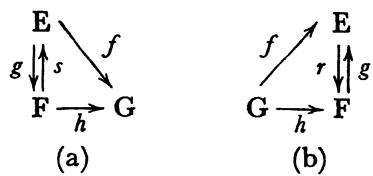
\includegraphics[keepaspectratio]{images/part001_ef8e01c05a3dcb28772fb1963be4c012627d42ff76089463ce60c193ac31650a.jpg}}

\begin{enumerate}
\def\labelenumi{(\alph{enumi})}
\setcounter{enumi}{1}
\item
  设E、F、G为集合，设g为F到E的一个单射，并设f为G到E的一个映射。则存在G到F的一个映射h，使得 \(f = g \circ h\) 当且仅当 \(f(\mathbf{G}) \subset f(\mathbf{F})\) 映射 h 由 f 唯一确定；若 r 是 g 的一个收缩，则我们有 \(h = r \circ f\) .
\item
  如果 \(f = h \circ g\) ，关系 \(g(x) = g(y)\) （其中 \(x \in \mathbf{E}\) , \(y \in \mathbf{E}\) ) 显然蕴含 \(f(x) = f(y)\) 。并且对于每个截面 \(s\) 的 \(g\) 我们拥有
\end{enumerate}

\[
h = h \circ (g \circ s) = f \circ s,
\]

，这表明 h 由 f 唯一确定。反之，假设关系 \(g(x) = g(y)\) 蕴含 \(f(x) = f(y)\) ；设 s 是 \(g\) 的一个截面，并令 \(h = f \circ s\) ；则对每个 \(x \in \mathbf{E}\) 都有 \(g(s(g(x))) = g(x)\) ，因而 \(f(s(g(x))) = f(x)\) ，即 \(h(g(x)) = f(x)\) 。因此 \(f = h \circ g\) .

\begin{enumerate}
\def\labelenumi{(\alph{enumi})}
\setcounter{enumi}{1}
\tightlist
\item
  如果 \(f = g \circ h\) ，那么显然 \(f(\mathbf{G}) \subset f(\mathbf{F})\) ，并且对于每个收缩 \(r\) 的 \(g\) 我们拥有 \(h = (r \circ g) \circ h = r \circ f\) ，这表明 \(h\) 由...唯一确定 \(f\) 相反，假设 \(f(\mathbf{G}) \subset f(\mathbf{F})\) ；令 \(r\) 为 \(g\) ，并放置 \(h = r \circ f\) ；对于每一个 \(x \in \mathbf{G}\) , 存在 \(y \in \mathbf{F}\) 使得 \(f(x) = g(y)\) ，因此
\end{enumerate}

\[
g (h (x)) = g (r (f (x))) = g (r (g (y))) = g (y) = f (x)
\]

因此 \(f = g \circ h\) .

\subsection{双自变量函数}

二元函数是指其定义域为有序对集合（或等价地，为某个乘积的子集）的函数。设 \(f\) 是这样一个函数；如果 \((x, y)\) 是定义域中的一个元素 \(f\) ，其值 \(f((x, y))\) 的 \(f\) 在元素 \((x, y)\) 通常用 \(f(x, y)\) . 设 \(f\) 是两个变量的函数， \(D\) 其定义域，以及 \(C\) 其陪域。对于每个 \(y\) 让 \(A_y\) 是所有……的集合 \(x\) 使得 \((x, y) \in D\) （即 \(\overline{D}^1\) 在 \(y\) （第1号）的截面）。映射

\[
x \rightarrow f (x, y) \quad (x \in \mathrm{A} _ {y}, f (x, y) \in \mathrm{C})
\]

称为由 \(f\) 关于第二个参数的取值 \(y\) 所定义的偏映射，并记为 \(f(\bullet, y)\) ，或 \(f(., y)\) 的复合（有时也称为 \(f_y\) ）；我们有 \(f(\bullet, y)(x) = f(x, y)\) 对于所有 \((x, y) \in D\) . 类似地，对于每一个 \(x\) 让 \(B_x\) 是所有……的集合 \(y\) 使得 \((x, y) \in D\) . 映射

\[
y \rightarrow f (x, y) \quad (y \in \mathbf {B} _ {x}, f (x, y) \in \mathbf {C})
\]

称为由 \(f\) 关于第二个参数的取值 \(x\) 关于第一个参数的取值，并记为 \(f(x, \bullet)\) ，或 \(f(x, \cdot)\) 的复合（有时也称为 \(f_x\) ）；我们有 \(f(x, \bullet)(y) = f(x, y)\) 对于所有 \((x, y) \in \mathbf{D}\) 。如果对每个 \(y\) （分别） \(x\) )，偏映射 \(f(\bullet, y)\) （分别） \(f(x, \bullet)\) )是常值映射，则称 \(f\) 不依赖于其第一个（分别地，第二个）参数；这意味着因此 \(f(x, y) = f(x', y)\) 每当 \((x, y)\) 并且 \((x', y)\) 属于 \(\mathbf{D}\) （分别） \(f(x, y) = f(x, y')\) 每当 \((x, y)\) 并且 \((x, y')\) 属于 \(\mathbf{D}\) ). 对于每一个 \(y\) 属于 \(\mathbf{D}\) 让 \(g(y)\) 表示其公共值 \(f(x, y)\) 为了 \(x \in A_y\) ；该映射 \(y \to g(y)\) 那么就是一个映射， \(\mathrm{pr}_2\mathbf{D}\) 进入。 \(\mathbf{C}\) 使得

\[
g (y) = f (x, y) \quad \text {   对   所有   } (x, y) \in D.
\]

反之，设 \(g\) 是集合 \(B\) 到集合 \(C\) 的一个映射，并设 \(A\) 为任意集合。则映射 \((x, y) \to g(y)\) （从 \(A \times B\) 到 \(C\) ）不依赖于第一个参数。

让 \(u\) 是A到C的一个映射，而 \(v\) B到D的一个映射。映射 \(z \to (u(\mathrm{pr}_1z), v(\mathrm{pr}_2z))\) 的 \(A \times B\) 进入。 \(C \times D\) 被称为 \(u\) 并且 \(v\) 到乘积集的（典范）扩张，或简称为 \(u\) 并且 \(v\) （若无混淆风险）；其值域为 \(u\langle A\rangle \times v\langle B\rangle\) 。它记作 \(u \times v\) 。如果 \(u\) 并且 \(v\) 是单射（相应地，满射），则 \(u \times v\) 是单射（相应地，满射）。如果 \(u\) 并且 \(v\) 若它们是双射的，则 \(u \times v\) 是双射的，且其逆映射为 \(\overline{u}^1 \times \overline{v}^1\) 。如果 \(u'\) 是将C映射到集合E的映射，并且如果 \(v'\) 是D到集合F的一个映射，我们有

\[
\left(u ^ {\prime} \times v ^ {\prime}\right) \circ (u \times v) = \left(u ^ {\prime} \circ u\right) \times \left(v ^ {\prime} \circ v\right).
\]

如果U、V分别是u、v的图像，那么W的图像 \(u \times v\) 是序对的集合 \(((x, y), (z, t))\) 的 \((\mathbf{A} \times \mathbf{B}) \times (\mathbf{C} \times \mathbf{D})\) 使得 \((x, z) \in \mathbf{U}\) 并且 \((y, t) \in \mathbf{V}\) ；该映射 \(((x, y), (z, t)) \to ((x, z), (y, t))\) 将W与乘积建立一一对应关系 \(U \times V\) （的一个子集 \((\mathbf{A} \times \mathbf{C}) \times (\mathbf{B} \times \mathbf{D})\) （参见§5，第5节）。

\section{一族集合的并集与交集}

\subsection{一族集合的并集与交集的定义}

设 X 是一个族（§3，第4号），I 是其指标集。为了便于对下文进行直观理解，我们将 X 称为一个集合族。若 (X, I, G) 是某个集合 E 的子集族（即其目标 G 满足关系 Y ∈ G 蕴含 Y ⊂ E），则我们将该族记为 (X\_t)\_\{t ∈ I\}(X\_t ∈ G) 或简记为 (X\_t)\_\{t ∈ I\} (§3, 第6节)；为简便起见，我们将任何以 I 为指标集的集合族记为 (X\_t)\_\{t ∈ I\}.

由于关系 \((\forall x)((\iota \in I\) 并且 \(x\in X_{\iota})\Longrightarrow (x\in X_{\iota}))\) 是真的，根据S5（第一章，§4，第2节）可知，该关系

\[
(\forall \iota) (\exists Z) (\forall x) ((\iota \in I \text { 且 } x \in X _ {\iota}) \Longrightarrow (x \in Z))
\]

是真的。根据方案S8（§1，第6节），关系 \((\exists t)(t \in I\) 并且 \(x \in X_t)\) 关于 \(x\) 是集合化的.

定义1. 设 \((\mathbf{X}_i)_{i\in I}\) 设为一个集合族（相应地，为集合E的子集族）。集合 \(\mathcal{E}_x((\exists i)(i\in I\) 并且 \(x\in \mathbf{X}_i))\) ，也就是说，所有 \(x\) 属于该族中至少一个集合的 \((\mathbf{X}_{\iota})_{\iota \in \mathbf{I}}\) ，称为该族的并集，记作 \(\bigcup \mathbf{X}_{\iota}(*)\) .

如果 \((\mathbf{X}_t)_{i\in I}\) 是集合的子集族 \(E\) ，则其并集是……的子集 \(E\) ; 注意它并不依赖于 \(E\) ，也不依赖于目标 \(\mathfrak{G}\) 该映射的 \(t\to X_t\) .

显然，如果 \(\mathbf{I} = \emptyset\) ，我们有 \(\bigcup_{i \in \mathbf{I}} \mathbf{X}_i = \emptyset\) 的集合，因为关系 \((\exists i)(i \in \mathbf{I}\) 并且 \(x \in \mathbf{X}_i)\) 此时为假。

现在假设 \(I \neq \varnothing\) 。如果 \(\alpha\) 是 I 的一个元素，关系

\[
(\forall \iota) ((\iota \in I) \Longrightarrow (x \in X _ {\iota}))
\]

蕴含 \(x \in \mathbf{X}_{\alpha}\) 。因此，根据 C52（§1，第 6 节），此关系关于 \(x\) 是集合化的。

定义 2. 设 \((\mathbf{X}_{\iota})_{\iota \in \mathbf{I}}\) 是一个集合族，其指标集 I 非空。集合 \(\mathcal{E}_x((\forall \iota)((\iota \in \mathbf{I}) \Longrightarrow (x \in \mathbf{X}_{\iota}))\) ，也就是说，所有 \(x\) 它属于该族中的每一个集合 \((\mathbf{X}_{\iota})_{\iota \in \mathbf{I}}\) ，称为该族的交集，记作 \(\bigcap_{\iota} \mathbf{X}_{\iota}\) .

如果 \(I = \varnothing\) ，关系 \((\forall t)((t \in I) \Longrightarrow (x \in X_t))\) 并未在 \(x\) ；因为这是一个真实的关系，且不存在这样的集合。 \(Y\) 使得 \(x \in Y\) 是一个真关系，因为 \(Y\) 则将是所有对象的集合（参见§1，第7号，注记）。

如果 \((\mathbf{X}_t)_{t \in \mathbf{I}}\) 是集合的子集族 \(E\) 并且如果 \(I \neq \emptyset\) ，关系“ \(x \in E\) 并且 \((\forall t)((t \in I) \Longrightarrow (x \in X_t))\) 等价于

\[
(\forall \iota) ((\iota \in I) \Longrightarrow (x \in X _ {\iota}));
\]

因此它在 \(x\) 中是集体化的，并且所有满足此关系的 \(x\) 的集合等于 \(\bigcap_{i \in I} X_i\) 。如果 \(I = \emptyset\) ，关系“ \(x \in E\) 并且 \((\forall i)((i \in I) \Longrightarrow (x \in X_i))\) ”等价于 \(x \in E\) ；因此它在 \(x\) 中是集体化的，并且所有满足此关系的 \(x\) 满足此关系的 \(E\) 因此，我们可以给出如下定义：

定义3。设 \((\mathbf{X}_{\iota})_{\iota \in \mathbf{I}}\) 设E是一个集合，E的子集族。集合

\[
\mathcal {E} _ {x} (x \in \mathrm{E} \text {   且   } (\forall \iota) ((\iota \in \mathrm{I}) \Longrightarrow (x \in \mathrm{X} _ {\iota}))),
\]

换言之，所有 \(x\) （属于 \(\mathbf{E}\) 且属于每个集合 \(\mathbf{X}_t\) ）所成的集合，称为该族的交集，记作 \(\bigcap_{i=1}^{\infty} \mathbf{X}_t\) .

因此，对于 \((\mathbf{X}_{i})_{i\in\theta}\) 的一个子集族，我们有

\[
\bigcap_ {i \in \theta} X _ {i} = E.
\]

但对于 \((\mathbf{X}_t)_{i\in I}\) 的一个子集族，若其指标集非空，则交集 \(\bigcap_{i\in I}\mathbf{X}_t\) 既不依赖于E，也不依赖于 \(\iota \to \mathbf{X}_t\) ；这证明了在定义2和定义3中使用相同记号的合理性。

命题1. 设 \((\mathbf{X}_{\mathfrak{t}})_{\mathfrak{t}\in \mathbf{I}}\) 是一族集合，并设 \(f\) 是从集合K到I的一个映射。则

\[
\bigcup_ {x \in \mathbf {K}} X _ {f (x)} = \bigcup_ {i \in I} X _ {i},
\]

并且，如果 \(\mathbf{I} \neq \emptyset\) ,

\[
\bigcap_ {x \in K} X _ {f (x)} = \bigcap_ {i \in I} X _ {i}.
\]

让 \(x\) 为 \(\bigcap_{i \in I} X_i\) . 存在一个指标 \(i \in I\) 使得 \(x \in X_i\) 。由于 \(f\langle K \rangle = I\) ，存在一个指标 \(x \in K\) 使得 \(i = f(x)\) ，由此 \(x \in X_{f(x)}\) ，从而

\[
x \in \bigcup_ {x \in \mathbf {K}} X _ {f (x)}.
\]

反之，如果 \(x \in \bigcup_{x \in \mathbb{K}} X_{f(x)}\) , 存在 \(x \in \mathbb{K}\) 使得 \(x \in X_{f(x)}\) ，因此，由于 \(f(x) \in I\) , \(x \in \bigcup_{i' \in I} X_i\) 。因此

\[
\bigcup_ {x \in \mathbb {K}} X _ {f (x)} = \bigcup_ {i \in I} X _ {i}.
\]

现在假设 \(\mathbf{I} \neq \emptyset\) ，并且让 \(x\) 为 \(\bigcap_{i \in \mathbf{I}} \mathbf{X}_i\) 。对于每个元素 \(x\) 的 \(\mathbf{K}\) 我们拥有 \(f(x) \in \mathbf{I}\) ，因此 \(x \in \mathbf{X}_{f(x)}\) ，从而

\[
x \in \bigcap_ {x \in \mathbb {K}} X _ {f (x)}.
\]

反之，设 \(x\) 为 \(\bigcap_{x \in \mathbf{K}} X_{f(x)}\) 。如果 \(\iota\) 是……的任意元素 \(I\) ，存在一个元素 \(x\) 的 \(K\) 使得 \(\iota = f(x)\) ，由此 \(x \in X_t\) 并且

因此 \(x \in \bigcap_{i \in I} X_i\) 。因此

\[
\bigcap_ {x \in \mathbf {K}} X _ {f (x)} = \bigcap_ {i \in I} X _ {i}.
\]

对于给定集合的子集族，命题1的第二部分显然在去掉限制后仍然成立。 \(I \neq \emptyset\) .

推论。设 \((\mathbf{X}_t)_{i\in \mathbf{I}}\) 设为一个集合族，使得 \(\mathbf{X}_t = \mathbf{X}_x\) 对于每一对索引 \((\mathfrak{t},\mathfrak{x})\) 然后对每一个 \(\alpha \in \mathbf{I}\) 我们拥有

\[
\bigcup_ {i \in I} X _ {i} = X _ {\alpha}, \quad \text{且} (\text{若 } I \neq \varnothing) \quad \bigcap_ {i \in I} X _ {i} = X _ {\alpha}.
\]

将命题1应用于常值映射 \(\iota\to\alpha\) 的 I 到 \(\{\alpha\}\) .

定义4. 设 \(\mathfrak{F}\) 是一组集合的集合，令 \(\Phi\) 是由恒等映射定义的集合族 \(\mathfrak{F}\) 这些集合的并集 \(\Phi\) 并且（如果 \(\mathfrak{F}\) （非空时）这些集合的交集 \(\Phi\) 分别称为集合族的并集和交集 \(\mathfrak{F}\) ，并记作 \(\bigcup_{X\sim X^{\prime}}X\) 并且 \(\bigcap_{X\sim X^{\prime}}X\) .

由命题1立即得出，如果 \((\mathbf{X}_i)_{i\in I}\) 是一个集合族，那么并集以及（若 \(I\neq \emptyset\) ) 该族的交集分别等于此族元素集合的并集与交集。

\subsection{并集与交集的性质}

如果 \((\mathbf{X}_t)_{t\in \mathbf{I}}\) 并且 \((\mathbf{Y}_t)_{t\in \mathbf{I}}\) 是具有相同指标集的集合族 \(\mathbf{I}\) ，并且如果 \(\mathbf{Y}_t\subset \mathbf{X}_t\) 对于每一个 \(t\in \mathbf{I}\) 那么显然

\[
\bigcup_ {i \in I} Y _ {i} \subset \bigcup_ {i \in I} X _ {i}, \quad \text { 且 } (\text { 若   } I \neq \emptyset) \quad \bigcap_ {i \in I} Y _ {i} \subset \bigcap_ {i \in I} X _ {i}.
\]

让 \((\mathbf{X}_t)_{t\in \mathbf{I}}\) 设为一个集合族。若 \(J\subset I\) ，我们有

\[
\bigcup_ {i \in J} X _ {i} \subset \bigcup_ {i \in I} X _ {i}, \quad \text { 且 } (\text { 若 } J \neq \emptyset) \quad \bigcap_ {i \in J} X _ {i} \supset \bigcap_ {i \in I} X _ {i}.
\]

命题2. 设 \((\mathbf{X}_{\iota})_{\iota \in \mathbf{I}}\) 为一个集合族，其指标集 I 是某个族 \((\mathrm{J}_{\lambda})_{\lambda \in \mathbf{L}}\) 的并集。则

\[
\bigcup_ {i \in I} X _ {i} = \bigcup_ {\lambda \in L} \left(\bigcup_ {i \in J _ {\lambda}} X _ {i}\right),
\]

并且（如果 \(\mathbf{L} \neq \phi\) 并且 \(J_{\lambda} \neq \phi\) 对于每一个 \(\lambda \in \mathbf{L}\) )

\[
\bigcap_ {i \in I} X _ {i} = \bigcap_ {\lambda \in L} \left(\bigcap_ {i \in J _ {\lambda}} X _ {i}\right)
\]

（并集与交集的“结合律”）。

让 \(x\) 为 \(\bigcup_{i \in I} X_i\) . 存在一个指标 \(i \in I\) 使得 \(x \in X_i\) 。由于 \(I\) 是族 \((J_\lambda)_{\lambda \in L}\) ，存在一个指标 \(\lambda \in L\) 使得 \(i \in J_\lambda\) ，由此 \(x \in \bigcup X_i\) ，并且因此

\[
x \in \bigcup_ {\lambda \in L} \left(\bigcup_ {i \in J _ {\lambda}} X _ {i}\right).
\]

反之，设 \(x\) 是此集合的一个元素。存在一个指标 \(\lambda \in L\) 使得 \(x \in \bigcup_{\iota \in J_{\lambda}} X_{\iota}\) ，因此存在一个指标 \(\iota \in J_{\lambda}\) （从而 \(\iota \in I\) ) 使得 \(x \in X_{\iota}\) ；由此得出

\[
x \in \bigcup_ {i \in I} X _ {i}.
\]

现在假设 \(L \neq \emptyset\) 并且 \(J_{\lambda} \neq \emptyset\) 对于每一个 \(\lambda \in L\) 。然后 \(I \neq \emptyset\) 。设 x 为 \(\bigcap_{i \in I} X_{i}\) 。如果 \(\lambda \in L\) ，我们有 \(x \in X_{i}\) 对于每一个 \(i \in J_{\lambda}\) （因为 \(J_{\lambda} \subset I\) ），所以 \(x \in \bigcap_{i \in J_{\lambda}} X_{i}\) 。由于最后的包含关系对所有 \(\lambda \in L\) ，x 属于 \(\bigcap_{\lambda \in L} \left( \bigcap_{i \in J_{\lambda}} X_{i} \right)\) 。反之，设 x 是后一个集合的元素，并设 i 是 I 的任意元素。存在 \(\lambda \in L\) 使得 \(i \in J_{\lambda}\) ；由于 \(x \in \bigcap_{i \in J_{\lambda}} X_{i}\) ，我们有 \(x \in X_{i}\) ，这对所有 \(i \in I\) 。因此 \(x \in \bigcap_{i \in I} X_{i}\) 都成立。这就完成了证明。

对于给定集合的子集族，命题2的第二部分在不对L作限制的情况下仍然成立，且 \(J_{\lambda}\) .

\subsection{并集与交集的像}

命题3。设 \((\mathbf{X}_t)_{t\in I}\) 是集合A的子集族，并设 \(\Gamma\) 是A与B之间的对应关系。则

\[
\Gamma \left\langle \bigcup_ {i \in I} X _ {i} \right\rangle = \bigcup_ {i \in I} \Gamma \left\langle X _ {i} \right\rangle , \quad \Gamma \left\langle \bigcap_ {i \in I} X _ {i} \right\rangle \subset \bigcap_ {i \in I} \Gamma \left\langle X _ {i} \right\rangle .
\]

关系 \((\exists x)\left(x\in \bigcup_{i\in I}X_i \text{ 且 } y\in \Gamma (x)\right)\) 等价于

\[
(\exists x) (\exists t) (t \in I \text {   且   } x \in X _ {t} \text {   且   } y \in \Gamma (x)),
\]

因此到 \((\exists \iota)(\iota \in I \text{ 且 } y \in \Gamma\langle X_{\iota}\rangle)\) ，因此等价于 \(y \in \bigcup_{\iota \in I} \Gamma\langle X_{\iota}\rangle\) ；这证明了第一个公式。至于第二个公式，我们有 \(\bigcap_{\iota \in I} X_{\iota} \subset X_{\iota}\) 对于所有 \(\iota \in I\) ，由此（§3，命题2）

\[
\Gamma \left\langle \bigcap_ {i \in I} X _ {i} \right\rangle \subset \Gamma \left\langle X _ {i} \right\rangle ,
\]

，从而

\[
\Gamma \left\langle \bigcap_ {i \in I} X _ {i} \right\rangle \subset \bigcap_ {i \in I} \Gamma \left\langle X _ {i} \right\rangle .
\]

如果 \(\Gamma\) 是任意对应关系（特别是任意函数），公式

\[
\Gamma \left\langle \bigcap_ {i \in I} X _ {i} \right\rangle = \bigcap_ {i \in I} \Gamma \left\langle X _ {i} \right\rangle
\]

通常不成立。

* 例如，在平面中 \(\mathbf{R}^2\) 这些直线的第一投影 \(y = x\) 并且 \(y = x + 1\) 等于 \(\mathbf{R}\) , 但这些直线的交集为空，因此该交集的第一投影也为空 (*)。*

然而，我们有以下重要结果：

命题4。设 \(f\) 设 为从 A 到 B 的映射，并设 \((\mathbf{Y}_t)_{t \in I}\) 为 B 的子集族。则 \(\overline{f}^1 \left\langle \bigcap_{i \in I} \mathbf{Y}_t \right\rangle = \bigcap_{i \in I} \overline{f}^1 \langle \mathbf{Y}_t \rangle\) .

为证明这一点，设 \(x\) 为 \(\bigcap_{i \in I} f^{-1} \langle Y_i \rangle\) 我们有 \(f(x) \in Y_i\) 对于所有 \(i \in I\) ，由此 \(f(x) \in \bigcap_{i \in I} Y_i\) ，并且因此

\[
x \in \overline {{f}} ^ {1} \left\langle \bigcap_ {\iota \in I} Y _ {\iota} \right\rangle .
\]

因此 \(\bigcap_{i\in I}\overline{f}^{1}(Y_{i})\subset\overline{f}^{1}\Big\langle\bigcap_{i\in I}Y_{i}\Big\rangle\) ；这一关系，连同命题3，给出了结果。

推论. 如果 \(f\) 是从 \(A\) 到 \(B\) 的单射，且 \((X_{t})_{t \in I}\) 是 \(A\) 的子集族，其指标集 \(I\) 非空，则 \(f\left\langle \bigcap_{i \in I} X_{t} \right\rangle = \bigcap_{i \in I} f\langle X_{t} \rangle\) .

因为可写成 \(f = i \circ g\) ，其中 \(i\) 是从 \(f\langle \mathbf{A} \rangle\) 到 \(\mathbf{B}\) 的典范单射，而 \(g\) 是从 \(\mathbf{A}\) 到 \(f\langle \mathbf{A} \rangle\) 的双射。如果 \(h\) 表示 \(g\) 的逆映射，则我们有 \(f\langle \mathbf{X} \rangle = \overline{h}^1\langle \mathbf{X} \rangle\) ，其中 \(\mathbf{X}\) 是 \(\mathbf{A}\) 的任意子集，因而归结为命题4。

\subsection{并集与交集的补集}

命题5。对于每一个族 \((\mathbf{X}_t)_{t\in I}\) 对于集合E的子集族，我们有

\[
\mathbb {G} _ {\mathrm{E}} \left(\bigcup_ {i \in \mathrm{I}} \mathrm{X} _ {i}\right) = \bigcap_ {i \in \mathrm{I}} \left(\mathbb {G} _ {\mathrm{E}} \mathrm{X} _ {i}\right), \quad \mathbb {G} _ {\mathrm{E}} \left(\bigcap_ {i \in \mathrm{I}} \mathrm{X} _ {i}\right) = \bigcup_ {i \in \mathrm{I}} \left(\mathbb {G} _ {\mathrm{E}} \mathrm{X} _ {i}\right).
\]

让 \(x \in \complement_{\mathbf{E}} \left( \bigcup_{i \in \mathbf{I}} \mathbf{X}_i \right)\) 。然后 \(x \in E\) 并且，对于每一个 \(i \in I\) , \(x \notin \mathbf{X}_i\) ，因此 \(x \in \complement_{\mathbf{E}} \mathbf{X}_i\) ；因此

\[
x \in \bigcap_ {i \in I} \left(\complement_ {E} X _ {i}\right).
\]

反之，设 \(x\) 为 \(\bigcap_{i \in I} (\complement_E X_i)\) ；根据交的定义，我们有 \(x \in E\) 。此外，如果我们有 \(x \in \bigcup_{i \in I} X_i\) ，那么将存在一个指标 \(x \in I\) 使得 \(x \in X_x\) ，这与假设相矛盾 \(x \in \bigcap_{i \in I} (\complement_E X_i)\) ；因此

\[
x \in \mathbb {C} _ {\mathbf {E}} \left(\bigcup_ {i \in \mathbf {I}} \mathrm{X} _ {i}\right).
\]

这证明了第一个公式；第二个公式是直接推论，鉴于关系式 \(\mathbf{G}_{\mathbf{E}}(\mathbf{G}_{\mathbf{E}}\mathbf{X})=\mathbf{X}\) 对 E 的每个子集 X 成立。

\subsection{两个集合的并集与交集}

若 A、B 是集合，我们记

\[
\mathrm{A} \cup \mathrm{B} = \bigcup_ {\mathbf {X} \in \{\mathbf {A}, \mathrm{B} \}} \mathrm{X}, \quad \mathrm{A} \cap \mathrm{B} = \bigcap_ {\mathbf {X} \in \{\mathbf {A}, \mathrm{B} \}} \mathrm{X}.
\]

显然，A ∪ B 是所有属于 A 或属于 B（或同时属于两者）的对象的集合，而 A ∩ B 是所有同时属于 A 和 B 的对象的集合。特别地， \{x, y\} = \{x\} ∪ \{y\}. 设 \{x, y, z\} = \{x, y\} ∪ \{z\}。集合 \{x, y, z\} 是仅以 x、y 和 z 为元素的集合。类似地，我们写

\[
\{x, y, z, t \} = \{x, y, z \} \cup \{t \},
\]

等等。

如果 A、B、C、D 是集合，我们写

\[
\begin{array}{c} \mathrm {A \cup B \cup C = \bigcup_ {\mathbf {X} \in \{\mathrm{A,B,C} \}} X, \quad A \cap B \cap C = \bigcap_ {\mathbf {X} \in \{\mathrm{A,B,C} \}} X;} \\ \mathrm {A \cup B \cup C \cup D = \bigcup_ {\mathbf {X} \in \{\mathrm{A,B,C,D} \}} X, \quad A \cap B \cap C \cap D = \bigcap_ {\mathbf {X} \in \{\mathrm{A,B,C,D} \}} X;} \end{array}
\]

等等。

设 A、B、C 是集合。由命题 1 和命题 2 我们推出公式

\[
\begin{array}{c} \mathbf {A} \cup \mathbf {B} = \mathbf {B} \cup \mathbf {A}, \qquad \mathbf {A} \cap \mathbf {B} = \mathbf {B} \cap \mathbf {A}, \\ \mathbf {A} \cup (\mathbf {B} \cup \mathbf {C}) = (\mathbf {A} \cup \mathbf {B}) \cup \mathbf {C} = \mathbf {A} \cup \mathbf {B} \cup \mathbf {C}, \\ \mathbf {A} \cap (\mathbf {B} \cap \mathbf {C}) = (\mathbf {A} \cap \mathbf {B}) \cap \mathbf {C} = \mathbf {A} \cap \mathbf {B} \cap \mathbf {C}. \end{array}
\]

这些公式也是准则 C24（第一章，§3，第 5 号）中所陈述定理的直接推论。类似地，可以证明公式

\[
\mathbf {A} \cup (\mathbf {B} \cap \mathbf {C}) = (\mathbf {A} \cup \mathbf {B}) \cap (\mathbf {A} \cup \mathbf {C}), \quad \mathbf {A} \cap (\mathbf {B} \cup \mathbf {C}) = (\mathbf {A} \cap \mathbf {B}) \cup (\mathbf {A} \cap \mathbf {C})
\]

（并关于交的“分配律”以及交关于并的分配律；参见 §5，第 6 号）。

关系 \(\mathbf{A} \subset \mathbf{B}\) 等价于 \(\mathbf{A} \cup \mathbf{B} = \mathbf{B}\) 以及 \(\mathbf{A} \cap \mathbf{B} = \mathbf{A}\) 。如果 \(\mathbf{A}\) 和 \(\mathbf{B}\) 是集合 \(\mathbf{E}\) 的子集，我们从命题5（或从准则C24）推导出公式

\[
\mathbb {G} _ {\mathbf {E}} (\mathbf {A} \cup \mathbf {B}) = \left(\mathbb {G} _ {\mathbf {E}} \mathbf {A}\right) \cap \left(\mathbb {G} _ {\mathbf {E}} \mathbf {B}\right), \quad \mathbb {G} _ {\mathbf {E}} (\mathbf {A} \cap \mathbf {B}) = \left(\mathbb {G} _ {\mathbf {E}} \mathbf {A}\right) \cup \left(\mathbb {G} _ {\mathbf {E}} \mathbf {B}\right);
\]

此外，我们有

\[
\mathrm{A} \cup (\mathbb {C} _ {\mathrm{E}} \mathrm{A}) = \mathrm{E}, \quad \mathrm{A} \cap (\mathbb {C} _ {\mathrm{E}} \mathrm{A}) = \varnothing .
\]

如果 \(\Gamma\) 是...之间的对应关系 \(E\) 并且 \(F\) ，并且如果 \(A, B\) 是……的子集 \(E\) ，由命题3可知

\[
\Gamma \langle \mathrm{A} \cup \mathrm{B} \rangle = \Gamma \langle \mathrm{A} \rangle \cup \Gamma \langle \mathrm{B} \rangle , \quad \Gamma \langle \mathrm{A} \cap \mathrm{B} \rangle \subset \Gamma \langle \mathrm{A} \rangle \cap \Gamma \langle \mathrm{B} \rangle ,
\]

并且，如果 \(f\) 是从 \(F\) 到 \(E\) 的映射，

\[
\overline {{{f}}} ^ {1} \langle \mathrm{A} \cap \mathrm{B} \rangle = \overline {{{f}}} ^ {1} \langle \mathrm{A} \rangle \cap \overline {{{f}}} ^ {1} \langle \mathrm{B} \rangle
\]

由命题4得出。

我们还记录以下关于补集的命题：

命题6. 设 \(f\) 是从 \(A\) 到 \(B\) 的映射。对于 \(B\) 的每一个子集 \(Y\) ，都有

\[
\overline {{{f}}} ^ {1} \langle \mathrm{B} - \mathrm{Y} \rangle = \overline {{{f}}} ^ {1} \langle \mathrm{B} \rangle - \overline {{{f}}} ^ {1} \langle \mathrm{Y} \rangle .
\]

因为 \(x\) 属于 \(\overline{f}^1\langle \mathbf{B} - \mathbf{Y}\rangle\) 当且仅当 \(f(x)\) 属于 \(\mathbf{B}\) 而不属于 \(\mathbf{Y}\) ，也就是当且仅当 \(x\) 属于 \(\overline{f}^1\langle \mathbf{B}\rangle\) 而不属于 \(\overline{f}^1\langle \mathbf{Y}\rangle\) .

推论。设 \(f\) 是从 \(\mathbf{A}\) 到 \(\mathbf{B}\) 的单射。对于 \(\mathbf{A}\) 的每一个子集 \(\mathbf{X}\) ，都有 \(f\langle \mathbf{A} - \mathbf{X}\rangle = f\langle \mathbf{A}\rangle - f\langle \mathbf{X}\rangle\) .

写成 \(f = i \circ g\) ，其中 \(i\) 是从 \(f\langle A\rangle\) 到 B 的典范单射，就把该推论化归为对 \(\overline{g}^1\) 应用命题6。

¶ 交集 X ∩ A 有时称为 X 在 A 上的迹。若 F 是一个集合族，则 F 中集合在 A 上的迹所组成的集合称为 F 在 A 上的迹。

\subsection{覆盖}

定义5. 一个集合族 \((\mathbf{X}_t)_{t \in I}\) 称为集合 E 的一个覆盖（或覆盖 E），如果 \(\mathbf{E} \subset \bigcup_{i \in I} \mathbf{X}_t\) 。如果 \((\mathbf{X}_t)_{t \in I}\) 并且 \((\mathbf{Y}_x)_{x \in K}\) 是 E 的覆盖，则这些覆盖中的第二个被称为比第一个更细（或称为第一个的加细，或加细第一个），如果对每个 \(x \in K\) , 存在 \(t \in I\) 使得

\[
\mathrm{Y} _ {x} \subset \mathrm{X} _ {i}.
\]

一个集合族 \(\Re\) 是 \(E\) 如果由恒等映射定义的集合族 \(\Re\) 是 \(E\) ，换言之，如果 \(E \subset \bigcup_{X \in \mathbb{R}} X\) .

如果 \(\Re\) , \(\Re'\) , \(\Re''\) 是E的三个覆盖，使得 \(\Re'\) 加细 \(\Re\) 并且 \(\Re''\) 加细 \(\Re'\) ，显然 \(\Re''\) 加细 \(\Re\) .

让 \((\mathbf{X}_t)_{i\in I}\) 是 E 的一个覆盖。若 J 是 I 的子集使得 \((\mathbf{X}_t)_{i\in J}\) 仍是 E 的一个覆盖，则此覆盖显然加细 \((\mathbf{X}_t)_{i\in I}\) .

让 \((\mathbf{X}_t)_{t \in I}\) 并且 \((\mathbf{Y}_x)_{x \in K}\) 是集合 \(E\) 的覆盖。则集合族 \((\mathbf{X}_t \cap \mathbf{Y}_x)_{(t,x) \in I \times K}\) 是 \(E\) 。因为如果 \(x \in E\) ，存在指标 \(t \in I\) 并且 \(x \in K\) 使得 \(x \in X_t\) 并且 \(x \in Y_x\) ，因此 \(x \in X_t \cap Y_x\) 。此外，显然覆盖 \((\mathbf{X}_t \cap Y_x)_{(t,x) \in I \times K}\) 加细每一个 \(o\) 覆盖 \((\mathbf{X}_t)_{i\in \mathbf{I}}, (\mathbf{Y}_x)_{x\in \mathbf{K}}\) 。反过来，设 \((\mathbf{Z}_{\lambda})_{\lambda \in \mathbf{L}}\) 是……的一个覆盖， \(\mathbf{E}\) 它细化每一个覆盖 \((\mathbf{X}_t)_{i\in \mathbf{I}}, (\mathbf{Y}_x)_{x\in \mathbf{K}}\) ；若 \(\lambda \in \mathbf{L}\) ，则存在指标 \(i\in \mathbf{I}\) 并且 \(x\in \mathbf{K}\) 使得 \(Z_{\lambda}\subset X_{i}\) 并且 \(Z_{\lambda}\subset Y_{x}\) ，因此 \(Z_{\lambda}\subset X_{i}\cap Y_{x}\) ；因此该覆盖 \((Z_{\lambda})_{\lambda \in \mathbf{L}}\) 是……的一个加细

\[
\left(\mathrm{X} _ {i} \cap \mathrm{Y} _ {x}\right) _ {(i, x) \in \mathrm{I} \times \mathrm{K}}.
\]

让 \((\mathbf{X}_t)_{t\in I}\) 是集合 A 的一个覆盖，并令 \(f\) 是A到集合B上的一个映射。族 \((f\langle \mathbf{X}_t\rangle)_{t\in I}\) 于是构成B的一个覆盖（命题3），称为在 \(f\) 覆盖的 \((\mathbf{X}_t)_{t\in I}\) 。如果 \(g\) 是将集合 C 映射到集合 A 的映射，该族 \((\overline{g}\langle \mathbf{X}_t\rangle)_{t\in I}\) 是C的一个覆盖，称为在 \(g\) 覆盖的 \((\mathbf{X}_t)_{t\in I}\) .

设E和F为集合，令 \((\mathbf{X}_t)_{i \in I}\) 是 E 的一个覆盖，并令 \((\mathbf{Y}_x)_{x \in K}\) 是F的一个覆盖。该族 \((\mathbf{X}_t \times \mathbf{Y}_x)_{(i,x) \in I \times K}\) 于是便是E × F的一个覆盖，称为覆盖 \((\mathbf{X}_t)_{i \in I}\) E与 \((\mathbf{Y}_x)_{x \in K}\) F的乘积。

命题7. (1) 设E是一个集合，且 \((\mathbf{X}_{\iota})_{\iota \in \mathbf{I}}\) 是E的一个覆盖。若 \(f\) 并且 \(g\) 是两个定义域为 E 的函数，使得 \(f\) 并且 \(g\) 在 \(\mathbf{E} \cap \mathbf{X}_{\iota}\) 对于每一个 \(\iota \in \mathbf{I}\) ，那么 \(f\) 并且 \(g\) 在 E 上一致。

\begin{enumerate}
\def\labelenumi{(\arabic{enumi})}
\setcounter{enumi}{1}
\item
  设 \((\mathbf{X}_i)_{i \in I}\) 是一族集合，且设 \((f_i)_{i \in I}\) 是同一目标 F 的一族映射，使得对每个 \(i \in I\) ， \(f_i\) 的定义域是 \(\mathbf{X}_i\) ，并且对于每一对 \((i, x) \in I \times I\) , \(f_i\) 和 \(f_x\) 在 \(\mathbf{X}_i \cap \mathbf{X}_x\) 上一致。那么恰好存在一个函数 \(f\) ，其定义域为 \(A = \bigcup_{i \in I} X_i\) ，目标为 F，并且它扩展了每一个函数 \(f_i (i \in I)\) .
\item
  设 \(x\) 为 \(\mathbf{E}\) 的任意元素。那么存在 \(t \in I\) 使得 \(x \in X_t\) ，由此 \(f(x) = g(x)\) 根据假设成立。
\item
  让 \(G_{i}\) 是 \(f_{i}\) 并令 \(G = \bigcup_{i \in I} G_{i}\) 的图；让我们证明 \(G\) 是一个函数图。如果 \((x, y) \in G\) 并且 \((x, y') \in G\) , 存在两个指标 \(i, x\) 在 \(I\) 使得 \((x, y) \in G_{i}\) 并且 \((x, y') \in G_{x}\) 。这意味着 \(x \in X_{i}, x \in X_{x}, y = f_{i}(x), y' = f_{x}(x)\) ；但由于 \(x \in X_{i} \cap X_{x}\) ，我们有
\end{enumerate}

\[
f _ {i} (x) = f _ {x} (x),
\]

也就是说， \(y = y'\) 。图 \(G\) 的定义域为 \(\mathrm{pr}_1 G = \bigcup_{i \in I} \mathrm{pr}_1 G_i = A\) ；因此函数 \(f = (G, A, F)\) 满足所需条件。其唯一性由命题的第一部分得出。

\subsection{划分}

定义6. 若集合A与B不相交（或不交），则称它们为不相交的（或不相交的）；若 \(\mathbf{A} \cap \mathbf{B} = \phi\) 。如果 \(\mathbf{A} \cap \mathbf{B} \neq \phi\) ，则称A与B相遇（或相交）。设 \((\mathbf{X}_{t})_{i \in I}\) 设为一个集合族。该族中的集合被称为互不相交的，如果满足条件 \(i \in I\) , \(x \in I\) , \(i \neq x\) 蕴含 \(\mathbf{X}_{t} \cap \mathbf{X}_{x} = \phi\) .

设 \(f\) 是从 \(\mathbf{A}\) 到 \(\mathbf{B}\) 的映射，并设 \((\mathbf{Y}_i)_{i\in \mathbf{I}}\) 是 \(\mathbf{B}\) 的一族两两不相交的子集。命题4表明， \((\overline{f}^1\langle \mathbf{Y}_i\rangle)_{i\in \mathbf{I}}\) （ \(\mathbf{A}\) 的子集族）中的各集合两两不相交。另一方面，如果 \((\mathbf{X}_i)_{i\in \mathbf{I}}\) 是 \(\mathbf{A}\) 的一族两两不相交的子集，则族 \((f\langle \mathbf{X}_i\rangle)_{i\in \mathbf{I}}\) 中的各集合一般并不两两不相交。

命题8. 设 \((\mathbf{X}_t)_{t \in I}\) 是一族互不相交的集合，且设 \((f_t)_{t \in I}\) 是定义域为 \(f_t\) 是 \(\mathbf{X}_t\) 对于每一个 \(t \in I\) 那么存在恰好一个函数 \(f\) ，其定义域为 \(\bigcup_{i \in I} \mathbf{X}_t\) ，目标为 F，并且它扩展了每一个函数 \(f_t\) ( \(t \in I\) ).

这是命题7的一个推论，因为 \(f_{\iota}\) 并且 \(f_{x}\) 显然在 \(\mathbf{X}_{\iota} \cap \mathbf{X}_{x} = \emptyset\) 每当 \(\iota \neq x\) .

定义7. 集合E的一个划分是E的非空互不相交子集的一个族，它们覆盖E。

例. 对于每个非空集合A，族 \((\{x\})_{x\in\mathbf{A}}\) 是A的一个划分。

如果 \((\mathbf{X}_i)_{i\in I}\) 是集合的一个划分 \(E\) ，映射 \(\iota \to X_i\) 的 \(I\) 到集合 \(\mathfrak{F}\) 的元素 \(X_i\) 的划分是双射的。因此，若 \(\mathfrak{F}\) 给定，则该划分在指标集之间的一一对应意义下是确定的。通常当我们谈到一个划分时，我们所关心的是划分中元素所构成的集合。

\subsection{集合族的并}

命题9. 设 \((\mathbf{X}_t)_{t \in I}\) 是一个集合族。则存在一个集合 \(\mathbf{X}\) ，具有如下性质： \(\mathbf{X}\) 是两两不相交集合族 \((\mathbf{X}_t')_{t \in I}\) 的并，并且对每个 \(t \in I\) 都存在一个从 \(\mathbf{X}_t\) 到 \(\mathbf{X}_t'\) 的单射。

让 \(A = \bigcup_{i \in I} X_i\) 。如果 \(i \in I\) ，映射 \(x \to (x, i)\) ( \(x \in X_i\) 是 \(X_i\) 到子集 \(X_i'\) 的 \(A \times I\) 。此外， \(X_i'\) 在第二个坐标函数下的像 \(A \times I\) 包含于集合 \(\{i\}\) ；由此得出 \(X_i' \cap X_x' = \emptyset\) 每当 \(i \neq x\) 。于是我们可以取 \(X = \bigcup_{i \in I} X_i'\) .

定义8. 设 \((\mathbf{X}_{\iota})_{\iota \in \mathbf{I}}\) 为一族集合。该族的和是这族集合的并集 \((\mathbf{X}_{\iota} \times \{\iota\})_{\iota \in \mathbf{I}}\) .

命题10。设 \((\mathbf{X}_t)_{t\in I}\) 设为一族互不相交的集合。设A为其并集，S为其和。则存在一个从A到S的双射映射。

对于每一个 \(t \in I\) ，令 \(f_{t}\) 为从 \(X_{t}\) 到 \(X_{t} \times \{t\}\) 的双射。根据命题8，存在一个从 A 到 S 的映射 f，它扩张所有映射 \(f_{t}\) 。立即可验证，f 是从 A 到 S 的双射。

滥用语言来说，集合 E 被称为一族集合的和 \((\mathbf{X}_{t})_{t\in\mathbf{I}}\) 若存在从E到该族之和的双射，如定义8中所定义的那样。

注意，如果 \((\mathbf{X}_{t})_{i\in\mathbf{I}}\) 若一族集合是任意的，命题10的论证表明存在一个从和S到并集A的映射。

\section{集合族的乘积}

\subsection{子集集合公理}

\[
(\forall \mathbf {X}) \operatorname{Coll} _ {\mathbf {Y}} (\mathbf {Y} \subset \mathbf {X}).
\]

该公理意味着，对于每个集合 X，存在一个集合，其元素是 X 的所有子集，即集合 \(\mathcal{E}_{\mathbf{Y}}(\mathbf{Y}\subset\mathbf{X})\) （§1，第4节）；该集合记为 \(\mathfrak{P}(\mathbf{X})\) 并被称为X的子集集合。显然，如果 \(X\subset X'\) ，我们有 \(\mathfrak{P}(\mathbf{X})\subset\mathfrak{P}(\mathbf{X}')\) .

设 A、B 为两个集合， \(\Gamma\) 为 A 与 B 之间的对应。函数 \(X \to \Gamma\langle X\rangle\) ( \(X \subset \mathfrak{P}(A)\) , \(\Gamma\langle X\rangle \in \mathfrak{P}(B)\) ) 称为 \(\Gamma\) 到子集集合上的典范扩张（或简称扩张），记作 \(\hat{\Gamma}\) ；它是从 \(\mathfrak{P}(A)\) 到 \(\mathfrak{P}(B)\) 的映射。如果 \(\Gamma'\) 是 B 与集合 C 之间的一个对应，则公式 \((\Gamma' \circ \Gamma)\langle X\rangle = \Gamma'\langle\Gamma\langle X\rangle\rangle\) 表明， \(\Gamma' \circ \Gamma\) 到子集集合上的扩张就是映射 \(\hat{\Gamma}' \circ \hat{\Gamma}\) .

命题1. (1) 若 \(f\) 是集合 \(\mathbf{E}\) 到集合 \(\mathbf{F}\) 的满射，则典范扩张 \(\hat{f}\) （ \(f\) 的）是从 \(\mathfrak{P}(\mathbf{E})\) 到 \(\mathfrak{P}(\mathbf{F})\) 的满射。

\begin{enumerate}
\def\labelenumi{(\arabic{enumi})}
\setcounter{enumi}{1}
\item
  如果 \(f\) 是从 \(\mathbf{E}\) 到 \(\mathbf{F}\) 的单射，则典范扩张 \(\hat{f}\) （ \(f\) 的）是从 \(\mathfrak{P}(\mathbf{E})\) 到 \(\mathfrak{P}(\mathbf{F})\) 的单射。
\item
  如果 \(s\) 是 \(f\) ，那么 \(f \circ s\) 是 \(\mathbf{F}\) ，因此 \(\hat{f} \circ \hat{s}\) 是 \(\mathfrak{P}(\mathbf{F})\) 中；因此 \(\hat{f}\) 是满射，且 \(\hat{s}\) 是 \(\hat{f}\) （§3，第8节）。
\item
  该命题在以下情形下是显然的： \(\mathbf{E} = \varnothing\) ，因为那样 \(\mathfrak{P}(\mathbf{E}) = \{\varnothing\}\) 。如果 \(\mathbf{E} \neq \varnothing\) 并且如果 \(r\) 是 \(f\) ，那么 \(r \circ f\) 是 \(\mathbf{E}\) ，因此 \(\hat{r} \circ \hat{f}\) 是 \(\mathfrak{P}(\mathbf{E})\) 中；因此 \(\hat{f}\) 是单射，并且 \(\hat{r}\) 是 \(\hat{f}\) （§3，第8节）。
\end{enumerate}

\subsection{一个集合到另一个集合的映射集}

设 E, F 为集合。从 E 到 F 的映射的图是 \(E \times F\) 的子集。因此， \(\mathfrak{P}(E \times F)\) 中由从 E 到 F 的映射的图所构成的元素集合，是 \(\mathfrak{P}(E \times F)\) 的一个子集，记为 \(F^{E}\) 。所有三元组 \(f = (G, E, F)\) （其中 \(G \in F^{E}\) ）所成的集合，就是从 E 到 F 的映射全体；它记为 \(\mathcal{F}(E, F)\) 。显然， \(G \to (G, E, F)\) 是从 \(F^{E}\) 到 \(\mathcal{F}(E, F)\) 的一个双射（称为典范双射）。这个双射使我们能够立即把关于集合 \(F^{E}\) 的每个命题转化为关于 \(\mathcal{F}(E, F)\) 的命题，反之亦然。

设 E、E'、F、F' 为集合。设 u 为从 E' 到 E 的映射，v 为从 F 到 F' 的映射。则函数 \(f \rightarrow v \circ f \circ u\) 是从 \(\mathcal{F}(\mathrm{E}, \mathrm{F})\) 到 \(\mathcal{F}(\mathrm{E}', \mathrm{F}')\) 的映射。

命题 2. (1) 若 \(u\) 是从 \(\mathbf{E}'\) 到 \(\mathbf{E}\) 的满射，而 \(v\) 是从 \(\mathbf{F}\) 到 \(\mathbf{F}'\) 的单射，则映射 \(f \to v \circ f \circ u\) 是单射。

\begin{enumerate}
\def\labelenumi{(\arabic{enumi})}
\setcounter{enumi}{1}
\tightlist
\item
  如果 \(u\) 是从 \(\mathbf{E}'\) 到 \(\mathbf{E}\) 的单射，而 \(v\) 是从 \(\mathbf{F}\) 到 \(\mathbf{F}'\) 的满射，则映射 \(f \to v \circ f \circ u\) 是满射。
\end{enumerate}

我们将假设集合 E、E'、F、F' 均为非空，否则命题显然成立。

\begin{enumerate}
\def\labelenumi{(\arabic{enumi})}
\tightlist
\item
  让 \(s\) 是……的一个截面 \(u\) 并令 \(r\) 为 \(v\) （§3，定义 11）。则 \(r \circ (v \circ f \circ u) \circ s = I_F \circ f \circ I_E = f\) ，因此
\end{enumerate}

\[
f \rightarrow v \circ f \circ u
\]

是单射的。

\begin{enumerate}
\def\labelenumi{(\arabic{enumi})}
\setcounter{enumi}{1}
\tightlist
\item
  让 \(r'\) 为 \(u\) 并令 \(s'\) 是……的一个截面 \(v\) 。对于每个映射 \(f': E' \to F'\) 我们拥有 \(v \circ (s' \circ f' \circ r') \circ u = f'\) ，这表明映射 \(f \to v \circ f \circ u\) 的满射。
\end{enumerate}

推论. 如果 \(u\) 是从 \(\mathbf{E}'\) 到 \(\mathbf{E}\) 的双射，且 \(v\) 是从 \(\mathbf{F}\) 到 \(\mathbf{F}'\) 的双射，那么 \(f \to v \circ f \circ u\) 是双射。

设 A、B、C 为三个集合，并设 f 为从 \(B \times C\) 到 A 的一个映射。对每一个 \(y \in C\) ，令 \(f(\bullet, y)\) 为从 B 到 A 的偏映射 \(x \to f(x, y)\) （§ 3，第 9 段）；函数 \(y \to f(\bullet, y)\) 是从 C 到 \(\mathcal{F}(B, A)\) 的映射。反之，对每个从 C 到 \(\mathcal{F}(B, A)\) 的映射 g，都存在唯一一个映射 \(f\) （从 \(\mathbf{B} \times \mathbf{C}\) 到 \(\mathbf{A}\) ），使得 \(g(y) = f(\bullet, y)\) （对每个 \(y \in \mathbf{C}\) ），它就是映射 \((x, y) \to (g(y))(x)\) 。因此：

命题3. 对每个映射 \(f\) （从 \(\mathbf{B} \times \mathbf{C}\) 到 \(\mathbf{A}\) ），以 \(\tilde{f}\) 表示映射 \(y \to f(\bullet, y)\) （从 \(\mathbf{C}\) 到 \(\mathcal{F}(\mathbf{B}, \mathbf{A})\) ），则函数 \(f \to \tilde{f}\) 是从 \(\mathcal{F}(\mathbf{B} \times \mathbf{C}, \mathbf{A})\) 到 \(\mathcal{F}(\mathbf{C}, \mathcal{F}(\mathbf{B}, \mathbf{A}))\) 的双射（称为典范双射）。

同样地，可定义从 \(\mathcal{F}(\mathbf{B}\times\mathbf{C},\mathbf{A})\) 到 \(\mathcal{F}(\mathbf{B},\mathcal{F}(\mathbf{C},\mathbf{A}))\) 的一个典范双射。由映射与函数图之间的一一对应，这些双射又给出从 \(\mathbf{A}^{\mathbf{B}\times\mathbf{C}}\) 到 \((\mathbf{A}^{\mathbf{B}})^{\mathbf{C}}\) （相应地， \((\mathbf{A}^{\mathbf{C}})^{\mathbf{B}})\) ）的典范双射。

\subsection{集合族乘积的定义}

让 \((\mathbf{X}_{\iota})_{\iota \in \mathbf{I}}\) 是一族集合，且设 \(\mathbf{F}\) 是一个定义域为 \(\mathbf{I}\) 使得 \(\mathbf{F}(\iota) \in \mathbf{X}_{\iota}\) 对于每一个 \(\iota \in \mathbf{I}\) 然后对每一个 \(\iota \in \mathbf{I}\) 我们拥有 \(\mathbf{F}(\iota) \in \mathbf{A} = \bigcup_{\iota \in \mathbf{I}} \mathbf{X}_{\iota}\) ，从而 \(\mathbf{F}\) 是 \(\mathfrak{P}(\mathbf{I} \times \mathbf{A})\) 因此，具有上述性质的函数图构成以下集合的一个子集 \(\mathfrak{P}(\mathbf{I} \times \mathbf{A})\) .

定义1. 设 \((\mathbf{X}_{\iota})_{\iota \in \mathbf{I}}\) 是一个集合族。函数图 \(\mathbf{F}\) （以 I 为定义域，使得 \(\mathrm{F}(\iota) \in \mathbf{X}_{\iota}\) 对于每一个 \(\iota \in \mathbf{I}\) ）组成的集合，称为该集合族 \((\mathbf{X}_{\iota})_{\iota \in \mathbf{I}}\) 的乘积，并且记作 \(\prod_{\iota \in \mathbf{I}} \mathbf{X}_{\iota}\) 。对于每一个 \(\iota \in \mathbf{I}\) , \(\mathbf{X}_{\iota}\) 称为指标为 \(\iota\) 的因子（在乘积 \(\prod_{\iota \in \mathbf{I}} \mathbf{X}_{\iota}\) 中）。映射 \(\mathrm{F} \to \mathrm{F}(\iota)\) ( \(\mathrm{F} \in \prod_{\iota \in \mathbf{I}} \mathbf{X}_{\iota}\) , \(\mathrm{F}(\iota) \in \mathbf{X}_{\iota}\) ）被称为指标为 \(\iota\) 的坐标函数（或投影），并记作 \(\operatorname{pr}_{\iota}\) .

\(F(t)\) 被称为 F 的指标为 \(t\) 的坐标（或指标为 \(t\) 的投影）；像 \(pr_{t}\langle A\rangle\) （ \(\prod_{i\in I}X_{i}\) 的子集 A 在指标为 \(t\) 的坐标函数下的像）称为 A 的指标为 \(t\) 的投影。容易验证 \(A\subset\prod_{i\in I}pr_{t}\langle A\rangle\) .

我们常使用记号 \((x_{i})_{i\in I}\) 来表示一个元素 \(\prod_{i\in I}X_{i}\) （§3，第6号）。

如果 \(\mathbf{I} = \varnothing\) ，集合 \(\prod_{i\in \mathbf{I}}\mathbf{X}_i\) 只有一个元素，即空集（§3，第4节，例1）。

如果所有因子 \(X_{t}\) 的乘积 \(\prod_{i\in I}X_{t}\) 都等于同一个集合 E，我们有 \(\prod_{i\in I}X_{t}=E^{I}\) ；这直接从定义得出。

如果 \((\mathbf{X}_t)_{t\in I}\) 是任意一族集合，并且如果 \(\mathbf{E}\) 是这样的一个集合，使得

\[
\bigcup_ {i \in I} X _ {i} \subset E,
\]

那么定义1表明 \(\prod_{i\in I}X_i\subset E^I\) ；因此，在 \(\prod_{i\in I}X_i\) 与从 \(I\) 到 \(E\) 的映射组成的一组集合（即 \(\mathcal{F}(I,E)\) 的一个子集）之间存在一个一一对应关系.

如果 \(\mathbf{I} = \{\alpha\}\) 是由单个元素组成的集合，我们有

\[
\prod_ {i \in I} X _ {i} = X _ {\alpha} ^ {\{\alpha \}};
\]

映射 \(\mathbf{F} \to \mathbf{F}(\alpha)\) 则是一个双射（称为典范双射） \(\prod_{i \in \{x\}} \mathbf{X}_i\) 到上 \(\mathbf{X}_\alpha\) .

设 A、B 为集合，且设 \(\alpha, \beta\) 为不同的对象（存在两个不同的对象，例如 \(\phi\) 并且 \(\{\phi\}\) ）。考虑图 \(\{(\alpha, A), (\beta, B)\}\) ，这显然是泛函的，并且正是该族。 \((X_{t})_{t \in [\alpha, \beta]}\) 使得 \(X_{\alpha} = A\) 并且 \(X_{\beta} = B\) 对于每一对 \((x, y) \in A \times B\) ，让 \(f_{x,y}\) 是函数图 \(\{(\alpha, x), (\beta, y)\}\) 。显然，函数 \((x, y) \to f_{x,y}\) 是 \(A \times B\) 到上 \(\prod_{t \in [\alpha, \beta]} X_t\) ；这个双射的逆映射是 \(g \to (g(\alpha), g(\beta))\) 。这两个双射被称为典范的。在下文中，我们将利用这一一对应关系，从一族集合的乘积的性质推导出两个集合的乘积的性质。

让 \((\mathbf{X}_i)_{i\in I}\) 是一族集合，其中每个集合都只含有一个元素，设为 \(\mathbf{X}_i = \{a_i\}\) ；那么乘积 \(\prod_{i\in I}\mathbf{X}_i\) 是由单一元素组成的集合 \((a_i)_{i\in I}\) .

设 E 是一个集合。将 I 中元素映到 E 中的常值映射 \(\iota \to x\) 的图组成子集 \(\Delta\) （乘积 \(\mathbf{E}^{\mathrm{I}}\) 的一个子集），称为对角线。如果 \(\overline{x}\) 表示映射 \(\iota \to x\) （其中 \(x \in \mathbf{E}\) ）的图，那么映射 \(x \to \overline{x}\) 是从 E 到 \(\Delta\) 上的双射，称为对角映射。

命题4。设 \((\mathbf{X}_i)_{i\in I}\) 是一族集合，并设 \(u\) 是从一个集合 \(K\) 到索引集 \(I\) 上的双射。如果 \(U\) 是 \(u\) 的图，那么映射 \(\mathbf{F} \to \mathbf{F} \circ U\) （从 \(\prod_{i\in I} X_i\) 到 \(\prod_{x\in K} X_{u(x)}\) ）是双射的。

让

\[
\mathrm{A} = \bigcup_ {i \in \mathbf {I}} \mathrm{X} _ {i} = \bigcup_ {\boldsymbol {x} \in \mathbf {K}} \mathrm{X} _ {u (\boldsymbol {x})}
\]

的图像（§4，命题1）。映射 \(\mathbf{F} \to \mathbf{F} \circ \mathbf{U} (\mathbf{F} \in \mathbf{A}^{\mathbf{I}})\) 是 \(\mathbf{A}^{\mathbf{I}}\) 到上 \(\mathbf{A}^{\mathbf{K}}\) （命题2）。显然，“对每个 \(\iota \in \mathbf{I}, \mathbf{F}(\iota) \in \mathbf{X}_{\iota}\) ”的条件等价于“对每个 \(x \in K, (\mathbf{F} \circ \mathbf{U})(x) \in X_{u(x)}\) ”，结论随之成立。

\subsection{部分积}

设 \((\mathbf{X}_i)_{i\in I}\) 是一族集合，并设 \(J\) 为 \(I\) 的子集。积 \(\prod_{i\in J} X_i\) 称为 \(\prod_{i\in I} X_i\) 的部分积。如果 \(f\) 是一个函数，其图像 \(F\) 是 \(\prod_{i\in I} X_i\) 的成员，那么 \(F \circ \Delta_J\) （其中 \(\Delta_J\) 是 \(J \times J\) 的对角线 ) 是 \(f\) 到 \(J\) 的限制的图。显然 \(F \circ \Delta_J \in \prod_{i\in J} X_i\) ；映射 \(F \to F \circ \Delta_J\) （从 \(\prod_{i\in I} X_i\) 到 \(\prod_{i\in I} X_i\) ）称为索引为 \(J\) 的投影，并记作 \(\operatorname{pr}_J\) .

命题5. 设 \((\mathbf{X}_{\iota})_{\iota \in \mathbf{I}}\) 是一族集合，且设 \(\mathbf{J}\) 为 \(\mathbf{I}\) 。若对每个 \(\iota \in \mathbf{I}\) 我们拥有 \(\mathbf{X}_{\iota} \neq \emptyset\) ，投影 \(\operatorname{pr}_{\mathbf{J}}\) 是……的映射 \(\prod_{\iota \in \mathbf{I}} \mathbf{X}_{\iota}\) 到上 \(\prod_{\iota \in \mathbf{J}} \mathbf{X}_{\iota}\) .

鉴于上述评论，只需证明以下命题即可：

命题6. 设 \((\mathbf{X}_{\iota})_{\iota \in \mathbf{I}}\) 为一个集合族，使得 \(\mathbf{X}_{\iota} \neq \emptyset\) 对于所有 \(\iota \in \mathbf{I}\) 成立。如果 \(g\) 是从 \(\mathbf{J} \subset \mathbf{I}\) 到 \(\mathbf{A} = \bigcup_{\iota \in \mathbf{I}} \mathbf{X}_{\iota}\) 的映射，使得 \(g(\iota) \in \mathbf{X}_{\iota}\) 对于所有 \(\iota \in \mathbf{J}\) 成立，那么存在一个 \(f\) ，它是 \(g\) 到 \(\mathbf{I}\) 的扩张，使得 \(f(\iota) \in \mathbf{X}_{\iota}\) 对于所有 \(\iota \in \mathbf{I}\) 成立.

对于每一个 \(\iota\in I-J\) 让 \(T_{\iota}\) 表示项 \(\tau_{y}(y\in X_{\iota})\) 。由于 \(X_{\iota}\neq\emptyset\) 根据假设，我们有 \(T_{\iota}\in X_{\iota}\) 对于所有 \(\iota\in I-J\) （第一章，第4节，第1号）。若G是 \(g\) 的图形，则图形 \(G\cup\left(\bigcup_{\iota\in I-J}\{(\iota,T_{\iota})\}\right)\) 是一个具有所需性质的函数的图形，这一点可以立即验证。

推论1. 设 \((\mathbf{X}_{\iota})_{\iota \in \mathbf{I}}\) 设为一族集合，使得对每个 \(\iota \in \mathbf{I}\) 我们拥有 \(\mathbf{X}_{\iota} \neq \emptyset\) 然后对每一个 \(\alpha \in \mathbf{I}\) 投影 \(\operatorname{pr}_{\alpha}\) 是……的映射 \(\prod_{\iota \in \mathbf{I}} \mathbf{X}_{\iota}\) 到上 \(\mathbf{X}_{\alpha}\) .

将命题5应用于子集 \(J = \{\alpha\}\) 的 I 并注意到 \(\mathbf{pr}_{\alpha}\) 是以下映射的复合： \(X_{\alpha}^{\{\alpha\}}\) 到上 \(X_{\alpha}\) 与映射的复合 \(\mathbf{pr}_{\{\alpha\}}\) .

推论2。设 \((\mathbf{X}_t)_{i \in \mathbf{I}}\) 是一个集合族。则 \(\prod_{i \in \mathbf{I}} \mathbf{X}_t = \varnothing\) 当且仅当存在 \(i \in \mathbf{I}\) 使得 \(\mathbf{X}_t = \varnothing\) .

如果我们有 \(X_{t} \neq \varnothing\) 对于每一个 \(t \in I\) ，则由推论1可知 \(\prod_{i \in I} X_{t} \neq \varnothing\) ；反之，如果 \(\prod_{i \in I} X_{t} \neq \varnothing\) ，关系 \(\Pr_{\alpha}\left(\prod_{i \in I} X_{t}\right) \subset X_{\alpha}\) 表明 \(X_{\alpha} \neq \varnothing\) 对于每一个 \(\alpha \in I\) .

因此，如果我们有一个族 \((\mathbf{X}_{t})_{t\in\mathbf{I}}\) 对于非空集合族，我们可以引入（作为辅助常项）一个定义域为I的函数f，使得 \(f(t)\in\mathbf{X}_{t}\) 对于所有 \(t\in I\) 在实践中人们常说：“取一个元素 \(x_{t}\) 在每个 \(X_{t}\) 直观地说，我们因此“选择”了一个元素。 \(x_{t}\) 在每个集合中 \(X_{t}\) ；逻辑符号的引入 \(\tau\) 并且规范其使用的准则使我们无需制定一个“选择公理”来使这一操作合法化（参见结果概要，第4节，第10条）。

推论3。设 \((\mathbf{X}_t)_{i\in I}\) 并且 \((\mathbf{Y}_t)_{i\in I}\) 是两族具有相同指标集I的集合。如果 \(\mathbf{X}_t\subset \mathbf{Y}_t\) 对于每一个 \(i\in I\) ，那么

\[
\prod_ {i \in I} X _ {i} \subset \prod_ {i \in I} Y _ {i}.
\]

反之，如果 \(\prod_{i\in I}X_i\subset \prod_{i\in I}Y_i\) ，并且如果 \(X_{i}\neq \emptyset\) 对于每一个 \(i\in I\) ，那么 \(X_{i}\subset Y_{i}\) 对于每一个 \(i\in I\) .

第一个断言是显然的，第二个断言则来自命题1的推论5，因为此时对每个 \(\alpha \in I\) ,

\[
\mathrm{X} _ {\alpha} = \operatorname{pr} _ {\alpha} \left(\prod_ {i \in \mathrm{I}} \mathrm{X} _ {i}\right) \subset \operatorname{pr} _ {\alpha} \left(\prod_ {i \in \mathrm{I}} \mathrm{Y} _ {i}\right) = \mathrm{Y} _ {\alpha}.
\]

\subsection{集合乘积的结合性}

命题7。设 \((\mathbf{X}_t)_{t \in \mathbf{I}}\) 设为一个集合族，其指标集 I 不是空集。设 \((\mathrm{J}_{\lambda})_{\lambda \in \mathbf{L}}\) 是 I 的一个划分。则映射

\[
f \rightarrow (\mathrm{pr} _ {\mathbf {J} _ {\lambda}} f) _ {\lambda \in \mathbf {L}}
\]

的 \(\prod_{i\in I}X_i\) 到乘积集合 \(\prod_{\lambda \in L}\left(\prod_{i\in J_\lambda}X_i\right)\) 是双射（集合乘积的“结合性”）。

由 \(\mathbf{pr}_{\mathbf{J}_{\lambda}}f\) 作为图形为 \(f\) 的函数的限制的图形这一解释（第 4 节），可知映射 \(f \to (\mathbf{pr}_{\mathbf{J}_{\lambda}}f)_{\lambda \in \mathbf{L}}\) 是双射这一陈述意味着，对于每个族 \((v_{\lambda})_{\lambda \in \mathbf{L}}\) ，其中 \(v_{\lambda}\) 是从 \(\mathbf{J}_{\lambda}\) 到 \(\bigcup_{i\in I}\mathbf{X}_i\) 的映射，存在唯一的映射 \(u\)

将 I 映入 \(\bigcup_{i\in I}X_i\) ，使得 \(v_{\lambda}\) 是 \(u\) 到 \(J_{\lambda}\) 的限制，对于每一个 \(\lambda\in L\) 。但这是假设 \((J_{\lambda})_{\lambda\in L}\) 是 I 的一个划分（§4，命题 8）的推论。

命题 7 中定义的双射及其逆双射称为典范双射。

\minorheading{注记}

\begin{enumerate}
\def\labelenumi{(\arabic{enumi})}
\tightlist
\item
  让 \(\alpha, \beta\) 是两个不同的对象，令 \((J_{\lambda})_{\lambda \in \{\alpha, \beta\}}\) 是I的一个划分为两个集合 \(J_{\alpha}, J_{\beta}\) 因此我们得到一个一一映射（仍称为典范映射）的乘积 \(\prod_{i \in I} X_i\) 到上 \(\left(\prod_{i \in J_{\alpha}} X_i\right) \times \left(\prod_{i \in J_{\beta}} X_i\right)\) 通过构成典范映射的复合 \(\prod_{\lambda \in \{\alpha, \beta\}} \left(\prod_{i \in J_{\lambda}} X_i\right)\) 到上 \(\left(\prod_{i \in J_{\alpha}} X_i\right) \times \left(\prod_{i \in J_{\beta}} X_i\right)\) 以及 \(\prod_{i \in I} X_i\) 到上 \(\prod_{\lambda \in \{\alpha, \beta\}} \left(\prod_{i \in J_{\lambda}} X_i\right)\) 。如果 \(X_i\) 是一个集合，对于每个 \(i \in J_{\beta}\) ，那么 \(\operatorname{pr}_{J_{\alpha}}\) 是 \(\prod_{i \in I} X_i\) 到上 \(\prod_{i \in J_{\beta}} X_i\) .
\end{enumerate}

\[
\iota \in J _ {\alpha}
\]

\begin{enumerate}
\def\labelenumi{(\arabic{enumi})}
\setcounter{enumi}{1}
\tightlist
\item
  让 \(\alpha, \beta, \gamma\) 是三个对象，其中任意两个都不相等（存在这样的三个对象；例如， \(\phi, \{\phi\}, \{\{\phi'\}\}\) ），并设 A、B、C 为集合。考虑函数图 \(\{(\alpha, A), (\beta, B), (\gamma, C)\}\) ，即集合族 \((X_{t})_{t \in \{\alpha, \beta, \gamma\}}\) 使得 \(X_{\alpha} = A\) , \(X_{\beta} = B\) , \(X_{\gamma} = C\) 。对于由两个集合 \(\{\alpha, \beta, \gamma\}\) 构成的 \(\{\alpha, \beta\}\) 并且 \(\{\gamma\}\) 的分划，存在一个从 \(\prod X_{t}\) 到乘积的典范双射
\end{enumerate}

\(\iota \in \{\alpha, \beta, \gamma\}\)

\[
\left(\prod_ {\iota \in \{\alpha , \beta \}} \mathbf {X} _ {\iota}\right) \times \mathbf {X} _ {\gamma} ^ {\{\gamma \}},
\]

因此是一个双射（同样称为典范的） \(\prod_{\iota \in \{\alpha, \beta, \gamma\}} \mathbf{X}_{\iota}\) 到上 \(\mathbf{A} \times \mathbf{B} \times \mathbf{C}\) ( \(\S 2\) ，编号2）它将每个图 \(f \in \prod_{\iota \in \{\alpha, \beta, \gamma\}} \mathbf{X}_{\iota}\) 变换为元素 \((f(\alpha), f(\beta), f(\gamma))\) 的 \(\mathbf{A} \times \mathbf{B} \times \mathbf{C}\) 。根据命题4，因此我们可以将六个集合中的任意两个 \(\mathbf{A} \times \mathbf{B} \times \mathbf{C}\) , \(\mathbf{B} \times \mathbf{C} \times \mathbf{A}\) , \(\mathbf{C} \times \mathbf{A} \times \mathbf{B}\) , \(\mathbf{B} \times \mathbf{A} \times \mathbf{C}\) , \(\mathbf{A} \times \mathbf{C} \times \mathbf{B}\) , \(\mathbf{C} \times \mathbf{B} \times \mathbf{A}\) 建立一一对应关系。

\subsection{分配律公式}

命题8. 设 \(((\mathbf{X}_{\lambda,1})_{i\in \mathbf{J}_2})_{\lambda \in \mathbf{L}}\) 为一个（以L为指标集的）集合族的族。假设 \(\mathbf{L}\neq \emptyset\) 以及 \(J_{\lambda}\neq \emptyset\) 对于每一个 \(\lambda \in \mathbf{L}\) 成立. 设

\[
\mathrm{I} = \prod_ {\lambda \in \mathrm{L}} \mathrm{J} _ {\lambda} \neq \emptyset .
\]

于是我们有

\[
\begin{array}{l} \bigcup_ {\lambda \in \mathbf {L}} \Big (\bigcap_ {t \in \mathbf {J} _ {\lambda}} \mathbf {X} _ {\lambda , t} \Big) = \bigcap_ {f \in \mathbf {I}} \Big (\bigcup_ {\lambda \in \mathbf {L}} \mathbf {X} _ {\lambda , f (\lambda)} \Big), \\ \bigcap_ {\lambda \in \mathbf {L}} \Big (\bigcap_ {t \in \mathbf {J} _ {\lambda}} \mathbf {X} _ {\lambda , t} \Big) = \bigcup_ {f \in \mathbf {I}} \Big (\bigcap_ {\lambda \in \mathbf {L}} \mathbf {X} _ {\lambda , f (\lambda)} \Big) \end{array}
\]

（并集对交集的“分配律”，以及交集对并集的分配律）。

设 \(x\) 为 \(\bigcup_{\lambda \in L} \left( \bigcap_{i \in J_{\lambda}} X_{\lambda, i} \right)\) 的一个元素，并令 \(f\) 为 1 的任意元素。存在一个指标 \(\lambda\) 使得 \(x \in \bigcap_{i \in J_{\lambda}} X_{\lambda, i}\) ；因此 \(x \in X_{\lambda, f(\lambda)}\) ，从而

\[
x \in \bigcup_ {\lambda \in \mathbf {L}} \mathrm{X} _ {\lambda , f (\lambda)}.
\]

由于这对每个 \(f \in I\) ，我们有

\[
x \in \bigcap_ {f \in I} \left(\bigcup_ {\lambda \in L} X _ {\lambda , f (\lambda)}\right).
\]

反之，设 \(x\) 是一个不属于该集合的对象

\[
\bigcup_ {\lambda \in L} \left(\bigcap_ {i \in J _ {\lambda}} X _ {\lambda , i}\right).
\]

于是对每个 \(\lambda \in L\) 我们拥有 \(x \notin \bigcap_{\iota \in J_{\lambda}} X_{\lambda, \iota}\) ，这意味着集合 \(J_{\lambda}'\) 指标 \(\iota \in J_{\lambda}\) 使得 \(x \notin X_{\lambda, \iota}\) 对每个 \(\lambda \in L\) 都不是空的。根据命题5、推论2，存在一个函数图 \(f\) ，其定义域为 \(L\) 使得对于每一个 \(\lambda \in L\) 我们拥有 \(f(\lambda) \in J_{\lambda}'\) 因此 \(f \in I\) 并且 \(x \notin X_{\lambda, f(\lambda)}\) 对于每一个 \(\lambda \in L\) ；因此

\[
x \notin \bigcup_ {\lambda \in \mathbf {L}} \mathrm{X} _ {\lambda , f (\lambda)}
\]

并且从而

\[
x \notin \bigcap_ {f \in I} \left(\bigcup_ {\lambda \in L} X _ {\lambda , f (\lambda)}\right).
\]

这就完成了第一个公式的证明。第二个公式通过将第一个公式应用于族 \(\left((\mathbb{C}_{\Lambda}X_{\lambda,t})_{t\in J_{\lambda}}\right)_{\lambda \in L}\) 而得出，其中 A 表示并集 \(\bigcap_{\lambda \in L}\left(\bigcap_{t\in J_{\lambda}}X_{\lambda}\right)\) .

推论。设 \((\mathbf{X}_i)_{t\in \mathbf{I}}\) 并且 \((\mathbf{Y}_x)_{x\in \mathbb{K}}\) 是两族集合，其指标集 I, K 非空。则

\[
\begin{array}{l} \left(\bigcap_ {i \in I} X _ {i}\right) \cup \left(\bigcap_ {x \in K} Y _ {x}\right) = \bigcap_ {(i, x) \in I \times K} (X _ {i} \cup Y _ {x}), \\ \left(\bigcup_ {i \in I} X _ {i}\right) \cap \left(\bigcup_ {x \in K} Y _ {x}\right) = \bigcup_ {(i, x) \in I \times K} (X _ {i} \cap Y _ {x}). \end{array}
\]

让 \(\alpha, \beta\) 是两个不同的对象；将命题 8 的公式（以 \(L = \{\alpha, \beta\}\) , \(J_{\alpha} = I\) , \(J_{\beta} = K\) ) 到该族 \(((Z_{\lambda, \mu})_{\mu \in J_{\lambda}})_{\lambda \in L}\) ，其中 \(Z_{\alpha, \iota} = X_{\iota}\) 对于所有 \(\iota \in I\) 并且 \(Z_{\beta, x} = Y_{x}\) 对于每一个 \(x \in K\) . 由于典范双射的存在， \(\prod_{\lambda \in L} J_{\lambda}\) 到上 \(I \times K\) (no. 3) 且由§4的命题1，我们得到所述公式。

命题9. 设 \(((\mathbf{X}_{\lambda, t})_{t \in \mathbf{J}_{\lambda}})_{\lambda \in \mathbf{L}}\) 为一族（以指标集 L 为指标）的集合族。设 \(\mathbf{I} = \prod_{\lambda \in \mathbf{J}_{\lambda}} \mathbf{J}_{\lambda}\) 。然后

\[
\prod_ {\lambda \in L} \left(\bigcup_ {i \in J _ {\lambda}} X _ {\lambda , i}\right) = \bigcup_ {f \in I} \left(\prod_ {\lambda \in L} X _ {\lambda , f (\lambda)}\right)
\]

并且（如果 \(\mathbf{L} \neq \phi\) 并且 \(\mathbf{J}_{\lambda} \neq \phi\) 对于每一个 \(\lambda \in \mathbf{L}\) )

\[
\prod_ {\lambda \in \mathrm{L}} \left(\bigcap_ {i \in \mathrm{J} _ {\lambda}} \mathrm{X} _ {\lambda , i}\right) = \bigcap_ {f \in \mathrm{I}} \left(\prod_ {\lambda \in \mathrm{L}} \mathrm{X} _ {\lambda , f (\lambda)}\right)
\]

（乘积对并集和交集的“分配律”）。

第一个公式在以下情况下显然成立：如果 \(L = \emptyset\) 或者如果 \(J_{\lambda} = \emptyset\) 对于某个 \(\lambda \in L\) 。如果不是，设 \(g\) 为 \(\prod_{\lambda \in L} \left( \bigcap_{t \in J_{\lambda}} X_{\lambda, t} \right)\) 对于每一个 \(\lambda \in L\) 存在一个指标 \(t \in J_{\lambda}\) 使得 \(g(\lambda) \in X_{\lambda, t}\) ；换句话说，该集合 \(H_{\lambda}\) 指标 \(t \in J_{\lambda}\) 使得 \(g(\lambda) \in X_{\lambda, t}\) 非空。因此，根据命题5的推论2，存在一个函数图。 \(f\) ，其定义域为 \(L\) 使得

\[
f (\lambda) \in \mathrm{H} _ {\lambda}
\]

对于每一个 \(\lambda \in L\) ，即 \(g(\lambda) \in X_{\lambda, f(\lambda)}\) 。因此我们有 \(g \in \prod_{\lambda \in L} X_{\lambda, f(\lambda)}\) ，从而 \(g \in \bigcup_{f \in I} \left( \prod_{\lambda \in L} X_{\lambda, f(\lambda)} \right)\) 。反之，若

\[
g \in \bigcup_ {f \in \mathbf {I}} \left(\prod_ {\lambda \in \mathbf {L}} \mathrm{X} _ {\lambda , f (\lambda)}\right),
\]

存在一个函数图 \(f \in I\) 使得对于每一个 \(\lambda \in L\) 我们拥有

\[
g (\lambda) \in \mathbf {X} _ {\lambda , f (\lambda)}
\]

并且，更不用说， \(g(\lambda) \in \bigcup_{t \in J_1} X_{\lambda,t}\) 。这就完成了第一个公式的证明。第二个公式的证明类似但更简单，我们留给读者。

推论1。假设 \(\mathbf{L} \neq \emptyset\) 以及 \(J_{\lambda} \neq \emptyset\) 对于每一个 \(\lambda \in L\) . 如果对于 \(e\) achindex \(\lambda \in L\) 族 \((X_{\lambda, t})_{t \in J_{\lambda}}\) 是 \(X_{\lambda} = \bigcup_{t \in J_{\lambda}} X_{\lambda, t}\) 的一个划分，则族 \(\left( \prod_{\lambda \in L} X_{\lambda, f(\lambda)} \right)_{f \in I}\) 是 \(\prod_{\lambda \in L} X_{\lambda}\) 的一个划分.

如果我们设

\[
\mathrm{P} _ {f} = \prod_ {\lambda \in \mathbf {L}} \mathrm{X} _ {\lambda , f (\lambda)},
\]

那么，根据命题9的第一个公式，只需证明 \(\mathbf{P}_f \neq \emptyset\) 对于所有 \(f \in \mathbf{I}\) ，以及 \(\mathbf{P}_f \cap \mathbf{P}_g = \emptyset\) 每当 \(f\) 和 \(g\) 是 \(\mathbf{I}\) 的不同元素。第一点由命题5的推论2得出。至于第二点，如果 \(f \neq g\) , 存在 \(\lambda \in \mathbf{L}\) 使得

\[
f (\lambda) \neq g (\lambda)
\]

因此，根据假设， \(\mathbf{X}_{\lambda,f(\lambda)} \cap \mathbf{X}_{\lambda,g(\lambda)} = \varnothing\) 。由此可知，不存在属于 \(P_{f} \cap P_{g}\) 的图；因为如果G是这样的图，我们就会有 \(\mathbf{G}(\lambda) \in \mathbf{X}_{\lambda,f(\lambda)} \cap \mathbf{X}_{\lambda,g(\lambda)} = \varnothing\) ，这是荒谬的。

推论2。设 \((\mathbf{X}_i)_{i\in \mathbf{I}}\) 并且 \((\mathbf{Y}_x)_{x\in \mathbb{K}}\) 为两个集合族。则

\[
\left(\bigcup_ {i \in I} X _ {i}\right) \times \left(\bigcup_ {x \in K} Y _ {x}\right) = \bigcup_ {(i, x) \in I \times K} (X _ {i} \times Y _ {x})
\]

并且，如果I和K非空，

\[
\left(\bigcap_ {i \in I} X _ {i}\right) \times \left(\bigcap_ {x \in K} Y _ {x}\right) = \bigcap_ {(i, x) \in I \times K} (X _ {i} \times Y _ {x}).
\]

证明遵循命题8推论证明的模式。

命题10。设 \((\mathbf{X}_{t,x})_{(t,x)\in \mathbf{I}\times \mathbf{K}}\) 是一个集合族，其指标集是两个集合 I 和 K 的乘积。如果 \(\mathbf{K}\neq \emptyset\) ，我们有

\[
\bigcap_ {x \in \mathbf {K}} \left(\prod_ {i \in I} X _ {i, x}\right) = \prod_ {i \in I} \left(\bigcap_ {\mathbf {K} \in x} X _ {i, x}\right).
\]

待证等式两边都是函数图。一个图 \(f\) 属于左边当且仅当，对每个 \(x \in \mathbf{K}\) , \(f \in \prod_{i \in I} X_{i,x}\) ；也就是说，当且仅当 \(f(t) \in X_{t,x}\) 对于所有 \((t,x) \in I \times K\) 成立。因为 \(f\) 要属于右侧，必要且充分的条件是 \(f(t) \in \bigcap_{x \in K} X_{t,x}\) 对于每一个 \(t \in I\) ，即 \(f(t) \in X_{t,x}\) 对于每一对 \((t, x) \in I \times K\) 都成立。这就完成了证明。

推论。设 \((\mathbf{X}_t)_{t\in \mathbf{I}}\) 并且 \((\mathbf{Y}_t)_{t\in \mathbf{I}}\) 为两个具有相同指标集的集合族 \(\mathbf{I}\neq \emptyset\) 。然后

\[
\begin{array}{l} \left(\prod_ {i \in I} X _ {i}\right) \cap \left(\prod_ {i \in I} Y _ {i}\right) = \prod_ {i \in I} (X _ {i} \cap Y _ {i}), \\ \left(\bigcap_ {i \in I} X _ {i}\right) \times \left(\bigcap_ {i \in I} Y _ {i}\right) = \bigcap_ {i \in I} (X _ {i} \times Y _ {i}). \end{array}
\]

将命题10应用于K（相应地，I）是由两个不同元素构成的集合的情形。

\subsection{映射到乘积的扩展}

定义 2. 设 \((\mathbf{X}_t)_{t \in I}, (\mathbf{Y}_t)_{t \in I}\) 是两个集合族，并且设 \((g_t)_{t \in I}\) 为一个具有相同指标集I的函数族，使得 \(g_t\) 是从 \(\mathbf{X}_t\) 到 \(\mathbf{Y}_t\) 的映射，对于每一个 \(t \in I\) 。对于每一个 \(f \in \prod_{t \in I} \mathbf{X}_t\) ，令 \(u_f\) 为函数 \(t = g_t(f(t))\) ( \(t \in I\) )的图像，它是 \(\prod_{t \in I} \mathbf{Y}_t\) 的一个元素。映射 \(f \to u_f\) （从 \(\prod_{t \in I} \mathbf{X}_t\) 到 \(\prod_{t \in I} \mathbf{Y}_t\) ）被称为映射族 \((g_t)_{t \in I}\) 到乘积的典范扩张（或简称为扩张）；它有时也被称为映射族 \((g_t)_{t \in I}\) 的乘积.

当使用指标记号时，族 \((g_{i})_{i\in I}\) 的乘积是函数 \((x_{i})_{i\in I}\to (g_{i}(x_{i}))_{i\in I}\) ；它有时记作 \((g_{i})_{i\in I}\) .

如果 \(\mathbf{I} = \{\alpha, \beta\}\) ，其中 \(\alpha\) 和 \(\beta\) 是不同的，则映射族 \((g_t)_{t \in \mathbf{I}}\) 到乘积的扩张正是 \(\psi \circ (g_\alpha \times g_\beta) \circ \varphi\) ，其中 \(\varphi\) 表示从 \(\prod_{i \in \mathbf{I}} \mathbf{X}_i\) 到上 \(\mathbf{X}_\alpha \times \mathbf{X}_\beta\) （第3节）的典范映射，且 \(\psi\) 表示从 \(\mathbf{Y}_\alpha \times \mathbf{Y}_\beta\) 到上 \(\prod_{i \in \mathbf{I}} \mathbf{Y}_i\) 的典范映射.

命题11。设 \((\mathbf{X}_t)_{t \in I}, (\mathbf{Y}_t)_{t \in I}, (\mathbf{Z}_t)_{t \in I}\) 是三个集合族，并设 \((g_t)_{t \in I}, (g_t')_{t \in I}\) 是两个函数族，它们具有相同的指标集，使得 \(g_t\) 是从 \(\mathbf{X}_t\) 到 \(\mathbf{Y}_t\) 的映射并且 \(g_t'\) 是从 \(\mathbf{Y}_t\) 到 \(\mathbf{Z}_t\) 的一个映射，对每个 \(t \in I\) . 设 \(g\) 和 \(g'\) 为族 \((g_t)_{t \in I}\) 和 \((g_t')_{t \in I}\) 到乘积的扩张。然后族 \((g_t' \circ g_t)_{t \in I}\) 到乘积的扩张等于 \(g'\circ g\) .

这直接由定义2得出。

推论。设 \((\mathbf{X}_i)_{i\in I}, (\mathbf{Y}_i)_{i\in I}\) 是两个集合族，并设 \((g_i)_{i\in I}\) 是一个函数族。如果 \(g_i\) 是从 \(\mathbf{X}_i\) 到 \(\mathbf{Y}_i\) 的一个单射（相应地，满射），对于每一个 \(i\in I\) ，那么 \(g\) （族 \((g_i)_{i\in I}\) 到乘积的扩张）是从 \(\prod_{i\in I} \mathbf{X}_i\) 到 \(\prod_{i\in I} \mathbf{Y}_i\) 的一个单射（相应地，满射）.

\begin{enumerate}
\def\labelenumi{(\arabic{enumi})}
\item
  让我们假设 \(X_{i} \neq \emptyset\) 对于每一个 \(i \in I\) ；否则结果是平凡的。假设 \(g_{i}\) 对每个 \(i \in I\) ，并且让 \(r_{i}\) 为 \(g_{i}\) （§3，第8号，定义11），因此 \(r_{i} \circ g_{i}\) 是 \(X_{i}\) 。设 r 为族 \((r_{i})_{i \in I}\) ；由于 \(r \circ g\) 是恒等映射族到乘积的扩展 \(I_{X_{i}}\) , \(r \circ g\) 是 \(\prod_{i \in I} X_{i}\) ，因此 g 是单射（§3，命题8）。
\item
  假设 \(g_{i}\) 是……的满射 \(X_{i}\) 到上 \(Y_{i}\) 对于每一个 \(i \in I\) ，并且让 \(s_{i}\) 是……的一个截面 \(g_{i}\) ( \(\S 3\) ，第8号，定义11），因此 \(g_{i} \circ s_{i}\) 是 \(Y_{i}\) 。如果 \(s\) 是族到乘积的扩张 \((s_{i})_{i \in I}\) ，那么 \(g \circ s\) 是恒等映射族到乘积的扩展 \(I_{Y_{i}}\) 并且因此是 \(\prod_{i \in I} Y_{i}\) ；因此 \(g\) 是满射（ \(\S 3\) ，命题8）。
\end{enumerate}

让 \((\mathbf{X}_i)_{i\in I}\) 设为一个集合族，并令 E 为一个集合。对于每个映射 \(f\) 将E映入 \(\prod_{i\in I} \mathbf{X}_i\) , \(\operatorname{pr}_i \circ f\) 是E到 \(\mathbf{X}_i\) 。如果 \(\overline{f}\) 是该映射族到乘积的延拓，且若 \(d\) 是E到 \(\mathbf{E}^{\mathrm{I}}\) 的对角映射，则显然 \(f = \overline{f} \circ d\) 。反过来，设 \((f_{t})_{t \in \mathbf{I}}\) 是这样一个函数族，使得 \(f_{t}\) 是E到 \(\mathbf{X}_{t}\) 对于每一个 \(i \in \mathbf{I}\) ，并且让 \(\overline{f}\) 设为此族到乘积的扩张；于是我们有 \(\mathbf{pr}_{t} \circ (\overline{f} \circ d) = f_{t}\) 对于每一个 \(t \in \mathbf{I}\) . 滥用语言，该映射 \(\overline{f} \circ d\) 也写作 \((f_{t})_{t \in \mathbf{I}}\) 。这样，我们就定义了该集合的一一映射 \(\prod_{i \in \mathbf{I}} \mathbf{X}_{t}^{\mathbf{E}}\) 到集合 \(\left(\prod_{i \in \mathbf{I}} \mathbf{X}_{t}\right)^{\mathbf{E}}\) 此映射及其逆映射被称为典范的。

\section{等价关系}

原则上，从现在起我们将不再使用粗斜体字母来表示未确定的组合；读者将能轻易地从上下文中辨别出适用于未确定字母或关系的断言。

\subsection{等价关系的定义}

让 \(R\{x, y\}\) 是一个关系，其中x和y是不同的字母。关系R被称为（关于字母x和y）对称的，如果

\[
\mathrm{R} \{x, y \} \Longrightarrow \mathrm{R} \{y, x \}.
\]

如果是这样，通过将x和y替换为两个字母 \(x'\) 并且 \(y'\) ，它们彼此不同且与R中出现的所有字母都不同，然后依次将y和x替换为 \(x'\) 并且 \(y'\) ，我们可以看到

\[
\mathrm{R} \left\{y, x \right\} \Longrightarrow \mathrm{R} \left\{x, y \right\}.
\]

因此， \(\mathbb{R}\{x, y\}\) 并且 \(\mathbb{R}\{y, x\}\) 是等价的。设 \(z\) 为一个未出现在 \(\mathbb{R}\) 。关系 \(\mathbb{R}\) 被称为可传递的（关于字母） \(x, y\) ）如果我们有

\[
(\mathrm{R} \{x, y \} \text {   且   } \mathrm{R} \{y, z \}) \Longrightarrow \mathrm{R} \{x, z \}.
\]

例子。关系 x = y 是对称且传递的。关系 \(X \subset Y\) 是传递的但不对称。关系 \(X \cap Y = \varnothing\) 是对称的但不传递的。

如果 \(\mathbf{R}\{x, y\}\) 既对称又传递，就称它是（关于字母 \(x\) 和 \(y\) 的）等价关系。在这种情况下，记号 \(x \equiv y \pmod{\mathbf{R}}\) 有时用作 \(\mathbf{R}\{x, y\}\) 的同义记号；读作“ \(x\) 等价于 \(y\) （模 \(\mathbf{R}\) ）”。如果 \(\mathbf{R}\) 是等价关系，则有 \(\mathbf{R}\{x, y\} \Longrightarrow (\mathbf{R}\{x, x\} \text{ 且 } \mathbf{R}\{y, y\})\) ，因为 \(\mathbf{R}\{x, y\}\) 蕴含 \(\mathbf{R}\{y, x\}\) ，而由定义， \((\mathbf{R}\{x, y\} \text{ 且 } \mathbf{R}\{y, x\})\) 蕴含 \((\mathbf{R}\{x, x\} \text{ 且 } \mathbf{R}\{y, y\})\) 。

让 \(\mathbf{R}\{x, y\}\) 是一个关系；它被称为在 \(\mathbf{E}\) （就字母而言） \(x, y\) ) 如果该关系 \(\mathbf{R}\{x, x\}\) 等价于 \(x \in \mathbf{E}\) 。如果关于 \(\mathbf{E}\) 不存在可能的歧义，则简言之（滥用语言地）称 \(\mathbf{R}\) 是自反的。

¶ E上的等价关系被定义为在E上自反的等价关系。如果R\{x, y\} 是 E 上的一个等价关系，我们有 R\{x, y\} \(\Longrightarrow\) ((x, y) ∈ E × E)，因此 R 有一个图（关于字母 x, y）。反之，假设等价关系 R\{x, y\} 有一个图 G。注意关系 R\{x, x\} 等价于关系 (∃y)R\{x, y\}；因为前者蕴含后者（第一章，§4，第2节，方案S5），反之亦然，由于R\{x, y\} 蕴含R\{x, x\}，(∃y)R\{x, y\} 意味着存在某个y使得R成立\{x, x\} 因此也有R\{x, x\}。因此R\{x, x\} 等价于 \(x \in pr_{1}G\) ，且因此R是 \(pr_{1}G\) .

集合 E 上的一个等价关系是一个对应，其源与目标都等于 E，且其图形 F 使得关系 \((x, y) \in \mathbb{F}\) 是 E 上的一个等价关系。

\minorheading{示例}

\begin{enumerate}
\def\labelenumi{(\arabic{enumi})}
\item
  关系 \(x = y\) 是一个没有图形的等价关系，因为如果它有图形，则该图形的第一投影将是所有对象的集合。
\item
  关系“x = y 且 \(x \in E\) '' 是 E 上的一个等价关系，其图形是 \(E \times E\) .
\item
  关系“存在一个从 X 到 Y 的双射”是一个等价关系，但它没有图形（参见第三章，第 3 节）。
\item
  关系“ \(x \in E\) 并且 \(y \in E\) '' 是 \(E\) 上的一个等价关系，其图形是 \(E \times E\) .
\item
  设 \(\mathbf{A} \subset \mathbf{E}\) ；则关系
\end{enumerate}

\[
(x \in \mathrm{E} - \mathrm{A} \text { 且 } y = x) \text { 或 } (x \in \mathrm{A} \text { 且 } y \in \mathrm{A})
\]

是 E 上的一个等价关系。

\begin{enumerate}
\def\labelenumi{(\arabic{enumi})}
\setcounter{enumi}{5}
\tightlist
\item
  * 关系“ \(x \in \mathbf{Z}\) 并且 \(y \in \mathbf{Z}\) 并且 \(x - y\) 能被4整除”是 \(\mathbf{Z}_{*}\) .
\end{enumerate}

命题1. 一个对应关系 \(\Gamma\) X 与 X 之间的等价关系当且仅当它满足以下条件：(a) X 是 \(\Gamma\) 的定义域；(b) \(\Gamma = \overline{\Gamma}^1\) ；(c) \(\Gamma \circ \Gamma = \Gamma\) .

设 \(\Gamma\) 是 X 与 X 之间的对应关系，并设 G 为其图像。如果 \(\Gamma\) 是 X 上的一个等价关系，则 \((x, x) \in G\) 对于所有 \(x \in X\) ；因此 X 是 \(\Gamma\) 的定义域。关系 \((x, y) \in G\) 等价于 \((y, x) \in G\) ，因此等价于 \((x, y) \in \overline{G}\) ，因此 \(G = \overline{G}\) ，从而 \(\Gamma = \overline{\Gamma}\) 。关系 \((x, y) \in G\) 和 \((y, z) \in G\) 蕴含 \((x, z) \in G\) ，因此 \(G \circ G \subset G\) ；反之， \((x, y) \in G\) 蕴含 \((x, x) \in G\) ，因此 \((x, y) \in G \circ G\) ，因此 \(G \subset G \circ G\) ；因此 \(G = G \circ G\) ，从而 \(\Gamma = \Gamma \circ \Gamma\) .

反之，假设条件（a）、（b）和（c）均满足。该关系 \((x, y) \in G\) 是对称的（由(b)）且传递的（由(c)）；因此它是一个等价关系，并且由(a)可知它是上的一个等价关系。 \(X\) .

\subsection{等价类；商集}

设 \(f\) 是一个函数， \(E\) 是其定义域， \(F\) 是其图。关系“ \(x \in E\) 且 \(y \in E\) 且 \(f(x) = f(y)\) ”是 \(E\) 上的一个等价关系，称为与 \(f\) 关联的等价关系。它等价于关系 \((\exists z)((x, z) \in F \text{ 且 } (y, z) \in F)\) ，也就是 \((\exists z)((x, z) \in F \text{ 且 } (z, y) \in \overline{F})\) ，因此其图为 \(\overline{F} \circ F\) .

我们现在将证明集合 E 上的每个等价关系 R 都具有这种形式。设 G 为 R 的图形。对于每个 \(x \in E\) （非空）集合 \(\mathrm{G}(x) \subset \mathrm{E}\) 称为x关于R的等价类；因此它是所有 \(y \in E\) 使得 \(R\{x, y\}\) 的集合。每个可以写成 \(\mathrm{G}(x)\) 对于某个 \(x \in E\) 的集合称为（关于R的）等价类。等价类中的一个元素称为该类的代表。关于R的等价类的集合（即所有形如 \(\mathrm{G}(x)\) 对于某个 \(x \in E\) 的对象的集合）称为E关于R的商集，记为E/R。定义域为E、目标为E/R的映射 \(x \to \mathrm{G}(x)\) ( \(x \in E\) 称为E到E/R的典范映射。

C55. 设R是集合E上的一个等价关系，并设p是E到E/R的典范映射。则

\[
\mathrm{R} \left\{x, y \right\} \Longleftrightarrow (p (x) = p (y)).
\]

根据上述记号，设x和y是E中的元素，使得

\[
(x, y) \in G.
\]

那么 \(x \in E\) 并且 \(y \in E\) 的图；让我们证明 \(G(x) = G(y)\) 。由于 \(y \in G(x)\) ，我们有（命题1） \(G(y) \subset (G \circ G)(x) = G(x)\) 另一方面，我们还有 \((y, x) \in G\) ，由此 \(G(x) \subset G(y)\) 因此

\[
\mathbf {G} (x) = \mathbf {G} (y),
\]

即， \(p(x) = p(y)\) 。反之，若 \(G(x) = G(y)\) ，我们有 \(y \in G(y) = G(x)\) ，因此 \((x, y) \in G\) 。这就完成了证明。

典范映射 \(p\) （从 \(\mathbf{E}\) 到上 \(\mathbf{E} / \mathbf{R}\) ）（§ 3，第 8 号，定义 11）的一个截面，更简称为 \(\mathbf{E}\) 的截面（关于关系 \(\mathbf{R}\) ).

\minorheading{示例}

\begin{enumerate}
\def\labelenumi{(\arabic{enumi})}
\item
  设 R 为集合 E 上的等价关系“ \(x \in E\) 并且 \(y \in E\) 并且 \(x = y\) ”。元素 \(x \in E\) 的等价类即为集合 \(\{x\}\) ，而典范映射 \(x \to \{x\}\) 将 E 映到 E/R 上是双射的。
\item
  设 E、F 为两个集合，并设 R 为上的等价关系， \(E \times F\) 与映射相关联， \(pr_{1}\) 的 \(E \times F\) 到 E 上。关于 R 的等价类为形如 \(\{x\} \times F\) ，其中 \(x \in E\) ；该映射 \(x \to \{x\} \times F\) 是 E 到 \((\mathbf{E} \times \mathbf{F}) / R\) .
\end{enumerate}

设 R 是集合 E 上的一个等价关系。商集 E/R 是 \(\mathfrak{P}(E)\) 的一个子集，且 E/R 的恒等映射是 E 的一个划分（ \(\S4\) ，第 7 号）；因为若 G 是 R 的图，我们有 \(x \in \mathrm{G}(x)\) 对于所有 \(x \in E\) ，且若两个等价类 \(\mathbf{G}(x)\) 并且 \(\mathbf{G}(y)\) 有一个公共元素 \(z\) ，那么 \(\mathbf{R}\{x, z\}\) 并且 \(\mathbf{R}\{y, z\}\) ，因此 \(\mathbf{G}(x) = \mathbf{G}(y)\) 。此外，关系

\[
(\exists \mathrm{X}) (\mathrm{X} \in \mathrm{E} / \mathrm{R} \text { 且 } x \in \mathrm{X} \text { 且 } y \in \mathrm{X})
\]

等价于 R\{x, y\}.

\(\mathbb{J}\) 反之，设 \((X_{i})_{i\in I}\) 是集合 E 的一个划分。立即可验证，关系 \((\exists i)(i\in I \text{ 且 } x\in X_{i} \text{ 且 } y\in Y_{i})\) 是 E 上的一个等价关系 R；关于 R 的等价类恰为该划分中的各集合 \(X_{i}\) ，且映射 \(i\to X_{i}\) 是从 I 到 E/R 的双射。E 的子集 S，如果对每个 \(i\in I\) ，集合 \(S\cap X_{i}\) 都恰含一个元素，就称为关于 R 的等价类的代表系（或横截）。这个名称也用于指从某集合 K 到 E 的任意单射，只要 K 在该单射下的像是关于 R 的等价类的代表系；例如 E 关于 R 的任一截面。

\subsection{与等价关系相容的关系}

让 \(\mathbf{R}\{x, x'\}\) 是一个等价关系，且设 \(\mathbf{P}\{x\}\) 是一个关系。关系 \(\mathbf{P}\{x\}\) 称为与等价关系相容 \(\mathbf{R}\{x, x'\}\) （关于 \(x\) ）如果我们有

\[
(\mathrm{P} \{x \} \text {   且   } \mathrm{R} \{x, y \}) \Longrightarrow \mathrm{P} \{y \},
\]

其中 \(y\) 表示一个既不出现在 \(P\) 中也不出现在 \(R\) 中的字母。

中的字母。例如，由C43（第一章，§5，第1号）可知，每个关系 \(\mathbf{P}\{x\}\) 与等价关系相容 \(x = x'\) .

C56. 设 \(R\{x, x'\}\) 是集合 E 上的一个等价关系，并设 \(P\{x\}\) 是一个不含字母 \(x'\) 且（关于 x）与等价关系 \(R\{x, x'\}\) 相容的关系。那么，如果 t 不出现在 \(P\{x\}\) 中，关系“ \(t \in E/R\) 且 \((\exists x)(x \in t \text{ 且 } P\{x\})\) ”等价于关系“ \(t \in E/R\) 且 \((\forall x)((x \in t) \Longrightarrow P\{x\})\) ”。

设 \(t \in \mathbb{E} / \mathbb{R}\) 。如果存在 \(a \in t\) 使得 \(\mathbb{P}\{a\}\) ，那么对每个 \(x \in t\) 都有 \(\mathbb{R}\{a, x\}\) ，因而有 \(\mathbb{P}\{x\}\) 。所以 \((\exists x)(x \in t \text{ 且 } \mathbb{P}\{x\})\) 蕴含 \((\forall x)((x \in t) \Longrightarrow \mathbb{P}\{x\})\) 。逆命题显然成立，因为 \(t \in \mathbb{E} / \mathbb{R}\) 蕴含 \(t \neq \emptyset\) .

关系

\[
t \in \mathrm{E} / \mathrm{R} \text { 且 } (\exists x) (x \in t \text { 且 } \mathrm{P} \{x \})
\]

被称为由P诱导的\{x\} 在过渡到商（关于x）关于R时。如果这个关系用P'表示 \{t\}，并且如果f是E到E/R的典范映射，那么关系

\[
y \in \mathrm{E} \text {   且   } \mathrm{P} ^ {\prime} \left\{f (y) \right\}
\]

（其中 \(y\) 中，而不出现在 \(P\{x\}\) )等价于( \(y \in E\) 并且 \(P\{y\}\) ），这一点可以立即验证。

\subsection{饱和子集}

设 \(\mathbb{R}\{x, y\}\) 是集合 \(\mathbf{E}\) 上的一个等价关系，并且设 \(\mathbf{A}\) 为 \(\mathbf{E}\) 的一个子集。称 A 关于 \(\mathbb{R}\) 是饱和的，如果关系 \(x \in \mathbf{A}\) （关于 \(x\) ) 与 \(\mathbb{R}\{x, y\}\) 相容；或者等价地，如果对每个 \(x \in \mathbf{A}\) ， \(x\) 的等价类包含于 \(\mathbf{A}\) 。换句话说，一个集合关于 \(\mathbb{R}\) 是饱和的当且仅当它是关于 \(\mathbb{R}\) 的一组等价类的并集.

设 \(f\) 是从 \(\mathbf{E}\) 到上 \(\mathbf{E} / \mathbf{R}\) 的典范映射。如果 \(\mathbf{A}\) 关于 \(\mathbf{R}\) 是饱和的，则每个 \(x \in \mathbf{A}\) 的等价类（它等于 \(\overline{f}^1 \langle \{f(x)\} \rangle\) ）包含于 \(\mathbf{A}\) ，因此 \(\overline{f}^1 \langle f\langle \mathbf{A}\rangle \rangle \subset \mathbf{A}\) ；因为无论如何我们都有 \(\mathbf{A} \subset \overline{f}^1 \langle f\langle \mathbf{A}\rangle \rangle\) ，由此可得 \(\overline{f}^1 \langle f\langle \mathbf{A}\rangle \rangle = \mathbf{A}\) 。反之，若 \(\mathbf{A} = \overline{f}^1 \langle f\langle \mathbf{A}\rangle \rangle\) ，那么对于每一个 \(x \in \mathbf{A}\) ，等价类 \(\mathbf{K} = f(x)\) （ \(x\) 关于 \(\mathbf{R}\) 的等价类）是 \(f\langle \mathbf{A}\rangle\) 的一个元素；并且由于 \(\mathbf{K} = \overline{f}^1 \langle \{\mathbf{K}\}\rangle\) ，我们有 \(\mathbf{K} \subset \overline{f}^1 \langle f\langle \mathbf{A}\rangle \rangle = \mathbf{A}\) 。因此， \(\mathbf{E}\) 的关于 \(\mathbf{R}\) 饱和的子集恰好就是那些子集 \(\mathbf{A}\) （属于 \(\mathbf{E}\) ，使得 \(\mathbf{A} = \overline{f}^1 \langle f\langle \mathbf{A}\rangle\rangle\) ）。等价地，它们是 \(\mathbf{E}\) 的形如 \(\overline{f}^1\langle\mathbf{B}\rangle\) （其中 \(\mathbf{B} \subset E / R\) ）的子集；因为关系 \(A = \overline{f}^1\langle B\rangle\) 蕴含 \(B = f\langle A\rangle\) ，因此 \(A = \overline{f}^1\langle f\langle A\rangle\rangle\) .

如果 \((\mathbf{X}_t)_{t\in I}\) 是 \(E\) 的一族饱和子集，则集合 \(\bigcup_{t\in I} X_t\) 并且 \(\bigcap_{t\in I} X_t\) 是饱和的（§4，命题3和4）。如果 \(A\) 是 \(E\) ，那么也有 \(\complement_E A\) 的饱和子集（§4，命题6）。

现在设 A 是 E 的任意子集。则集合 \(\overline{f}^1\langle f\langle \mathrm{A}\rangle \rangle\) 包含 A 且是饱和的。反之，如果 \(\mathbf{A}'\) 是包含 A 的 E 的饱和子集，则有 \(f\langle \mathrm{A}'\rangle \supset f\langle \mathrm{A}\rangle\) ，因此

\[
\mathrm{A} ^ {\prime} = \overline {{f}} ^ {1} \langle f \langle \mathrm{A} ^ {\prime} \rangle \rangle \supset \overline {{f}} ^ {1} \langle f \langle \mathrm{A} \rangle \rangle .
\]

因此我们可以说 \(\overline{f}^1\langle f\langle A\rangle \rangle\) 是包含 A 的 E 的“最小”饱和子集（参见第三章）；这个集合称为 A 关于关系 R 的饱和化。容易看出，A 的饱和化是 A 中元素的等价类的并集。如果 \((\mathbf{X}_{i})_{i\in I}\) 是 E 的一族子集，且 \(A_{i}\) 是 \(X_{i}\) 关于 R 的饱和化，则 \(\bigcup_{i\in I}X_{i}\) 是 \(\bigcup_{i\in I}A_{i}\) 的饱和化（§4，命题3）。

\subsection{与等价关系相容的映射}

设 R 是集合 E 上的一个等价关系，且 f 是以 E 为定义域的函数。称 f 与关系 R 相容，如果关系 \(y = f(x)\) （关于 x）与关系 \(R\{x, x'\}\) 相容.

说以下这一点是等价的： \(f\) 在每一个等价类上的限制是常值映射，此时我们说 \(f\) 关于 \(\mathbf{R}\) 在每个等价类上是常数。如果 \(g\) 是从 \(\mathbf{E}\) 到上 \(\mathbf{E} / \mathbf{R}\) 的典范映射，一个等价的陈述是关系 \(g(x) = g(x')\) 蕴含 \(f(x) = f(x')\) ；因此（§3，命题9）我们有以下判据：

C57. 设 R 是集合 E 上的一个等价关系，并设 g 是 E 到 E/R 上的典范映射。那么，E 到 F 的一个映射 f 与 R 相容，当且仅当 f 可以写成 h ∘ g 的形式，其中 h 是 E/R 到 F 的一个映射。映射 h 由 f 唯一确定；若 s 是 g 的任意一个截面，则有 \(h = f \circ s\) .

映射 h 被称为在关于 R 取商后由 f 诱导的映射。

设 \(f\) 是从集合 \(\mathbf{E}\) 到集合 \(\mathbf{F}\) 的映射，并且设 \(\mathbf{A} = f\langle \mathbf{E}\rangle \subset \mathbf{F}\) . 设 \(\mathbf{R}\) 为与 \(f\) 相关联的等价关系（第2号）；显然 \(f\) 与 \(\mathbf{R}\) 相容。此外，映射 \(h\) （由 \(f\) 在取商后诱导）是从 \(\mathbf{E} / \mathbf{R}\) 到 \(\mathbf{F}\) 的单射：因为若 \(t, t'\) 是关于 \(\mathbf{R}\) 的等价类，使得 \(h(t) = h(t')\) ，我们有 \(f(x) = f(x')\) 对于所有 \(x \in t\) 并且 \(x' \in t'\) ，这意味着 \(t = t'\) （根据 \(\mathbf{R}\) 的定义）. 设 \(k\) 是从 \(\mathbf{E} / \mathbf{R}\) 到上 \(\mathbf{A}\) 的映射，它与 \(h\) 有相同的图；那么 \(k\) 是双射的。如果 \(j\) 是从 \(\mathbf{A}\) 到 \(\mathbf{F}\) 的典范单射，并且如果 \(g\) 是从 \(\mathbf{E}\) 到上 \(\mathbf{E} / \mathbf{R}\) 的典范映射，那么我们可以写

\[
f = j \circ k \circ g.
\]

这个关系称为 \(f\) 的典范分解.

设 \(f\) 是从集合 \(E\) 到集合 \(F\) 的映射，设 \(R\) 是 \(E\) 上的等价关系，并且设 \(S\) 是 \(F\) 上的等价关系. 设 \(u\) 是从 \(E\) 到上 \(E / R\) 的典范映射，并且设 \(v\) 是从F到F/S的典范映射。映射f称为与等价关系R和S相容，如果 \(v \circ f\) 与 R 相容；这意味着关系 \(x \equiv x' \pmod{R}\) 蕴含 \(f(x) \equiv f(x') \pmod{S}\) . 由 \(v \circ f\) 诱导的E/R到F/S的映射，在关于R取商后，称为由f在关于R和S取商后诱导的映射；它由关系 \(v \circ f = h \circ u\) 刻画.

\subsection{等价关系的逆像；诱导等价关系}

让 \(\varphi\) 是集合的一个映射 \(E\) 转化为一个集合 \(F\) ，并且让 \(S\) 上的等价关系 \(F\) 。如果 \(u\) 是典范映射 \(F\) 到上 \(F/S\) ，与映射相关联的等价关系 \(u \circ \varphi\) 的 \(E\) 进入。 \(F/S\) 称为逆像 \(S\) 在……之下 \(\varphi\) ；若 \(R\) 对于这个关系， \(R\{x, y\}\) 等价于 \(S\{\varphi(x), \varphi(y)\}\) ，并且关于 \(R\) 的等价类是在 \(\varphi\) 关于等价类的 \(S\) 它们满足 \(\varphi\langle E\rangle\) .

特别地，考虑集合 E 上的一个等价关系 R，并设 A 为 E 的子集；则 R 在 A 到 E 的注入 j 下的逆像称为 R 在 A 上诱导的等价关系，并记为 \(R_{A}\) .

关于 \(\mathbf{R}_{\mathbf{A}}\) 的等价类就是 \(\mathbf{A}\) 关于等价类的 \(\mathbf{R}\) 它们满足 \(\mathbf{A}\) 上的迹。该单射 \(j\) 显然与这些关系相容 \(\mathbf{R}_{\mathbf{A}}\) 并且 \(\mathbf{R}\) ；该映射 \(h\) 的 \(\mathbf{A} / \mathbf{R}_{\mathbf{A}}\) 进入。 \(\mathbf{E} / \mathbf{R}\) 由...诱导的 \(j\) 在关于……取商时 \(\mathbf{R}_{\mathbf{A}}\) 并且 \(\mathbf{R}\) 是 \(\mathbf{A} / \mathbf{R}_{\mathbf{A}}\) 进入。 \(\mathbf{E} / \mathbf{R}\) 的单射：因为若 \(f\) （分别） \(g\) ) 是 \(\mathbf{E}\) 到上 \(\mathbf{E} / \mathbf{R}\) （相应地，A 到 \(\mathbf{A} / \mathbf{R}_{\mathbf{A}}\) ）的对象的集合，则关系 \(h(g(x)) = h(g(x'))\) ，其中 \(x \in \mathbf{A}\) 并且 \(x' \in \mathbf{A}\) ）的典范映射，等价于 \(f(x) = f(x')\) 并且因此 \(g(x) = g(x')\) 该像 \(h\langle \mathbf{A} / \mathbf{R}_{\mathbf{A}} \rangle\) 等于 \(f\langle \mathbf{A} \rangle\) 。如果 \(k\) 是 \(\mathbf{A} / \mathbf{R}_{\mathbf{A}}\) 到上 \(f\langle \mathbf{A} \rangle\) 其图与 \(h\) ，那么 \(k\) 及其逆映射称为典范映射。

\subsection{等价关系的商}

设R、S是关于两个字母x、y的两个等价关系。若关系 \(S \Longrightarrow R\) 成立。若R和S是同一集合E上的等价关系，则称S比R更细意味着S的图包含于R的图中，或者说S的每个等价类都包含于R的某个等价类中；等价地，R的每个等价类关于S都是饱和的。

示例

\begin{enumerate}
\def\labelenumi{(\arabic{enumi})}
\tightlist
\item
  关系“ \(x \in E\) 并且 \(y \in E\) 并且 \(x = y\) “”比E上的每一个等价关系都更细。关系“ \(x \in E\) 并且 \(y \in E\) “” 比 E 上的每一个等价关系都更粗。
\end{enumerate}

* (2) 等价关系“ \(x \in \mathbf{Z}\) 并且 \(y \in \mathbf{Z}\) 并且 \(x - y\) “能被4整除”比等价关系“ \(x \in \mathbf{Z}\) 并且 \(y \in \mathbf{Z}\) 并且 \(x - y\) 能被2整除''。*

设R和S是同一集合E上的两个等价关系，且S比R更细。设f和g分别是E到E/R和E到E/S的典范映射；则函数f与S相容。设h是f在关于S取商后诱导出的函数；则h是E/S到E/R的一个映射。与h在E/S上相关联的等价关系称为R关于S的商，记为R/S。该关系 \(x \equiv y \pmod{R}\) 等价于 \(g(x) \equiv g(y) \pmod{R/S}\) ，并且关于 R/S 的等价类正是 E 中关于 R 的等价类在 g 下的像。设 \(h = j \circ h_{2} \circ h_{1}\) 为映射 h 的典范分解（第 5 节）。则 \(h_{1}\) 是 E/S 到 (E/S)/(R/S) 上的典范映射，j 是 E/R 的恒等映射，而 \(h_{2}\) 是 (E/S)/(R/S) 到 E/R 上的一一映射。映射 \(h_{2}\) 及其逆映射称为典范映射。

反之，考虑集合 E/S 上的任意等价关系 T，并设 R 为 E 上在 g 下关系 T 的逆像（第 6 节）。由于关系 \(x \equiv y \pmod{R}\) 等价于 \(g(x) \equiv g(y) \pmod{T}\) ，可知 T 等价于 R/S。

\subsection{两个等价关系的乘积}

让 \(R\{x, y\}\) 并且 \(R'\{x', y'\}\) 是两个等价关系。设 \(S\{u, v\}\) 表示该关系

\((\exists x)(\exists y)(\exists x^{\prime})(\exists y^{\prime})(u = (x,x^{\prime})\) 并且 \(v = (y,y^{\prime})\) 并且 \(\mathbf{R}\{x,y\}\) 并且 \(\mathbf{R}'\{x',y'\}\) ;

立即验证可知 \(S\{u, v\}\) 是一个等价关系，称为 R 与 \(R'\) ，并记作 \(R \times R'\) 的乘积。假设 R 是集合 E 上的一个等价关系，并且 \(R'\) 是集合上的一个等价关系 \(E'\) 。则关系 \(S\{u, u\}\) 等价于

\[
(\exists x) (\exists x ^ {\prime}) (u = (x, x ^ {\prime}) \text { 且 } R \{x, x \} \text { 且 } R ^ {\prime} \{x ^ {\prime}, x ^ {\prime} \})
\]

即，对于 \((\exists x)(\exists x')(u = (x, x')\) 并且 \(x \in \mathbf{E}\) 并且 \(x' \in \mathbf{E}'\) ），因此对 \(u \in \mathbf{E} \times \mathbf{E}'\) . 由此可知 \(\mathbf{R} \times \mathbf{R}'\) 是上的一个等价关系 \(\mathbf{E} \times \mathbf{E}'\) 。如果

\[
u = (x, x ^ {\prime})
\]

是 \(\mathbf{E} \times \mathbf{E}'\) ，关系 \(S\{u, v\}\) 等价于

\[
(\exists y) (\exists y ^ {\prime}) (v = (y, y ^ {\prime}) \text {   且   } \mathrm{R} \{x, y \} \text {   且   } \mathrm{R} ^ {\prime} \{x ^ {\prime}, y ^ {\prime} \});
\]

如果 G 和 \(G'\) 分别是 R 和 \(R'\) 的图，那么这个关系又等价于 \(v \in \mathbf{G}(x) \times \mathbf{G}(x')\) 。因此，关于 \(R \times R'\) 的每个等价类都是关于 R 的等价类与关于 \(R'\) 的等价类的乘积，反之亦然。

让 \(f\) 并且 \(f'\) 分别是 \(\mathbf{E}\) 到上 \(\mathbf{E}/\mathbf{R}\) 并且 \(\mathbf{E}'\) 到上 \(\mathbf{E}'/\mathbf{R}'\) 的典范映射，并令 \(f \times f'\) 为 \(f\) 并且 \(f'\) 到积集（§3，第9号）。然后 \((f \times f')(x, x') = (f(x), f'(x'))\) 对于所有 \((x, x') \in \mathbf{E} \times \mathbf{E}'\) 在 \(f \times f'\) 下的原像，对于元素 \((u, u')\) 的 \((\mathbf{E}/\mathbf{R}) \times (\mathbf{E}'/\mathbf{R}')\) 正是乘积 \(u \times u'\) 该等价类的 \(u\) 关于 \(\mathbf{R}\) 以及等价类 \(u'\) 关于 \(\mathbf{R}'\) 。由此可知，与 \(f \times f'\) 等价于 \(\mathbf{R} \times \mathbf{R}'\) . 映射 \(f \times f'\) 因此可以写成 \(h \circ g\) ，其中 \(g\) 是典范映射 \(\mathbf{E} \times \mathbf{E}'\) 到上

\[
(\mathbf {E} \times \mathbf {E} ^ {\prime}) / (\mathbf {R} \times \mathbf {R} ^ {\prime})
\]

并且 \(h\) 是……的一一映射 \((\mathbf{E} \times \mathbf{E}') / (\mathbf{R} \times \mathbf{R}')\) 到上

\[
(\mathbf {E} / \mathbf {R}) \times (\mathbf {E} ^ {\prime} / \mathbf {R} ^ {\prime});
\]

此映射 h 及其逆映射称为典范映射。

备注。设 \(\mathrm{P}\{x, x'\}\) 设……为一个关系，其中字母 \(y, y'\) 不出现。称 P 与等价关系相容 \(\mathrm{R}\{x, y\}\) 并且 \(\mathrm{R}'\{x', y'\}\) （关于 \(x\) 并且 \(x'\) ) 如果该关系 \((\mathrm{P}\{x, x'\}\) 并且 \(\mathrm{R}\{x, y\}\) 并且 \(\mathrm{R}'\{x', y'\}\) ) 蕴含 \(\mathrm{P}\{y, y'\}\) . 设 \(\mathrm{Q}\{u\}\) 为关系 \((\exists x)(\exists x')(u = (x, x')\) 并且 \(\mathrm{P}\{x, x'\})\) ；那么，说 \(\mathrm{Q}\{u\}\) 与……相容（关于 \(u\) ）与等价关系 \(\mathrm{S}\{u, v\}\) ，R 与 \(\mathrm{R}'\) .

\subsection{等价对象的类}

设 \(\mathbb{R}\{x, y\}\) 是一个等价关系，它不必有图。显然，如果 \(x, x', y\) 是三个不同的字母，关系 \(\mathbb{R}\{x, x'\}\) 蕴含“ \(\mathbb{R}\{x, y\} \Longleftrightarrow \mathbb{R}\{x', y\}\) ”，因此也蕴含关系 \((\forall y)(\mathbb{R}\{x, y\} \Longleftrightarrow \mathbb{R}\{x', y\})\) 。根据方案S7（第一章，§5，第1号），如果我们令 \(\theta\{x\} = \tau_y(\mathbb{R}\{x, y\})\) ，关系 \(\mathbb{R}\{x, x'\}\) 蕴含

\[
\theta \{x \} = \theta \left\{x ^ {\prime} \right\}.
\]

注意，另一方面，根据定义 \(\mathbb{R}\{x, \theta\{x\}\}\) 是关系 \((\exists y)(\mathbb{R}\{x, y\})\) ，因此（第1号）等价于 \(\mathbb{R}\{x, x\}\) 。由此可知，关系 \((\mathbb{R}\{x, x\}\) 并且 \(\mathbb{R}\{x', x'\}\) 并且 \(\theta\{x\} = \theta\{x'\})\) 等价于 \(\mathbb{R}\{x, x'\}\) ，因为它通过S6（第一章，§5，第1号）蕴含关系

\[
(R \{x, x \} \text {   且   } R \{x ^ {\prime}, x ^ {\prime} \} \text {   且   } (R \{x ^ {\prime}, \theta \{x \} \} \iff R \{x ^ {\prime}, \theta \{x ^ {\prime} \} \})),
\]

进而蕴含 \((\mathbb{R}\{x, \theta\{x\}\}\) 和 \(\mathbb{R}\{x', \theta\{x\}\})\) ，最后通过传递性和对称性得到 \(\mathbb{R}\{x, x'\}\) 。并且由于反过来， \(\mathbb{R}\{x, x'\}\) 蕴含 \(\mathbb{R}\{x, x\}\) 和 \(\mathbb{R}\{x', x'\}\) ，该断言得证。术语 \(\theta\{x\}\) 被称为与 \(x\) 等价的对象类（关于关系 \(\mathbb{R}\) ）。现在假设 \(\mathbb{T}\) 是一个使得关系

\[
(\forall y) (R \{y, y \} \Longrightarrow (\exists x) (x \in T \text {   且   } R \{x, y \}))\tag{1}
\]

成立的项。那么关系 \((\exists x)(R\{x, x\}\) 并且 \(z = \theta\{x\})\) 关于 \(z\) 是集合化的。因为我们可以假设 \(x \in T\) 蕴含 \(R\{x, x\}\) ；只需将 \(T\) 替换为所有 \(x \in T\) （使得 \(R\{x, x\}\) ）组成的集合（注意到 \(R\{x, y\}\) 蕴含 \(R\{x, x\}\) ）。设 \(\Theta\) 是所有形如 \(\theta\{x\}\) （ \(x \in T\) ）的对象的集合 ( \(\S 1\) ，第6号）。假设 \(R\{y, y\}\) 成立；那么存在 \(x \in T\) 使得 \(R\{x, y\}\) 因此 \(\theta\{y\} = \theta\{x\} \in \Theta\) 。集合 \(\Theta\) 被称为关于 \(R\) 的等价对象的类的集合；并且对于每一个 \(x\) 使得 \(R\{x, x\}\) , \(\theta\{x\}\) 是唯一元素 \(z \in \Theta\) 使得 \(R\{x, z\}\) .

在同一假设下，设 \(\mathbf{A}\{x\}\) 是一个项，使得 \(\mathbf{R}\{x,y\}\) 蕴含 \(\mathbf{A}\{x\} = \mathbf{A}\{y\}\) 。则关系 \((\exists x)(\mathbf{R}\{x,x\}\) 并且 \(z = \mathbf{A}\{x\})\) 关于 \(z\) 是集合化的，因为 \(\mathbf{R}\{x,x\}\) （它等价于 \(\mathbf{R}\{x,\theta\{x\}\}\) ）蕴含 \(\mathbf{A}\{x\} = \mathbf{A}\{\theta\{x\}\}\) ，因此如果 \(\mathbf{E}\) 是形如 \(\mathbf{A}\{t\}\) （对于 \(t \in \Theta\) ）的对象组成的集合，那么 \(\mathbf{R}\{x,x\}\) 蕴含 \(\mathbf{A}\{x\} \in \mathbf{E}\) 。如果 \(f\) 是函数 \(t \to \mathbf{A}\{t\}\) ( \(t \in \Theta\) , \(\mathbf{A}\{t\} \in \mathbf{E}\) ），则关系 \(\mathbf{R}\{x,x\}\) 蕴含 \(\mathbf{A}\{x\} = f(\theta\{x\})\) .

特别地，如果 R 是集合 F 上的一个等价关系，我们可以取 A \(\{x\}\) 为 x 关于R（第2条）的等价类，且函数 f 随后是从 \(\Theta\) 到商集 F/R 上的双射；这证明了所引入术语的合理性。

* 例。设 \(\mathbb{R}\{x, y\}\) 为等价关系“\(x\) 并且 \(y\) 是 \(\mathbf{C}\)上两个具有相同有限维数的向量空间”；此关系没有图。当 \(\mathbf{T}\) 是 \(\mathbf{C}^{(\mathbf{N})}\) 的所有向量子空间的集合时，或当子集 \(\mathbf{T}'\) 的 \(\mathbf{T}\) 由空间 \(\mathbf{C}^n\) ( \(n \in \mathbf{N}\) ）组成时，它满足条件（1），并约定 \(\mathbf{C}^0\) 由 \(\mathbf{C}^{(\mathbf{N})}\) 以及 \(\mathbf{C}^n\) ( \(n > 0\) ) 是前 \(n\) 直和的组成部分 \(\mathbf{C}^{(\mathbf{N})}\) 采用这第二种选择，我们便有 \(\Theta = \mathbf{T}'_*\)

\startexercises

\exercisegroup

\begin{enumerate}
\def\labelenumi{\arabic{enumi}.}
\tightlist
\item
  证明关系
\end{enumerate}

\[
(x = y) \iff (\forall X) ((x \in X) \Longrightarrow (y \in X))
\]

是一个定理。

\begin{enumerate}
\def\labelenumi{\arabic{enumi}.}
\setcounter{enumi}{1}
\item
  证明 \(\phi \neq \{x\}\) 是一个定理。由此推出 \((\exists x)(\exists y)(x \neq y)\) 是一个定理。
\item
  设 A 和 B 是集合 X 的两个子集。证明关系 \(B \subset GB\) 等价于 \(A \subset GB\) 并且关系 \(GB \subset A\) 等价于 \(CA \subset B\) .
\item
  证明关系 \(\mathbf{X} \subset \{x\}\) 等价于
\end{enumerate}

\[
" \mathrm{X} = \{x \} \text { 或 } \mathrm{X} = \phi^ {\prime \prime}.
\]

\begin{enumerate}
\def\labelenumi{\arabic{enumi}.}
\setcounter{enumi}{4}
\item
  证明 \(\phi = \tau_{\mathbf{X}}(\tau_x(x \in \mathbf{X}) \notin \mathbf{X})\) .
\item
  让 \(\mathfrak{C}\) 是一个包含该符号的平等主义理论 \(\in\) 以及以下公理：
\end{enumerate}

A1'。

\[
(\forall y) (y = \tau_ {x} ((\forall z) (z \in x \Longleftrightarrow z \in y)))
\]

（换言之，每个项都等于其元素的集合）。证明外延公理A1在 \(\mathfrak{G}\) 中是定理（使用模式S7）。

\exercisegroup

\begin{enumerate}
\def\labelenumi{\arabic{enumi}.}
\tightlist
\item
  设 \(R\{x, y\}\) 是一个关系，字母x和y互不相同；设z为与x和y均不同的字母，且不出现在
\end{enumerate}

\(R\{x, y\}\) 。证明关系 \((\exists x)(\exists y)R\{x, y\}\) 等价于

\((\exists z)(z\) 是一个有序对，且 \(R\{\mathrm{pr}_1z, \mathrm{pr}_2z\}\) )

并且关系 \((\forall x)(\forall y)R\{x, y\}\) 等价于

\[
(\forall z) ((z \text {   是有序对 }) \Longrightarrow R \{\mathrm{pr} _ {1} z, \mathrm{pr} _ {2} z \}).
\]

\begin{enumerate}
\def\labelenumi{\arabic{enumi}.}
\setcounter{enumi}{1}
\tightlist
\item
  \begin{enumerate}
  \def\labelenumii{(\alph{enumii})}
  \tightlist
  \item
    证明关系 \(\{\{x\}, \{x, y\}\} = \{\{x'\}, \{x', y'\}\}\) 等价于“\(x = x'\) 并且 \(y = y'\)''.
  \end{enumerate}
\end{enumerate}

\begin{enumerate}
\def\labelenumi{(\alph{enumi})}
\setcounter{enumi}{1}
\tightlist
\item
  设 \(C_{0}\) 是集合论，令 \(C_{1}\) 为与 \(C_{0}\) 具有相同模式和显式公理的理论，但公理A3除外。证明如果 \(C_{1}\) 不矛盾，则 \(C_{0}\) 不矛盾（利用(a)）。
\end{enumerate}

\exercisegroup

\begin{enumerate}
\def\labelenumi{\arabic{enumi}.}
\item
  证明这些关系 \(x \in y, x \subset y, x = \{y\}\) 关于 \(x\) 和 \(y\) 没有图.
\item
  设 \(G\) 为一个图。证明关系 \(X \subset \mathrm{pr}_1 G\) 等价于 \(X \subset \overline{G} \langle G \langle X \rangle \rangle\) .
\item
  设 G, H 是两个图。证明关系 \(pr_{1}H \subset pr_{1}G\) 等价于 \(H \subset H \circ G \circ G\) 。由此推出 \(G \subset G \circ G \circ G\) .
\item
  若 G 是一个图，证明 \(\phi \circ G = G \circ \phi = \phi\) ，以及 \(\overline{G} \circ G = \phi\) 当且仅当 \(G = \phi\) .
\item
  设 A、B 是两个集合，并设 G 是一个图。证明
\end{enumerate}

\[
(\mathbf {A} \times \mathbf {B}) \circ \mathbf {G} = \overline {{\mathbf {G}}} ^ {- 1} \langle \mathbf {A} \rangle \times \mathbf {B} \quad \text { 且 } \quad \mathbf {G} \circ (\mathbf {A} \times \mathbf {B}) = \mathbf {A} \times \mathbf {G} \langle \mathbf {B} \rangle .
\]

\begin{enumerate}
\def\labelenumi{\arabic{enumi}.}
\setcounter{enumi}{5}
\tightlist
\item
  对每个图 G，设 \(G'\) 为图 \(((\mathrm{pr}_{1}\mathrm{G}) \times (\mathrm{pr}_{2}\mathrm{G})) - \mathrm{G}\) . 证明
\end{enumerate}

\[
(\overline {{\mathbf {G}}}) ^ {\prime} = \overline {{\widehat {\mathbf {G}}}} ^ {\prime},
\]

以及

\[
\mathbf {G} \circ (\overline {{\mathbf {G}}}) ^ {\prime} \subset \Delta_ {\mathbf {B}} ^ {\prime}, \quad (\overline {{\mathbf {G}}}) ^ {\prime} \circ \mathbf {G} \subset \Delta_ {\mathbf {A}} ^ {\prime}
\]

如果 \(\mathbf{A} \supset \mathrm{pr}_1\mathbf{G}\) 并且 \(\mathbf{B} \supset \mathrm{pr}_2\mathbf{G}\) . 证明

\[
\mathbf {G} = \left(\operatorname{pr} _ {1} \mathbf {G}\right) \times \left(\operatorname{pr} _ {2} \mathbf {G}\right)
\]

当且仅当

\[
\mathbf {G} \circ \overline {{\mathbf {G}}} ^ {\prime} \circ \mathbf {G} = \varnothing .
\]

\begin{enumerate}
\def\labelenumi{\arabic{enumi}.}
\setcounter{enumi}{6}
\tightlist
\item
  图 G 是函数式的，当且仅当对于每个集合 X，我们有
\end{enumerate}

\[
\mathbf {G} \langle \overline {{\mathbf {G}}} ^ {- 1} \langle \mathbf {X} \rangle \rangle \subset \mathbf {X}.
\]

\begin{enumerate}
\def\labelenumi{\arabic{enumi}.}
\setcounter{enumi}{7}
\item
  设A、B为两个集合，令 \(\Gamma\) 为A与B之间的一个对应，并令 \(\Gamma'\) 为B与A之间的一个对应。证明如果 \(\Gamma'(\Gamma(x)) = \{x\}\) 对于所有 \(x \in A\) 并且如果 \(\Gamma(\Gamma'(y)) = \{y\}\) 对于所有 \(y \in B\) ，那么 \(\Gamma\) 是A到B的双射，并且 \(\Gamma'\) 是逆映射。
\item
  设A、B、C、D为集合，f为A到B的映射，g为B到C的映射，h为C到D的映射。若 \(g \circ f\) 并且 \(h \circ g\) 是双射，证明f、g、h全都是双射。
\item
  设A、B、C为集合，f为A到B的映射，g为B到C的映射，h为C到A的映射。证明：如果这三个映射中有两个 \(h \circ g \circ f\) , \(g \circ f \circ h\) , \(f \circ h \circ g\) 都是满射且第三个是单射，则 f、g、h 均为双射。
\end{enumerate}

*11. 找出以下论证中的错误：设 \(\mathbf{N}\) 表示自然数集，并令 \(\mathbf{A}\) 表示所有整数 \(n > 2\) 的集合，其中存在三个严格正整数 \(x, y, z\) 使得 \(x^n + y^n = z^n\) 。则集合 \(\mathbf{A}\) 非空（换言之，“费马大定理”是假的）。因为设 \(\mathbf{B} = \{\mathbf{A}\}\) 并且 \(\mathbf{C} = \{\mathbf{N}\}\) ; \(\mathbf{B}\) 并且 \(\mathbf{C}\) 是由单个元素组成的集合，因此存在双射 \(f\) 的 \(\mathbf{B}\) 到上 \(\mathbf{C}\) 我们有 \(f(\mathbf{A}) = \mathbf{N}\) ；若 \(\mathbf{A}\) 若为空，则应有 \(\mathbf{N} = f(\phi) = \phi\) ，这是荒谬的。*

\exercisegroup

\begin{enumerate}
\def\labelenumi{\arabic{enumi}.}
\tightlist
\item
  让 \(G\) 设图G满足：证明以下三个命题等价：
\end{enumerate}

\begin{enumerate}
\def\labelenumi{(\alph{enumi})}
\item
  \(\mathbf{G}\) 是一个函数图。
\item
  如果 \(\mathbf{X},\mathbf{Y}\) 是任意两个集合，则
\end{enumerate}

\[
\overline {{{\mathbf {G}}}} (\mathbf {X} \cap \mathbf {Y}) = \overline {{{\mathbf {G}}}} (\mathbf {X}) \cap \overline {{{\mathbf {G}}}} (\mathbf {Y}).
\]

\begin{enumerate}
\def\labelenumi{(\alph{enumi})}
\setcounter{enumi}{2}
\tightlist
\item
  关系 \(\mathbf{X} \cap \mathbf{Y} = \varnothing\) 蕴含
\end{enumerate}

\[
\overline {{\mathbf {G}}} ^ {\mathbf {1}} (\mathbf {X}) \cap \overline {{\mathbf {G}}} ^ {\mathbf {1}} (\mathbf {Y}) = \varnothing .
\]

\begin{enumerate}
\def\labelenumi{\arabic{enumi}.}
\setcounter{enumi}{1}
\tightlist
\item
  设 G 是一个图。证明对于每个集合 X，我们有
\end{enumerate}

\[
\mathrm{G} (\mathrm{X}) = \operatorname{pr} _ {2} (\mathrm{G} \cap (\mathrm{X} \times \operatorname{pr} _ {2} \mathrm{G})) \quad \text { 且 } \quad \mathrm{G} (\mathrm{X}) = \mathrm{G} (\mathrm{X} \cap \operatorname{pr} _ {1} \mathrm{G}).
\]

\begin{enumerate}
\def\labelenumi{\arabic{enumi}.}
\setcounter{enumi}{2}
\tightlist
\item
  设 X, Y, Y', Z 为四个集合。证明
\end{enumerate}

\[
(\mathbf {Y} ^ {\prime} \times \mathbf {Z}) \circ (\mathbf {X} \times \mathbf {Y}) = \varnothing \quad \text { 若 } \quad \mathbf {Y} \cap \mathbf {Y} ^ {\prime} = \varnothing
\]

以及

\[
(\mathbf {Y} ^ {\prime} \times \mathbf {Z}) \circ (\mathbf {X} \times \mathbf {Y}) = \mathbf {X} \times \mathbf {Z} \quad \text { 若 } \quad \mathbf {Y} \cap \mathbf {Y} ^ {\prime} \neq \varnothing .
\]

\begin{enumerate}
\def\labelenumi{\arabic{enumi}.}
\setcounter{enumi}{3}
\tightlist
\item
  让 \((\mathbf{G}_t)_{t\in I}\) 为一族图。证明对每个集合 \(X\) 我们拥有
\end{enumerate}

\[
\left(\bigcup_ {i \in I} G _ {i}\right) \langle X \rangle = \bigcup_ {i \in I} G _ {i} \langle X \rangle ,
\]

并且对每个对象 x，

\[
\left(\bigcap_ {i \in I} G _ {i}\right) \langle \{x \} \rangle = \bigcap_ {i \in I} G _ {i} \langle \{x \} \rangle .
\]

给出两个图 \(\mathbf{G}\) , \(\mathbf{H}\) 和一个集合 \(\mathbf{X}\) 使得

\[
(G \cap H) \langle X \rangle \neq G \langle X \rangle \cap H \langle X \rangle .
\]

\begin{enumerate}
\def\labelenumi{\arabic{enumi}.}
\setcounter{enumi}{4}
\tightlist
\item
  让 \((\mathbf{G}_i)_{i\in \mathbf{I}}\) 为一族图，并设 \(\mathbf{H}\) 为一个图。证明
\end{enumerate}

\[
\left(\bigcup_ {i \in I} G _ {i}\right) \circ H = \bigcup_ {i \in I} (G _ {i} \circ H) \quad \text { 且 } \quad H \circ \left(\bigcup_ {i \in I} G _ {i}\right) = \bigcup_ {i \in I} (H \circ G _ {i}).
\]

\begin{enumerate}
\def\labelenumi{\arabic{enumi}.}
\setcounter{enumi}{5}
\item
  一个图 \(\mathbf{G}\) 是函数性的当且仅当对于每一对图 \(\mathbf{H}, \mathbf{H}'\) 我们拥有 \((\mathbf{H} \cap \mathbf{H}') \circ \mathbf{G} = (\mathbf{H} \circ \mathbf{G}) \cap (\mathbf{H}' \circ \mathbf{G})\) .
\item
  设 G、H、K 为三个图。证明关系
\end{enumerate}

\[
(\mathbf {H} \circ \mathbf {G}) \cap \mathbf {K} \subset (\mathbf {H} \cap (\mathbf {K} \circ \overline {{\mathbf {G}}})) \circ (\mathbf {G} \cap (\overline {{\mathbf {H}}} \circ \mathbf {K})).
\]

\begin{enumerate}
\def\labelenumi{\arabic{enumi}.}
\setcounter{enumi}{7}
\tightlist
\item
  让 \(\Re = (X_{i})_{i\in I}\) 并且 \(\mathfrak{S} = (Y_x)_{x\in K}\) 是集合的两个覆盖 \(E\) .
\end{enumerate}

\begin{enumerate}
\def\labelenumi{(\alph{enumi})}
\item
  证明如果 \(\mathfrak{R}\) 并且 \(\mathfrak{S}\) 是集合的分划 \(\mathbf{E}\) 并且如果 \(\mathfrak{R}\) 比……更细 \(\mathfrak{S}\) ，那么对于每一个 \(x \in K\) 存在 \(\iota \in I\) 使得 \(X_{\iota} \subset Y_{x}\) .
\item
  给出两个覆盖的例子 \(\mathfrak{R}\) , \(\mathfrak{S}\) 使得 \(\mathfrak{R}\) 比……更细 \(\mathfrak{S}\) 但使得 (a) 中所述性质不成立。
\item
  给出两个分划的例子 \(\mathfrak{R}\) , \(\mathfrak{S}\) 的 \(\mathbf{E}\) 使得对于每一个 \(x \in \mathbf{K}\) 存在 \(\iota \in I\) 使得 \(X_{\iota} \subset Y_{x}\) 但使得 \(\mathfrak{R}\) 不是……的加细 \(\mathfrak{S}\) .
\end{enumerate}

\exercisegroup

\begin{enumerate}
\def\labelenumi{\arabic{enumi}.}
\tightlist
\item
  让 \((\mathbf{X}_t)_{t \in I}\) 是一个集合族。证明如果 \((\mathbf{Y}_t)_{t \in I}\) 是一个集合族，使得 \(\mathbf{Y}_t \subset \mathbf{X}_t\) 对于每一个 \(t \in I\) ，那么
\end{enumerate}

\[
\prod_ {i \in I} Y _ {i} = \bigcap_ {i \in I} p r _ {i} ^ {- 1} (Y _ {i}).
\]

\begin{enumerate}
\def\labelenumi{\arabic{enumi}.}
\setcounter{enumi}{1}
\tightlist
\item
  设 A、B 是两个集合。对于 A × B 的每个子集 G，令 \(\tilde{G}\) 为映射 \(x \to G\langle\{x\}\rangle\) 从A到 \(\mathfrak{P}(B)\) 。证明映射 \(G \to \tilde{G}\) 是 \(\mathfrak{P}(A \times B)\) 到上 \((\mathfrak{P}(B))^{\mathbf{A}}\) .
\end{enumerate}

*3. 设 \((\mathbf{X}_i)_{1\leqslant i\leqslant n}\) 是一个有限集合族。对于每个子集 \(\mathbf{H}\) 索引集的 \([1,n]\) 让

\[
\mathrm{P} _ {\mathrm{H}} = \bigcup_ {i \in \mathrm{H}} \mathrm{X} _ {i} \quad \text { 且 } \quad \mathrm{Q} _ {\mathrm{H}} = \bigcap_ {i \in \mathrm{H}} \mathrm{X} _ {i}.
\]

让 \(\mathfrak{F}_k\) 为以下集合的子集 \([1, n]\) 其具有 \(k\) 元素。证明

\[
\bigcup_ {\mathbf {H} \in \mathfrak {F} _ {k}} Q _ {\mathbf {H}} \supset \bigcap_ {\mathbf {H} \in \mathfrak {F} _ {k}} P _ {\mathbf {H}} \quad \text { 若 } \quad k \leqslant \frac {1}{2} (n + 1),
\]

以及

\[
\bigcup_ {\mathbf {H} \in \mathfrak {F} _ {k}} \mathrm{Q} _ {\mathbf {H}} \subset \bigcap_ {\mathbf {H} \in \mathfrak {F} _ {k}} \mathrm{P} _ {\mathbf {H}} \quad \text { 若 } \quad k \geqslant \frac {1}{2} (n + 1). *
\]

\exercisegroup

\begin{enumerate}
\def\labelenumi{\arabic{enumi}.}
\item
  一个图 \(\mathbf{G}\) 是集合 \(\mathbf{E}\) 上等价关系的图，当且仅当 \(\mathrm{pr}_1\mathbf{G} = \mathbf{E}\) , \(\mathbf{G} \circ \overline{\mathbf{G}} \circ \mathbf{G} = \mathbf{G}\) ，以及 \(\Delta_{\mathbf{E}} \subset \mathbf{G}\) ( \(\Delta_{\mathbf{E}}\) 为 \(\mathbf{E}\) 的对角线).
\item
  如果 \(\mathbf{G}\) 是一个图，使得
\end{enumerate}

\[
\mathbf {G} \circ \overline {{{{\mathbf {G}}}}} ^ {- 1} \circ \mathbf {G} = \mathbf {G},
\]

证明 \(\overline{\mathbf{G}}\circ \mathbf{G}\) 并且 \(\mathbf{G}\circ \overline{\mathbf{G}}\) 分别是 \(\mathfrak{pr}_1\mathbf{G}\) 并且 \(\mathfrak{pr}_2\mathbf{G}\) 上的等价关系的图。

\begin{enumerate}
\def\labelenumi{\arabic{enumi}.}
\setcounter{enumi}{2}
\item
  设E是一个集合，A是E的一个子集，R是与映射 \(X \rightarrow X \cap A\) （从 \(\mathfrak{P}(E)\) 到 \(\mathfrak{P}(E)\) ）相关联的等价关系. 证明存在一个从 \(\mathfrak{P}(A)\) 到商集上 \(\mathfrak{P}(E)/R\) 的双射.
\item
  让 \(G\) 是集合上一个等价关系的图 \(E\) 证明：如果 \(A\) 是一个图，使得 \(A \subset G\) 并且 \(\operatorname{pr}_1 A = E\) （分别） \(\operatorname{pr}_2 A = E\) ），则
\end{enumerate}

\[
\mathbf {G} \circ \mathbf {A} = \mathbf {G} (\text { 分别 } \quad \mathbf {A} \circ \mathbf {G} = \mathbf {G});
\]

此外，如果 B 是任意图，我们有 \((G \cap B) \circ A = G \cap (B \circ A)\) （分别） \(A \circ (G \cap B) = G \cap (A \circ B)\) ).

\begin{enumerate}
\def\labelenumi{\arabic{enumi}.}
\setcounter{enumi}{4}
\item
  证明：集合 E 上等价关系的图的任意交集仍是 E 上某个等价关系的图。给出集合 E 上两个等价关系的例子，使得它们的图的并集不是 E 上某个等价关系的图。
\item
  设 G, H 是 E 上两个等价的图。则 \(G \circ H\) 是 E 上等价的图当且仅当 \(G \circ H = H \circ G\) 。图 \(G \circ H\) 此时是 E 上包含 G 和 H 的所有等价图的交集。
\item
  让 \(G_{0}\) , \(G_{1}\) , \(H_{0}\) , \(H_{1}\) 是集合 E 上四个等价的图，使得 \(G_{1} \cap H_{0} = G_{0} \cap H_{1}\) 并且 \(G_{1} \circ H_{0} = G_{0} \circ H_{1}\) 对于每一个 \(x \in E\) ，让 \(R_{0}\) （分别） \(S_{0}\) ) 是由等价关系 \(\mathbf{G}_{1}(x)\) （分别） \(H_{1}(x)\) ) 在 \((x, y) \in \mathbf{G}_{0}\) （分别） \((x, y) \in \mathbf{H}_{0}\) 上诱导的关系。证明存在商集 \(\mathbf{G}_{1}(x)/\mathbf{R}_{0}\) 到商集上
\end{enumerate}

\[
\mathrm{H} _ {1} (x) / \mathrm{S} _ {0}.
\]

的一个双射（若 \(\mathbf{A} = \mathbf{G}_1(x) \cap \mathbf{H}_1(x)\) ，证明两个商集都与 \(\mathbf{A}\) 关于由 \(\mathbf{R}_0\) 在 \(\mathbf{A}\) 上诱导的等价关系所成的商集一一对应；该关系等价于由 \(\mathbf{S}_0\) 在 \(\mathbf{A}\) 上诱导的关系 .)

\begin{enumerate}
\def\labelenumi{\arabic{enumi}.}
\setcounter{enumi}{7}
\item
  设E、F为两个集合，设R为F上的一个等价关系，并设f为从E到F的一个映射。若S为在f下R的逆像所构成的等价关系，且若 \(A = f \langle E \rangle\) ，定义 E/S 到上 \(A/R_{A}\) 的一个典范双射.
\item
  设 F、G 为两个集合，R 为 F 上的一个等价关系，p 为 F 到 F/R 的典范映射，且 f 为 G 到 F/R 的一个满射。证明存在一个集合 E、一个 E 到 F 的满射 g，以及一个 E 到 G 的满射 h，使得 \(p \circ g = f \circ h\) .
\item
  \begin{enumerate}
  \def\labelenumii{(\alph{enumii})}
  \tightlist
  \item
    如果 \(R\{x, y\}\) 若任意关系，则“ \(R\{x, y\}\) 并且 \(R\{y, x\}\) ”是一个对称关系。在什么条件下它在集合 E 上是自反的？
  \end{enumerate}
\end{enumerate}

*(b) 设 \(\mathbb{R}\{x, y\}\) 设为一个集合上的自反且对称的关系 \(\mathbf{E}\) . 设 \(\mathbb{S}\{x, y\}\) 为关系“存在整数 \(n > 0\) 以及一个序列 \((x_i)_{0 \leqslant i \leqslant n}\) 的元素 \(\mathbf{E}\) 使得 \(x_0 = x\) , \(x_n = y\) , 并且对每个指标 \(i\) 使得 \(0 \leqslant i < n\) , \(\mathbb{R}\{x_i, x_{i+1}\}\) ”。证明 \(\mathbb{S}\{x, y\}\) 是上的一个等价关系 \(\mathbf{E}\) ，并且其图是 \(\mathbf{E}\) 上所有包含 \(\mathbb{R}\) 的图的等价关系的图中最小的。关于 \(\mathbb{S}\) 被称为连通分量 \(\mathbf{E}\) 关于该关系 \(\mathbb{R}\) .

\begin{enumerate}
\def\labelenumi{(\alph{enumi})}
\setcounter{enumi}{2}
\tightlist
\item
  让 \(\mathfrak{F}\) 设 A 为 E 的子集所构成的集合，使得对于每一对元素 \((y,z)\) 使得 \(y\in A\) 并且 \(z\in E - A\) ，我们有“非 R \(\{y,z\} "\) .
\end{enumerate}

对于每一个 \(x \in \mathbf{E}\) ，证明这些集合的交集 \(\mathbf{A} \in \mathfrak{F}\) 使得 \(x \in \mathbf{A}\) 是...的连通分量 \(x\) 关于该关系 \(\mathbf{R}_{*}\) .

\begin{enumerate}
\def\labelenumi{\arabic{enumi}.}
\setcounter{enumi}{10}
\tightlist
\item
  \begin{enumerate}
  \def\labelenumii{(\alph{enumii})}
  \tightlist
  \item
    设 \(\mathbb{R}\{x, y\}\) 是集合 \(\mathbf{E}\) 上的一个自反且对称的关系。 \(\mathbf{R}\) 被称为1阶非传递的，如果对于任意四个不同的元素 \(x, y, z, t\) （都属于 \(\mathbf{E}\) ），这些关系 \(\mathbb{R}\{x, y\}, \mathbb{R}\{x, z\}, \mathbb{R}\{x, t\}, \mathbb{R}\{y, z\}\) 以及 \(\mathbb{R}\{y, t\}\) 蕴含 \(\mathbb{R}\{z, t\}\) 。 \(\mathbf{A}\) （ \(\mathbf{E}\) 的子集）称为关于关系 \(\mathbb{R}\) 稳定的，如果 \(\mathbb{R}\{x, y\}\) 对所有 \(x\) 与 \(y\) 属于 \(\mathbf{A}\) 都成立。如果 \(a\) 与 \(b\) 是 \(\mathbf{E}\) 的两个不同元素，使得 \(\mathbb{R}\{a, b\}\) ，证明集合 \(\mathbf{C}(a, b)\) ，即由元素 \(x \in \mathbf{E}\) 满足 \(\mathbb{R}\{a, x\}\) 与 \(\mathbb{R}\{b, x\}\) 者组成的集合，是稳定的，并且
  \end{enumerate}
\end{enumerate}

\[
\mathbf {C} (x, y) = \mathbf {C} (a, b)
\]

对于每一对不同元素 \(x, y\) 的 \(C(a, b)\) 集合 \(C(a, b)\) （对于每个有序对 \((a, b)\) 使得 \(R\{a, b\}\) ）以及关于 \(R\) 的连通分量（练习10）中由单个元素组成的那些分量称为 \(E\) 关于该关系 \(R\) 的构成部分。证明 \(E\) 的两个不同构成部分的交集至多包含一个元素，并且如果 \(A, B, C\) 是三个两两不同的构成部分，则集合 \(A \cap B, B \cap C, C \cap A\) 中至少有一个是空集。

\begin{enumerate}
\def\labelenumi{(\alph{enumi})}
\setcounter{enumi}{1}
\item
  反之，设 \((\mathbf{X}_{\lambda})_{\lambda \in \mathbf{L}}\) 是集合的一个覆盖， \(\mathbf{E}\) 由非空子集组成， \(\mathbf{E}\) 并且具有以下性质：（1）如果 \(\lambda, \mu\) 是两个不同的指标， \(\mathbf{X}_{\lambda} \cap \mathbf{X}_{\mu}\) 至多包含一个元素；（2）若 \(\lambda, \mu, \nu\) 是三个不同的指标，则这三个集合中至少有一个 \(\mathbf{X}_{\lambda} \cap \mathbf{X}_{\mu}, \mathbf{X}_{\mu} \cap \mathbf{X}_{\nu}, \mathbf{X}_{\nu} \cap \mathbf{X}_{\lambda}\) 为空。设 \(\mathbf{R}\{x, y\}\) 为关系“存在 \(\lambda \in \mathbf{L}\) 使得 \(x \in \mathbf{X}_{\lambda}\) 并且 \(y \in \mathbf{X}_{\lambda}\) ；证明 \(\mathbf{R}\) 在 \(\mathbf{E}\) 上是自反的、对称的且为1阶非传递的，并且 \(\mathbf{X}_{\lambda}\) 是 \(\mathbf{E}\) 关于 \(\mathbf{R}\) .
\item
  的组成部分。* 类似地，一个在E上自反且对称的关系 \(R\{x, y\}\) 被称为n-3阶非传递的，如果对于E中任意一族 \((x_{i})_{1 \leqslant i \leqslant n}\) 不同的元素，关系 \(R\{x_{i}, x_{j}\}\) 对于每一对 \((i, j) \neq (n-1, n)\) 蕴含 \(R\{x_{n-1}, x_{n}\}\) 成立。将(a)和(b)的结果推广到任意阶的非传递关系。证明一个p阶非传递的关系对于所有q也是q阶非传递的。 \textgreater{} 第～*页
\end{enumerate}

\chapter{有序集，基数，整数}

\section{序关系。有序集}

\subsection{序关系的定义}

设 \(\mathbb{R}\{x, y\}\) 为一个关系，其中 \(x\) 与 \(y\) 是不同的字母。 \(\mathbb{R}\) 被称为关于字母 \(x\) 与 \(y\) （或介于 \(x\) 与 \(y\) 之间）的一个序关系，如果

\[
(R \{x, y \} \text {   且   } R \{y, z \}) \Longrightarrow R \{x, z \},
\]

\[
(\mathrm{R} \{x, y \} \text {   且   } \mathrm{R} \{y, x \}) \Longrightarrow (x = y),
\]

\[
\mathrm{R} \left\{x, y \right\} \Longrightarrow (\mathrm{R} \left\{x, x \right\} \text { 且 } \mathrm{R} \left\{y, y \right\}).
\]

上述关系中的第一个表明，R关于字母x和y是传递的（第二章，§6，第1节）。

示例

\begin{enumerate}
\def\labelenumi{(\arabic{enumi})}
\item
  相等关系， \(x = y\) 是一个序关系。
\item
  关系 \(X \subset Y\) 是X与Y之间的一个序关系（第二章，§1，第2号，命题1和2以及公理A1），通常称为包含关系。
\item
  设 \(\mathbf{R}\{x, y\}\) 为 \(x\) 与 \(y\) 之间的一个序关系。关系 \(\mathbf{R}\{y, x\}\) 则是 \(x\) 与 \(y\) 之间的一个序关系，称为序关系 \(\mathbf{R}\{x, y\}\) 的相反关系。
\end{enumerate}

集合 E 上的一个序关系就是序关系 \(R\{x, y\}\) 关于两个不同的字母 x, y，使得关系 \(R\{x, x\}\) 等价于 \(x \in E\) （换言之，即满足 \(R\{x, y\}\) 在 E 上是自反的（第二章，§6，第 1 号））。则关系 \(R\{x, y\}\) 蕴含“ \(x \in E\) 并且 \(y \in E\) '' 以及关系 \((R\{x, y\}\) 并且 \(R\{y, x\})\) 等价于“ \(x \in E\) 并且 \(y \in E\) 并且 \(x = y\) ''.

示例

\begin{enumerate}
\def\labelenumi{(\arabic{enumi})}
\item
  相等关系和包含关系并不是集合上的序关系，因为这些关系 \(x = x\) 与 \(\mathbf{X} \subset \mathbf{X}\) 并非收集性的（第二章，§1，第7号）。
\item
  设 \(\mathbb{R}\{x, y\}\) 为 \(x\) 与 \(y\) 之间的一个序关系，并且设 \(\mathbb{E}\) 为一个集合，使得 \(x \in \mathbb{E}\) 蕴含 \(\mathbb{R}\{x, x\}\) (注意，空集满足此条件)。关系“ \(\mathbb{R}\{x, y\}\) 并且 \(x \in \mathbb{E}\) 并且 \(y \in \mathbb{E}\) '' 于是是 \(\mathbb{E}\) 上的一个序关系，这一点立即可以验证；它被称为由 \(\mathbb{R}\{x, y\}\) 在 \(\mathbb{E}\) 上（参见第4号）诱导的序关系。滥用语言时，短语“关系 \(S\{x, y\}\) 是 \(\mathbb{E}\) 的元素之间的序关系”常被用来代替“关系（ \(S\{x, y\}\) 并且 \(x \in \mathbb{E}\) 并且 \(y \in \mathbb{E}\) ）是 \(\mathbb{E}\) '' 上的一个序关系。例如，如果 \(A\) 是一个集合，关系“ \(X \subset Y\) 并且 \(X \subset A\) 并且 \(Y \subset A\) '' 是 \(A\) 的子集之间的一个序关系.
\item
  设E，F为集合。关系“g延拓f”是E的子集到F的映射之集合上的一个序关系（在f与g之间）。
\item
  在集合 \(\mathfrak{P}(\mathfrak{P}(E))\) （由一个集合 \(E\) 的子集集合所组成）中，设 \(\mathfrak{F}\) 为 \(E\) 的划分所成的集合（第二章，§4，第7号）。我们回顾一下，一个划分 \(\varpi\) 被称为比一个划分 \(\varpi'\) 更粗糙，若给定任意 \(Y \in \varpi'\) ，存在 \(X \in \varpi\) 使得 \(Y \subset X\) (第二章，§4，第6号)。对于每个划分 \(\varpi\) （ \(E\) 的划分），令 \(\tilde{\varpi}\) 为 \(\varpi\) 在 \(E\) 上（第二章，§ 6，第 2 号）定义的等价关系的图，即（互不相交的）集合 \(A \times A\) 的并集，其中 \(A\) 贯穿 \(\varpi\) 。关系“ \(\varpi\) 比 \(\varpi'\) 更粗”立即被看出等价于 \(\tilde{\varpi} \supset \tilde{\varpi}'\) ，因此是集合 \(\mathfrak{F}\) 上 \(\varpi\) 与 \(\varpi'\) 之间的一个序关系。
\end{enumerate}

集合 E 上的一个序是一种对应关系 \(\Gamma = (G, E, E)\) 以E为源，以E为目标，且该关系 \((x, y) \in G\) 是E上的一个序关系。滥用语言时，我们有时会将 \(\Gamma\) 的图G称为E上的一个序。如果 \(R\{x, y\}\) 是 E 上的一个序关系，则它具有一个图，该图是 E 上的一个序。

命题1. 一个介于 E 与 E 之间的对应关系 \(\Gamma\) 是 E 上的一个序，当且仅当其图 G 满足以下条件：

\begin{enumerate}
\def\labelenumi{(\alph{enumi})}
\item
  \(\mathbf{G} \circ \mathbf{G} = \mathbf{G}\) .
\item
  集合 \(\mathbf{G} \cap \overline{\mathbf{G}}\) 是 \(\Delta\) ，即 \(\mathbf{E} \times \mathbf{E}\) 的对角线.
\end{enumerate}

对于关系 \(((x, y) \in \mathbf{G}\) 并且 \((y, z) \in \mathbf{G}) \Longrightarrow ((x, z) \in \mathbf{G})\) 可以写成 \(\mathbf{G} \circ \mathbf{G} \subset \mathbf{G}\) ，而关系

\((x, y) \in G\) 并且 \((y, x) \in G) \iff (x = y\) 并且 \(x \in E\) 并且 \(y \in E)\)

可以写成 \(\mathbf{G} \cap \overline{\mathbf{G}} = \Delta\) 。由 \(\mathbf{G} \cap \overline{\mathbf{G}} = \Delta\) 我们于是推出 \(\Delta \subset \mathbf{G}\) ，由此 \(\mathbf{G} = \Delta \circ \mathbf{G} \subset \mathbf{G} \circ \mathbf{G}\) ；又因为 \(\mathbf{G} \circ \mathbf{G} \subset \mathbf{G}\) ，我们有

\[
\mathbf {G} \circ \mathbf {G} = \mathbf {G}.
\]

\subsection{预序关系}

设 \(\mathbb{R}\{x, y\}\) 是一个关系，其中 \(x\) 与 \(y\) 是不同的字母。如果 \(\mathbb{R}\) 是传递的，并且如果我们有 \(\mathbb{R}\{x, y\} \Longrightarrow (\mathbb{R}\{x, x\} \text{ 且 } \mathbb{R}\{y, y\})\) ，并不必然推出 \(\mathbb{R}\) 是一个序关系，因为关系

\[
(\mathbf {R} \{x, y \} \text { 且 } \mathbf {R} \{y, x \})
\]

并不必然蕴含 \(x = y\) . \(\mathbb{R}\{x, y\}\) 被称为 \(x\) 与 \(y\) 之间的预序关系； \(\mathbb{R}\{y, x\}\) 则也是 \(x\) 与 \(y\) 之间的预序关系，称为关系 \(\mathbb{R}\{x, y\}\) 的相反关系。

例如，设 R 为 P(E) 的覆盖 E 的子集所构成的集合（第二章，§4，第 6 号）。R 的元素 R、R' 之间的关系“R 比 R' 更粗”（第二章，§4，第 6 号）是传递且自反的。但两个不同的覆盖可能使得每一个都比另一个更粗；例如，当 R' 是（在 P(E) 中）R 与 E 的一个子集的并集，且该子集包含于 R 的某个集合中但不属于 R 时，就是这种情况。

但在任何情况下，关系 \((\mathbb{R}\{x, y\}\) 并且 \(\mathbb{R}\{y, x\})\) 是一个等价关系 \(\mathbb{S}\{x, y\}\) （关于 \(x\) 与 \(y\) ）. 设 \(x', y'\) 为不同于 \(x, y\) 且不出现在 \(\mathbb{R}\) 中的字母。于是 \(\mathbb{R}\{x, y\}\) （关于 \(x\) 与 \(y\) ）与等价关系 \(\mathbb{S}\{x, x'\}\) 及 \(\mathbb{S}\{y, y'\}\) 相容；换言之（第二章，§6，第8号），关系

\[
(\mathrm{R} \{x, y \} \text {   且   } \mathrm{S} \{x, x ^ {\prime} \} \text {   且   } \mathrm{S} \{y, y ^ {\prime} \})
\]

蕴含R \(\{x', y'\}\) .

集合 E 上的一个预序关系是一个预序关系 R\{x, y\} 使得关系 R\{x, x\} 等价于 \(x \in E\) 。关系 R\{x, y\} 于是蕴含“ \(x \in E\) 并且 \(y \in E\) ''.

如果 \(\mathbf{R}\{x, y\}\) 是集合 \(\mathbf{E}\) 上的一个预序关系，则上文定义的关系 \(\mathbf{S}\{x, y\}\) 是 \(\mathbf{E}\) 上的一个等价关系. 设 \(\mathbf{R}'\{\mathbf{X}, \mathbf{Y}\}\) 表示该关系

\[
\mathbf {X} \in \mathbf {E} / \mathrm{S} \text { 且 } \mathbf {Y} \in \mathbf {E} / \mathrm{S} \text { 且 } (\exists x) (\exists y) (x \in \mathbf {X} \text { 且 } y \in \mathbf {Y} \text { 且 } \mathbf {R} \{x, y \}),
\]

也就是说，R在过渡到商集（关于x和y）时所诱导的关系；我们在第二章§6第3号中看到，它与该关系等价。

\[
\mathrm{X} \in \mathrm{E} / \mathrm{S} \text {   且   } \mathrm{Y} \in \mathrm{E} / \mathrm{S} \text {   且   } (\forall x) (\forall y) ((x \in \mathrm{X} \text {   且   } y \in \mathrm{Y}) \implies \mathrm{R} \{x, y \}).
\]

让我们证明 \(R'\{X, Y\}\) 是E/S的元素之间的一个序关系。关系 \((R'\{X, Y\}\) 并且 \(R'\{Y, Z\})\) 等价于

\(\mathbf{X} \in \mathbf{E} / \mathbf{S}\) 并且 \(\mathbf{Y} \in \mathbf{E} / \mathbf{S}\) 并且 \(\mathbf{Z} \in \mathbf{E} / \mathbf{S}\) 并且 \((\forall x)(\forall y)(\forall z)((x \in \mathbf{X}\) 并且 \(y \in \mathbf{Y}\) 并且 \(z \in \mathbf{Z}) \Longrightarrow (\mathbf{R}\{x, y\}\) 并且 \(\mathbf{R}\{y, z\}))\)

（第一章，§4，准则C40，C41）。由于R\{x, y\} 是传递的，且Y ∈ E/S ⟶ Y ≠ φ（第二章，§6，第2号），由此立即得出R' \{X, Y\} 是传递的。其次，(R' \{X, Y\} 和R' \{Y, X\})等价于

\[
\begin{array}{l} \mathrm{X} \in \mathrm{E} / \mathrm{S} \text { 且 } \mathrm{Y} \in \mathrm{E} / \mathrm{S} \text { 且 } \\ (\forall x) (\forall y) ((x \in \mathrm{X} \text { 且 } y \in \mathrm{Y}) \Longrightarrow (\mathrm{R} \{x, y \} \text { 且 } \mathrm{R} \{y, x \})), \end{array}
\]

，因此等价于

\(X \in E/S\) 并且 \(Y \in E/S\) 并且 \((\forall x)(\forall y)((x \in X \text{ 且 } y \in Y) \Longrightarrow S\{x, y\})\) ，从而蕴含

\[
\mathrm{X} \in \mathrm{E} / \mathrm{S} \quad \text { 且 } \quad \mathrm{Y} \in \mathrm{E} / \mathrm{S} \quad \text { 且 } \quad \mathrm{X} = \mathrm{Y}.
\]

此外，R \(\{x, y\}\) 蕴含R \(\{x, x\}\) 和 R \(\{y, y\}\) ，因此R' \(\{X, Y\}\) 蕴含以下每个关系

\[
\begin{array}{l} \mathrm{X} \in \mathrm{E} / \mathrm{S} \text { 且 } (\forall x) ((x \in \mathrm{X}) \Longrightarrow \mathrm{R} \{x, x \}), \\ \mathrm{Y} \in \mathrm{E} / \mathrm{S} \text { 且 } (\forall y) ((y \in \mathrm{Y}) \Longrightarrow \mathrm{R} \{y, y \}), \end{array}
\]

由此 \(R'\{X,Y\}\) 蕴含 \((R'\{X,X\}\) 并且 \(R'\{Y,Y\})\) 。最后，由于 \(x \in E\) 蕴含 \(R\{x,x\}\) , \(X \in E/S\) 蕴含 \(R'\{X,X\}\) ，我们断言的证明至此完成。 \(R'\{X,Y\}\) 被称为与 \(R\{x,y\}\) 相伴的序关系。

集合E上的预序是一个对应关系 \(\Gamma = (G, E, E)\) 以E为源，以E为目标，并且满足 \((x, y) \in G\) 是 E 上的一个预序关系。为简便起见，我们有时将图 \(G\) （ \(\Gamma\) 的图）称为 E 上的一个预序。为此，必要且充分条件是 \(\Delta \subset G\) 并且 \(G \circ G \subset G\) （这意味着 \(G \circ G = G\) ）。等价关系 S

对应于预序关系 \((x, y) \in G\) 于是以 \(G \cap \overline{G}\) 为其图；与 \((x, y) \in G\) 相关联的序关系以子集 \(G'\) （ \((E/S) \times (E/S)\) 的子集）为图，该子集（第二章，§6，第8号）是 \(G\) 在典范映射下的像所对应的子集，该典范映射从 \(E \times E\) 到

\[
(\mathbf {E} \times \mathbf {E}) / (\mathbf {S} \times \mathbf {S}).
\]

示例。* 设A为具有单位元的环。关系 \((\exists z)(z \in A\) 并且 \(y = zx)\) （A 的两个元素 \(x\) , \(y\) 之间）是 A 上的一个预序关系；它读作“\(x\) 是 \(y\) 的右因子”或“\(y\) 是 \(x\) 的左倍数”。 *

\subsection{记号与术语}

本节其余部分将要给出的定义适用于x和y之间的任意序关系（或预序关系）R\{x, y\}，但主要将在R\{x, y\} 被写成 \(x \leqslant y\) *（类比整数或实数之间通常的序关系）*（或 \(x \subset y\) ，或通过某种类似的符号）的情况下使用；因此我们仅针对记号 \(x \leqslant y\) 来陈述它们，而将把它们转写为其他记号的任务留给读者。当 R\{x, y\} 被写成 \(x \leqslant y\) ，那么 \(y \geqslant x\) 与 \(x \leqslant y\) 同义，这些关系读作“x小于y”，或“x比y小”，或“y大于x”，或“y比x大”。关系 \(x \geqslant y\) 于是是与 \(x \leqslant y\) 相反的（在x与y之间的）预序关系。

滥用语言地，我们常常会说“关系 \(\leqslant\) '' 而不是 `` 关系 \(x \leqslant y\) ''；在这种情况下，`` 关系 \(\geqslant\) '' 是 `` 关系 \(\leqslant\) '' 的相反关系。我们还注意到，在同一证明中，我们常常可以使用相同的符号 \(\leqslant\) 用于在不会引起混淆的情况下表示几种不同的序关系。

写作 \(x \leqslant y\) 的关系是集合 \(\mathbf{E}\) 上的一个序关系，其条件如下：

\((\mathbf{RO}_{\mathbf{I}})\) 关系“ \(x \leqslant y\) 并且 \(y \leqslant z\) '' 蕴含 \(x \leqslant z\) .

\((\mathbf{RO}_{\mathbf{II}})\) 关系“ \(x \leqslant y\) 并且 \(y \leqslant x\) '' 蕴含 \(x = y\) .

\((\mathbf{RO}_{\mathbf{III}})\) 关系 \(x \leqslant y\) 蕴含“ \(x \leqslant x\) 并且 \(y \leqslant y\) ''.

\((\mathbf{RO}_{\mathbf{IV}})\) 关系 \(x \leqslant x\) 等价于 \(x \in \mathbf{E}\) .

如果我们省略条件 \((\mathrm{RO}_{\mathbf{II}})\) ，我们就得到 \(x \leqslant y\) 是 E 上的预序关系的条件。

当序关系写作 \(x \leqslant y\) 时，我们将用 x \textless{} y（或 y \textgreater{} x）表示关系“ \(x \leqslant y\) 并且 \(x \neq y\) ”；这些关系读作“x 严格小于 y”，或“x 比 y 小”，或“y 严格大于 x”，或“y 比 x 大”。

包含关系的例子表明， \(x \leqslant y\) 的否定（有时记作 \(x \nleqslant y\) ）不一定等价于 \(y < x\) （参见第 12 号）。

C58. 设 \(\leqslant\) 是一个序关系，并设 x, y 是两个不同的字母。关系 \(x \leqslant y\) 等价于“x \textless{} y 或 x = y”。关系“ \(x \leqslant y\) 并且 \(y < z\) '', `` \(x < y\) 并且 \(y \leqslant z\) ”中的每一个都蕴含 x \textless{} z。

第一个断言由准则 \(\mathbf{A} \Longrightarrow ((\mathbf{A}\) 以及（非 \(\mathbf{B}\) ）或 \(\mathbf{B}\) ）（第一章，§3，判据C24）。为证明第二个断言，我们注意到每个假设都蕴含 \(x \leqslant z\) ，由传递性；而关系（ \(x = z\) 并且 \(x \leqslant y\) 并且 \(y \leqslant z\) ）将蕴含 \(x = y = z\) ，与假设矛盾。

为使问题更简便，并用数学定理取代元数学判据，我们通常考虑一个理论 \(\mathfrak{G}\) ，它包含集合论的公理及公理模式，此外还有两个常项 \(\mathbf{E}\) 与 \(\Gamma\) 满足公理

\textbf{“Γ是集合E上的一个序关系”（第1节）。}

我们将用 \(x \leqslant y\) 表示关系 \(y \in \Gamma \langle x \rangle\) ，并且我们说集合 \(E\) 由序 \(\Gamma\) 排序（或由序关系 \(y \in \Gamma \langle x \rangle\) ）（参见第四章，§1）。

¶ 每当在 \(\mathfrak{G}\) 中 \(\Gamma\) 是 \(\mathbf{E}\) 上的预序，我们同样称 \(\mathbf{E}\) 由预序 \(\Gamma\) 所预序.

在某些情形下（例如在下面的定义中），我们将要考虑的理论稍微复杂一些。我们将把这些理论的常项和公理明确化的工作留给读者。

设 E， \(E'\) 为两个由序 \(\Gamma\) , \(\Gamma'\) 排序的集合。从 E 到 \(E'\) （对于序 \(\Gamma\) 与 \(\Gamma'\) ）的一个同构是 E 到 \(E'\) 上的一个双射 f，使得关系 \(x \leqslant y\) 与 \(f(x) \leqslant f(y)\) 等价（参见第四章，§1）。

\subsection{有序子集。有序集的乘积}

设 E 是一个由序关系 \(\Gamma\) 排序的集合，其图记为 G。对于 E 的每个子集 A， \(G \cap (A \times A)\) 是 A 上的一个序；相应的序关系等价于“ \(x \leqslant y\) 并且 \(x \in A\) 并且 \(y \in A\) ”，并且我们简记为 \(x \leqslant y\) （用语上的滥用）。这样在 A 上定义的序和序关系称为由 E 上给定的序和序关系诱导的；而 E 上的序和序关系称为它们在 A 上诱导的序和序关系的扩张。每当我们把 A 视为有序集时，除非另有明确说明，我们指的是 E 上的序关系在 A 上诱导的序关系。

例子。包含关系 \(X \subset Y\) 在各种子集族上诱导的关系具有相当的重要性。以下是一些例子：

\begin{enumerate}
\def\labelenumi{(\arabic{enumi})}
\item
  设 E、F 是两个集合，并设 \(\Phi(E, F)\) 是 E 的子集到 F 的所有映射的集合。对于每个 \(f \in \Phi(E, F)\) 设 \(G_f\) 为 \(f\) 的图，它是 \(E \times F\) 的一个子集。如果我们赋予 \(\Phi(E, F)\) 序关系“ \(g\) 是 \(f\) 的延拓”（在 \(f\) 与 \(g\) 之间）（第 1 号，例 3），则 \(f \to G_f\) 是序集 \(\Phi(E, F)\) 到 \(\mathfrak{P}(E \times F)\) 的一个子集（按包含关系排序）上的同构。
\item
  对于集合 E 的每个划分 \(\varpi\) ，令 \(\tilde{\varpi}\) 为 \(\varpi\) 在 E 上定义的等价关系的图。映射 \(\varpi \to \tilde{\varpi}\) 是集合 \(\mathfrak{L}\) （E 的划分所成的集合）按关系“ \(\varpi\) 比 \(\varpi'\) 更细”（在 \(\varpi\) 与 \(\varpi'\) 之间）（第1号，例4）排序，到 \(\mathfrak{P}(E \times E)\) 的一个子集（按包含关系排序）上的同构。
\item
  设 E 是一个集合，并设 \(\Omega \subset \mathfrak{P}(\mathrm{E} \times \mathrm{E})\) 为E上的预序图集合（第2号）（或按语言习惯，E上所有预序的集合）。序关系 \(s \subset t\) （ \(s\) 与 \(t\) 之间），诱导于 \(\Omega\) （由 \(\mathfrak{P}(\mathrm{E} \times \mathrm{E})\) 上的包含关系），用以下说法来表达：“预序 \(s\) 比 \(t\) 更细”（或者说“t 比 \(s\) 更粗”）。设 \(x(s)y\) 与 \(x(t)y\) 分别表示 \((x,y) \in s\) 与 \((x,y) \in t\) 在E上的预序关系；那么说 \(s\) 比 \(t\) 更细等价于说关系 \(x(s)y\) 蕴含 \(x(t)y\) .
\end{enumerate}

设 \((\mathbf{E}_t)_{t \in I}\) 是一个集合族，并且对每个指标 \(t \in I\) 设 \(\Gamma_t\) 是 \(\mathbf{E}_t\) 上的一个序；令 \(\mathbf{G}_t \subset \mathbf{E}_t \times \mathbf{E}_t\) 是其图像，并令 \(x_t \leqslant y_t\) 表示序关系 \((x_t, y_t) \in \mathbf{G}_t\) （在 \(\mathbf{E}_t\) 上）。在乘积集合 \(\mathbf{F} = \prod_{i \in I} \mathbf{E}_t\) 上，关系

\[
(\forall \iota) ((\iota \in I) \Longrightarrow (x _ {\iota} \leqslant y _ {\iota}))
\]

是 \(x = (x_{t})\) 与 \(y = (y_{t})\) 之间的一个序关系，这一点立即可以验证。这样在F上定义的序和序关系分别称为序 \(\Gamma_{t}\) 的积和序关系 \(x_{t} \leqslant y_{t}\) 的积；这个关系记作 \(x \leqslant y\) ，而按序 \(\Gamma_{t}\) 的积排序的集合F称为有序集 \(E_{t}\) 的乘积.

立即验证可知， \(\mathbf{F}\) 上乘积序的图是乘积集合 \(\prod_{i\in I}G_i\) 在从 \(\prod_{i\in I}(E_i\times E_i)\) 到 \(\mathbf{F}\times \mathbf{F}\) 上的典范映射下的像(第二章，§5，第5号)。

有序集乘积的一个重要例子是集合 \(F^{E}\) （将集合E映入有序集F的映射的图所成的集合）。存在一个从 \(F^{E}\) 到将E映入F的映射所成的集合 \(\mathcal{F}(E, F)\) 上的典范双射，且该映射是有序集 \(F^{E}\) 到 \(\mathcal{F}(E, F)\) 上的同构，后者赋予由关系“对所有 \(x \in E\) , \(f(x) \leqslant g(x)\) ”（在从E到F的两个映射f、g之间）定义的序。该关系写作 \(f \leqslant g\) .

应当注意，在有序集 \(\mathcal{F}(\mathrm{E},\mathrm{F})\) 中，关系 \(f < g\) 意指

\pandocbounded{
\includegraphics[keepaspectratio]{images/part002_2a386891d62f089ad1c0e080d8072868eea932699f46973e31691c72a41ba0df.jpg}}

``对所有 \(x \in E\) , \(f(x) \leqslant g(x)\) ，并且存在

且不

\[
f (y) <   g (y) ^ {\prime \prime}
\]

\[
" \text { 对   所有 } x \in \mathrm{E}, f (x) <   g (x)".
\]

为了避免混淆，在这种情况下最好不要使用记号 \(f < g\) 。

本小节的定义在不作改动的情况下适用于预序集，只需将全文中的“序”替换为“预序”。

\subsection{递增映射}

定义1. 设E和F为预序集（其中每个集中的预序关系均记为 \(\leqslant\) ）。从E到F的映射f被称为递增的（或保序的），如果关系 \(x \leqslant y\) 蕴含 \(f(x) \leqslant f(y)\) ；如果满足关系 \(x \leqslant y\) 蕴含 \(f(x) \geqslant f(y)\) ，则称其为递减（或反序）映射。从E到F的映射若为递增或递减，则称其为单调的。

当我们将E或F上的一个预序替换为其相反预序时，从E到F的递增映射变为递减映射（反之亦然）。每个常值函数既是递增的又是递减的；该命题的逆命题通常不成立。

例如，若集合E按相等关系排序，则E到自身的恒等映射既是递增的又是递减的，但当E含有多于一个元素时，它并非常值映射（参见习题7）。

定义2. 设E和F是两个有序集。将E映入F的映射f称为严格递增（或严格保序）的，如果关系x \textless{} y 蕴含 \(f(x) < f(y)\) ；如果关系 x \textless{} y 蕴含 \(f(x) > f(y)\) ，则称其为严格递减（或严格反序）的。将E映入F的映射称为严格单调的，如果它要么严格递增，要么严格递减。

示例

\begin{enumerate}
\def\labelenumi{(\arabic{enumi})}
\item
  设 E 为一个集合。映射 \(X \rightarrow E - X\) 是 \(\mathfrak{P}(E)\) （按包含关系排序）到自身的严格递减映射。
\item
  设 E 是一个有序集。对于每个 \(x \in E\) ，设 \(U_x\) 为所有 \(y \in E\) 中使得 \(y \geqslant x\) 的元素所成的集合. 映射 \(x \to U_x\) 是 E 到 \(\mathfrak{P}(E)\) （按包含关系排序）的一个严格递减映射；事实上，关系 \(x \leqslant y\) 等价于 \(U_x \supset U_y\) .
\end{enumerate}

有序集E到有序集F的单调单射是严格单调的；其逆命题通常不成立，因为可能有 \(f(x) = f(y)\) 当关系 \(x \leqslant y\) , \(x \geqslant y\) 均不成立时（参见第12号，命题11）。

一个双射映射 \(f\) （从有序集合 \(\mathbf{E}\) 到有序集合 \(\mathbf{E}'\) 上的双射）是 \(\mathbf{E}\) 到 \(\mathbf{E}'\) 上的一个同构（第3号），当且仅当 \(f\) 与其逆映射两者都是递增的。

如果 I 是一个有序指标集，则一族子集 \((\mathbf{X}_t)_{i \in I}\) 称为集合 E 的递增族，如果 \(\iota \to \mathbf{X}_t\) 是从 I 到 \(\mathfrak{P}(\mathbf{E})\) （按包含关系排序）的递增映射（换言之，如果 \(\iota \leqslant x\) 蕴含 \(\mathbf{X}_t \subset \mathbf{X}_x\) ）。类似地，我们定义递减、严格递增或严格递减的子集族 \((\mathbf{X}_t)_{i \in I}\) 。

命题 2. 设 E, E' 是两个有序集，并设 u: E → E' 与 v: E' → E 是两个递减映射，使得对所有 x ∈ E 和所有 x' ∈ E' 都有 v(u(x)) ≥ x 且 u(v(x')) ≥ x'。则

\[
u \circ v \circ u = u \quad \text{且} \quad v \circ u \circ v = v.
\]

由于关系 \(v(u(x)) \geqslant x\) 蕴含 \((u(v(u(x))) \leqslant u(x)\) ，因为 \(u\) 是递减的；另一方面，我们就有 \(u(v(u(x))) \geqslant u(x)\) ，这可通过将 \(x'\) 换为 \(u(x)\) 代入不等式 \(u(v(x')) \geqslant x'\) 而得。因此第一个等式成立；第二个等式的证明类似。

\subsection{极大元与极小元}

定义 3. 设 E 是一个有序集。元素 \(a \in E\) 称为 E 的极小元（相应地，极大元），如果关系 \(x \leqslant a\) （相应地 \(x \geqslant a\) ）蕴含 \(x = a\) .

E 的每个极小元都是关于相反序的极大元，反之亦然。

示例

\begin{enumerate}
\def\labelenumi{(\arabic{enumi})}
\item
  设 A 是一个集合。在 \(\mathfrak{P}(A)\) （按包含关系排序）中由 A 的非空子集组成的子集里，极小元就是由单个元素组成的子集。
\item
  在集合 \(\Phi(\mathbf{E},\mathbf{F})\) （由 \(\mathbf{E}\) 的子集到 \(\mathbf{F}\) （F 非空）的映射所组成的集合）中，按关系“ \(v\) 是 \(u\) 的延拓”（ \(u\) 与 \(v\) 之间）排序，极大元就是从整个 \(\mathbf{E}\) 到 \(\mathbf{F}\) 的映射。
\end{enumerate}

* (3) 在自然整数集 \textgreater{} 1 中，按 m 与 n 之间的关系“m 整除 n”排序，极小元就是素数。 *

* (4) 实数集没有极大元也没有极小元。 *

\subsection{最大元与最小元}

如果存在一个元素 \(a\) 属于有序集 \(\mathbf{E}\) ，使得 \(a \leqslant x\) 对于所有 \(x \in \mathbf{E}\) 成立，那么 \(a\) 是 \(\mathbf{E}\) 中具有此性质的唯一元素；因为如果还有 \(b \leqslant x\) 对于所有 \(x \in \mathbf{E}\) 成立，那么我们就应有 \(a \leqslant b\) 与 \(b \leqslant a\) ，从而 \(a = b\) .

定义 4. 设 E 是一个有序集。元素 \(a \in E\) 被称为 E 的最小（相应地，最大）元素，如果对所有 \(x \in E\) 我们有 \(a \leqslant x\) （相应地 \(x \leqslant a\) ）.

一个有序集不一定有最大元素，也不一定有最小元素。如果 E 有最小元素 a，则 a 是关于相反序的最大元素。

如果 E 有最小元素 \(a\) ，那么 \(a\) 是 E 的唯一极小元素；因为如果 \(x \in E\) 不同于 \(a\) ，我们就有 \(a < x\) .

示例

\begin{enumerate}
\def\labelenumi{(\arabic{enumi})}
\item
  设 \(\mathfrak{S}\) 为集合 \(\mathfrak{P}(\mathbf{E})\) （集合 \(\mathbf{E}\) 的子集所成的集合）的一个非空子集。如果 \(\mathfrak{S}\) 关于包含关系有最小（相应地，最大）元素A，则A是 \(\mathfrak{S}\) 中这些集合的交集（相应地，并集）。反之，若 \(\mathfrak{S}\) 中这些集合的交集（相应地，并集）属于 \(\mathfrak{S}\) ，则它是 \(\mathfrak{S}\) 的最小（相应地，最大）元素。
\item
  特别是， \(\varnothing\) 是最小元素，而E是最大元素，均在 \(\mathfrak{P}(E)\) 中。在集合 \(\Phi(E, F)\) （从E的子集到F的映射所成的集合）中，按映射的延拓排序（第1号，例3），空映射是最小元素，且除非F由单一元素组成，否则不存在最大元素。对角线 \(\Delta\) ，即 \(E \times E\) 的对角线，是 E 上等价关系的图所成集合（或 E 上的预序所成集合）的最小元素。
\end{enumerate}

命题 3. 设 E 是一个有序集，并设 E' 是 E 与一个集合 \{a\} （由单个元素组成）的不交并。那么存在唯一的E'上的序，它诱导出E上给定的序，并且使得a是E'的最大元素。

事实上，如果 G 是 E 上序关系的图，那么 \(E'\) 上满足命题条件的序关系之图，必为并集 \(G'\)，即 G 与所有二元组 \((x, a)\) 所成集合的并，其中 \(x \in E'\)；反之，显然 \(G'\) 是 \(E'\) 上一个满足给定条件的序关系之图。¶ 称有序集 \(E'\) 是由 E 添加一个最大元 a 得到的（参见练习 3）。

预序集 E 的子集 A 称为 E 的共尾子集（相应地，共始子集），如果对每个 \(x \in E\) ，存在 \(y \in A\) 使得 \(x \leqslant y\) （相应地 \(y \leqslant x\) ）。说有序集 E 有最大元（相应地，最小元）因此意味着 E 有一个由单个元素组成的共尾（相应地，共始）子集。

\subsection{上界与下界}

定义5. 设E是一个预序集，且X是E的一个子集。任一元素 \(x \in \mathbf{E}\) ，若它使得 \(x \leqslant y\) （相应地 \(x \geqslant y\) ）对所有 \(y \in \mathbf{X}\) 成立，则被称为X在E中的下界（相应地，上界）。

X 的每个上界都是 X 关于相反序的下界，反之亦然。

如果 \(x\) 是 \(\mathbf{X}\) 的一个下界，则每个元素 \(z \leqslant x\) 也是 \(\mathbf{X}\) 的一个下界。 \(\mathbf{X}\) 的一个下界也是 \(\mathbf{X}\) 的每个子集的下界。有序集 \(\mathbf{X}\) 有最小元当且仅当存在 \(\mathbf{X}\) 的一个下界，它属于 \(\mathbf{X}\) .

预序集E的子集X的下界集合可能为空：当X=E且E是没有最小元素的有序集时，就是这种情况。

E的子集X，如果其下界（相应地，上界）集合非空，则称X下有界（相应地，上有界）。既下有界又上有界的子集称为有界。如果X下有界（相应地，上有界，有界），则X的每个子集也是如此。

由单个元素组成的每个子集都是有界的。但由两个元素组成的子集不一定上有界或下有界（第10号）。

设E是一个预序集，并设f是从任意集合A到E的一个映射。映射f（按语言的滥用）被称为下有界（相应地，上有界，有界），如果集合 \(f(\mathbf{A})\) 在E中是下有界（相应地，上有界，有界）的。

\subsection{最小上界与最大下界}

定义6. 设E是一个有序集，并设X是E的一个子集。E中的一个元素称为X在E中的最大下界或下确界（相应地，最小上界或上确界），如果它是X在E中的下界（相应地，上界）集合的最大（相应地，最小）元素。

给定有序集E的一个子集X，X在E中的最小上界（相应地，最大下界），当它存在时，记为

\[
\sup _ {\mathbf {E}} \mathbf {X} (\text { 分别   inf } _ {\mathbf {E}} \mathbf {X})
\]

或记为sup X（相应地，inf X），如果没有歧义的话。一个集合 \(\{x, y\}\) 的两个元素的最小上界（相应地，最大下界），当它存在时，记为sup \((x, y)\) （相应地，inf \((x, y)\) )。类似地，对于三个元素集合的上确界和下确界，等等。如果E的子集X有最大元素a，则a是X在E中的上确界。

如果X在E中有最大下界 \(a\) ，则 \(a\) 是关于E上相反序的X的最小上界。因此，在接下来的内容中，我们大多可以仅限于考虑最小上界的性质。

\minorheading{示例}

\begin{enumerate}
\def\labelenumi{(\arabic{enumi})}
\item
  在一个有序集合E中，空集 \(\phi\) 的上界集合显然就是E本身；因此 \(\phi\) 在E中有上确界当且仅当E有最小元素，此时该最小元素即为 \(\phi\) 的最小上界。
\item
  在集合 \(\mathfrak{P}(\mathbf{E})\) （集合 \(\mathbf{E}\) 的子集所成的集合，按包含关系排序）中，每个子集 \(\mathfrak{S}\) （ \(\mathfrak{P}(\mathbf{E})\) 的子集）都具有最小上界，即 \(\mathfrak{S}\) 中这些集合的并集，以及一个最大下界，即 \(\mathfrak{S}\) 中这些集合的交集。
\item
  设 E、F 为两个集合，并设 \(\Theta\) 是 \(\Phi(\mathbf{E}, \mathbf{F})\) 的子集，其中映射是从 E 的子集到 F 的映射族，按映射的延拓来排序（第 1 号，例 3）。对每个 \(u \in \Phi(\mathbf{E}, \mathbf{F})\) ，设 \(\mathbf{D}(u)\) 为 u 的定义域。一族属于 \(\Phi(\mathbf{E}, \mathbf{F})\) 的映射存在公共延拓的条件（第二章，§ 4，第 6 号，命题 7）表明 \(\Theta\) 在 \(\Phi(\mathbf{E}, \mathbf{F})\) 中有最小上界，当且仅当对于每一对元素 \((u, v)\) （ \(\Theta\) 的元素）我们有 \(u(x) = v(x)\) ，每当 \(x \in \mathbf{D}(u) \cap \mathbf{D}(v)\) 时。
\end{enumerate}

一个映射 \(f\) （从集合 \(A\) 到有序集 \(E\) 中的映射）称为具有最小上界，如果像 \(f(A)\) 在 \(E\) 中有最小上界；这个界随后称为 \(f\) 的最小上界，并记作 \(\sup_{x \in A} f(x)\) 。对于最大下界也有类似的定义。

特别地，如果 E 的子集 A 在 E 中具有最小上界，则该界是 A 到 E 的典范单射的最小上界，因此可以写成 sup x。

命题 4. 设 E 是一个有序集，A 是 E 的一个子集，且 A 在 E 中既有最大下界又有最小上界。若 A ≠ ∅，则 inf A ≤ sup A；若 A = ∅，则 sup A 是 E 的最小元素，inf A 是 E 的最大元素。

这直接由定义得出。

命题 5. 设 E 是一个有序集，A、B 是 E 的两个子集，且每个子集在 E 中都有最小上界（相应地，最大下界）。若 A ⊂ B，则 sup A ≤ sup B（相应地，inf A ≥ inf B）。

推论。设 \((x_{t})_{i\in I}\) 是某个有序集 \(E\) 的一个元素族，该族在 \(E\) 中有最小上界。如果 \(J\) 是 \(I\) 的一个子集，使得该族 \((x_{t})_{i\in J}\) 在 \(E\) 中有最小上界，我们就有 \(\sup_{i\in J}x_i\leqslant \sup_{i\in I}x_i\) .

命题6. 设 \((x_{i})_{i\in I}, (y_{i})_{i\in I}\) 是同一个指标集 I 索引的有序集 E 的两个元素族，并且满足 \(x_{i} \leqslant y_{i}\) （对于所有 \(i\in I\) ）。若两个族在 E 中都有最小上界，则 \(\sup_{i\in I} x_{i} \leqslant \sup_{i\in I} y_{i}\) .

因为 \(a = \sup_{i \in I} y_i\) 是由各 \(y_i\) 组成的集合的一个上界，所以 \(x_i \leqslant y_i \leqslant a\) 对所有 \(i \in I\) 都成立，从而 \(\sup_{i \in I} x_i \leqslant a\) .

命题7. 设 \((x_{t})_{t\in I}\) 是某个有序集 \(E\) 的元素族，并且设 \((J_{\lambda})_{\lambda \in I}\) 是指标集 \(I\) 的一个覆盖。假设每个子族 \((x_{t})_{t\in J_{\lambda}}\) 在 \(E\) 中有最小上界。对于该族 \((x_{t})_{t\in I}\) 在 \(E\) 中具有最小上界，其充分必要条件是该族 \(\left(\sup_{t\in J_{\lambda}}x_{t}\right)_{\lambda \in L}\) 在 \(E\) 中具有最小上界，此时我们有

\[
\sup _ {i \in I} x _ {i} = \sup _ {\lambda \in L} \left(\sup _ {i \in J _ {\lambda}} x _ {i}\right).\tag{1}
\]

令 \(b_{\lambda} = \sup_{i \in J_{\lambda}} x_i\) 。假设 \((x_i)_{i \in I}\) 具有最小上界 \(a\) 。则 \(a \geqslant b_{\lambda}\) （对于每一个 \(\lambda \in L\) ）（命题5的推论）。另一方面，如果 \(c \geqslant b_{\lambda}\) 对于每一个 \(\lambda \in L\) ，那么我们有 \(c \geqslant x_i\) 对于每一个 \(i \in I\) ，因为 \((J_{\lambda})_{\lambda \in L}\) 是 \(I\) 的一个覆盖；因此 \(c \geqslant a\) ，这证明了

\[
a = \sup _ {\lambda \in L} b _ {\lambda}.
\]

反之，假设该族 \((b_{\lambda})_{\lambda \in \mathbf{L}}\) 具有最小上界 \(a'\) 。则 \(a' \geqslant x_{i}\) 对于所有 \(i \in I\) 。另一方面，如果 \(c' \geqslant x_{i}\) 对于所有 \(i \in I\) ，那么我们特别有

\[
c ^ {\prime} \geqslant \sup _ {i \in J _ {\lambda}} x _ {i} = b _ {\lambda}
\]

对于每一个 \(\lambda \in \mathbf{L}\) ，因此 \(c' \geqslant a'\) ，从而

\[
a ^ {\prime} = \sup _ {i \in I} x _ {i}.
\]

推论。设 \((x_{\lambda \mu})_{(\lambda, \mu) \in \mathbf{L} \times \mathbf{M}}\) 是某个有序集合 \(\mathbf{E}\) 的一个“双重”元素族，使得对于每一个 \(\mu \in \mathbf{M}\) ，族 \((x_{\lambda \mu})_{\lambda \in \mathbf{L}}\) 在 \(\mathbf{E}\) 中有最小上界。该族 \((x_{\lambda \mu})_{(\lambda, \mu) \in \mathbf{L} \times \mathbf{M}}\) 在 \(\mathbf{E}\) 中具有最小上界的充分必要条件是，族 \(\left(\sup_{\lambda \in \mathbf{L}} x_{\lambda \mu}\right)_{\mu \in \mathbf{M}}\) 在 E 中具有最小

上界，此时我们有

\[
\sup _ {(\lambda , \mu) \in L \times M} x _ {\lambda \mu} = \sup _ {\mu \in M} \left(\sup _ {\lambda \in L} x _ {\lambda \mu}\right).\tag{2}
\]

命题8. 设 \((\mathbf{E}_t)_{t \in I}\) 是一族有序集。设 A 是乘积有序集 \(\mathbf{E} = \prod_{t \in I} \mathbf{E}_t\) 的一个子集，并且设 \(\mathbf{A}_t = \operatorname{pr}_t \mathbf{A}\) （对于每一个 \(t \in I\) ）。要使 A 在 \(\mathbf{E}\) 中有最小上界，必要且充分的条件是：对每个 \(t \in I\) , \(\mathbf{A}_t\) 在 \(\mathbf{E}_t\) 中有最小上界，此时我们有

\[
\sup A = (\sup A _ {t}) _ {t \in I} = \left(\sup _ {x \in A} \operatorname{pr} _ {t} x\right) _ {t \in I}.
\]

假设对于每一个 \(t \in I\) , \(A_t\) 具有最小上界 \(b_t\) （在 \(E_t\) 中）. 要说 \(c = (c_t)\) 是 \(A\) 的一个上界，那就意味着 \(c_t \geqslant b_t\) 对于每一个 \(t \in I\) 成立，因此 \((b_t)_{t \in I}\) 是 \(A\) 的一个上界。相反，假设 \(A\) 具有最小上界 \(a = (a_t)_{t \in I}\) ；对于每个 \(x \in I\) , \(a_x\) 是 \(A_x\) 的一个上界，因为如果 \(x_x \in A_x\) , 就存在 \(x \in A\) 使得 \(pr_x x = x_x\) ，这由 \(A_x\) 的定义可得；另一方面，如果 \(a_x'\) 是 \(A_x\) 在 \(E_x\) 中的一个上界，那么元素 \(c' = (c_t')_{t \in I}\) （对于它）

\[
c _ {i} ^ {\prime} = a _ {i} \quad \text { 对 } \quad i \neq x \quad \text { 且 } \quad c _ {x} ^ {\prime} = a _ {x} ^ {\prime}
\]

是A的一个上界；于是 \(c' \geqslant a\) ，因而 \(a_{x}' \geqslant a_{z}\) ；因此 \(a_{x}\) 是 \(A_{x}\) 在 \(E_{x}\) 中的最小上界.

\pandocbounded{
\includegraphics[keepaspectratio]{images/part002_f683a60c9eaa907b29b9c0e21fae4a1da7b4dd647e1d1a410962ae330fdaf4f4.jpg}}

设F是有序集E的一个子集，并设A是F的一个子集。可能发生两个元素 \(\sup_{E} A\) , \(\sup_{F} A\)

示例

中的一个存在而另一个不存在，或者两者都存在但不相等。* (1) 在实数有序集 \(\mathbf{E} = \mathbf{R}\) （实数集）中，考虑有理数子集 \(\mathbf{F} = \mathbf{Q}\) 以及有理数集 \(\mathbf{A} \subset \mathbf{F}\) ，即满足 \(< \sqrt{2}\) 的有理数所成的集； \(\sup_{\mathbf{E}} \mathbf{A}\) 存在但 \(\sup_{\mathbf{F}} \mathbf{A}\) 不存在。

\begin{enumerate}
\def\labelenumi{(\arabic{enumi})}
\setcounter{enumi}{1}
\item
  在例1的记号中，设G为A与集合 \(\{2\}\) 的并集；那么 \(G \subset F\) ，并且 \(\sup_{G} A\) 存在，但 \(\sup_{F} A\) 不存在。
\item
  使用相同的记号， \(\sup_{\mathbf{E}} \mathbf{A} = \sqrt{2}\) , \(\sup_{\mathbf{G}} \mathbf{A} = 2\) . *
\end{enumerate}

然而，我们有以下结果：

命题9. 设E是一个有序集，F是E的一个子集，A是F的一个子集。如果 \(\sup_{\mathbf{E}}\mathbf{A}\) 与 \(\sup_{\mathbf{F}}\mathbf{A}\) 都存在，我们有 \(\sup_{\mathbf{E}}\mathbf{A} \leqslant \sup_{\mathbf{F}}\mathbf{A}\) 。如果 \(\sup_{\mathbf{E}}\mathbf{A}\) 存在且属于F，则 \(\sup_{\mathbf{F}}\mathbf{A}\) 存在且等于 \(\sup_{\mathbf{E}}\mathbf{A}\) .

第一个断言由以下事实得出：A在F中的上界集合M包含于A在E中的上界集合N，以及命题5。另一方面，如果N的最小元属于F，则它属于M，并且显然是M的最小元；这证明了第二个断言。

\subsection{有向集}

定义7. 一个预序集E被称为右有向的（相应地，左有向的），如果E的任意两个元素构成的子集都有上界（相应地，有下界）。

我们常常用“关于关系 \(\leqslant\) 有向”来代替“右有向”，以及当预序关系用其他符号表示时的类似表达式。例如，若S是集合A的子集族，我们说S关于关系 \(\subset\) （相应地 \(\supset\) ）是定向的，如果对于每个由S中两个元素组成的子集 \(\{X, Y\}\) ，存在 \(Z \in S\) 使得 \(X \subset Z\) 并且 \(Y \subset Z\) （相应地 \(X \supset Z\) 并且 \(Y \supset Z\) ）。

示例

\begin{enumerate}
\def\labelenumi{(\arabic{enumi})}
\tightlist
\item
  具有最大元素的有序集是右定向的。
\end{enumerate}

* (2) 在拓扑空间中，一个点的邻域基关于关系 \(\supset\) 是定向的。

\begin{enumerate}
\def\labelenumi{(\arabic{enumi})}
\setcounter{enumi}{2}
\tightlist
\item
  任意模的有限型子模所成的集合关于关系 \(\subset\cdot_{*}\) 是定向的。
\end{enumerate}

命题10. 在右有向有序集E中，一个极大元 \(a\) 是E的最大元。

对于每一个 \(x \in \mathbf{E}\) ，由假设存在 \(y \in \mathbf{E}\) 使得 \(x \leqslant y\) 并且 \(a \leqslant y\) ；由于 \(a\) 是极大元，故 \(y = a\) .

右有向预序集关于相反序是左有向的。右有向集的任何乘积都是右有向的。另一方面，右有向集的子集不一定是右有向的。然而，右有向集E的共尾子集F总是右有向的；对于给定的 \(x, y \in \mathbf{F}\) ，存在 \(z \in \mathbf{E}\) 使得 \(x \leqslant z\) 并且 \(y \leqslant z\) ，然后再取 \(t \in \mathbf{F}\) 使得 \(z \leqslant t\) .

\subsection{格}

定义8. 一个有序集E被称为格，如果E的每个由两个元素组成的子集在E中都有最小上界和最大下界。

格的每个乘积都是格；这由有序集乘积中最小上界存在的条件（第9号，命题8）得出。集合A的子集所构成的集合，按包含关系排序，是一个格，因为A的两个子集的并集和交集仍然是A的子集。

\minorheading{示例}

* (1) 整数集 \(\geqslant 1\) ，按 \(m\) 与 \(n\) 之间的关系“ \(m\) 整除 \(n\) ”排序，是一个格； \(\{m, n\}\) 的最小上界是 \(m\) 与 \(n\) 的最小公倍数，而最大下界是它们的最大公因数。

\begin{enumerate}
\def\labelenumi{(\arabic{enumi})}
\setcounter{enumi}{1}
\item
  群G的子群集合，按包含关系排序，构成一个格。
\item
  集合A上的所有拓扑所成的集合，按 \(\mathfrak{G}\) 与 \(\mathfrak{G}'\) 之间的关系“ \(\mathfrak{G}\) 比 \(\mathfrak{G}'\) 更粗”排序，是一个格。（一般拓扑学，第一章，§2）。
\item
  集合 \(\mathcal{F}(\mathbf{I},\mathbf{R})\) ，即定义在区间 \(\mathbf{I}\) （ \(\mathbf{R}\) 中的区间）上的所有实值函数所成的集合，关于序关系 \(f\leqslant g\) （第4号）是一个格，并且作为这样的格同构于乘积 \(\mathbf{R}^{\mathrm{I}}\) . *
\end{enumerate}

注记。一个格显然既是左有向的又是右有向的。但一个既是左有向又是右有向的有序集不一定是格。* 后者的一个例子是映射 \(x \to p(x)\) （从 \(\mathbf{R}\) 到其自身的映射）所成的集合，其中 \(p\) 是 \(\mathbf{R}[\mathbf{X}]\) 中的多项式，该集合按关系 \(p \leqslant q\) 排序（第4号）。*

\subsection{全序集}

定义9. 两个元素 \(x, y\) （预序集 \(E\) 的元素）称为可比较的，如果关系“ \(x \leqslant y\) 或 \(y \leqslant x\) ”为真。一个集合 \(E\) 称为全序的，如果它是有序的，并且 \(E\) 的任意两个元素是可比较的。 \(E\) 上的序则被称为全序，相应的序关系称为全序关系。

如果 \(x\) 与 \(y\) 为全序集的元素，则要么 \(x = y\) ，要么 \(x < y\) ，要么 \(x > y\) ； \(x \leqslant y\) 的否定因而是 \(x > y\) .

 \(\mathbf{E}\) 上的一个序关系是全序的，当且仅当其图 \(\mathbf{G}\) 满足关系 \(\mathbf{G} \cup \overline{\mathbf{G}} = \mathbf{E} \times \mathbf{E}\) 以及关系 \(\mathbf{G} \circ \mathbf{G} = \mathbf{G}\) 和 \(\mathbf{G} \cap \overline{\mathbf{G}} = \Delta\) .

示例

\begin{enumerate}
\def\labelenumi{(\arabic{enumi})}
\item
  全序集的每个子集在诱导序下都是全序的。
\item
  设 E 为任意有序集。E 的空子集是全序的，E 的每个单元素子集也是全序的。
\end{enumerate}

* (3) 集合 \(\mathbf{R}\) （实数集）是全序的。*

\begin{enumerate}
\def\labelenumi{(\arabic{enumi})}
\setcounter{enumi}{3}
\tightlist
\item
  若 A 是至少含有两个不同元素的集合，则集合 \(\mathfrak{P}(A)\) （按包含关系排序）不是全序的，因为若 \(x \neq y\) ，则子集 \(\{x\}\) 与 \(\{y\}\) 不可比较。
\end{enumerate}

全序集在相反序下也是全序的；它是一个格，因而更是左有向且右有向的。

命题 11. 每个严格单调映射 \(f\) （从全序集 \(\mathbf{E}\) 到有序集 \(\mathbf{F}\) 的映射）都是单射。若 \(f\) 严格递增，则 \(f\) 是 \(\mathbf{E}\) 到 \(f(\mathbf{E})\) 上的一个同构.

因为 \(x \neq y\) 蕴含 \(x < y\) 或 \(x > y\) ；因此

\[
f (x) <   f (y) \quad \text { 或 } \quad f (x) > f (y),
\]

使得 \(f(x) \neq f(y)\) 在任一情形下均如此。还需证明若 \(f\) 严格递增，则 \(f(x) \leqslant f(y)\) 蕴含 \(x \leqslant y\) ；否则，我们应有 \(x > y\) ，从而 \(f(x) > f(y)\) .

命题 12. 设 E 为全序集，X 为 E 的子集。对于 E 中的元素 b 而言，b 是 X 在 E 中的最小上界，当且仅当 (1) b 是 X 的上界，(2) 对每个 \(c \in E\) （使得 c \textless{} b ），存在 \(x \in X\) 使得 \(c < x \leqslant b\) .

第二个条件说明没有元素 c \textless{} b 是 X 的上界，即 b 是 X 的上界集合 M 的极小元素；但由于 M 是全序的（第 10 号，命题 10），这与 b 是 M 的最小元素是等价的。

\subsection{区间}

设 E 是一个有序集，并设 a, b 是 E 的两个元素，使得 \(a \leqslant b\) 。E 中由满足 \(a \leqslant x \leqslant b\) 的元素 x 组成的子集称为以 a 为左端点、b 为右端点的闭区间，并记为 {[}a, b{]}。所有满足 \(x \in E\) 且 \(a \leqslant x < b\) （相应地 \(a < x \leqslant b\) ）的 x 所成的集合称为以 a 和 b 为端点的右半开（相应地，左半开）区间，并记为 {[}a, b{[} （相应地 {]}a, b{]}）。所有满足 \(x \in E\) 且 a \textless{} x \textless{} b 的 x 所成的集合称为以 a 和 b 为端点的开区间，并记为 {]}a, b{[}。注意，闭区间永远非空；

另一方面，闭区间 \([a, a]\) 是集合 \(\{a\}\) ；而区间 \([a, a[, ]a, a], ]a, a[\) 都是空的；且开区间 \(]a, b[\) 即使当 \(a < b\) 时也可能为空。

设 \(a\) 为 \(E\) 的一个元素。所有满足 \(x \in E\) 且 \(x \leqslant a\) （相应地 \(x < a\) ）的 x 所成的集合称为左无界、右端点为 \(a\) 的闭（相应地，开）区间，并记作 \(] \leftarrow, a]\) （相应地 \(] \leftarrow, a[\) ）；同样地，所有满足 \(x \in E\) 且 \(x \geqslant a\) （相应地 \(x > a\) ）的 x 所成的集合称为左端点为 \(a\) 、右无界的闭（相应地，开）区间，并记为 \([a, \leftarrow[\) （相应地 \(]a, \leftarrow[\) ）。最后， \(E\) 本身可以看作左、右均无界的开区间，记为 \(] \leftarrow, \rightarrow [.\)

命题 13. 在一个格中，两个区间的交集是一个区间。例如考虑两个闭区间 \([a, b]\) 与 \([c, d]\) 的交集，并设 \(\alpha = \sup (a, c)\) , \(\beta = \inf (b, d)\) 。如果 \(a \leqslant x \leqslant b\) 与 \(c \leqslant x \leqslant d\) 两者都成立，那么我们有 \(\alpha \leqslant x \leqslant \beta\) ，且反之亦然；如果 \(\alpha \not\leqslant \beta\) ，则 \([a, b]\) 与 \([c, d]\) 的交集为空；如果 \(\alpha \leqslant \beta\) ，则此交集为 \([\alpha, \beta]\) 。其余情形下的证明留给读者完成。

\section{良序集}

\subsection{良序集的段}

一个关系 \(R\{x, y\}\) 称为 x 与 y 之间的良序关系，如果 R 是 x 与 y 之间的一个序关系，并且对于每个非空集合 E，若 \(R\{x, y\}\) 在 E 上诱导一个序关系（即满足 \(x \in E\) 蕴含 \(R\{x, x\}\) ；参见§1，第1号），则按此关系有序的 E 有一个最小元素。

一个由序 \(\Gamma\) 所排序的集合 E 被称为良序的，如果关系 \(y \in \Gamma\langle x \rangle\) 是 x 与 y 之间的良序关系； \(\Gamma\) 则称为 E 上的一个良序。以下定义与此等价：

定义1. 若集合E是有序的，且E的每个非空子集都有最小元素，则称E为良序的。

一个良序集 E 是全序的，因为 E 的每个子集 \(\{x, y\}\) 都有一个最小元素。E 的每个在 E 中有上界的子集 A 在 E 中都有一个最小上界。

\minorheading{示例}

\begin{enumerate}
\def\labelenumi{(\arabic{enumi})}
\item
  设 \(\mathbf{E} = \{\alpha, \beta\}\) 是一个元素互不相同的集合。容易验证， \(\{(\alpha, \alpha), (\beta, \beta), (\alpha, \beta)\}\) 这个 \(\mathbf{E} \times \mathbf{E}\) 的子集是 \(\mathbf{E}\) 上一个良序的图.
\item
  良序集的每个子集（特别是空子集）在诱导序下都是良序的。
\end{enumerate}

* (3) 存在非良序的全序集等价于无穷公理（§ 4，第 4 号，命题 3 的推论 1，以及练习 3）。

\begin{enumerate}
\def\labelenumi{(\arabic{enumi})}
\setcounter{enumi}{3}
\item
  如果 \(\Gamma\) 是 \(E\) 上的一个良序，则与 \(\Gamma\) 相反的序是 \(E\) 上的良序仅当 \(E\) 是有限的（ \(\S 4\) ，练习3）。*
\item
  设 E 是一个良序集。集合 \(E_{1}\) 通过向 E 添加一个最大元素 b（§1，第 7 号）而得到，是良序的，因为若 H 是 \(E_{1}\) 的任意非空子集且异于 \(\{b\}\) ，则 \(H \cap E\) 的最小元素也是 H 的最小元素。
\end{enumerate}

注记。 * 作为无穷公理（§6，第1号）的一个推论，存在没有最大元素的良序集，例如自然整数集 N。 *

定义2. 在有序集 E 中，E 的一个子集，若关系 \(x \in S\) , \(y \in E\) ，以及 \(y \leqslant x\) 蕴含 \(y \in S\) ，则称为E的一个段。

显然，E 的段的任意交和并都是 E 的一个段。若 S 是 E 的一个段，则 S 的每个段也是 E 的一个段。集合 E 本身和空集都是 E 的段。

命题1. 在一个良序集E中，E的每个不同于E本身的段都是一个区间 {]}←，a{[}，其中 a ∈ E。

设 S 为 E 的一个段，且 \(S \neq E\) 。由于 E --- S 非空，它有一个最小元素 a。根据定义 2，关系 \(x \geqslant a\) 蕴含 \(x \notin S\) ；否则就会有 \(a \in S\) ，这是矛盾的。因此 E --- S 是区间 \([a, \rightarrow[, \text{ 且 } S \text{ 是区间}] \leftarrow, a[\) .

对于每个元素 \(x\) （属于全序集 \(\mathbf{E}\) ），区间 \(] \leftarrow, x[\) 称为以 \(x\) 为端点的段，并记作 \(\mathbf{S}_x\) .

注意，若E是良序的且非空， \(S_{x}\) 有一个最小元素 \(\alpha\) ，因此它也是区间 \([\alpha, x[\) .

设E为全序集。诸 \(S_{x}\) （其中x遍历E）的并集A，当E无最大元时即为E；若E有最大元b，则 \(A = E - \{b\}\) .

命题2. 集合 \(\mathbf{E}^*\) （良序集 \(\mathbf{E}\) 的段所成的集合）按包含关系是良序的。映射 \(x \to S_x\) 是良序集 \(\mathbf{E}\) 到 \(\mathbf{E}\) 的异于 \(\mathbf{E}\) 本身的段所成集合上的同构。

显然，如果 \(x \in \mathbf{E}\) 并且 \(y \in \mathbf{E}\) ，关系 \(x \leqslant y\) 蕴含 \(\mathrm{S}_x \subset \mathrm{S}_y\) ，以及 \(x < y\) 蕴含 \(\mathrm{S}_x \neq \mathrm{S}_y\) ；因此映射 \(x \to \mathrm{S}_x\) 是 \(\mathbf{E}\) 到集合 \(\mathrm{S}(\mathbf{E})\) （ \(\mathbf{E}\) 的异于 \(\mathbf{E}\) 本身的段所成的集合）上的同构（§1，第12号，命题11），因此 \(\mathrm{S}(\mathbf{E})\) 是良序的。此外， \(\mathbf{E}^*\) 同构于由 \(\mathrm{S}(\mathbf{E})\) 通过添加一个最大元所得到的良序集。

命题3. 设 \((\mathbf{X}_{\iota})_{\iota \in \mathbf{I}}\) 是一族良序集，使得对于每一对指标 \((\iota, \varkappa)\) ，集合 \(\mathbf{X}_{\iota}, \mathbf{X}_{\varkappa}\) 中的一个是另一个的段。那么在集合 \(\mathbf{E} = \bigcup_{\iota \in \mathbf{I}} \mathbf{X}_{\iota}\) 上存在唯一的序关系，它在每一个 \(\mathbf{X}_{\iota}\) 上诱导出给定的序关系。在此序下， \(\mathbf{E}\) 是良序集。 \(X_{t}\) 的每一段是E的一个段；对于每个 \(x \in X_{t}\) ， \(X_{t}\) 中以x为端点的段等于E中以x为端点的段；并且E的每个段要么是E本身，要么是其中一个 \(X_{t}\) 的段。

第一个断言是以下一般引理的推论：

引理1. 设 \((\mathbf{X}_{\alpha})_{\alpha \in \Lambda}\) 为一个有序集族，它关于关系 \(c\) 是定向的（换言之，即对于每一对索引 \(\alpha, \beta\) 存在一个指标 \(\gamma\) 使得 \(\mathbf{X}_{\alpha} \subset \mathbf{X}_{\gamma}\) 并且 \(\mathbf{X}_{\beta} \subset \mathbf{X}_{\gamma}\) ）。假设对于每一对指标 \((\alpha, \beta)\) ，若 \(\mathbf{X}_{\alpha} \subset \mathbf{X}_{\beta}\) ，则 \(\mathbf{X}_{\alpha}\) 上由 \(\mathbf{X}_{\beta}\) 的序诱导的序与 \(\mathbf{X}_{\alpha}\) 上给定的序相同。在这些条件下，集合 \(\mathbf{E} = \bigcup_{\alpha \in \Lambda} \mathbf{X}_{\alpha}\) 上存在唯一的序关系，该序关系在每个子集 \(\mathbf{X}_{\alpha}\) 上诱导出给定的序关系。

设 \(G_{\alpha}\) 为给定序关系在 \(X_{\alpha}\) 上的图。若G是E上一个序的图，且该序在每一 \(X_{\alpha}\) 上诱导的序就是以 \(G_{\alpha}\) 为图的那个序，那么我们必须有 \(G_{\alpha} \subset G\) 对于每一个 \(\alpha \in A\) ；因此 G 包含 \(\bigcup_{\alpha \in A} G_{\alpha}\) 。另一方面，对于 E 的每一对元素 \((x, y)\) ，根据假设存在一个指标 \(\alpha \in A\) 使得 \(x \in X_{\alpha}\) 并且 \(y \in X_{\alpha}\) ；若 \((x, y) \in G\) ，我们有 \((x, y) \in G_{\alpha}\) ，因此 \(G \subset \bigcup_{\alpha \in A} G_{\alpha}\) 。因此，如果 E 上所需的序存在，则其图必然是 \(G = \bigcup_{\alpha \in A} G_{\alpha}\) 。剩下的只需证明该集合满足引理的条件。由于 \(G_{\beta} \cap (X_{\alpha} \times X_{\alpha}) = G_{\alpha}\) 若 \(X_{\alpha} \subset X_{\beta}\) ，我们有 \(G \cap (X_{\alpha} \times X_{\alpha}) = G_{\alpha}\) 对于所有 \(\alpha \in A\) ；另一方面，由假设可知，E 中任意三个元素 \(x, y, z\) 属于同一个 \(X_{\alpha}\) 。因此 \((x, y) \in G\) 是 E 上的一个序关系，引理得证。

我们现在开始证明命题3。首先，我们来证明每一个 \(\mathbf{X}_{\iota}\) 是 E 的一段。事实上，如果 \(x \in \mathbf{X}_{\iota}, y \in \mathbf{E}\) ，以及 \(y \leqslant x\) ，存在一个指标 \(x\) 使得 \(\mathbf{X}_{\iota} \subset \mathbf{X}_{x}\) 并且 \(y \in \mathbf{X}_{x}\) ；由于根据假设 \(\mathbf{X}_{\iota}\) 是 \(\mathbf{X}_{x}\) 的一段，我们有 \(y \in \mathbf{X}_{\iota}\) ，这证明了该断言。同样的推理证明，对于每一个 \(x \in \mathbf{X}_{\iota}\) ，以 \(x\) 为端点的段在 \(\mathbf{X}_{\iota}\) 中与E中的区间 {]}←, \(x[\) 相同。接下来让我们证明E是良序的。如果H是E的一个非空子集，则存在一个指标 \(\iota \in I\) 使得 \(\mathrm{H} \cap \mathrm{X}_{\iota} \neq \emptyset\) ；若 \(a\) 是 \(\mathrm{H} \cap \mathrm{X}_{\iota}\) 在 \(\mathbf{X}_{\iota}\) 中的最小元素，那么 \(a\) 也是 H 在 E 中的最小元素。也就是说，如果 \(x \in H\) ，存在一个指标 \(x \in I\) 使得 \(\mathbf{X}_{\iota} \subset \mathbf{X}_{x}\) 并且 \(x \in \mathbf{X}_{x}\) ；我们不可能有 \(x < a\) ，因为区间 {]}←, \(a[\) 包含于 \(\mathbf{X}_{\iota}\) ，因此我们有 \(x \geqslant a\) ，因为 \(\mathbf{X}_{x}\) 是全序的。

最后，我们必须证明E的一个异于E本身的段是其中一个 \(X_{t}\) 的段；这是前述论证的直接结果，因为这样的段具有形式 \(]\leftarrow\) , \(x[\text{(命题1)}\) ，并且由于x属于某个 \(X_{t}\) .

\subsection{超限归纳原理}

引理2. 设E是一个良序集，S是E的一些段构成的集合，且满足以下性质：(1) 属于S的段的任意并仍属于S；(2) 若 \(S_{x} \in S\) ，那么 \(S_{x} \cup \{x\} \in S\) 。则E的每一个段都属于S。

假设E中存在不属于S的段，并设S为其中最小的段（第1号，命题2）。若S没有最大元素，则S是S中不同于S本身的各段的并集，且根据S的定义，这些段都属于S；因此 \(S \in S\) ，这是荒谬的。另一方面，若S有最大元素a，则 \(S = S_{a} \cup \{a\}\) ，且由于 \(S_{a}\) 是 S 的一个不同于 S 的段，我们有 \(S_{a} \in S\) ；但随后也有 \(S \in S\) ，这同样是荒谬的。

为方便起见，我们将置身于一个理论 \(\mathfrak{G}\) 中，在其中 \(\mathbf{E}\) 是一个被写作 \(x \leqslant y\) 的关系良序化的集合。于是我们有以下判据：

C59.（超限归纳原理）。设 \(\mathbf{R}\{x\}\) 是 \(\mathfrak{G}\) 中的一个关系 ( \(x\) 不是 \(\mathfrak{G}\) 的常数 )，使得关系式

\[
(x \in \mathrm{E} \text { 且 } (\forall y) ((y \in \mathrm{E} \text { 且 } y <   x) \Longrightarrow \mathrm{R} \{\left. y \right\})) \Longrightarrow \mathrm{R} \{x \}
\]

在 \(\mathfrak{G}\) 中是定理。在这些条件下，关系 \((x\in \mathbf{E})\Rightarrow \mathbb{R}\{x\}\) 在 \(\mathfrak{G}\) 中是定理。

设 \(\mathfrak{S}\) 是 E 中满足 \((y\in S)\Longrightarrow R\{y\}\) 的段 S 所成的集合。显然，属于 \(\mathfrak{S}\) 的段的每个并集也属于 \(\mathfrak{S}\) 。另一方面，如果 \(S_x\in \mathfrak{S}\) ，由假设我们有 \(R\{x\}\) ；因此 \((y\in S_x\cup \{y\})\Longrightarrow R\{y\}\) 通过分情形讨论的方法。因此（引理2） \(E\in \mathfrak{S}\) ，这证明了该判据。

在C59的应用中，关系

\[
x \in \mathrm{E} \text {   且   } (\forall y) ((y \in \mathrm{E} \text {   且   } y <   x) \Longrightarrow \mathrm{R} \{y \})
\]

通常被称为“归纳假设”。

在以下内容中，对于每一个映射 \(g\) ：它把段 \(S\) （\(E\) 的段）映入一个集合 \(F\) ，并且对于每个 \(x \in S\) ，我们将用 \(g^{(x)}\) 表示段 \(S_x = ] \leftarrow, x[\) （\(E\) 的段）到 \(g(S_x)\) 上的、与 \(g\) 在 \(S_x\) 上一致的映射。利用这个记号，我们有

C60.（通过超限归纳定义映射。）设 \(u\) 为一个字母， \(T\{u\}\) 为理论 \(\mathfrak{G}\) 中的一个项。存在一个集合 \(U\) 以及一个映射 \(f\) ，它把 \(E\) 映到 \(U\) 上，使得对所有 \(x \in E\) 我们拥有 \(f(x) = T\{f^{(x)}\}\) 。此外，集合 \(U\) 与映射 \(f\) 由这些条件唯一确定。

首先证明唯一性。假设 \(f'\) 与 \(U'\) 也满足该判据的条件。设 \(\mathfrak{S}\) 为这样的段 \(S\) （\(E\) 的段）所成的集合：\(f\) 和 \(f'\) 在 \(S\) 上重合。显然，属于 \(\mathfrak{S}\) 的段的每个并集也属于 \(\mathfrak{S}\) 。另一方面，如果 \(S_x \in \mathfrak{S}\) ，那么 \(f\) 和 \(f'\) 在 \(S_x\) 上重合，因此 \(f^{(x)} = f'^{(x)}\) ；因此

\[
f (x) = \mathrm{T} \left\{f ^ {(x)} \right\} = \mathrm{T} \left\{f ^ {\prime (x)} \right\} = f ^ {\prime} (x),
\]

这表明 \(\mathbf{S}_x\cup \{x\} \in \mathfrak{S}\) . 由此可知 \(\mathbf{E}\in \mathfrak{S}\) （引理2），因此 \(f^{\prime} = f\) 并且 \(\mathbf{U}' = f'(\mathbf{E}) = f(\mathbf{E}) = \mathbf{U}\) .

现在令 \(\mathfrak{S}_1\) 表示 E 中满足如下条件的段 S 所成的集合：存在一个集合 \(U_S\) 以及一个映射 \(f_S\) （从S到 \(U_S\) 上），使得对所有 \(x \in S\) ，我们有 \(f_S(x) = T \{ f^{(x)} \}\) 。对于每一个 \(S \in S_1\) , \(f_S\) 和 \(U_S\) 由证明的第一部分可知是唯一确定的；特别地，如果 \(S'\) 与 \(S''\) 是属于 \(\mathfrak{S}_1\) 的两个段，使得 \(S' \subset S''\) ，那么 \(f_S'\) 是从 \(S'\) 到 \(f_{S'}(S')\) 上的、与 \(f_{S'}\) 在 \(S'\) 上一致的映射。由此注记可知，属于 \(\mathfrak{S}_1\) 的段的每个并集也属于 \(\mathfrak{S}_1\) （第二章，§4，第6号，命题7）。另一方面，如果 \(S_x \in \mathfrak{S}_1\) ，我们在 \(S = S_x \cup \{x\}\) 上定义一个函数 \(f_S\) （ \(f_{S_x}\) 的一个延拓），置

\[
f _ {\mathbf {S}} (x) = \mathrm{T} \left\{f _ {\mathbf {s} _ {x}} \right\}
\]

(第二章，§4，第7号，命题8)；因为 \(f_{\mathbb{S}}^{(x)} = f_{\mathbb{S}_x}\) ，显然 \(\mathbf{S}_x \cup \{x\} \in \mathfrak{S}_1\) 。因此（引理2） \(\mathbf{E} \in \mathfrak{S}_1\) ，证明完成。

通常此判据应用于存在集合 F 的情形，使得对于将 E 的某一段映到 F 的子集的每个映射 h，均有 \(T\{h\}\in F\) 。于是，通过应用 C60 所得的集合 U 是 F 的子集。因为，沿用上述记号，设 \(S_{2}\) 为 \(S_{1}\) 的子集，由E中满足以下条件的段S组成： \(U_{S}\subset F\) 。显然，属于 \(S_{2}\) 的每一段之并集也属于 \(S_{2}\) ；另一方面，关于F的假设意味着如果 \(S_{x}\in S_{2}\) ，我们有 \(S_{x}\cup\{x\}\in S_{2}\) 。该断言现在由引理2得出。

\subsection{策梅洛定理}

引理3. 设E是一个集合，设S是 \(\mathfrak{P}(\mathbf{E})\) 的一个子集，并且令 \(p\) 为从S到E中的映射，使得 \(p(\mathbf{X}) \notin \mathbf{X}\) （对于所有 \(\mathbf{X} \in \mathfrak{S}\) ）。那么存在E的一个子集M和M上的一个良序 \(\Gamma\) ，使得，如果 \(x \leqslant y\) 表示关系 \(y \in \Gamma\langle x \rangle\) 并且 \(\mathrm{S}_x\) 表示段 {]}←, \(x]\) ,

\begin{enumerate}
\def\labelenumi{(\arabic{enumi})}
\item
  对于所有 \(x \in \mathbf{M}\) 我们有 \(\mathbf{S}_x \in \mathfrak{S}\) 并且 \(p(\mathbf{S}_x) = x\) ;
\item
  \(\mathbf{M} \notin \mathfrak{S}\) .
\end{enumerate}

令 \(\mathfrak{M}\) 为由满足以下条件的子集 \(\mathbf{G}\) （\(\mathbf{E} \times \mathbf{E}\) 的子集）所组成的集合：

\begin{enumerate}
\def\labelenumi{(\alph{enumi})}
\item
  \(\mathbf{G}\) 是 \(\mathbf{pr}_1\mathbf{G} = \mathbf{U}\) 上的一个良序的图;
\item
  如果 \(x \leqslant y\) 表示关系 \((x, y) \in \mathbf{G}\) （在 \(\mathbf{U}\) 上），那么对于每个 \(x \in \mathbf{U}\) ，段 \(S_x\) 满足 \(S_x \in \mathfrak{S}\) 并且 \(p(S_x) = x\) 。我们将证明，如果 \(G\) 与 \(G'\) 是 \(M\) 的两个元素，并且 \(U, U'\) 表示它们的第一投影，则这两个集合 \(U, U'\) 中的一个包含在另一个之中，并且如果，例如， \(U \subset U'\) ，那么 \(G = G' \cap (U \times U)\) （换句话说， \(U\) 上的序关系是由 \(U'\) 上的序关系诱导的）且 \(U\) 是 \(U'\) 的一个段。
\end{enumerate}

考虑集合 V，其元素 \(x \in U \cap U'\) 满足：以 x 为端点的段在 U 和 \(U'\) 中相同，并且该段上由 U 和 \(U'\) 上的序关系所诱导的序关系也相同。显然，V 在 U 和 \(U'\) 中都是段，并且在V上诱导的序关系相同；因此，只要我们证明要么V = U，要么 \(V = U'\) ，断言即得证。让我们用反证法来论证，并假设 \(V \neq U\) 并且 \(V \neq U'\) 。设 x 是 U - V 在 U 中的最小元素，并设 \(x'\) 是 \(U' - V\) 在 \(U'\) 中的最小元素；我们有 \(V = S_x\) （在 U 中），且 \(V = S_x'\) （在 \(U'\) 中）。但根据假设， \(V \in S\) 并且

\[
x = p \left(\mathrm{S} _ {x}\right), \quad x ^ {\prime} = p \left(\mathrm{S} _ {x ^ {\prime}}\right),
\]

使得 \(x = x'\) 。因此根据定义 \(x \in V\) ，这是荒谬的。因此我们可以将第1号中的命题3应用于第一投影的集合 \(U = pr_1G\) （其中 \(G \in \mathfrak{M}\) ），从而得到一个良序集

\[
\mathrm{M} = \bigcup_ {\mathrm{G} \in \mathfrak {M}} \operatorname{pr} _ {1} \mathrm{G}.
\]

容易看出，M上的序关系的图属于M。如果我们有 \(M \in S\) ，则令 \(a = p(M)\) ，我们应当有 \(a \notin M\) . 因此我们可以将元素 a 作为最大元素添加到 M 中，并且集合 \(M' = M \cup \{a\}\) 将是良序的。由于 \(M = S_a\) （在 \(M'\) 中），我们应当有 \(S_a \in S\) 并且 \(p(S_a) = a\) ； \(M'\) 上的序关系的图因此将属于M，这是荒谬的。

注意，如果 \(\phi \notin \mathfrak{S}\) （特别是如果 \(\mathfrak{S}\) 为空），则由引理3断言其存在的集合M是空集；这由引理3的条件1得出。

\textbf{定理1（策梅洛）。每个集合E都可以被良序化。}

令 \(\mathfrak{S} = \mathfrak{P}(\mathrm{E}) - \{\mathrm{E}\}\) 为 \(\mathbf{E}\) 的除 \(\mathbf{E}\) 自身之外的所有子集所成的集合。对于每个 \(\mathbf{X} \in \mathfrak{S}\) 令 \(p(\mathbf{X}) = \tau_x\) ( \(x \in \mathbf{E} - \mathbf{X}\) ）；由于关系 \(\mathbf{X} \in \mathfrak{S}\) 蕴含 \((\exists x)(x \in \mathbf{E} - \mathbf{X})\) ，我们有 \(p(\mathbf{X}) \in \mathbf{E} - \mathbf{X}\) （第一章，§4，第1号），因此 \(p(\mathbf{X}) \notin \mathbf{X}\) 。因此我们可以应用引理3，从而在 \(\mathbf{E}\) 的一个子集 \(\mathbf{M}\) （使得 \(\mathbf{M} \notin \mathfrak{S}\) ）上存在一个良序；但 \(\mathbf{E}\) 的唯一不属于 \(\mathfrak{S}\) 的子集是 \(\mathbf{E}\) 本身，定理得证。

\subsection{归纳集}

定义3. 若有序集E的每个全序子集在E中都有上界，则称E为归纳的。

\minorheading{示例}

\begin{enumerate}
\def\labelenumi{(\arabic{enumi})}
\item
  令 \(\mathfrak{F}\) 为一个集合 \(A\) 的子集族，按包含关系排序，并且对于每个全序子集 \(\mathfrak{G}\) （ \(\mathfrak{F}\) 的子集）， \(\mathfrak{G}\) 中这些集合的并集属于 \(\mathfrak{F}\) 。则 \(\mathfrak{F}\) 关于关系 \(\subset\) 是归纳的，因为 \(\mathfrak{G}\) 中这些集合的并集是 \(\mathfrak{G}\) 在 \(\mathfrak{P}(A)\) 中的最小上界.
\item
  子集族的一个重要的归纳例子（关于关系 \(\subset\) ）是集合 \(\mathfrak{F}\) （从集合A的子集到集合B的映射的图所成的集合）。因为 \(\mathfrak{F}\) 是 \(\mathfrak{P}(A \times B)\) 的一个子集，并且说一个子集 \(\mathfrak{G}\) （ \(\mathfrak{F}\) 的子集）按包含关系全序，意味着 \(\mathfrak{G}\) 的元素是一些映射的图，使得给定其中任意两个映射，一个是另一个的扩张。由此立即得出， \(\mathfrak{G}\) 中这些集合的并集是 \(\mathfrak{F}\) 的元素 (第二章，§4，第6号，命题7)。因此集合 \(\Phi(A, B)\) （将A的子集映入B的映射族）关于序关系“ \(v\) 是 \(u\) 的延拓”（在 \(u\) 与 \(v\) 之间）是归纳的.
\end{enumerate}

* (3) 由无穷公理（§ 6，第1号）可知，自然整数的良序集关于关系≤不是归纳的。 *

定理2（“佐恩引理”）。每个归纳有序集都有一个极大元。

该定理是以下结果的一个特例：

命题4. 设E是一个有序集，其中每个良序子集都有上界；则E有一个极大元。

我们称一个元素 \(v \in E\) 是某个子集 \(X\) （ \(E\) 的子集）的一个严格上界，若 \(v\) 是 \(X\) 的一个上界并且 \(v \notin X\) . 设 \(\mathfrak{S}\) 为 \(E\) 的这样一些子集——它们在 \(E\) 中有严格上界——所成的集合，并且对于每个 \(S \in \mathfrak{S}\) ，置 \(p(S) = \tau_v(v\) 是 \(S)\) 的严格上界 ；则 \(p(S)\) 是 \(S\) 的一个严格上界。将第3号的引理3应用于 \(\mathfrak{S}\) 与 \(p\) ，我们看到存在一个子集 \(M\) （ \(E\) 的子集）以及一个良序 \(\Gamma\) （在 \(M\) 上的良序），满足引理3的条件；特别地，M在E中没有严格上界。此外，该序关系 \(\Gamma\) 与E上的序在M上诱导出的序完全相同。因为在M中，关系“ \(y \in \Gamma\langle x \rangle\) 并且 \(x \neq y\) ”等价于 \(x \in S_y\) ；并且由于 \(p(S_y) = y\) 是 \(S_y\) 的一个上界（关于E上的序），这意味着在E中 \(x < y\) 。而这意味着M到E的注入是一个严格递增的映射（当M被赋予该序关系 \(\Gamma\) 时）；并且由于 M 是全序的，因此关系 \(y \in \Gamma\langle x \rangle\) 并且 \(x \leqslant y\) 在 M 中等价（ \(\S 1\) ，第 12 号，命题 11）。既然如此，根据假设，存在 M 在 E 中的上界 \(m\) ；但由于 M 没有严格上界，因此得出 \(m\) 是 E 的一个极大元。

推论 1. 设 E 是一个归纳有序集，且 a 是 E 的一个元素。则存在 E 的一个极大元 m，使得 \(m \geqslant a\) .

由此根据定义3可知，E 中满足 \(x \geqslant a\) 的元素所成的集合 F 在E中是归纳的，且 F 的一个极大元在 E 中也是极大元。

推论2。设 \(\mathfrak{F}\) 是集合 E 的一族子集，使得对于每一个按包含关系全序的子集 \(\mathfrak{G}\) （ \(\mathfrak{F}\) 的子集）， \(\mathfrak{G}\) 中集合的并集（相应地，交集）属于 \(\mathfrak{F}\) ；则 \(\mathfrak{F}\) 具有一个极大（相应地，极小）元素。

\subsection{良序集的同构}

定理3. 设E和F是两个良序集。则以下两个命题中至少有一个成立：

\begin{enumerate}
\def\labelenumi{(\arabic{enumi})}
\item
  存在唯一的从 \(\mathbf{E}\) 到 \(\mathbf{F}\) 的一个段上的同构;
\item
  存在唯一的从 \(\mathbf{F}\) 到 \(\mathbf{E}\) 的一个段上的同构.
\end{enumerate}

设 \(\mathfrak{F}\) 为E的子集到F的映射的集合，其中每个映射定义在E的一个段上，并且是该段到F的一个段的同构。则该集合 \(\mathfrak{F}\) ，按关系“ \(v\) 是 \(u\) 的延拓”（在 \(u\) 与 \(v\) 之间）排序，是归纳的。因为若 \(\mathfrak{G}\) 是 \(\mathfrak{F}\) 的一个全序子集，则映射 \(u \in \mathfrak{G}\) 的定义域的并集 S 是 E 的若干段的并集，因此它本身是 E 的一个段。若 \(v\) 是 \(\mathfrak{G}\) 在 \(\Phi(E, F)\) 中的最小上界（第4号，例2），则 \(v(S)\) 是映射 \(u \in \mathfrak{G}\) 的值域的并集，因此是F的一个段。最后，对于S中的每一对元素 \(x\) , \(y\) （满足 \(x < y\) ），存在 \(u \in \mathfrak{G}\) ，其定义域包含 \(x\) 与 \(y\) 两者（因为 \(\mathfrak{G}\) 是全序的）；并且由于 \(v(x) = u(x) < u(y) = v(y)\) ， \(v\) 是S到 \(v(S)\) 上的一个同构，于是我们的断言得证。

现在令 \(u_0\) 为 \(\mathfrak{F}\) 的一个极大元（第4号，定理2），并令 \(S_0\) 为 \(E\) 的、作为 \(u_0\) 的定义域的那个段。如果我们证明要么 \(S_0 = E\) ，要么 \(u_0(S_0) = F\) ，定理即得证。我们用反证法，假设 \(S_0 \neq E\) 并且 \(u_0(S_0) \neq F\) 。那么将存在一个元素 \(a \in E\) 和一个元素 \(b \in F\) 使得 \(S_0 = ]\leftarrow, a[\) 并且 \(u_0(S_0) = ]\leftarrow, b[\) （第1号，命题1）。将 \(u_0\) 延拓为一个映射 \(u_1\) （段 \(]\leftarrow, a]\) 到 \(F\) 中的映射），置 \(u_1(a) = b\) ；由于 \(u_1\) 是 \(]\leftarrow, a]\) 到段 \(]\leftarrow, b]\) 上的一个同构，这与 \(u_0\) 在 \(\mathfrak{F}\) 中的极大性矛盾.

定理3中断言的唯一性是以下引理的推论：

引理4. 设E、F为两个良序集，且f、g为从E到F的两个递增映射，使得 \(f(\mathbf{E})\) 是F的一段，且g严格递增；则 \(f(x) \leqslant g(x)\) （对于所有 \(x \in E\) ）.

相反地，假设这些元素 \(y \in E\) （满足 \(f(y) > g(y)\) ）所成的集合非空；那么这个集合将有一个最小元素 \(a\) 。如果 \(x < a\) ，那么我们就有 \(f(x) \leqslant g(x) < g(a) < f(a)\) ，因为 \(g\) 是严格递增的。由于 \(f(E)\) 是 \(F\) 的一段, 存在 \(z \in E\) 使得 \(g(a) = f(z)\) ; \(f\) 是递增的，因此 \(f(z) < f(a)\) 蕴含 \(z < a\) 。因此

\[
f (z) \leqslant g (z) <   g (a) = f (z),
\]

这是荒谬的。

推论1. 良序集E到其自身一个段的唯一同构映射，是E到自身的恒等映射。

在定理3中取 \(\mathbf{F} = \mathbf{E}\) 。

推论2. 设E、F为两个良序集。若存在一个从E到F的某个段T上的同构f，以及一个从F到E的某个段S上的同构g，则必有S = E，T = F，且g与f互为逆映射。

因为 \(g \circ f\) 是从 \(\mathbf{E}\) 到段 \(g(\mathbf{T}) \subset \mathbf{S}\) （\(\mathbf{E}\) 的段）上的同构；由推论1， \(g(\mathbf{T}) = \mathbf{S} = \mathbf{E}\) ，且 \(g \circ f\) 是 \(\mathbf{E}\) 上的恒等映射。类似地， \(f \circ g\) 是 \(\mathbf{F}\) 上的恒等映射，结论得证。

推论3. 良序集E的每个子集A都同构于E的一个段。

根据定理3，只需证明不存在从E到A的形如 \(S_{a}\) 的段上的同构 g。如果有的话，g 将是 E 到 E 中的一个严格递增映射，使得 \(g(a) \in S_{a}\) ，换句话说，使得 \(g(a) < a\) ；但这个不等式与引理4矛盾（其中 f 为恒等映射）。

\subsection{字典序乘积}

设 \((\mathbf{E}_t)_{i\in I}\) 是一族有序集，由良序集 \(I\) 索引。考虑乘积集 \(\mathbf{E} = \prod_{i\in I}\mathbf{E}_t\) ，且关系

`` \(x \in E\) 并且 \(y \in E\) ，并且对于最小索引 \(t \in I\) 使得 \(\mathrm{pr}_t x \neq \mathrm{pr}_t y\) ，我们有 \(\mathrm{pr}_t x < \mathrm{pr}_t y\) '',

，我们将其记为 \(\mathbf{R}\{x, y\}\) 。显然有 \(\mathbf{R}\{x, x\}\) 等价于 \(x \in \mathbf{E}\) ，且 \(\mathbf{R}\{x, y\}\) 蕴含 \(\mathbf{R}\{x, x\}\) 并且 \(\mathbf{R}\{y, y\}\) ，以及 \((\mathbf{R}\{x, y\}\) 并且 \(\mathbf{R}\{y, x\})\) 蕴含 \(x = y\) 。此外容易验证 \((\mathbf{R}\{x, y\}\) 并且 \(\mathbf{R}\{y, z\})\) 蕴含 \(\mathbf{R}\{x, z\}\) （考虑最小索引 \(t \in I\) ，使得三个元素 \(\mathrm{pr}_t x\) , \(\mathrm{pr}_t y\) , \(\mathrm{pr}_t z\) 中至少有两个不相等）；因此 \(\mathbf{R}\{x, y\}\) 是乘积集合E上的一个序关系。该关系及其所定义的序被称为E上的字典序关系和字典序（由 I 上及 \(\mathbf{E}_t\) 上的给定序所诱导）；具有该序的集合 E 称为有序集族 \((\mathbf{E}_t)_{t \in I}\) 的字典序乘积。如果每个 \(\mathbf{E}_t\) 是全序的，则字典序乘积也是全序的。

\section{等势集。基数}

\subsection{集合的基数}

定义1. 若存在从X到Y的双射，则称集合X与集合Y等势。关系“X与Y等势”记为Eq(X, Y)。

关系Eq(X, Y)与Eq(Y, X)显然等价，因此关系Eq(X, Y)是对称的；当它为真时，我们说X与Y是等势的。其次，Eq(X, X)为真。最后，关系Eq(X, Y)是传递的，因为两个双射的复合仍是双射（第二章，§3，第8号，定理1）；因此它是一个等价关系，在每个集合上自反。

由前述可知，若X与Y等势，则关系

\[
(\forall \mathbf {Z}) (\operatorname{Eq} (\mathbf {X}, \mathbf {Z}) \Longleftrightarrow \operatorname{Eq} (\mathbf {Y}, \mathbf {Z}))
\]

是真的。现在，公理模式S7（第一章，§5，第1号）给出了以下公理：

\[
((\forall Z) (\operatorname{Eq} (X, Z) \Longleftrightarrow \operatorname{Eq} (Y, Z)) \Longrightarrow (\tau_ {Z} (\operatorname{Eq} (X, Z)) = \tau_ {Z} (\operatorname{Eq} (Y, Z))).
\]

因此，如果 X 与 Y 等势，我们就有

\[
\tau_ {z} (\operatorname{Eq} (X, Z)) = \tau_ {z} (\operatorname{Eq} (Y, Z)),
\]

这证明了以下定义的合理性：

定义 2. 集合 \(\tau_{\mathbf{Z}}(\operatorname{Eq}(\mathbf{X},\mathbf{Z}))\) 称为 \(\mathbf{X}\) 的基数（或 \(\mathbf{X}\) 的势）并写作 \(\operatorname{Card}(\mathbf{X})\) .

由于 Eq(X, X) 为真，Card(X) 与 X 等势（第一章，§4，方案 S5）。因此我们证明了以下结果：

命题 1. 两个集合 X 和 Y 等势当且仅当它们的基数相等。

\minorheading{示例}

\begin{enumerate}
\def\labelenumi{(\arabic{enumi})}
\item
  \(\operatorname{Card}(\phi)\) 记作 0。由于与 \(\phi\) 等势的唯一集合就是 \(\phi\) （第二章，§3，第 1 和 4 号），我们有 \(0 = \operatorname{Card}(\phi) = \phi\) .
\item
  所有由单个元素组成的集合都是等势的，因为 \(\{(a, b)\}\) 是从 \(\{a\}\) 到 \(\{b\}\) 上的一个双射的图；特别地，它们都与 \(\{\varnothing\}\) 等势。基数 \(\operatorname{Card}(\{\varnothing\}) = \tau_{\mathbf{Z}}(\operatorname{Eq}(\{\varnothing\}, \mathbf{Z}))\) 记为1。 (*)
\item
  \(\operatorname{Card}(\{\varnothing, \{\varnothing\}\})\) 用2表示；这是每一个由两个不同元素组成的集合的基数。
\end{enumerate}

*(4) 可数类型的希尔伯特空间与实数集合等势。*

\subsection{基数之间的序关系}

关系“X与Y的某个子集等势”等价于“存在从X到Y的单射”；它也等价于关系“Card(X)与Card(Y)的某个子集等势”（第二章，§3，第8号，定理1）。

定理1. 关系 \(R\{\mathfrak{x}, \mathfrak{y}\}\) : `` \(\mathfrak{x}\) 与 \(\mathfrak{y}\) 是基数且 \(\mathfrak{x}\) 与 \(\mathfrak{y}\) 的某个子集等势 '' 是一个良序关系（§2，第1号）。

由于 \(\mathbf{R}\{\mathfrak{x},\mathfrak{x}\}\) 对每个基数 \(\mathfrak{x}\) 都成立，那么需要证明的是，对每个由基数组成的集合 \(\mathbf{E}\) ，关系 `` \(\mathfrak{x} \in \mathbf{E}\) 并且 \(\mathfrak{y} \in \mathbf{E}\) 并且 \(\mathbf{R}\{\mathfrak{x},\mathfrak{y}\}\) '' 是 \(\mathbf{E}\) 上的一个良序关系。考虑集合 \(\mathbf{A} = \bigcup_{\mathfrak{r}\in \mathbf{E}}\mathfrak{x}\) .

每个基数 \(\mathfrak{r} \in \mathbf{E}\) 都是 A 的子集。由 §2 定理 1，A 上存在一个良序关系，我们将其记为 \(\mathfrak{r} \leqslant y\) ，并且 A 的每个子集都与 A 的一个段等势（§2，第5号，定理 3，推论 \(x\) ）。对每个基数 \(\mathfrak{r} \in \mathbf{E}\) ，考虑 A 中与 \(\mathfrak{r}\) 等势的段的集合；这个段的集合非空，因此有一个最小元素（§2，第1号，命题 2）；将此最小元素记为 \(\varphi(\mathfrak{r})\) 。关系

`` \(x \in E\) 且 \(y \in E\) 且 \(x\) 与 \(y\) 的某个子集等势 ''

则等价于

\[
" \mathfrak {x} \in \mathrm{E} \text {   且   } \mathfrak {y} \in \mathrm{E} \text {   且   } \varphi (\mathfrak {x}) \subset \varphi (\mathfrak {y})".
\]

因为显然第二个关系蕴含第一个。反之，如果 \(\mathfrak{r}\) 与 \(\varphi(\mathfrak{y})\) 的某个子集等势，我们不能有 \(\varphi(\mathfrak{y}) \subset \varphi(\mathfrak{x})\) 且 \(\varphi(\mathfrak{y}) \neq \varphi(\mathfrak{x})\) ；否则会存在 \(\varphi(\mathfrak{y})\) 的一段与 \(\mathcal{X}\) 等势 ( \(\S\) 2，第5号，定理3，推论3），这与 \(\varphi(\mathfrak{x})\) 的定义相矛盾。由于 A 的段的集合按包含关系是良序的（ \(\S\) 2，第1号，命题2），定理得证。

我们将关系 \(\mathbf{R}\{\mathfrak{x},\mathfrak{y}\}\) 记为 \(\mathfrak{x}\leqslant \mathfrak{y}\) 。一个集合 \(\mathbf{X}\) 与某个集合 \(\mathbf{Y}\) 的子集等势，当且仅当 \(\operatorname{Card}(\mathbf{X})\leqslant \operatorname{Card}(\mathbf{Y})\) .

显然我们有 \(0 \leqslant \mathfrak{r}\) （对于每一个基数 \(\mathfrak{r}\) ），以及 \(1 \leqslant \mathfrak{r}\) （对于每一个基数 \(\mathfrak{r} \neq 0\) ）.

推论1. 给定任意两个集合，其中一个集合与另一个集合的某个子集等势。

推论2. 两个集合，若每一个都与另一个的子集等势，则它们等势。

注记. 给定任意集合A，存在一个集合，其元素为基数 \(\operatorname{Card}(X)\) （对于A的所有子集X），即形如 \(\operatorname{Card}(X)\) （对于 \(X \in \mathfrak{P}(A)\) ）的客体所组成的集合（第二章，§1，第6号）。对于每个基数a，关系“r是一个基数且 \(r \leqslant a\) ”因而在 r 中是收集性的（第二章，§1，第4号），因为它等价于关系“ \(\mathfrak{f}\) 具有 Card(X) 的形式（其中 \(X \subset \mathfrak{a}\) ）”；所有满足此关系的 \(\mathfrak{f}\) 的集合称为基数 \(\leqslant \mathfrak{a}\) 的集合.

命题2. 对于每个由基数组成的族 \((\mathfrak{a}_i)_{i\in I}\) ，存在唯一的基数 \(\mathfrak{b}\) ，使得 \(\mathfrak{a}_i\leqslant \mathfrak{b}\) （对于所有 \(i\in I\) ），并且使得每个基数 \(\mathfrak{c}\) （满足 \(\mathfrak{a}_i\leqslant \mathfrak{c}\) ，对于所有 \(i\in I\) ）都 \(\geqslant \mathfrak{b}\) .

存在一个包含所有集合 \(a_{i}\) 的集合 E（例如，这些集合的和（第二章，§4，第8号）），由此 \(a_{i} \leqslant a = Card(E)\) （对于所有 \(i \in I\) ）。基数 \(\leqslant a\) 的集合 F 是良序的，并且包含所有的 \(a_{i}\) ，因此族 \((a_{i})_{i \in I}\) 在 F 中有最小上界 b。设 c 为一个基数，它 \(\geqslant a_{i}\) （对于所有 \(i \in I\) ）；若 \(c < b \leqslant a\) ，那么 \(c \in F\) ，而不等式 \(a_{i} \leqslant c\) 与族 \((a_{i})\) 在有序集 F 中最小上界的定义相矛盾；因此结论成立。

借用语言习惯，基数 \(\mathfrak{b}\) 称为族 \((\mathfrak{a}_i)_{i\in I}\) 的最小上界，并且用 \(\sup_{i\in I}a_i\) 表示.

命题3. 设X和Y为集合。若存在从X到Y的满射f，则Card(Y) ≤ Card(X)。

因为存在一个截面 \(s\) （与 \(f\) 相关联）(第二章，§3，第8号，命题8)，且 \(s\) 是Y到X的一个单射。

\subsection{基数的运算}

定义3。设 \((\mathfrak{a}_t)_{t \in I}\) 是一族基数。诸集合 \(\mathfrak{a}_t\) 的积（相应地，和）的基数称为诸基数 \(\mathfrak{a}_t\) 的基数积（相应地，基数和），并且用 \(\underset{i \in I}{\mathsf{P}} \mathfrak{a}_t\) ( \(\text{分别 } \sum_{i \in I} \mathfrak{a}_t\) ) 表示.

只要没有混淆的风险，我们就简称为“积”和“和”，以代替“基数积”和“基数和”，并记作 \(\prod_{i\in I}a_{i}\) 以代替 \(P_{i\in I}a_{i}\) （参见习题2）。

命题4。设 \((\mathbf{E}_t)_{i \in I}\) 为一个集合族，P为它们的积，S为它们的和，并令 \(a_t\) 为 \(\mathbf{E}_t\) 的基数。那么 P（相应地，S）的基数就是族 \((a_t)_{i \in I}\) 的基数积（相应地，基数和）.

因为存在从 P（相应地，S）到诸集合 \((\mathfrak{a}_{t})\) 的积（相应地，和）上的一个双射 (第二章，§4，第8号，命题10，以及§5，第7号，命题11的推论)。

推论. 如果 \((\mathbf{E}_{t})_{t\in\mathbf{I}}\) 是任何集合族，其并集 \(\bigcup_{t\in I}E_{t}\) 的基数至多等于和 \(\sum\) Card \((\mathbf{E}_{t})\) .

因为存在一个从诸 \(E_{t}\) 的和 S 到 \(E_{t}\) 的并集上的映射 (第二章，§4，第8号)；因此，该推论由命题3和命题4得出。

命题5。(a) 设 \((\mathfrak{a}_i)_{i\in I}\) 为一族基数，并令 \(f\) 为集合 \(\mathbf{K}\) 到索引集 \(\mathbf{I}\) 上的一个双射。则

\[
\sum_ {x \in \mathbb {K}} a _ {f (x)} = \sum_ {i \in I} a _ {i}, \quad \underset {x \in \mathbb {K}} {\mathsf {P}} a _ {f (x)} = \underset {i \in I} {\mathsf {P}} a _ {i}.
\]

\begin{enumerate}
\def\labelenumi{(\alph{enumi})}
\setcounter{enumi}{1}
\tightlist
\item
  令 \((\mathfrak{a}_t)_{t\in \mathbf{I}}\) 为一族基数，且设 \((\mathrm{J}_{\lambda})_{\lambda \in \mathbf{L}}\) 为 \(\mathbf{I}\) 的一个划分。则
\end{enumerate}

\[
\sum_ {i \in I} a _ {i} = \sum_ {\lambda \in L} \left(\sum_ {i \in J _ {\lambda}} a _ {i}\right), \quad P _ {i \in I} a _ {i} = P _ {\lambda \in L} \left(P _ {i \in J _ {\lambda}} a _ {i}\right)
\]

（“和与积的结合律”）。

\begin{enumerate}
\def\labelenumi{(\alph{enumi})}
\setcounter{enumi}{2}
\tightlist
\item
  令 \(((\mathfrak{a}_{\lambda t})_{t\in J_{\lambda}}\lambda \in L\) 为一族（由 L 索引的）基数族，且设 \(I = \prod_{\lambda \in I}J_{\lambda}\) 。则
\end{enumerate}

\[
\underset {\lambda \in \mathbf {L}} {\mathbf {P}} \left(\sum_ {i \in \mathrm{J} _ {\lambda}} a _ {\lambda i}\right) \underset {f \in \mathbf {I}} {\sum} = \left(\underset {\lambda \in \mathbf {L}} {\mathbf {P}} a _ {\lambda , f (\lambda)}\right)
\]

（“积对和的分配律”）。

(a)中的关系由集合的并集和乘积的类似公式得出，因为 \(f\) 是双射意味着如果 \((\mathbf{X}_t)_{i \in \mathbf{I}}\) 是一族两两不相交的集合，该族的元素 \((\mathbf{X}_{f(\mathbf{x})})_{\mathbf{x} \in \mathbb{K}}\) 也是两两不相交的（参见第二章，§4，第1号，命题1以及§5，第3号，命题4）。

¶ (b)中的关系是并集与乘积的结合律公式（第二章，§4，第2号，命题2及§5，第5号，命题7）以及交集对并集的分配律（第二章，§5，第6号，命题8）的直接推论，这表明如果 \((\mathbf{X}_{t})_{i\in I}\) 是一族互不相交的集合，则该族的元素

\[
\left(\bigcup_ {i \in J _ {\lambda}} X _ {i}\right) _ {\lambda \in L}
\]

也是互不相交的。

最后，(c) 由乘积对并集和交集的分配性得出（第二章，§5，第6号，命题9及推论1）。

令 \(\mathfrak{a}\) 与 \(\mathfrak{b}\) 为两个基数。如果 \(\mathbf{I}\) 是一个由两个不同元素组成的集合（例如基数2），则存在一个映射 \(f\) （从 \(\mathbf{I}\) 到 \(\{\mathfrak{a}, \mathfrak{b}\}\) 上的映射），这定义了一个基数族。该族的和与积仅依赖于a和b（根据命题5(a)）；这些基数分别称为a与b的和与积，并记为 \(\mathfrak{a} + \mathfrak{b}\) 与 \(\mathfrak{a}\mathfrak{b}\) 。类似地，对于三个或更多基数的和与积也是如此。于是命题5蕴含以下推论：

推论。设a、b、c为基数。则

\begin{enumerate}
\def\labelenumi{(\arabic{enumi})}
\tightlist
\item
\end{enumerate}

\[
\mathfrak {a} + \mathfrak {b} = \mathfrak {b} + \mathfrak {a}, \quad \mathfrak {a}\mathfrak {b} = \mathfrak {b}\mathfrak {a};\tag{2}
\]

\[
\mathfrak {a} + (\mathfrak {b} + \mathfrak {c}) = (\mathfrak {a} + \mathfrak {b}) + \mathfrak {c}, \quad \mathfrak {a}(\mathfrak {b}\mathfrak {c}) = (\mathfrak {a}\mathfrak {b})\mathfrak {c};\tag{3}
\]

\[
\mathfrak {a} (\mathfrak {b} + \mathfrak {c}) = \mathfrak {a}\mathfrak {b} + \mathfrak {a}\mathfrak {c}.
\]

\subsection{基数0和1的性质}

命题6. 设 \((\mathfrak{a}_{\iota})_{\iota \in I}\) 为一族基数，并令 \(J\) （相应地，K）为 \(I\) 的一个子集，使得 \(\mathfrak{a}_{\iota} = 0\) （对于所有 \(\iota \notin J\) ）（相应地， \(\mathfrak{a}_{\iota} = 1\) 对于所有 \(\iota \notin K\) ）。则

\[
\sum_ {i \in I} a _ {i} = \sum_ {i \in J} a _ {i} \quad \left(\text { 分别 } \underset {i \in I} {\mathbf {P}} a _ {i} = \underset {i \in K} {\mathbf {P}} a _ {i}\right).
\]

该命题对于和来说是显然的，因为和 \(S_{I}\) （集合族 \((a_{i})_{i\in I}\) 的和）与 \(S_{J}\) （族 \((a_{i})_{i\in I}\) 的和）与空集的并集等势，因此与 \(S_{J}\) 等势。关于乘积的断言由以下事实得出：投影 \(pr_{K}\) （乘积集合 \(\prod_{i\in I} a_{i}\) 到部分乘积 \(\prod_{i\in K} a_{i}\) 上的投影）是一个双射（第二章，§5，第5号，注记1）。

推论1. 对于每一个基数a，我们有 \(a + 0 = a\) . \(1 = a\) .

推论2。设 \(\mathfrak{a}\) 与 \(\mathfrak{b}\) 是基数，且令 \(\mathbf{I}\) 是一个与 \(\mathfrak{b}\) 等势的集合。对于每一个 \(\iota \in \mathbf{I}\) ，令 \(\mathfrak{a}_t = \mathfrak{a}, \mathfrak{c}_t = 1\) 。则

\[
\mathfrak {a}\mathfrak {b} = \sum_ {i \in I} \mathfrak {a} _ {i}, \quad \mathfrak {b} = \sum_ {i \in I} \mathfrak {c} _ {i}.
\]

第二个公式是由任何集合都是其单元素子集的并集这一事实得出的。第一个公式由第二个公式两端乘以 \(\mathfrak{a}\) 并利用推论1得出。

命题7。设 \((\mathfrak{a}_{i})_{i\in I}\) 为一个基数族。则 \(\underset{i\in I}{\mathsf{P}}\mathfrak{a}_{i}\neq 0\) 当且仅当 \(\mathfrak{a}_i\neq 0\) （对于所有 \(i\in I\) ）.

这仅仅是乘积集应为非空这一条件的翻译（第二章，§5，第4号，命题5，推论2）。

命题8。若 \(\mathfrak{a}\) 与 \(\mathfrak{b}\) 是基数，使得 \(\mathfrak{a} + 1 = \mathfrak{b} + 1\) ，那么 \(\mathfrak{a} = \mathfrak{b}\) .

令 \(X = a + 1 = b + 1\) 。则存在 X 的子集 A、B，其基数分别为 \(a, b\) ，使得补集 X ＼ A、X ＼ B 各只含一个元素。设 u、v 分别为这些元素。交集 \(C = A \cap B\) 在 X 中的补集为集合 \(\{u, v\}\) 。若 u = v，则 A = B = C，从而 \(a = b\) 。如果 \(u \neq v\) ，则 A = C ∪ \(\{v\}\) ，B = C ∪ \(\{u\}\) ，从而 \(a = 1 + \text{Card (C)} = b\) .

\pandocbounded{
\includegraphics[keepaspectratio]{images/part002_ad0e6982551a0008e23df60b46a8b3d8f866f5ecbe9521df85283d9b8fea8d5c.jpg}}

读者应注意不要假定 \(a + m = b + m\) 对所有基数 m 都蕴含 a = b（参见 §6）；* 然而我们稍后将看到，若 m 是有限的，则这一蕴含关系成立（§5，第 2 号，命题 3，推论 4 以及 §6，第 3 号，定理 3，推论 4）。*

\subsection{基数的指数运算}

定义 4. 设 a 和 b 为基数。从 b 到 a 的映射所构成的集合的基数记为 \(\mathfrak{a}^{\mathfrak{b}}\) ，此处为记号上的滥用。

这里符号的滥用在于， \(a^{b}\) 已经表示从 b 到 a 的映射的图像集合（第二章，§5，第 3 号），而这个集合不一定是基数（习题 2）。从上下文中总能清楚地看出该符号 \(a^{b}\) 应取哪种含义.

命题 9. 设 X 和 Y 是两个集合，a 和 b 分别是它们的基数。则集合 \(X^{Y}\) 的基数为 \(a^{b}\) .

因为存在一个从 \(\mathbf{X}^{\mathrm{Y}}\) 到映射集合（从 \(\mathfrak{b}\) 到 \(\mathfrak{a}\) 中的映射所成的集合）上的双射 (第二章，§5，第2号，命题2，推论)。

命题10。设 \(\mathfrak{a}\) 与 \(\mathfrak{b}\) 是基数，且令 \(\mathbf{I}\) 是一个集合，使得 Card (I) = \(\mathfrak{b}\) 。如果 \(\mathfrak{a}_{\iota} = \mathfrak{a}\) （对于所有 \(\iota \in \mathbf{I}\) ），我们有 \(\mathfrak{a}^{\mathfrak{b}} = \underset{\iota \in \mathbf{I}}{\mathsf{P}}\mathfrak{a}_{\iota}\) .

这由一族集合的乘积作为函数图集合的定义得出（第二章，§5，第3号）。

推论1. 设 \(\mathfrak{a}\) 为一个基数，并令 \((\mathfrak{b}_t)_{t\in I}\) 为一个基数族。则

\[
\mathfrak{a}^{\sum_{i \in I} \mathfrak{b}_i} = \underset {i \in I} {\mathbf {P}} \mathfrak{a}^{\mathfrak{b}_i}.
\]

设 S 为诸集合 \(\mathfrak{b}_i\) 的和，并令 \(a_s = a\) （对于所有 \(s \in S\) ）。待证等式的两边随后都等于 \(\underset{s \in S}{\mathsf{P}} a_s\) ，这依据命题10以及乘积的结合律公式（第3号，命题5(b)）。

推论2。设 \((\mathfrak{a}_i)_{i\in I}\) 是一族基数，且设 \(\mathfrak{b}\) 是一个基数。则

\[
\left(\underset {i \in I} {\mathbf {P}} a _ {i}\right) ^ {b} = \underset {i \in I} {\mathbf {P}} a _ {i} ^ {b}.
\]

令 \(a_{i\beta} = a_i\) （对于每一对 \((i, \beta) \in I \times b\) ）。那么，根据乘积的结合性，我们有

\[
\left(\underset {i \in I} {\mathsf {P}} a _ {i}\right) ^ {\mathfrak {b}} = \underset {\beta \in \mathfrak {b}} {\mathsf {P}} \left(\underset {i \in I} {\mathsf {P}} a _ {i \beta}\right) = \underset {i \in I} {\mathsf {P}} \left(\underset {\beta \in \mathfrak {b}} {\mathsf {P}} a _ {i \beta}\right) = \underset {i \in I} {\mathsf {P}} a _ {i} ^ {\mathfrak {b}}.
\]

推论3。设 \(a, b, c\) 是基数。则 \(a^{bc} = (a^{b})^{c}\) .

令 \(\mathfrak{b}_{\gamma} = \mathfrak{b}\) （对于所有 \(\gamma \in \mathfrak{c}\) ）。则

\[
a ^ {b c} = a ^ {\sum_ {\gamma \in c} b _ {\gamma}} = \underset {\gamma \in c} {\mathbf {P}} a ^ {b _ {\gamma}} = (a ^ {b}) ^ {c}
\]

根据推论1。

命题11。设 \(\mathfrak{a}\) 是一个基数。则 \(\mathfrak{a}^0 = 1\) , \(\mathfrak{a}^1 = \mathfrak{a}\) , \(1^{\mathfrak{a}} = 1\) ；以及 \(0^{\mathfrak{a}} = 0\) （若 \(\mathfrak{a} \neq 0\) ）.

因为存在唯一的从 \(\varnothing\) 到任意给定集合中的映射（即图形为空集的映射）；由单个元素组成的集合到任意集合X的映射之集与X等势（第二章，§5，第3号）；存在唯一一个从任意集合到由单个元素组成的集合的映射；最后，不存在从非空集合到 \(\varnothing\) 的映射。

请特别注意， \(0^{0}=1\) .

命题12。设X为一个集合，并设a为其基数。则 \(\mathfrak{P}(X)\) （\(X\) 的所有子集所成的集合）的基数是 \(2^{\mathfrak{a}}\) 。

令 \(\alpha\) 与 \(\beta\) 为基数2的元素。对于X的每个子集Y，令 \(f_{\mathbf{Y}}\) 为 X 到 2 中的映射，定义为 \(f_{\mathbf{Y}}(x) = \alpha\) （若 \(x \in \mathbf{Y}\) ）且 \(f_{\mathbf{Y}}(x) = \beta\) （若 \(x \in \mathbf{X} - \mathbf{Y}\) ）. 设 \(u\) 为映射 \(\mathbf{Y} \to f_{\mathbf{Y}}\) （从 \(\mathfrak{P}(\mathbf{X})\) 到 \(2^{\mathbf{x}}\) 中的映射）。反之，对于每个将X映入2的映射 \(g\) ，我们让它对应于X的子集 \(-g^{1}(\alpha)\) ，并且令 \(v\) 为映射 \(g \to -g^{1}(\alpha)\) （从 \(2^{\mathbf{x}}\) 到 \(\mathfrak{P}(\mathbf{X})\) 中的映射）. 显然， \(u \circ v\) 与 \(v \circ u\) 分别是 \(2^{\mathbf{x}}\) 与 \(\mathfrak{P}(\mathbf{X})\) 的恒等映射；因此 \(u\) 与 \(v\) 是双射（第二章，§3，第8号，命题8，推论），因此 Card \((\mathfrak{P}(\mathbf{X})) = 2^{\mathbf{a}}\) .

\subsection{序关系与基数上的运算}

命题13. 设 \(\mathfrak{a}\) 与 \(\mathfrak{b}\) 是基数。则 \(\mathfrak{a} \geqslant \mathfrak{b}\) 当且仅当存在一个基数 \(\mathfrak{c}\) 使得 \(\mathfrak{a} = \mathfrak{b} + \mathfrak{c}\) .

因为关系 \(a \geqslant b\) 意味着存在a的一个与b等势的子集B（第2号），即a与b和某个集合c所成的和集等势。

\pandocbounded{
\includegraphics[keepaspectratio]{images/part002_f1d2aad8dae595af04a38c0526d2ebc1f30c28017ae785c1fe861e266dceeae2.jpg}}

如果 \(a \geqslant b\) ，通常存在许多基数 \(c\) 使得 \(a = b + c\) （参见§6）；因此，一般来说，不可能定义两个这样的基数的“差” \(a - b\) （参见§5，第2号）。

命题14。设 \((\mathfrak{a}_i)_{i\in I}\) 与 \((\mathfrak{b}_i)_{i\in I}\) 是两族基数，它们都由同一个集合 \(I\) 索引，并且使得 \(\mathfrak{a}_i\geqslant \mathfrak{b}_i\) （对于所有 \(i\in I\) ）。则

\[
\sum_ {i \in I} a _ {i} \geqslant \sum_ {i \in I} b _ {i}, \quad \mathbf {P} _ {i \in I} a _ {i} \geqslant \mathbf {P} _ {i \in I} b _ {i}.
\]

第二个不等式由集合乘积之间的包含关系得出（第二章，§5，第4号，命题6，推论3）。至于第一个不等式，如果集合E是某个族 \((\mathbf{A}_{t})_{t\in\mathbf{I}}\) 的互不相交子集的并集，且如果 \(B_{t}\subset A_{t}\) 对于所有 \(t\in I\) ，则 \(B_{t}\) 也是两两不相交的，并且 \(\bigcup_{i}B_{i}\subset\bigcup_{i}A_{i}\) （第二章，§4，第2号）。

推论1. 设 \((\mathfrak{a}_i)_{t \in I}\) 为一族基数。对于每个子集 \(J\) （ \(I\) 的子集），我们有 \(\sum_{i \in J} \mathfrak{a}_i \leqslant \sum_{i \in I} \mathfrak{a}_i\) 。如果还有 \(\mathfrak{a}_i \neq 0\) （对于所有 \(i \in I - J\) ），那么 \(\mathsf{P}_{i \in J} \mathfrak{a}_i \leqslant \mathsf{P}_{i \in I} \mathfrak{a}_i\) 。置 \(\mathfrak{b}_i = \mathfrak{a}_i\) （若 \(i \in J\) ），以及 \(\mathfrak{b}_i = 0\) （相应地， \(\mathfrak{b}_i = 1\) ）（若 \(i \in I - J\) ）。然后应用命题14，并注意到关系 \(\mathfrak{a} \neq 0\) 蕴含 \(\mathfrak{a} \geqslant 1\) .

推论2。如果 \(\mathfrak{a}\) , \(\mathfrak{a}'\) , \(\mathfrak{b}\) , \(\mathfrak{b}'\) 是基数，使得 \(\mathfrak{a} \leqslant \mathfrak{a}'\) , \(\mathfrak{b} \leqslant \mathfrak{b}'\) ，以及 \(\mathfrak{a}' > 0\) ，那么 \(\mathfrak{a}^{\mathfrak{b}} \leqslant {\mathfrak{a}'}^{\mathfrak{b}'}\) .

由命题10和命题14可得 \(a^b \leqslant a'^b\) ，由命题10和命题14的推论1可得 \(a'^b \leqslant a'^{b'}\) 。

定理2（康托尔）。对于每个基数a，我们有 \(2^{\mathfrak{a}} > \mathfrak{a}\) .

我们有 \(\operatorname{Card}(\mathfrak{P}(\mathfrak{a})) = 2^{\mathfrak{a}}\) （第5号，命题12）。映射 \(x \to \{x\} (x \in \mathfrak{a})\) 是 \(\mathfrak{a}\) 到 \(\mathfrak{P}(\mathfrak{a})\) 中的一个单射，由此 \(\mathfrak{a} \leqslant 2^{\mathfrak{a}}\) 。因此只需证明 \(\mathfrak{a} \neq 2^{\mathfrak{a}}\) ，即对于每一个映射 \(f\) （从 \(\mathfrak{a}\) 到 \(\mathfrak{P}(\mathfrak{a})\) 中的映射），图像 \(f(\mathfrak{a})\) 都不同于 \(\mathfrak{P}(\mathfrak{a})\) . 设 \(\mathbf{X}\) 是所有 \(x \in \mathfrak{a}\) （满足 \(x \notin f(x)\) ）所成的集合。如果 \(x \in \mathbf{X}\) ，我们有 \(x \notin f(x)\) ，由此 \(f(x) \neq \mathbf{X}\) ；若 \(x \in \mathfrak{a} - \mathbf{X}\) ，我们有 \(x \in f(x)\) 并且 \(x \notin \mathbf{X}\) ，由此 \(f(x) \neq \mathbf{X}\) 。这表明 \(\mathbf{X} \notin f(\mathfrak{a})\) 并证明了该定理。

推论。不存在一个集合，它以每个基数作为元素。

如果U是这样的集合，那么就会存在一个集合S，它是集合族 \((\mathbf{X})_{\mathbf{x}\in\mathbf{U}}\) 的和，使得每个基数都与S的某个子集等势。特别地，设 \(\mathfrak{S}=\operatorname{Card}(\mathbf{S})\) ；由于 \(2^{S}\) 是一个基数，我们就会有 \(2^{S}\leqslant S\) ，这与定理2矛盾。

\section{自然整数。有限集合}

\subsection{整数的定义}

定义1。一个基数 \(\mathfrak{a}\) 称为有限的，如果 \(\mathfrak{a} \neq \mathfrak{a} + 1\) 。有限基数也称为自然整数（如果没有混淆风险，简称为整数（*））。一个集合 \(\mathbf{E}\) 称为有限的，如果Card (E)是有限基数；此时Card (E)称为 \(\mathbf{E}\) 的元素个数.

一个族（第二章，§3，第4号）称为有限的，如果其指标集是有限的。

当我们说某种类型的对象的个数是整数m时，我们的意思是这些对象是一个有限集合的元素，该集合的元素个数为m。元素个数为m的集合也称为m个元素的集合。

命题1。基数a是有限的当且仅当a + 1是有限的。

因为关系 \(\mathfrak{a} = \mathfrak{b}\) 与 \(\mathfrak{a} + 1 = \mathfrak{b} + 1\) （基数 \(\mathfrak{a}\) 与 \(\mathfrak{b}\) 之间的关系）是等价的（§3，第4号，命题8）；因此关系 \(\mathfrak{a} \neq \mathfrak{a} + 1\) 与 \(\mathfrak{a} + 1 \neq (\mathfrak{a} + 1) + 1\) 是等价的。

显然 \(0 \neq 1\) ；因此0是整数。由此可知1和2是整数。基数 \(2 + 1\) 与 \((2 + 1) + 1\) 是整数，分别记为3和4。

\subsection{整数之间的不等式}

命题2. 设 \(n\) 是一个整数。那么每个基数 \(\mathfrak{a}\) （满足 \(\mathfrak{a} \leqslant n\) ）都是整数。如果 \(n \neq 0\) ，则存在唯一的整数 \(m\) 使得 \(n = m + 1\) ，且关系 \(a < n\) 等价于 \(a \leqslant m\) 。

如果 \(\mathfrak{a} \leqslant n\) ，则存在一个基数 \(\mathfrak{b}\) 使得 \(n = \mathfrak{a} + \mathfrak{b}\) （§3，第6号，命题13）。那么 \((\mathfrak{a} + 1) + \mathfrak{b} = (\mathfrak{a} + \mathfrak{b}) + 1 = n + 1\) （§3，第3号，命题5，推论）；并且由于 \(n \neq n + 1\) ，我们有

\[
(a + 1) + b \neq a + b.
\]

因此， \(\mathfrak{a} + 1 \neq \mathfrak{a}\) ，这意味着 \(\mathfrak{a}\) 是一个整数。如果 \(n \neq 0\) ，我们有 \(n \geqslant 1\) （§3，第2号），因此存在唯一的基数 \(m\) 使得 \(n = m + 1\) （§3，第6号，命题13和第4号，命题8）。由于 \(m \leqslant n\) , \(m\) 是整数，根据已经证明的结果。最后，如果一个整数 \(a\) 满足 \(a < n\) ，我们有 \(n = a + b\) ，其中 \(b \neq 0\) (§3，第6号，命题13)；因为 \(b\) 是一个整数，我们有 \(b = c + 1\) 并且 \(n = m + 1 = (a + c) + 1\) . 由此可知 \(m = a + c\) （§3，第4号，命题8），因此 \(a \leqslant m\) 。反之，若 \(a \leqslant m\) ，我们有

\[
a \leqslant m + 1 = n;
\]

并且如果 \(a = n = m + 1\) ，我们就会有 \(a > m\) ，与假设相反。

推论1. 有限集的每个子集都是有限的。

推论2. 若X是有限集E的子集且X ≠ E，则

\[
\text { Card } (\mathbf {X}) <   \text { Card } (\mathbf {E}).
\]

因为 X 包含于 \(X'\) ——E 的由单个元素组成的子集的补集——中；我们有 \(\text{Card}(X) \leqslant \text{Card}(X')\) 并且 \(\text{Card}(E) = \text{Card}(X') + 1\) ，因此（命题2） \(\text{Card}(X') < \text{Card}(E)\) 且更有 \(\text{Card}(X) < \text{Card}(E)\) .

定义1表明，反之，若E是一个集合使得

\[
\operatorname{Card} (\mathbf {X}) <   \operatorname{Card} (\mathbf {E})
\]

对于E的每一个满足 \(X \neq E\) 的子集X，则E是有限的。

推论3。如果 \(f\) 是从有限集合 \(\mathbf{E}\) 到一个集合 \(\mathbf{F}\) 的映射，那么 \(f(\mathbf{E})\) 是 \(\mathbf{F}\) 的一个有限子集。

因为 Card \((f(\mathbf{E}))\leqslant\) Card (E)（§ 3，第 2 号，命题 3）。

推论4. 设E和F是两个具有相同元素个数的有限集合，并设f是从E到F的一个映射。则以下陈述是等价的：

\begin{enumerate}
\def\labelenumi{(\alph{enumi})}
\item
  \(f\) 是一个单射；
\item
  \(f\) 是一个满射；
\item
  \(f\) 是双射。
\end{enumerate}

只需证明(a)与(b)等价即可。若 \(f\) 是单射，则 \(\operatorname{Card}(f(\mathbf{E})) = \operatorname{Card}(\mathbf{E}) = \operatorname{Card}(\mathbf{F})\) ，由此 \(f(\mathbf{E}) = \mathbf{F}\) （推论2）。如果 \(f\) 不是单射，设 \(x\) 与 \(x'\) 为 \(\mathbf{E}\) 中满足 \(x \neq x'\) 且 \(f(x) = f(x')\) 的两个元素。那么，令 \(\mathbf{E}' = \mathbf{E} - \{x\}\) ，我们有 \(f(\mathbf{E}') = f(\mathbf{E})\) ，由此 \(\operatorname{Card}(f(\mathbf{E})) \leqslant \operatorname{Card}(\mathbf{E}') < \operatorname{Card}(\mathbf{E})\) 根据推论2；但由于 \(\operatorname{Card}(\mathbf{F}) = \operatorname{Card}(\mathbf{E})\) ，由此可得 \(f(\mathbf{E}) \neq \mathbf{F}\) .

\subsection{归纳原理}

C61（归纳原理）。设 \(\mathbb{R}\{n\}\) 是理论 \(\mathfrak{C}\) 中的一个关系（其中 \(n\) 不是 \(\mathfrak{C}\) 的常数）。假设关系

\[
\mathrm{R} \{0 \} \text { 且 } (\forall n) ((n \text { 是整数   且 } \mathrm{R} \{n \}) \Longrightarrow \mathrm{R} \{n + 1 \})
\]

在 \(\mathfrak{C}\) 中是定理。在这些条件下，关系

\[
(\forall n) ((n \text {   是整数   }) \Longrightarrow R \{n \})
\]

在 \(\mathfrak{C}\) 中是定理.

我们将用反证法论证。假设关系

\[
(\exists n) (n \text {   是整数   且   } (\text { 非   } R \{n \}))
\]

成立。设 \(q\) 是一个整数，使得“非 \(\mathbb{R}\{q\}\) ”（辅助常数法；参见第一章§3第3号及§4第1号）。整数 \(n\) （满足“ \(n \leqslant q\) 以及（非 \(\mathbb{R}\{n\}\) )''的）构成一个良序非空集合（§3，第2号，注记），因此它有一个最小元素 \(s\) 。如果 \(s = 0\) ，则“非 \(\mathbb{R}\{0\}\) ''，与假设矛盾。若 \(s > 0\) ，那么 \(s = s' + 1\) ，其中 \(s'\) 是一个满足 \(s' < s\) 的整数（第2号，命题2）。根据 \(s\) 的定义，我们有 \(\mathbb{R}\{s'\}\) ，但随后假设蕴含 \(\mathbb{R}\{s\}\) 是真的，这与 \(s\) 的定义相矛盾.

为了应用归纳原理，特别需要证明关系

\[
(n \text {   是整数   且   } R \{n \}) \Longrightarrow R \{n + 1 \}.
\]

为此目的，通常使用辅助假设的方法（第一章，§3，第3号），正是因为这个原因，关系“n是整数且R\{n\}''（甚至R\{n\}）被称为归纳假设。

注记。有许多不同的准则经常以“归纳原理”之名被使用。它们都可以很容易地从C61推导出来，我们在此指出其中最重要的几个：

\begin{enumerate}
\def\labelenumi{(\arabic{enumi})}
\tightlist
\item
  让 \(\mathbf{S}\{n\}\) 为关系
\end{enumerate}

\((\forall p)((n \text{ 是整数 且 } p \text{ 是整数 且 } p < n) \Longrightarrow \mathbb{R}\{p\})\)

并且假设 \(S\{n\}\) 蕴含 \(R\{n\}\) 。则关系

\[
(\forall n) ((n \text {   是整数   }) \Longrightarrow R \{n \})
\]

是真的。因为关系 \(S\{0\}\) 是真的，并且根据假设 \(S\{n\}\) 蕴含 \(R\{n\}\) ；由于关系 \(m < n + 1\) 等价于 \(m \leqslant n\) （第2号，命题2），关系 \(S\{n + 1\}\) 等价于“ \(S\{n\}\) 并且 \(R\{n\}\) ''，因此， \(S\{n\}\) 蕴含 \(S\{n + 1\}\) 。因此，准则C61证明了关系

\[
(\forall n) ((n \text {   是整数   }) \Longrightarrow \mathrm{S} \{n \})
\]

是真的，并且由于 \(\mathbf{S}\{n\}\) 蕴含 \(\mathbf{R}\{n\}\) ，关系

\[
(\forall n) ((n \text {   是整数   }) \Longrightarrow R \{n \})
\]

为真。

\begin{enumerate}
\def\labelenumi{(\arabic{enumi})}
\setcounter{enumi}{1}
\tightlist
\item
  设 \(k\) 为一个整数，设 \(\mathbf{R}\{n\}\) 是一个关系，使得关系
\end{enumerate}

\[
\mathrm{R} \{k \} \text { 且 } (\forall n) ((n \text { 是整数 } \geqslant k \text { 且 } \mathrm{R} \{n \}) \Longrightarrow \mathrm{R} \{n + 1 \})
\]

成立。那么关系

\[
(\forall n) ((n \text {   是整数   } \geqslant k) \Longrightarrow \mathrm{R} \{n \})
\]

成立（“从 \(k\) 开始的归纳”）。令 \(S\{n\}\) 为关系

\[
(n \geqslant k) \Longrightarrow \mathrm{R} \{n \}.
\]

然后通过分情况讨论的方法，我们看到S\{0\} 成立。另一方面，容易验证关系

\[
(n \text {   是整数   且   } S \{n \}) \Longrightarrow S \{n + 1 \}
\]

成立。由C61可知关系

\[
(n \text {   是整数) } \implies \mathrm{S} \{n \}
\]

成立，这证明了我们的断言。

\begin{enumerate}
\def\labelenumi{(\arabic{enumi})}
\setcounter{enumi}{2}
\tightlist
\item
  让 \(a\) 与 \(b\) 是两个整数，使得 \(a \leqslant b\) ，并且让 \(R\{n\}\) 是一个满足
\end{enumerate}

\[
\mathrm{R} \left\{a \right\} \text {   且   } (\forall n) ((n \text {   是整数   且   } a \leqslant n <   b \text {   且   } \mathrm{R} \left\{n \right\}) \Longrightarrow \mathrm{R} \left\{n + 1 \right\}).
\]

那么关系

\[
(\forall n) ((n \text {   是整数   且   } a \leqslant n \leqslant b) \Longrightarrow \mathrm{R} \{n \})
\]

成立。证明与前一情形类似；我们取 S\{n\} 为关系“(a ≤ n \textless{} b) ⇒ R\{n\}''（“限制在区间上的归纳”）。

\begin{enumerate}
\def\labelenumi{(\arabic{enumi})}
\setcounter{enumi}{3}
\tightlist
\item
  让 \(a, b\) 是两个整数，使得 \(a \leqslant b\) ，并且让 \(\mathbf{R}\{n\}\) 是一个满足
\end{enumerate}

\(R\{b\}\) 并且 \((\forall n)((n \text{ 是整数 且 } a \leqslant n < b \text{ 且 } R\{n + 1\}) \Longrightarrow R\{n\}).\)

那么关系

\[
(\forall n) ((n \text {   是整数   且   } a \leqslant n \leqslant b) \Longrightarrow \mathrm{R} \{n \})
\]

是真的。因为我们有关系

（n 是一个整数且 \(a \leqslant n < b\) 以及（非 \(\mathbf{R}\{n\}\) ) \(\Longrightarrow\) 不 \(\mathbf{R}\{n + 1\}\) .

如果对于某个 \(n\) 使得 \(a \leqslant n \leqslant b\) 我们有（并非 \(\mathbf{R}\{n\}\) ），则由(3)可推出（并非 \(\mathbf{R}\{b\}\) ），这与假设矛盾，因此结论成立（“反向归纳”）。

\subsection{有序集合的有限子集}

命题3. 设E是一个右定向预序集（相应地，一个格，相应地，一个全序集）。则E的每个非空有限子集都有上界（相应地，有最小上界和最大下界，相应地，有最大元素和最小元素）。

证明通过对所考虑子集的元素个数n进行归纳。当n = 1时，结论是平凡的。设X是 E 的由 \(n + 1\) 个元素组成的子集（其中 \(n \geqslant 1\) ），并令 \(X = Y \cup \{x\}\) ，其中Y有n个元素，因此非空。归纳假设蕴含存在 Y 的一个上界（相应地，最小上界，相应地，最大元素）y。由于E是右有向的（相应地，一个格，相应地，全序的）， \(\{x, y\}\) 有一个上界（相应地，最小上界，相应地，最大元素），它显然是X的一个上界（相应地，最小上界，相应地，最大元素）。

推论1. 每个全序有限集都是良序的，并且有一个最大元素。

推论2. 每个有限有序集都有一个极大元素。

因为这样的集合由推论1（参见§2，第4号，定理2）是归纳的。

\subsection{有限特征的性质}

定义2. 设E是一个集合。E的子集的一个集合S称为具有有限特征，如果关系X∈S等价于关系“X的每个有限子集都属于S”。

一个性质 \(P\{X\}\) 关于集合E的子集X，如果使 \(P\{X\}\) 成立的E的子集X的集合具有有限特征，则称该性质具有有限特征。

\minorheading{示例}

\begin{enumerate}
\def\labelenumi{(\arabic{enumi})}
\tightlist
\item
  一个有序集合E的全序子集的集合具有有限特征。事实上，E的一个子集X是全序的当且仅当X的每个由两个元素组成的子集都是全序的。
\end{enumerate}

*（2）一个模的所有自由子集的集合具有有限特征。一个域的扩张的所有代数自由子集的集合也是如此。

\begin{enumerate}
\def\labelenumi{(\arabic{enumi})}
\setcounter{enumi}{2}
\tightlist
\item
  一个模E的子模的集合不具有有限特征，因为E的一个子模的有限子集不一定是E的子模。*
\end{enumerate}

定理1. 集合E的子集的一个具有有限特征的集合S（按包含关系排序时）有一个极大元素。

由§2第4号的定理2，只需证明 \(\mathfrak{S}\) 是归纳的。为此我们将证明：如果 \(\mathfrak{G}\) 是 \(\mathfrak{S}\) 的任意一个按包含关系全序的子集，则 \(\mathfrak{G}\) 的诸集合的并集X属于 \(\mathfrak{S}\) (§2，第4号，定理2，推论2)。由于 \(\mathfrak{S}\) 具有有限特征，只需证明X的每个有限子集Y都属于 \(\mathfrak{S}\) 。现在，对于每个 \(y \in Y\) ，存在一个集合 \(Z_y \in \mathfrak{G}\) 使得 \(y \in Z_y\) 。由于集合族 \(Z_y\) ( \(y \in Y\) )是有限的且按包含关系全序排列，它有一个最大元素S（第4号，命题3的推论1）；换言之，存在一个集合 \(S \in \mathfrak{G}\) 使得 \(Y \subset S\) 。但由于 \(S \in \mathfrak{S}\) ，且由于Y是S的有限子集，我们有 \(Y \in \mathfrak{S}\) 因为 \(\mathfrak{S}\) 具有有限特征；这就完成了证明。

\section{整数的性质}

\subsection{整数与有限集上的运算}

命题1. 设 \((a_i)_{i\in I}\) 是一个整数的有限族。则基数 \(\sum_{i\in I}a_i\) 与 \(\prod_{i\in I}a_i\) 是整数。

让我们首先证明，如果 \(a\) 与 \(b\) 是整数，则 \(a + b\) 也是整数。我们对 \(b\) 进行归纳。该命题在 \(b = 0\) 时成立，因为 \(a + 0 = a\) 。如果 \(a + b\) 是整数，则 \((a + b) + 1\) 也是整数 ( \(\S 4\) ，第1号，命题1）。但 \((a + b) + 1 = a + (b + 1)\) ( \(\S 3\) ，第3号，命题5的推论）；因此 \(a + (b + 1)\) 是整数，从而 \(a + b\) 对所有整数 \(b\) 而言都是整数.

接下来对 \(n = \operatorname{Card}(\mathbf{I})\) 作归纳，证明 \(\sum_{i \in \mathbf{I}} a_i\) 是整数。当 \(n = 0\) 时这是显然的，因为 \(\mathbf{I} = \emptyset\) 且 \(\sum_{i \in \mathbf{I}} a_i = 0\) 。如果 \(\operatorname{Card}(\mathbf{I}) = n + 1\) ，可写成 \(\mathbf{I} = \mathbf{J} \cup \{k\}\) ，其中 \(\operatorname{Card}(\mathbf{J}) = n\) 且 \(k \notin \mathbf{J}\) 。于是

\[
\sum_ {i \in \mathbf {I}} a _ {i} = a _ {k} + \sum_ {i \in \mathbf {J}} a _ {i}
\]

（§ 3，第 3 号，命题 5）。归纳假设是 \(\sum_{i\in J}a_i\) 是整数；因此 \(a_{k} + \sum_{i\in J}a_{i}\) 也是整数，这由证明的第一段得出。这表明 \(\sum_{i\in I}a_{i}\) 对所有 \(n\) 都是整数.

由于两个整数a和b的乘积ab是有限个全等于a的整数之和（§3，第4号，命题6，推论2），因此ab是整数。我们将通过对n = Card (I)进行归纳来证明 \(\prod_{i\in I}a_{i}\) 是一个整数。这对n = 0成立，因为此时

\[
\prod_ {i \in \mathbf {I}} a _ {i} = 1.
\]

若 Card (I) = n + 1，则（沿用上述记号）我们有

\[
\prod_ {i \in \mathbf {I}} a _ {i} = a _ {k}. \prod_ {i \in \mathbf {J}} a _ {i}
\]

（§3，第3号，命题5），因此归纳假设蕴含 \(\prod_{i\in I}a_i\) 是一个整数。因此 \(\prod_{i\in I}a_i\) 对所有 \(n\) 都是整数.

推论1. 有限集合的有限族 \((\mathbf{X}_i)_{i\in \mathbf{I}}\) 的并集E是有限集合。

因为族 \((\mathbf{X}_{i})\) 的和 S 是有限的；并且由于存在从 S 到 E 的满射（第二章，§4，第 8 号），集合 E 是有限的（§4，第 2 号，命题 2，推论 3）。

推论 2. 有限个有限集合的乘积是有限集合。

推论3。如果 \(a\) 与 \(b\) 是整数，则 \(a^b\) 是一个整数。

因为 \(a^b\) 是一个有限整数族的乘积，该族中每个整数都等于 \(a\) （§3，第5号，命题10）。

推论4. 有限集合E的子集所构成的集合是有限的。

因为其基数为 \(2^{\text{Card (E)}}\) ( \(\S 3\) ，第5号，命题12）。

\subsection{整数之间的严格不等式}

命题2. 设 \(a\) 与 \(b\) 是两个整数。则 \(a < b\) 当且仅当存在一个整数 \(c > 0\) 使得 \(b = a + c\) .

如果 \(a < b\) ，则存在一个基数 \(c \leqslant b\) （使得 \(c\) 是一个整数（ \(\S 4\) ，第2号，命题2））使得 \(b = a + c\) ( \(\S 3\) ，第6号，命题13）；若 \(a \neq b\) ，我们必须有 \(c \neq 0\) 。反之，若 \(b = a + c\) 并且 \(c \neq 0\) ，那么 \(c \geqslant 1\) ，因此 \(a < a + 1 \leqslant a + c = b\) .

命题3。设 \((a_i)_{i \in I}\) 与 \((b)_{i \in I}\) 是两个整数有限族，使得 \(a_i \leqslant b_i\) 对于每一个 \(i \in I\) 并且 \(a_i < b_i\) 对于至少一个指标 \(i\) 。然后

\[
\sum_ {i \in \mathbf {I}} a _ {i} <   \sum_ {i \in \mathbf {I}} b _ {i}.
\]

如果还有 \(b_{i} > 0\) 对于每一个 \(i \in \mathbf{I}\) ，那么

\[
\prod_ {i \in I} a _ {i} <   \prod_ {i \in I} b _ {i}.
\]

让 \(j\) 是一个指标使得 \(a_{j} < b_{j}\) ，并且让 \(J = I - \{j\}\) 。然后

\[
b _ {j} = a _ {j} + c _ {j}
\]

其中 \(c_{j} > 0\) （命题2），因此（§3，第6号，命题14）

\[
\sum_ {i \in \mathbf {I}} b _ {i} = a _ {j} + c _ {j} + \sum_ {i \in \mathbf {J}} b _ {i} \geqslant c _ {j} + a _ {j} + \sum_ {i \in \mathbf {J}} a _ {i} = c _ {j} + \sum_ {i \in \mathbf {I}} a _ {i}.
\]

由于 \(c_{j} > 0\) ，命题的第一部分由命题2得出。同样地

\[
\prod_ {i \in I} b _ {i} = (a _ {j} + c _ {j}) \prod_ {i \in J} b _ {i} = a _ {j}. \prod_ {i \in J} b _ {i} + c _ {j}. \prod_ {i \in J} b _ {i} \geqslant \prod_ {i \in I} a _ {i} + c _ {j}. \prod_ {i \in J} b _ {i}.
\]

由于 \(c_{j}\) 以及所有 \(b_{i}\) 是 \(\neq 0\) ，乘积 \(c_{j}\) . \(\prod_{i \in \mathbb{J}} b_{i}\) 是 \(\neq 0\) （§3，第4号，命题7）；因此命题的第二部分成立。

推论1. 设 \(a, a',\) 与 \(b\) 是整数，使得 \(a < a'\) 且 \(b > 0\) 。则 \(a^b < a'^b\) .

我们只需将 \(a^b\) 与 \(a'^b\) 表示为整数的有限族之积（§3，第5号，命题10）并应用命题3，注意到关系 \(a < a'\) 蕴含 \(a' > 0\) .

推论2。设 \(a, b\) 与 \(b'\) 是整数，使得 \(a > 1\) 且 \(b < b'\) ；则 \(a^b < a^{b'}\) .

因为存在一个整数 \(c > 0\) 使得 \(b' = b + c\) （命题2）；由于 \(c \geqslant 1\) ，我们有 \(a^c \geqslant a > 1\) ，由此 \(a^{b'} = a^b a^c > a^b\) .

推论3。设 \(a, b, b'\) 是整数（相应地，满足 \(a > 0\) 的整数）。则 \(a + b = a + b'\) （相应地， \(ab = ab'\) ）当且仅当 \(b = b'\) .

推论4. 若 \(a\) 与 \(b\) 是满足 \(a \leqslant b\) 的整数，则存在唯一的整数 \(c\) 使得 \(b = a + c\) .

\(c\) 的存在性由第3节第6号中的命题13得出，其唯一性则由上面的推论3得出。

整数 \(c\) （满足 \(b = a + c\) ，其中 \(a \leqslant b\) ）称为整数 \(b\) 与 \(a\) 的差，并记作 \(b - a\) 。容易验证，如果 \(a, b, a', b'\) 是满足 \(a \leqslant b\) 并且 \(a' \leqslant b'\) 的整数，那么

\[
(b - a) + (b ^ {\prime} - a ^ {\prime}) = (b + b ^ {\prime}) - (a + a ^ {\prime}).
\]

\subsection{整数集合中的区间}

每个整数集合，作为基数集合，都是良序的（§ 3，第 2 号，定理 1）。此外，对于每个整数 \(a\) ，关系“ \(x\) 是一个基数，且 \(x \leqslant a\) '' 在 \(x\) （第3节，第2号，定理1后的注记）中是收集性的，并且满足此关系的 \(x\) 的集合是一个整数集合（第4节，第2号，命题2），因此可以记为 {[}0, a{]}.

命题4。设 \(a\) 与 \(b\) 是整数。则映射 \(x \to a + x\) 是区间 \([0, b]\) 到区间 \([a, a + b]\) 上的严格递增同构，而 \(y \to y - a\) 是逆同构。

显然，关系 \(0 \leqslant x \leqslant b\) 蕴含 \(a \leqslant a + x \leqslant a + b\) . 由第2号命题3，映射 \(x \to a + x\) 严格递增（因而是单射）。最后，关系 \(a \leqslant y \leqslant a + b\) 蕴含 \(y = a + x\) ，其中 \(x \geqslant 0\) 且 \(a + x \leqslant a + b\) ，由此 \(x \leqslant b\) （第2号，命题3）。证明完成。

命题5. 如果 \(a\) 与 \(b\) 是满足 \(a \leqslant b\) 的整数，则区间 \([a, b]\) 是一个有限集合，其元素个数为 \(b - a + 1\) .

根据命题4，我们可以将自身限制在以下情形： \(a=0\) 。证明通过对 \(b\) 进行归纳。如果 \(b=0\) ，结果是显然的。关系 \(0 \leqslant x \leqslant b+1\) 等价于“ \(0 \leqslant x < b+1\) 或 \(x=b+1\) ''，且关系 \(0 \leqslant x < b+1\) 等价于 \(0 \leqslant x \leqslant b\) (§ 4，第 2 号，命题 2)；换言之，区间 \([0, b+1]\) 是 \([0, b]\) 与 \(\{b+1\}\) 的并集，且这两个集合不相交。根据归纳假设， \([0, b+1]\) 的元素个数等于 \((b+1)+1\) ，命题得证。

命题6. 对于每个有限集合 \(\mathbf{E}\) （它是全序的且具有 \(n\) 个元素 \((n \geqslant 1)\) ），存在唯一的从 \(\mathbf{E}\) 到区间 \([1, n]\) 上的同构.

由于 E 和 \([1, n]\) 都是良序的（§4，第 4 号，命题 3，推论 1）且具有相同数量的元素（命题 5），结论由 §2，第 5 号的定理 3 以及 §4，第 2 号的命题 2 的推论 2 得出。

\subsection{有限序列}

有限序列（相应地，集合 E 的元素的有限序列）是一个族（相应地，E 的元素的族），其指标集 I 是整数的有限集。I 的元素个数称为序列的长度。

设 \((t_i)_{i \in I}\) 为长度为 \(n\) 的有限序列。由第 3 号的命题 6，存在唯一的同构 \(f\) ，从区间 \([1, n]\) 到整数集合 \(I\) 上。对于每一个 \(k \in [1, n]\) , \(t_{f(k)}\) 被称为序列的第 \(k\) 项； \(t_{f(1)}\) （相应地， \(t_{f(n)}\) ）是序列的第一项（相应地，最后一项）。

设 \(P\{i\}\) 是这样一个关系：使得元素 \(i\) （满足 \(P\{i\}\) 为真）组成一个有限的整数集合。因此一个有限序列 \((t_i)_{i \in I}\) 常常写作 \((t_i)_{P\{i\}}\) 。例如，当 \(I = [a, b]\) 时，记号 \((t_i)_{a \leqslant i \leqslant b}\) 经常被使用。在相同条件下，为表示一族集合 \((X_i)_{i \in I}\) 的乘积，使用记号

\[
\prod_ {\mathrm{P} \{i \}} \mathrm{X} _ {i} \quad \text { 且 } \quad \prod_ {i = a} ^ {b} \mathrm{X} _ {i}
\]

这些记号被使用；对于并、交、基数积、基数和、* 代数中的合成法则 * 等，也有类似的记号。

\subsection{集合的特征函数}

设 E 为非空集合，A 为 E 的子集。子集 A 在 E 中的特征函数是映射 \(\varphi_{A}\) （从 E 到集合 \(\{0, 1\}\) 中的映射），定义为

\[
\varphi_ {\mathbf {A}} (x) = 1 \quad \text { 若 } \quad x \in \mathbf {A}; \qquad \varphi_ {\mathbf {A}} (x) = 0 \quad \text { 若 } \quad x \in \mathbf {E} - \mathbf {A}.
\]

显然有关系 \(\varphi_{\mathbf{A}} = \varphi_{\mathbf{B}}\) 等价于 \(\mathbf{A} = \mathbf{B}\) 。我们有 \(\varphi_{\mathbf{E}}(x) = 1\) 对于所有 \(x \in \mathbf{E}\) 并且 \(\varphi_{\emptyset}(x) = 0\) 对于所有 \(x \in \mathbf{E}\) ；这些是 \(\mathbf{E}\) 上仅有的常值特征函数。以下命题是定义的直接推论：

命题 7. 对非空集合 E 的每一对子集 A、B，我们有

\begin{enumerate}
\def\labelenumi{(\arabic{enumi})}
\tightlist
\item
\end{enumerate}

\[
\varphi_ {\mathbf {E} - \mathbf {A}} (x) = 1 - \varphi_ {\mathbf {A}} (x),\tag{2}
\]

\[
\varphi_ {\mathbf {A} \cap \mathbf {B}} (x) = \varphi_ {\mathbf {A}} (x) \varphi_ {\mathbf {B}} (x),\tag{3}
\]

\[
\varphi_ {\mathbf {A} \cup \mathbf {B}} (x) + \varphi_ {\mathbf {A} \cap \mathbf {B}} (x) = \varphi_ {\mathbf {A}} (x) + \varphi_ {\mathbf {B}} (x)
\]

对于所有 \(x \in E\) .

\subsection{欧几里得除法}

定理1. 设 \(a\) 与 \(b\) 是整数，使得 \(b > 0\) 。那么存在整数 \(q\) 与 \(r\) ，使得 \(a = bq + r\) 且 \(r < b\) ，且整数 \(q\) 与 \(r\) 由这些条件唯一确定。

关于 \(q\) 和 \(r\) 的条件等价于 \(bq \leqslant a < b(q + 1)\) 且 \(r = a - bq\) （第2号，命题2）。因此必须找到 \(q\) 使得 \(bq \leqslant a < b(q + 1)\) ；换言之， \(q\) 必须是使 \(a < b(q + 1)\) 成立的最小整数，这表明 \(q\) 和 \(r = a - bq\) 都唯一确定。为证明它们存在，注意到存在整数 \(p\) 使 \(a < bp\) ，例如 \(a + 1\) （因为 \(b > 0\) ）。设 \(m\) 为这些整数中最小的一个。由于 \(m \neq 0\) ，可写成 \(m = q + 1\) ，其中 \(q \leqslant m\) ( \(\S 4\) ，第2号，命题2）；于是 \(bq \leqslant a < b(q + 1)\) .

定义1. 采用定理1的记号，r称为a除以b的余数。如果r=0，我们说a是b的倍数，或a能被b整除，或b是a的除数，或b整除a，或b是a的因子。数q称为a除以b的商，记为 \(\frac{a}{b}\) 或a/b。

如果 \(a\) 不是 \(b\) 的倍数，数 \(q\) 称为 \(a\) 除以 \(b\) 的商的整数部分（参见一般拓扑学，第四章，第8节，第2号）。

在本章中，写作 \(a / b\) 或 \(\frac{a}{b}\) 将蕴含 \(b\) 整除 \(a\) .

关系 \(a = bq\) 并且 \(q = a / b\) 是等价的（如果 \(b > 0\) ）。每一个倍数 \(a'\) （它是倍数 \(a\) ——\(b\) 的一个倍数——的倍数）都是 \(b\) 的倍数，以及

\[
a ^ {\prime} / b = (a ^ {\prime} / a) (a / b) \quad \text { 若 } \quad a \neq 0.
\]

此外，如果 \(c\) 与 \(d\) 是 \(b\) 的倍数，那么 \(c + d\) 与 \(c - d\) （如果 \(d \leqslant c\) ）是 \(b\) 的倍数，并且我们有

\[
\frac {c + d}{b} = \frac {c}{b} + \frac {d}{b}, \quad \frac {c - d}{b} = \frac {c}{b} - \frac {d}{b}.
\]

是2的倍数的整数称为偶数，其余的称为奇数。根据定理1，奇数的形式为 \(2n + 1\) .

\subsection{展开到基b}

命题8. 设 \(b\) 是一个整数 \(> 1\) 。对于每个整数 \(k > 0\) ，令 \(\mathbf{E}_k\) 为族 \((\mathrm{J}_h)_{0 \leqslant h \leqslant k-1}\) （§2，第6号）的字典序乘积，其中所有区间都与 {[}0, \(b - 1\) {]} 相同。对于每一个 \(r = (r_0, r_1, \ldots, r_{k-1}) \in \mathbf{E}_k\) ，令 \(f_k(r) = \sum_{h=0}^{k-1} r_h b^{k-h-1}\) ；则映射 \(f_k\) 是序集 \(\mathbf{E}_k\) 到区间 {[}0, \(b^k - 1\) {]} 上的一个严格递增同构.

证明通过对 \(k\) 进行归纳。对于 \(k = 1\) ，这是定义的直接推论。对于每个 \(r = (r_0, \ldots, r_{k-1}, r_k) \in \mathbf{E}_{k+1}\) ，令

\[
\varphi (r) = \left(r _ {0}, \dots , r _ {k - 1}\right) \in \mathrm{E} _ {k}.
\]

那么映射 \(r \to (\varphi(r), r_k)\) 是 \(\mathbf{E}_{k+1}\) 到 \(\mathbf{E}_k\) 与 \(J = [0, b - 1]\) 的字典序乘积上的一个同构；这由定义直接得出。我们可以写

\[
f _ {k + 1} (r) = b \cdot f _ {k} (\varphi (r)) + r _ {k};
\]

让我们证明关系 \(r < r'\) 在 \(\mathbf{E}_{k+1}\) 中蕴含 \(f_{k+1}(r) < f_{k+1}(r')\) 。事实上，我们或者有 \(\varphi(r) < \varphi(r')\) ，或者 \(\varphi(r) = \varphi(r')\) 并且 \(r_k < r'_k\) . 在第一种情形下，归纳假设蕴含 \(f_k(\varphi(r)) < f_k(\varphi(r'))\) ，因此（§4，第2号，命题2） \(f_k(q(r')) \geqslant f_k(\varphi(r)) + 1\) ；因此

\[
f _ {k - 1} (r ^ {\prime}) \geqslant b. f _ {k} (\varphi (r)) + b > f _ {k + 1} (r),
\]

因为 \(r_k \leqslant b - 1\) （第2号，命题3）。另一方面，如果 \(\varphi(r) = \varphi(r')\) 并且 \(r_k < r_k'\) ，显然 \(f_{k+1}(r) < f_{k+1}(r')\) 。现在归纳假设表明 \(f_k(\varphi(r)) \leqslant b^k - 1\) ，由此

\[
f _ {k + 1} (r) \leqslant b (b ^ {k} - 1) + b - 1 = b ^ {k + 1} - 1.
\]

由此得出 \(f_{k+1}\) 是 \(\mathbf{E}_{k+1}\) 到区间 \([0, b^{k+1} - 1]\) 的一个子集上的一个同构；但这个区间和 \(\mathbf{E}_{k+1}\) 具有相同数量的元素，即 \(b^{k+1}\) （第3号，命题5）；因此 \(f_{k+1}\) 是一个双射（§4，第2号，命题2，推论4），证明完成。

¶ 我们现在注意到，对于每个整数 \(a\) ，我们有 \(a < b^a\) 。这是通过对 \(a\) 进行归纳来证明的；对于 \(a = 0\) ，结果是显然的，而假设 \(a < b^a\) 蕴含 \(a + 1 \leqslant b^a < b \cdot b^a = b^{a+1}\) （第2号，命题3以及第4节，第2号，命题2）。因此存在一个最小整数 \(k\) 使得 \(a < b^k\) ，然后命题8表明存在唯一的有限序列 \((r_h)_{0 \leqslant h \leqslant k-1}\) ，使得 \(0 \leqslant r_h \leqslant b - 1\) （对于 \(0 \leqslant h \leqslant k - 1\) ），并且

\[
a = \sum_ {h = 0} ^ {k - 1} r _ {h} b ^ {k - h - 1}.
\]

此外，我们必须有 \(r_{0} > 0\) ，否则根据命题8， \(a < b^{k-1}\) 。表达式

\[
\sum_ {h = 0} ^ {k - 1} r _ {h} b ^ {k - h - 1}
\]

称为整数 a 的 b 进制展开。

* 在数学中所有不涉及数值计算的部分，命题 8 主要在应用于素数 \(b\) 时是有用的. *

当整数b足够小，以至于这样做切实可行时，我们可以用一个称为数字的独特符号来表示每个整数 \textless b 。表示0和1的数字通常是0和1。设a为一个整数。 \(_{k-1}\)

并令 \(\sum_{h=0}^{r_h b^{k-h-1}}\) 为其按基 \(b\) 的展开。如果整数 \(k\) （它

在此展开中出现）足够小以至于这样做可行，通常会将整数 \(a\) 与如下的符号序列相关联：把 \(r_0r_1 \ldots r_{k-2}r_{k-1}\) 从左到右书写，然后将每个整数 \(r_i\) 替换为代表它的数字；如此得到的符号称为与 \(a\) 相关联的数值符号。然后人们常常在包含它的项和关系中用其数值符号替换 \(a\) 。

例如，若C、Q、F、D是数字，则数值符号CQ、CQF、CQFD分别与 \(Cb + Q\) , \(Cb^{2} + Qb + F\) , \(Cb^{2} + Qb^{2} + Fb + D\) 相关联。

由命题8可知，与整数a相关联的数值符号是唯一的，并且如果 \(a < b^{k}\) ，它最多包含k位数字。请注意，与整数 \(b^{k}\) 相关联的数值符号由数字1后跟k个数字0组成。

这种用数字符号表示整数的方法称为以 b 为基数的记数系统。在实际数值计算中，使用以下系统：(a) 以 2 为基数的系统，即二进制系统，其中数字为 0 和 1；(b) 十进制系统，其中数字为 0、1、2、3、4、 \(5 = 4 + 1\) , \(6 = 5 + 1\) , \(7 = 6 + 1\) , \(8 = 7 + 1\) , \(9 = 8 + 1\) ，其中 \(b\) 是整数 \(9 + 1\) （其在此系统中的数字符号因此为 10）。

自中世纪以来，十进制系统在数值计算中一直被传统地使用，在本系列中，每当我们需要明确写出一个整数时，我们都将使用它。关于求两个由数字符号给出的整数的和、差、积及商的整数部分所对应的数字符号的方法，我们请读者参阅本系列中专门讨论数值计算的部分。

\subsection{组合分析}

命题 9. 设 E 和 F 为两个集合，a 和 b 为它们的基数，f 为 E 到 F 上的一个满射，使得集合 \(\overline{f}^{1}(y)\) （其中 \(y \in F\) ）都具有相同的基数 c。则 a = bc。

因为族 \((\bar{f}^1 (y))_{\gamma \in \mathbb{F}}\) 是 \(\mathbf{E}\) 的一个划分，且划分的每个元素都是一个基数为 \(\mathfrak{c}\) 的集合；因此结果由（§ 3，第 4 号，命题 6，推论 2）得出。

定义 2. 设 \(n\) 为一个整数。乘积 \(\prod_{i < n} (i + 1)\) 记作 \(n!\) （读作“阶乘 \(n\) '').

我们有 \(0! = 1\) （第二章，§5，第 3 号）以及 \(1! = 1\) 。对于每个整数 \(n\) 我们拥有 \((n + 1)! = n!(n + 1)\) 。此关系式连同关系式 \(0! = 1\) 刻画了项 \(n!\) ，这很容易通过对 \(n\) 进行归纳而看出.

命题10。设 \(m\) 和 \(n\) 是满足 \(m \leqslant n\) 的整数。则 \(n! / (n - m)!\) 是从具有 \(m\) 个元素的集合 \(A\) 到具有 \(n\) 个元素的集合 \(B\) 的单射数目。

证明通过对 A 的元素个数 \(m \leqslant n\) 进行归纳。如果 \(m = 0\) ，结果是显然的。假设 \(m + 1 \leqslant n\) 。设 A 是一个具有 \(m + 1\) 个元素的集合，设 \(A'\) 是 A 的一个具有 \(m\) 个元素的子集，并令 \(\{a\} = A - A'\) 。设 F, \(F'\) 分别为 A 到 B 的、 \(A'\) 到 B 的单射映射所成的集合，并设 \(\varphi\) 为映射 \(f \to f|A'\) ，它将每个函数 \(f \in F\) 映到其在 \(A'\) 上的限制。对于每一个 \(f' \in F'\) ，一个元素 \(f\) （ \(\overline{\varphi}(f')\) 的元素）由它的值唯一确定，即 \(f(a)\) ；由于 \(f\) 是单射，我们必须有 \(f(a) \in B - f'(A')\) . 由此可知 \(\overline{\varphi}(f')\) 的元素个数 \(n - m\) 与 \(B - f'(A')\) 的相同. 因此，根据命题9，F具有

\[
(n - m) \frac {n !}{(n - m) !} = \frac {n !}{(n - m - 1) !}
\]

个元素，根据归纳假设。这就完成了证明。

推论。具有 n 个元素的有限集合的排列数等于 n!。

因为这个数等于该集合到自身的单射的个数（§ 4，第 2 号，命题 2，推论 4）。

命题 11。设 E 为具有 n 个元素的有限集合，并设 \((p_i)_{1 \leqslant i \leqslant h}\) 为满足 \(\sum_{i=1}^{h} p_i = n\) 的有限整数序列。则 E 的满足如下条件的覆盖 \((\mathbf{X}_i)_{1 \leqslant i \leqslant h}\) ——诸集合 \(\mathbf{X}_i\) 两两不相交且 \(\operatorname{Card}(\mathbf{X}_i) = p_i\) （对于 \(1 \leqslant i \leqslant h\) ）——的个数等于

\[
n! / \prod_ {i = 1} ^ {h} p _ {i}!.
\]

设 G 为 E 的排列的集合，设 P 为由满足命题条件的诸覆盖 \((\mathbf{X}_{i})_{1\leqslant i\leqslant h}\) 组成的集合。由于 \(\sum_{i=1}^{h}p_{i}=n\) ，P 非空。设 \((\mathbf{A}_{i})_{1\leqslant i\leqslant h}\) 为 P 的一个元素。对于每个置换 \(f\in G\) 族 \((f(\mathbf{A}_{i}))_{1\leqslant i\leqslant h}\) 再次属于 P；我们将其记为 \(\varphi(f)\) 。对于每个元素 \((\mathbf{X}_{i})_{1\leqslant i\leqslant h}\) ，让我们计算置换的数目 \(f\in G\) 使得 \(\varphi(f)=(\mathbf{X}_{i})\) 。我们将有 \(\varphi(f)=(\mathbf{X}_{i})\) 当且仅当对于每个指标 i 我们有 \(f(\mathbf{A}_{i})=\mathbf{X}_{i}\) . 因此所考虑的排列 f 的集合与诸集合（从 \(A_{i}\) 到 \(X_{i}\) 上的映射所成的集合）的乘积等势（第二章，§4，第 7 号，命题 8）；从而集合 \(\overline{\varphi}((\mathbf{X}_{i})_{1\leqslant i\leqslant h})\) 具有 \(\prod_{i=1}^{h}p_{i}!\) 个元素（命题 10 的推论）。由于 G 有 n! 个元素，结论由命题 9 得出。

推论1. 设A是一个含有n个元素的集合，且p是一个整数 \(\leqslant n\) . 那么，A 的具有 p 个元素的子集的数量是 \(\frac{n!}{p!(n-p)!}\) 。在命题11中取 \(h=2, p_{1}=p, p_{2}=n-p\) 。

含 \(p\) 个元素的子集（ \(n\) 个元素的集合中的子集，其中 \(p \leqslant n\) ）的个数记为 \(\binom{n}{p}\) ，称为指标为 \(n\) 与 \(p\) 的二项式系数。由关系式 \(\binom{n}{p} = \frac{n!}{p!(n - p)!}\) 立即得出 \(\binom{n}{p} = \binom{n}{n - p}\) .

这也是以下事实的推论：若 E 是有 n 个元素的集合，则 \(X \rightarrow E - X\) 是从 E 的含 p 个元素的子集集合到含 n − p 个元素的子集集合的双射。

我们置 \(\binom{n}{p} = 0\) （对于每一对满足 \(p > n\) 的自然整数）. 按照这一约定，含 \(p\) 个元素的子集（ \(n\) 个元素的集合中的）的个数是 \(\binom{n}{p}\) （对于每个自然整数 \(p\) ）.

推论 2. 设 E 和 F 分别是含 p 个和 n 个元素的全序有限集。则 E 到 F 的严格递增映射的个数为 \(\binom{n}{p}\) .

因为这样的映射是 E 到 F 的单射（§1，第 12 号，命题 11），并且由于 E 和 F 是良序的（§4，第 4 号，命题 3 的推论 1），对于 F 的每个含 p 个元素的子集 X，恰好存在一个 E 到 X 上的严格递增映射（§2，第 5 号，定理 3）。

命题 12. 对于每个整数 \(n\) ，我们有

\[
\sum_ {p} \binom{n}{p} = 2 ^ {n}.
\]

因为若E是一个含n个元素的集合，等式左边是E的子集个数。现在应用§3第5号中的命题12。

命题13。如果n和p是整数，则

\[
\binom {n + 1} {p + 1} = \binom {n} {p + 1} + \binom {n} {p}.
\]

设 E 是一个含 \(n + 1\) 个元素的集合，设 P 为 E 的所有子集的集合，其中包含 \(p + 1\) 个元素，设 a 为 E 的一个元素，并令

\[
\mathbf {E} ^ {\prime} = \mathbf {E} - \{a \}.
\]

令 \(P'\) （相应地， \(P''\) ）表示 E 的如下子集组成的集合：这些子集包含 \(p + 1\) 个元素且包含 a（相应地，不包含 a）。集合 \(P''\) 是含 \(p + 1\) 个元素的子集（ \(E'\) 中的）组成的集合，因此有 \(\binom{n}{p+1}\) 个元素。映射 \(X \to X \cap E'\) 是 \(P'\) 到由 p 个元素组成的子集（ \(E'\) 的子集）集合上的一个双射，因而 \(P'\) 有 \(\binom{n}{p}\) 个元素。现在结果由 P 是不相交集合 \(P'\) 与 \(P''\) 的并集这一事实得出.

命题13也可以借助公式 \(\binom{n}{p} = \frac{n!}{p!(n - p)!}\) （对于 \(p \leqslant n\) ）通过简单计算来证明.

命题14。设 \(n\) 是一个整数 \(> 0\) 。则数 \(a_{n}\) （相应地， \(b_{n}\) ）——整数有序对 \((i, j)\) （满足 \(1 \leqslant i \leqslant j \leqslant n\) ，相应地 \(1 \leqslant i < j \leqslant n\) ）的个数——是 \(\frac{1}{2} n(n + 1)\) ((相应地 \(\frac{1}{2} n(n - 1)\) ).

因为 \(b_{n}\) 是 \([1, n]\) 的二元子集的数目；因此

\[
b _ {n} = \frac {n !}{2 ! (n - 2) !} = \frac {1}{2} n (n - 1).
\]

由此可求得 \(a_{n}\) ：注意，有序对 \((i, j)\) （满足 \(1 \leqslant i \leqslant j \leqslant n\) ）所成集合，是有序对 \((i, j)\) （满足 \(1 \leqslant i \leqslant j < n\) ）所成集合与对 \((i, i)\) （其中 \(1 \leqslant i \leqslant n\) ）所成集合之并。因此 \(a_{n} = n + b_{n} = \frac{1}{2} n(n + 1)\) .

推论。对于每个整数 \(n > 0\) ，我们有

\[
\sum_ {i = 1} ^ {n} i = \frac {1}{2} n (n + 1).
\]

在整数有序对的集合 A ——有序对 \((i, j)\) 满足 \(1 \leqslant i \leqslant j \leqslant n\) ——中，令 \(A_{k}\) 表示对 \((i, k)\) （其中 \(1 \leqslant i \leqslant k\) ，对于任意整数 \(k \leqslant n\) ）所成的子集。则 \(A_{k}\) 有k个元素。但 \((\mathrm{A}_{k})_{1 \leqslant k \leqslant n}\) 是A的一个划分；因此结论成立。

命题15。设 \(n\) 与 \(h\) 为整数，并设 \(E\) 为具有 \(h\) 个元素的集合。则映射 \(u\) （从 \(E\) 到 \([0, n]\) 中的映射）——满足 \(\sum_{x \in E} u(x) \leqslant n\) （相应地， \(\sum_{x \in E} u(x) = n\) ，对于 \(h > 0\) ）——的个数是

\[
\binom {n + h} {h} \left(\text { 分别 } \binom {n + h - 1} {h - 1}\right).
\]

令 \(\mathrm{A}(h, n)\) （相应地， \(\mathrm{B}(h, n)\) ）表示映射 \(u\) （从 \(\mathbf{E}\) 到 \([0, n]\) ）的数目，满足 \(\sum_{x \in \mathbf{E}} u(x) \leqslant n\) （相应地， \(\sum_{x \in \mathbf{E}} u(x) = n\) ，当 \(h > 0\) ）。先证明 \(\mathrm{A}(h - 1, n) = \mathrm{B}(h, n)\) 。为此，令 \(\mathbf{E}'\) 为 \(\mathbf{E}\) 的一个具有 \(h - 1\) 个元素的子集，并令 \(\{a\} = \mathbf{E} - \mathbf{E}'\) 。如果 \(u\) 是从 \(\mathbf{E}\) 到 \([0, n]\) 且满足 \(\sum_{x \in \mathbf{E}} u(x) = n\) 的映射，那么它的限制 \(u'\) （到 \(\mathbf{E}'\) 上）满足 \(\sum_{x \in \mathbf{E}'} u'(x) \leqslant n\) ，并且 \(u(a) = n - \sum_{x \in \mathbf{E}'} u'(x)\) 。反之，每个映射 \(u'\) （从 \(\mathbf{E}'\) 到 \([0, n]\) ）若满足 \(\sum_{x \in \mathbf{E}'} u'(x) \leqslant n\) ，都唯一确定一个映射 \(u\) （从 \(\mathbf{E}\) 到 \([0, n]\) ），使得 \(u'\) 是它的限制，并且它满足 \(\sum_{x \in \mathbf{E}'} u(x) = n\) .

我们接下来注意到，如果 \(\sum_{x\in E}u(x)\leqslant n\) ，那么要么 \(\sum_{x\in E}u(x) = n\) ，要么 \(\sum_{x\in E}u(x)\leqslant n - 1\) ，且这两种可能性是互斥的。因此

\[
\mathrm{A} (h, n) = \mathrm{A} (h, n - 1) + \mathrm{B} (h, n) = \mathrm{A} (h, n - 1) + \mathrm{A} (h - 1, n).
\]

由于 \(\mathbf{A}(0,0) = 1 = \binom{0}{0}\) ，公式 \(\mathbf{A}(h,n) = \binom{n + h}{h}\) 由上述内容及命题13，通过对 \(n + h\) 进行归纳而得出.

* 单项式 \(\mathbf{X}_1^{\alpha_1}\mathbf{X}_2^{\alpha_2}\ldots \mathbf{X}_h^{\alpha_n}\) （在 \(h\) 个未定元中，总次数为 \(\leqslant n\) ）的个数显然等于映射 \(i\to \alpha_{i}\) （从 \([1,h]\) 到 \([0,n]\) 中的映射）——满足 \(\sum_{i = 0}^{h}\alpha_{i}\leqslant n,\) ——的个数，因此根据命题15等于 \((n + h)\) ；这个数也是 \(h + 1\) 个未定元中总次数为 \(n.\) 的单项式的个数. *

\section{无限集合}

\subsection{自然整数集}

定义1. 如果一个集合不是有限的，则称其为无限的。

特别地，一个基数如果不是整数，则它是无限的。

关系“存在一个无限集”蕴含关系“x是整数”是收集性的（第二章，§1，第4号）；因为如果a是一个无限基数且n是任意整数，我们不可能有 \(a \leqslant n\) （§4，第2号，命题2）。因此我们有 n \textless{} a 对所有整数 n 均成立，这表明整数集合 \textless{} a（§ 3，第 2 号，定理 1 后的注记）包含所有整数。反之，若关系“x 是整数”是收集性的，则整数集合 E 是一个无限集。对每个整数 n，区间 {[}0, n{]} 是E的具有 \(n + 1\) 个元素的子集（§ 5，第 3 号，命题 5）。因此 Card (E) \(\geqslant n + 1 > n\) 。但要说 \(\text{Card}(E) \neq n\) 对每个整数 n 成立，就意味着 E 是无限的。

我们现在引入以下公理：

A5（“无穷公理”。）存在一个无限集。

目前尚不知道此公理是否可以从先前引入的公理和公理模式中推导出来；尽管该问题尚未最终解决，但可以推测此公理与其他公理是独立的。

前面的论述于是证明了以下定理：

定理 1. “x 是整数”这一关系是收集性的。

我们用 N 表示整数集（在必要时为避免歧义，也称为“自然整数集”）。N 的基数记为 \(\aleph_0\) 。每当 \(\mathbf{N}\) 被视为有序集时，所考虑的总是§3第2号中定义的序（称为通常序），除非另有明确说明。

定义2. 一个序列（相应地，集合E的元素序列）是一个族（相应地，E的元素族），其指标集是N的一个子集。如果其指标集是N的一个无限子集，则该序列称为无限序列。

让 \(P\{n\}\) 为一个关系，并设I表示使得 \(P\{n\}\) 为真的整数n的集合。则I是N的一个子集。一个序列 \((x_n)_{n \in \mathbf{I}}\) 有时被写成 \((x_n)_{P\{n\}}\) ，以及 \(x_n\) 称为该序列的第n项。指标集为整数集 \(n \geqslant k\) 的序列常被写成 \((x_n)_{k \leqslant n}\) 或 \((x_n)_{n \geqslant k}\) ，或者如果k=0或k=1，甚至只写成 \((x_n)\) 。在相同的

条件下，例如，记号 \(\prod_{\mathbf{P}\nmid n}\mathbf{X}_n\) 并且 \(\prod_{n = k}\mathbf{X}_n\) 用于表示集合序列 \((\mathbf{X}_n)_{n\in \mathbf{I}}\) 的乘积，并且对于并、交、基数乘积和基数和也有类似的记号。

序列的每个子族都是一个序列，称为给定序列的子序列。

两个序列 \((x_{n})_{n\in I}, (y_{n})_{n\in I}\) 若具有相同的指标集，则当存在一个置换 \(f\) （指标集 \(I\) 的置换），使得 \(x_{f(n)} = y_{n}\) 对于所有 \(n\in I\) 时，称它们仅在其项的次序上有所不同.

多重序列是一个族，其指标集是乘积 \(N^{p}\) （p为整数）的一个子集（p=2时称为“二重序列”，p=3时称为“三重序列”，依此类推）。

设 I 是一个与 N 等势的集合，并设 f 是 N 到 I 的一个双射。对于每个由集合 I 索引的族 \((x_{t})_{t\in I}\) ，序列 \(n\to x_{f(n)}\) 被称为按 f 所定义的顺序排列该族 \((x_{t})_{t\in I}\) 而得到的序列。以这种方式对应于 N 到 I 的两个不同双射的序列，仅在其项的次序上有所不同。对于由具有 n 个元素的集合 I 索引的有限族，我们同样可以定义一个有限序列，以 \([1,n]\) 或 \([0,n-1]\) 作为指标集，通过按照由这两个区间之一到I的双射所定义的顺序排列该族。

\subsection{归纳定义映射}

由于集合 N 是良序的，我们可以应用准则 C60（ \(\S2\) ，第2号），现在采取以下形式（使用相同的记号）：

C62. 设 u 是一个字母，并设 \(T\{u\}\) 是一个项。则存在一个集合 U 和一个从 N 到 U 的满射 f，使得对每个整数 n，我们有 \(f(n)=T\{f^{(n)}\}\) ，其中 \(f^{(n)}\) 表示 {[}0, n{[} 到 \(f([0, n])\) 上的、在 {[}0, n{]} 上与 f 一致的映射。此外，集合 U 和映射 f 由该条件唯一确定。

我们将由此推出以下准则：

C63。设 \(S\{v\}\) 并且 \(a\) 是两个项。那么存在一个集合 \(V\) 以及一个映射 \(f\) （从 \(N\) 到 \(V\) 上）使得 \(f(0) = a\) 并且 \(f(n) = S\{f(n-1)\}\) 对于每个整数 \(n \geqslant 1\) 。此外，集合 \(V\) 与映射 \(f\) 由这些条件唯一确定。

为了从C62 (*)推导出C63，令

\[
\mathrm{D} (u) = \mathcal {E} _ {x} (x \in \mathbf {N} \text {   且   } (\exists y) ((x, y) \in \operatorname{pr} _ {1} (\operatorname{pr} _ {1} (u))))
\]

对于每个字母 \(u\) 。如果 \(u\) 是从 \(\mathbf{N}\) 的某个子集到一个集合的映射，那么 \(\mathrm{D}(u)\) 正是 \(u\) 的定义域（第二章，§3，第1号）。设 \(\mathbf{M}(u)\) 为 \(\mathrm{D}(u)\) 在 \(\mathbf{N}\) 中的最小上界 ( \(\dagger\) ）。设 \(\varphi\) 为空映射，其中 \(\varnothing\) 作为源和目标，即（第二章，§3，第1号和第4号），三元组 \((\varnothing, \varnothing, \varnothing)\) ）并考虑关系

\[
(u = \varphi \text {   且   } y = a) \text {   或   } (u \neq \varphi \text {   且   } y = S \{u (M (u)) \})
\]

我们将其记为 \(\mathbf{R}\{y,u\}\) ；最后，令 \(\mathbf{T}\{u\}\) 为项 \(\tau_{y}(\mathbf{R}\{y,u\})\) 。将C62应用于项 \(\mathbf{T}\{u\}\) 。由于 \(f^{(0)}\) 等于 \(\varphi\) ，我们有 \(\mathbf{T}\{f^{(0)}\}=a\) ；因此 \(f(0)=a\) 。另一方面，如果 \(n>0\) ，我们有 \(\mathbf{D}(f^{(n)})=[0,n-1]\) 并且 \(\mathbf{M}(f^{(n)})=n-1\) ，由此

\[
\mathrm{T} \left\{f ^ {(n)} \right\} = \mathrm{S} \left\{f ^ {(n)} (n - 1) \right\} = \mathrm{S} \left\{f (n - 1) \right\}.
\]

示例

\begin{enumerate}
\def\labelenumi{(\arabic{enumi})}
\tightlist
\item
  假设 \(a\) 是集合 \(\mathbf{E}\) 的一个元素，并且 \(S\{u\}\) 是项 \(g(u)\) ，其中 \(g\) 是 \(\mathbf{E}\) 到自身的一个映射（**）。然后通过对 \(n\) 进行归纳立即可见，对于所有 \(n \in \mathbf{N}\) 我们拥有 \(f(n) \in \mathbf{E}\) ；因此 \(f\) 是从 \(\mathbf{N}\) 到 \(\mathbf{E}\) 中的一个映射，使得 \(f(0) = a\) 并且 \(f(n + 1) = g(f(n))\) 对于所有整数 \(n\) .
\end{enumerate}

同样地，让 \(h\) 为从 \(\mathbf{N} \times \mathbf{E}\) 到 \(\mathbf{E}\) 中的一个映射，并且让 \(\psi\) 为 \(\mathbf{N} \times \mathbf{E}\) 到自身的、由 \(\psi(n, x) = (n + 1, h(n, x))\) 所定义的映射。根据前面的讨论，存在一个唯一的映射 \(g = (\theta, f)\) （从 \(\mathbf{N}\) 到 \(\mathbf{N} \times \mathbf{E}\) 中），使得 \(g(0) = (0, a)\) 并且 \(g(n + 1) = \psi(g(n))\) 对于所有 \(n\) ；由此可得出映射 \(f\) （从 \(\mathbf{N}\) 到 \(\mathbf{E}\) 中）的存在性与唯一性，使得 \(f(0) = a\) 并且 \(f(n + 1) = h(n, f(n))\) 对于每个整数 \(n\) .

\begin{enumerate}
\def\labelenumi{(\arabic{enumi})}
\setcounter{enumi}{1}
\item
  设X为一个集合，并设E为X到自身映射的集合。令e表示X到自身的恒等映射，并令f为E中的任意元素。取 \(S\{u\}\) 作为该项 \(f \circ u (*)\) 。通过应用C63，我们看到存在一个从N到E的唯一映射，记为 \(n \to f^n\) ，使得 \(f^0 = e\) 并且 \(f^{n+1} = f \circ f^n\) . 映射 \(f^n\) 被称为映射f的第n次迭代。
\item
  如果我们取 \(S \{u\}\) 作为该项 \(\mathfrak{P}(u)\) ，以及 \(a\) 是一个集合 \(E\) ，同样地，由此可知存在一个映射，记作 \(n \to \mathfrak{P}^n(E)\) （从 \(N\) 到一个集合 \(V(E)\) 中），使得 \(\mathfrak{P}^0(E) = E\) , \(\mathfrak{P}^1(E) = \mathfrak{P}(E)\) ，以及 \(\mathfrak{P}^{n+1}(E) = \mathfrak{P}(\mathfrak{P}^n(E))\) 对于每一个整数 \(n\) .
\end{enumerate}

备注。设E为一个集合，A为E的一个子集，g为从A到E的一个映射，且a为A中的一个元素。取S \(\{u\}\) 作为该项 \(g(u)\) 。准则C63适用，并证明了存在一个从N到集合V的满射映射f，使得 \(f(0) = a\) 并且 \(f(n+1) = g(f(n))\) 对每个整数n成立。可能发生的情况是 \(V \subset A\) ；如果不是，设p为满足条件 \(f([0, p]) \subset A\) 的最大的整数。然后 \(f(p+1) = g(p) \notin A\) ，以及 \(g(g(p))\) 是一个无法对其作任何断言的项。因此在这种情况下，f被认为仅定义在区间 \([0, p+1]\) 上（“受限归纳”）。

\subsection{无限基数的性质}

定理2. 对每一个无限基数 \(\mathfrak{a}\) 我们拥有 \(\mathfrak{a}^2 = \mathfrak{a}\) .

我们将使用以下两个引理：

\textbf{引理1. 每个无限集E都包含一个与N等势的集合。}

在 E 上存在一个良序关系（§ 2，第 3 号，定理 1），我们将其记为 \(x \leqslant y\) 。该假设蕴含良序集 E 不能同构于 N 的一个不同于 N 的段，因为这样的段具有形式 {[}0, n{]} (§ 2, 第 1 号，命题 1) 因此是有限的。由此可知，N 同构于 E 的一个段（§ 2, 第 3 号，定理 3），从而得出结果。

\textbf{引理2. 集合N × N与N等势。}

由于 \(N \times N\) 包含集合 \(\{0\} \times N\) ，该集合与 N 等势，因此我们有 \(\text{Card}(N) \leqslant \text{Card}(N \times N)\) 。为了完成证明，只需定义从 \(N \times N\) 到 N 的一个单射 f。为此，我们注意到存在一个单射 \(\varphi\) （从 \(\mathbf{N}\) 到由 \(\mathbf{N}\) 到 \(\mathrm{I} = \{0,1\}\) 中的映射所组成的集合中），按如下方式获得：如果 \(r\) 是使得 \(n > 2^r\) 的最小整数，并且如果 \(\sum_{k=0}^{r-1}\varepsilon_k2^{r-k-1}\) 是 \(n\) 的二进展开 ( \(\S 5\) ，第7号）， \(\varphi(n)\) 被定义为序列 \((u_m)_{m\in\mathbf{N}}\) 使得 \(u_m = \varepsilon_{r-m-1}\) 对于 \(m < r\) 并且 \(u_m = 0\) 对于 \(m \geqslant r\) 。 \(\S 5\) 第7号的命题8表明 \(\varphi\) 是单射。对于每一对 \((n, n') \in \mathbf{N} \times \mathbf{N}\) ，我们定义 \(f(n, n')\) 如下：如果 \(\varphi(n) = (u_m)\) 并且 \(\varphi(n') = (v_m)\) ，让 \(f(n, n')\) 是整数 \(s\) 使得 \(\varphi(s) = (w_m)\) ，其中 \(w_{2m} = u_m\) 并且 \(w_{2m+1} = v_m\) 对于所有 \(m \in \mathbf{N}\) 。显然，这个关系 \(f(n, n') = f(n_1, n_1')\) 蕴含 \(\varphi(n) = \varphi(n_1)\) 并且 \(\varphi(n') = \varphi(n_1')\) ；因此 \((n, n') = (n_1, n_1')\) ，从而 \(f\) 是单射的。

现在我们来看定理2的证明。设E是一个集合，使得 \(\operatorname{Card}(\mathbf{E}) = \mathfrak{a}\) 。设D是E的一个与N等势的子集（引理1）。则存在一个双射 \(\psi_0\) 从D到D × D（引理2）。设 \(\mathfrak{M}\) 为所有对 (X, \(\psi\) ) ——其中 X 是 E 的一个子集，包含 D ，而 \(\psi\) 是X到X × X上扩展 \(\psi_0\) 的一个双射——所组成的集合. 通过关系对集合 \(\mathfrak{M}\) 进行排序

\textbf{“X ⊂ X' 且 ψ' 是 ψ 的扩张”}

在(X, \(\psi\) )与(X', \(\psi'\) )之间。则容易看出 \(\mathfrak{M}\) 是归纳的（参见§2，第4号，例2）。因此，由Zorn引理（§2，第4号，定理2）， \(\mathfrak{M}\) 有一个极大元(F, \(f\) )。我们将证明Card (F) = a，这足以证明定理。如果Card (F)不等于a，设Card (F) = b \textless{} a。则b = b²且b是无限的，且b ≤ 2b ≤ 3b ≤ b² = b（§3，第6号，命题14）；因此2b = b且3b = b。由假设b \textless{} a可知Card (E --- F) \textgreater{} b，因为否则我们会有Card (E) ≤ 2b = b，而我们已经假设b \textless{} Card (E)。因此存在一个子集Y ⊂ E --- F与F等势。设Z = F ∪ Y；我们将证明存在一个双射g从Z到Z × Z，它扩张了f。～我们有

\[
\mathbf {Z} \times \mathbf {Z} = (\mathbf {F} \times \mathbf {F}) \cup (\mathbf {F} \times \mathbf {Y}) \cup (\mathbf {Y} \times \mathbf {F}) \cup (\mathbf {Y} \times \mathbf {Y}),
\]

且右边的四个乘积两两不相交。由于F和Y等势，我们有

\[
\operatorname{Card} (\mathbf {F} \times \mathbf {Y}) = \operatorname{Card} (\mathbf {Y} \times \mathbf {F}) = \operatorname{Card} (\mathbf {Y} \times \mathbf {Y}) = \mathfrak {b} ^ {2} = \mathfrak {b},
\]

由此

\[
\operatorname{Card} ((\mathbf {F} \times \mathbf {Y}) \cup (\mathbf {Y} \times \mathbf {F}) \cup (\mathbf {Y} \times \mathbf {Y})) = 3 \mathfrak {b} = \mathfrak {b}.
\]

因此存在一个双射 \(f_{1}\) 从Y到集合

\[
(\mathbf {F} \times \mathbf {Y}) \cup (\mathbf {Y} \times \mathbf {F}) \cup (\mathbf {Y} \times \mathbf {Y});
\]

，映射g从Z到 \(Z \times Z\) ，它在F上等于f，在Y上等于 \(f_{1}\) ，因此是一个扩张f的双射，这与f的定义矛盾。～因此 \(\text{Card}(F) = a\) ，证明完成。

推论1。若 \(\mathfrak{a}\) 是一个无限基数，则 \(\mathfrak{a}^n = \mathfrak{a}\) 对于每一个整数 \(n \geqslant 1\) . 通过对 \(n\) 进行归纳。

推论2。一个有限族 \((\mathfrak{a}_i)_{i\in \mathbf{I}}\) 的非零基数的乘积，其中最大的是一个无限基数 \(\mathfrak{a}\) ，等于 \(\mathfrak{a}\) .

让 \(\mathfrak{b}\) 表示乘积，且设 \(n\) 为I中元素的个数。则 \(\mathfrak{b} \leqslant \mathfrak{a}^n = \mathfrak{a}\) （§3，第6号，命题14）。另一方面，由于 \(\mathfrak{a}_i \geqslant 1\) 对于所有 \(i \in \mathbf{I}\) ，我们有 \(\mathfrak{b} \geqslant \mathfrak{a}\) (§3，第6号，命题14)。

推论3。设 \(\mathfrak{a}\) 为一个无限基数，且设 \((\mathfrak{a}_{\iota})_{\iota \in I}\) 为一族基数 \(\leqslant \mathfrak{a}\) ，其指标集 \(I\) 具有基数 \(\leqslant \mathfrak{a}\) 。然后 \(\sum_{\iota \in I} \mathfrak{a}_{\iota} \leqslant \mathfrak{a}\) ；并且如果 \(\mathfrak{a}_{\iota} = \mathfrak{a}\) 对于至少一个指标 \(\iota \in I\) ，那么 \(\sum_{\iota \in I} \mathfrak{a}_{\iota} = \mathfrak{a}\) .

让 \(\mathfrak{b}\) 为 I 的基数；则我们有 \(\sum_{i\in I}a_i\leqslant a\mathfrak{b}\leqslant a^2 = a\) (§3，第6号，命题14)，以及 \(\sum_{i\in I}a_i\geqslant a_x\) 对于所有 \(x\in I\) .

推论4。如果a和b是两个非零基数，其中一个是无限的，我们有 \(a\mathfrak{b} = a + \mathfrak{b} = \sup(a, \mathfrak{b})\) .

这直接由推论2和推论3得出。

\subsection{可数集}

定义3. 如果一个集合与整数集N的某个子集等势，则称该集合为可数的。

命题1. 可数集的每个子集都是可数的。有限个可数集的笛卡尔积是可数的。一列可数集的并集是可数的。

第一个断言是显然的。其余断言由第3号中定理2的各推论得出。

我们已证明（第3号，引理1）若 \(\mathfrak{a}\) 是任意无限基数，则 \(\operatorname{Card}(\mathbf{N}) \leqslant \mathfrak{a}\) 。这有以下推论：

命题2. 每个可数无限集 E 与 N 等势。

根据定义有 \(\operatorname{Card}(\mathbf{E}) \leqslant \operatorname{Card}(\mathbf{N})\) ；且有 \(\operatorname{Card}(\mathbf{N}) \leqslant \operatorname{Card}(\mathbf{E})\) ，因为 \(\mathbf{E}\) 是无限集。

命题3. 每个无限集都有一个划分 \((\mathbf{X}_i)_{i\in I}\) ——由可数无限集 \(\mathbf{X}_i\) 组成——其指标集 I 与 E 等势。

因为 \(\operatorname{Card}(\mathbf{E}) = \operatorname{Card}(\mathbf{E})\) \(\operatorname{Card}(\mathbf{N})\) （第 3 号，定理 2，推论 4）。

命题4。设 \(f\) 是集合 \(\mathbf{E}\) 到无穷集 \(\mathbf{F}\) 上的一个映射，使得对于每个 \(y \in \mathbf{F}\) , \(\overline{f}^1(y)\) 是可数的。那么 \(\mathbf{F}\) 与 \(\mathbf{E}\) 等势.

因为集合 \(\overline{f}^1 (y)\) \((y\in \mathbf{F})\) 构成 \(\mathbf{E}\) 的一个划分；因此

\[
\operatorname{Card} (\mathbf {E}) \leqslant \operatorname{Card} (\mathbf {F}) \operatorname{Card} (\mathbf {N}) = \operatorname{Card} (\mathbf {F}),
\]

并且 \(\operatorname{Card}(\mathbf{F}) \leqslant \operatorname{Card}(\mathbf{E})\) 由第3节第2号的命题3，

命题5. 集合 \(\mathfrak{F}(\mathbf{E})\) ——无限集 \(\mathbf{E}\) 的有限子集所成的集合——与 \(\mathbf{E}\) 等势.

对每个整数 \(n\) ，让 \(\mathfrak{F}_n\) 表示 \(\mathbf{E}\) 的具有 \(n\) 个元素的子集所组成的集合。对每个 \(\mathbf{X} \in \mathfrak{F}_n\) ，存在 \([1, n]\) 到 \(\mathbf{X}\) 上的一个双射。因此， \(\mathfrak{F}_n\) 的基数至多等于 \([1, n]\) 到 \(\mathbf{E}\) 中的映射所成集合的基数，即 \(\operatorname{Card}(\mathbf{E}^n) = \operatorname{Card}(\mathbf{E})\) (第3号，定理2，推论1)。因此

\[
\operatorname{Card} (\mathfrak {F} (E)) = \sum_ {n \in N} \operatorname{Card} (\mathfrak {F} _ {n}) \leqslant \operatorname{Card} (E) \operatorname{Card} (N) = \operatorname{Card} (E).
\]

另一方面，由于 \(x \to \{x\}\) 是 \(\mathbf{E}\) 到 \(\mathfrak{F}(\mathbf{E})\) 中的一个单射映射，我们有 \(\operatorname{Card}(\mathbf{E}) \leqslant \operatorname{Card}(\mathfrak{F}(\mathbf{E}))\) .

定义4. 一个集合被称为具有连续统的势，如果它与N的所有子集的集合等势。

一个具有连续统势的集合是不可数的（§ 3，第 6 号，定理 2）。

* “连续统的势”这一名称源于实数集与 \(\mathfrak{P}(\mathbf{N})\) 等势这一事实（一般拓扑学，第四章，第8节）。* 连续统假设是指每个不可数集合都包含一个具有连续统势的子集；广义连续统假设是指，对于每个无限基数 \(a\) ，每个基数 \(>a\) 是 \(\geqslant 2^{a}\) .

\subsection{平稳序列}

定义5. 一个序列 \((x_{n})_{n\in \mathbb{N}}\) （集合 \(\mathbf{E}\) 的元素的序列）被称为平稳的，如果存在一个整数 \(m\) 使得 \(x_{n} = x_{m}\) 对于所有整数 \(n\geqslant m\) .

命题6. 设E是一个有序集。则以下陈述等价：

\begin{enumerate}
\def\labelenumi{(\alph{enumi})}
\item
  \(\mathbf{E}\) 的每个非空子集都有一个极大元。
\item
  每个递增序列 \((x_{n})\) （由 E 中的元素组成）都是平稳的。
\end{enumerate}

我们首先证明 (a) 蕴含 (b)。设 X 为序列 \((x_{n})\) 的元素所构成的集合，并且让 \(x_{m}\) 为其一个极大元。若 \(n \geqslant m\) ，根据假设我们有 \(x_{n} \geqslant x_{m}\) ，从而 \(x_{n} = x_{m}\) ，这是根据 \(x_{m}\) 的极大性。反之，假设存在E的一个非空子集A，它没有极大元素。对于每个 \(x \in A\) ，让 \(T_{x}\) 为 \(y \in A\) 中所有使得 y \textgreater{} x 的元素所成的集合。根据假设， \(T_{x} \neq \emptyset\) 对于所有 \(x \in A\) ；因此存在一个从A到A的映射f，使得 \(f(x) > x\) 对于所有 \(x \in A\) （第二章，第5节，第4号，命题6）。如果 \(a \in A\) ，则序列 \((x_{n})_{n \in \mathbb{N}}\) 由以下条件归纳定义： \(x_{0} = a\) , \(x_{n+1} = f(x_{n})\) ，显然递增且非平稳。

推论1. 一个全序集 E 是良序的，当且仅当 E 中元素的每个递减序列都是平稳的。

因为说 E 是良序的等价于说 E 的每个非空子集都有一个极小元素（ \(\S\) 1，第10号，命题10），因此该断言由命题6得出。

推论2. 有限有序集元素的每个递增序列都是平稳的。

因为每个有限有序集都有一个极大元（§4，第4号，命题3，推论2）。

¶ 满足命题6的等价条件的有序集E有时被称为诺特集。

命题7（“诺特归纳原理”）。设E是一个诺特集，并设F是E的一个具有如下性质的子集：如果 \(a \in E\) 使得关系 \(x > a\) 蕴含 \(x \in F\) ，那么 \(a \in F\) 。在这些条件下， \(F = E\) 。

确实，假设 \(\mathbf{E} \neq \mathbf{F}\) ；然后 \(\mathbf{E} - \mathbf{F}\) 具有一个极大元素 \(b\) 。根据定义，我们有 \(x \in \mathbf{F}\) 对于所有 \(x > b\) ；但这意味着 \(b \in \mathbf{F}\) ，这是荒谬的。

\section{逆极限与直接极限}

\subsection{逆极限}

设I是一个预有序集，并设 \((\mathbf{E}_{\alpha})_{\alpha\in\mathbf{I}}\) 是由I指标化的一族集合。对于每一对 \((\alpha,\beta)\) （I中满足 \(\alpha\leqslant\beta\) 的元素），让 \(f_{\alpha\beta}\) 为从 \(E_{\beta}\) 到 \(E_{\alpha}\) 中的一个映射。假设 \(f_{\alpha\beta}\) 满足以下条件：

\((\mathbf{LP}_{\mathbf{I}})\) 关系 \(\alpha \leqslant \beta \leqslant \gamma\) 蕴含 \(f_{\alpha \gamma} = f_{\alpha \beta} \circ f_{\beta \gamma}\) .

\((\mathbf{LP}_{\mathbf{II}})\) 对于每一个 \(\alpha \in \mathbf{I}\) , \(f_{\alpha \alpha}\) 是 \(\mathbf{E}_{\alpha}\) 的恒等映射.

让 \(G = \prod_{\alpha \in I} E_{\alpha}\) 是集合族 \((E_{\alpha})_{\alpha \in I}\) 的乘积，并设E表示G中满足每一个关系

\[
\operatorname{pr} _ {\alpha} x = f _ {\alpha \beta} (\operatorname{pr} _ {\beta} x)\tag{1}
\]

对于每一对指标 \((\alpha, \beta)\) （满足 \(\alpha \leqslant \beta\) ）的x所组成的子集。称 E 是集合族 \((\mathbf{E}_{\alpha})_{\alpha \in \mathbf{I}}\) 关于映射族 \((f_{\alpha \beta})\) 的逆极限，记作 \(\mathbf{E} = \lim (\mathbf{E}_{\alpha}, f_{\alpha \beta})\) ；没有混淆之虞时简记为 \(\mathbf{E} = \lim \mathbf{E}_{\alpha}\) 。稍微滥用语言，把二元组 \(((\mathbf{E}_{\alpha}), (f_{\alpha \beta}))\) （通常记为 \((\mathbf{E}_{\alpha}, f_{\alpha \beta}))\) 称为关于指标集 I 的集合逆系统。\(f_{\alpha}\) （投影 \(\mathrm{pr}_{\alpha}\) 在 \(\mathbf{E}\) 上的限制）称为从 \(\mathbf{E}\) 到 \(\mathbf{E}_{\alpha}\) 的典范映射，并且有关系式

\[
f _ {\alpha} = f _ {\alpha \beta} \circ f _ {\beta}\tag{2}
\]

每当 \(\alpha \leqslant \beta\) ；这仅仅是定义E的关系式(1)的转写。

示例

\begin{enumerate}
\def\labelenumi{(\arabic{enumi})}
\item
  假设 I 上的序关系就是相等关系。那么二元组 \((\alpha, \beta)\) （满足 \(\alpha \leqslant \beta\) ）只有 \((\alpha, \alpha)\) （其中 \(\alpha \in I\) ）；又由于 \(f_{\alpha \alpha}\) 是恒等映射，关系式(1)对所有 \(x \in G\) 都成立；换言之，此时 \(\varprojlim E_{\alpha}\) 就是乘积 \(\prod_{\alpha \in I} E_{\alpha}\) .
\item
  假设 I 是右有向的，设 \(E_{\alpha}\) 对所有 \(\alpha \in I\) 而言都是同一个集合 F ，并且 \(f_{\alpha\beta}\) 在 \(\alpha \leqslant \beta\) 时是 F 到自身的恒等映射。则 \(E = \varprojlim E_{\alpha}\) 是对角线 \(\Delta\) （乘积 \(\prod_{\alpha \in I} E_{\alpha} = F^{I}\) 的对角线）。事实上，显然每个 \(x \in \Delta\) 满足关系式 (1)。反之，设 x 为 E 的一个元素，我们来证明对每一对指标 \((\alpha, \beta)\) 我们有 \(\mathrm{pr}_{\alpha}x = \mathrm{pr}_{\beta}x\) 。根据假设，存在一个指标 \(\gamma \in I\) 使得 \(\alpha \leqslant \gamma\) 并且 \(\beta \leqslant \gamma\) ；因此由 (1) 我们有 \(\mathrm{pr}_{\alpha}x = f_{\alpha \gamma}(\mathrm{pr}_{\gamma}x) = \mathrm{pr}_{\gamma}x\) ，并且类似地 \(\mathrm{pr}_{\beta}x = \mathrm{pr}_{\gamma}x\) ，这证明了我们的断言。
\end{enumerate}

应当指出， \(E = \varprojlim E_{\alpha}\) 可以是空的，即使当所有 \(E_{\alpha}\) 都非空且所有映射 \(f_{\alpha\beta}\) 是满射的（练习4；见第4号）。

显然，对于 \(I\) 的每个子集 \(J\) ，由子族 \((\mathbf{E}_{\alpha})_{\alpha \in J}\) 以及该族 \((f_{\alpha \beta})\) （其中 \(\alpha \in J\) , \(\beta \in J\) ，以及 \(\alpha \leqslant \beta\) ）构成的对再次是相对于 \(J\) 的集合逆系统；称其为通过将指标集限制到 \(J\) 而得到的系统。设 \(E\) 和 \(E'\) 分别表示族 \((\mathbf{E}_{\alpha})_{\alpha \in I}\) 和 \((\mathbf{E}_{\alpha})_{\alpha \in J}\) 的逆极限。对于每一个 \(x \in E\) ，该元素

\[
g (x) = \left(f _ {\alpha} (x)\right) _ {\alpha \in J}\tag{3}
\]

属于 \(\mathbf{E}'\) （根据（2））；如此定义的映射 \(g: \mathbf{E} \to \mathbf{E}'\) 称为典范的。若 \(\mathbf{J}'\) 是 \(\mathbf{J}\) 的一个子集， \(\mathbf{E}''\) 是族 \((\mathbf{E}_{\alpha})_{\alpha \in \mathbf{J}'}\) 的逆极限，并且 \(g': \mathbf{E}' \to \mathbf{E}''\) 和 \(g'': \mathbf{E} \to \mathbf{E}''\) 是典范映射，则根据定义我们有

\[
g ^ {\prime \prime} = g ^ {\prime} \circ g.\tag{4}
\]

\subsection{映射的逆系统}

命题1。设I是一个有序集，令 \((\mathbf{E}_{\alpha}, f_{\alpha \beta})\) 是相对于 I 的集合逆系统，令 \(\mathbf{E} = \lim \mathbf{E}_{\alpha}\) 为其逆极限，且对每个 \(\alpha \in I\) 令

\[
f _ {\alpha}: \mathbf {E} \rightarrow \mathbf {E} _ {\alpha}
\]

为典范映射。对每个 \(\alpha \in \mathbf{I}\) ，令 \(u_{\alpha}\) 为从一个集合 \(\mathbf{F}\) 到 \(\mathbf{E}_{\alpha}\) 中的一个映射，使得

\[
f _ {\alpha \beta} \circ u _ {\beta} = u _ {x}\tag{5}
\]

每当 \(\alpha \leqslant \beta\) .

于是：

\begin{enumerate}
\def\labelenumi{(\alph{enumi})}
\tightlist
\item
  存在唯一的映射 \(u\) （从 \(\mathbf{F}\) 到 \(\mathbf{E}\) 中），使得
\end{enumerate}

\[
u _ {\alpha} = f _ {\alpha} \circ u\tag{6}
\]

\[
\text { 对   所有 } \alpha \in \mathbf {I};
\]

\begin{enumerate}
\def\labelenumi{(\alph{enumi})}
\setcounter{enumi}{1}
\tightlist
\item
  映射 \(u\) 是单射的，当且仅当，对于每一对不同的元素 \(y, z\) （\(\mathbf{F}\) 的元素）, 存在 \(\alpha \in \mathbf{I}\) 使得 \(u_{\alpha}(y) \neq u_{\alpha}(z)\) .
\end{enumerate}

因为关系 \(u_{\alpha} = f_{\alpha} \circ u\) 意味着，对于每个 \(y \in F\) 我们有

\[
\operatorname{pr} _ {\alpha} (u (\gamma)) = u _ {\alpha} (\gamma);
\]

该元素 \(u(y) \in \prod_{\alpha \in I} E_{\alpha}\) 由 \(u(y) = (u_{\alpha}(y))_{\alpha \in I}\) 唯一确定。仍需证明 \(u(y) \in E\) （对于所有 \(y \in F\) ），换言之，即

\[
\operatorname{pr} _ {\alpha} (u (y)) = f _ {\alpha \beta} (\operatorname{pr} _ {\beta} (u (y)))
\]

每当 \(\alpha \leqslant \beta\) 。但这可以写成形式

\[
u _ {\alpha} (y) = f _ {\alpha \beta} (u _ {\beta} (y))
\]

因此由(5)得出。命题的第二部分直接由定义得出。

推论1. 设 \((\mathbf{E}_{\alpha}, f_{\alpha \beta})\) 和 \((\mathbf{F}_{\alpha}, g_{\alpha \beta})\) 是相对于同一指标集 \(\mathbf{I}\) 的两个集合逆系统；令 \(\mathbf{E} = \lim \mathbf{E}_{\alpha}\) , \(\mathbf{F} = \lim \mathbf{F}_{\alpha}\) ，并且令 \(f_{\alpha}\) （相应地， \(g_{\alpha}\) ）为从 \(\mathbf{E}\) 到 \(\overleftarrow{\mathbf{E}_{\alpha}}\) 中（相应地，从 \(\overleftarrow{\mathbf{F}}\) 到 \(\mathbf{F}_{\alpha}\) 中）的典范映射，对于每个 \(\alpha \in \mathbf{I}\) 。对于每个 \(\alpha \in \mathbf{I}\) ，令 \(u_{\alpha}\) 为从 \(\mathbf{E}\) 到 \(\mathbf{F}_{\alpha}\) 中的一个映射，使得图表

\[
\begin{array}{c} \mathbf {E} _ {\beta} \xrightarrow {u _ {\beta}} \mathbf {F} _ {\beta} \\ f _ {\alpha \beta} \Big \downarrow \qquad \qquad \qquad \qquad \Big \downarrow g _ {\alpha \beta} \\ \mathbf {E} _ {\alpha} \xrightarrow [ u _ {\alpha} ]{} \mathbf {F} _ {\alpha} \end{array}
\]

是交换的 (*) （每当 \(\alpha \leqslant \beta\) ）。则存在唯一的映射 \(u: \mathbf{E} \to \mathbf{F}\) ，使得对于每一个 \(\alpha \in \mathbf{I}\) ，图表

\[
\begin{array}{c} \mathbf {E} \xrightarrow {u} \mathbf {F} \\ f _ {\alpha} \Big \downarrow \qquad \qquad \qquad \qquad \qquad \qquad \qquad \qquad \qquad \Big \downarrow g _ {\alpha} \\ \mathbf {E} _ {\alpha} \xrightarrow [ u _ {\alpha} ]{} \mathbf {F} _ {\alpha} \end{array}
\]

是交换的。

设 \(v_{\alpha} = u_{\alpha} \circ f_{\alpha}\) 。如果 \(\alpha \leqslant \beta\) ，由 (2) 我们有

\[
g _ {\alpha \beta} \circ v _ {\beta} = g _ {\alpha \beta} \circ u _ {\beta} \circ f _ {\beta} = u _ {\alpha} \circ f _ {\alpha \beta} \circ f _ {\beta} = u _ {\alpha} \circ f _ {\alpha} = v _ {\alpha},
\]

因此我们可以将命题 1 应用于映射 \(v_{\alpha}\) ；因此

一个映射 \(u: E \rightarrow F\) 的存在性和唯一性，使得

\[
g _ {\alpha} \circ u = v _ {\alpha} = u _ {\alpha} \circ f _ {\alpha}
\]

对于每一个 \(\alpha \in I\) .

一族映射 \(u_{\alpha}: \mathbf{E}_{\alpha} \to \mathbf{F}_{\alpha}\) ，若满足推论1的条件，则称为从 \((\mathbf{E}_{\alpha}, f_{\alpha\beta})\) 到 \((\mathbf{F}_{\alpha}, g_{\alpha\beta})\) 中的映射逆系统。在推论1中定义的映射 \(u\) 称为族 \((u_{\alpha})\) 的逆极限，并记作 \(u = \lim_{\leftarrow} u_{\alpha}\) （当不致引起混淆时）。

推论2。设 \((\mathbf{E}_{\alpha}, f_{\alpha \beta})\) , \((\mathbf{F}_{\alpha}, g_{\alpha \beta})\) , \((\mathbf{G}_{\alpha}, h_{\alpha \beta})\) 是相对于同一个指标集I的三个集合逆系统；设 \(\mathbf{E} = \varprojlim \mathbf{E}_{\alpha}\) , \(\mathbf{F} = \varprojlim \mathbf{F}_{\alpha}\) , \(\mathbf{G} = \varprojlim \mathbf{G}_{\alpha}\) ，并且令 \(f_{\alpha}\) （相应地， \(g_{\alpha}, h_{\alpha}\) ）为从 \(\mathbf{E}\) （相应地， \(\mathbf{F}, \mathbf{G}\) ）到 \(\mathbf{E}_{\alpha}\) （相应地， \(\mathbf{F}_{\alpha}, \mathbf{G}_{\alpha}\) ）中的典范映射。如果 \((u_{\alpha})\) 和 \((v_{\alpha})\) 是两个映射逆系统， \(u_{\alpha}: \mathbf{E}_{\alpha} \to \mathbf{F}_{\alpha}\) , \(v_{\alpha}: \mathbf{F}_{\alpha} \to \mathbf{G}_{\alpha}\) ，则复合映射 \(v_{\alpha} \circ u_{\alpha}: \mathbf{E}_{\alpha} \to \mathbf{G}_{\alpha}\) 构成一个映射逆系统，并且我们有

\[
\varprojlim (v _ {\alpha} \circ u _ {\alpha}) = (\varprojlim v _ {\alpha}) \circ (\varprojlim u _ {\alpha}).\tag{7}
\]

因为如果我们令 \(w_{\alpha} = v_{\alpha} \circ u_{\alpha}\) ，那么如果 \(\alpha \leqslant \beta\) 我们有

\[
w _ {\alpha} \circ f _ {\alpha \beta} = v _ {\alpha} \circ (u _ {\alpha} \circ f _ {\alpha \beta}) = v _ {\alpha} \circ (g _ {\alpha \beta} \circ u _ {\beta}) = (h _ {\alpha \beta} \circ v _ {\beta}) \circ u _ {\beta} = h _ {\alpha \beta} \circ w _ {\beta},
\]

这表明 \((w_{\alpha})\) 是一个映射逆系统。此外，如果 \(u = \lim u_{\alpha}\) 并且 \(v = \lim v_{\alpha}\) ，那么 \(h_{\alpha} \circ (v \circ u) = (v_{\alpha} \circ g_{\alpha}) \circ u = (v_{\alpha} \circ u_{\alpha}) \circ f_{\alpha}\) （对于每一个 \(\alpha \in I\) ），因此，由逆极限的唯一性，我们有 \(v \circ u = \lim w_{\alpha}\) 。

设 \((\mathbf{E}_{\alpha}, f_{\alpha \beta})\) 是一个集合逆系统，并且对每个 \(\alpha \in I\) ，令 \(\mathbf{M}_{\alpha}\) 为 \(\mathbf{E}_{\alpha}\) 的一个子集。如果 \(f_{\alpha \beta}(\mathbf{M}_{\beta}) \subset \mathbf{M}_{\alpha}\) （每当 \(\alpha \leqslant \beta\) ），就称各 \(\mathbf{M}_{\alpha}\) 构成各 \(\mathbf{E}_{\alpha}\) 的一个子集逆系统。设 \(g_{\alpha \beta}\) 为从 \(\mathbf{M}_{\beta}\) 到 \(\mathbf{M}_{\alpha}\) 的映射（其中 \(\alpha \leqslant \beta\) ），其图与 \(f_{\alpha \beta}\) 在 \(\mathbf{M}_{\beta}\) 上的限制之图相同。那么显然， \((\mathbf{M}_{\alpha}, g_{\alpha \beta})\) 是一个集合逆系统，并且

\[
\varprojlim \mathbf {M} _ {\alpha} = (\varprojlim \mathbf {E} _ {\alpha}) \cap \prod_ {\alpha \in \mathbf {I}} \mathbf {M} _ {\alpha}.\tag{8}
\]

命题2. 设 \((\mathbf{E}_{\alpha}, f_{\alpha \beta})\) 和 \((\mathbf{E}_{\alpha}^{\prime}, f_{\alpha \beta}^{\prime})\) 是相对于 I 的两个集合逆系统，并令 \(u_{\alpha}\) 为从 \(\mathbf{E}_{\alpha}\) 到 \(\mathbf{E}_{\alpha}^{\prime}\) 中的一个映射（对于每一个 \(\alpha \in \mathbf{I}\) ），使得各 \(u_{\alpha}\) 构成一个映射逆系统。设 \(u = \varprojlim u_{\alpha}\) 。那么对每一个 \(x^{\prime} = (x_{\alpha}^{\prime}) \in \mathbf{E}^{\prime} = \varprojlim \mathbf{E}_{\alpha}^{\prime}\) ，诸 \(-\overleftarrow{u}_{\alpha}(x_{\alpha}^{\prime})\) 构成诸 \(\mathbf{E}_{\alpha}\) 的子集的一个逆系统，并且 \(-\overleftarrow{u}(x^{\prime}) = \varprojlim -\overleftarrow{u}_{\alpha}(x_{\alpha}^{\prime})\) .

因为如果 \(\alpha \leqslant \beta\) 并且 \(x_{\beta} \in \overline{u}_{\beta}^{1}(x_{\beta}')\) ，我们有

\[
u _ {\alpha} (f _ {\alpha \beta} (x _ {\beta})) = f _ {\alpha \beta} ^ {\prime} (u _ {\beta} (x _ {\beta})) = f _ {\alpha \beta} ^ {\prime} (x _ {\beta} ^ {\prime}) = x _ {\alpha} ^ {\prime},
\]

由此得出第一个断言；而说 \(x = (x_{\alpha}) \in \mathbf{E} = \lim \mathbf{E}_{\alpha}\) 满足 \(u(x) = x'\) 意味着，根据定义， \(u_{\alpha}(x_{\alpha}) = x_{\alpha}'\) （对于每一个 \(\alpha \in I\) ）.

推论. 如果 \(u_{\alpha}\) 对每个 \(\alpha \in I\) 都是单射的（相应地，双射的），那么 \(u\) 是单射的（相应地，双射的）。

利用命题2的记号，诸像 \(u_{\alpha}(\mathbf{E}_{\alpha})\) 也构成诸 \(\mathbf{E}_{\alpha}'\) 的子集的一个逆系统，并且我们有

\[
u (\mathrm{E}) \subset \varprojlim u _ {\alpha} (\mathrm{E} _ {\alpha});\tag{9}
\]

但这个关系的两边不一定相等（习题4）。

命题3。设I是一个预序集，令 \((\mathbf{E}_{\alpha}, f_{\alpha \beta})\) 是相对于 I 的集合逆系统，并且设 \(\mathbf{E} = \lim \mathbf{E}_{\alpha}\) 。设 J 是 I 的一个共尾子集，且 J 是右有向的，并设 \(\mathbf{E}'\) 为由 \((\mathbf{E}_{\alpha}, f_{\alpha \beta})\) 通过将指标集限制为J而得到的集合逆系统的逆极限。则典范映射 \(g\) （把E映到 \(\mathbf{E}'\) 中；第1号，公式(3)）是双射的。

对于每一个 \(\alpha \in J\) ，令 \(f_{\alpha}'\) 为典范映射 \(\mathbf{E}' \to \mathbf{E}_{\alpha}\) 。那么，由(2)和(5)， \(g\) 是唯一的从 \(\mathbf{E}\) 到 \(\mathbf{E}'\) 中的映射，使得 \(f_{\alpha} = f_{\alpha}' \circ g\) （对于所有 \(\alpha \in J\) ）(命题1)。我们将使用命题1的判据来证明 \(g\) 是单射的。如果 \(x, y\) 是 \(\mathbf{E}\) 的不同元素，那么根据定义存在 \(\alpha \in I\) 使得 \(f_{\alpha}(x) \neq f_{\alpha}(y)\) ；由于 \(J\) 在 \(I\) 中共尾，存在 \(\lambda \in J\) 使得 \(\alpha \leqslant \lambda\) ；由于 \(f_{\alpha\lambda}(f_{\lambda}(x)) \neq f_{\alpha\lambda}(f_{\lambda}(y))\) ，我们有 \(f_{\lambda}(x) \neq f_{\lambda}(y)\) 。仍需证明 \(g\) 是满射。设 \(x' = (x_{\lambda}')_{\lambda \in J}\) 为 \(\mathbf{E}'\) 的一个元素。对于每一个 \(\alpha \in I\) 存在 \(\lambda \in J\) 使得 \(\alpha \leqslant \lambda\) ，且元素 \(f_{\alpha\lambda}(x_{\lambda}')\) 不依赖于指标 \(\lambda \in J\) （满足 \(\alpha \leqslant \lambda\) ）；因为如果 \(\mu \in J\) 满足 \(\alpha \leqslant \mu\) , 存在 \(\nu \in J\) 使得 \(\lambda \leqslant \nu\) 并且 \(\mu \leqslant \nu\) ，因此 \(f_{\alpha\lambda}(x_{\lambda}') = f_{\alpha\lambda}(f_{\lambda\nu}(x_{\nu}') = f_{\alpha\nu}(x_{\nu}')\) ，并且类似地 \(f_{\alpha\mu}(x_{\mu}') = f_{\alpha\nu}(x_{\nu}')\) . 设 \(x_{\alpha}\) 为诸 \(f_{\alpha\lambda}(x_{\lambda}')\) （对于 \(\lambda \in J\) ，满足 \(\alpha \leqslant \lambda\) ）的公共值，并且令 \(x = (x_{\alpha})_{\alpha \in I}\) 。则 \(x \in E\) ，因为如果 \(\alpha \leqslant \beta\) 并且如果 \(\lambda \in J\) 满足 \(\beta \leqslant \lambda\) ，我们有

\[
f _ {\alpha \beta} (x _ {\beta}) = f _ {\alpha \beta} (f _ {\beta \lambda} (x _ {\lambda} ^ {\prime})) = f _ {\alpha \lambda} (x _ {\lambda} ^ {\prime}) = x _ {\alpha}.
\]

最后，我们有 \(x_{\lambda}' = f_{\lambda \lambda}(x_{\lambda}')\) （对于所有 \(\lambda \in \mathbf{J}\) ），因此 \(x_{\lambda} = x_{\lambda}'\) （对于所有 \(\lambda \in \mathbf{J}\) ）；换句话说， \(f(x_{\lambda}) = x_{\lambda}',\) 使得 \(g(x) = x'\) 。因此 \(g\) 是满射，证明完成。

特别地，若 I 有最大元 \(\omega\) ，我们可以取 \(J = \{\omega\}\) ，因此 \(\lim E_{\alpha}\) 被典范地等同于 \(E_{\omega}\) .

注记

\begin{enumerate}
\def\labelenumi{(\arabic{enumi})}
\tightlist
\item
  对每个 \(\alpha \in I\) ，令 \(E_{\alpha}' = f_{\alpha}(E)\) 。由(2)，各集合 \(E_{\alpha}'\) 构成各 \(E_{\alpha}\) 的一个子集逆系统，并且显然 \(\lim E_{\alpha}' = E = \lim E_{\alpha}\) . 映射 \(f_{\alpha\beta}' : E_{\beta}' \to E_{\alpha}'\) （其中 \(\alpha \leqslant \beta\) ）的图与 \(f_{\alpha\beta}\) 在 \(E_{\beta}\) 上的限制之图相同；该映射是满射，并且有
\end{enumerate}

\[
\mathbf {E} _ {\alpha} ^ {\prime} = f _ {\alpha} (\mathbf {E}) \subset \bigcap_ {\beta \geqslant \alpha} f _ {\alpha \beta} (\mathbf {E} _ {\beta})\tag{10}
\]

对于所有 \(\alpha \in I\) .

\begin{enumerate}
\def\labelenumi{(\arabic{enumi})}
\setcounter{enumi}{1}
\item
  设 I 是一个（右）有向有序集，令 \((\mathbf{E}_{\alpha}, f_{\alpha\beta})\) 为I上的一个集合逆系统，且对每个 \(\alpha \in I\) 令 \(u_{\alpha}: F \to E_{\alpha}\) 是一个映射，使得该族 \((u_{\alpha})\) 满足公式（5）。考虑由 I 索引的逆系统 \((\mathbf{F}_{\alpha}, i_{\alpha\beta})\) ，其中 \(F_{\alpha} = F\) 对于所有 \(\alpha \in I\) 并且 \(i_{\alpha\beta}\) 是F的恒等映射。那么（第1号，例2）F被典范地等同于 \(\lim F_{\alpha}\) 。如果我们把 \(u_{\alpha}\) 视为从 \(F_{\alpha}\) 到 \(E_{\alpha}\) 中的映射，那么 \((u_{\alpha})\) 是一个映射逆系统，且由(6)定义的映射 \(u: F \to E\) 与这一映射系统的逆极限等同。因此，通过滥用语言，我们写作 \(u = \lim u_{\alpha}\) 。
\item
  令 I 为一个有序集，且令 \((\mathbf{E}_{\alpha}, f_{\alpha \beta})\) 为 I 上的一个集合逆系统。对 \(I\) 的每个有限子集 \(J\) ，让 \(F_{J}\) 为由 \((\mathbf{E}_{\alpha}, f_{\alpha \beta})\) 通过将指标集限制为J而得到的（有限）逆系统的逆极限。若J和K是I的任意两个有限子集，且满足 \(J \subset K\) ，让 \(g_{JK}\) 表示从 \(F_{K}\) 到 \(F_{J}\) 中的典范映射（3）。于是关系式(4)表明 \((F_{J}, g_{JK})\) 是相对于I的有限子集所成的有向集（关于关系 \(c\) ） \(\mathfrak{F}(I)\) 的一个集合逆系统。接下来，对于每个 \(J \in \mathfrak{F}(I)\) 让 \(h_{J}: E \to F_{J}\) 为典范映射（3）。根据（4）并借助注记（2）中提到的语言滥用， \((h_{J})\) 构成一个映射逆系统。令 \(h = \lim_{\leftarrow} h_{J}: E \to F = \lim_{\leftarrow} F_{J}\) ，且让我们证明 \(h\) 是一个双射（称为典范的）。事实上，设 \(y = (y_{J}) \in F\) 。根据定义，我们有 \(y_{J} = (x_{\alpha, J})_{\alpha \in J}\) ，其中 \(x_{\alpha, J} \in E_{\alpha}\) 对于所有 \(\alpha \in J\) 。如果 \(J \subset K\) ，则根据映射 \(g_{JK}\) 的定义，并且因为 \(y_{J} = g_{JK}(y_{K})\) ，我们有 \(x_{\alpha, J} = x_{\alpha, K}\) 对于所有 \(\alpha \in J\) 。因此，给定 \(\alpha \in I\) ，存在唯一元素 \(x_{\alpha} \in E_{\alpha}\) 使得 \(x_{\alpha} = x_{\alpha, J}\) 对于I的所有包含 \(\alpha\) 的有限子集J。如果 \(\alpha \leqslant \beta\) ，存在I的有限子集J，它同时包含 \(\alpha\) 和 \(\beta\) ；因此 \(x_{\alpha} = f_{\alpha \beta}(x_{\beta})\) 根据定义。从而 \(x = (x_{\alpha})\) 是E中满足 \(h(x) = y\) 的唯一元素。
\end{enumerate}

\subsection{二重逆极限}

设 I, L 是两个预序集，且 \(I \times L\) 为它们的乘积（§1，第4号）。考虑一个集合逆系统 \((\mathbf{E}_{\alpha}^{\lambda}, f_{\alpha\beta}^{\lambda\mu})\) （相对于指标集 \(I \times L\) ）。

我们有

\[
f _ {\alpha \gamma} ^ {\lambda \nu} = f _ {\alpha \beta} ^ {\lambda \mu} \circ f _ {\beta \gamma} ^ {\mu \nu} \quad \text { 当 } \alpha \leqslant \beta \leqslant \gamma \text { 且 } \lambda \leqslant \mu \leqslant \nu . \tag {11}
\]

让 \(E\) 或 \(\lim E_{\alpha}^{\lambda}\) 表示这个逆系统的逆极限。

\[
\overleftarrow {\alpha , \lambda}
\]

对于每一个 \(\stackrel{\alpha,}{\lambda} \in \mathbf{L}\) ，令 \(g_{\alpha \beta}^{\lambda} = f_{\alpha \beta}^{\lambda}: \mathbf{E}_{\beta}^{\lambda} \to \mathbf{E}_{\alpha}^{\lambda}\) 。由此从(11)可得

\[
g _ {\alpha \gamma} ^ {\lambda} = g _ {\alpha \beta} ^ {\lambda} \circ g _ {\beta \gamma} ^ {\lambda} \quad \text { 当 } \alpha \leqslant \beta \leqslant \gamma ,\tag{12}
\]

使得 \((\mathbf{E}_{\alpha}^{\lambda}, g_{\alpha \beta}^{\lambda})\) 是关于I的集合逆系统。设 \(\mathbf{F}^{\lambda} = \varprojlim_{\alpha} \mathbf{E}_{\alpha}^{\lambda}\) 记其逆极限。对于固定的 \(\lambda \leqslant \mu\) 在 L 中，由 (11) 可知 \(h_{\alpha}^{\lambda \mu} = f_{\alpha \alpha}^{\lambda \mu}: \mathrm{E}_{\alpha}^{\mu} \to \mathrm{E}_{\alpha}^{\lambda}\) 构成一个映射逆系统，其逆极限我们记为 \(h^{\lambda \mu} = \varprojlim_{\alpha} h_{\alpha}^{\lambda \mu}: \mathrm{F}^{\mu} \to \mathrm{F}^{\lambda}\) 。如果 \(\lambda \leqslant \mu \leqslant \nu\) 在 L 中，我们有

\[
h ^ {\lambda \nu} = h ^ {\lambda \mu} \circ h ^ {\mu \nu}\tag{13}
\]

（第 2 号，命题 2，推论 2）；因此 \((\mathbf{F}^{\lambda}, h^{\lambda \mu})\) 是关于 L 的集合逆系统。设其逆极限为 \(\mathbf{F} = \lim_{\lambda \in \mathbf{L}} \mathbf{F}^{\lambda}\) 。我们将定义一个典范双射 \(\mathbf{F} \to \mathbf{E}\) 。为此，注意到按照定义， \(\mathbf{F}\) 是 \(\prod_{\lambda \in \mathbf{L}} \mathbf{F}^{\lambda}\) 的子集，而 \(\mathbf{F}^{\lambda}\) 是 \(\prod_{\alpha \in \mathbf{I}} \mathbf{E}_{\alpha}^{\lambda}\) 的子集；因此可把 \(\mathbf{F}\) 典范地等同于 \(\prod_{(\alpha, \lambda) \in \mathbf{I} \times \mathbf{L}} \mathbf{E}_{\alpha}^{\lambda} = \mathbf{G}\) 的一个子集（第二章，§5，第5号，命题7）。对每个 \(z \in \mathbf{G}\) ，令 \(\operatorname{pr}^{\lambda}(z)\) 表示元素 \((\operatorname{pr}_{\alpha}^{\lambda}(z))_{\alpha \in \mathbf{I}}\) （属于 \(\prod_{z \in \mathbf{I}} \mathbf{E}_{\alpha}^{\lambda}\) ）。那么 \(z \in \mathbf{F}\) 当且仅当

\[
\operatorname{pr} ^ {\lambda} (z) = h ^ {\lambda \mu} (\operatorname{pr} ^ {\mu} (z)) \quad \text { 当 } \lambda \leqslant \mu \text { 中 } L\tag{14}
\]

并且 \(\mathbf{pr}^{\lambda}(z) \in \mathbf{F}^{\lambda}\) 对于所有 \(\lambda \in \mathbf{L}\) ；也就是说，每当 \(\alpha \leqslant \beta\) 在 I 中我们有

\[
\operatorname{pr} _ {\alpha} ^ {\lambda} (z) = f _ {\alpha \beta} ^ {\lambda \lambda} (\operatorname{pr} _ {\beta} ^ {\lambda} (z)).\tag{15}
\]

但 \(h^{\lambda \mu}(\mathrm{pr}^{\mu}(z)) = (f_{\alpha \alpha}^{\mu \lambda}(\mathrm{pr}_{\alpha}^{\mu}(z))_{\alpha \in \mathbf{I}}\) ；因此，由（14）和（15）可知，如果 \(\alpha \leqslant \beta\) 并且 \(\lambda \leqslant \mu\) ，我们有

\[
\operatorname{pr} _ {\alpha} ^ {\lambda} (z) = f _ {\alpha \alpha} ^ {\lambda \mu} (f _ {\alpha \beta} ^ {\mu \mu} (\operatorname{pr} _ {\beta} ^ {\mu} (z))) = f _ {\alpha \beta} ^ {\lambda \mu} (\operatorname{pr} _ {\beta} ^ {\mu} (z)),
\]

这意味着 \(z \in \mathbf{E}\) 。逆命题是显然的，因此我们已证明完毕。

命题4。如果 \((\mathbf{E}_{\alpha}^{\lambda}, f_{\alpha \beta}^{\lambda \mu})\) 是相对于预序集的乘积 \(\mathbf{I} \times \mathbf{L}\) 的集合逆系统，那么（在典范双射的意义下）我们有

\[
\varprojlim_ {\alpha , \lambda} \mathrm{E} _ {\alpha} ^ {\lambda} = \varprojlim_ {\lambda} (\varprojlim_ {\alpha} \mathrm{E} _ {\alpha} ^ {\lambda}).\tag{16}
\]

推论1. 设 \((\mathbf{E}_{\alpha}^{\prime \lambda}, f_{\alpha \beta}^{\prime \mu \lambda})\) 是相对于 \(\mathbf{I} \times \mathbf{L}\) 的另一个集合逆系统，并且对于每个 \((\alpha, \lambda) \in \mathbf{I} \times \mathbf{L}\) 让 \(u_{\alpha}^{\lambda}\) 为从 \(\mathbf{E}_{\alpha}^{\lambda}\) 到 \(\mathbf{E}_{\alpha}^{\prime \lambda}\) 中的一个映射，使得各 \(u_{\alpha}^{\lambda}\) 构成一个映射逆系统。那么

\[
\varprojlim_ {\alpha , \lambda} u _ {\alpha} ^ {\lambda} = \varprojlim_ {\lambda} (\varprojlim_ {\alpha} u _ {\alpha} ^ {\lambda}).\tag{17}
\]

验证过程与命题4的验证类似。

推论2。设 \((\mathrm{E}_{\alpha}^{\lambda}, f_{\alpha \beta}^{\lambda})_{\lambda \in \mathbf{L}}\) 是相对于 I 的一族集合逆系统。如果 \(\prod_{\lambda \in \mathbf{L}} f_{\alpha \beta}^{\lambda}\) 表示映射族 \((f_{\alpha \beta}^{\lambda})_{\lambda \in \mathbf{L}}\) 到乘积的扩展（第二章，第5节，第7号，定义2），那么 \(\left(\prod_{\lambda \in \mathbf{L}} \mathrm{E}_{\alpha}^{\lambda}, \prod_{\lambda \in \mathbf{L}} f_{\alpha \beta}^{\lambda}\right)\) 是关于指标集 I 的一个集合逆系统，并且（在典范双射的意义下）我们有

\[
\varprojlim_ {\alpha} \prod_ {\lambda \in \mathbf {L}} \mathrm{E} _ {\alpha} ^ {\lambda} = \prod_ {\lambda \in \mathbf {L}} (\varprojlim_ {\alpha} \mathrm{E} _ {\alpha} ^ {\lambda}).\tag{18}
\]

考虑二重逆系统 \((\mathbf{E}_{\alpha}^{\lambda}, g_{\alpha\beta}^{\lambda\mu})\) （相对于 \(I \times L\) ），其中L上的序关系是相等关系（第1号，例1），并应用命题4。

\subsection{逆极限非空的充分条件}

在本小节中，我们将给出逆极限非空的两个最常用的充分条件（另见习题 5）。

命题5. 设 \((\mathbf{E}_{\alpha}, f_{\alpha \beta})\) 是相对于一个有可数共尾子集的有向集 I 的集合逆系统，并且进一步假设诸 \(f_{\alpha \beta}\) 是满射。那么，如果 \(\mathbf{E} = \lim \mathbf{E}_{\alpha}\) ，则典范映射 \(f_{x}: \mathbf{E} \to \mathbf{E}_{\alpha}\) 对每个 \(\alpha \in \mathbf{I}\) 都是满射（并且，特别地， \(\mathbf{E}\) 在诸 \(\mathbf{E}_{\alpha}\) 均非空的前提下非空）。

让 \((\alpha_{n})\) 为I的元素的一个序列，它构成I的一个共尾子集。由于I是有向的，我们可以归纳地由条件定义I的元素的一个序列 \((\beta_{n})\) ： \(\beta_{0} = \alpha_{0}, \beta_{n} \geqslant \beta_{i}\) 对于 \(i < n\) 并且 \(\beta_{n} \geqslant \alpha_{n}\) 。显然该序列 \((\beta_{n})\) 是递增的，并构成 I 的共尾子集。根据第 1 号的命题 1 及关系式 \(f_{\alpha} = f_{\alpha \beta_{n}} \circ f_{\beta_{n}}\) （对于 \(\alpha \leqslant \beta_{n}\) ），我们只需对 I = N 的情形证明该命题。此外，显然只需证明 \(f_{0}\) 是满射。设 \(x_{0} \in \mathrm{E}_{0}\) 。定义 \(x_{n} \in \mathrm{E}_{n}\) （对于 \(n \geqslant 1\) ）归纳地取为集合 \(\overline{f}_{n-1,n}(x_{n-1})\) 的一个元素，这是可行的，因为后者集合根据假设是非空的。然后我们对 \(n - m\) 进行归纳，证明 \(x_{m} = f_{mn}(x_{n})\) （对于 \(m \leqslant n\) ），由此得出 \(x = (x_{n})\) 属于E。

第二个准则涉及相对于指标集I的逆系统 \((\mathbf{E}_{\alpha}, f_{\alpha\beta})\) ，使得对每个 \(\alpha \in I\) 我们给定 \(E_{\alpha}\) 的子集的一个集合 \(S_{\alpha}\) ，满足以下条件：

\begin{enumerate}
\def\labelenumi{(\roman{enumi})}
\tightlist
\item
  属于 \(\mathfrak{S}_{\alpha}\) 的集合的每个交集也属于 \(\mathfrak{S}_{\alpha}\) 。
\end{enumerate}

特别地（通过考虑空族的交集）可以得出 \(\mathbf{E}_{\alpha} \in \mathfrak{S}_{\alpha}\) .

\begin{enumerate}
\def\labelenumi{(\roman{enumi})}
\setcounter{enumi}{1}
\tightlist
\item
  如果子集族 \(\mathfrak{F} \subset \mathfrak{S}_{\alpha}\) 使得属于 \(\mathfrak{F}\) 的集合的每个有限交集是非空的，那么 \(\bigcap_{\mathbf{M} \in \mathfrak{F}} \mathbf{M}\) 是非空的
\end{enumerate}

鉴于(i)，显然(ii)等价于以下条件：

(ii)' 若 \(\mathfrak{G} \subset \mathfrak{S}_{\alpha}\) 是左有向的（关于包含关系）且不包含空集，则 \(\bigcap_{M \in \mathfrak{G}} M\) 是非空的

定理1。假设I是有向的，且这些集合 \(\mathfrak{S}_{\alpha}\) 满足条件(i)和(ii)，且逆系统 \((\mathrm{E}_{\alpha}, f_{\alpha\beta})\) 具有以下性质：

\begin{enumerate}
\def\labelenumi{(\roman{enumi})}
\setcounter{enumi}{2}
\item
  对于每一对指标 \(\alpha, \beta\) 使得 \(\alpha \leqslant \beta\) ，以及每一个 \(x_{\alpha} \in \mathbf{E}_{\alpha}\) ，我们有 \(\overline{f}_{\alpha\beta}(x_{\alpha}) \in \mathfrak{S}_{\beta}\) .
\item
  对于每一对指标 \(\alpha, \beta\) 使得 \(\alpha \leqslant \beta\) ，以及每一个 \(\mathbf{M}_{\beta} \in \mathfrak{S}_{\beta}\) ，我们有 \(f_{\alpha \beta}(\mathbf{M}_{\beta}) \in \mathfrak{S}_{\alpha}\) .
\end{enumerate}

让 \(\mathbf{E} = \varprojlim \mathbf{E}_{\alpha}\) 并令 \(f_{\alpha}: \mathbf{E} \to \mathbf{E}_{\alpha}\) 为每个 \(\alpha \in \mathbf{I}\) 的典范映射。则：

\begin{enumerate}
\def\labelenumi{(\alph{enumi})}
\tightlist
\item
  对于每一个 \(\alpha \in I\) 我们拥有
\end{enumerate}

\[
f _ {\alpha} (\mathbf {E}) = \bigcap_ {\beta \geqslant \alpha} f _ {\alpha \beta} (\mathbf {E} _ {\beta}).\tag{19}
\]

\begin{enumerate}
\def\labelenumi{(\alph{enumi})}
\setcounter{enumi}{1}
\tightlist
\item
  如果 \(\mathbf{E}_{\alpha}\) 对每个 \(\alpha \in \mathbf{I}\) 都是非空的，那么 \(\mathbf{E}\) 是非空的
\end{enumerate}

让 \(\Sigma\) 为由满足以下条件的族 \(\mathfrak{A} = (\mathrm{A}_{\alpha})_{\alpha \in \mathbf{I}}\) 所组成的集合：

\begin{enumerate}
\def\labelenumi{(\arabic{enumi})}
\setcounter{enumi}{19}
\tightlist
\item
\end{enumerate}

\[
\mathrm{A} _ {\alpha} \neq \emptyset \quad \text{且} \quad \mathrm{A} _ {\alpha} \in \mathfrak {S} _ {\alpha} \quad \text{对所有} \quad \alpha \in \mathrm{I};\tag{21}
\]

\[
f _ {\alpha \beta} (\mathbf {A} _ {\beta}) \subset \mathbf {A} _ {\alpha} \quad \text{当} \quad \alpha \leqslant \beta .
\]

如果 \(\mathfrak{A} = (\mathrm{A}_{\alpha})\) 和 \(\mathfrak{A}' = (\mathrm{A}_{\alpha}')\) 是属于 \(\Sigma\) 的任意两个元素，设关系 \(\mathfrak{A} \leqslant \mathfrak{A}'\) 表示 \(\mathrm{A}_{\alpha} \supset \mathrm{A}_{\alpha}'\) 对于所有 \(\alpha\) 。显然 \(\Sigma\) 按此关系是有序的。

\begin{enumerate}
\def\labelenumi{(\arabic{enumi})}
\item
  让我们首先证明有序集 \(\Sigma\) 是归纳的。设 \(L\) 是全序集，且设 \(\lambda \to \mathfrak{A}^{\lambda} = (A_{\alpha}^{\lambda})_{\alpha \in I}\) 是从 \(L\) 到 \(\Sigma\) 中的严格递增映射。对于每一个 \(\alpha \in I\) ，令 \(B_{\alpha} = \bigcap_{\lambda \in L} A_{\alpha}^{\lambda}\) 。那么立即可以看出族 \(\mathfrak{B} = (B_{\alpha})_{\alpha \in I}\) 满足(21)；由(i)和(ii)可知，它也满足(20)，因此属于 \(\Sigma\) ；并且显然 \(\mathfrak{B}\) 是诸 \(\mathfrak{A}^{\lambda}\) 所成集合的上界。
\item
  让 \(\mathfrak{A} = (\mathrm{A}_{\alpha})\) 是 \(\Sigma\) 的一个极大元。我们将证明 \(\mathrm{A}_{\alpha} = f_{\alpha \beta}(\mathrm{A}_{\beta})\) 每当 \(\alpha \leqslant \beta\) 。 设 \(\mathrm{A}_{\alpha}' = \bigcap_{\beta \geqslant \alpha} f_{\alpha \beta}(\mathrm{A}_{\beta})\) 对于所有 \(\alpha \in \mathbf{I}\) ，且让我们证明 \(\mathfrak{A}' = (\mathrm{A}_{\alpha}')\) 属于 \(\Sigma\) 。首先注意，若 \(\alpha \leqslant \beta \leqslant \gamma\) ，我们有 \(f_{\alpha \gamma}(\mathrm{A}_{\gamma}) = f_{\alpha \beta}(f_{\beta \gamma}(\mathrm{A}_{\gamma})) \subset f_{\alpha \beta}(\mathrm{A}_{\beta})\) 由（21）；此外， \(f_{\alpha \beta}(\mathrm{A}_{\beta}) \in \mathfrak{S}_{\alpha}\) 由（iv），且 \(f_{\alpha \beta}(\mathrm{A}_{\beta}) \neq \emptyset\) 由（20）。因此条件（i）和（ii）表明 \(\mathfrak{A}'\) 满足（20）。另外，若 \(\alpha \leqslant \beta\) ，我们有
\end{enumerate}

\[
f _ {\alpha \beta} (\mathbf {A} _ {3} ^ {\prime}) \subset \bigcap_ {\gamma \geqslant \beta} f _ {\alpha \beta} (f _ {\beta \gamma} (\mathbf {A} _ {\gamma})) = \bigcap_ {\gamma \geqslant \beta} f _ {\alpha \gamma} (\mathbf {A} _ {\gamma});
\]

且对每个 \(\delta \geqslant \alpha\) 存在 \(\gamma \in I\) 使得 \(\gamma \geqslant \delta\) 并且 \(\gamma \geqslant \beta\) ，因此 \(f_{\alpha \gamma}(A_{\gamma}) \subset f_{\alpha \delta}(A_{\delta})\) ，从而

\[
\bigcap_ {\gamma \geqslant \beta} f _ {\alpha \gamma} (\mathrm{A} _ {\gamma}) = \bigcap_ {\delta \geqslant \alpha} f _ {\alpha \delta} (\mathrm{A} _ {\delta}) = \mathrm{A} _ {\alpha} ^ {\prime}.
\]

因此， \(\mathfrak{A}'\) 满足（21），因此属于 \(\Sigma\) 。由于 \(\mathbf{A}_{\alpha}' \subset \mathbf{A}_{\alpha}\) 对于所有 \(\alpha\) ，由 \(\mathfrak{A}\) 在 \(\Sigma\) 中的极大性蕴含 \(\mathfrak{A}' = \mathfrak{A}\) ，于是我们的断言得证。

\begin{enumerate}
\def\labelenumi{(\arabic{enumi})}
\setcounter{enumi}{2}
\tightlist
\item
  接下来我们将证明，若 \(\mathfrak{A} = (\mathbf{A}_{\alpha})\) 是 \(\Sigma\) 的一个极大元素，则每个 \(\mathbf{A}_{\alpha}\) 都由单个元素组成。设 \(x_{\alpha} \in \mathbf{A}_{\alpha}\) 。对于每一个 \(\beta \geqslant \alpha\) ，令 \(\mathbf{B}_{\beta} = \mathbf{A}_{\beta} \cap f_{\alpha \beta}(x_{\alpha})\) ；若 \(\beta\) 不 \(\geqslant \alpha\) ，令 \(\mathbf{B}_{\beta} = \mathbf{A}_{\beta}\) ，则我们将看到 \(\mathfrak{B} = (\mathbf{B}_{\beta})\) 属于 \(\Sigma\) 。如果 \(\beta\) 不是 \(\geqslant \alpha\) ，关系 \(\beta \leqslant \gamma\) 蕴含 \(f_{\beta \gamma}(\mathbf{B}_{\gamma}) \subset f_{\beta \gamma}(\mathbf{A}_{\gamma}) \subset \mathbf{A}_{\beta} = \mathbf{B}_{\beta}\) 。另一方面，若 \(\alpha \leqslant \beta \leqslant \gamma\) ，则由于
\end{enumerate}

\[
\overline {{f}} _ {\alpha \gamma} ^ {- 1} (x _ {\alpha}) = \overline {{f}} _ {\beta \gamma} ^ {- 1} (\overline {{f}} _ {\alpha \beta} ^ {- 1} (x _ {\alpha})),
\]

我们拥有

\[
f _ {\beta \gamma} (\overline {{f _ {\alpha \gamma} ^ {- 1}}} (x _ {\alpha})) \subset \overline {{f _ {\alpha \beta} ^ {- 1}}} (x _ {\alpha}),
\]

并且由于 \(f_{\beta \gamma}(\mathbf{A}_{\gamma}) \subset \mathbf{A}_{\beta}\) ，我们再次有 \(f_{\beta \gamma}(\mathbf{B}_{\gamma}) \subset \mathbf{B}_{\beta}\) ，因此族 \(\mathfrak{B}\) 满足 (21)。由于 \(\mathbf{A}_{\alpha} = f_{\alpha \beta}(\mathbf{A}_{\beta})\) 每当 \(\alpha \leqslant \beta\) 由证明的第(2)部分可知，显然 \(B_{\beta} \neq \varnothing\) 对于所有 \(\beta \in I\) 。最后，根据 (i) 和 (iii)，我们有 \(B_{\beta} \in S_{\beta}\) 对于所有 \(\beta \in I\) ，因此 \(B \in \Sigma\) 。由于 \(B_{\beta} \subset A_{\beta}\) 对于所有 \(\beta \in I\) ，由 A 的极大性蕴含 \(B_{\beta} = A_{\beta}\) 对于所有 \(\beta\) ，特别地 \(A_{\alpha} = \{x_{\alpha}\}\) .

\begin{enumerate}
\def\labelenumi{(\arabic{enumi})}
\setcounter{enumi}{3}
\tightlist
\item
  我们现在可以证明定理 1。让我们从 (a) 开始。我们有
\end{enumerate}

\[
f _ {\alpha} (\mathbf {E}) \subset \bigcap_ {\beta \geqslant \alpha} f _ {\alpha \beta} (\mathbf {E} _ {\beta}).
\]

反之，设

\[
x _ {\alpha} \in \bigcap_ {\beta \geqslant x} f _ {\alpha \beta} (\mathrm{E} _ {\beta}),
\]

并置

\[
\mathbf {B} _ {\beta} = \overline {{f}} _ {\alpha \beta} ^ {1} (x _ {\alpha})
\]

若 \(\beta \geqslant \alpha\) 则如上式，否则置 \(B_{\beta} = E_{\beta}\) 。根据 \(x_{\alpha}\) 的定义，诸 \(B_{\beta}\) 是非空的，并且我们有 \(B_{\beta} \in \mathfrak{S}_{\beta}\) 对于所有 \(\beta \in I\) 根据(iii)和(i)，此外，显然 \(f_{\beta \gamma}(B_{\gamma}) \subset B_{\beta}\) 每当 \(\beta \leqslant \gamma\) 。因此 \(\mathfrak{B} = (B_{\beta}) \in \Sigma\) . 设 \(\mathfrak{A} = (A_{\alpha})\) 是 \(\Sigma\) 的一个极大元，使得 \(\mathfrak{A} \geqslant \mathfrak{B}\) （\(\mathfrak{A}\) 的存在性由(1)及§2第4号定理2的推论1得出)。由于根据(3)， \(A_{\beta}\) 具有形式 \(\{y_{\beta}\}\) 对于所有 \(\beta \in I\) ，由此可得 \(y = (y_{\beta})\) 属于 \(E\) ，以及 \(f_{\alpha}(y) = y_{\alpha} = x_{\alpha}\) 根据定义。

最后，(a)蕴含(b)。我们可以不妨假设I非空（否则无需证明）。假设诸 \(E_{\alpha}\) 为非空意味着 \(f_{\alpha\beta}(E_{\beta}) \neq \emptyset\) 对于所有 \(\beta \geqslant \alpha\) 。由于诸 \(f_{\alpha\beta}(E_{\beta})\) （对于固定的 \(\alpha\) 和可变的 \(\beta \geqslant \alpha\) ）构成由属于 \(S_{\alpha}\) 的、 \(E_{\alpha}\) 的子集组成的一个左有向集，条件(ii)'证明了

\[
\bigcap_ {\beta \geqslant \alpha} f _ {\alpha \beta} (\mathbf {E} _ {\beta}) \neq \varnothing .
\]

因此， \(f_{\alpha}(\mathbf{E}) \neq \emptyset\) 由(a)可知，进而 \(\mathbf{E} \neq \emptyset\) .

证毕。

注记。假设定理1中的条件(iii)被替换为以下较弱条件：

(iii)' 对于每个 \(\alpha \in I\) 和每个非空集合 \(M_{\alpha} \in \mathfrak{S}_{\alpha}\) 存在 \(x_{\alpha} \in M_{\alpha}\) 使得 \(f_{\alpha \beta}(x_{\alpha}) \in \mathfrak{S}_{\beta}\) 对于每一个 \(\beta \geqslant \alpha\) .

则定理1的结论(b)仍然成立；定理1的第(1)部分和第(2)部分的证明保持不变，第(3)部分的证明仍然

有效，前提是我们小心地取 \(x_{\alpha} \in \mathbf{A}_{\alpha}\) 使得 \(f_{\alpha \beta}(x_{\alpha})\) 属于 \(\mathfrak{S}_{\beta}\) 对于所有 \(\beta \geqslant \alpha\) 。最后，(4)的证明表明，如果

\[
\bigcap_ {\beta \geqslant \alpha} f _ {\alpha \beta} (\mathbf {E} _ {\beta}) \neq \varnothing
\]

并且如果我们在该集合中选择一个 \(x_{\alpha}\) ，使得 \(\overline{f_{\alpha\beta}^{-1}(x_{\alpha})} \in \mathfrak{S}_{\beta}\) 每当 \(\beta \geqslant \alpha\) , 就存在 \(y \in E\) 使得 \(f_{\alpha}(y) = x_{\alpha}\) ，这证明了我们的断言。

\minorheading{示例}

\begin{enumerate}
\def\labelenumi{(\arabic{enumi})}
\tightlist
\item
  如果 \(E_{\alpha}\) 是有限集，则可以通过取 \(S_{\alpha}\) 为 \(E_{\alpha}\) 的所有子集的集合来应用定理1。* 这个例子在一般拓扑学中被推广到 \(E_{\alpha}\) 是紧拓扑空间的情形， \(f_{\alpha\beta}\) 连续映射，以及 \(S_{\alpha}\) 为 \(E_{\alpha}\) 的闭子集的集合（一般拓扑学，第一章，第9节，第6小节)。*
\end{enumerate}

* (2) 设 A 是一个具有单位元的环，并且对每个 \(\alpha \in I\) 让 \(T_{\alpha}\) 为一个Artinian左A-模。令 \(E_{\alpha}\) 是 \(T_{\alpha}\) 的一个齐性空间， \(T_{\alpha}\) 忠实地作用于其上（使得 \(E_{\alpha}\) 是附属于 \(T_{\alpha}\) 的仿射空间）。对于 \(\beta \geqslant \alpha\) ，假设 \(f_{\alpha \beta}: E_{\beta} \to E_{\alpha}\) 是一个仿射映射。取 \(\mathfrak{S}_{\alpha}\) 为由空集和 \(E_{\alpha}\) 中的仿射线性簇组成的集合。则条件(i)平凡地满足，而(ii)由以下事实得出： \(T_{\alpha}\) 是阿廷的；因为这蕴含在诸集合 \(M \in \mathfrak{F}\) 的有限交集所成的集合中存在一个极小元素，且该极小元素必须等于 \(\bigcap_{M \in \mathfrak{F}} M\) 。最后，由于 \(f_{\alpha \beta}\) 是仿射的，条件（iii）和（iv）显然成立。*

\subsection{直接极限}

设 I 是一个（右）有向预序集，且设 \((\mathbf{E}_{\alpha})_{\alpha\in\mathbf{I}}\) 是由I指标化的一族集合。对于每一对 \((\alpha,\beta)\) （I中满足 \(\alpha\leqslant\beta\) 的元素），让 \(f_{\beta\alpha}\) 为从 \(E_{\alpha}\) 到 \(E_{\beta}\) 中的一个映射。假设 \(f_{\beta\alpha}\) 满足以下条件：

(LI \(_{I}\) ) 这些关系 \(\alpha \leqslant \beta \leqslant \gamma\) 蕴含 \(f_{\gamma\alpha} = f_{\gamma\beta} \circ f_{\beta\alpha}\) .

(LI \(_{II}\) ) 对于每个 \(\alpha \in I\) , \(f_{\alpha\alpha}\) 是 E 的恒等映射 \(_{\alpha}\) .

设 G 为集合族 \((\mathbf{E}_{\alpha})_{\alpha\in\mathbf{I}}\) 之和所成的集合（第二章，§4，第8号）；为简便起见，我们将把 \(E_{\alpha}\) 与其在G中的典范像等同起来，并且对每个 \(x\in G\) 我们将用 \(\lambda(x)\) 表示唯一的指标 \(\alpha\in I\) 使得 \(x\in E_{\alpha}\) 。 设 \(R\{x,y\}\) 表示G中两个元素x、y之间的如下关系：“存在一个元素 \(\gamma\in I\) 使得 \(\gamma\geqslant\alpha=\lambda(x)\) 并且 \(\gamma\geqslant\beta=\lambda(y)\) 使得 \(f_{\gamma x}(x)=f_{\gamma\beta}(y)\) ”。则R是G上的一个等价关系。显然R在G上是自反且对称的。为证明R是传递的，设 \(x\in E_{\alpha}, y\in E_{\beta}, z\in E_{\gamma}\) ，并假设存在 \(\lambda\in I\) 使得 \(\lambda\geqslant\alpha,\lambda\geqslant\beta\) 并且 \(f_{\lambda\alpha}(x)=f_{\lambda\beta}(y)\) ，以及 \(\mu\in I\) 使得 \(\mu\geqslant\beta,\mu\geqslant\gamma\) ，以及 \(f_{\mu\beta}(y)=f_{\mu\gamma}(z)\) 。由于I是有向集，存在 \(v\in I\) 使得 \(v\geqslant\lambda\) 并且 \(v\geqslant\mu\) ;

由 \((\mathbf{LI}_{\mathbf{I}})\) ，于是我们有

\[
\begin{array}{r l} f _ {\nu \alpha} (x) & = f _ {\nu \lambda} (f _ {\lambda \alpha} (x)) = f _ {\nu \lambda} (f _ {\lambda \beta} (y)) = f _ {\nu \beta} (y) \\ & = f _ {\nu \mu} (f _ {\mu \beta} (y)) = f _ {\nu \mu} (f _ {\mu \gamma} (z)) = f _ {\nu \gamma} (z), \end{array}
\]

这便确立了我们的断言。商集 \(\mathbf{E} = \mathbf{G} / \mathbf{R}\) 被称为族 \((\mathbf{E}_{\alpha})_{\alpha \in \mathbf{I}}\) 关于映射族 \((f_{\beta \alpha})\) 的直接极限，并记作 \(\mathbf{E} = \lim (\mathbf{E}_{\alpha}, f_{\beta \alpha})\) ，或简称为 \(\mathbf{E} = \lim \mathbf{E}_{\alpha}\) 当没有歧义风险时。通过语言的滥用，该对 \((\overrightarrow{(\mathbf{E}_{\alpha}), (f_{\beta \alpha})})\) （通常写作 \((\mathbf{E}_{\alpha}, f_{\beta \alpha}))\) 被称为相对于有向集 I 的集合直接系统。

显然，只要其中至少一个 \(E_{\alpha}\) 非空，E 就非空。我们用 \(f_{\alpha}\) 表示将G映到E = G/R上的典范映射f在 \(E_{\alpha}\) 上的限制； \(f_{\alpha}\) 称为从 \(E_{\alpha}\) 到 E 中的典范映射。如果 \(\alpha \leqslant \beta\) ，我们有关系

\[
f _ {\beta} \circ f _ {\beta \alpha} = f _ {\alpha}\tag{22}
\]

因为对每个 \(x \in \mathbf{E}_{\alpha}\) 我们拥有 \(f_{\beta \beta}(f_{\beta \alpha}(x)) = f_{\beta \alpha}(x)\) 由 \((\mathrm{LI}_{\mathbf{I}})\) ；因此元素 \(x \in \mathbf{E}_{\alpha}\) 和 \(f_{\beta \alpha}(x) \in \mathbf{E}_{\beta}\) 模 \(\mathbf{R}\) 同余。

示例

\begin{enumerate}
\def\labelenumi{(\arabic{enumi})}
\item
  设A、B为两个集合，且令 \((\mathrm{V}_{\alpha})_{\alpha\in\mathbf{I}}\) 为A的子集族，其指标集I是有向的，且满足关系 \(\alpha\leqslant\beta\) 蕴含 \(V_{\beta}\subset V_{\alpha}\) . 设 \(E_{\alpha}\) 表示从 \(V_{\alpha}\) 到B中的所有映射的集合，并且对于每一对索引 \((\alpha,\beta)\) （使得 \(\alpha\leqslant\beta\) ）让 \(f_{\beta\alpha}\) 为从 \(E_{\alpha}\) 到 \(E_{\beta}\) 中的、把每个函数 \(u\in E_{\alpha}\) 映到它在 \(V_{\beta}\) 上的限制的映射。显然，条件 \((\mathrm{LI}_{\mathbf{I}})\) 并且 \((\mathrm{LI}_{\mathbf{II}})\) 得到满足，并且集合 \(E=\lim E_{\alpha}\) 被称为从 \(V_{\alpha}\) 到B的映射的芽集。*最常见的情形是 \((\mathrm{V}_{\alpha})\) 是拓扑空间A的子集的邻域族（一般拓扑学，第一章，第6节，第10号）。
\item
  假设对每个 \(\alpha \in I\) ， \(E_{\alpha}\) 都是同一个集合 \(F\) ，且每当 \(\alpha \leqslant \beta\) 时， \(f_{\beta \alpha}\) 都是 \(F\) 上的恒等映射。那么存在一个从 \(\lim E_{\alpha}\) 到 \(F\) 的典范双射。为定义 \(\lim E_{\alpha}\) ，必须构造集合 \(G\) ，即族 \((E_{\alpha})\) 的和；因此 \(G\) 是族 \((G_{\alpha})\) 的并，其中各集合两两不相交，且对每个 \(\alpha \in I\) 都有一个自然双射 \(h_{\alpha}: F \to G_{\alpha}\) 。接下来考虑等价关系 \(R\) （\(G\) 上的），它与划分 \((P_{y})_{y \in F}\) 对应，其中 \(P_{y}\) 由所有 \(h_{\alpha}(y)\) （当 \(\alpha\) 遍历 \(I\) ）组成。显然 \(y \to P_{y}\) 是一个双射，其逆映射就是所需的双射。以后总通过这一典范双射把 \(F\) 与 \(\lim E_{\alpha}\) 等同起来。
\end{enumerate}

引理1. 设 \((\mathbf{E}_{\alpha}, f_{\beta \alpha})\) 是一个集合直接系统， \(\mathbf{E} = \lim_{\rightarrow} \mathbf{E}_{\alpha}\) 为其直接极限，且对每个 \(\alpha \in \mathbf{I}\) 让 \(f_{\alpha}: \mathbf{E}_{\alpha} \to \mathbf{E}\) 为典范映射。

\begin{enumerate}
\def\labelenumi{(\roman{enumi})}
\item
  让 \((x^{(i)})_{1\leqslant i\leqslant n}\) 是 E 的元素的一个有限组。则存在 \(\alpha \in I\) 以及元素的一个有限组 \((x_{\alpha}^{(i)})_{1\leqslant i\leqslant n}\) （\(\mathbf{E}_{\alpha}\) 的元素），使得 \(x^{(i)} = f_{\alpha}(x_{\alpha}^{(i)})\) 对于 \(1\leqslant i\leqslant n\) .
\item
  让 \((y_{\alpha}^{(i)})_{1\leqslant i\leqslant n}\) 为某个 \(\mathbf{E}_{\alpha}\) 的元素的一个有限组。如果 \(f_{\alpha}(y_{\alpha}^{(i)}) = f_{\alpha}(y_{\alpha}^{(j)})\) 对于每一对索引 \((i,j)\) ，那么存在 \(\beta \geqslant \alpha\) 使得 \(f_{\beta \alpha}(y_{\alpha}^{(i)}) = f_{\beta \alpha}(y_{\alpha}^{(j)})\) 对于每一对 \((i,j)\) .
\item
  根据E的定义，对于每一个 \(i\) 存在一个索引 \(\beta_{i} \in I\) 和一个元素 \(z_{\beta_{i}} \in E_{\beta_{i}}\) 使得 \(x^{(i)} = f_{\beta_{i}}(z_{\beta_{i}})\) 。取 \(\alpha\) 使得 \(\alpha \geqslant \beta_{i}\) 对于 \(1 \leqslant i \leqslant n\) ，以及 \(x_{\alpha}^{(i)} = f_{\alpha \beta_{i}}(z_{\beta_{i}})\) .
\item
  根据E的定义，对于每一对 \((i, j)\) 存在 \(\gamma_{ij} \in I\) 使得 \(\gamma_{ij} \geqslant \alpha\) 并且 \(f_{\gamma_{ij}\alpha}(y_{\alpha}^{(i)}) = f_{\gamma_{ij}\alpha}(y_{\alpha}^{(j)})\) 。取 \(\beta\) 使得 \(\beta \geqslant \gamma_{ij}\) 对于所有对 \((i, j)\) ，并利用关系 \(f_{\beta\alpha} = f_{\beta\gamma_{ij}} \circ f_{\gamma_{ij}\alpha}\) .
\end{enumerate}

\subsection{映射的直接系统}

命题6. 设I是一个有向集，设 \((\mathbf{E}_{\alpha}, f_{\beta \alpha})\) 是相对于I的集合的直接系统，令 \(\mathbf{E} = \lim \mathbf{E}_{\alpha}\) 为其直接极限，且对每个 \(\alpha \in \mathbf{I}\) 让

\[
f _ {\alpha}: \mathbf {E} _ {\alpha} \rightarrow \mathbf {E}
\]

为典范映射。对每个 \(\alpha \in \mathbf{I}\) ，让 \(u_{\alpha}\) 为从 \(\mathbf{E}_{\alpha}\) 到一个集合 \(\mathbf{F}\) 中的映射，使得

\[
u _ {\beta} \circ f _ {\beta x} = u _ {\alpha}\tag{23}
\]

每当 \(\alpha \leqslant \beta\) .

那么：

\begin{enumerate}
\def\labelenumi{(\alph{enumi})}
\tightlist
\item
  存在唯一的映射 \(u\) （从 \(\mathbf{E}\) 到 \(\mathbf{F}\) 中），使得
\end{enumerate}

\[
u _ {\alpha} = u \circ f _ {\alpha}\tag{24}
\]

\[
{\text{对所有}} \alpha \in \mathbf {I}.
\]

\begin{enumerate}
\def\labelenumi{(\alph{enumi})}
\setcounter{enumi}{1}
\item
  \(u\) 是满射当且仅当 \(\mathbf{F}\) 是诸集合 \(u_{\alpha}(\mathbf{E}_{\alpha})\) 的并集。
\item
  \(u\) 是单射当且仅当对每个 \(\alpha \in I\) 这些关系 \(x \in E_{\alpha}\) , \(y \in E_{\alpha}\) , \(u_{\alpha}(x) = u_{\alpha}(y)\) 意味着存在 \(\beta \geqslant \alpha\) 使得 \(f_{\beta \alpha}(x) = f_{\beta \alpha}(y)\) .
\item
  采用第5号的记号，设 \(v\) 为从 \(G\) 到 \(F\) 中的、与 \(u_{\alpha}\) 在 \(E_{\alpha}\) 上（对于每一个 \(\alpha \in I\) ）一致的映射（第二章，第4节，第7号，命题8）。该假设意味着 \(v\) 与等价关系 \(R\) 相容（第二章，§6，第5号）；因此存在唯一的从 \(E = G / R\) 到 \(F\) 中的映射 \(u\) ，使得 \(v = u \circ f\) (同上引文)。
\item
  由于 \(\mathbf{E}\) 是诸 \(f_{\alpha}(\mathbf{E}_{\alpha})\) 的并集，关系 \(\mathbf{F} = \bigcup_{\alpha \in \mathbf{I}} u_{\alpha}(\mathbf{E}_{\alpha})\) 显然是 \(u\) 为满射的必要且充分条件。
\item
  根据第5号的引理1，E中的任意两个元素总可以写成以下形式 \(f_{\alpha}(x)\) 并且 \(f_{\alpha}(y)\) ，其中 \(x \in \mathbf{E}_{\alpha}\) 并且 \(y \in \mathbf{E}_{\alpha}\) ，对于合适的 \(\alpha \in \mathbf{I}\) 由该引理还可推出，关系 \(f_{\alpha}(x) = f_{\alpha}(y)\) 等价于存在 \(\beta \geqslant \alpha\) 使得 \(f_{\beta \alpha}(x) = f_{\beta \alpha}(y)\) 。由于 \(u_{\alpha}(x) = u(f_{\alpha}(x))\) 并且 \(u_{\alpha}(y) = u(f_{\alpha}(y))\) ，这就完成了证明。
\end{enumerate}

如果映射 \(u\) 是双射的，有时会滥用语言地说， \(F\) 是族 \((\mathbf{E}_{\alpha})\) 的直接极限。

备注。假设每个映射 \(f_{\beta \alpha}\) 是单射的。那么每一个 \(f_{\alpha}\) 是单射的，根据关系R的定义。在这种情况下，我们通常将 \(E_{\alpha}\) 与 \(f_{\alpha}(E_{\alpha})\) 等同起来，并因此将E视为诸 \(E_{\alpha}\) 的并集。反过来，设 \((F_{\alpha})_{\alpha \in I}\) 是集合 F 的子集的一个递增族，并假设 F 是该族的并集。如果 \(j_{\beta \alpha}\) 表示从 \(F_{\alpha}\) 到 \(F_{\beta}\) 中的典范单射（对于 \(\alpha \leqslant \beta\) ），那么由命题 6 可知，我们可以将 F 与族 \(F_{\alpha}\) 关于映射族 \((j_{\beta \alpha})\) 的直接极限等同起来，并且将从 \(F_{\alpha}\) 到 \(\lim F_{\alpha}\) 中的典范映射与从 \(F_{\alpha}\) 到 F 中的典范嵌入等同起来（对于每个 \(\alpha \in I\) ）。

推论1. 设 \((\mathbf{E}_{\alpha}, f_{\beta \alpha})\) 和 \((\mathbf{F}_{\alpha}, g_{\beta \alpha})\) 是相对于同一指标集 I 的两个集合直接系统；设 \(\mathbf{E} = \varinjlim \mathbf{E}_{\alpha}\) , \(\mathbf{F} = \varinjlim \mathbf{F}_{\alpha}\) ，并且对于每个 \(\alpha \in \mathbf{I}\) 让 \(f_{\alpha}\) （相应地， \(g_{\alpha}\) ）为从 \(\mathbf{E}_{\alpha}\) （相应地， \(\mathbf{F}_{\alpha}\) ）到 \(\mathbf{E}\) （相应地， \(\mathbf{F}\) ）中的典范映射。对于每一个 \(\alpha \in \mathbf{I}\) 让 \(u_{\alpha}\) 为从 \(\mathbf{E}_{\alpha}\) 到 \(\mathbf{F}_{\alpha}\) 中的一个映射，使得每当 \(\alpha \leqslant \beta\) 时，图表

\[
\begin{array}{c} \mathrm{E} _ {\alpha} \xrightarrow {u _ {\alpha}} \mathrm{F} _ {\alpha} \\ f _ {\beta \alpha} \Big \downarrow \qquad \qquad \qquad \qquad \qquad \qquad \qquad \qquad \qquad \Big \downarrow g _ {\beta \alpha} \\ \mathrm{E} _ {\beta} \xrightarrow [ u _ {\beta} ]{} \mathrm{F} _ {\beta} \end{array}
\]

是可交换的。则存在唯一的映射 \(u: \mathbf{E} \to \mathbf{F}\) ，使得对于每个 \(\alpha \in I\) ，图表

\[
\begin{array}{c} \mathrm{E} _ {\alpha} \xrightarrow {u _ {\alpha}} \mathrm{F} _ {\alpha} \\ f _ {\alpha} \Big \downarrow \qquad \qquad \qquad \qquad \Big \downarrow g _ {\alpha} \\ \mathrm{E} \xrightarrow {} \mathrm{F} \\ u \end{array}
\]

是交换的。

设 \(v_{\alpha} = g_{\alpha} \circ u_{\alpha}\) 。如果 \(\alpha \leqslant \beta\) ，那么由(22)我们有

\[
v _ {\beta} \circ f _ {\beta \alpha} = g _ {\beta} \circ u _ {\beta} \circ f _ {\beta \alpha} = g _ {\beta} \circ g _ {\beta \alpha} \circ u _ {\alpha} = g _ {\alpha} \circ u _ {\alpha} = v _ {\alpha}.
\]

因此，我们可以将命题6应用于诸映射 \(v_{\alpha}\) ，由此得出映射 \(u: \mathbf{E} \to \mathbf{F}\) 的存在性和唯一性，使得

\[
u \circ f _ {\alpha} = v _ {\alpha} = g _ {\alpha} \circ u _ {\alpha}
\]

对于所有 \(\alpha \in I\) .

一族映射 \(u_{\alpha} \colon \mathbf{E}_{\alpha} \to \mathbf{F}_{\alpha}\) ，若满足推论1的条件，则称为从 \((\mathbf{E}_{\alpha}, f_{\beta \alpha})\) 到 \((\mathbf{F}_{\alpha}, g_{\beta \alpha})\) 中的映射直接系统。推论1中定义的映射称为族 \((u_{\alpha})\) 的直接极限，并记作 \(u = \lim_{\rightarrow} u_{\alpha}\) 当没有歧义风险时。

推论2。设 \((\mathbf{E}_{\alpha}, f_{\beta \alpha})\) , \((\mathbf{F}_{\alpha}, g_{\beta \alpha})\) , \((\mathbf{G}_{\alpha}, h_{\beta \alpha})\) 是相对于I的三个集合直接系统。设 \(\mathbf{E} = \varinjlim \mathbf{E}_{\alpha}\) , \(\mathbf{F} = \varinjlim \mathbf{F}_{\alpha}\) , \(\mathbf{G} = \varinjlim \mathbf{G}_{\alpha}\) ，并且让 \(f_{\alpha}\) （相应地， \(g_{\alpha}, h_{\alpha}\) ）为从 \(\overrightarrow{\mathbf{E}_{\alpha}}\) （相应地， \(\mathbf{F}_{\alpha}, \overrightarrow{\mathbf{G}_{\alpha}}\) ）到 E（相应地，F，G）中的典范映射。如果 \((u_{\alpha})\) 和 \((v_{\alpha})\) 是两个映射直接系统 \(u_{\alpha}: \mathbf{E}_{\alpha} \to \mathbf{F}_{\alpha}\) , \(v_{\alpha}: \mathbf{F}_{\alpha} \to \mathbf{G}_{\alpha}\) ，那么映射 \(v_{\alpha} \circ u_{\alpha}: \mathbf{E}_{\alpha} \to \mathbf{G}_{\alpha}\) 构成一个映射直接系统，并且我们有

\[
\lim _ {\rightarrow} \left(v _ {\alpha} \circ u _ {\alpha}\right) = (\lim _ {\rightarrow} v _ {\alpha}) \circ (\lim _ {\rightarrow} u _ {\alpha}).\tag{25}
\]

因为如果我们令 \(w_{\alpha} = v_{\alpha} \circ u_{\alpha}\) ，那么对于 \(\alpha \leqslant \beta\) 我们拥有

\[
h _ {\beta \alpha} \circ w _ {\alpha} = \left(h _ {\beta \alpha} \circ v _ {\alpha}\right) \circ u _ {\alpha} = \left(v _ {\beta} \circ g _ {\beta \alpha}\right) \circ u _ {\alpha} = v _ {\beta} \circ \left(u _ {\beta} \circ f _ {\beta x}\right) = w _ {\beta} \circ f _ {\beta x},
\]

这表明 \((w_{\alpha})\) 是一个映射的直接系统。此外，如果 \(u = \varinjlim u_{\alpha}\) 并且 \(v = \varinjlim v_{\alpha}\) ，那么对所有 \(\alpha \in I\) 我们拥有

\[
(v \circ u) \circ f _ {\alpha} = v \circ (g _ {\alpha} \circ u _ {\alpha}) = h _ {\alpha} \circ (v _ {\alpha} \circ u _ {\alpha}),
\]

并且根据直接极限的唯一性，我们有 \(v \circ u = \lim_{\rightarrow} w_{\alpha}\) .

命题7。设 \((\mathbf{E}_{\alpha}, f_{\beta \alpha})\) 和 \((\mathbf{E}_{\alpha}', f_{\beta \alpha}')\) 为相对于I的两个集合直接系统，且对每个 \(\alpha \in I\) 让 \(u_{\alpha}\) 为从 \(\mathbf{E}_{\alpha}\) 到 \(\mathbf{E}_{\alpha}'\) 中的一个映射，使得各 \(u_{\alpha}\) 构成一个映射直接系统。设 \(u = \lim u_{\alpha}\) 。如果每个 \(u_{\alpha}\) 是单射（相应地，满射）则 \(u\) 是单射（相应地，满射）。

让 \(\mathbf{E} = \lim_{\rightarrow}\mathbf{E}_{\alpha},\mathbf{E}' = \lim_{\rightarrow}\mathbf{E}_{\alpha}'\) 并令 \(f_{\alpha}\colon \mathbf{E}_{\alpha}\to \mathbf{E},f_{\alpha}^{\prime}\colon \mathbf{E}_{\alpha}^{\prime}\to \mathbf{E}^{\prime}\) 为典范映射。假设每个 \(u_{\alpha}\) 是单射。要证明 \(u\) 是单射，根据命题 6，只需验证如果 \(x\in \mathbf{E}_{\alpha}\) 并且 \(y\in \mathbf{E}_{\alpha}\) 满足 \(f_{\alpha}^{\prime}(u_{\alpha}(x)) = f_{\alpha}^{\prime}(u_{\alpha}(y))\) ，那么存在 \(\beta \geqslant \alpha\) 使得 \(f_{\beta \alpha}(x) = f_{\beta \alpha}(y)\) 。现在该假设蕴含（第 6 号，引理 1）存在某个 \(\beta \geqslant \alpha\) 使得

\[
f _ {\beta \alpha} ^ {\prime} (u _ {\alpha} (x)) = f _ {\beta \alpha} ^ {\prime} (u _ {\alpha} (y)), \quad \text { i.e., } \quad u _ {\beta} (f _ {\beta \alpha} (x)) = u _ {\beta} (f _ {\beta \alpha} (y)),
\]

因此， \(f_{\beta \alpha}(x) = f_{\beta \alpha}(y)\) 因为 \(u_{\beta}\) 是单射的。

现在假设诸 \(u_{\alpha}\) 是满射的。于是我们有

\[
\mathrm{E} ^ {\prime} = \bigcup_ {\alpha} f _ {\alpha} ^ {\prime} (\mathrm{E} _ {\alpha} ^ {\prime}) = \bigcup_ {\alpha} f _ {\alpha} ^ {\prime} (u _ {\alpha} (\mathrm{E} _ {\alpha})) = \bigcup_ {\alpha} u (f _ {\alpha} (\mathrm{E} _ {\alpha})) = u \left(\bigcup_ {\alpha} f _ {\alpha} (\mathrm{E} _ {\alpha})\right) = u (\mathrm{E}).
\]

使用命题7的记号，设 \(\mathbf{M}_{\alpha}\) 为 \(\mathbf{E}_{\alpha}\) 的一个子集（对于每一个 \(\alpha \in \mathbf{I}\) ）；如果我们有 \(f_{\beta \alpha}(\mathbf{M}_{\alpha}) \in \mathbf{M}_{\beta}\) 每当 \(\alpha \leqslant \beta\) ，族 \((\mathbf{M}_{\alpha})_{\alpha \in \mathbf{I}}\) 被称为诸 \(\mathbf{E}_{\alpha}\) 的子集的直接系统。设 \(g_{\beta \alpha}\) （其中 \(\alpha \leqslant \beta\) ) 为从 \(\mathbf{M}_{\alpha}\) 到 \(\mathbf{M}_{\beta}\) 中的映射，其图形与 \(f_{\beta \alpha}\) 在 \(\mathbf{M}_{\alpha}\) 上的限制的图形相同。那么显然 \((\mathbf{M}_{\alpha}, g_{\beta \alpha})\) 是一个集合直接系统；并且命题7，应用于典范单射 \(j_{\alpha}: \mathbf{M}_{\alpha} \to \mathbf{E}_{\alpha}\) ，使我们能够将 \(\mathbf{M} = \lim \mathbf{M}_{\alpha}\) 与 \(\mathbf{E}\) 的一个子集通过单射 \(j = \lim j_{\alpha}\) 等同起来。

推论。设 \((\mathbf{E}_{\alpha}, f_{\beta\alpha})\) 和 \((\mathbf{E}_{\alpha}^{\prime}, f_{\beta\alpha}^{\prime})\) 是两个集合直接系统，设 \((u_{\alpha})\) 是一个映射直接系统 \(u_{\alpha}: E_{\alpha} \to E_{\alpha}^{\prime}\) ，并且让 \(u = \lim u_{\alpha}\) 。

\begin{enumerate}
\def\labelenumi{(\roman{enumi})}
\tightlist
\item
  让 \((\mathbf{M}_{\alpha})\) 是诸 \(\mathbf{E}_{\alpha}\) 的子集的一个直接系统。那么 \((u_{\alpha}(\mathbf{M}_{\alpha}))\) 是诸 \(\mathbf{E}_{\alpha}'\) 的子集的一个直接系统，并且我们有
\end{enumerate}

\[
\lim _ {\rightarrow} u _ {\alpha} (\mathbf {M} _ {\alpha}) = u (\lim _ {\rightarrow} \mathbf {M} _ {\alpha}).\tag{26}
\]

\begin{enumerate}
\def\labelenumi{(\roman{enumi})}
\setcounter{enumi}{1}
\tightlist
\item
  让 \((a_{\alpha}^{\prime})_{\alpha \in \mathbf{I}}\) 是一个族，使得 \(a_{\alpha}^{\prime} \in \mathrm{E}_{\alpha}^{\prime}\) 对于每一个 \(\alpha \in \mathbf{I}\) 并且 \(f_{\beta \alpha}^{\prime}(a_{\alpha}^{\prime}) = a_{\beta}^{\prime}\) 每当 \(\alpha \leqslant \beta\) 。则集合 \(-u_{\alpha}^{1}(a_{\alpha}^{\prime})\) 构成诸 \(\mathbf{E}_{\alpha}\) 的子集的一个直接系统，并且我们有
\end{enumerate}

\[
\lim _ {\rightarrow} \overline {{{u}}} _ {\alpha} ^ {1} (a _ {\alpha} ^ {\prime}) = \overline {{{u}}} ^ {1} (a ^ {\prime}),\tag{27}
\]

其中 \(a'\) 是 \(\lim_{\rightarrow} \mathbf{E}_{\alpha}'\) 中唯一的元素，它都是 \(a_{\alpha}'\) 的典范像（对每个 \(\alpha \in \mathbf{I}\) ）。

\begin{enumerate}
\def\labelenumi{(\roman{enumi})}
\item
  显然，各 \(u_{\alpha}(\mathbf{M}_{\alpha})\) 构成各集合 \(\mathbf{E}_{\alpha}'\) 的一个子集直接系统，并且可写成 \(u_{\alpha}(\mathbf{M}_{\alpha}) = v_{\alpha}(\mathbf{M}_{\alpha})\) ，其中 \(v_{\alpha}\) 是从 \(\mathbf{M}_{\alpha}\) 到 \(u_{\alpha}(\mathbf{M}_{\alpha})\) 上的映射，其图与 \(u_{\alpha}\) 在 \(\mathbf{M}_{\alpha}\) 上的限制之图相同。由于各 \(v_{\alpha}\) 都是满射，公式(26)便由命题7推出。
\item
  让 \(\mathbf{N}_{\alpha} = \overline{u}_{\alpha}^{1}(a_{\alpha}^{\prime})\) 。如果 \(\alpha \leqslant \beta\) 并且 \(x_{\alpha} \in \mathbf{N}_{\alpha}\) ，那么
\end{enumerate}

\[
u _ {\beta} (f _ {\beta \alpha} (x _ {\alpha})) = f _ {\beta \alpha} ^ {\prime} (u _ {\alpha} (x _ {\alpha}) = f _ {\beta \alpha} ^ {\prime} (a _ {\alpha} ^ {\prime}) = a _ {\beta} ^ {\prime};
\]

因此 \(f_{\beta \alpha}(x_{\alpha}) \in \mathbb{N}_{\beta}\) ，并且 \(\mathbb{N}_{\alpha}\) 因此构成 \(\mathbf{E}_{\alpha}\) 的子集的一个直接系统。采用命题7证明中的记号，考虑一个元素 \(x \in \lim \mathbb{N}_{\alpha}\) 。存在 \(\alpha \in \mathbb{I}\) 并且 \(x_{\alpha} \in \mathbb{N}_{\alpha}\) 使得 \(x = f_{\alpha}(x_{\alpha})\) ，因此 \(u(x) = u(f_{\alpha}(x_{\alpha})) = f_{\alpha}'(u_{\alpha}(x_{\alpha})) = f_{\alpha}'(a_{\alpha}') = a'\) 。反之，若 \(x \in \overline{u}^1(a')\) 并且如果 \(x = f_\alpha(x_\alpha)\) 对于某个 \(\alpha \in I\) 以及某个 \(x_\alpha \in E_\alpha\) ，那么我们有 \(a' = u(f_\alpha(x_\alpha)) = f_\alpha'(u_\alpha(x_\alpha)) = f_\alpha'(a_\alpha')\) 。因此（第5号，引理1）存在 \(\beta \geqslant \alpha\) 使得 \(f_{\beta\alpha}'(u_\alpha'(x_\alpha)) = f_{\beta\alpha}'(a_\alpha') = a_\beta'\) ；即， \(u_\alpha(f_{\beta\alpha}(x_\alpha)) = a_\beta'\) ，从而 \(f_{\beta\alpha}(x_\alpha) \in N_\beta\) 。由于 \(x = f_\beta(f_{\beta\alpha}(x_\alpha))\) ，由此可得 \(x \in \lim_{\rightarrow} N_\alpha\) .

备注。假设对每个 \(\alpha \in I\) , \(u_{\alpha}: E_{\alpha} \to E'\) 是一个映射，使得族 \((u_{\alpha})\) 满足 (23)。考虑相对于 I 的直接系统 \((E_{\alpha}, i_{\beta \alpha})\) ，其中 \(E_{\alpha}' = E'\) 对于所有 \(\alpha \in I\) ，以及 \(i_{\beta \alpha}\) 是 \(E'\) 的恒等映射。然后（第5号，例2） \(E'\) 可以典范地等同于 \(\lim E_{\alpha}'\) 。如果 \(u_{\alpha}\) 被视为从 \(E_{\alpha}\) 到 \(E_{\alpha}'\) 中的一个映射，那么 \((u_{\alpha})\) 是一个映射直接系统，并且由(24)定义的映射 \(u: E \to E'\) 被等同于该映射系统的直接极限。因此，通过滥用语言，我们写作 \(u = \lim u_{\alpha}\) 。

若J是I的一个子集，且J是有向的（关于诱导的预序），显然，由子族 \((\mathrm{E}_{\alpha})_{\alpha\in\mathbb{J}}\) 以及该族 \((f_{\beta\alpha})\) （其中 \(\alpha\leqslant\beta\) 并且 \(\alpha\in J\) 并且 \(\beta\in J\) ）构成的对是相对于J的集合直接系统；称其是通过将指标集限制为J而得到的。设E， \(E'\) 分别表示族 \((\mathrm{E}_{\alpha})_{\alpha\in\mathbb{I}}\) 和 \((\mathrm{E}_{\alpha})_{\alpha\in\mathbb{J}}\) 的直接极限，并且对于每个 \(\alpha\in I\) 让 \(f_{\alpha}:E_{\alpha}\to E\) 表示典范映射。则 \((f_{\alpha})_{\alpha\in\mathbb{J}}\) 是一个映射直接系统，因此 \(g=\lim f_{\alpha}\) 是从 \(E'\) 到 E 中的一个映射，称为典范的。此外，若 \(J'\) 是 J 的有向子集，若 \(E''\) 是族 \((\mathrm{E}_{\alpha})_{\alpha\in\mathbb{J}'}\) 的直接极限，并且如果

\[
g ^ {\prime}: \quad \mathbf {E} ^ {\prime \prime} \rightarrow \mathbf {E} ^ {\prime} \quad \text { 且 } \quad g ^ {\prime \prime}: \mathbf {E} ^ {\prime \prime} \rightarrow \mathbf {E}
\]

是典范映射，则由命题 6 立即得出

\[
g ^ {\prime \prime} = g \circ g ^ {\prime}.\tag{28}
\]

命题 8. 设 I 是有向集，设 \((\mathbf{E}_{\alpha}, f_{\beta \alpha})\) 是相对于I的一个集合直接系统，并令 \(\mathbf{E} = \lim \mathbf{E}_{\alpha}\) 为其直接极限。令 J 为 I 的共尾子集，并令 \(\mathbf{E}'\) 为由 \((\mathbf{E}_{\alpha}, f_{\beta \alpha})\) 通过将指标集限制为J而得到的集合直接系统的直接极限。则典范映射 \(g\) （从 \(\mathbf{E}'\) 到 E 中）是双射。

J 必然是一个有向集（§1，第10号）。我们将使用命题6的判据来证明g是双射的。单射的条件直接由定义和第5号引理1得出。为了证明g是满射的，我们注意到对于每个 \(\alpha \in J\) 我们拥有

\[
g (\mathbf {E} _ {\alpha}) = f _ {\alpha} (\mathbf {E} _ {\alpha}).
\]

现在，对每个 \(\beta \in I\) ，都存在 \(\gamma \in J\) 使得 \(\beta \leqslant \gamma\) ，由此 \(g(E_{\gamma}) \supset g(f_{\gamma \beta}(E_{\beta})) = f_{\beta}(E_{\beta})\) 。因此，E 是各集合 \(g(E_{\alpha})\) （当 \(\alpha\) 遍历 J 时）的并。

\subsection{双重直接极限。直接极限的乘积}

设 I, L 为两个有向集，并设 \(I \times L\) 为它们的乘积（§ 1，第 4 号），该乘积在乘积预序下仍是一个有向集。考虑一个集合直接系统 \((\mathrm{E}_{\alpha}^{\lambda}, f_{\beta\alpha}^{\mu\lambda})\) （相对于 \(I \times L\) ）. 于是我们得到

\[
f _ {\gamma \alpha} ^ {\nu \lambda} = f _ {\gamma \beta} ^ {\mu \nu} \circ f _ {\beta \alpha} ^ {\mu \lambda}\tag{29}
\]

每当 \(\alpha \leqslant \beta \leqslant \gamma\) 并且 \(\lambda \leqslant \mu \leqslant \nu\) .

让 \(\mathbf{E}\) 或 \(\lim_{\overrightarrow{\alpha, \lambda}} \mathbf{E}_{\alpha}^{\lambda}\) 表示此直接系统的直接极限。对每个 \(\lambda \in L\) ，令 \(g_{\beta \alpha}^{\lambda} = f_{\beta \alpha}^{\lambda \lambda}: \mathbf{E}_{\alpha}^{\lambda} \to \mathbf{E}_{\beta}^{\lambda}\) 。于是由(29)我们有

\[
g _ {\gamma \alpha} ^ {\lambda} = g _ {\gamma \beta} ^ {\lambda} \circ g _ {\beta \alpha} ^ {\lambda}\tag{30}
\]

\[
\text { 当 } \alpha \leqslant \beta \leqslant \gamma ;
\]

换言之， \((\mathbf{E}_{\alpha}^{\lambda}, g_{\beta \alpha}^{\lambda})\) 是相对于I的一个集合直接系统。设 \(\mathbf{F}^{\lambda} = \lim_{\overrightarrow{\alpha}} \mathbf{E}_{\alpha}^{\lambda}\) 表示其直接极限。若 \(\lambda \leqslant \mu\) 是L的固定元素，则由(29)可知映射 \(h_{\alpha}^{\mu \lambda} = f_{\alpha \alpha}^{\lambda \mu}: \mathbf{E}_{\alpha}^{\lambda} \to \mathbf{E}_{\alpha}^{\mu}\) 构成一个映射直接系统。设 \(h^{\mu \lambda} = \varinjlim_{\alpha} h_{\alpha}^{\mu \lambda}: \mathbf{F}^{\lambda} \to \mathbf{F}^{\mu}\) 表示该映射系统的直接极限。

若 \(\lambda \leqslant \mu \leqslant \nu\) 在 \(\mathbf{L}\) 中，那么

\[
h ^ {\nu \lambda} = h ^ {\nu \mu} \circ h ^ {\mu \lambda}\tag{31}
\]

（第6号，命题6，推论2），因此 \((\mathbf{F}^{\lambda}, h^{\mu \lambda})\) 是相对于 \(\mathbf{L}\) 的一个集合直接系统。设 \(\mathbf{F} = \lim \mathbf{F}^{\lambda}\) 为其直接极限。我们将定义一个典范双射 \(\mathbf{E} \to \mathbf{F}\) 。为此，令 \(g_{\alpha}^{\lambda}\) 表示典范映射 \(\mathbf{E}_{\alpha}^{\lambda} \to \mathbf{F}^{\lambda}\) ， \(h^{\lambda}\) 表示典范映射 \(\mathbf{F}^{\lambda} \to \mathbf{F}\) ，并令 \(u_{\alpha}^{\lambda} = h^{\lambda} \circ g_{\alpha}^{\lambda}\) 。如果 \(\alpha \leqslant \beta\) 并且 \(\lambda \leqslant \mu\) ，那么我们有

\[
\begin{array}{r l} u _ {\beta} ^ {\mu} \circ f _ {\beta \alpha} ^ {u \lambda} & = h ^ {\mu} \circ g _ {\beta} ^ {\mu} \circ f _ {\beta \alpha} ^ {u \lambda} = h ^ {\mu} \circ g _ {\beta} ^ {\mu} \circ f _ {\beta \alpha} ^ {\mu \mu} \circ f _ {\alpha \alpha} ^ {\mu \lambda} = h ^ {\mu} \circ g _ {\alpha} ^ {\mu} \circ f _ {\alpha \alpha} ^ {\mu \lambda} \\ & = h ^ {\mu} \circ h ^ {\mu \lambda} \circ g _ {\alpha} ^ {\lambda} = h ^ {\lambda} \circ g _ {\alpha} ^ {\lambda} = u _ {\lambda} ^ {\lambda} \end{array}
\]

由(29)及 \(h^{\mu \lambda}\) 的定义。因此， \(u_{\alpha}^{\lambda}\) 构成一个相对于 \(\mathbf{I} \times \mathbf{L}\) 的映射直接系统。令 \(u = \lim_{\overrightarrow{\alpha, \lambda}} u_{\alpha}^{\lambda}: \mathbf{E} \to \mathbf{F}\) 。我们

将证明 \(u\) 是双射的，通过应用第6号命题6的判据。首先， \(\mathbf{F}\) 是诸集合 \(h^{\lambda}(\mathbf{F}^{\lambda})\) 的并集，以及每一个 \(\mathbf{F}^{\lambda}\) 是诸集合 \(g_{\alpha}^{\lambda}(\mathbf{E}_{\alpha}^{\lambda})\) 的并集；因此F是诸集合的并

\[
h ^ {\lambda} (g _ {\alpha} ^ {\lambda} (\mathbf {E} _ {\alpha} ^ {\lambda})) = u _ {\alpha} ^ {\lambda} (\mathbf {E} _ {\alpha} ^ {\lambda}).
\]

接下来，令 \(x, y\) 为 \(\mathbf{E}_{\alpha}^{\lambda}\) 的两个元素，使得 \(u_{\alpha}^{\lambda}(x) = u_{\alpha}^{\lambda}(y)\) ，即 \(h^{\lambda}(g_{\alpha}^{\lambda}(x)) = h^{\lambda}(g_{\alpha}^{\lambda}(y))\) 。那么（第5号，引理1）存在 \(\mu \geqslant \lambda\) 使得 \(h^{\mu \lambda}(g_{\alpha}^{\lambda}(x)) = h^{\mu \lambda}(g_{\alpha}^{\lambda}(y))\) ，即 \(g_{\alpha}^{\mu}(f_{\alpha \alpha}^{\mu \lambda}(x)) = g_{\alpha}^{\mu}(f_{\alpha \alpha}^{\mu \lambda}(y))\) ；同样地，存在 \(\beta \geqslant \alpha\) 使得 \(g_{\beta \alpha}^{\mu}(f_{\alpha \alpha}^{\mu \lambda}(x)) = g_{\beta \alpha}^{\mu}(f_{\alpha \alpha}^{\mu \lambda}(y))\) （第5号，引理1），即 \(f_{\beta \alpha}^{\mu \lambda}(x) = f_{\beta \alpha}^{\mu \lambda}(y)\) ；并且这表明（第6号，命题6） \(u\) 是单射的。因此我们证明了：

命题9。若 \((\mathbf{E}_{\alpha}^{\lambda}, f_{\beta \alpha}^{\mu \lambda})\) 是相对于两个有向集的乘积 \(\mathbf{I} \times \mathbf{L}\) 的一个集合直接系统，则（在典范双射意义下）我们有

\[
\lim _ {\overrightarrow {\alpha}, \overrightarrow {\lambda}} \mathbf {E} _ {\alpha} ^ {\lambda} = \lim _ {\overrightarrow {\lambda}} (\lim _ {\overrightarrow {\alpha}} \mathbf {E} _ {\alpha} ^ {\lambda}).\tag{32}
\]

推论。设 \((\mathbf{E}_{\alpha}^{\prime \lambda}, f_{\beta \alpha}^{\prime u_{\lambda}})\) 是另一个相对于 \(\mathbf{I} \times \mathbf{L}\) 的集合直接系统，并且对于每个 \((\alpha, \lambda) \in \mathbf{I} \times \mathbf{L}\) 让 \(u_{\alpha}^{\lambda}\) 为从 \(\mathbf{E}_{\alpha}^{\lambda}\) 到 \(\mathbf{E}_{\alpha}^{\prime \lambda}\) 中的一个映射，使得诸 \(u_{\alpha}^{\lambda}\) 构成一个映射直接系统。则我们得到

\[
\varinjlim_ {\alpha , \lambda} u _ {\alpha} ^ {\lambda} = \varinjlim_ {\lambda} (\varinjlim_ {\alpha} u _ {\alpha} ^ {\lambda}).\tag{33}
\]

我们将其验证留给读者。

命题10。设 \((\mathbf{E}_{\alpha}, f_{\beta \alpha})\) 并且 \((\mathbf{E}_{\alpha}', f_{\beta \alpha}')\) 是两个集合直接系统，均相对于同一个有向集合 I。设 \(\mathbf{E} = \varinjlim \mathbf{E}_{\alpha}\) , \(\mathbf{E}' = \varinjlim \mathbf{E}_{\alpha}'\) ，并且让 \(f_{\alpha}: \mathbf{E}_{\alpha} \to \mathbf{E}\) , \(f_{\alpha}': \mathbf{E}_{\alpha}' \to \mathbf{E}'\) 表示典范映射，对每个 \(\alpha \in \mathbf{I}\) 。那么 \((\mathbf{E}_{\alpha} \times \mathbf{E}_{\alpha}', f_{\beta \alpha} \times f_{\beta \alpha}')\) 是一个集合直接系统， \((f_{\alpha} \times f_{\alpha}')\) 是一个映射直接系统，并且 \(\varinjlim (f_{\alpha} \times f_{\alpha}')\) 是一个双射

\[
\varinjlim (\mathbf {E} _ {\alpha} \times \mathbf {E} _ {\alpha} ^ {\prime}) \rightarrow (\varinjlim \mathbf {E} _ {\alpha}) \times (\varinjlim \mathbf {E} _ {\alpha} ^ {\prime}).\tag{34}
\]

命题的前两个断言立即得到验证。为证明 \(g = \lim (f_{\alpha} \times f_{\alpha}')\) 是双射的，我们应用第6号命题6。显然 \(\mathbf{E} \times \overrightarrow{\mathbf{E}'}\) 是诸集合 \(f_{\alpha}(\mathbf{E}_{\alpha}) \times f_{\alpha}'(\mathbf{E}_{\alpha}')\) 的并集；因此 \(g\) 是满射。如果 \((x, x')\) 并且 \((y, y')\) 是 \(\mathbf{E}_{\alpha} \times \mathbf{E}_{\alpha}'\) 的两个元素，使得 \(f_{\alpha}(x) = f_{\alpha}(y)\) 并且 \(f_{\alpha}'(x') = f_{\alpha}'(y')\) ，那么（第5号，引理1）存在两个元素 \(\beta, \gamma\) （\(\mathbf{I}\) 的元素）使得 \(\beta \geqslant \alpha, \gamma \geqslant \alpha\) ，以及 \(f_{\beta \alpha}(x) = f_{\beta \alpha}(y), f_{\gamma \alpha}'(x') = f_{\gamma \alpha}'(y')\) ；由于 \(\mathbf{I}\) 是有向的，存在 \(\delta \in \mathbf{I}\) 使得 \(\delta \geqslant \beta\) 并且 \(\delta \geqslant \gamma\) ；因此 \(f_{\delta \alpha}(x) = f_{\delta \alpha}(y)\) 并且 \(f_{\delta \alpha}'(x') = f_{\delta \alpha}'(y')\) 。这就完成了证明。

双射g称为典范的。

推论。设 \((\mathrm{F}_{\alpha}, g_{\beta\alpha})\) 和 \((\mathrm{F}_{\alpha}^{\prime}, g_{\beta\alpha}^{\prime})\) 是两个相对于I的集合直接系统，且对每个 \(\alpha \in I\) 让 \(u_{\alpha}: E_{\alpha} \to F_{\alpha}, u_{\alpha}^{\prime}: E_{\alpha}^{\prime} \to F_{\alpha}^{\prime}\) 为映射，使得 \((u_{\alpha})\) 和 \((u_{\alpha}^{\prime})\) 是两个映射直接系统。则 \((u_{\alpha} \times u_{\alpha}^{\prime})\) 是一个映射的直接系统，并且（在典范双射的意义下）我们有

\[
\lim _ {\rightarrow} \left(u _ {\alpha} \times u _ {\alpha} ^ {\prime}\right) = (\lim _ {\rightarrow} u _ {\alpha}) \times (\lim _ {\rightarrow} u _ {\alpha} ^ {\prime}).\tag{35}
\]

我们将其验证留给读者。

\startexercises

\exercisegroup

\begin{enumerate}
\def\labelenumi{\arabic{enumi}.}
\item
  设 E 是一个有序集，其中至少存在一对不同的可比较元素。证明：若 R \(\{x, y\}\) 表示关系“ \(x \in E\) 并且 \(y \in E\) 并且 \(x < y\) ''，则R满足第1号的前两个条件，但不满足第三个条件。
\item
  \begin{enumerate}
  \def\labelenumii{(\alph{enumii})}
  \tightlist
  \item
    设 E 是一个预序集，且设 S\{x, y\} 是 E 上的一个等价关系。设 R\{X, Y\} 表示关系“X ∈ E/S 且 Y ∈ E/S，且对每个 x ∈ X，存在 y ∈ Y 使得 x ≤ y”。证明 R 是 E/S 上的预序关系，称为关系 x ≤ y 关于 S 的商。集合 E/S 赋以该预序关系后，称为（按语言习惯的滥用；参见第四章第2节第6号）预序集 E 关于 S 的商。
  \end{enumerate}
\end{enumerate}

\begin{enumerate}
\def\labelenumi{(\alph{enumi})}
\setcounter{enumi}{1}
\tightlist
\item
  让 \(\varphi\) 为E到E/S上的典范映射。证明若 \(g\) 是从预序商集E/S到预序集F的一个映射，使得 \(g \circ \varphi\) 是递增映射，则 \(g\) 是递增映射。映射 \(\varphi\) 是递增的，当且仅当 S 满足以下条件：
\end{enumerate}

\begin{enumerate}
\def\labelenumi{(\Alph{enumi})}
\setcounter{enumi}{2}
\tightlist
\item
  关系 \(x \leqslant y\) 并且 \(x \equiv x' \pmod{S}\) 在 \(E\) 中蕴含存在 \(y' \in E\) 使得 \(y \equiv y' \pmod{S}\) 并且 \(x' \leqslant y'\) .
\end{enumerate}

如果满足此条件，则称等价关系 S 与预序关系 \(x \leqslant y\) （在 x 和 y 上）弱相容。每一个与预序关系 \(x \leqslant y\) （在 x 上）相容的等价关系 S （第二章，§6，第3号）更是（在x和y上）与该关系弱相容。

\begin{enumerate}
\def\labelenumi{(\alph{enumi})}
\setcounter{enumi}{2}
\item
  让 \(E_{1}\) 和 \(E_{2}\) 是两个预序集。证明如果 \(S_{1}\) 是等价关系 \(pr_{1}z = pr_{1}z'\) （在 \(E_{1} \times E_{2}\) 上），那么 \(S_{1}\) 在 \(z\) 和 \(t\) 中与乘积预序关系 \(z \leqslant t\) （\(\mathbf{E}_1 \times \mathbf{E}_2\) 上的）是弱相容的（但通常与这个关系在 \(z\) 或 \(t\) 中单独地并不相容）；此外，如果 \(\varphi_1\) 是从 \(\mathbf{E}_1 \times \mathbf{E}_2\) 到 \((\mathbf{E}_1 \times \mathbf{E}_2)/\mathbf{S}_1\) 上的典范映射，并且如果 \(\mathrm{pr}_1 = f_1 \circ \varphi_1\) 是 \(\mathrm{pr}_1\) 关于等价关系 \(\mathbf{S}_1\) 的典范分解，那么 \(f_1\) 是从 \((\mathbf{E}_1 \times \mathbf{E}_2)/\mathbf{S}_1\) 到 \(\mathbf{E}_1\) 上的一个同构。
\item
  在(a)的假设下，设E是一个有序集，并假设满足以下条件：
\end{enumerate}

(C') 关系 \(x \leqslant y \leqslant z\) 并且 \(x \equiv z \pmod{S}\) 在 E 中蕴含 \(x \equiv y \pmod{S}\) .

证明 \(\mathbf{R}\{\mathbf{X},\mathbf{Y}\}\) 则是 \(\mathbf{X}\) 与 \(\mathbf{Y}\) 之间的一个序关系（在 \(\mathbf{E} / \mathbf{S}\) 上）。

\begin{enumerate}
\def\labelenumi{(\alph{enumi})}
\setcounter{enumi}{4}
\item
  给出一个具有四个元素的全序集 E 以及 E 上的一个等价关系 S 的例子，使得条件 (C) 和 (C') 均不满足，但 E/S 是一个有序集。
\item
  设E是一个有序集，令f为从E到有序集F的递增映射，且令 \(S\{x,y\}\) 为等价关系 \(f(x)=f(y)\) 在 E 上。则条件 \((\mathbf{C}')\) 得到满足。此外，条件(C)成立当且仅当这些关系 \(x\leqslant y\) 并且 \(f(x)=f(x')\) 意味着存在 \(y'\in E\) 使得 \(x'\leqslant y'\) 并且 \(f(y)=f(y')\) . 设 \(f=g\circ\varphi\) 是 f 的典范分解。那么 g 是从 E/S 到 \(f(\mathbf{E})\) 上的一个同构，当且仅当此条件满足，并且此外，关系 \(f(x)\leqslant f(y)\) 蕴含存在 \(x',y'\) 使得 \(f(x)=f(x')\) , \(f(y)=f(y')\) ，以及 \(x'\leqslant y'\) .
\end{enumerate}

\begin{enumerate}
\def\labelenumi{\arabic{enumi}.}
\setcounter{enumi}{2}
\tightlist
\item
  令 I 为一个有序集，且令 \((\mathbf{E}_i)_{i\in \mathbf{I}}\) 是 I 指标化的一族非空有序集。
\end{enumerate}

\begin{enumerate}
\def\labelenumi{(\alph{enumi})}
\item
  设 F 为该族 \((\mathbf{E}_t)_{t \in I}\) 的和（第二章，§4，第 8 号）；对于每个 \(x \in F\) ，让 \(\lambda(x)\) 为指标 \(t\) （满足 \(x \in \mathbf{E}_t\) ）；并设 G 为由所有满足以下条件的对 \((x, y) \in F \times F\) 组成的图：要么 \(\lambda(x) < \lambda(y)\) ，要么 \(\lambda(x) = \lambda(y)\) 并且 \(x \leqslant y\) 在 \(\mathbf{E}_{\lambda(x)}\) 中。证明G是F上一个序的图。赋予此序的集合F称为该族 \((\mathbf{E}_t)_{t \in I}\) 的序数和（相对于 I 上的序）并记为 \(\sum_{t \in I} \mathbf{E}_t\) 。证明与F的划分 \((\mathbf{E}_t)_{t \in I}\) 对应的等价关系满足习题2的条件(C)和(C')，并且商有序集（习题2）典范同构于I。
\item
  如果集合I是由有序集构成的族 \((J_{\lambda})_{\lambda\in L}\) 的序数和，其中 L 是一个有序集，证明该有序集 \(\sum_{i\in I}E_{i}\) 典范同构于序数和 \(\sum_{\lambda\in L}F_{\lambda}\) ，其中 \(F_{\lambda}=\sum_{i\in I_{\lambda}}E_{i}\) （序数和的“结合律”）
\end{enumerate}

若 I 是线性有序集 \(\{1, 2\}\) ，我们记 \(E_{1} + E_{2}\) 以表示 \(E_{1}\) 和 \(E_{2}\) 的序数和。证明 \(E_{2} + E_{1}\) 和 \(E_{1} + E_{2}\) 不一定是同构的。

\begin{enumerate}
\def\labelenumi{(\alph{enumi})}
\setcounter{enumi}{2}
\item
  序数和 \(\sum_{i\in I}E_i\) 是右有向的当且仅当 I 是右有向的，且 \(E_{\omega}\) （对 I 的每个极大元素 \(\omega\) ）都是右有向的。
\item
  序数和 \(\sum_{i\in I}E_i\) 是全序的当且仅当 \(I\) 与每个 \(E_i\) 都是全序的。
\item
  序数和 \(\sum_{i\in I}E_i\) 是一个格，当且仅当满足以下条件：
\end{enumerate}

\begin{enumerate}
\def\labelenumi{(\Roman{enumi})}
\item
  集合 I 是一个格，并且对于每一对 I 中不可比较的指标 \((\lambda, \mu)\) ， \(E_{\text{sup}(\lambda, \mu)}\) （相应地， \(E_{\text{inf}(\lambda, \mu)}\) ）有一个最小（相应地，最大）元素。
\item
  对于每一个 \(\alpha \in I\) 和每一对元素 \((x, y)\) （\(E_{\alpha}\) 的元素）：若集合 \(\{x, y\}\) 在 \(E_{\alpha}\) 中有上界（相应地，有下界），则集合 \(\{x, y\}\) 在 \(E_{\alpha}\) 中有最小上界（相应地，有最大下界）。
\item
  对于每一个 \(\alpha \in I\) （\(E_{\alpha}\) 包含一个在 \(E_{\alpha}\) 中没有上界（相应地，没有下界）的两元素集合），指标 \(\lambda \in I\) （满足 \(\lambda > \alpha\) （相应地， \(\lambda < \alpha\) ））所成的集合有一个最小元素（相应地，最大元素） \(\beta\) ，以及 \(E_{\beta}\) 有最小元素（相应地，最大元素）。
\end{enumerate}

* 4. 设 E 是一个有序集，且令 \((\mathbf{E}_t)_{t \in I}\) 为E的划分，由E的连通分量（第二章，§6，习题10）关于自反且对称的关系“要么 \(x = y\) 要么 \(x\) 和 \(y\) 是不可比较的”。

\begin{enumerate}
\def\labelenumi{(\alph{enumi})}
\item
  证明如果 \(\iota \neq \kappa\) 并且 \(x \in E_{\iota}\) 并且 \(y \in E_{\kappa}\) ，那么 \(x, y\) 是可比较的；并且如果，例如， \(x \leqslant y\) , \(y' \in E_{\kappa}\) ，以及 \(y' \neq y\) ，那么也有 \(x \leqslant y'\) （利用这样一个事实：不存在将 \(E_{\kappa}\) 划分为两个集合A和B的划分，使得A中的每个元素都与B中的每个元素可比较）。
\item
  由(a)推出，与E的划分 \((\mathbf{E}_{t})\) 相对应的等价关系S在x和y上与E上的序关系 \(x \leqslant y\) 是相容的，并且商有序集E/S（习题2）是全序的。
\item
  乘积为两个全序集的有序集 \(\mathbf{E} = \mathbf{F} \times \mathbf{G}\) 的连通分支是什么？*
\end{enumerate}

\begin{enumerate}
\def\labelenumi{\arabic{enumi}.}
\setcounter{enumi}{4}
\item
  设E是一个有序集。称E的子集X是自由的，如果X中没有两个不同的元素是可比较的。设 \(\Im\) 为 E 的自由子集的集合。证明在 \(\Im\) 上，关系“对任意 \(x \in X\) , 存在 \(y \in Y\) 使得 \(x \leqslant y\) ”是X与Y之间的序关系，记作 \(X \leqslant Y\) 。映射 \(x \to \{x\}\) 是E到有序集 \(\mathfrak{J}\) 的一个子集上的同构。如果 \(X \subset Y\) ，其中 \(X \in \mathfrak{J}\) 并且 \(Y \in \mathfrak{J}\) ，证明 \(X \leqslant Y\) 。有序集 \(\mathfrak{J}\) 是全序的当且仅当 \(E\) 是全序的，并且此时 \(\mathfrak{J}\) 典范同构于 \(E\) 。
\item
  设 E 和 F 是两个有序集，并设 \(\mathcal{A}(\mathbf{E},\mathbf{F})\) 为乘积有序集 \(F^{E}\) 的由E到F的递增映射组成的子集。
\end{enumerate}

\begin{enumerate}
\def\labelenumi{(\alph{enumi})}
\item
  证明：若E、F、G是有序集，则有序集 \(\mathcal{A}(\mathbf{E}, \mathbf{F} \times \mathbf{G})\) 与乘积有序集 \(\mathcal{A}(\mathbf{E}, \mathbf{F}) \times \mathcal{A}(\mathbf{E}, \mathbf{G})\) 同构。
\item
  证明：若E、F、G是三个有序集，则有序集 \(\mathcal{A}(\mathbf{E} \times \mathbf{F}, \mathbf{G})\) 与有序集 \(\mathcal{A}(\mathbf{E}, \mathcal{A}(\mathbf{F}, \mathbf{G}))\) 同构。
\item
  如果 \(\mathbf{E} \neq \emptyset\) ，那么 \(\mathcal{A}(\mathbf{E}, \mathbf{F})\) 是格当且仅当 \(\mathbf{F}\) 是格。
\item
  假设E和F均非空。则 \(\mathcal{A}(\mathbf{E}, \mathbf{F})\) 是全序的，当且仅当下列条件之一成立：
\end{enumerate}

(α) F 由单个元素组成；

(β) E 由单个元素组成且 F 是全序的；

(γ) E 和 F 都是全序的且 F 有两个元素。

\begin{enumerate}
\def\labelenumi{\arabic{enumi}.}
\setcounter{enumi}{6}
\item
  为了使从有序集 E 到具有至少两个元素的有序集 F 的每一个既是递增映射又是递减映射的映射在 E 上恒为常数，必要且充分条件是 E 关于自反且对称的关系“x 与 y 可比较”（第二章，§ 6，习题 10）是连通的。若 E 是左有向或右有向的，则此条件特别地得到满足。
\item
  设 E 和 F 是两个有序集，设 f 是 E 到 F 的递增映射，g 是 F 到 E 的递增映射。设 A（相应地 B）是所有元素 \(x \in E\) （相应地， \(y \in F\) ）所成的集合，这些元素满足 \(g(f(x)) = x\) （相应地， \(f(g(y)) = y\) ）。证明两个有序集 A 和 B 是典范同构的。
\end{enumerate}

* 9. 若 E 是一个格，证明

\[
\sup _ {j} \left(\inf _ {i} x _ {i j}\right) \leqslant \inf _ {i} \left(\sup _ {j} x _ {i j}\right)
\]

对于每一个有限的“双重”族 \((x_{ij})\) . *

\begin{enumerate}
\def\labelenumi{\arabic{enumi}.}
\setcounter{enumi}{9}
\tightlist
\item
  设 E 和 F 是两个格。则从 E 到 F 的映射 f 是递增的，当且仅当
\end{enumerate}

\[
f (\inf (x, y)) \leqslant \inf (f (x), f (y))
\]

对于所有 \(x \in \mathbf{E}\) 以及所有 \(y \in \mathbf{E}\) .

* 给出一个递增映射 \(f\) 的例子（从乘积有序集 \(\mathbf{N} \times \mathbf{N}\) 到有序集 \(\mathbf{N}\) 中），使得关系

\[
f (\inf (x, y)) = \inf (f (x, y))
\]

对至少一对 \((x, y) \in \mathbf{N} \times \mathbf{N}_{*}\) 来说为假。

\begin{enumerate}
\def\labelenumi{\arabic{enumi}.}
\setcounter{enumi}{10}
\tightlist
\item
  格E被称为完备的，如果E的每个子集在E中都有最小上界和最大下界；这特别意味着E具有最大元素和最小元素。
\end{enumerate}

\begin{enumerate}
\def\labelenumi{(\alph{enumi})}
\item
  证明：如果一个有序集 \(\mathbf{E}\) 使得 \(\mathbf{E}\) 的每一个子集在 \(\mathbf{E}\) 中都有最小上界，那么 \(\mathbf{E}\) 是一个完全格。
\item
  有序集合的乘积是完备格当且仅当每个因子都是完备格。
\item
  序数和（习题3） \(\sum_{i\in I}E_i\) 是一个完全格，当且仅当满足以下条件：
\end{enumerate}

\begin{enumerate}
\def\labelenumi{(\Roman{enumi})}
\item
  I 是一个完全格。
\item
  如果 \(J\) 是 \(I\) 的一个没有最大元素的子集，并且如果 \(\sigma = \sup J\) ，那么 \(E_{\sigma}\) 有最小元素。
\item
  对于每一个 \(t \in I\) ， \(E_t\) 的每个在 \(E_t\) 中有上界的子集在 \(E_t\) 中都有最小上界。
\item
  对于每一个 \(\iota\in I\) （\(E_{\iota}\) 没有最大元素），由所有 \(x>\iota\) 组成的集合有一个最小元素 \(\alpha\) ，以及 \(E_{\alpha}\) 有最小元素。
\end{enumerate}

\begin{enumerate}
\def\labelenumi{(\alph{enumi})}
\setcounter{enumi}{3}
\tightlist
\item
  有序集 \(\mathcal{A}(\mathbf{E},\mathbf{F})\) （由有序集 E 到有序集 F 中的递增映射全体组成；习题 6）是完全格当且仅当 F 是完全格。
\end{enumerate}

\begin{enumerate}
\def\labelenumi{\arabic{enumi}.}
\setcounter{enumi}{11}
\item
  让 \(\Phi\) 为由集合 A 到自身的一族映射。令 \(\mathfrak{F}\) 为 \(\mathfrak{P}(A)\) 中由所有满足以下条件的 \(X \subset A\) 组成的子集：有 \(f(X) \subset X\) （对每一个 \(f \in \Phi\) ）。证明 \(\mathfrak{F}\) 关于包含关系而言是一个完全格。
\item
  设E是一个有序集。将E映射到自身的映射f被称为闭包，如果它满足以下条件：(1) f是递增的；(2) 对于每个 \(x \in E\) , \(f(x) \geqslant x\) ； (3) 对每个 \(x \in E\) , \(f(f(x)) = f(x)\) 。设 F 为 E 中在 f 下不变的元素的集合。
\end{enumerate}

\begin{enumerate}
\def\labelenumi{(\alph{enumi})}
\item
  证明对于每个 \(x \in E\) ，集合 \(F_{x}\) （由元素 \(y \in F\) 满足 \(x \leqslant y\) 者组成）非空且有最小元素，即 \(f(x)\) 。反之，若G是E的子集，使得对每个 \(x \in E\) ，由所有元素 \(y \in G\) （满足 \(x \leqslant y\) ）组成的集合有一个最小元素 \(g(x)\) ，那么g是一个闭包，而G是E中在g下不变的元素所构成的集合。
\item
  设E是一个完全格。证明F的任意非空子集在E中的最大下界属于F。
\item
  证明若 E 是一个格，则 \(f(\sup(x,y)) = f(\sup(f(x),y))\) 对于 E 中每一对元素 x, y。
\end{enumerate}

\begin{enumerate}
\def\labelenumi{\arabic{enumi}.}
\setcounter{enumi}{13}
\item
  设 A 和 B 是两个集合，并设 R 是 \(A \times B\) 的任意子集。对于 A 的每个子集 X（相应地，B 的每个子集 Y），设 \(\rho(X)\) （相应地， \(\sigma(Y)\) ）表示所有使得 \((x, y) \in R\) 对于所有 \(x \in A\) （相应地， \((x, y) \in R\) 对于所有 \(y \in B\) ）成立的 \(y \in B\) （相应地， \(x \in A\) ）所组成的集合。证明 \(\rho\) 和 \(\sigma\) 是递减映射，并且映射 \(X \to \sigma(\rho(X))\) 和 \(Y \to \rho(\sigma(Y))\) 是 \(\mathfrak{P}(A)\) 和 \(\mathfrak{P}(B)\) 中的闭包（练习13）（分别按包含关系排序）。
\item
  \begin{enumerate}
  \def\labelenumii{(\alph{enumii})}
  \tightlist
  \item
    设E是一个有序集，并且对于E的每个子集X，令 \(\rho(X)\) （相应地， \(\sigma(X)\) ）表示 X 在 E 中的上界（相应地，下界）集合。证明，在 \(\mathfrak{P}(E)\) 中，集合 \(\tilde{E}\) （由满足 \(X = \sigma(\rho(X))\) 的子集 X 组成）是一个完全格，并且映射 \(i: x \to \sigma(\{x\})\) 是 E 到有序子集 \(E'\) （\(\tilde{E}\) 的子集）上的（称为典范的）同构，使得，如果 E 的元素的一族（ \(x_t\) ）的并（相应地，交）在 E 中存在，则此并（相应地，交）的像是在 \(\tilde{E}\) 中诸 \(x_t\) 的像所成的族的并（相应地，交）。 \(\tilde{E}\) 称为有序集 E 的完备化。
  \end{enumerate}
\end{enumerate}

\begin{enumerate}
\def\labelenumi{(\alph{enumi})}
\setcounter{enumi}{1}
\item
  证明：对于E的每一个子集X， \(\sigma(\rho(X))\) 是 \(\tilde{E}\) 的子集 \(i(X)\) 在 \(\tilde{E}\) 中的上确界。若 f 是 E 到完备格 F 中的任意递增映射，则存在唯一的递增映射 \(\bar{f}\) （从 \(\tilde{E}\) 到 F 中），使得 \(f = \bar{f} \circ i\) 并且 \(\bar{f}(\sup Z) = \sup (\bar{f}(Z))\) 对于 \(\tilde{E}\) 的每一个子集 Z。
\item
  若 E 是全序的，证明 \(\tilde{E}\) 是全序的。
\end{enumerate}

¶ 16. 格 E 称为分配格，如果它满足以下两个条件：

\[
\begin{array}{l l} \left(\mathbf {D} ^ {\prime}\right) & \sup (x, \inf (y, z)) = \inf (\sup (x, y), \sup (x, z)), \\ \left(\mathbf {D} ^ {\prime \prime}\right) & \inf (x, \sup (y, z)) = \sup (\inf (x, y) \inf (x, z)) \end{array}
\]

对于所有 \(x, y, z\) 在 E 中。全序集是分配格。

\begin{enumerate}
\def\labelenumi{(\alph{enumi})}
\tightlist
\item
  证明条件 (D) 和 (D') 各自单独蕴含条件
\end{enumerate}

\[
\begin{array}{l} \text {(D)} \sup (\inf (x, y), \inf (y, z), \inf (z, x)) \\ = \inf (\sup (x, y), \sup (y, z), \sup (z, x)) \\ \text {对 所有 x,y,z 中 E.} \end{array}
\]

\begin{enumerate}
\def\labelenumi{(\alph{enumi})}
\setcounter{enumi}{1}
\tightlist
\item
  证明条件 (D) 蕴含条件
\end{enumerate}

\[
\text {   若   } x \geqslant z, \text {   则   } \sup (z, \inf (x, y)) = \inf (x, \sup (y, z)).\tag{M}
\]

由此推出(D)蕴含(D')和(D'\,`)，进而三个公理(D)、(D')和(D'\,`)等价（例如，为证明(D)蕴含(D')，取x与(D)两边的最小上界，并利用(M)）。

\begin{enumerate}
\def\labelenumi{(\alph{enumi})}
\setcounter{enumi}{2}
\tightlist
\item
  证明以下两个条件中的每一个
\end{enumerate}

\[
\begin{array}{r l} \inf (z, \sup (x, y)) & \leqslant \sup (x, \inf (y, z)), \\ \inf (\sup (x, y), \sup (z, \inf (x, y))) & = \sup (\inf (x, y), \inf (y, z), \inf (z, x)) \end{array}
\]

对于所有 \(x, y, z\) 在 \(\mathbf{E}\) 都是 \(\mathbf{E}\) 成为分配格的充分必要条件。（为证明 \((\mathbf{T}')\) 蕴含 \((\mathbf{D}^n)\) ，考虑元素

\[
\inf (z, \sup (x, \inf (y, z))).)
\]

\begin{enumerate}
\def\labelenumi{\arabic{enumi}.}
\setcounter{enumi}{16}
\tightlist
\item
  一个具有最小元素 \(\alpha\) 的格E被称为相对有补的，如果对于每一对元素 \(x, y\) （满足 \(x \leqslant y\) ），存在一个元素 \(x'\) 使得 \(\sup (x, x') = y\) 并且 \(\inf (x, x') = \alpha\) 。这样的元素 \(x'\) 称为 \(x\) 关于 \(y\) 的相对补。
\end{enumerate}

（a）证明：维数 ≥ 2 的向量空间的子空间集合 E，按包含关系排序，是一个相对有补格；但如果 x, y 是 E 中满足 x ≤ y 的两个元素，则一般而言，x 关于 y 存在多个不同的相对补。

\begin{enumerate}
\def\labelenumi{(\alph{enumi})}
\setcounter{enumi}{1}
\item
  若E是分配的且相对有补的，证明若 \(x \leqslant y\) 在E中，x关于y存在唯一的相对补。若E是分配的且相对有补的，并且此外它还有最大元 \(\omega\) ，则称E为布尔格。对于每一个 \(x \in E\) ，让 \(x^{*}\) 为 x 关于 \(\omega\) 的补。则映射 \(x \to x^{*}\) 是从 E 到通过赋予 E 相反序关系所得的序集上的一个同构，并且我们有 \((x^{*})^{*} = x\) 。若 A 是任意集合，则 A 的所有子集所成的集合 \(\mathfrak{P}(A)\) （按包含关系排序）是一个布尔格。
\item
  若E是完全布尔格（习题11），证明对 E 的元素的每个族 \((x_{\lambda})\) 以及每个 \(y \in E\) ，我们拥有
\end{enumerate}

\[
\inf (y, \sup _ {\lambda} (x _ {\lambda})) = \sup _ {\lambda} (\inf (y, x _ {\lambda})).
\]

（化简为 \(y = \alpha\) 的情形，并利用以下事实：如果 \(\inf (z, x_{\lambda}) = \alpha\) （对每一个索引 \(\lambda\) ），那么 \(z^{*} \geqslant x_{\lambda}\) （对于每一个 \(\lambda\) ）。

¶ * 18. 设 A 是一个至少含有三个元素的集合，令 ℜ 为 A 的所有划分构成的集合，按关系“ω 比 ω' 更细”\,（此关系定义在ω与ω'之间；第1号，例4）来排序。证明ℜ是一个完全格（习题11），不是分配的（习题17），但是相对有补的。（为证明最后一个断言，将属于一个划分的集合良序化。）*

\begin{enumerate}
\def\labelenumi{\arabic{enumi}.}
\setcounter{enumi}{18}
\tightlist
\item
  一个有序集 E 被称为无间隙的，如果它包含两个不同的可比较元素，并且对于每一对元素 x, y，只要 x \textless{} y，开区间 {]}x, y{[} 非空。证明一个序数和 \(\sum_{i\in I}E_{i}\) （习题 3）是无间隙的当且仅当以下条件成立：
\end{enumerate}

\begin{enumerate}
\def\labelenumi{(\Roman{enumi})}
\item
  要么 I 包含两个不同的可比较元素，要么存在 \(\iota \in I\) 使得 \(E_{t}\) 包含两个不同的可比较元素。
\item
  每个包含至少两个不同的可比较元素的 \(E_{t}\) 是无间隙的。
\item
  如果 \(\alpha, \beta\) 是 \(I\) 中满足 \(\alpha < \beta\) 的两个元素，并且如果区间 \([]\alpha, \beta[\) （\(I\) 中的区间）为空，则要么 \(E_{\alpha}\) 没有极大元素，要么 \(E_{\beta}\) 没有极小元素。
\end{enumerate}

特别是，无间隙集合的每一个序数和 \(\sum_{i\in I}E_i\) 本身是无间隙的，只要其中没有 \(E_i\) 具有极大元素（或只要没有 \(E_i\) 具有极小元素）。如果 I 是无间隙的，并且每个 \(E_i\) 要么是无间隙的，要么不包含两个不同的可比较元素，则 \(\sum E_i\) 是无间隙的。

\begin{enumerate}
\def\labelenumi{\arabic{enumi}.}
\setcounter{enumi}{19}
\tightlist
\item
  一个有序集 E 被称为离散的（scattered），如果 E 的有序子集都不是无间隙的（练习 19）。离散集的每个子集都是离散的。* 每个多于一个元素的良序集都是离散的。*
\end{enumerate}

\begin{enumerate}
\def\labelenumi{(\alph{enumi})}
\item
  假设E是离散的。那么，如果x，y是E中任意两个元素，且x \textless{} y，存在两个元素 \(x'\) , \(y'\) 使得 \(x \leqslant x' < y' \leqslant y\) 并且使得区间 \(]x', y'[\) 是空的。* 给出一个满足此条件但不是离散的全序集的例子（考虑康托尔三分集）。*
\item
  序数和 \(E = \sum_{i \in I} E_i\) （其中既没有 I 也没有任何 \(E_i\) 为空）是离散的，当且仅当 I 和每个 \(E_i\) 都是离散的。（注意 E 包含一个与 I 同构的子集，并且 E 的每个子集 F 都是那些非空的 \(F \cap E_i\) 的序数和；最后使用习题 19。）
\end{enumerate}

\begin{enumerate}
\def\labelenumi{\arabic{enumi}.}
\setcounter{enumi}{20}
\item
  设E是一个非空全序集，并且令 \(S\{x,y\}\) 为关系“以x、y为端点的闭区间是离散的”（习题20）。证明S是一个等价关系，并且它在x和y上与E上的序关系是弱相容的（习题2），关于S的等价类是离散集，并且商有序集E/S（习题2）要么无间隙，要么由单个元素组成。由此推出E同构于一个离散集的序数和，其指标集要么无间隙，要么由单个元素组成。
\item
  \begin{enumerate}
  \def\labelenumii{(\alph{enumii})}
  \tightlist
  \item
    设E是一个有序集。E的子集U被称为开集，如果对于每一个 \(x \in U\) ，U 包含区间 \([x, \rightarrow[\) 。一个开集 U 被称为正则的，如果不存在开集 \(V \supset U\) （不同于 U），使得 U 在 V 中是共尾的。证明每个开集 U 恰好在一个正则开集 \(\tilde{U} (*)\) 中是共尾的。映射 \(U \to \tilde{U}\) 是递增的。若 U、V 是两个开集且满足 \(U \cap V = \varnothing\) ，那么也有 \(\tilde{U} \cap \tilde{V} = \varnothing\) 。
  \end{enumerate}
\end{enumerate}

\begin{enumerate}
\def\labelenumi{(\alph{enumi})}
\setcounter{enumi}{1}
\item
  证明 E 的正则开子集之集 R(E)（按包含序）是一个完全布尔格（习题 17）。要使 R(E) 恰由两个元素组成，当且仅当 E 非空且右有向。
\item
  如果 \(\mathbf{F}\) 是 \(\mathbf{E}\) 的共尾子集，证明映射 \(\mathbf{U} \to \mathbf{U} \cap \mathbf{F}\) 是从 \(\mathbf{R}(\mathbf{E})\) 到 \(\mathbf{R}(\mathbf{F})\) 上的一个同构。
\item
  如果 \(E_{1}\) , \(E_{2}\) 是两个有序集，则 \(E_{1} \times E_{2}\) 中的每个开集具有形式 \(U_{1} \times U_{2}\) ，其中 \(U_{i}\) 在 \(E_{i}\) 中是开的 (i=1, 2)。集合 \(\mathbf{R}(\mathbf{E}_{1} \times \mathbf{E}_{2})\) 同构于 \(\mathbf{R}(\mathbf{E}_{1}) \times \mathbf{R}(\mathbf{E}_{2})\) 。
\end{enumerate}

\begin{enumerate}
\def\labelenumi{\arabic{enumi}.}
\setcounter{enumi}{22}
\tightlist
\item
  设 E 是一个有序集，并设 \(\mathbf{R}_{0}(\mathbf{E}) = \mathbf{R}(\mathbf{E}) - \{\phi\}\) （练习 22）。对每个 \(x \in E\) ，让 \(r(x)\) 表示其中区间 \([x, \rightarrow[\) （这是一个开集）是共尾的唯一正则开集。如此定义的映射 r 称为 E 到 \(\mathbf{R}_{0}(\mathbf{E})\) 的典范映射。赋予 \(\mathbf{R}_{0}(\mathbf{E})\) 与包含关系相反的序关系。
\end{enumerate}

\begin{enumerate}
\def\labelenumi{(\alph{enumi})}
\item
  证明映射 \(r\) 是递增的，并且 \(r(\mathbf{E})\) 在 \(\mathbf{R}_0(\mathbf{E})\) 中是共尾的。
\item
  一个有序集 E 被称为反定向的，如果典范映射 \(r: \mathbf{E} \to \mathbb{R}_{0}(\mathbf{E})\) 是单射。为此，必要且充分的条件是以下两个条件成立：
\end{enumerate}

\begin{enumerate}
\def\labelenumi{(\Roman{enumi})}
\item
  如果 \(x\) 和 \(y\) 是 \(\mathbf{E}\) 中满足 \(x < y\) 的两个元素，则存在 \(z \in \mathbf{E}\) 使得 \(x < z\) ，并且使得区间 \([y, \rightarrow[\) 和 \([z, \rightarrow[\) 不相交。
\item
  如果 \(x\) 和 \(y\) 是 \(\mathbf{E}\) 的两个不可比较元素，则要么存在 \(x' \geqslant x\) 使得区间 \([x', \rightarrow[\) 和 \([y, \rightarrow[\) 不相交，要么存在 \(y' \geqslant y\) 使得区间 \([x, \rightarrow[\) 和 \([y', \rightarrow[\) 不相交。
\end{enumerate}

\begin{enumerate}
\def\labelenumi{(\alph{enumi})}
\setcounter{enumi}{2}
\tightlist
\item
  证明：对于每个有序集 E， \(R_{0}(E)\) 是反定向的，并且从 \(R_{0}(E)\) 到 \(R_{0}(R_{0}(E))\) 中的典范映射是双射（使用练习 22 (a)）。
\end{enumerate}

* 24. (a) 一个有序集 E 被称为（右侧）分支的，如果对于每个 \(x \in \mathbf{E}\) 存在 E 中的 \(y, z\) 使得 \(x \leqslant y, x \leqslant z\) ，并且

区间 \([y, \rightarrow[\) 和 \([z, \rightarrow[\) 不相交。一个没有极大元素的反定向集（练习 23）是分支的。

\begin{enumerate}
\def\labelenumi{(\alph{enumi})}
\setcounter{enumi}{1}
\tightlist
\item
  设 E 为 R 中形如
\end{enumerate}

\[
[ k. 2 ^ {- n}, (k + 1) 2 ^ {- n} ] (0 \leqslant k <   2 ^ {n}),
\]

的区间集合，按关系 \(\supset\) 排序。证明 E 是反定向的且没有极大元素。

\begin{enumerate}
\def\labelenumi{(\alph{enumi})}
\setcounter{enumi}{2}
\item
  给出一个分支集的例子，其中不存在反定向的共尾子集。（取 (b) 中定义的集合 E 与一个不含可数共尾子集的良序集的乘积，并使用练习 22。）
\item
  给出一个有序集 E 的例子，它不是反定向的，但有一个反定向的共尾子集（注意序数和 \(\sum_{\xi\in E} F_{\xi}\) 包含一个与 E 同构的共尾子集）。*
\end{enumerate}

\exercisegroup

\begin{enumerate}
\def\labelenumi{\arabic{enumi}.}
\item
  证明：在集合E上的序关系的集合中，关于“Γ比Γ'更粗”这一序关系而言，极小元恰为E上的全序关系；并且若Γ是E上的任意序关系，则Γ的图是E上所有比Γ更粗的全序关系的图的交集（应用第4节定理2）。由此推出：每个有序集都同构于某个全序集之积的一个子集。
\item
  设 E 为一个有序集，并设 B 为 E 中由诱导序良序的子集所构成的集合。证明 B 上的关系“X 是 Y 的一个段”是 X 与 Y 之间的一个序关系，并且 B 关于该序关系是归纳的。由此推出，E 中存在没有严格上界的良序子集。
\item
  设 E 是一个有序集。证明存在 E 的两个子集 A, B，使得 \(A \cup B = E\) 并且 \(A \cap B = \emptyset\) ，并且使得 A 是良序的而 B 没有最小元素（例如，取 B 为 E 的那些没有最小元素的子集的并集）。* 给出一个例子，其中存在将 E 分成具有这些性质的两个子集的多种分法。*
\item
  一个有序集 F 被称为部分良序的，如果 F 的每个全序子集都是良序的。证明：在每个有序集 E 中都存在一个在 E 中共尾的部分良序子集。（考虑 E 的部分良序子集构成的集 F，以及 F 的元素 X 和 Y 之间的序关系“X ⊂ Y 且 Y --- X 中没有元素被 X 中的任何元素所界定”。证明 F 关于此序关系是归纳的。）
\item
  设 E 是一个有序集，并设 J 是 E 的自由子集的集合，按第 1 节习题 5 中定义的关系排序。证明：若 E 是归纳的，则 J 有最大元。
\end{enumerate}

¶ 6. 设 E 是一个有序集，并设 f 是从 E 到 E 的一个映射，使得 \(f(x) \geqslant x\) 对于所有 \(x \in E\) .

\begin{enumerate}
\def\labelenumi{(\alph{enumi})}
\item
  让 \(\mathfrak{G}\) 为具有以下性质的子集 \(\mathbf{M}\) （\(\mathbf{E}\) 的子集）所构成的集合：（1）关系 \(x \in \mathbf{M}\) 蕴含 \(f(x) \in \mathbf{M}\) ； (2) 若 \(\mathbf{M}\) 的一个非空子集在 \(\mathbf{E}\) 中有一个最小上界，则此最小上界属于 \(\mathbf{M}\) 。对于每一个 \(a \in \mathbf{E}\) ，证明交集 \(\mathbf{C}_a\) （\(\mathfrak{G}\) 中包含 \(a\) 的集合的交集）也属于 \(\mathfrak{G}\) ；即 \(\mathbf{C}_a\) 是良序的；并且若 \(\mathbf{C}_a\) 有一个上界 \(b\) （在 \(\mathbf{E}\) 中），那么 \(b \in \mathbf{C}_a\) 并且 \(f(b) = b\) 。 \(\mathbf{C}_a\) 被称为 \(a\) 的链（关于函数 \(f\) ）。（考虑集合 \(\mathfrak{M}\) ，其元素为空集和满足以下条件的子集 \(\mathbf{X}\) （\(\mathbf{E}\) 的子集）：包含 \(a\) 并且有一个最小上界 \(m\) （在 \(\mathbf{E}\) 中），使得要么 \(m \notin \mathbf{X}\) 要么 \(f(m) > m\) ；将第3节中的引理3应用于集合 \(\mathfrak{M}\) 。）
\item
  从（a）推出，如果 \(\mathbf{E}\) 是归纳的，则存在 \(b \in \mathbf{E}\) 使得 \(f(b) = b\) .
\end{enumerate}

\begin{enumerate}
\def\labelenumi{\arabic{enumi}.}
\setcounter{enumi}{6}
\tightlist
\item
  设 E 是一个有序集，并设 F 为 E 中所有闭包（§1，习题13）的集合。对 F 按如下方式排序： \(u \leqslant v\) 每当 \(u(x) \leqslant v(x)\) 对于所有 \(x \in E\) 成立。则 F 有最小元 \(e\) ，即 E 到自身的恒等映射。对每个 \(u \in F\) ，设 I(u) 表示 E 中在 \(u\) 下不变的元素的集合。
\end{enumerate}

\begin{enumerate}
\def\labelenumi{(\alph{enumi})}
\item
  证明 \(u \leqslant v\) （在 \(\mathbf{F}\) 中）当且仅当 \(\mathbf{I}(v) \subset \mathbf{I}(u)\) 。
\item
  证明：如果E的每一对元素在E中都有一个最大下界，那么F的每一对元素在F中也有一个最大下界。若E是完全格，则F也是完全格（§1，习题11）。
\item
  证明若 E 是归纳的（关于关系 \(\leqslant\) ），则 F 中任意一对元素 u, v 在 F 中都有最小上界。（证明若 \(f(x) = v(u(x))\) 并且 \(w(x)\) 表示x相对于f的链的最大元素（练习6），则w是E中的一个闭包，并且是u和v的最小上界。）
\end{enumerate}

¶ 8. 一个有序集 E 被称为（在右侧）分歧的，如果对于 E 中满足 x \textless{} y 的每一对元素 x, y，存在 z \textgreater{} x，使得 y 与 z 不可比较。若 E 是分歧的（在右侧）且没有极大元，则称 E 是完全分歧的（在右侧）。每个反定向集（§1，习题22）都是分歧的。

\begin{enumerate}
\def\labelenumi{(\alph{enumi})}
\item
  设E是一个有序集，并设a是E的一个元素。设 \(R_{a}\) 表示E中以a为最小元素的分歧子集的集合。证明 \(R_{a}\) 在包含序下具有极大元素。
\item
  如果 \(\mathbf{E}\) 是分支的（§1，习题24），证明 \(\mathfrak{R}_a\) 的每个极大元素是完全分歧的。
\item
  给出一个分支但非分歧的集合的例子。§1习题24(c)中定义的分支集是完全分歧的。
\item
  设E是一个集合，其中每个区间 \(\leftarrow, x]\) 是全序的。证明 E 有一个反定向的共尾子集（§1，练习 22）（利用 (b)）。
\end{enumerate}

\begin{enumerate}
\def\labelenumi{\arabic{enumi}.}
\setcounter{enumi}{8}
\item
  序数和 \(\sum_{i\in I}E_i\) ( \(\S 1\) ，练习 3）是良序的当且仅当 \(I\) 与每个 \(E_i\) 都是良序的。
\item
  令 I 为一个有序集，且令 \((\mathbf{E}_t)_{t \in I}\) 为一个有序集族，其中所有集合都等于同一个有序集E。证明序数和 \(\sum_{t \in I} \mathbf{E}_t\) 若 \(t \in I\) ，则序集由这些序的和给出 \(\mathbf{E}_t\) （§1，习题3）与序列 \((\mathbf{F}_{\lambda})_{\lambda \in |\alpha, \beta|}\) 的字典序乘积同构，其中集合 \(\{\alpha, \beta\}\) （含两个不同元素）由图形为 \(\{(\alpha, \alpha), (\alpha, \beta), (\beta, \beta)\}\) 的关系良序化，并且其中 \(\mathbf{F}_{\alpha} = \mathbf{I}\) 并且 \(\mathbf{F}_{\beta} = \mathbf{E}\) 。该乘积称为 \(\mathbf{E}\) 由 \(\mathbf{I}\) 的字典序乘积，记作 E.I.
\end{enumerate}

¶ * 11. 设 I 是一个良序集，并设 \((E_t)_{t \in I}\) 是一族有序集，其中每个有序集至少包含两个不同的可比较元素。则 \(E_t\) 的字典序乘积是良序的当且仅当每个 \(E_t\) 都是良序的且 I 是有限的（若 I 是无限的，则在 \(E_t\) 的字典序乘积中构造一个严格递减的无限序列）。*

\begin{enumerate}
\def\labelenumi{\arabic{enumi}.}
\setcounter{enumi}{11}
\tightlist
\item
  设 I 是一个全序集，并设 \((\mathbf{E}_{t})_{t\in\mathbf{I}}\) 为一个由I指标化的有序集族。令 \(R\{x,y\}\) 表示 \(E=\prod_{i\in I}E_{i}\) 上的以下关系：“指标 \(i\in I\) （使得 \(pr_{i}x\neq pr_{i}y\) ）所成的集合是良
\end{enumerate}

有序的，并且如果 \(x\) 是 I 的这个子集的最小元素，则我们有 \(\mathrm{pr}_x x < \mathrm{pr}_x y\) 。证明 \(R\{x, y\}\) 是 E 上 \(x\) 与 \(y\) 之间的一个序关系。如果这些 \(E_t\) 是全序的，证明 E 关于关系“ \(x\) 和 \(y\) 是可比较的”（第二章，§6，习题10）的连通分量是全序集。假设每个 \(E_t\) 至少有两个元素。那么E是全序的当且仅当I是良序的且每个 \(E_t\) 是全序的（使用习题3）；并且E此时是诸 \(E_t\) 的字典序乘积。

\begin{enumerate}
\def\labelenumi{\arabic{enumi}.}
\setcounter{enumi}{12}
\tightlist
\item
  \begin{enumerate}
  \def\labelenumii{(\alph{enumii})}
  \tightlist
  \item
    让 \(\operatorname{Is}(\Gamma, \Gamma')\) 为关系“ \(\Gamma\) 是（E 上的）一个序，且 \(\Gamma'\) 是（E' 上的）一个序，且存在一个从按 \(\Gamma\) 排序的 E 到按 \(\Gamma'\) 排序的 E' 上的一个同构”。证明 \(\operatorname{Is}(\Gamma, \Gamma')\) 是每个元素为序关系的集合上的一个等价关系。术语 \(\tau_{\Delta}(\operatorname{Is}(\Gamma, \Delta))\) 是一个序，称为 \(\Gamma\) 的序型，并且用 \(\operatorname{Ord}(\Gamma)\) 表示，或 \(\operatorname{Ord}(\mathbf{E})\) 通过滥用记号。两个有序集同构当且仅当它们的序型相等。
  \end{enumerate}
\end{enumerate}

\begin{enumerate}
\def\labelenumi{(\alph{enumi})}
\setcounter{enumi}{1}
\item
  让 \(\mathbb{R}\{\lambda, \mu\}\) 是如下关系：“ \(\lambda\) 是一个序型，且 \(\mu\) 是一个序型，且存在一个从按 \(\lambda\) 排序的集合到按 \(\mu\) 排序的集合的一个子集上的同构”。证明 \(\mathbb{R}\{\lambda, \mu\}\) 是 \(\lambda\) 与 \(\mu\) 之间的预序关系。它将被记为 \(\lambda \prec \mu\) 。
\item
  令 I 为一个有序集，且令 \((\lambda_{t})_{t\in I}\) 为一个由I指标化的序型族。由按 \(\lambda_{t}(t\in I)\) 排序的集合所成的族（§1，习题3）的序数和的序型被称为诸序型 \(\lambda_{t}(t\in I)\) 的序数和，并且用 \(\sum_{i\in I}\lambda_{i}\) 表示。如果 \((E_{i})_{i\in I}\) 是一个有序集的族，则 \(\sum_{i\in I}E_{i}\) 的序型是 \(\sum_{i\in I}\operatorname{Ord}(E_{i})\) 。如果 I 是一个族 \((J_{x})_{x\in K}\) 的序数和，证明
\end{enumerate}

\[
\sum_ {x \in K} \left(\sum_ {i \in J _ {x}} \lambda_ {i}\right) = \sum_ {i \in I} \lambda_ {i}.
\]

\begin{enumerate}
\def\labelenumi{(\alph{enumi})}
\setcounter{enumi}{3}
\tightlist
\item
  设 I 是一个良序集，且 \((\lambda_{t})_{i\in I}\) 是一个由I索引的序型族。由按 \(\lambda_{t} (t\in I)\) 排序的集合所成的族的字典序乘积的序型被称为该族 \((\lambda_{t})_{i\in I}\) 的序数积，并且用 \(\mathsf{P}_{i\in I}\lambda_{t}\) 表示。如果 \((E_{t})_{i\in I}\) 是一个有序集族，族 \((E_{t})_{i\in I}\) 的字典序乘积的序型是 \(\mathsf{P}_{i\in I}\operatorname{Ord}(E_{t})\) 。如果 I 是一族良序集 \((J_{x})_{x\in K}\) （由一个良序集 \(K\) 索引）的序数和，证明
\end{enumerate}

\[
\underset {x \in \mathbf {K}} {\mathsf {P}} \left(\underset {i \in J _ {x}} {\mathsf {P}} \lambda_ {i}\right) = \underset {i \in I} {\mathsf {P}} \lambda_ {i}.
\]

\begin{enumerate}
\def\labelenumi{(\alph{enumi})}
\setcounter{enumi}{4}
\item
  我们用 \(\lambda + \mu\) （相应地， \(\mu\lambda\) ）表示族 \((\xi_{i})_{i \in J}\) 的序数和（相应地，序数积），其中 \(J = \{\alpha, \beta\}\) 是一个具有两个不同元素的集合，其序关系的图是 \(\{(\alpha, \alpha), (\alpha, \beta), (\beta, \beta)\}\) ，并且其中 \(\xi_{\alpha} = \lambda\) , \(\xi_{\beta} = \mu\) 。证明：若 I 是一个序型为 \(\lambda\) 的良序集，并且如果 \((\mu_{i})_{i \in I}\) 是序型的一个族，使得 \(\mu_{i} = \mu\) 对于每一个 \(i \in I\) ，那么 \(\sum_{i \in I} \mu_{i} = \mu\lambda\) 。我们有 \((\lambda + \mu) + \nu = \lambda + (\mu + \nu)\) , \((\lambda\mu)\nu = \lambda(\mu\nu)\) ，以及 \(\lambda(\mu + \nu) = \lambda\mu + \lambda\nu\) （但一般地， \(\lambda + \mu \neq \mu + \lambda\) , \(\lambda\mu \neq \mu\lambda\) , \((\lambda + \mu)\nu \neq \lambda\nu + \mu\nu\) ).
\item
  让 \((\lambda_{t})_{t\in I}\) 和 \((\mu_{t})_{t\in I}\) 是由同一有序集 \(I\) 索引的两个序型族。证明：如果 \(\lambda_{t} \prec \mu_{t}\) 对于每一个 \(t \in I\) ，那么 \(\sum_{i \in I} \lambda_{t} \prec \sum_{i \in I} \mu_{t}\) 并且（如果 \(I\) 是良序的） \(\mathsf{P}_{t} \lambda_{t} \prec \mathsf{P}_{t \in I} \mu_{t}\) 。如果 \(J\) 是 \(I\) 的一个子集，证明 \(\sum_{i \in J} \lambda_{t} \prec \sum_{i \in I} \lambda_{t}\) 并且（如果 \(I\) 是良序的，且 \(\lambda_{t}\) 是非空的） \(\mathsf{P}_{t \in J} \lambda_{t} \prec \mathsf{P}_{t \in I} \lambda_{t}\) 。
\item
  让 \(\lambda^{*}\) 表示按与序 \(\lambda\) 相反的序关系排序的集合的序型。于是我们有
\end{enumerate}

\[
(\lambda^ {*}) ^ {*} = \lambda \quad \text { 且 } \quad \left(\sum_ {i \in I} \lambda_ {i}\right) ^ {*} = \sum_ {i \in I ^ {*}} \lambda_ {i},
\]

其中 I* 表示集合 I 赋予与 I 上给定序关系相反的序关系。

\begin{enumerate}
\def\labelenumi{\arabic{enumi}.}
\setcounter{enumi}{13}
\tightlist
\item
  序数是一个良序集合的序型（习题13）。
\end{enumerate}

\begin{enumerate}
\def\labelenumi{(\alph{enumi})}
\tightlist
\item
  证明：如果 \((\lambda_{i})_{i\in I}\) 是由良序集合索引的序数族 \(I\) ，则序数和 \(\sum_{i\in I}\lambda_{i}\) 是一个序数；* 且此外，如果 \(I\) 是有限的，则序数乘积 \(\mathsf{P}_{i\in I}\lambda_{i}\) 是一个序数（习题11）。* 空集的序型记为0，而含一个元素的集合的序型记为1（通过滥用语言，参见§3）。证明
\end{enumerate}

\[
\alpha + 0 = 0 + \alpha = \alpha \quad \text { 且 } \quad \alpha . 1 = 1. \alpha = \alpha
\]

对于每一个序数 \(\alpha\) .

\begin{enumerate}
\def\labelenumi{(\alph{enumi})}
\setcounter{enumi}{1}
\item
  证明关系“ \(\lambda\) 是序数且 \(\mu\) 是序数且 \(\lambda \prec \mu\) '' 是一个良序关系，记作 \(\lambda \leqslant \mu\) 。 （注意，如果 \(\lambda\) 和 \(\mu\) 是序数，则关系 \(\lambda \prec \mu\) 等价于“ \(\lambda\) 等于 \(\mu\) 的某个段（segment）的序型”（见第5号，定理3，推论3）：给定一个序数的族 \((\lambda_{i})_{i \in I}\) ，考虑一个建立在 \(I\) 上的良序，并取由 \(\lambda_{i}\) 排序的集合族的序数和；最后，使用第1节中的命题2。）
\item
  设 \(\alpha\) 是一个序数。证明关系“ \(\xi\) 是序数且 \(\xi \leqslant \alpha\) ”关于 \(\xi\) 是收集性的，并且集合 \(O_{\alpha}\) （所有小于 \(\alpha\) 的序数所成）是良序集，满足 \(\operatorname{Ord}(O_{\alpha}) = \alpha\) 。以后常把 \(O_{\alpha}\) 与 \(\alpha\) 等同起来。
\item
  证明：对于每一个序数族 \((\xi_{i})_{i\in I}\) 存在唯一一个序数 \(\alpha\) 使得关系“ \(\lambda\) 是序数且 \(\xi_{i}\leqslant\lambda\) 对于所有 \(i\in I\) ”等价于 \(\alpha\leqslant\lambda\) 。通过滥用语言， \(\alpha\) 被称为序数族 \((\xi_{i})_{i\in I}\) 的最小上界，并记作 \(\alpha=\sup_{i\in I}\xi_{i}\)
\end{enumerate}

（它是 \(\{\alpha\}\) 与诸 \(\xi_{i}\) 所成集合的并集的最大元素）。诸序数 \(\xi < \alpha\) 所成集合的最小上界要么是 \(\alpha\) 要么是一个序数 \(\beta\) （使得 \(\alpha = \beta + 1\) ）；在后一种情况下， \(\beta\) 被称为 \(\alpha\) 的前驱。

\begin{enumerate}
\def\labelenumi{\arabic{enumi}.}
\setcounter{enumi}{14}
\tightlist
\item
  \begin{enumerate}
  \def\labelenumii{(\alph{enumii})}
  \tightlist
  \item
    让 \(\alpha\) 和 \(\beta\) 是两个序数。证明不等式 \(\alpha < \beta\) 等价于 \(\alpha + 1 \leqslant \beta\) ，并且它蕴含不等式 \(\xi + \alpha < \xi + \beta\) , \(\alpha + \xi \leqslant \beta + \xi\) , \(\alpha\xi \leqslant \beta\xi\) 对于所有序数 \(\xi\) ，以及 \(\xi\alpha < \xi\beta\) （若 \(\xi > 0\) ）。
  \end{enumerate}
\end{enumerate}

\begin{enumerate}
\def\labelenumi{(\alph{enumi})}
\setcounter{enumi}{1}
\item
  从（a）推出不存在包含所有序数的集合（利用习题14（d））。
\item
  让 \(\alpha, \beta, \mu\) 是三个序数。证明每一个关系 \(\mu + \alpha < \mu + \beta\) , \(\alpha + \mu < \beta + \mu\) 蕴含 \(\alpha < \beta\) ；并且每一个关系 \(\mu \alpha < \mu \beta\) , \(\alpha \mu < \beta \mu\) 蕴含 \(\alpha < \beta\) 只要 \(\mu > 0\) .
\item
  证明关系 \(\mu + \alpha = \mu + \beta\) 蕴含 \(\alpha = \beta\) ，以及 \(\mu \alpha = \mu \beta\) 蕴含 \(\alpha = \beta\) 只要 \(\mu > 0\) .
\item
  两个序数 \(\alpha\) 和 \(\beta\) 满足 \(\alpha \leqslant \beta\) 当且仅当存在一个序数 \(\xi\) 使得 \(\beta = \alpha + \xi\) 。这个序数 \(\xi\) 是唯一的，并且满足 \(\xi \leqslant \beta\) ；它记作 \((- \alpha) + \beta\) 。
\item
  让 \(\alpha, \beta, \zeta\) 是三个序数，使得 \(\zeta < \alpha\beta\) 。证明存在两个序数 \(\xi, \eta\) 使得 \(\zeta = \alpha\eta + \xi\) 并且 \(\xi < \alpha, \eta < \beta\) （参见第5号，定理3，推论3）。此外， \(\xi\) 和 \(\eta\) 由这些条件唯一确定。
\end{enumerate}

\begin{enumerate}
\def\labelenumi{\arabic{enumi}.}
\setcounter{enumi}{15}
\tightlist
\item
  一个序数 \(\rho > 0\) 称为不可分解的，如果不存在一对序数 \(\xi, \eta\) 使得 \(\xi < \rho, \eta < \rho\) ，以及 \(\xi + \eta = \rho\) .
\end{enumerate}

\begin{enumerate}
\def\labelenumi{(\alph{enumi})}
\item
  一个序数 \(\rho\) 是不可分解的，当且仅当 \(\xi + \rho = \rho\) 对于每一个序数 \(\xi\) 使得 \(\xi < \rho\) .
\item
  如果 \(\rho > 1\) 是一个不可分解的序数，并且如果 \(\alpha\) 是任意序数 \(>0\) ，那么 \(\alpha\rho\) 是不可分解的，反之亦然（使用习题15（f））。
\item
  如果 \(\rho\) 是不可分解的，并且如果 \(0 < \alpha < \rho\) ，那么 \(\rho = \alpha\xi\) ，其中 \(\xi\) 是一个不可分解的序数（使用习题15（f））。
\item
  让 \(\alpha\) 为一个序数 \(>0\) 。证明在不可分解序数中存在一个最大的不可分解序数 \(\leqslant \alpha\) （考虑分解 \(\alpha = \rho + \xi\) ，其中 \(\rho\) 是不可分解的）。
\item
  如果 \(\mathbf{E}\) 是任意一组不可分解序数，从（d）推出 \(\mathbf{E}\) 的上确界（习题14（d））是一个不可分解的序数。
\end{enumerate}

\begin{enumerate}
\def\labelenumi{\arabic{enumi}.}
\setcounter{enumi}{16}
\tightlist
\item
  给定一个序数 \(\alpha_0\) ，一个项 \(f(\xi)\) 被称为（关于 \(\xi\) 的）序数函数符号，定义于 \(\xi \geqslant \alpha_0\) ，如果关系“ \(\xi\) 是序数且 \(\xi \geqslant \alpha_0\) ”蕴含关系“ \(f(\xi)\) 是一个序数”； \(f(\xi)\) 被称为正规的，如果关系 \(\alpha_0 \leqslant \xi < \eta\) 蕴含 \(f(\xi) < f(\eta)\) 并且，如果对于每个族 \((\xi_t)_{t \in I}\) （由序数 \(\geqslant \alpha_0\) 组成），我们有 \(\sup_{t \in I} f(\xi_t) = f(\sup_{t \in I} \xi_t)\) （参见练习 14 (d)）。
\end{enumerate}

\begin{enumerate}
\def\labelenumi{(\alph{enumi})}
\item
  证明：对于每个序数 \(\alpha > 0\) , \(\alpha + \xi\) 和 \(\alpha\xi\) 是为 \(\xi \geqslant 0\) 定义的正规函数符号（利用练习 15 (f)）。
\item
  让 \(w(\xi)\) 是一个定义在 \(\xi \geqslant \alpha_0\) 上的序数函数符号，使得 \(w(\xi) \geqslant \xi\) 并且使得 \(\alpha_0 \leqslant \xi < \eta\) 蕴含 \(w(\xi) < w(\eta)\) 。又设 \(g(\xi, \eta)\) 是一个项，使得关系“ \(\xi\) 和 \(\eta\) 是序数 \(\geqslant \alpha_0\) ”蕴含关系“ \(g(\xi, \eta)\) 是一个序数，使得 \(g(\xi, \eta) > \xi\) ''.
\end{enumerate}

定义一个项 \(f(\xi, \eta)\) ，具有以下性质：(1) 对每个序数 \(\xi \geqslant \alpha_0\) , \(f(\xi, 1) = w(\xi)\) ；(2) 对每个序数 \(\xi \geqslant \alpha_0\) 以及每个序数 \(\eta > 1\) , \(f(\xi, \eta) = \sup_{0 < \zeta < \eta} g(f(\xi, \zeta), \xi)\) （使用第2节中的准则C60）。证明若 \(f_1(\xi, \eta)\) 是另一个具有这两个性质的项，则 \(f(\xi, \eta) = f_1(\xi, \eta)\) 对于所有 \(\xi \geqslant \alpha_0\) 以及所有 \(\eta \geqslant 1\) 。证明对每个序数 \(\xi \geqslant \alpha_0\) , \(f(\xi, \eta)\) 是关于 \(\eta\) 的正规函数符号（对所有 \(\eta \geqslant 1\) 有定义）。证明 \(f(\xi, \eta) \geqslant \xi\) 对于所有 \(\eta \geqslant 1\) 并且 \(\xi \geqslant \alpha_0\) ，以及 \(f(\xi, \eta) \geqslant \eta\) 对于所有 \(\xi \geqslant \sup (\alpha_0, 1)\) 和 \(\eta \geqslant 1\) 。此外，对每一对序数 \((\alpha, \beta)\) ，使得 \(\alpha > 0\) , \(\alpha \geqslant \alpha_0\) ，以及 \(\beta \geqslant w(\alpha)\) ，存在唯一一个序数 \(\xi\) 使得

\[
f (\alpha , \xi) \leqslant \beta <   f (\alpha , \xi + 1),
\]

并且我们有 \(\xi \leqslant \beta\) .

\begin{enumerate}
\def\labelenumi{(\alph{enumi})}
\setcounter{enumi}{2}
\item
  如果我们取 \(\alpha_0 = 0\) , \(w(\xi) = \xi + 1\) , \(g(\xi, \eta) = \xi + 1\) ，那么 \(f(\xi, \eta) = \xi + \eta\) 。如果我们取 \(\alpha_0 = 1\) , \(w(\xi) = \xi\) , \(g(\xi, \eta) = \xi + \eta\) ，那么 \(f(\xi, \eta) = \xi \eta\) .
\item
  证明：如果关系 \(\alpha_0 \leqslant \xi \leqslant \xi'\) , \(\alpha_0 \leqslant \eta \leqslant \eta'\) 蕴含 \(g(\xi, \eta) \leqslant g(\xi', \eta')\) ，则关系 \(\alpha_0 \leqslant \xi \leqslant \xi'\) , \(1 \leqslant \eta \leqslant \eta'\) 蕴含 \(f(\xi, \eta) \leqslant f(\xi', \eta')\) 。如果关系 \(\alpha_0 \leqslant \xi \leqslant \xi'\) , \(\alpha_0 \leqslant \eta < \eta'\) 蕴含 \(g(\xi, \eta) < g(\xi, \eta')\) 并且 \(g(\xi, \eta) \leqslant g(\xi', \eta)\) ，则关系 \(\alpha_0 \leqslant \xi < \xi'\) 并且 \(\eta \geqslant 0\) 蕴含 \(f(\xi, \eta + 1) < f(\xi', \eta + 1)\) .
\item
  假设 \(w(\xi) = \xi\) 并且关系 \(\alpha_0 \leqslant \xi \leqslant \xi'\) , \(\alpha_0 \leqslant \eta < \eta'\) 蕴含 \(g(\xi, \eta) < g(\xi, \eta')\) 并且 \(g(\xi, \eta) \leqslant g(\xi', \eta)\) 。进一步假设，对于每个 \(\xi \geqslant \alpha_0\) , \(g(\xi, \eta)\) 是关于 \(\eta\) 的正规函数符号（定义于 \(\eta \geqslant \alpha_0\) ），并且，每当 \(\xi \geqslant \alpha_0\) , \(\eta \geqslant \alpha_0\) ，以及 \(\zeta \geqslant \alpha_0\) 时，我们有结合性关系
\end{enumerate}

\[
g (g (\xi , \eta), \zeta) = g (\xi , g (\eta , \zeta)).
\]

证明：如果 \(\xi \geqslant \alpha_0\) , \(\eta \geqslant 1\) ，以及 \(\zeta \geqslant 1\) ，那么

\[
g (f (\xi , \eta), f (\xi , \zeta)) = f (\xi , \eta + \zeta)
\]

（ \(g\) 关于 \(f\) 的“分配性”）且

\[
f (f (\xi , \eta), \zeta) = f (\xi , \eta \zeta)
\]

（ \(f\) 的“结合性”）。

¶ 18. 在练习17（b）中定义的过程中，取 \(\alpha_{0}=1+1\) （滥用记号，记为2），

\[
w (\xi) = \xi , \quad g (\xi , \eta) = \xi \eta .
\]

把 \(f(\xi, \eta)\) 记作 \(\xi^{\eta}\) ，并定义 \(\alpha^{0}\) 为1（对所有序数 \(\alpha\) ）；同时定义 \(0^{\beta}\) 为0，且 \(1^{\beta}\) 为1（对所有序数 \(\beta \geqslant 1\) ）。

\begin{enumerate}
\def\labelenumi{(\alph{enumi})}
\item
  证明如果 \(\alpha > 1\) 并且 \(\beta < \beta'\) ，我们有 \(\alpha^{\beta} < \alpha^{\beta'}\) 并且，对于每个序数 \(\alpha > 1\) , \(\alpha^{\xi}\) 是关于 \(\xi\) 的正规函数符号。此外，如果 \(0 < \alpha \leqslant \alpha'\) ，我们有 \(\alpha^{\beta} \leqslant \alpha'^{\beta}\) .
\item
  证明 \(\alpha^{\xi}.\alpha^{\eta} = \alpha^{\xi +\eta}\) 并且 \((\alpha^{\xi})^{\eta} = \alpha^{\xi \eta}\) .
\item
  证明：如果 \(\alpha \geqslant 2\) 并且 \(\beta \geqslant 1\) , \(\alpha^{\beta} \geqslant \alpha \beta\) .
\item
  对于每一对序数 \(\beta \geqslant 1\) 并且 \(\alpha \geqslant 2\) ，存在三个序数 \(\xi, \gamma, \delta\) 使得 \(\beta = \alpha^{\xi}\gamma + \delta\) ，其中 \(0 < \gamma < \alpha\) 并且 \(\delta < \alpha^{\xi}\) ，并且这三个序数由这些条件唯一确定。
\end{enumerate}

* 19. 设 \(\alpha\) 和 \(\beta\) 为两个序数，并设 E, F 为两个良序集，使得 \(\operatorname{Ord}(E) = \alpha\) 和 \(\operatorname{Ord}(F) = \beta\) 。在从 F 到 E 的映射所成的集合 \(E^F\) 中，考虑由满足以下条件的映射 \(g\) 组成的子集 G： \(g(y)\) 对于除有限个元素外的所有元素 \(y \in F\) 而言等于E的最小元素。如果 \(F^*\) 为将 F 赋予相反序后所得的序集，证明 G 是关于关系“ \(x\) 和 \(y\) 可比较”（第二章，第6节，习题10）在乘积 \(E^{F*}\) （赋予习题12中定义的序）中的一个连通分量，并证明 G 是良序的。此外，证明 \(\operatorname{Ord}(G) = \alpha^\beta\) （利用习题17(b)的唯一性性质）。

\begin{enumerate}
\def\labelenumi{\arabic{enumi}.}
\setcounter{enumi}{19}
\tightlist
\item
  称集合 X 是传递的，如果关系 \(x \in \mathbf{X}\) 蕴含 \(x \subset \mathbf{X}\) .
\end{enumerate}

\begin{enumerate}
\def\labelenumi{(\alph{enumi})}
\item
  若 Y 是传递集，则 \(Y \cup \{Y\}\) 也是传递集。如果 \((Y_{t})_{t \in I}\) 是传递集族，则 \(\bigcup_{i \in I} Y_{t}\) 和 \(\bigcap_{i \in I} Y_{t}\) 是传递的。
\item
  集合 X 称为伪序数，如果每个满足 \(Y \subset X\) 和 \(Y \neq X\) 的传递集 Y 都是 X 的元素。集合 S 称为体面的，如果关系 \(x \in S\) 蕴含 \(x \notin x\) 。证明每个伪序数都是传递且体面的（考虑 X 的体面传递子集的并，并利用 (a)）。若 X 是伪序数，则 \(X \cup \{X\}\) 也是伪序数。
\item
  设 X 是传递集，并假设每个 \(x \in X\) 是一个伪序数。那么X是一个伪序数（注意，对于每一个 \(x \in X\) , \(x \cup \{x\}\) 是包含在X中的一个伪序数）。
\item
  证明 \(\phi\) 是一个伪序数，并且伪序数X的每个元素都是伪序数。（考虑X的传递子集的并集，这些子集的元素都是伪序数。）
\item
  如果 \((\mathbf{X}_t)_{t\in \mathbf{I}}\) 是伪序数的一个族，则 \(\bigcap_{t\in \mathbf{I}}\mathbf{X}_t\) 是该族的最小元素（关于包含关系）。（利用（b）。）由此推出，若 E 是一个伪序数，则关系 \(x\subset y\) （E 的元素 \(x,y\) 之间的关系）是一个良序关系。
\item
  证明：对于每个序数 \(\alpha\) 存在唯一一个伪序数 \(\mathbf{E}_{\alpha}\) 使得 \(\operatorname{Ord}(\mathbf{E}_{\alpha}) = \alpha\) （利用（e）和准则C60）。特别地，那些序型为 \(0, 1, 2 = 1 + 1\) ，以及 \(3 = 2 + 1\) 分别
\end{enumerate}

\[
\phi , \quad \{\phi \}, \quad \{\phi , \{\phi \} \}, \quad \{\phi , \{\phi \}, \{\phi , \{\phi \} \} \}.
\]

\exercisegroup

\begin{enumerate}
\def\labelenumi{\arabic{enumi}.}
\item
  设 E 和 F 为两个集合，设 f 为 E 到 F 的一个单射，并设 g 为 F 到 E 的一个映射。证明存在 E 的两个子集 A、B，使得 B = E - A，以及 F 的两个子集 A'、B'，使得 B' = F - A'，并且满足 A' = f(A) 且 B = g(B')。（设 R = E - g(F)，并令 h = g∘f；取 A 为 E 的满足 M ⊃ R ∪ h(M) 的那些子集 M 的交集。）
\item
  如果E和F是不同的集合，证明 \(E^{F} \neq F^{E}\) 。推导出，如果 E 和 F 是基数 2 和 \(4(=2+2)\) ，那么集合 \(E^{F}, F^{E}\) 中至少有一个不是基数。
\item
  让 \((\mathfrak{a}_t)_{t\in I}\) 和 \((\mathfrak{b}_t)_{t\in I}\) 是两族基数，使得 \(\mathfrak{b}_t\geqslant 2\) 对于每一个 \(t\in I\) .
\end{enumerate}

\begin{enumerate}
\def\labelenumi{(\alph{enumi})}
\tightlist
\item
  证明，如果 \(a_{\iota} \leqslant b_{\iota}\) 对于每一个 \(\iota \in I\) ，那么
\end{enumerate}

\[
\sum_ {i \in I} a _ {i} \leqslant \underset {i \in I} {\mathbf {P}} b _ {i}.
\]

\begin{enumerate}
\def\labelenumi{(\alph{enumi})}
\setcounter{enumi}{1}
\tightlist
\item
  证明：如果 \(\mathfrak{a}_{\iota} < \mathfrak{b}_{\iota}\) 对于每一个 \(\iota \in \mathbf{I}\) ，那么
\end{enumerate}

\[
\sum_ {i \in I} a _ {i} <   \underset {i \in I} {\mathbf {P}} b _ {i}.
\]

(注意，一个乘积 \(\prod_{i\in I}E_i\) 不能是一个族 \((A_i)_{i\in I}\) 的并集，使得 Card \((A_i) < \text{Card}(E_i)\) 对于所有 \(i\in I\) ，通过观察 Card \((\text{pr}_i(A_i)) < \text{Card}(E_i).\)

\begin{enumerate}
\def\labelenumi{\arabic{enumi}.}
\setcounter{enumi}{3}
\tightlist
\item
  令 E 为一个集合，并令 f 为从 \(\mathfrak{P}(\mathbf{E}) - \{\varnothing\}\) 到 E 中的一个映射，使得对于 E 的每个非空子集 X，我们有 \(f(\mathbf{X}) \in \mathbf{X}\) （“选择函数”）。
\end{enumerate}

\begin{enumerate}
\def\labelenumi{(\alph{enumi})}
\item
  设 \(\mathfrak{b}\) 为一个基数，并令 \(\mathbf{A}\) 为 \(x \in \mathbf{E}\) 中所有使得 \(\operatorname{Card}(\overline{f}^1(x)) \leqslant \mathfrak{b}\) 的元素所成的集合 . 证明：如果 \(\mathfrak{a} = \operatorname{Card}(\mathbf{A})\) ，那么 \(2^{\mathfrak{a}} \leqslant 1 + \mathfrak{a}\mathfrak{b}\) （注意，如果 \(\mathbf{Y} \subset \mathbf{A}\) 和 \(\mathbf{Y} \neq \emptyset\) ，那么 \(f(\mathbf{Y}) \in \mathbf{A}\) ).
\item
  设 B 是所有 \(x \in E\) 所成的集合，使得对每个非空子集 \(X\) （\(f^{-1}(x)\) 的子集）, 都有 Card \((X) \leqslant \mathfrak{b}\) . 证明 Card \((B) \leqslant \mathfrak{b}\) .
\end{enumerate}

\begin{enumerate}
\def\labelenumi{\arabic{enumi}.}
\setcounter{enumi}{4}
\tightlist
\item
  让 \((\lambda_{t})_{t\in I}\) 是序型族（§2，习题 13），由有序集 I 索引。证明
\end{enumerate}

\[
\operatorname{Card} \left(\sum_ {i \in I} \lambda_ {i}\right) = \sum_ {i \in I} \operatorname{Card} \left(\lambda_ {i}\right)
\]

并且，如果 I 是良序的，

\[
\operatorname{Card} \left(\underset {i \in I} {\mathbf {P}} \lambda_ {i}\right) = \underset {i \in I} {\mathbf {P}} \operatorname{Card} \left(\lambda_ {i}\right).
\]

\begin{enumerate}
\def\labelenumi{\arabic{enumi}.}
\setcounter{enumi}{5}
\tightlist
\item
  证明对于每个集合 E 都存在 \(\mathbf{X} \subset \mathbf{E}\) 使得 \(\mathbf{X} \notin \mathbf{E}\) （使用第 6 号的定理 2）。
\end{enumerate}

\exercisegroup

\begin{enumerate}
\def\labelenumi{\arabic{enumi}.}
\tightlist
\item
  \begin{enumerate}
  \def\labelenumii{(\alph{enumii})}
  \tightlist
  \item
    设 E 是一个集合，并设 \(\mathfrak{F}(\mathbf{E})\) 是 E 的有限子集的集合。证明 \(\mathfrak{F}(\mathbf{E})\) 是满足以下条件的最小子集 \(\mathfrak{G}\) （\(\mathfrak{P}(\mathbf{E})\) 中的子集）：(i) \(\phi \in \mathfrak{G}\) ；(ii) 关系 \(\mathbf{X} \in \mathfrak{G}\) 和 \(x \in \mathbf{E}\) 蕴含
  \end{enumerate}
\end{enumerate}

\[
\mathbf {X} \cup \{x \} \in \mathfrak {G}.
\]

\begin{enumerate}
\def\labelenumi{(\alph{enumi})}
\setcounter{enumi}{1}
\item
  由(a)推出，E的两个有限子集A、B的并集是有限的（考虑E的子集X的集合，使得 \(X \cup A\) 是有限的；参见§5，第1号，命题1，推论1）。
\item
  从(a)和(b)推出，对于每个有限集E，集合 \(\mathfrak{P}(E)\) 是有限的（考虑E的子集X的集合，使得 \(\mathfrak{P}(X)\) 是有限的；参见§5第1号命题1推论4）。
\end{enumerate}

\begin{enumerate}
\def\labelenumi{\arabic{enumi}.}
\setcounter{enumi}{1}
\item
  证明集合 E 是有限的当且仅当 \(\mathfrak{P}(\mathbf{E})\) 的每个非空子集（关于包含关系）都有极大元。（为证明该条件是充分的，将其应用于集合 \(\mathfrak{F}(\mathbf{E})\) （即E的有限子集的集合。）
\item
  证明：若良序集E在赋予相反序关系后所得的序集也是良序的，则E是有限的（考虑E的最大元x，使得段 \(S_{x}\) 是有限的）。
\item
  设 E 是一个有限集，具有 \(n \geqslant 2\) 个元素，并令 C 为 \(E \times E\) 的一个子集，使得对于E中每一对不同的元素x、y，两个元素 \((x, y)\) , \((y, x)\) （\(E \times E\) 的元素）中恰好有一个属于 C。证明存在一个区间 {[}1, n{]} 到 E 上的映射 f，使得 \((f(i), f(i+1)) \in \mathbb{C}\) 对于 \(1 \leqslant i \leqslant n - 1\) （对 n 使用归纳法）。
\end{enumerate}

¶ 5. 设 E 是一个有序集，且存在一个整数 k，使得 k 是 E 的自由子集 X（§ 1，习题 5）中元素个数的最大值。证明 E 可以划分为 k 个全序子集（关于诱导序）。证明分两步：

\begin{enumerate}
\def\labelenumi{(\alph{enumi})}
\item
  若 E 是有限的且有 n 个元素，则对 n 使用归纳法；设 a 是 E 的一个极小元素，并令 \(E' = E - \{a\}\) 。如果存在一个将 \(E'\) 划分为 k 个全序集 \(C_i (1 \leqslant i \leqslant k)\) ，令 \(U_i\) 为所有 \(x \in C_i\) （它们 \(\geqslant a\) ）所成的集合 . 证明存在至少一个指标 i，使得 \(E' - U_i\) 的一个自由子集至多有 k - 1 个元素。其证明采用归谬法。对每个 i，设 \(S_i\) 是 \(E' - U_i\) 的一个自由子集，且具有 k 个元素，设 S 为这些集合 \(S_i\) 的并集，并且令 \(s_j\) 为 \(S \cap C_j\) 的最小元素（对每个指标 \(j \leqslant k\) ）；证明 \(k + 1\) 个元素 \(a, s_1, \ldots, s_k\) 构成E的一个自由子集。
\item
  如果E是任意的，则通过对k进行归纳来证明，如下。E的子集C被称为在E中强相关的，如果对于E的每个有限子集F，存在F的一个划分，使得该划分由至多k个全序集组成，并且 \(C \cap F\) 包含于其中之一。证明存在一个极大的强相关子集 \(C_{0}\) ，并且 \(E - C_{0}\) 的每个自由子集至多有 k - 1 个元素。（用反证法论证，假设存在一个自由子集 \(\{a_{1}, \ldots, a_{k}\}\) （具有 k 个元素，在 \(E - C_{0}\) 中）。考虑每个集合 \(C_{0} \cup \{a_{i}\} (1 \leqslant i \leqslant k)\) ，并表达它并非强相关这一事实，从而为每个指标 i 引入 E 的一个有限子集 \(F_{i}\) 。然后考虑这些集合 \(F_{i}\) 的并集 F，并利用 \(C_{0}\) 是强相关的事实来得出矛盾。）
\end{enumerate}

\begin{enumerate}
\def\labelenumi{\arabic{enumi}.}
\setcounter{enumi}{5}
\tightlist
\item
  \begin{enumerate}
  \def\labelenumii{(\alph{enumii})}
  \tightlist
  \item
    设 A 为一个集合，且设 \((\mathbf{X}_{i})_{1\leqslant i\leqslant m},(\mathbf{Y}_{j})_{m+1\leqslant j\leqslant m+n}\) 是 A 的子集的两个有限族。设 h 为满足以下条件的最小整数：对每个整数 \(r\leqslant m-h\) 以及每个子集 \(\{i_{1},\ldots,i_{r+h}\}\) （\(r+h\) 个元素，取自 {[}1, m{]}），存在一个子集 \(\{j_{1},\ldots,j_{r}\}\) ，它由 \([m+1,m+n]\) 中的r个元素组成，使得诸集合 \(X_{i_{\alpha}}(1\leqslant\alpha\leqslant r+h)\) 的并集与每一个集合 \(Y_{j_{3}}(1\leqslant\beta\leqslant r)\) 相交（这意味着 \(m\leqslant n+h\) ). 证明存在 A 的一个有限子集 B，其元素个数至多为 \(n+h\) 个，使得每个 \(X_{i}(1\leqslant i\leqslant m)\) 以及每一个 \(Y_{j}(m+1\leqslant j\leqslant m+n)\) 都与 B 相交。（考虑区间 \([1,m+n]\) 上的序关系，其图形是对角线与由点对 \((i,j)\) （使得 \(1\leqslant i\leqslant m\) 、 \(m+1\leqslant j\leqslant m+n\) 且 \(X_{i}\cap Y_{j}\neq\varnothing\) ）所组成的集合的并集，并将习题5应用于这个有序集。）
  \end{enumerate}
\end{enumerate}

\begin{enumerate}
\def\labelenumi{(\alph{enumi})}
\setcounter{enumi}{1}
\item
  让 \(\mathbf{E}\) 和 \(\mathbf{F}\) 是两个有限集，且设 \(x \to \mathbf{A}(x)\) 为从 \(\mathbf{E}\) 到 \(\mathfrak{P}(\mathbf{F})\) 中的一个映射。则存在一个单射 \(f\) （从 \(\mathbf{E}\) 到 \(\mathbf{F}\) 中），使得 \(f(x) \in \mathbf{A}(x)\) （对每一个 \(x \in \mathbf{E}\) ），当且仅当对 \(\mathbf{E}\) 的每个子集 \(\mathbf{H}\) 我们拥有 \(\operatorname{Card}\left(\bigcup_{x \in \mathbf{H}} \mathbf{A}(x)\right) \geqslant \operatorname{Card}(\mathbf{H})\) （证明方法类似于（a）的证明，其中 \(h = 0\) ).
\item
  在(b)的假设下，设 \(\mathbf{G}\) 为 \(\mathbf{F}\) 的一个子集。则存在一个单射 \(f\) （从 \(\mathbf{E}\) 到 \(\mathbf{F}\) 中），使得 \(f(x) \in \mathbf{A}(x)\) （对每一个 \(x \in \mathbf{E}\) ），并且使得 \(f(\mathbf{E}) \supset \mathbf{G}\) ，当且仅当 \(f\) 满足(b)的条件，并且对每个子集 \(\mathbf{L}\) （\(\mathbf{G}\) 的子集），所有 \(x \in \mathbf{E}\) （满足 \(\mathbf{A}(x) \cap \mathbf{L} \neq \emptyset\) ）所组成的集合的基数是 \(\geqslant \operatorname{Card}(\mathbf{L})\) 。（令 \((a_i)_{1 \leqslant i \leqslant p}\) 为 \(\mathbf{G}\) 的不同元素的序列，按某种顺序排列；令 \((b_j)_{p+1 \leqslant j \leqslant p+m}\) 为 \(\mathbf{F}\) 的不同元素的序列，按某种顺序排列；并令
\end{enumerate}

\[
\left(c _ {k}\right) _ {p + m + 1 \leqslant k \leqslant p + m + n}
\]

为E的不同元素的序列，按某种顺序排列。考虑集合 \([1, p + m + n]\) 上的序关系，其图形是对角线与由满足以下条件的点对 \((i, j)\) 所组成的集合的并集：要么

\[
1 \leqslant i \leqslant p \quad \text { 且 } \quad p + 1 \leqslant j \leqslant p + m \quad \text { 且 } \quad a _ {i} = b _ {j},
\]

\[
\text { 或 } \quad 1 \leqslant i \leqslant p \quad \text { 且 } \quad p + m + 1 \leqslant j \leqslant p + m + n \quad \text { 且 } \quad a _ {i} \in A (c _ {j}),
\]

要么 \(p + 1 \leqslant i \leqslant p + m\) 且 \(p + m + 1 \leqslant j \leqslant p + m + n\) 且 \(b_i \in \mathrm{A}(c_j)\) ;

然后应用练习5。）

\begin{enumerate}
\def\labelenumi{\arabic{enumi}.}
\setcounter{enumi}{6}
\tightlist
\item
  一个元素 \(a\) （格 \(\mathbf{E}\) 的元素）被称为不可约的，如果关系 \(\sup (x, y) = a\) 蕴含要么 \(x = a\) 要么 \(y = a\) .
\end{enumerate}

\begin{enumerate}
\def\labelenumi{(\alph{enumi})}
\item
  证明在有限格 \(\mathbf{E}\) 中，每个元素 \(a\) 可以写成 \(\sup (e_1, \ldots, e_k)\) ，其中 \(e_i (1 \leqslant i \leqslant k)\) 都是不可约的。
\item
  设E是一个有限格，J为其不可约元素的集合。对每个 \(x \in E\) 令 \(S(x)\) 为所有 \(y \in J\) （它们 \(\leqslant x\) ）所成的集合。证明映射 \(x \to S(x)\) 是E到 \(\mathfrak{P}(J)\) （按包含关系排序）的一个子集上的同构，并且 \(S(\inf(x, y)) = S(x) \cap S(y)\) .
\end{enumerate}

\begin{enumerate}
\def\labelenumi{\arabic{enumi}.}
\setcounter{enumi}{7}
\tightlist
\item
  \begin{enumerate}
  \def\labelenumii{(\alph{enumii})}
  \tightlist
  \item
    设 E 是一个分配格（§ 1，习题 16）。如果 \(a\) 在E中不可约（习题7），证明该关系 \(a \leqslant \sup (x, y)\) 蕴含 \(a \leqslant x\) 或 \(a \leqslant y\) .
  \end{enumerate}
\end{enumerate}

\begin{enumerate}
\def\labelenumi{(\alph{enumi})}
\setcounter{enumi}{1}
\item
  设 E 是一个有限分配格，并设 J 为其不可约元素的集合，按诱导序排列。证明该同构 \(x \to \mathrm{S}(x)\) （将 E 映到 \(\mathfrak{P}(\mathbf{J})\) 的一个子集上，定义于练习7（b）中）满足 \(\mathrm{S}(\sup(x,y)) = \mathrm{S}(x) \cup \mathrm{S}(y)\) 。由此推出，若 \(J^{*}\) 是将 J 赋予相反序关系后得到的有序集，则 E 同构于递增映射所组成的集合 \(\mathcal{A}(\mathbf{J}^{*}, \mathbf{I})\) （由 \(J^{*}\) 到 \(I = \{0, 1\}\) 中的递增映射）（§1，习题6）。
\item
  在（b）的假设下，设 P 为 J 中除 E 的最小元素以外的元素组成的集合。对每个 \(x \in E\) ，让 \(y_{1}, \ldots, y_{k}\) 为区间 \(]x, \rightarrow[\) 在 E 中的互不相同的极小元素；对每个指标 i，设 \(q_{i}\) 为 P 中的一个元素，使得 \(q_{i} \notin S(x)\) 和 \(q_{i} \in S(y_{i})\) 。证明元素 \(q_{1}, \ldots, q_{k}\) 中任意两个都不可比较。
\end{enumerate}

\begin{enumerate}
\def\labelenumi{(\alph{enumi})}
\setcounter{enumi}{3}
\tightlist
\item
  反之，设 \(q_1, \ldots, q_k\) 是 \(k\) 个元素（属于 \(\mathbf{P}\) ），其中任意两个都不可比较。设 \(u = \sup (q_1, \ldots, q_k)\) 并令
\end{enumerate}

\[
v _ {i} = \sup _ {1 \leqslant j \leqslant k, j \neq i} (q _ {j}) \quad (1 \leqslant i \leqslant k).
\]

证明 \(v_{i} < u\) 对于 \(1 \leqslant i \leqslant k\) . 设 \(x = \inf (v_{1}, \ldots, v_{k})\) 并令

\[
y _ {i} = \inf _ {1 \leqslant j \leqslant k, J \neq i} (v _ {j}).
\]

证明 \(x < y_i\) 对于每个指标 \(i\) ，并推断出区间 \(]x, \to[\) 至少有 \(k\) 个不同的极小元素。

\begin{enumerate}
\def\labelenumi{\arabic{enumi}.}
\setcounter{enumi}{8}
\tightlist
\item
  格E的子集A被称为子格，如果对于 A 的元素的每一对 \((x, y)\) ， \(\sup_{\mathbf{E}}(x, y)\) 和 \(\inf_{\mathbf{E}}(x, y)\) 属于A。
\end{enumerate}

\begin{enumerate}
\def\labelenumi{(\alph{enumi})}
\tightlist
\item
  设 \((\mathbf{C}_i)_{1\leqslant i\leqslant n}\) 为一个全序集的有限族，并令
\end{enumerate}

\[
\mathrm{E} = \prod_ {i = 1} ^ {n} \mathrm{C} _ {i}
\]

设它们的乘积为 E。令 A 为 E 的一个子格。证明 A 不能有多于 n 个两两不可比较的不可约元素（习题 7）。（证明采用归谬法。假设存在 r \textgreater{} n 个不可约元素 \(a_{1}, \ldots, a_{r}\) 在 A 中，且其中任意两个都不可比较。考虑 \(u = \sup(a_{1}, \ldots, a_{r})\) 并且

\[
v _ {j} = \sup _ {\mathbf {1} \leqslant j \leqslant r, j \neq i} (a _ {j})
\]

的元素。通过向各因子投影，证明 \(u = v_{i}\) 对某个指标 i 成立，从而诸 \(a_{i}\) 中有两个是可比较的。）

\begin{enumerate}
\def\labelenumi{(\alph{enumi})}
\setcounter{enumi}{1}
\tightlist
\item
  反之，设 F 是一个有限分配格，设 P 是 F 中除 F 的最小元素以外的不可约元素的集合，并设 n 是 P 的自由子集中元素个数的最大值（§1，习题 5）。证明 F 同构于 n 个全序集的乘积的一个子格。（应用习题 5，它表明 P 是 n 个两两无公共元素的全序集 \(P_{i}\) 的并。设 \(C_{i}\) 为通过向 \(P_{i}\) 添加一个最小元素而得到的全序集 ( \(1 \leqslant i \leqslant n\) ）。对于每个 \(x \in F\) ，关联族 \((x_{i})_{1 \leqslant i \leqslant n}\) ，其中 \(x_{i}\) 是 \(C_{i}\) 中由 \(P_{i}\) 的元素（它们 \(\leqslant x\) ）所组成的集合的上确界 .
\end{enumerate}

¶ 10. (a) 一个有序集 E 同构于 n 个全序集的乘积的一个子集，当且仅当 E 上的序关系的图是 E 上 n 个全序关系的图的交集。（为证明该条件是必要的，证明若

\[
\mathbf {F} = \prod_ {i = 1} ^ {n} \mathbf {F} _ {i}
\]

是 n 个全序集的乘积，则 F 上乘积序的图是 F 上 n 个字典序的图的交集。）

\begin{enumerate}
\def\labelenumi{(\alph{enumi})}
\setcounter{enumi}{1}
\item
  一个有序集 E 同构于两个全序集的乘积的某个子集，当且仅当该序 \(\Gamma\) （E 上的）使得存在另一个序 \(\Gamma'\) （E 上的），且具有如下性质：E 中任意两个不同元素恰好关于这两个序 \(\Gamma\) , \(\Gamma'\) 中的一个序是可比较的 .
\item
  设 A 为含 n 个元素的有限集。设 E 为 \(\mathfrak{P}(A)\) 中由所有子集 \(\{x\}\) 以及 A--- \(\{x\}\) （当x遍历A时）组成的子集。证明n是使得按包含关系排序的E同构于m个全序集的乘积的子集的最小整数m（利用(a)）。
\end{enumerate}

\begin{enumerate}
\def\labelenumi{\arabic{enumi}.}
\setcounter{enumi}{10}
\tightlist
\item
  设A为一个集合，并设R为A的有限子集集合F(A)的一个子集。若R满足以下条件，则称R是可移动的：
\end{enumerate}

（MO）如果 X、Y 是 R 的两个不同元素，并且如果 \(z \in X \cap Y\) ，那么存在 \(Z \subset X \cap Y\) 属于 R 且满足 \(z \notin Z\) .

A 的子集 P 被称为纯的，如果它不包含属于 R 的任何集合。

\begin{enumerate}
\def\labelenumi{(\alph{enumi})}
\item
  证明 \(\mathbf{A}\) 的每一个纯子集都包含在 \(\mathbf{A}\) 的一个极大纯子集中 .
\item
  设 M 是 A 的一个极大纯子集。证明对每个 \(x \in \complement M\) 存在 M 的唯一的有限子集 \(\mathbf{E}_{\mathbf{M}}(x)\) ，使得 \(\mathbf{E}_{\mathbf{M}}(x) \cup \{x\} \in \Re\) 。此外，如果 \(y \in \mathbf{E}_{\mathbf{M}}(x)\) ，集合 \((\mathbf{M} \cup \{x\}) - \{y\}\) 是 A 的一个极大纯子集。
\item
  设M、N是A的两个极大纯子集，使得 \(N \cap GM\) 是有限的。证明 Card (M) = Card (N)。（对 \(N \cap GM\) 的基数进行归纳证明，利用（b）。）
\item
  设 M, N 为 A 的两个极大纯子集，并令 \(N' = N \cap CM\) , \(M' = M \cap CN\) . 证明
\end{enumerate}

\[
\mathbf {M} ^ {\prime} \subset \bigcap_ {x \in \mathbb {N} ^ {\prime}} \mathrm{E} _ {\mathbf {M}} (x).
\]

* 由此推出 \(\operatorname{Card}(\mathbf{M}) = \operatorname{Card}(\mathbf{N})\) （根据 (c)，我们可归结为 \(\mathbf{N}'\) 和 \(\mathbf{M}'\) 为无限的情形；然后证明 \(\operatorname{Card}(\mathbf{M}') \leqslant \operatorname{Card}(\mathbf{N}')\) ). *

\exercisegroup

\textbf{1.} 证明公式

\[
\sum_ {k = q + 1} ^ {n - p + q + 1} \binom {n - k} {p - q - 1} \binom {k - 1} {q} = \binom {n} {p},
\]

其中 \(p \leqslant n\) 且 \(q < p\) （推广第 8 号命题 14 之推论中的论证）。

\begin{enumerate}
\def\labelenumi{\arabic{enumi}.}
\setcounter{enumi}{1}
\tightlist
\item
  如果 \(n \geqslant 1\) ，证明关系式
\end{enumerate}

\[
\binom {n} {0} - \binom {n} {1} + \binom {n} {2} - \dots + (- 1) ^ {n} \binom {n} {n} = 0.
\]

（在以下集合之间建立一一对应： \([1, n]\) 的具有偶数个元素的子集所构成的集合，与 \([1, n]\) 的具有奇数个元素的子集所构成的集合。区分n为偶数和n为奇数的情况。）

\textbf{3.} 证明以下关系式

\[
\begin{array}{l} \binom {n} {0} \binom {n} {p} + \binom {n} {1} \binom {n - 1} {p - 1} + \binom {n} {2} \binom {n - 2} {p - 2} + \dots + \binom {n} {p} \binom {n - p} {0} = 2 ^ {p} \binom {n} {p}, \\ \binom {n} {0} \binom {n} {p} - \binom {n} {1} \binom {n - 1} {p - 1} + \binom {n} {2} \binom {n - 2} {p - 2} - \dots + (- 1) ^ {p} \binom {n} {p} \binom {n - p} {0} = 0. \end{array}
\]

（考虑 \(p\) 元素子集（{[}1, n{]} 的子集）：它包含给定的 \(k\) 元素子集（ \(0 \leqslant k \leqslant p\) ），并使用练习2来证明第二个公式。）

\begin{enumerate}
\def\labelenumi{\arabic{enumi}.}
\setcounter{enumi}{3}
\tightlist
\item
  通过定义满足以下条件的映射 \(u\) （从 \([1, h]\) 到 \([0, n]\) 中）所成集合上的一个双射来证明第8号的命题15：
\end{enumerate}

\[
\sum_ {i = 1} ^ {h} u (x) \leqslant n
\]

到从 \([1, h]\) 到 \([1, n + h]\) 中的严格递增映射所成的集合上 .

\begin{enumerate}
\def\labelenumi{\arabic{enumi}.}
\setcounter{enumi}{4}
\tightlist
\item
  * (a) 设 E 是一个分配格，f 是 E 到交换半群 M（加法记号）的一个映射，使得
\end{enumerate}

\[
f (x) + f (y) = f (\sup (x, y)) + f (\inf (x, y))
\]

对于所有的 \(x, y\) （在 \(\mathbf{E}\) 中）。证明对每个有限子集 \(\mathbf{I}\) （\(\mathbf{E}\) 的子集）我们拥有

\[
\begin{array}{r l} f (\sup (I)) + \sum_ {2 n \leqslant \operatorname{Card} (I)} & \left(\sum_ {H \subset I, \operatorname{Card} (H) = 2 n} f (\inf (H))\right) \\ & = \sum_ {2 n + 1 \leqslant \operatorname{Card} (I)} \left(\sum_ {H \subset I, \operatorname{Card} (H) = 2 n + 1} f (\inf (H))\right) \end{array}
\]

（通过对 Card (I) 进行归纳。）*

\begin{enumerate}
\def\labelenumi{(\alph{enumi})}
\setcounter{enumi}{1}
\tightlist
\item
  特别地，设 A 是一个集合，设 \((\mathbf{B}_i)_{i\in \mathbf{I}}\) 是 A 的有限子集的一个有限族，并设 B 为诸子集 \(\mathbf{B}_i\) 的并。对于I的每个子集H，令 \(\mathbf{B}_{\mathbf{H}} = \bigcap_{i\in \mathbf{H}}\mathbf{B}_i\) . 证明
\end{enumerate}

\[
\begin{array}{r l} \operatorname{Card} (\mathrm{B}) + \sum_ {2 n \leqslant \operatorname{Card} (\mathrm{I})} & \left(\sum_ {\operatorname{Card} (\mathrm{H}) = 2 n} \operatorname{Card} \left(\mathrm{B} _ {\mathrm{H}}\right)\right) \\ & = \sum_ {2 n + 1 \leqslant \operatorname{Card} (\mathrm{I})} \left(\sum_ {\operatorname{Card} (\mathrm{H}) = 2 n + 1} \operatorname{Card} \left(\mathrm{B} _ {\mathrm{H}}\right)\right). \end{array}
\]

\begin{enumerate}
\def\labelenumi{\arabic{enumi}.}
\setcounter{enumi}{5}
\tightlist
\item
  证明公式
\end{enumerate}

\[
\begin{array}{r l} \binom {n + h} {h} = 1 + \binom {h} {1} \binom {n + h - 1} {h} - \binom {h} {2} \binom {n + h - 2} {h} + \dots \\ & + (- 1) ^ {h} \binom {h} {h} \binom {n} {h}. \end{array}
\]

（若 \(\mathbf{F}\) 表示由从 \([1, h]\) 到 \([0, n]\) 中的映射 \(u\) 组成的集合，使得

\[
\sum_ {x = 1} ^ {h} u (x) \leqslant n,
\]

对于 {[}1, h{]} 的每个子集 H ，考虑所有 \(u \in F\) （满足 \(u(x) \geqslant 1\) ，对每一个 \(x \in H\) ）组成的集合，并使用练习5。）

\begin{enumerate}
\def\labelenumi{\arabic{enumi}.}
\setcounter{enumi}{6}
\tightlist
\item
  \begin{enumerate}
  \def\labelenumii{(\alph{enumii})}
  \tightlist
  \item
    令 \(S_{n,p}\) 表示从 \([1, n]\) 到 \([1, p]\) 上的映射的个数。证明
  \end{enumerate}
\end{enumerate}

\[
\mathrm{S} _ {n, p} = p ^ {n} - \binom {p} {1} (p - 1) ^ {n} + \binom {p} {2} (p - 2) ^ {n} - \dots + (- 1) ^ {p - 1} \binom {p} {p - 1}.
\]

（注意 \(p^{n} = S_{n,p} + \binom{p}{1} S_{n,p-1} + \binom{p}{2} S_{n,p-2} + \cdots + \binom{p}{p-1}\) 并使用练习3。）

\begin{enumerate}
\def\labelenumi{(\alph{enumi})}
\setcounter{enumi}{1}
\item
  证明 \(S_{n,p} = p(S_{n-1,p} + S_{n-1,p-1})\) （采用第8号的方法，命题13）。
\item
  证明
\end{enumerate}

\[
\mathrm{S} _ {n + 1, n} = \frac {n}{2} (n + 1)! \quad \text { 且 } \quad \mathrm{S} _ {n + 2, n} = \frac {n (3 n + 1)}{2 4} (n + 2)!
\]

（考虑 \([1, n]\) 中那些逆像包含多于一个元素的元素 \(r\) ）。

\begin{enumerate}
\def\labelenumi{(\alph{enumi})}
\setcounter{enumi}{3}
\tightlist
\item
  如果 \(P_{n,p}\) 是将一个包含 n 个元素的集合划分为 p 个部分的划分数，证明 \(S_{n,p} = p!P_{n,p}\) .
\end{enumerate}

\begin{enumerate}
\def\labelenumi{\arabic{enumi}.}
\setcounter{enumi}{7}
\tightlist
\item
  设 \(p_n\) 为排列 \(u\) （一个集合 \(\mathbf{E}\) 的排列，该集合具有 \(n\) 个元素）的个数，这些排列满足 \(u(x) \neq x\) （对所有 \(x \in \mathbf{E}\) ）。证明
\end{enumerate}

\[
p _ {n} = n! - \binom {n} {1} (n - 1)! + \binom {n} {2} (n - 2)! - \dots + (- 1) ^ {n}
\]

* 从而得出 \(p_n \sim n! / e\) （当 \(n \to +\infty\) ；方法与练习7（a）相同）。

\begin{enumerate}
\def\labelenumi{\arabic{enumi}.}
\setcounter{enumi}{8}
\tightlist
\item
  \begin{enumerate}
  \def\labelenumii{(\alph{enumii})}
  \tightlist
  \item
    设E是一个具有qn个元素的集合。证明将E划分为n个每个含q个元素的子集的划分数等于
  \end{enumerate}
\end{enumerate}

\[
(q n)! / (n! (q!) ^ {n}).
\]

\begin{enumerate}
\def\labelenumi{(\alph{enumi})}
\setcounter{enumi}{1}
\tightlist
\item
  假设 \(\mathbf{E} = [1, qn]\) 。证明将 \(\mathbf{E}\) 划分为 \(n\) 个 \(q\) 元素子集（其中没有一个子集是区间）的划分数等于
\end{enumerate}

\[
\frac {(q n) !}{n ! (q !) ^ {n}} - \frac {(q n - q + 1) !}{1 ! (n - 1) ! (q !) ^ {n - 1}} + \frac {(q n - 2 q + 2) !}{2 ! (n - 2) ! (q !) ^ {n - 2}} - \dots + (- 1) ^ {n}
\]

（与习题7和8相同的方法）。

\begin{enumerate}
\def\labelenumi{\arabic{enumi}.}
\setcounter{enumi}{9}
\tightlist
\item
  令 \(q_{n,k}\) 为从 \([1, k]\) 到 \([1, n]\) 中的、满足以下条件的严格递增映射 \(u\) 的个数：对于每个偶数（相应地，奇数） \(x\) , \(u(x)\) 是偶数（相应地，奇数）。证明 \(q_{n,k} = q_{n-1, k-1} + q_{n-2, k}\) 并由此推出
\end{enumerate}

\[
q _ {n, k} = \binom {\left[ \frac {n + k}{2} \right]} {k}.
\]

\begin{enumerate}
\def\labelenumi{\arabic{enumi}.}
\setcounter{enumi}{10}
\tightlist
\item
  设E是一个有n个元素的集合，S是一个符号集合，使得S是E与一个仅含单个元素f的集合的不交并。假设f的权重为2，且E中每个元素的权重为0（第一章，附录，习题3）。
\end{enumerate}

\begin{enumerate}
\def\labelenumi{(\alph{enumi})}
\tightlist
\item
  设M是 \(L_{0}(S)\) 中的有效词集合，其中每个E中的元素恰好出现一次。证明如果 \(u_{n}\) 是M中元素的个数，则 \(u_{n+1} = (4n - 2)u_{n}\) ，并由此推出
\end{enumerate}

\[
u _ {n} = 2. 6 \dots (4 n - 6) \quad (n \geqslant 2).
\]

（这是关于非结合合成法则的n个不同项的乘积的个数）。

\begin{enumerate}
\def\labelenumi{(\alph{enumi})}
\setcounter{enumi}{1}
\tightlist
\item
  令 \(x_{i}\) 为 \(E\) 的出现在 \(M\) 的一个词中的元素中的第 \(i\) 个。证明当序列 \((x_{i})\) 给定时， \(M\) 的词的个数 \(v_{n}\) 等于 \((\frac{2n-2}{n-1})/n\) 并满足关系
\end{enumerate}

\[
v _ {n + 1} = v _ {1} v _ {n} + v _ {2} v _ {n - 1} + \dots + v _ {n - 1} v _ {2} + v _ {n} v _ {1}.
\]

\begin{enumerate}
\def\labelenumi{\arabic{enumi}.}
\setcounter{enumi}{11}
\tightlist
\item
  \begin{enumerate}
  \def\labelenumii{(\alph{enumii})}
  \tightlist
  \item
    让 \(p\) 和 \(q\) 是两个整数 \(\geqslant 1\) ，让 \(n = 2p + q\) ，让 \(E\) 为具有 \(n\) 个元素的集合，并令 \(N = \binom{n}{p} = \binom{n}{p + q}\) . 设 \((X_i)_{1 \leqslant i \leqslant N}\) （相应地， \((Y_i)_{1 \leqslant i \leqslant N}\) ）是 \(E\) 的按某种顺序排列的、具有 \(p\) （相应地， \(p + q\) ）个元素的所有子集的序列。证明存在一个双射 \(\varphi\) （{[}1, N{]} 到自身的双射），使得 \(X_{\varphi(i)} \subset Y_i\) 对于所有 \(i\) 。（方法类似于第4节练习6的方法：注意对每个 \(r \leqslant N\) ，集合 \(Y_j\) （至少包含 \(X_1, \ldots, X_r\) 之一）的个数是 \(\geqslant r\) .)
  \end{enumerate}
\end{enumerate}

\begin{enumerate}
\def\labelenumi{(\alph{enumi})}
\setcounter{enumi}{1}
\tightlist
\item
  让 \(h, k\) 是两个整数 \(\geqslant 1\) ，让 \(n\) 是一个整数，使得 \(2h + k < n\) ，让 \(\mathbf{E}\) 为具有 \(n\) 个元素的集合，并令 \((\mathbf{X}_i)_{1 \leqslant i \leqslant r}\) 是 \(\mathbf{E}\) 的不同子集的一个序列，每个子集都有 \(h\) 个元素。证明存在不同子集的一个序列 \((\mathbf{Y}_j)_{1 \leqslant j \leqslant r+1}\) （\(\mathbf{E}\) 的子集），每个子集都有 \(h + k\) 个元素，使得每个 \(\mathbf{Y}_j\) 至少包含一个 \(\mathbf{X}_i\) ，且每个 \(\mathbf{X}_i\) 包含于至少一个 \(\mathbf{Y}_j\) （通过对 \(n\) 进行归纳，利用（a）。）
\end{enumerate}

¶ 13. 设 E 是一个含有 2m 个元素的集合，设 q 是一个整数 \textless{} m，并令 F 为 P(E) 的所有满足以下性质的子集 S 的集合：若 X 和 Y 是 S 中两个不同的元素且 X ⊂ Y，则 Y --- X 至多有 2q 个元素。

\begin{enumerate}
\def\labelenumi{(\alph{enumi})}
\item
  让 \(\mathfrak{M} = (\mathrm{A}_i)_{1\leqslant i\leqslant p}\) 为 \(\mathcal{F}\) 中的元素，使得 \(p = \operatorname{Card}(\mathfrak{M})\) 尽可能大。证明 \(m - q\leqslant \operatorname{Card}(\mathrm{A}_i)\leqslant m + q\) 对于 \(1\leqslant i\leqslant p\) 。（用反证法论证。例如，假设存在指标 \(i\) 使得 \(\operatorname{Card}(\mathrm{A}_i) < m - q\) ，并考虑那些 \(\mathrm{A}_i\) （对于它们 \(\operatorname{Card}(\mathrm{A}_i)\) 具有最小可能值 \(m - q - s\) （其中 \(s\geqslant 1\) ））。设 \(\mathrm{A}_1,\ldots ,\mathrm{A}_r\) 为这些集合，令 \(\mathfrak{G}\) 为E的子集的集合，其中每个子集都是某些 \(\mathrm{A}_i(1\leqslant i\leqslant r)\) 与一个 \(2q + 1\) 个元素的、包含于 \(\mathrm{E} - \mathrm{A}_i\) 的子集的并 . 证明 \(\mathfrak{G}\) 至少包含 \(r + 1\) 个元素（参见练习12），并且如果 \(\mathrm{B}_1,\ldots ,\mathrm{B}_{r + 1}\) 是 \(r + 1\) 个不同元素（属于 \(\mathfrak{G}\) ），则其元素为 \(\mathrm{B}_j(1\leqslant j\leqslant r + 1)\) 以及 \(\mathrm{A}_i(r + 1\leqslant i\leqslant p)\) 的集合属于 \(\mathcal{F}\) ，与假设相反。）
\item
  由（a）推出元素个数 \(p\) （每个 \(\mathfrak{S} \in \mathcal{F}\) 的元素个数）满足不等式
\end{enumerate}

\[
p \leqslant \sum_ {k = 0} ^ {2 q} \binom {2 m} {m - q + k}.
\]

\begin{enumerate}
\def\labelenumi{(\alph{enumi})}
\setcounter{enumi}{2}
\tightlist
\item
  当2m或2q被替换为奇数时，建立与（a）和（b）类似的结果。
\end{enumerate}

\begin{enumerate}
\def\labelenumi{\arabic{enumi}.}
\setcounter{enumi}{13}
\tightlist
\item
  设E为具有n个元素的有限集，令 \((a_{j})_{1 \leqslant j \leqslant n}\) 为按某种顺序排列的E的元素序列，并令 \((\mathbf{A}_{i})_{1 \leqslant i \leqslant m}\) 为E的子集序列。
\end{enumerate}

\begin{enumerate}
\def\labelenumi{(\alph{enumi})}
\tightlist
\item
  对于每个指标 \(j\) ，令 \(k_{j}\) 为指标 \(i\) （满足 \(a_{j} \in \mathbf{A}_{i}\) ）的个数，并令 \(\mathbf{S}_{i} = \operatorname{Card}(\mathbf{A}_{i})\) . 证明
\end{enumerate}

\[
\sum_ {j = 1} ^ {n} k _ {j} = \sum_ {i = 1} ^ {m} s _ {i}.
\]

\begin{enumerate}
\def\labelenumi{(\alph{enumi})}
\setcounter{enumi}{1}
\item
  假设对于 E 中两个元素的每个子集 \(\{x, y\}\) ，恰好存在一个索引 \(i\) 使得 \(x\) 和 \(y\) 包含于 \(\mathbf{A}_i\) . 证明：如果 \(a_j \notin \mathbf{A}_i\) ，那么 \(\mathbf{S}_i \leqslant k_j\) .
\item
  根据(b)的假设，证明 \(m \geqslant n\) 。（令 \(k_n\) 是这些数中最小的 \(k_j\) 。证明我们可以假设，每当 \(i \leqslant k_n\) , \(j \leqslant k_n\) ，以及 \(i \neq j\) ，我们有 \(a_j \notin A_i\) 和 \(a_n \notin A_j\) 对于所有 \(j \geqslant k_n\) .)
\item
  根据(b)的假设，证明 \(m = n\) 当且仅当以下两种备选情况之一成立时：(i) \(A_1 = \{a_1, a_2, \ldots, a_{n-1}\}\) , \(A_i = \{a_{i-1}, a_n\}\) 对于 \(i = 2, \ldots, n\) ；(ii) \(n = k(k - 1) + 1\) ，每个 \(A_i\) 具有 \(k\) 个元素，且 \(E\) 的每个元素恰好属于 \(k\) 个集合 \(A_i\) .
\end{enumerate}

\begin{enumerate}
\def\labelenumi{\arabic{enumi}.}
\setcounter{enumi}{14}
\tightlist
\item
  设 E 是一个有限集，令 \(\mathfrak{L}\) 和 \(\mathfrak{G}\) 为 \(\mathfrak{P}(\mathbf{E})\) 的两个不相交的非空子集，并且让 \(\lambda, h, k, l\) 是四个整数 \(\geqslant 1\) 且满足以下性质：(i) 对每个 \(\mathbf{A} \in \mathfrak{L}\) 和每个 \(\mathbf{B} \in \mathfrak{G}\) , Card \((\mathbf{A} \cap \mathbf{B}) \geqslant \lambda\) ； (ii) 对于每个 \(\mathbf{A} \in \mathfrak{L}\) , Card \((\mathbf{A}) \geqslant h\) ； （iii） 对于每个 \(\mathbf{B} \in \mathfrak{G}\) , Card \((\mathbf{B}) \leqslant k\) ； (iv) 对每个 \(x \in \mathbf{E}\) ， \(\mathfrak{L} \cup \mathfrak{G}\) 中包含 \(x\) 的元素的个数恰好是 \(l\) . 证明 Card \((\mathbf{E}) \leqslant hk / \lambda\) 。（令 \((a_i)_{1 \leqslant i \leqslant n}\) 为E的不同元素按某种顺序排列成的序列，并且对每个 \(i\) 令 \(r_i\) 为 \(\mathfrak{L}\) 中 \(a_i\) 所属的元素的个数。证明，如果 Card \((\mathfrak{L}) = s\) 和 Card \((\mathfrak{G}) = t\) ，那么我们有
\end{enumerate}

\[
\sum_ {i = 1} ^ {n} r _ {i} \leqslant s h, \quad \sum_ {i = 1} ^ {n} (l - r _ {i}) \leqslant t k, \quad \text { 且 } \quad \sum_ {i = 1} ^ {n} r _ {i} (l - r _ {i}) \geqslant \lambda s t.)
\]

为使 Card (E) 等于 \(hk / \lambda\) ，必要且充分的条件是：对于每个 \(A \in \mathfrak{L}\) 和每个 \(B \in \mathfrak{C}\) ，我们有 Card (A) = \(h\) , Card (B) = \(k\) ,

Card \((\mathbf{A} \cap \mathbf{B}) = \lambda\) ，并且存在一个 \(r \leqslant l\) ，使得对于每一个 \(x \in \mathbf{E}\) ， \(\mathfrak{L}\) 中 \(x\) 所属的元素个数等于 \(r\) .

\begin{enumerate}
\def\labelenumi{\arabic{enumi}.}
\setcounter{enumi}{15}
\tightlist
\item
  设 E 是一个具有 n 个元素的有限集合，设 D 是 \(\mathfrak{P}(\mathrm{E})\) 的一个非空子集，并且让 \(\lambda\) ，k，l 为三个整数 \(\geqslant 1\) 且满足以下性质：(i) 若 A，B 是 D 的不同元素，则 Card \((\mathrm{A} \cap \mathrm{B}) = \lambda\) ； (ii) 对于每个 \(A \in D\) , Card \((\mathrm{A}) \leqslant k\) ； （iii） 对于每个 \(x \in E\) ， x 所属的 D 的元素个数等于 l。证明
\end{enumerate}

\[
n (\lambda - 1) \leqslant k (k - 1),
\]

并证明：如果 \(n(\lambda - 1) = k(k - 1)\) ，那么 \(\lambda = k\) 且 \(\operatorname{Card}(\mathfrak{D}) = n\) . （给定 \(a \in E\) ，令 \(\mathfrak{L}\) 为所有集合 \(A - \{a\}\) （其中 \(A \in \mathfrak{D}\) 且 \(a \in A\) ）所成的集合，并令 \(\mathfrak{C}\) 为所有 \(A \in \mathfrak{D}\) （满足 \(a \notin A\) ）所成的集合。把习题15的结果应用于 \(\mathfrak{L}\) 和 \(\mathfrak{C}\) .)

\begin{enumerate}
\def\labelenumi{\arabic{enumi}.}
\setcounter{enumi}{16}
\tightlist
\item
  让 \(i, h, k\) 为三个整数，使得 \(i \geqslant 1\) , \(h \geqslant i\) , \(k \geqslant i\) . 证明存在一个整数 \(m_i(h, k)\) 且满足以下性质：对于每个至少含有 \(m_i(h, k)\) 个元素的有限集 E，以及每个划分 \((\mathcal{X}, \mathcal{Y})\) （对集合 \(\mathfrak{F}_i(\mathbf{E})\) （E 的 \(i\) 元素子集所成的集合）的划分），不可能 E 的每个 \(h\) 个元素的子集都包含一个子集 \(\mathbf{X} \in \mathcal{X}\) ，且 E 的每个 \(k\) 个元素的子集都包含一个子集 \(\mathbf{Y} \in \mathcal{Y}\) ；换言之，若 E 的每个 \(h\) 个元素的子集包含某个 \(\mathbf{X} \in \mathcal{X}\) ，则存在 E 的一个具有 \(k\) 个元素的子集 A，使得 A 的每个 \(i\) 个元素的子集都属于 \(\mathcal{X}\) 。（用归纳法证明。证明我们可以取
\end{enumerate}

\[
m _ {1} (h, k) = h + k - 1, \quad m _ {i} (i, k) = k, \quad \text { 且 } \quad m _ {i} (h, i) = h,
\]

最后 \(m_i(h, k) = m_{i-1}(m_i(h-1, k), m_i(h, k-1)) + 1\) 。如果 \(E\) 是一个具有 \(m_i(h, k)\) 个元素的集合，如果 \(a \in E\) 并且如果 \(E' = E - \{a\}\) ，证明，若该命题为假，则 \(E'\) 的每个 \(m_i(h-1, k)\) 个元素的子集都包含一个 \(i-1\) 个元素的子集 \(X'\) ，使得 \(X' \cup \{a\} \in \mathcal{X}\) ，且 \(E'\) 的每个 \(m_i(h, k-1)\) 个元素的子集都包含一个 \(i-1\) 个元素的子集 \(Y'\) ，使得 \(Y' \cup \{a\} \in \mathcal{Y}\) .

\begin{enumerate}
\def\labelenumi{\arabic{enumi}.}
\setcounter{enumi}{17}
\tightlist
\item
  \begin{enumerate}
  \def\labelenumii{(\alph{enumii})}
  \tightlist
  \item
    设 E 是一个具有 p 个元素的有限有序集。若 m, n 是两个整数且 mn \textless{} p，证明 E 要么有一个 m 个元素的全序子集，要么有一个 n 个元素的自由子集（§ 1，习题 5）（利用 § 4，习题 5）。
  \end{enumerate}
\end{enumerate}

\begin{enumerate}
\def\labelenumi{(\alph{enumi})}
\setcounter{enumi}{1}
\tightlist
\item
  让 \(h, k\) 是两个整数 \(\geqslant 1\) 并令 \(r(h, k) = (h - 1)(k - 1) + 1\) . 设 \(I\) 是一个至少含 \(r(h, k)\) 个元素的有限全序集。证明，对于每个有限序列 \((x_i)_{i \in I}\) （由一个全序集 \(E\) 的元素组成），要么存在 \(I\) 的一个具有 \(h\) 个元素的子集 \(H\) ，使得序列 \((x_i)_{i \in H}\) 是递增的，要么存在 \(I\) 的一个具有 \(k\) 个元素的子集 \(K\) ，使得序列 \((x_i)_{i \in K}\) 是递减的。（将（a）应用于 \(I \times E\) .)
\end{enumerate}

\exercisegroup

\begin{enumerate}
\def\labelenumi{\arabic{enumi}.}
\item
  一个集合 \(\mathbf{E}\) 是无限的，当且仅当对于每个映射 \(f\) （从 \(\mathbf{E}\) 到 \(\mathbf{E}\) 中），存在 \(\mathbf{E}\) 的一个非空子集 \(\mathbf{S}\) ，使得 \(\mathbf{S} \neq \mathbf{E}\) 和 \(f(\mathbf{S}) \subset \mathbf{S}\) .
\item
  证明：如果 \(\mathfrak{a}, \mathfrak{b}, \mathfrak{c}, \mathfrak{d}\) 是四个基数，使得 \(\mathfrak{a} < \mathfrak{c}\) 并且 \(\mathfrak{b} < \mathfrak{d}\) ，那么 \(\mathfrak{a} + \mathfrak{b} < \mathfrak{c} + \mathfrak{d}\) 并且 \(\mathfrak{a}\mathfrak{b} < \mathfrak{c}\mathfrak{d}\) （参见习题 21 (c)）。
\item
  若 E 是无限集，则 E 的与 E 等势的子集所成的集合与 \(\mathfrak{P}(E)\) 等势（利用第 4 号的命题 3）。
\item
  若 E 是无限集，则 E 的所有划分所成的集合与 \(\mathfrak{P}(\mathbf{E})\) 等势（对 E 的每个划分，关联 \(E \times E\) 的一个子集）。
\item
  如果E是无限集，则E的所有排列构成的集合与 \(\mathfrak{P}(\mathbf{E})\) 等势（利用第4号命题3证明：对于E的每个子集A，若其补集不是单元素集，则存在E的一个置换f，使得A是E中在f下不变的元素所成的集合。）
\item
  设E、F为两个无限集，且Card (E) ≤ Card (F)。证明：（i）所有从E到F的满射所成的集合，（ii）所有从E到F的映射所成的集合，以及（iii）所有从E的子集到F的映射所成的集合，均与P(F)等势。
\item
  设 E, F 为两个无限集，使得 Card (E) \textless{} Card (F)。证明：所有与 E 等势的 F 的子集所构成的集合，以及所有从 E 到 F 的单射所构成的集合，都与由从E到F的所有映射组成的集合 \(F^{E}\) 等势（对于从E到F的每个映射f，考虑单射 \(x \to (x, f(x))\) 将E映入 \(E \times F\) ).
\item
  证明无限集E上的良序关系的集合（更不必说E上的序关系的集合）与 \(\mathfrak{P}(\mathbf{E})\) 等势（使用习题5）。
\item
  设E是一个非空良序集，其中除E的最小元素外的每个元素x都有一个前驱（即 \(] \leftarrow, x[\) 的最大元素）。证明 E 同构于 N 或 N 的某个区间 \([0, n]\) （注意，每个段 \(\neq E\) 是有限的，利用第5号中的命题6；然后使用§2第5号的定理3）。
\item
  让 \(\omega\) 或 \(\omega_0\) 表示序数 Ord (N) （ \(\S 2\) ，练习14）。所有整数的集合于是成为一个良序集，与所有 \(< \omega\) 的序数的集合同构。对于每个整数 \(n\) 我们再次用 \(n\) （通过滥用语言）表示序数Ord（{[}0, n{]}).
\end{enumerate}

\begin{enumerate}
\def\labelenumi{(\alph{enumi})}
\item
  证明对于每个基数 \(\mathfrak{a}\) ，关系“ \(\xi\) 是一个序数且 Card \((\xi) < \mathfrak{a}\) ” 是收集性的（使用策梅洛定理）。设 \(W(\mathfrak{a})\) 表示所有序数 \(\xi\) （满足 Card \((\xi) < \mathfrak{a}\) ）所成的集合 .
\item
  对于每个序数 \(\alpha > 0\) ，定义函数 \(f_{\lambda}\) ，在良序集 \(\mathrm{O}'(\alpha)\) （序数 \(\leqslant \alpha\) 所成的良序集）上通过超限归纳如下： \(f_{\alpha}(0) = \omega_0 = \omega\) ，并且对于每个序数 \(\xi\) 使得 \(0 < \xi \leqslant \alpha\) , \(f_{\alpha}(\xi)\) 是由满足以下条件的序数 \(\zeta\) 组成的集合的最小上界（§ 2，习题 14 (d)）：\(\operatorname{Card}(\zeta) \leqslant \operatorname{Card}(f_{\alpha}(\eta))\) 至少对于一个序数 \(\eta < \xi\) . 证明：如果 \(0 \leqslant \eta < \xi \leqslant \alpha\) ，那么 \(\operatorname{Card}(f_{\alpha}(\eta)) < \operatorname{Card}(f_{\alpha}(\xi))\) 并且，如果 \(\xi \leqslant \alpha \leqslant \beta\) ，那么 \(f_{\alpha}(\xi) = f_{\beta}(\xi)\) 。令 \(\omega_{\alpha} = f_{\alpha}(\alpha)\) ; \(\omega_{\alpha}\) 被称为指标为 \(\alpha\) 的初始序数。我们有 \(\omega_{\alpha} \geqslant \alpha\) 。令 \(\aleph_{\alpha} = \operatorname{Card}(\omega_{\alpha})\) ; \(\aleph_{\alpha}\) 被称为指标为 \(\alpha\) 的aleph。特别地， \(\aleph_0 = \operatorname{Card}(\mathbf{N})\) .
\item
  证明：对于每一个无限基数 \(\mathfrak{a}\) ，最小上界 \(\lambda\) ——序数集合 \(W(\mathfrak{a})\) 的最小上界——是一个初始序数 \(\omega_{\alpha}\) ，以及 \(\mathfrak{a} = \aleph_{\alpha}\) （考虑最小的序数 \(\mu\) 使得 \(\omega_{\mu} \geqslant \lambda\) ）；换言之， \(\omega_{\alpha}\) 是最小的序数 \(\xi\) 使得 \(\operatorname{Card}(\xi) = \aleph_{\alpha}\) 。对于每个序数 \(\alpha\) ，映射 \(\xi \to \aleph_{\xi}\) （定义在 \(O'(\alpha)\) 上）是从良序集 \(O'(\alpha)\) 到由基数组成的良序集（ \(\leqslant \aleph_{\alpha}\) ）上的同构；特别地， \(\aleph_{\alpha+1}\) 是最小的基数 \(> \aleph_{\alpha}\) . 证明：如果 \(\alpha\) 没有前驱，则对于每一个严格递增映射 \(\xi \to \sigma_{\xi}\) （从序数 \(\beta\) 到 \(\alpha\) 中），使得 \(\alpha = \sup_{\xi \in \Omega} \sigma_{\xi}\) ，我们有
\end{enumerate}

\[
\sum_ {\xi <   \beta} \aleph_ {\sigma_ {\xi}} = \aleph_ {\alpha}.
\]

\begin{enumerate}
\def\labelenumi{(\alph{enumi})}
\setcounter{enumi}{3}
\tightlist
\item
  由(c)推出， \(\omega_{\xi}\) 是一个正规序数泛函符号（§2，习题17）。
\end{enumerate}

¶ 11. (a) 证明序数 \(\omega\) 是最小的没有前驱的序数 \(>0\) ，即 \(\omega\) 是不可分解的（§ 2，习题 16），并且对于每个序数 \(\alpha > 0\) , \(\alpha\omega\) 是最小的不可分解序数 \(>\alpha\) (注意： \(n\omega = \omega\) 对于每个整数 \(n\) ）。由此得出

\[
(\alpha + 1) \omega = \alpha \omega \quad \text { 对   每个 } \alpha > 0.
\]

\begin{enumerate}
\def\labelenumi{(\alph{enumi})}
\setcounter{enumi}{1}
\tightlist
\item
  由(a)推出，一个序数不可分解当且仅当它具有如下形式 \(\omega^{\beta}\) （利用第2节练习18（d）。）
\end{enumerate}

\begin{enumerate}
\def\labelenumi{\arabic{enumi}.}
\setcounter{enumi}{11}
\tightlist
\item
  \begin{enumerate}
  \def\labelenumii{(\alph{enumii})}
  \tightlist
  \item
    证明：对于每个序数 \(\alpha\) 以及每个序数 \(\gamma > 1\) ，存在两个有限的序数序列 \((\lambda_i)\) 与 \((\mu_i)\) ( \(1 \leqslant i \leqslant k\) ) 使得
  \end{enumerate}
\end{enumerate}

\[
\alpha = \gamma^ {\lambda_ {1}} \mu_ {1} + \gamma^ {\lambda_ {2}} \mu_ {2} + \dots + \gamma^ {\lambda_ {k}} \mu_ {k},
\]

其中 \(0 < \mu_i < \gamma\) （对每个 \(i\) ），且 \(\lambda_i > \lambda_{i+1}\) （对 \(1 \leqslant i \leqslant k - 1\) ；利用第2节习题18(d)和第4节习题3）。此外，序列 \((\lambda_i)\) , \((\mu_i)\) 由这些条件唯一确定。特别地，存在唯一的有限递减序列 \((\beta_j)_{1 \leqslant j \leqslant m}\) 使得

\[
\alpha = \omega^ {\beta_ {1}} + \omega^ {\beta_ {2}} + \dots + \omega^ {\beta_ {m}}.
\]

让 \(\varphi(\alpha)\) 表示此分解中最大的序数 \(\omega^{\beta_1}\) 。

\begin{enumerate}
\def\labelenumi{(\alph{enumi})}
\setcounter{enumi}{1}
\tightlist
\item
  对于每个整数n，令 \(f(n) \leqslant n!\) 为形如 \(\alpha_{\sigma(1)} + \alpha_{\sigma(2)} + \cdots + \alpha_{\sigma(n)}\) 的序数所成集合元素个数的最大值，其中 \((\alpha_i)_{1 \leqslant i \leqslant n}\) 是n个序数的任意序列，且 \(\sigma\) 遍历区间 {[}1, n{]}. 证明
\end{enumerate}

\[
f (n) = \sup _ {1 \leqslant k \leqslant n - 1} (k. 2 ^ {k - 1} + 1) f (n - k).\tag{1}
\]

（首先考虑所有 \(\varphi(\alpha_i)\) 相等的情形，并证明所需形式的不同序数的最大可能个数等于 \(n\) ，利用§2中习题16(a)。然后对序数 \(\alpha_i\) ——即那些 \(\varphi(\alpha_i)\) 在序数集合 \(\varphi(\alpha_j)\) ( \(1 \leqslant j \leqslant n\) )中取最小可能值者——的个数进行归纳。从(1)推出，对于 \(n \geqslant 20\) 我们拥有 \(f(n) = 81f(n - 5)\) .

\begin{enumerate}
\def\labelenumi{(\alph{enumi})}
\setcounter{enumi}{2}
\tightlist
\item
  证明 \(n!\) 个序数 \((\omega + \sigma(1)) (\omega + \sigma(2)) \ldots (\omega + \sigma(n))\) （其中 \(\sigma\) 遍历 \([1, n]\) 的所有排列所成的集合）都是不同的。
\end{enumerate}

¶ 13. (a) 设 \(w(\xi)\) 是一个序数泛函符号（§2，习题17），定义于 \(\xi \geqslant \alpha_0\) 且使得关系 \(\alpha_0 \leqslant \xi < \xi'\) 蕴含 \(w(\xi) < w(\xi')\) . 证明：如果 \(\xi \geqslant \alpha_0\) ，那么 \(w(\xi + \eta) \geqslant w(\xi) + \eta\) 对于每一个序数 \(\eta\) （用反证法论证）。由此推出存在 \(\alpha\) 使得 \(w(\xi) \geqslant \xi\) 对于所有 \(\xi \geqslant \alpha\) （取 \(\alpha\) 为最小的不可分解序数 \(\geqslant \alpha_0\) ；参见习题11 (a)）。

\begin{enumerate}
\def\labelenumi{(\alph{enumi})}
\setcounter{enumi}{1}
\item
  让 \(f(\xi, \eta)\) 是§2，习题17 (b)中定义的序数泛函符号。假设关系 \(\alpha_0 \leqslant \xi \leqslant \xi'\) 并且 \(\alpha_0 \leqslant \eta \leqslant \eta'\) 蕴含 \(g(\xi, \eta) \leqslant g(\xi', \eta')\) ，使得关系 \(\alpha_0 \leqslant \xi \leqslant \xi'\) 并且 \(1 \leqslant \eta \leqslant \eta'\) 蕴含 \(f(\xi, \eta) \leqslant f(\xi', \eta')\) （§ 2，习题 17 (d)）。证明对于每个序数 \(\beta\) 至多存在有限个序数 \(\eta\) 使得方程 \(f(\xi, \eta) = \beta\) 至少有一个解。（注意，如果 \(\xi_1\) 是 \(f(\xi, \eta_1) = \beta\) 的最小解，并且如果 \(\xi_2\) 是 \(f(\xi, \eta_2) = \beta\) 的最小解，则关系 \(\eta_1 < \eta_2\) 蕴含 \(\xi_1 > \xi_2\) .)
\item
  关于 \(f\) 的一个临界序数是任意无穷序数 \(\gamma > \alpha_0\) ，使得 \(f(\xi, \gamma) = \gamma\) 对于所有 \(\xi\) （满足 \(\alpha_0 \leqslant \xi < \gamma\) ）成立. 证明一个临界序数（关于 \(f\) ）没有前驱。如果存在一个集合 \(A\) （由序数组成），使得 \(f(\xi, \gamma) = \gamma\) 对于所有 \(\xi \in A\) ，并且如果 \(\gamma\) 是 \(A\) 的最小上界，证明 \(\gamma\) 是一个临界序数。
\item
  让 \(h(\xi) = f(\xi, \xi)\) （对 \(\xi \geqslant \alpha_0\) 有定义）。归纳定义 \(\alpha_1 = \alpha_0 + 2\) , \(\alpha_{n+1} = h(\alpha_n)\) 对于 \(n \geqslant 1\) 。证明序列 \((\alpha_n)\) 的最小上界是关于 \(f\) 的临界序数.
\item
  证明关于 \(f\) 的每个临界序数集合的最小上界仍然是临界序数，并且每个临界序数都是不可分解的（注意 \(f(\xi, \eta + 1) \geqslant \omega(\xi) + \eta \geqslant \xi + \eta\) 对于所有 \(\xi \geqslant \alpha_0\) ).
\end{enumerate}

¶ 14. (a) 证明如果 \(\alpha \geqslant 2\) 并且如果 \(\beta\) 没有前驱，则 \(\alpha^{\beta}\) 是不可分解序数（参见§ 2，练习16 (a)）；如果 \(\alpha\) 是有限的，并且如果 \(\beta = \omega \gamma\) ，那么 \(\alpha^{\beta} = \omega^{\gamma}\) ；若 \(\alpha\) 是无限的，并且如果 \(\pi\) 是最大的不可分解序数 \(\leqslant \alpha\) ，那么 \(\alpha^{\beta} = \pi^{\beta}\) （使用练习11）。

\begin{enumerate}
\def\labelenumi{(\alph{enumi})}
\setcounter{enumi}{1}
\item
  一个序数 \(\delta\) 关于函数符号 \(f(\xi, \eta) = \xi \eta\) 是临界的，当且仅当，对于每个 \(\alpha\) （满足 \(1 < \alpha \leqslant \delta\) ），方程 \(\delta = \alpha^{\xi}\) 有解；该方程的唯一解 \(\xi\) 则是不可分解的（使用练习13 (e)，以及§2的练习18 (d)）。反之，对于每个 \(\alpha > 1\) 和每个不可分解序数 \(\pi\) , \(\alpha^{\pi}\) 是关于 \(\xi \eta\) 的临界序数（利用习题13(c)）。由此推出 \(\delta\) 是关于 \(\xi \eta\) 的临界序数当且仅当 \(\delta\) 具有形式 \(\omega^{\omega^{\mu}}\) （参见习题11(b)）。
\item
  对于序数 \(\varepsilon\) 要关于函数符号 \(f(\xi, \eta) = \xi^{\eta}\) 是临界的——即满足 \(\gamma^{\varepsilon} = \varepsilon\) 对于每一个 \(\gamma\) （满足 \(2 \leqslant \gamma \leqslant \varepsilon\) ）——只需 \(2^{\varepsilon} = \varepsilon\) 。证明最小临界序数 \(\varepsilon_0\) 关于 \(\xi^{\eta}\) 是可数的（参见练习13(d)）。
\end{enumerate}

\begin{enumerate}
\def\labelenumi{\arabic{enumi}.}
\setcounter{enumi}{14}
\tightlist
\item
  让 \(\gamma\) 为一个序数 \(>1\) ，并且对于每个序数 \(\alpha\) ，让 \(\mathbf{L}(\alpha)\) 表示指数 \(\lambda_{i}\) （在如练习12（a）中所给出的表达式 \(\alpha\) 中）所成的集合。
\end{enumerate}

\begin{enumerate}
\def\labelenumi{(\alph{enumi})}
\item
  证明 \(\lambda_{i} \leqslant \alpha\) 对于每一个 \(\lambda_{i} \in \mathbf{L}(\alpha)\) ，以及 \(\lambda_{i} = \alpha\) （对这些序数之一而言）仅当 \(\alpha = 0\) 或者 \(\alpha\) 是关于 \(\xi^{\eta}\) 的临界序数时成立（练习14（c））。
\item
  通过对 n 进行归纳，定义 \(\mathbf{L}_{n}(\alpha)\) 如下： \(\mathbf{L}_{1}(\alpha)=\mathbf{L}(\alpha)\) ，而 \(\mathbf{L}_{n}(\alpha)\) 是诸集合 \(\mathbf{L}(\beta)\) （当 \(\beta\) 遍历 \(\mathbf{L}_{n-1}(\alpha)\) 时）的并集. 证明存在一个整数 \(n_{0}\) 使得 \(\mathbf{L}_{n+1}(\alpha)=\mathbf{L}_{n}(\alpha)\) 对每个 \(n\geqslant n_{0}\) 成立，并且 \(\mathbf{L}_{n}(\alpha)\) 的这些元素要么是0，要么是关于 \(\xi^{\eta}\) 的临界序数（用反证法论证：对每个 n，考虑集合 \(\bar{\mathbf{M}}_{n}(\alpha)\) 的元素 \(\beta\in\mathbf{L}_{n}(\alpha)\) （即满足 \(\beta\notin\mathbf{L}(\beta)\) 的元素），并假设 \(\mathbf{M}_{n}(\alpha)\) 对任意 n 均非空；利用 (a) 得出矛盾。
\end{enumerate}

\begin{enumerate}
\def\labelenumi{\arabic{enumi}.}
\setcounter{enumi}{15}
\tightlist
\item
  每个全序集都有一个良序的共尾子集（§2，习题 2）。E 的良序共尾子集 M 的序数 Ord (M) 中最小的那个称为 E 的终特征。
\end{enumerate}

\begin{enumerate}
\def\labelenumi{(\alph{enumi})}
\item
  一个序数 \(\xi\) 若等于其终特征，则称为正则的；否则称为奇异的。证明每个无限正则序数都是初始序数 \(\omega_{\alpha}\) （习题 10）。反之，每个初始序数 \(\omega_{\alpha}\) ，其指标 \(\alpha\) 要么为0，要么有前驱，是正则序数。一个初始序数 \(\omega_{\alpha}\) ，其指标 \(\alpha\) 没有前驱，则是奇异序数，如果 \(0 < \alpha < \omega_{\alpha}\) ；特别地， \(\omega_{\omega}\) 是最小的无穷奇异初始序数。
\item
  一个初始序数 \(\omega_{\alpha}\) 被称为不可达的，如果它是正则的且其指标 \(\alpha\) 没有前驱。证明，若 \(\alpha = 0\) ，那么 \(\omega_{\alpha} = \alpha\) ；换句话说， \(\alpha\) 是关于正规函数符号 \(\omega_{\eta}\) 的临界序数（习题10(d)和13(c)）。设x是关于该函数符号的最小临界序数。证明 \(\omega_{x}\) 是奇异的，其终特征为 \(\omega\) （参见习题13(d)）。换言之，不存在不可达序数 \(\omega_{\alpha}\) 使得 \(0 < \alpha \leqslant x (*)\) .
\item
  证明：在给定的全序集 E 中，存在唯一一个与其共尾的正则序数；该序数等于 E 的终特征，并且若 E 非空且无最大元，则它是一个初始序数。若 \(\omega_{\overline{\alpha}}\) 是 \(\omega_{\alpha}\) 的终特征，那么 \(\overline{\alpha} \leqslant \alpha\) ；以及 \(\omega_{\alpha}\) 是正则的当且仅当 \(\alpha = \overline{\alpha}\) .
\item
  让 \(\omega_{\alpha}\) 为一个正则序数，并设 I 为良序集，使得 \(\operatorname{Ord}(I) < \omega_{\alpha}\) . 证明：对每个由序数组成的族 \((\xi_{i})_{i \in I}\) ，使得 \(\xi_{i} < \omega_{\alpha}\) 对于所有 \(i \in I\) ，我们有 \(\sum_{i \in I} \xi_{i} < \omega_{\alpha}\) .
\end{enumerate}

\begin{enumerate}
\def\labelenumi{\arabic{enumi}.}
\setcounter{enumi}{16}
\tightlist
\item
  基数 \(\aleph_{\alpha}\) 被称为正则的（相应地，奇异）如果初始序数 \(\omega_{\alpha}\) 是正则的（相应地，奇异）。对于 \(\aleph_{\alpha}\) 要成为正则的，必要且充分条件是对于每个由基数组成的族 \((a_{i})_{i\in I}\) ，使得 Card (I) \(< \aleph_{\alpha}\) 并且 \(a_{i} < \aleph_{\alpha}\) 对于所有 \(i\in I\) ，我们有
\end{enumerate}

\[
\sum_ {i \in I} a _ {i} <   \aleph_ {\alpha}.
\]

\(\aleph_{\omega}\) 是最小的奇异基数。

¶ 18. (a) 对每个序数 \(\alpha\) 以及每个基数 \(\mathfrak{m} \neq 0\) 我们拥有 \(\aleph_{\alpha+1}^{\mathfrak{m}} = \aleph_{\alpha}^{\mathfrak{m}} \cdot \aleph_{\alpha+1}\) （化简为以下情形 \(\mathfrak{m} < \aleph_{\alpha+1}\) 并考虑从基数 \(\mathfrak{m}\) 到序数 \(\omega_{\alpha+1}\) 中的映射).

\begin{enumerate}
\def\labelenumi{(\alph{enumi})}
\setcounter{enumi}{1}
\item
  从(a)推断出，对于每个序数 \(\gamma\) 使得 Card \((\gamma) \leqslant m\) ，我们有 \(\aleph_{\alpha + \gamma}^{m} = \aleph_{\alpha}^{m} \cdot \aleph_{\alpha + \gamma}^{\text{Card}(\gamma)}\) （对 \(\gamma\) 进行超限归纳).
\item
  从(b)推出，对于每个序数 \(\alpha\) 使得 \(\operatorname{Card}(\alpha) \leqslant \mathfrak{m}\) ，我们有 \(\aleph_{\alpha}^{\mathfrak{m}} = 2^{\mathfrak{m}} \cdot \aleph_{\alpha}^{\operatorname{Card}(\alpha)}\) .
\end{enumerate}

\begin{enumerate}
\def\labelenumi{\arabic{enumi}.}
\setcounter{enumi}{18}
\tightlist
\item
  \begin{enumerate}
  \def\labelenumii{(\alph{enumii})}
  \tightlist
  \item
    让 \(\alpha\) 和 \(\beta\) 是两个序数，使得 \(\alpha\) 没有前驱，且设 \(\xi \to \sigma_{\xi}\) 是一个从序数 \(\omega_{\beta}\) 到序数 \(\alpha\) 中的严格递增映射，使得 \(\sup \sigma_{\xi} = \alpha\) . 证明
  \end{enumerate}
\end{enumerate}

\[
\sup _ {\xi <   \omega_ {\beta}} \sigma_ {\xi} = \alpha .
\]

\[
\aleph_ {\alpha} ^ {N _ {3}} = \prod_ {\xi <   \omega_ {\beta}} \aleph_ {\sigma_ {\xi}}.
\]

（对于每个映射 \(f\) （从序数 \(\omega_{\beta}\) 到序数 \(\omega_{\alpha}\) 中），关联一个单射映射 \(\overline{f}\) （从 \(\omega_{\beta}\) 到由所有 \(\omega_{\sigma_{\xi}}(\xi < \omega_{\beta})\) 组成的集合中），使得 \(f(\zeta) \leqslant f(\zeta)\) 对于所有 \(\zeta < \omega_{\beta}\) 成立. 计算映射 \(f\) ——与同一个 \(\overline{f}\) 相关联者——所成集合的基数，并观察到

\[
\mathfrak {m} = \prod_ {\xi <   \omega_ {\beta}} \aleph_ {\sigma_ {\xi}} \geqslant 2 ^ {\operatorname{Card} (\omega_ {\beta})}
\]

并且 \(\mathfrak{m} \geqslant \aleph_{\alpha}\) （参见第3节，练习3。）

\begin{enumerate}
\def\labelenumi{(\alph{enumi})}
\setcounter{enumi}{1}
\item
  让 \(\overline{\alpha}\) 是使得 \(\omega_{\overline{\alpha}}\) 为 \(\omega_{\alpha}\) 的终特征的序数。证明 \(\aleph_{\alpha}^{\aleph_{\overline{\alpha}}} > \aleph_{\alpha}\) ，并且如果存在 \(n\) 使得 \(\aleph_{\alpha} = n^{\aleph_{\gamma}}\) ，那么 \(\gamma < \overline{\alpha}\) （利用(a)及第3节练习3）。
\item
  证明：如果 \(\lambda < \bar{\alpha}\) ，那么
\end{enumerate}

\[
\aleph_ {\alpha} ^ {\aleph_ {\lambda}} = \sum_ {\xi <   \alpha} \aleph_ {\xi} ^ {\aleph_ {\lambda}}
\]

（仿照练习18(a)论证）。

\begin{enumerate}
\def\labelenumi{\arabic{enumi}.}
\setcounter{enumi}{19}
\tightlist
\item
  \begin{enumerate}
  \def\labelenumii{(\alph{enumii})}
  \tightlist
  \item
    对于基数 \(\mathfrak{a}\) 要成为正则的（练习17），必要条件是对于每个基数 \(\mathfrak{b} \neq 0\) 我们应当有
  \end{enumerate}
\end{enumerate}

\[
a ^ {b} = a. \sum_ {m <   a} m ^ {b}.
\]

（利用习题19，并分别考虑情形（i） \(\mathfrak{b}\) 是有限的，（ii） \(\aleph_0 \leqslant \mathfrak{b} < \mathfrak{a}\) ，(iii) \(\mathfrak{b} \geqslant \mathfrak{a}\) ；同时利用§3的习题3。）广义连续统假设蕴含上述条件也是充分的。

\begin{enumerate}
\def\labelenumi{(\alph{enumi})}
\setcounter{enumi}{1}
\item
  证明，如果一个基数 \(\mathfrak{a}\) 满足 \(\mathfrak{a}^{\mathfrak{m}} = \mathfrak{a}\) 对于每一个基数 \(\mathfrak{m}\) （满足 \(0 < \mathfrak{m} < \mathfrak{a}\) ），那么 \(\mathfrak{a}\) 是正则的（利用§3的习题3）。
\item
  证明：对于每一个正则基数 a 和每一个基数 m，若 0 \textless{} m \textless{} a，我们有 \(a = a^{m}\) ''这一断言等价于广义连续统假设（利用（a））。
\end{enumerate}

\begin{enumerate}
\def\labelenumi{\arabic{enumi}.}
\setcounter{enumi}{20}
\tightlist
\item
  一个无限基数 \(\mathfrak{a}\) 被称为支配的，如果对于每一对基数 \(\mathfrak{m} < \mathfrak{a}\) , \(\mathfrak{n} < \mathfrak{a}\) ，我们有 \(\mathfrak{m}^{\mathfrak{n}} < \mathfrak{a}\) .
\end{enumerate}

\begin{enumerate}
\def\labelenumi{(\alph{enumi})}
\item
  要使 \(\mathfrak{a}\) 成为支配基数，只需 \(2^{\mathfrak{m}} < \mathfrak{a}\) （对每个基数 \(\mathfrak{m} < \mathfrak{a}\) ）.
\item
  归纳地定义一个由基数组成的序列 \((\mathfrak{a}_n)\) 如下： \(\mathfrak{a}_0 = \aleph_0\) , \(\mathfrak{a}_{n+1} = 2^{\mathfrak{a}_n}\) 。证明该和 \(\mathfrak{b}\) ——即序列 \((\mathfrak{a}_n)\) 之和——是一个支配基数。 \(\aleph_0\) 和 \(\mathfrak{b}\) 是两个最小的支配基数。
\item
  证明 \(\mathfrak{b}^{\aleph_0} = \aleph_0^{\mathfrak{b}} = 2^{\mathfrak{b}}\) (注意： \(2^{\mathfrak{b}} \leqslant \mathfrak{b}^{\aleph_0}\) ）。由此得出 \(\mathfrak{b}^{\aleph_0} = (2^{\mathfrak{b}})^{\mathfrak{b}}\) ，尽管 \(\mathfrak{b} < 2^{\mathfrak{b}}\) 并且 \(\aleph_0 < \mathfrak{b}\) .
\end{enumerate}

\begin{enumerate}
\def\labelenumi{\arabic{enumi}.}
\setcounter{enumi}{21}
\tightlist
\item
  称基数 \(\aleph_{\alpha}\) 是不可达的，如果序数 \(\omega_{\alpha}\) 是不可达的（练习16（b））。于是有 \(\omega_{\alpha} = \alpha\) （如果 \(\omega_{\alpha} \neq \omega_{0}\) ）. 如果基数 \(a\) 既不可达又是支配基数，就称它是强不可达的（练习21）。
\end{enumerate}

\begin{enumerate}
\def\labelenumi{(\alph{enumi})}
\item
  广义连续统假设蕴涵每个不可达基数都是强不可达的。
\item
  对于基数 \(\mathfrak{a} \geqslant 3\) 要成为强不可达的，必要且充分条件是，对于每个由基数组成的族 \((\mathfrak{a}_i)_{i \in I}\) ，使得
\end{enumerate}

\[
\text { Card } (I) <   a \quad \text { 且 } \quad a _ {i} <   a
\]

对于所有 \(\iota \in I\) ，我们应当有 \(\prod_{\iota \in I} a_{\iota} < a\) .

\begin{enumerate}
\def\labelenumi{(\alph{enumi})}
\setcounter{enumi}{2}
\tightlist
\item
  对于一个无穷基数 \(\mathfrak{a}\) 要成为强不可达基数，当且仅当它是支配的（习题21）并且满足以下两个条件之一：（i） \(\mathfrak{a}^{\mathfrak{b}} = \mathfrak{a}\) 对于每一个基数 \(\mathfrak{b}\) 使得 \(0 < \mathfrak{b} < \mathfrak{a}\) ；(ii) \(\mathfrak{a}^{\mathfrak{b}} = \mathfrak{a}.2^{\mathfrak{b}}\) 对于每一个基数 \(\mathfrak{b} > 0\) 。（利用习题20和21。）
\end{enumerate}

\begin{enumerate}
\def\labelenumi{\arabic{enumi}.}
\setcounter{enumi}{22}
\tightlist
\item
  让 \(\alpha\) 为一个序数 \(>0\) 。一个映射 \(f\) （把序数 \(\alpha\) 映到自身）被称为发散的，如果对于每个序数 \(\lambda_0 < \alpha\) 存在一个序数 \(\mu_0 < \alpha\) 使得关系 \(\mu_0 \leqslant \xi < \alpha\) 蕴含 \(\lambda_0 \leqslant f(\xi) < \alpha\) (*).
\end{enumerate}

\begin{enumerate}
\def\labelenumi{(\alph{enumi})}
\tightlist
\item
  让 \(\varphi\) 是一个从序数 \(\beta\) 到 \(\alpha\) 中的严格递增映射，使得
\end{enumerate}

\[
\varphi (\sup _ {\zeta <   \gamma} \zeta) = \sup _ {\zeta <   \gamma} \varphi (\zeta) \quad \text { 对   所有 } \quad \gamma <   \beta ,
\]

并且使得

\[
\sup _ {\zeta <   \beta} \varphi (\zeta) = \alpha (\dagger).
\]

那么存在一个发散映射 \(f\) （从 \(\alpha\) 到自身），使得 \(f(\xi) < \xi\) 对于所有 \(\xi\) （满足 \(0 < \xi < \alpha\) ）成立，当且仅当存在一个从 \(\beta\) 到自身的同类型发散映射。

\begin{enumerate}
\def\labelenumi{(\alph{enumi})}
\setcounter{enumi}{1}
\item
  从（a）可推出，存在一个从 \(\omega_{\alpha}\) 到自身的发散映射，使得 \(f(\xi) < \xi\) 对于所有 \(\xi\) （满足 \(0 < \xi < \alpha\) ）成立，当且仅当 \(\omega_{\alpha}\) 的终特征是 \(\omega_0\) 。 （如果 \(\omega_{\alpha}\) 是一个正则序数 \(> \omega_0\) ，归纳地定义一个严格递增的序列 \((\eta_n)\) 如下： \(\eta_1 = 1\) ，以及 \(\eta_{n+1}\) 是最小的序数 \(\zeta\) 使得 \(f(\xi) > \eta_n\) 对于所有 \(\xi \geqslant \zeta\) .)
\item
  让 \(\omega_{\overline{\alpha}}\) 是 \(\omega_{\alpha}\) 的终特征（习题16）。证明，如果 \(\overline{\alpha} > 0\) 并且如果 \(f\) 是一个从 \(\omega_{\alpha}\) 到自身的映射，使得 \(f(\xi) < \zeta\) 对于所有 \(\xi\) （满足 \(0 < \xi < \omega_{\alpha}\) ）成立，那么存在一个序数 \(\lambda_0\) 使得方程 \(f(\xi) = \lambda_0\) 的解集具有基数 \(\geqslant \aleph_{\overline{\alpha}}\) .
\end{enumerate}

\begin{enumerate}
\def\labelenumi{\arabic{enumi}.}
\setcounter{enumi}{23}
\tightlist
\item
  让 \(\mathfrak{F}\) 为集合 \(E\) 的一个子集族，使得对于每一个 \(A \in \mathfrak{F}\) 我们拥有 \(\operatorname{Card}(A) = \operatorname{Card}(\mathfrak{F}) = a \geqslant \aleph_0\) . 证明 \(E\) 有一个子集 \(P\) 使得 \(\operatorname{Card}(P) = a\) 并且使得 \(\mathfrak{F}\) 中没有集合包含于 \(P\) 。 （如果 \(a = \aleph_{\alpha}\) ，通过超限归纳定义两个单射映射 \(\xi \to f(\xi)\) 与 \(\xi \to g(\xi)\) （从 \(\omega_{\alpha}\) 到 \(E\) 中），使得集合 \(P = f(\omega_{\alpha})\) 与 \(Q = g(\omega_{\alpha})\) 互不相交，并且使得它们每一个都与每个子集 \(A \in \mathfrak{F}\) 相交.)
\end{enumerate}

\begin{enumerate}
\def\labelenumi{(\alph{enumi})}
\setcounter{enumi}{1}
\tightlist
\item
  进一步假设，对于每个子集 \(\mathfrak{G}\) （ \(\mathfrak{F}\) 的子集）——它满足 \(\operatorname{Card}(\mathfrak{G}) < \mathfrak{a}\) ——在 \(\mathbf{E}\) 中，诸集合 \(\mathbf{A} \in \mathfrak{G}\) 的并的补集具有基数 \(\geqslant \mathfrak{a}\) . 证明 \(\mathbf{E}\) 则有一个子集 \(\mathbf{P}\) 使得 \(\operatorname{Card}(\mathbf{P}) = \mathfrak{a}\) 并且使得，对于每个 \(\mathbf{A} \in \mathfrak{G}\) , \(\operatorname{Card}(\mathbf{P} \cap \mathbf{A}) < \mathfrak{a}\) （类似方法）。
\end{enumerate}

\begin{enumerate}
\def\labelenumi{\arabic{enumi}.}
\setcounter{enumi}{24}
\tightlist
\item
  \begin{enumerate}
  \def\labelenumii{(\alph{enumii})}
  \tightlist
  \item
    让 \(\mathfrak{F}\) 为无限集合 E 的一个覆盖。 \(\mathfrak{F}\) 的不相交度是最小的基数 \(c\) ，使得 \(c\) 严格大于基数Card \((\mathbf{X} \cap \mathbf{Y})\) 对于每一对不同的集合 \(\mathbf{X}, \mathbf{Y} \in \mathfrak{F}\) 。如果Card \((\mathbf{E}) = a\) 和Card \((\mathfrak{F}) = b\) ，证明 \(b \leqslant a^c\) （注意，基数为 \(c\) 的 E 的子集至多包含在 \(\mathfrak{F}\) 的一个集合中。）
  \end{enumerate}
\end{enumerate}

\begin{enumerate}
\def\labelenumi{(\alph{enumi})}
\setcounter{enumi}{1}
\item
  让 \(\omega_{\alpha}\) 为一个初始序数，并设 F 为一个集合，使得 \(2 \leqslant \mathfrak{p} = \operatorname{Card}(\mathbf{F}) < \aleph_{\alpha}\) 。设 E 为从 \(\omega_{\alpha}\) 的段（ \(\omega_{\alpha}\) 本身除外）到 F 中的映射所组成的集合。于是我们有 \(\operatorname{Card}(\mathbf{E}) \leqslant \mathfrak{p}^{\aleph_{\alpha}}\) . 对于每个映射 \(f\) （从 \(\omega_{\alpha}\) 到 F 中），令 \(\mathbf{K}_f\) 为由 \(f\) 到 \(\omega_{\alpha}\) 的各段（ \(\omega_{\alpha}\) 本身除外）上的限制所组成的 E 的子集。证明集合 \(\mathfrak{F}\) ——由子集 \(\mathbf{K}_f\) 组成——是E的一个覆盖，使得 \(\operatorname{Card}(\mathfrak{F}) = \mathfrak{p}^{\aleph_{\alpha}}\) ，并且其不相交度等于 \(\aleph_{\alpha}\) .
\item
  让 \(\mathbf{E}\) 是基数为 \(\mathfrak{a}\) 的无穷集合，并且让 \(\mathfrak{c}\) , \(\mathfrak{p}\) 为两个基数 \(> 1\) ，使得 \(\mathfrak{p} < \mathfrak{c}\) , \(\mathfrak{p}^{\mathfrak{m}} < \mathfrak{a}\) 对于所有 \(\mathfrak{m} < \mathfrak{c}\) ，以及 \(\mathfrak{a} = \sum_{\mathfrak{m} < \mathfrak{c}} \mathfrak{p}^{\mathfrak{m}}\) 。由(b)推出存在一个覆盖 \(\mathfrak{F}\) —— \(\mathbf{E}\) 的覆盖——由基数为 \(\mathfrak{c}\) 的集合组成，其不相交度等于 \(\mathfrak{c}\) ，并且使得 \(\operatorname{Card}(\mathfrak{F}) = \mathfrak{p}^{\mathfrak{c}}\) 。特别地，如果 \(\mathbf{E}\) 是可数无穷的，存在一个覆盖 \(\mathfrak{F}\) —— \(\mathbf{E}\) 的覆盖——由无穷集合组成，使得 \(\operatorname{Card}(\mathfrak{F}) = 2^{\aleph_0}\) 并且使得 \(\mathfrak{F}\) 中任何两个集合的交是有限的。
\end{enumerate}

\begin{enumerate}
\def\labelenumi{\arabic{enumi}.}
\setcounter{enumi}{25}
\tightlist
\item
  设 E 是一个无限集合，F 是 E 的子集族，使得对每个 \(A \in F\) 我们拥有
\end{enumerate}

\[
\operatorname{Card} (\mathrm{A}) = \operatorname{Card} (\mathfrak {F}) = \operatorname{Card} (\mathrm{E}) = \mathfrak {a} \geqslant \aleph_ {0}.
\]

证明存在一个划分 \((\mathbf{B}_{\iota})_{\iota\in\mathbf{I}}\) 使得

\[
\operatorname{Card} (\mathbf {I}) = \operatorname{Card} \left(\mathbf {B} _ {t}\right) = \mathfrak {a}
\]

对于所有 \(\iota\in\mathbf{I}\) ，并且使得 \(\mathbf{A}\cap\mathbf{B}_{\iota}\neq\phi\) 对于所有 \(\mathbf{A}\in\mathfrak{F}\) 以及所有 \(\iota\in\mathbf{I}\) .

（沿用练习24（a）的记号，首先考虑一个满射映射 \(f\) （从 \(\omega_{\alpha}\) 到 \(\mathfrak{F}\) 上），使得对于每一个 \(A \in \mathfrak{F}\) ，所有 \(\xi \in \omega_{\alpha}\) （满足 \(f(\xi) = A\) ）所组成的集合具有基数 \(\mathfrak{a}\) 。然后，通过超限归纳法，定义一个双射 \(g\) （从 \(\omega_{\alpha}\) 到 \(E\) 上），使得 \(g(\xi) \in f(\xi)\) 对于每一个 \(\xi \in \omega_{\alpha}\) .)

\begin{enumerate}
\def\labelenumi{\arabic{enumi}.}
\setcounter{enumi}{26}
\tightlist
\item
  设 L 是一个无限集，且令 \((\mathbf{E}_{\lambda})_{\lambda \in \mathbf{L}}\) 为一个由L索引的集合族。假设对每个整数n \textgreater{} 0 ，集合 \(\lambda \in L\) （满足 \(\operatorname{Card}(\mathbf{E}_{\lambda}) > n\) ）与 L 等势。证明存在一个子集 F ——乘积 \(E = \prod_{\lambda \in L} E_{\lambda}\) 的子集——使得 \(\operatorname{Card}(F) = 2^{\operatorname{Card}(L)}\) ，并且使得 F 具有以下性质：对于每个有限序列 \((f_k)_{1 \leqslant k \leqslant n}\) ，其中元素属于 F 且互不相同，存在 \(\lambda \in L\) 使得元素
\end{enumerate}

\[
f _ {k} (\lambda) \in \mathrm{E} _ {\lambda} (1 \leqslant k \leqslant n)
\]

都是互不相同的。（首先证明存在一个划分 \((\mathbf{L}_j)_{j \in \mathbb{N}}\) —— \(\mathbf{L}\) 的划分——使得 \(\operatorname{Card}(\mathbf{L}_j) = \operatorname{Card}(\mathbf{L})\) 对于所有 \(j\) ，并且使得 \(\operatorname{Card}(\mathbf{E}_{\lambda}) \geqslant 2^j\) 对于每一个 \(\lambda \in \mathbf{L}_j\) 。因此化归到如下情形： \(\mathbf{L}\) 是集合 \(\mathbf{X}^j (j \geqslant 1)\) 的可数族之和，其中 \(\mathbf{X}\) 是一个无限集，并且 \(\mathbf{E}_{\lambda} = 2^j\) 对于每一个 \(\lambda \in \mathbf{X}^j\) 。对于每个映射 \(g \in 2^{\mathbf{X}}\) （从 \(\mathbf{X}\) 到2中），关联元素 \(f \in \mathbf{E}\) 使得 \(f(\lambda) = (g(x_1), \ldots, g(x_j))\) 每当 \(\lambda = (x_k)_{1 \leqslant k \leqslant j} \in \mathbf{X}^j\) ；证明该集合 \(\mathbf{F}\) ——其元素 \(f \in \mathbf{E}\) 如此定义——即具有所需性质。）

\begin{enumerate}
\def\labelenumi{\arabic{enumi}.}
\setcounter{enumi}{27}
\item
  设 E 是一个无限集，令 \((\mathcal{X}_{i})_{1\leqslant i\leqslant m}\) 是集合 \(\mathfrak{F}_{n}(\mathbf{E})\) （即 E 的 n 元子集全体）的一个有限划分。证明：存在一个指标 i 和 E 的一个无限子集 F，使得 F 的每个 n 元子集都属于 \(X_{i}\) （通过对 n 进行归纳证明。对于每个 \(a\in E\) 证明存在一个指标 \(j(a)\) 以及一个无限子集 \(\mathbf{M}(a)\) （ \(E-\{a\}\) 的无限子集），使得，对于 \(\mathbf{M}(a)\) 的每个具有 n-1 个元素的子集 A， \(\{a\}\cup A\) 属于 \(\mathcal{X}_{j(a)}\) 。然后定义一个序列 \((a_{i})\) ，其元素属于 E，如下： \(a_{1}\) 是 E 中的任意一个元素， \(a_{2}\) 是 \(\mathbf{M}(a_{1})\) 的任意元素， \(a_{3}\) 按 \(\mathbf{M}(a_{1})\) 和 \(a_{2}\) 来定义，其方式与 \(a_{2}\) 按E和 \(a_{1}\) 来定义的方式相同，依此类推。证明由序列 \((a_{i})\) 的某个适当子序列的元素所构成的集合F满足所需条件。）
\item
  \begin{enumerate}
  \def\labelenumii{(\alph{enumii})}
  \tightlist
  \item
    在有序集E中，有限个（关于诱导序的）诺特子集的并集是诺特的。
  \end{enumerate}
\end{enumerate}

\begin{enumerate}
\def\labelenumi{(\alph{enumi})}
\setcounter{enumi}{1}
\item
  有序集E是诺特的当且仅当对每个 \(a \in E\) ，区间 \(]a, \rightarrow[\) 是诺特的。
\item
  设 E 是一个有序集，使得将 E 赋予相反序后得到的有序集是诺特的。设 u 是一个字母，并设 \(T\{u\}\) 是一个项。证明存在一个集合 U 和一个从 E 到 U 的满射 f，使得对每个 \(x \in E\) 我们拥有 \(f(x) = T\{f^{(x)}\}\) ，其中 \(f^{(x)}\) 表示从 \(]\leftarrow, x[\) 到 \(f([)\leftarrow, x[)\) 上的、与 \(f\) 在此区间上一致的映射。此外，U 和 \(f\) 由这一条件唯一确定。
\item
  设E是一个诺特有序集，使得E的每个有限子集在E中都有最小上界。证明：若E有最小元素，则E是完全格（§1，习题11）；若E没有最小元素，则通过向E添加一个最小元素所得到的集合 \(E'\) （§1，第7号，命题3）是一个完全格。
\end{enumerate}

\begin{enumerate}
\def\labelenumi{\arabic{enumi}.}
\setcounter{enumi}{29}
\item
  设 E 是一个格，使得将 E 赋予相反序关系后所得的集合是 Noether 的。证明每个元素 \(a \in E\) 可以写成 \(\sup (e_1, e_2, \ldots, e_n)\) ，其中 \(e_1, \ldots, e_n\) 都是不可约的（ \(\S 4\) ，练习 7；首先证明存在一个不可约元素 e 使得 \(a = \sup (e, b)\) 若 a 不是不可约的）。推广 \(\S 4\) 的练习7(b)到E；同时推广 \(\S 4\) 的练习8(b)和9(b)。
\item
  设A为无限集，E为A的所有无限子集之集，按包含关系排序。证明E是完全分支的（§2，习题8）但不是反定向的（§1，习题23），并且E有一个反定向的共尾子集F。（首先考虑集合 \(\mathfrak{D}(A)\) ——A 的可数无限子集（在 E 中共尾）所组成的集合——并令 \(Z = R_0(\mathfrak{D}(A))\) （§ 1，练习 23）。将 Z 写成如下形式 \((z_{\lambda})_{\lambda \in L}\) ，其中 L 是一个良序集，并取 F 为可数子集 \(X_n^{\lambda}\) 所组成的集合，其中 \(\lambda\) 遍历 L 的某个适当子集， \(n \in N\) , \(X_m^{\lambda} \supset X_n^{\lambda}\) 每当 \(m \leqslant n\) , \(X_n^{\lambda} - X_{n+1}^{\lambda}\) 对所有 \(n \geqslant 0\) 都是无限的，以及
\end{enumerate}

\[
\bigcap_ {n \in \mathbf {N}} \mathrm{X} _ {n} ^ {\lambda} = \phi ;
\]

这些 \(X_{n}^{\lambda}\) 将通过超限归纳法定义，使得集合 \(X_{n}^{\lambda}\) 在典范映射 \(r: \mathfrak{D}(A) \to Z\) （§1，习题23）下的像两两不相交，并构成Z的一个共尾子集。）

¶ * 32. 设 \((\mathbf{M}_n)\) , \((\mathbf{P}_n)\) 为两个两两不相交的有限集序列（并非全为空集），以有理整数集Z为指标集。设 \(\alpha_n = \text{Card}(\mathbf{M}_n)\) , \(\beta_n = \text{Card}(\mathbf{P}_n)\) 。假设存在一个整数k \textgreater{} 0，使得对每个 \(n \in \mathbf{Z}\) 以及每个整数 \(l \geqslant 1\) 我们拥有

\[
\begin{array}{l} \alpha_ {n} + \alpha_ {n + 1} + \dots + \alpha_ {n + l} \leqslant \beta_ {n - k} + \beta_ {n - k + 1} + \dots + \beta_ {n + l + k}, \\ \beta_ {n} + \beta_ {n + 1} + \dots + \beta_ {n + l} \leqslant \alpha_ {n - k} + \alpha_ {n - k + 1} + \dots + \alpha_ {n + l + k}. \end{array}
\]

让 \(\mathbf{M}\) 为该族的并集 \((\mathbf{M}_n)\) 并令 \(\mathbf{P}\) 为该族的并集 \((\mathbf{P}_n)\) 。证明存在一个双射 \(\varphi\) ，从 \(\mathbf{M}\) 到 \(\mathbf{P}\) 上，使得

\[
\varphi \left(\mathrm{M} _ {n}\right) \subset \bigcup_ {i = n - k - 1} ^ {n + k + 1} \mathrm{P} _ {i} \quad \text { 且 } \quad \varphi^ {- 1} \left(\mathrm{P} _ {n}\right) \subset \bigcup_ {i = n - k - 1} ^ {n + k + 1} \mathrm{M} _ {i}
\]

对于每一个 \(n \in \mathbf{Z}\) 。（在每个 \(\mathbf{M}_n\) （相应地， \(P_n\) ）上考虑一个全序）并取 \(\mathbf{M}\) （相应地， \(P\) ）为（§1，习题3的意义下的）族 \((\mathbf{M}_n)_{n \in \mathbf{Z}}\) （相应地， \((\mathbf{P}_n)_{n \in \mathbf{Z}}\) ）的序数和。如果 \(n_0\) 是一个指标，使得 \(\mathbf{M}_{n_0} \neq \emptyset\) ，考虑从 \(\mathbf{M}\) 到 \(P\) 上的以下同构，它们将最小元素 \(n_0 + k\)

的 \(M_{n_{0}}\) 变为 \(\bigcup_{j=n_{0}-k} P_{j}\) 的元素之一，并证明这些同构之一满足所需条件。设 \(\delta\) 是这些数中最小的

\[
\begin{array}{l} \beta_ {n - k} + \beta_ {n - k + 1} + \dots + \beta_ {n + l + k} - (\alpha_ {n} + \alpha_ {n + 1} + \dots + \alpha_ {n + l}), \\ \alpha_ {n - k} + \alpha_ {n - k + 1} + \dots + \alpha_ {n + l + k} - (\beta_ {n} + \beta_ {n + 1} + \dots + \beta_ {n + l}) \end{array}
\]

对于所有 \(n \in Z\) 以及所有 \(l \geqslant 1\) 。如果 \(n \in Z\) 并且 \(l \geqslant 1\) 使得，例如， \(\beta_{n-k} + \beta_{n-k+1} + \cdots + \beta_{n+l+k} = \delta + \alpha_n + \alpha_{n+1} + \cdots + \alpha_{n+l}\) ，我们可以取 \(\varphi\) ，使得 \(P_{n-k}\) 的最小元素是 \(\varphi\) 对 \(M_n\) 的最小元素所取的像.

\exercisegroup

\begin{enumerate}
\def\labelenumi{\arabic{enumi}.}
\item
  设 I 是一个有向集， \((\mathbf{J}_{\lambda})_{\lambda \in \mathbf{L}}\) 是由有向集 L 索引的 I 的子集族，并满足：(i) 对每个 \(\lambda \in \mathbf{L}\) , \(\mathbf{J}_{\lambda}\) 关于诱导序是有向的；(ii) 关系 \(\lambda \leqslant \mu\) 蕴含 \(\mathbf{J}_{\lambda} \subset \mathbf{J}_{\mu}\) ；(iii) I 是族 \((\mathbf{J}_{\lambda})\) 的并。设 \((\mathbf{E}_{\alpha}, f_{\alpha\beta})\) 是关于 I 的集合逆系统，E 为其逆极限；对每个 \(\lambda \in \mathbf{L}\) ，令 \(\mathbf{F}_{\lambda}\) 为把 \((\mathbf{E}_{\alpha}, f_{\alpha\beta})\) 的指标集限制到 \(\mathbf{J}_{\lambda}\) 后所得系统的逆极限。对 \(\lambda \leqslant \mu\) ，令 \(g_{\lambda \mu}\) 为从 \(\mathbf{F}_{\mu}\) 到 \(\mathbf{F}_{\lambda}\) 的典范映射（第1号）。证明 \((\mathbf{F}_{\lambda}, g_{\lambda \mu})\) 是关于 L 的集合逆系统，并定义一个从 \(\mathbf{F} = \lim \mathbf{F}_{\lambda}\) 到 E 的典范双射。
\item
  让 \((\mathbf{E}_{\alpha}, f_{\alpha\beta})\) 是相对于一个有向指标集的集合逆系统，设 \(E = \lim E_{\alpha}\) ，并且让 \(f_{\alpha}: E \to E_{\alpha}\) 为对每个 \(\alpha\) 而言的典范映射。证明：如果所有 \(f_{\alpha\beta}\) 都是单射的，那么 \(f_{\alpha}\) 是单射的。
\item
  设 \((\mathbf{E}_{\alpha}, f_{\alpha\beta})\) 和 \((\mathbf{F}_{\alpha}, g_{\alpha\beta})\) 是关于同一指标集 I 的两个集合逆系统。对每个 \(\alpha \in I\) ，令 \(u_{\alpha}\) 为从 \(E_{\alpha}\) 到 \(F_{\alpha}\) 的映射，并使各 \(u_{\alpha}\) 构成一个映射逆系统。设 \(G_{\alpha} \subset E_{\alpha} \times F_{\alpha}\) 是 \(u_{\alpha}\) 的图。证明 \((\mathbf{G}_{\alpha})\) 是各 \(E_{\alpha} \times F_{\alpha}\) 的一个子集逆系统，并且其逆极限可典范地等同于 \(u = \lim u_{\alpha}\) 的图。
\item
  设 I 是一个没有最大元素的非空有向集，并设 F 为所有满足以下性质的序列的集合： \(x = (\alpha_1, \alpha_2, \ldots, \alpha_{2n-1}, \alpha_{2n})\) 由偶数个元素组成 \(\geqslant 2\) 且元素取自 I：(i) \(\alpha_{2i-1} < \alpha_{2i}\) 对于 \(1 \leqslant i \leqslant n\) ；(ii) \(\alpha_{2i-1} \leqslant \alpha_{2j-1}\) 对于 \(1 \leqslant j < i \leqslant n\) 。集合 F 非空。令 \(r(x) = \alpha_{2n-1}\) , \(s(x) = \alpha_{2n}\) 。整数 \(n\) 称为 \(x\) 的长度.
\end{enumerate}

\begin{enumerate}
\def\labelenumi{(\alph{enumi})}
\tightlist
\item
  对于每一个 \(\alpha \in I\) ，让 \(E_{\alpha}\) 是由所有这样的 \(x \in F\) （满足 \(r(x) = \alpha\) ）所组成的集合。那么 \(E_{\alpha}\) 不为空。对于 \(\alpha \leqslant \beta\) （在 \(I\) 中），我们定义一个映射 \(f_{\alpha \beta}\) （从 \(E_{\beta}\) 到由 \(I\) 的元素组成的所有有限序列的集合中），如下：如果
\end{enumerate}

\[
x = \left(\alpha_ {1}, \dots , \alpha_ {2 n - 1}, \alpha_ {2 n}\right) \in \mathrm{E} _ {\beta},
\]

让 \(j\) 是使得 \(\alpha \leqslant \alpha_{2j - 1}\) 的最小指标；然后

\[
f _ {\alpha \beta} (x) = (\alpha_ {1}, \dots , \alpha_ {2 j - 2}, \alpha , \alpha_ {2 j}).
\]

证明 \(f_{\alpha \beta}(\mathrm{E}_{\beta}) = \mathrm{E}_{\alpha}\) 以及 \((\mathrm{E}_{\alpha}, f_{\alpha \beta})\) 是相对于 \(\mathbf{I}\) 的集合逆系统.

\begin{enumerate}
\def\labelenumi{(\alph{enumi})}
\setcounter{enumi}{1}
\item
  证明如果 \(x_{\alpha} \in \mathbf{E}_{\alpha}\) 并且 \(x_{\beta} \in \mathbf{E}_{\beta}\) 使得存在一个指标 \(\gamma\) 满足 \(\gamma \geqslant \alpha\) 并且 \(\gamma \geqslant \beta\) ，以及一个元素 \(x_{\gamma} \in \mathbf{E}_{\gamma}\) 满足 \(x_{\alpha} = f_{\alpha \gamma}(x_{\gamma})\) 并且 \(x_{\beta} = f_{\beta \gamma}(x_{\gamma})\) ，那么，在 \(x_{\alpha}\) 与 \(x_{\beta}\) 具有相同长度的条件下，我们有 \(s(x_{\alpha}) = s(x_{\beta})\) .
\item
  从（b）推出，如果 \(\mathbf{E} = \lim \mathbf{E}_{\alpha}\) 非空，且若 \(y = (x_{\alpha}) \in \mathbf{E}\) ，则元素 \(s(x_{\alpha})\) 所组成的集合是可数的且在 \(\mathbf{I}\) 中共尾.
\item
  设 I 为不可数集合 A 的所有有限子集构成的集合，按包含关系排序。证明 I 没有可数的共尾子集，并由此从 (c) 推出一个集合逆系统的例子 \((\mathbf{E}_{\alpha}, f_{\alpha\beta})\) ，在其中 \(E_{\alpha}\) 是非空的，且 \(f_{\alpha\beta}\) 是满射的，但对其有 \(E = \lim E_{\alpha} = \phi\) .
\item
  从(d)推导出一个映射逆系统的例子 \(u_{\alpha}: \mathbf{E}_{\alpha} \to \mathbf{E}_{\alpha}'\) ，使得每个 \(u_{\alpha}\) 是满射但 \(\lim u_{\alpha}\) 不是满射（令每个 \(\mathbf{E}_{\alpha}'\) 由单个元素组成）。
\end{enumerate}

\begin{enumerate}
\def\labelenumi{\arabic{enumi}.}
\setcounter{enumi}{4}
\tightlist
\item
  设 I 是一个有向集，并令 \((\mathbf{E}_{\alpha})_{\alpha \in \mathbf{I}}\) 是一族格，使得每个 \(\mathbf{E}_{\alpha}\) ，赋予相反的序后，是诺特集（§ 6，第 5 号）。对于每一对指标 \((\alpha, \beta)\) （ I 中满足 \(\alpha \leqslant \beta\) 者），让
\end{enumerate}

\[
f _ {\alpha \beta}: \mathbf {E} _ {\beta} \rightarrow \mathbf {E} _ {\alpha}
\]

是一个递增映射，并假设 \((\mathbf{E}_{\alpha}, f_{\alpha\beta})\) 是相对于 I 的集合的逆向系统。对每个 \(\alpha \in I\) 让 \(G_{\alpha}\) 是 \(E_{\alpha}\) 的非空子集，使得 (i) \(G_{\alpha}\) 中任何两个不同的元素都不是可比较的，(ii) \(f_{\alpha\beta}(G_{\beta}) = G_{\alpha}\) 每当 \(\alpha \leqslant \beta\) ， (iii) 对每个 \(\alpha \leqslant \beta\) 以及每个 \(x_{\alpha} \in G_{\alpha}\) , \(f_{\alpha\beta}(x_{\alpha})\) 有最大元素 \(M_{\alpha\beta}(x_{\alpha})\) （在 \(E_{\beta}\) 中），(iv) 每当 \(\alpha \leqslant \beta\) ，如果 \(h_{\beta} \in E_{\beta}\) 使得存在 \(y_{\beta} \in G_{\beta}\) 使得 \(y_{\beta} \leqslant h_{\beta}\) ，那么对于每个 \(x_{\alpha} \in G_{\alpha}\) （满足 \(x_{\alpha} \leqslant f_{\alpha\beta}(h_{\beta})\) ），存在 \(x_{\beta} \in G_{\beta}\) 使得 \(x_{\beta} \leqslant h_{\beta}\) 并且 \(x_{\alpha} = f_{\alpha\beta}(x_{\beta})\) 。在这些条件下，子集逆系统 \((\mathbf{G}_{\alpha})\) 的逆极限非空。证明如下：

\begin{enumerate}
\def\labelenumi{(\alph{enumi})}
\item
  让 \(J\) 是 \(I\) 的一个有限子集。一个族 \((x_{\alpha})_{\alpha \in J}\) ，其中 \(x_{\alpha} \in G_{\alpha}\) 对于所有 \(\alpha \in J\) ，如果它满足以下两个条件，则称其为一致的：
\item
  （i）若 \(\alpha \in J\) , \(\beta \in J\) , \(\alpha \leqslant \beta\) ，那么 \(x_{\alpha} = f_{\alpha \beta}(x_{\beta})\) ； (ii) 对于每个上界 \(\gamma\) （ \(J\) 在 \(I\) 中的上界），存在 \(x_{\gamma} \in G_{\gamma}\) 使得 \(x_{\alpha} = f_{\alpha \gamma}(x_{\gamma})\) 对于所有 \(\alpha \in J\) 。证明，对于每个上界 \(\gamma\) （ \(J\) 在 \(I\) 中的上界），集合 \(\bigcap_{\alpha \in J}^{-1} f_{\alpha \gamma}(x_{\alpha})\) 有一个最大元素，等于 \(\inf_{\alpha \in J} (M_{\alpha \gamma}(x_{\alpha}))\) ；此外， \(G_{\gamma}\) 与 \(\bigcap_{\alpha \in J}^{-1} f_{\alpha \gamma}(x_{\alpha})\) 的交集是（由假设非空的）所有 \(y_{\gamma} \in G_{\gamma}\) 使得
\end{enumerate}

\[
y _ {\gamma} \leqslant \inf _ {\alpha \in J} \left(\mathbf {M} _ {\alpha \gamma} (x _ {\alpha})\right)
\]

的集合（利用条件(i)）。

\begin{enumerate}
\def\labelenumi{(\alph{enumi})}
\setcounter{enumi}{1}
\tightlist
\item
  让 \(J\) 是 \(I\) 的任意子集。一个族 \(x_{J} = (x_{\alpha})_{\alpha \in J}\) ，其中 \(x_{\alpha} \in G_{\alpha}\) 对于所有 \(\alpha \in J\) ，称为一致的，如果 \(x_{J}\) 的每个有限子族都是一致的。若 \(J \neq I\) 并且如果 \(\beta \in I - J\) ，证明存在 \(x_{\beta} \in G_{\beta}\) ，使得该族 \(x_{J \cup \{\beta\}} = (x_{\alpha})_{\alpha \in J \cup \{\beta\}}\) 是一致的。（利用(a)和条件(iv)，证明对每个有限子集 \(F\) （ \(J\) 的有限子集），如果 \(\gamma\) 是 \(F \cup \{\beta\}\) 的一个上界，那么 \(f_{\beta \gamma} \left( G_{\gamma} \cap \bigcap_{\alpha \in F} f_{\alpha \gamma}(x_{\alpha}) \right)\) 是（非空的）所有 \(y_{\beta} \in G_{\beta}\) ——它们 \(\leqslant f_{\beta \gamma} \left( \inf_{\alpha \in F} (M_{\alpha \gamma}(x_{\alpha})) \right)\) ——所组成的集合。利用 \(E_{\beta}\) 赋予相反序后是诺特集这一事实，接下来证明存在一个有限子集 \(F_0\) （ \(J\) 的有限子集）以及一个上界 \(\gamma_0\) （ \(F_0 \cup \{\beta\}\) 的上界），使得对于每个有限子集 \(F\) （ \(J\) 的有限子集）以及每个上界 \(\gamma\) （ \(F \cup \{\beta\}\) 的上界），我们拥有
\end{enumerate}

\[
f _ {\beta \gamma} \left( \right.\inf _ {\alpha \in \mathbf {F}} \left(\mathrm{M} _ {\alpha j} (x _ {\alpha})\right) \geqslant f _ {\beta \gamma_ {0}} \left(\inf _ {\alpha \in \mathbf {F} _ {0}} \left(\mathrm{M} _ {\alpha \gamma_ {0}} (x _ {\alpha})\right)\right).
\]

然后证明每个元素 \(x_{\beta} \in \mathbf{F}_{\beta}\) （它 \(\leqslant f_{\beta \gamma_0} \left( \inf_{\alpha \in \mathbf{F}_0} (\mathbf{M}_{\alpha \gamma_0}(x_\alpha)) \right)\) ）都满足所需条件。

\begin{enumerate}
\def\labelenumi{(\alph{enumi})}
\setcounter{enumi}{2}
\tightlist
\item
  最后，通过证明存在一个指标集为整个 I 的一致族来完成证明。（对一致族 \(x_{\mathbf{J}}\) 的集合通过关系“ \(x_{\mathbf{J}}\) 是 \(x_{\mathbf{K}}\) 的子族''进行排序，并应用（b）和佐恩引理。）
\end{enumerate}

\begin{enumerate}
\def\labelenumi{\arabic{enumi}.}
\setcounter{enumi}{5}
\item
  设 I 是一个有向集， \((\mathbf{J}_{\lambda})_{\lambda \in \mathbf{L}}\) 是满足习题1各条件的 I 的子集族。设 \((\mathbf{E}_{\alpha}, f_{\beta \alpha})\) 是由 I 索引的集合直接系统， \(\mathbf{E} = \lim \mathbf{E}_{\alpha}\) ；对每个 \(\lambda \in \mathbf{L}\) ，令 \(\mathbf{F}_{\lambda}\) 为把 \((\mathbf{E}_{\alpha}, f_{\beta \alpha})\) 的指标集限制到 \(J_{\lambda}\) 后所得直接系统的直接极限。每当 \(\lambda \leqslant \mu\) 时，令 \(g_{\mu \lambda}\) 为从 \(\mathbf{F}_{\lambda}\) 到 \(\mathbf{F}_{\mu}\) 的典范映射（第 6 号）。证明 \((\mathbf{F}_{\lambda}, g_{\mu \lambda})\) 是关于 L 的集合直接系统，并定义一个从 E 到 \(\mathbf{F} = \lim \mathbf{F}_{\lambda}\) 的典范双射。
\item
  设 I 是一个有向集，并令 \((\mathbf{E}_{\alpha}, f_{\beta\alpha})\) 是相对于I的一个集合直接系统。对于每个 \(\alpha \in I\) ，让 \(f_{\alpha}: E_{\alpha} \to E = \lim E_{\alpha}\) 为典范映射。在每一个 \(E_{\alpha}\) 中，让 \(R_{\alpha}\) 为等价关系 \(f_{\alpha}(x) = f_{\alpha}(y)\) .
\end{enumerate}

证明，每当 \(\alpha \leqslant \beta\) 时，映射 \(f_{\theta \alpha}\) 与等价关系 \(\mathbf{R}_{\alpha}\) 和 \(\mathbf{R}_{\beta}\) 相容。设 \(\mathbf{E}_{\alpha}^{\prime} = \mathbf{E}_{\alpha} / \mathbf{R}_{\alpha}\) ，并令 \(f_{\beta \alpha}^{\prime}\) 为从 \(\mathbf{E}_{\alpha}^{\prime}\) 到 \(\mathbf{E}_{\beta}^{\prime}\) 中的映射（过渡到商集后由 \(f_{\beta \alpha}\) 诱导）。证明 \(f_{\beta \alpha}^{\prime}\) 是单射，且 \((\mathbf{E}_{\alpha}^{\prime}, f_{\beta \alpha}^{\prime})\) 是一个集合直接系统，并定义一个从 \(\mathbf{E}\) 到 \(\lim_{\alpha \to 0} \mathbf{E}_{\alpha}^{\prime}\) 的典范双射。

\begin{enumerate}
\def\labelenumi{\arabic{enumi}.}
\setcounter{enumi}{7}
\item
  设 \((\mathbf{E}_{\alpha}, f_{\beta\alpha})\) 和 \((\mathbf{F}_{\alpha}, g_{\beta\alpha})\) 是两个集合直接系统，均由同一个有向集 I 索引。对每个 \(\alpha \in I\) ，令 \(u_{\alpha}\) 为从 \(E_{\alpha}\) 到 \(F_{\alpha}\) 的映射，并使各 \(u_{\alpha}\) 构成一个映射直接系统。设 \(G_{\alpha} \subset E_{\alpha} \times F_{\alpha}\) 是 \(u_{\alpha}\) 的图。证明 \((\mathbf{G}_{\alpha})\) 是各 \(E_{\alpha} \times F_{\alpha}\) 的一个子集直接系统，并且其直接极限可典范地等同于 \(u = \lim u_{\alpha}\) 的图。
\item
  设 I 为任意预序集， \((\mathrm{E}_{\alpha})_{\alpha\in\mathbf{I}}\) 为以 I 为指标集的集合族。对每一对指标 \((\alpha,\beta)\) （满足 \(\alpha\leqslant\beta\) ），令 \(f_{\beta\alpha}\) 为从 \(E_{\alpha}\) 到 \(E_{\beta}\) 的映射，并假设这些映射满足条件 \((\mathrm{LI}_{\mathbf{I}})\) 和 \((\mathrm{LI}_{\mathbf{II}})\) 。设 G 为族 \((\mathrm{E}_{\alpha})\) 的和所组成的集合，并且（采用第 5 号的记号）设 \(R\{x,y\}\) 为 G 的两个元素 x, y 之间的关系“ \(\lambda(x)=\alpha\leqslant\lambda(y)=\beta\) 且 \(y=f_{\beta\alpha}(x)\) ”。设 \(R'\) 是 G 上的等价关系，其图是包含 R 之图的所有等价关系的图中最小的一个（第二章，§6，习题 10）。集合 \(E=G/R'\) 称为族 \((\mathrm{E}_{\alpha})\) 关于映射族 \((f_{\beta\alpha})\) 的直接极限，记作 \(E=\lim_{\rightarrow}E_{\alpha}\) 。当指标集 I 有向时，证明此定义与第 5 号给出的定义一致。在一般情形下，从 G 到 E 的典范映射在 \(E_{\alpha}\) 上的限制，称为从 \(E_{\alpha}\) 到 E 的典范映射，记作 \(f_{\alpha}\) 。假设对每个 \(\alpha\in I\) 给定一个映射 \(u_{\alpha}\) （从 \(E_{\alpha}\) 到 F 中），使得 \(u_{\beta}\circ f_{\beta\alpha}=u_{\alpha}\) （每当 \(\alpha\leqslant\beta\) ）；证明存在唯一的从 E 到 F 的映射 u，使得 \(u=u_{\alpha}\circ f_{\alpha}\) （对每个 \(\alpha\in I\) ）.
\end{enumerate}

\clearpage
\section*{历史注记}
\phantomsection
\addcontentsline{toc}{section}{第 5 节历史注记}

（第三章，第5节）

（方括号中的数字指本注记末尾的参考文献。）

与整数和基数概念相关的思想演变，与集合论和数理逻辑的历史密不可分，读者可参阅第四章后的历史注记。本注记的目的在于简要指出记数法和“组合分析”历史中的一些突出事实。

历史和考古向我们揭示了大量的“记数系统”，其主要目的是为每个整数（直至某个取决于实际使用需求的界限）赋予一个名称和一种书面表示，这种表示由有限数量的符号按照或多或少规则的法则构成。最为常见的做法是将整数分解为“逐级单位”的和 \(b_{1}, b_{2}, \ldots, b_{n}, \ldots\) ，其中每一项都是其前一项的整数倍；尽管通常 \(b_{n}/b_{n-1}\) 取为固定的数 b（系统的“基数”，通常为10），但已知有许多违反此规则的例外。例如，在巴比伦系统中， \(b_{n}/b_{n-1}\) 有时为10，有时为6 {[}1{]}，而在玛雅人的年代学系统中， \(b_{n}/b_{n-1}\) 除 n = 2 外均等于20，且 \(b_{2}/b_{1} = 18\) {[}2{]}。至于相应的书写符号，它必须指明每一阶 i 的“单位” \(b_{i}\) 的数目。在许多系统中（例如埃及、希腊和罗马系统），逐级倍数 \(k.b_{i}\) （其中 k 从1变化到 \((b_{i+1}/b_{i}) - 1\) ）由同时依赖于 k 和 i 的符号表示。第一个重要进步是用同一符号表示所有数 \(k.b_{i}\) （对于相同的 k 值）：这就是“按位记数”的原理，其中阶指标 i 由表示 \(k.b_{i}\) 的符号出现在“第 i 位”这一事实来指示。第一个此类系统是巴比伦人的系统，他们至少在公元前2000年就用同一符号表示所有倍数 \(k.60^{\pm i}\) 对应于指数 i 的不同取值（{[}1{]}，第 93-109 页）。这种体系的缺点当然在于其模糊性，只要没有任何标记来指示某一阶的单位是否存在，即只要该体系没有通过引入“零”来完善，这种模糊性就存在。尽管如此，巴比伦人在其历史的大部分时间里都没有这样的记号，并且在公元前最后两个世纪之前都没有使用“零”，而且即使在那时，也仅在一个数的内部使用；直到那时，只有上下文才能阐明所讨论符号的含义。只有另外两种体系系统地使用了“零”：玛雅人的体系（显然自公元纪年开始就一直在使用 {[}2{]}）以及我们现在的十进制体系，后者（经由阿拉伯人）源自印度数学，在那里，零的使用自公元最初几个世纪起就有确证。此外，将零视为一个数（而不仅仅是一个分隔符号）的概念以及将其引入计算，是印度人的原创贡献 {[}3{]}。当然，一旦“按位记数”的原理被掌握，将其推广到任意基数就很容易了。自 17 世纪以来提出的各种“基数”优劣的讨论，取决于数值计算的技术，此处无法深入探讨。我们仅指出，这些体系根基所在的运算，即所谓的“欧几里得除法”，直到希腊时代才出现，并且无疑可以追溯到早期毕达哥拉斯学派，他们将其作为其理论算术的基本工具。

一般性的计数问题，统称为“组合分析”，似乎直到古典时代的最后几个世纪才有人尝试；只有公式 \(\binom{n}{2} = \frac{1}{2} n(n - 1)\) 在公元三世纪得到证实。印度数学家婆什迦罗（12 世纪）知道一般公式 \(\binom{n}{p}\) 。在利未·本·格尔森的一份手稿（13 世纪初）中发现了更系统的研究：他得到了从 n 个对象中每次取 p 个的排列数 \(V_{n}^{p}\) 的归纳公式，特别是 n 个对象的排列数，并且他陈述了与关系 \(\binom{n}{p} = V_{n}^{p}/p!\) 和 \(\binom{n}{p} = \binom{n}{n-p}\) 等价的规则 ({[}4{]}，第 64-65 页）。但这份手稿似乎并未被其同时代人所知，这些结果在后来的几个世纪里才被数学家们逐渐重新发现。至于后来的进展，让我们记录一下卡尔达诺证明了 n 个元素的集合的非空子集的数量是 \(2^{n} - 1\) 。帕斯卡和费马在创立概率论时，重新发现了 \(\binom{n}{p}\) 的表达式，而帕斯卡是第一个观察到这些数与二项式定理之间关系的人，这个定理似乎自 13 世纪起就为阿拉伯人所知，14 世纪为中国人所知，并在 16 世纪初在西方被重新发现，同时还有被称为“帕斯卡三角”的系数的归纳计算方法（{[}4{]}，第 35-38 页）。最后，大约在 1676 年，莱布尼茨得到了（但未发表）“多项式系数”的一般公式，该公式在 20 年后由棣莫弗独立重新发现并发表。

\section*{参考书目}
\phantomsection
\addcontentsline{toc}{section}{参考书目}

\begin{enumerate}
\def\labelenumi{\arabic{enumi}.}
\item
  O. 诺伊格鲍尔，《古代数学史讲义》，第 I 卷：前希腊数学，柏林（施普林格），1934 年。
\item
  S. G. 莫利，《古代玛雅》，斯坦福大学出版社，1946 年。
\item
  B. 达塔 和 A. N. 辛格，《印度数学史》，第 I 卷，拉合尔（莫蒂拉尔·巴纳西达斯），1935 年。
\item
  J. 特罗普克，《初等数学史》，第 VI 卷：分析，解析几何，柏林-莱比锡（德·格鲁伊特），1924 年。
\end{enumerate}

\chapter{结构}

\section{结构与同构}

本章的目的是一劳永逸地描述在数学中频繁出现的一定数量的构造性构造和证明（参见第一章，§1，第3节和§2，第2节）。

\subsection{层级（Echelons）}

一个层级构造方案是自然整数有序对的一个序列 \(c_1, c_2, \ldots, c_m\) （*） \(c_i = (a_i, b_i)\) ，满足以下条件：

\begin{enumerate}
\def\labelenumi{(\alph{enumi})}
\item
  如果 \(b_{i} = 0\) ，那么 \(1 \leqslant a_{i} \leqslant i - 1\) .
\item
  如果 \(a_i \neq 0\) 并且 \(b_i \neq 0\) ，那么 \(1 \leqslant a_i \leqslant i - 1\) 并且 \(1 \leqslant b_i \leqslant i - 1\) .
\end{enumerate}

这些条件蕴含 \(c_{1}=(0,b_{1})\) ，其中 \(b_{1}>0\) 。如果 n 是整数 \(b_{i}\) （它们出现在对 \((0,b_{i})\) 中）中最大的一个，那么 \(c_{1},c_{2},\ldots,c_{m}\) 则称其为 n 项上的层级构造方案。

给定一个 n 项上的层级构造方案 \(\mathbf{S} = (c_{1}, c_{2}, \ldots, c_{m})\) ，并给定理论 C 中的 n 个项 \(E_{1}, E_{2}, \ldots, E_{n}\) ，其中 C 是比集合论更强的理论，则方案 S 在 \(E_{1}, \ldots, E_{n}\) 上的一个层级构造被定义为理论 C 中的一个 m 项序列 \(A_{1}, A_{2}, \ldots, A_{m}\) ，由以下条件逐步定义：

\begin{enumerate}
\def\labelenumi{(\alph{enumi})}
\item
  如果 \(c_{i} = (0, b_{i})\) ，那么 \(A_{i}\) 是项 \(E_{b_{i}}\) .
\item
  如果 \(c_{i} = (a_{i}, 0)\) ，那么 \(A_{i}\) 是项 \(\mathfrak{P}(A_{a_i})\) .
\item
  如果 \(c_{i} = (a_{i}, b_{i})\) ，其中 \(a_{i} \neq 0\) 并且 \(b_{i} \neq 0\) ，那么 \(A_{i}\) 是项 \(A_{a_{i}} \times A_{b_{i}}\) .
\end{enumerate}

最后一项 \(A_{m}\) ，即方案 S 在 \(E_{1}, \ldots, E_{n}\) 上的阶梯构造的末项，称为方案 S 在基集合 \(E_{1}, \ldots, E_{n}\) 上的阶梯；在下文的一般论证中，它记作 \(S(E_{1}, \ldots, E_{n})\) .

示例。给定两个集合E，F，集合 \(\mathfrak{P}(\mathfrak{P}(E)) \times \mathfrak{P}(F)\) 是E，F上的一个阶梯，具有概形

\[
(0, 1), (0, 2), (1, 0), (3, 0), (2, 0), (4, 5).
\]

它也是E，F上的梯队，具有方案

\[
(0, 2), (0, 1), (1, 0), (2, 0), (4, 0), (5, 3).
\]

因此，不同的方案可能会在相同的条件下产生相同的梯队。

\subsection{映射的典范扩张}

设 \(S = (c_1, c_2, \ldots, c_m)\) 是一个具有 \(n\) 个项的阶梯构造方案。设 \(E_1, \ldots, E_n, E_1', \ldots, E_n'\) 为集合（即 \(\mathcal{G}\) 中的项），并设 \(f_1, \ldots, f_n\) 为 \(\mathcal{G}\) 中的项，使关系“ \(f_i\) 是从 \(E_i\) 到 \(E_i'\) 的映射”在 \(\mathcal{G}\) 中对每个 \(1 \leqslant i \leqslant n\) 都是定理。设 \(A_1, \ldots, A_m\) （分别地， \(A_1', \ldots, A_m'\) ) 为方案 S 在 \(E_1, \ldots, E_n\) （分别地， \(E_1', \ldots, E_n'\) ) 上的阶梯构造。我们按下述条件逐步定义一个由 \(m\) 个项 \(g_1, \ldots, g_m\) 组成的序列，使 \(g_i\) 是从 \(A_i\) 到 \(A_i'\) 的映射（ \(1 \leqslant i \leqslant m\) ）：

\begin{enumerate}
\def\labelenumi{(\alph{enumi})}
\item
  如果 \(c_{i} = (0, b_{i})\) ，因此 \(A_{i} = E_{b_{i}}\) 并且 \(A_{i}' = E_{b_{i}}'\) ，那么 \(g_{i}\) 是映射 \(f_{b_{i}}\) .
\item
  如果 \(c_{i} = (a_{i}, 0)\) ，因此 \(\mathbf{A}_{i} = \mathfrak{P}(\mathbf{A}_{a_{i}})\) 并且 \(\mathbf{A}_{i}' = \mathfrak{P}(\mathbf{A}_{a_{i}}')\) ，那么 \(g_{i}\) 是典范扩张 \(\hat{g}_{a_i}\) ，即 \(g_{a_i}\) 到子集族的扩张（第二章，第5节，第1号）。
\item
  如果 \(c_{i} = (a_{i}, b_{i})\) ，其中 \(a_{i} \neq 0\) 并且 \(b_{i} \neq 0\) ，因此
\end{enumerate}

\[
\mathrm{A} _ {i} = \mathrm{A} _ {a _ {i}} \times \mathrm{A} _ {b _ {i}} \quad \text { 且 } \quad \mathrm{A} _ {i} ^ {\prime} = \mathrm{A} _ {a _ {i}} ^ {\prime} \times \mathrm{A} _ {b _ {i}} ^ {\prime},
\]

则 \(g_{i}\) 是典范扩张 \(g_{a_i} \times g_{b_i}\) ，它将 \(g_{a_i}\) 和 \(g_{b_i}\) 扩张到 \(A_{a_i} \times A_{b_i}\) 上（第二章，第3节，第9号）。

该序列的最后一项 \(g_{m}\) 称为映射 \(f_{1}, \ldots, f_{n}\) 的具有方案S的典范扩张，并将用 \(\langle f_{1}, \ldots, f_{n} \rangle^{S}\) 表示。以下准则可以逐步验证：

CST1. 如果 \(f_{i}\) 是从 \(\mathbf{E}_i\) 到 \(\mathbf{E}_i'\) 的映射，并且如果 \(f_{i}'\) 是从 \(\mathbf{E}_i'\) 到 \(\mathbf{E}_i''\) 的映射 ( \(1 \leqslant i \leqslant n\) )，那么对于每个 \(n\) 项上的层级构造方案，我们有

\[
\langle f _ {1} ^ {\prime} \circ f _ {1}, f _ {2} ^ {\prime} \circ f _ {2}, \dots , f _ {n} ^ {\prime} \circ f _ {n} \rangle^ {\mathrm{S}} = \langle f _ {1} ^ {\prime}, f _ {2} ^ {\prime}, \dots , f _ {n} ^ {\prime} \rangle^ {\mathrm{S}} \circ \langle f _ {1}, f _ {2}, \dots , f _ {n} \rangle^ {\mathrm{S}}.
\]

CST2. 若 \(f_{i}\) 对 \(1 \leqslant i \leqslant n\) 是单射（相应地，满射），那么 \(\langle f_{1}, \ldots, f_{n} \rangle^{S}\) 是单射（相应地，满射）。

该判据由扩展的相应性质得出。 \(\hat{g}\) (第二章，§5，第1号，命题1)及扩展 \(g \times h\) （第二章，第3节，第9号）。

CST3. 如果 \(f_{i}\) 是 \(\mathbf{E}_i\) 到 \(\mathbf{E}_i'\) 上的双射，并且如果 \(f_{i}^{-1}\) 是(*)的逆双射，则 \(\langle f_1, \ldots, f_n \rangle^{S}\) 是一个双射且 \(\langle f_1^{-1}, \ldots, f_n^{-1} \rangle^{S}\) 是其逆；换言之，

\[
(\langle f _ {1}, \dots , f _ {n} \rangle^ {\mathrm{S}}) ^ {- 1} = \langle f _ {1} ^ {- 1}, \dots , f _ {n} ^ {- 1} \rangle^ {\mathrm{S}}.
\]

这直接从CST1和CST2得出。

\subsection{可迁移关系}

让 \(\mathfrak{C}\) 是一个比集合论更强的理论，设 \(x_{1},\ldots ,x_{n},\) \(s_1,\ldots ,s_p\) 是互不相同的字母，且与 \(\mathfrak{C}\) 的常元不同，并且设 \(\mathrm{A}_1,\ldots ,\mathrm{A}_m\) 为 \(\mathfrak{C}\) 中的项，其中字母 \(x_{i}\) \((1\leqslant i\leqslant n)\) 与 \(s_j\) \((1\leqslant j\leqslant p)\) 均不出现。设 \(\mathrm{S}_1,\ldots ,\mathrm{S}_p\) 是 \(n + m\) 项上的阶梯构造方案。则关系 \(\mathrm{T}\{x_1,\dots,x_n,s_1,\dots,s_p\}\) :

\[
\begin{array}{c}
\text{``}s_{1} \in S_{1}(x_{1}, \ldots, x_{n}, A_{1}, \ldots, A_{m})
\text{ 且 }s_{2} \in S_{2}(x_{1}, \ldots, x_{n}, A_{1}, \ldots, A_{m}) \\
\text{且 }\ldots\text{ 且 }s_{p} \in S_{p}(x_{1}, \ldots, x_{n}, A_{1}, \ldots, A_{m})\text{''}
\end{array}
\]

被称为字母的典型化 \(s_{1}, \ldots, s_{p}\) .

设 \(\mathbb{R}\{x_1, \ldots, x_n, s_1, \ldots, s_p\}\) 是 \(\mathfrak{C}\) 中的一个关系，其中含有某些字母 \(x_i, s_j\) （也可能含有其他字母）。如果满足下述条件，则称 \(\mathbb{R}\) 在 \(\mathfrak{C}\) 中对类型化 \(\mathbb{T}\) 是可迁移的，其中 \(x_i (1 \leqslant i \leqslant n)\) 视为主基集， \(A_h (1 \leqslant h \leqslant m)\) 视为辅助基集：设 \(y_1, \ldots, y_n, f_1, \ldots, f_n\) 是两两不同的字母，并且不同于 \(x_i (1 \leqslant i \leqslant n)\) 、 \(s_j (1 \leqslant j \leqslant p)\) 、 \(\mathfrak{C}\) 的常量，以及 \(\mathbb{R}\) 或各项 \(A_h (1 \leqslant h \leqslant m)\) 中出现的所有字母；再设 \(\operatorname{Id}_h (1 \leqslant h \leqslant m)\) 表示 \(A_h\) 到自身的恒等映射。则关系

\begin{enumerate}
\def\labelenumi{(\arabic{enumi})}
\tightlist
\item
  “T \(\{x_{1},\ldots,x_{n},s_{1},\ldots,s_{p}\}\) 且 ( \(f_{1}\) 是 \(x_{1}\) 到 \(y_{1}\) 上的双射 ) 且 \ldots{} 且 ( \(f_{n}\) 是 \(x_{n}\) 到 \(y_{n}\) 上的双射 )''
\end{enumerate}

蕴含，在 \(\mathfrak{G}\) ，关系

\[
\mathrm{R} \left\{x _ {1}, \dots , x _ {n}, s _ {1}, \dots , s _ {p} \right\} \Longleftrightarrow \mathrm{R} \left\{y _ {1}, \dots , y _ {n}, s _ {1} ^ {\prime}, \dots , s _ {p} ^ {\prime} \right\},\tag{2}
\]

其中

\[
s _ {j} ^ {\prime} = \left\langle f _ {1}, \dots , f _ {n}, \operatorname{Id} _ {1}, \dots , \operatorname{Id} _ {m} \right\rangle^ {S_j} (s _ {j}) \quad (1 \leqslant j \leqslant p).\tag{3}
\]

在没有辅助集合的情况下，存在一个类似但更简单的定义。

例如，如果 \(n = p = 2\) 并且如果类型化 \(\mathbf{T}\) 是“\(s_1 \in x_1\) 并且 \(s_2 \in x_1\)''，关系 \(s_1 = s_2\) 是可迁移的。另一方面，关系 \(x_1 = x_2\) 不是可迁移的。

\subsection{结构的种类}

让 \(\mathfrak{G}\) 是一个比集合论更强的理论。在 \(\mathfrak{G}\) 中的结构种类是一个文本 \(\Sigma\) 由以下汇编组成：

\begin{enumerate}
\def\labelenumi{(\arabic{enumi})}
\item
  一定数量的字母 \(x_1, \ldots, x_n, s\) ，彼此不同，且与常数 \(\mathfrak{G}\) ; \(x_1, \ldots, x_n\) 被称为该结构物种的主基集 \(\Sigma\) ;
\item
  一定数量的项 \(A_{1}, \ldots, A_{m}\) 在 G 中，其中没有一个字母 \(x_{1}, \ldots, x_{n}, s\) 出现，并且被称为辅助基集 \(\Sigma\) ; \(\Sigma\) 可能不包含任何辅助基集（但必须至少包含一个主基集）；
\item
  一种典型化 \(\mathrm{T}\{x_1, \ldots, x_n, s\}\) :
\end{enumerate}

\[
s \in \mathrm{S} (x _ {1}, \dots , x _ {n}, \mathrm{A} _ {1}, \dots , \mathrm{A} _ {m}),
\]

其中 S 是定义在 \(n + m\) 术语（编号1）；T \(\{x_{1}, \ldots, x_{n}, s\}\) 被称为结构种类的典型刻画 \(\Sigma\) ;

\begin{enumerate}
\def\labelenumi{(\arabic{enumi})}
\setcounter{enumi}{3}
\tightlist
\item
  一个关系 \(R\{x_{1},\ldots,x_{n},s\}\) 该关系在类型化T下（在C中）是可迁移的， \(x_{i}\) 作为主基集和 \(A_{h}\) 辅助基集（第3号）；R被称为结构种类的公理 \(\Sigma\) .
\end{enumerate}

理论 \(C_{\Sigma}\) 具有与C相同的公理模式，其显式公理为C的公理，再加上公理“T和R”，称为结构物种的理论 \(\Sigma\) 。 \(C_{\Sigma}\) 的常量因此是C的常量以及出现在T或R中的字母。

让 \(\mathfrak{C}'\) 是比 \(\mathfrak{C}\) 更强的理论，并且让 \(\mathbf{E}_1, \ldots, \mathbf{E}_n\) ，U是 \(\mathfrak{C}'\) 中的项。在理论 \(\mathfrak{C}'\) 中，U被称为物种 \(\Sigma\) 在主基集上 \(\mathbf{E}_1, \ldots, \mathbf{E}_n\) ，以 \(\mathbf{A}_1, \ldots, \mathbf{A}_m\) 作为辅助基集，如果该关系

\[
" \mathrm{T} \left\{\mathrm{E} _ {1}, \dots , \mathrm{E} _ {n}, \mathrm{U} \right\} \text { 且 } \mathrm{R} \left\{\mathrm{E} _ {1}, \dots , \mathrm{E} _ {n}, \mathrm{U} \right\}"
\]

在 \(\mathfrak{C}'\) 中是定理。当这种情况发生时，对于每个定理 \(\mathbf{B}\{x_1, \ldots, x_n, s\}\) （在理论 \(\mathfrak{C}_{\Sigma}\) 中），关系 \(\mathbf{B}\{\mathrm{E}_1, \ldots, \mathrm{E}_n, \mathrm{U}\}\) 在 \(\mathfrak{C}'\) 中是定理（第一章，§2，第3号）。在 \(\mathfrak{C}_{\Sigma}\) 中，常量 \(s\) 被称为物种 \(\Sigma\) .

的泛型结构。在理论 \(\mathfrak{G}'\) 中，主基集 \(\mathbf{E}_1, \ldots, \mathbf{E}_n\) 被称为具有结构U。显然，U是集合

\[
\mathrm{S} (\mathbf {E} _ {1}, \dots , \mathbf {E} _ {n}, \mathbf {A} _ {1}, \dots , \mathbf {A} _ {m}).
\]

因此， \(\mathrm{S}(\mathbf{E}_{1},\ldots,\mathbf{E}_{n},\mathbf{A}_{1},\ldots,\mathbf{A}_{m})\) 中满足关系 \(R\{\mathbf{E}_{1},\ldots,\mathbf{E}_{n},\mathbf{V}\}\) 的元素 V 所成的集合，就是种类 \(\Sigma\) 在基集 \(E_{1},\ldots,E_{n}\) 上的所有结构之集（它可能是空集）。

示例

\begin{enumerate}
\def\labelenumi{(\arabic{enumi})}
\tightlist
\item
  取 \(\mathfrak{C}\) 为集合论，并考虑这样一种结构：它没有辅助基集，只有一个主基集 A，典型特征为 \(s \in \mathfrak{P}(A \times A)\) ，公理为
\end{enumerate}

\[
s \circ s = s \quad \text { 且 } \quad s \cap \overline{s} = \Delta_{\mathbf{A}}
\]

\((\Delta_{\mathbf{A}}\) 为对角线 \(\mathbf{A} \times \mathbf{A})\) ，这是关于类型化的一种可迁移关系 \(s \in \mathfrak{P}(\mathbf{A} \times \mathbf{A})\) ，这一点很容易验证。显然，这类结构的理论正是有序集的理论（第三章，§1，第3节）；因此，这样定义的结构类型也被称为 \(\mathbf{A}\) 上的序结构物种。在第三章中，我们看到了许多带有这种物种结构的集合的例子。

\begin{enumerate}
\def\labelenumi{(\arabic{enumi})}
\setcounter{enumi}{1}
\item
  取 \(\mathfrak{G}\) 为集合论，并考虑这样一种结构：它没有辅助基集，只有一个主基集 A，典型特征为 \(F \in \mathfrak{P}((A \times A) \times A)\) ，公理是可迁移关系“F 是一个定义域为 \(A \times A\) 的函数图”。这种结构是所谓代数结构的特例；以 F 为图的函数（从 \(A \times A\) 到 A 的映射），称为这种结构的（处处有定义的）内部合成律。
\item
  和之前一样，令 \(\mathfrak{C}\) 设集合论为理论，并考虑这样的结构类，它没有辅助基集，只有一个主基集A，其典型特征为 \(V \in \mathfrak{P}(\mathfrak{P}(A))\) ，以及作为公理的可迁移关系
\end{enumerate}

\[
\begin{array}{l} (\forall \mathrm{V}) ((\mathrm{V} ^ {\prime} \subset \mathrm{V}) \Longrightarrow ((\bigcup_ {\mathrm{X} \in \mathrm{V} ^ {\prime}} \mathrm{X}) \in \mathrm{V})) \\ \text { 且 } \quad (\forall \mathrm{X}) (\forall \mathrm{Y}) ((\mathrm{X} \in \mathrm{V} \text {   且   } \mathrm{Y} \in \mathrm{V}) \Longrightarrow ((\mathrm{X} \cap \mathrm{Y}) \in \mathrm{V})). \end{array}
\]

这种结构类型被称为拓扑结构类型。这种类型的一个结构也称为拓扑，而该关系 \(X \in V\) 用拓扑V中的开集X来表示（一般拓扑学，第一章，§1）。

* (4) 取 \(\mathfrak{G}\) 作为除环结构这个物种的理论，其（除其他事项外）有一个常数K作为唯一的（主）基集。K上的左向量空间这一结构物种以K为辅助基集，以E为主基集，其典型特征关系为

\[
\mathbf {V} \in \mathfrak {P} ((\mathbf {E} \times \mathbf {E}) \times \mathbf {E}) \times \mathfrak {P} ((\mathbf {K} \times \mathbf {E}) \times \mathbf {E})
\]

\((pr_{1}V \text{ 是 } E \text{ 中加法的图，而 } pr_{2}V \text{ 是标量乘法的图 }); \text{ 我们在此不陈述该结构物种的公理。}\)

\begin{enumerate}
\def\labelenumi{(\arabic{enumi})}
\setcounter{enumi}{4}
\tightlist
\item
  再次令 \(\mathfrak{G}\) 是集合论；在这个理论中，复数域 \(\mathbf{C}\) 是一个不含字母的项。维数为 \(n\) 的复解析流形的结构种具有 \(\mathbf{C}\) 作为辅助基集，以及一个主基集 \(V\) 我们在此不指出这类结构的典型特征或公理。*
\end{enumerate}

\minorheading{注记}

\begin{enumerate}
\def\labelenumi{(\arabic{enumi})}
\tightlist
\item
  在应用中，常常出现（如上述例4中）梯队 \(S(E_1, \ldots, E_n, A_1, \ldots, A_m)\) 是若干梯队的乘积。
\end{enumerate}

\[
\mathrm{S} _ {1} \left(\mathrm{E} _ {1}, \dots , \mathrm{A} _ {m}\right) \times \dots \times \mathrm{S} _ {p} \left(\mathrm{E} _ {1}, \dots , \mathrm{A} _ {m}\right).
\]

若是如此，在 \(s\) 的定义中，字母 \(\Sigma\) 常被替换为一个“ \(p\) 元组” \((s_{1}, \ldots, s_{p})\) （参见第二章，第2节，第1号）。

此外，结构种类的公理 \(\Sigma\) 通常被写成若干可迁移关系的合取（如上面的例3所示）。这些关系被称为该物种的公理。 \(\Sigma\) .

\begin{enumerate}
\def\labelenumi{(\arabic{enumi})}
\setcounter{enumi}{1}
\item
  数学中最常用的结构种类，以及赋予这些结构种类的集合，都有特定的名称。因此，有序集（第三章，§1）是赋予序结构（例1）的集合；* 在本系列后续的卷册中，我们将定义群、域、拓扑空间、微分流形等概念，所有这些都指代赋予特定结构的集合。*
\item
  按照惯例，在集合论中 \(\mathfrak{G}\) ，赋予 \(n\) 不同的字母 \(x_{1},\ldots,x_{n}\) （没有典型刻画且没有公理）被视为结构的一种 \(\Sigma_{0}\) ，称为集合上的结构， \(n\) 主基集 \(x_{1},\ldots,x_{n}\) .
\end{enumerate}

\subsection{同构与结构的迁移}

让 \(\Sigma\) 是理论中的一类结构 \(\mathfrak{C}\) ，在 \(n\) 主基集 \(x_{1},\ldots ,x_{n}\) ，以 \(m\) 辅助基集 \(\mathbf{A}_1,\dots ,\mathbf{A}_m\) . 设 \(\mathbf{S}\) 设为关于 \(n + m\) 字母的阶梯构造方案，该方案出现在以下典型刻画中 \(\Sigma\) ，并且让 \(\mathbf{R}\) 是……的公理 \(\Sigma\) 。在一个理论中 \(\mathfrak{C}'\) 该理论强于 \(\mathfrak{C}\) ，让 \(\mathbf{U}\) 是物种的一个结构 \(\Sigma\) 关于集合 \(\mathbf{E}_1,\ldots ,\mathbf{E}_n\) （作为主基集）并令 \(\mathbf{U}'\) 是集合上同一种类的结构 \(\mathbf{E}_1',\ldots ,\mathbf{E}_n'\) 。最后，令 \(f_{i}\) （在 \(\mathfrak{C}'\) ）是 \(\mathbf{E}_i\) 到 \(\mathbf{E}_i'\) 上的双射 ( \(1 \leqslant i \leqslant n\) )。然后 \((f_1, \ldots, f_n)\) 被称为这些集合之间的同构 \(\mathbf{E}_1, \ldots, \mathbf{E}_n\) ，赋予该结构 \(\mathbf{U}\) 到集合 \(\mathbf{E}_1', \ldots, \mathbf{E}_n'\) ，赋予该结构 \(\mathbf{U}'\) ，如果我们有（在 \(\mathfrak{C}'\) )

\[
\langle f _ {1}, \dots , f _ {n}, \operatorname{Id} _ {1}, \dots , \operatorname{Id} _ {m} \rangle^ {\mathrm{s}} (\mathrm{U}) = \mathrm{U} ^ {\prime}\tag{4}
\]

其中 \(Id_{h}\) 表示 \(A_{h}\) 到自身的恒等映射（ \(1 \leqslant h \leqslant m\) ）。¶ 设 \(f_{i}^{\prime}\) 是双射 \(f_{i}\) 的逆映射（ \(1 \leqslant i \leqslant n\) ）。由（4）和准则 CST3（第2号）立即得到

\[
\langle f _ {1} ^ {\prime}, \dots , f _ {n} ^ {\prime}, \operatorname{Id} _ {1}, \dots , \operatorname{Id} _ {m} \rangle^ {\mathrm{s}} (\mathbf {U} ^ {\prime}) = \mathbf {U}
\]

，因此 \((f_1', \ldots, f_n')\) 是……的一个同构 \(\mathbf{E}_1', \ldots, \mathbf{E}_n'\) ，赋予 \(\mathbf{U}'\) ，映到 \(\mathbf{E}_1, \ldots, \mathbf{E}_n\) ，赋予 \(\mathbf{U}\) 。这些同构 \((f_1, \ldots, f_n)\) 并且 \((f_1', \ldots, f_n')\) 被称为彼此的逆。

\(E_{1}^{\prime}, \ldots, E_{n}^{\prime}\) ，赋予 \(U^{\prime}\) ，若存在 \(E_{1}, \ldots, E_{n}\) 的一个同构，则称其与 \(E_{1}, \ldots, E_{n}\) 到上 \(E_{1}^{\prime}, \ldots, E_{n}^{\prime}\) （赋予U）同构；在这种情况下，结构U与 \(U^{\prime}\) 被称为同构的。上述定义，连同CST1，蕴含以下判据：

CST4. 设 U， \(U'\) , \(U''\) 是同一物种的三个结构 \(\Sigma\) 在主基集上 \(E_{1}, \ldots, E_{n}, E_{1}', \ldots, E_{n}', E_{1}'', \ldots, E_{n}''\) 是物种 \(f_{i}\) 是……的双射 \(E_{i}\) 到上 \(E_{i}'\) ，并且让 \(g_{i}\) 是……的双射 \(E_{i}'\) 到上 \(E_{i}''\) ( \(1 \leqslant i \leqslant n\) ）。如果 \((f_{1}, \ldots, f_{n})\) 并且 \((g_{1}, \ldots, g_{n})\) 都是同构，则 \((g_{1} \circ f_{1}, \ldots, g_{n} \circ f_{n})\) .

的一个同构 \(E_{1}, \ldots, E_{n}\) 到上 \(E_{1}, \ldots, E_{n}\) （关于同一结构）称为 \(E_{1}, \ldots, E_{n}\) 的自同构。 \(E_{1}, \ldots, E_{n}\) 的两个自同构的复合仍是自同构，自同构的逆也是自同构，* 因此 \(E_{1}, \ldots, E_{n}\) 的自同构构成一个群。*

注记。按照语言的滥用，如果 \(f_{i}\) 是...的任意双射 \(\mathbf{E}_i\) 到上 \(\mathbf{E}_i'\) ( \(1 \leqslant i \leqslant n\) ), \((f_1, \ldots, f_n)\) 被称为...的一个同构 \(\mathbf{E}_1, \ldots, \mathbf{E}_n\) 到上 \(\mathbf{E}_1', \ldots, \mathbf{E}_n'\) 关于集合的结构种（第4号，注记3）。

CST5. 在一个理论 \(\mathfrak{G}'\) 该理论强于 \(\mathfrak{G}\) 中，设U是物种 \(\Sigma\) 在 \(\mathbf{E}_1, \ldots, \mathbf{E}_n\) 上的一个结构，并且让 \(f_i\) 是……的双射 \(\mathbf{E}_i\) 到集合 \(\mathbf{E}_i'\) ( \(1 \leqslant i \leqslant n\) ). 那么存在唯一的物种 \(\Sigma\) 在 \(\mathbf{E}_1', \ldots, \mathbf{E}_n'\) 上的结构，使得 \((f_1, \ldots, f_n)\) 是……的一个同构 \(\mathbf{E}_1, \ldots, \mathbf{E}_n\) 到上 \(\mathbf{E}_1', \ldots, \mathbf{E}_n'\) .

对于这个结构，如果它存在，只能是项 \(U'\) 由关系(4)定义；仍需验证该项确实是物种 \(\Sigma\) 的结构，即关系 \(R\{E_{1}', \ldots, E_{n}', U'\}\) 在 \(C'\) . 但这由以下事实推出： \(R\{x_{1}, \ldots, x_{n}, s\}\) 是可迁移的，因为

\(R\{E_{1}^{\prime},\ldots,E_{n}^{\prime},U^{\prime}\}\) 在 \(C'\) 中等价于关系 \(R\{E_{1},\ldots,E_{n},U\}\) （第3号），而该关系在 \(C'\) 中由假设为真。

该结构 \(U'\) 被称为通过将结构U传输到集合而得到的 \(E_{1}^{\prime}, \ldots, E_{n}^{\prime}\) 通过双射映射 \(f_{1}, \ldots, f_{n}\) 因此，同一类型的两个结构是同构的，当且仅当每一个都是通过结构的迁移从另一个得到的。

可能发生这样的情况：任意两个类型为 \(\Sigma\) 的结构必然是同构的；结构类型 \(\Sigma\) 则称为单叶的。* 这就是无限循环群的结构（同构于 \(\mathbf{Z}\) ），特征为零的素域的结构（同构于 \(\mathbf{Q}\) ），完备阿基米德有序域的结构（同构于 \(\mathbf{R}\) ），一个代数闭的、连通的、局部紧致拓扑域的结构（同构于 \(\mathbf{C}\) ),以及非交换、连通、局部紧拓扑除环（同构于 \(\mathbf{H}\) ，即四元数除环）。对于其中某些结构类型，例如特征为零的素域，或完备的阿基米德有序域，甚至不存在除恒等映射以外的任何自同构；但对于上述给出的其他例子，确实存在这样的自同构（例如，对称 \(x \to -x\) 在 \(\mathbf{Z}\) ). *

可以观察到，上述结构种类本质上正是经典数学基础所依据的那些结构。另一方面，* 群结构的种类、有序集结构的种类以及拓扑结构的种类，并不是单价的。*

\subsection{结构的推导}

设 \(\Sigma\) 是理论 \(\mathfrak{G}\) 中的一种结构，它有 \(n\) 个主基集 \(x_{1},\ldots ,x_{n}\) 和 \(m\) 个辅助基集 \(\mathrm{A}_1,\dots ,\mathrm{A}_m\) . 设 \(s\) 是种类 \(\Sigma\) 的一般结构， \(\mathbf{T}\) 是一个具有 \(n + m\) 个项的阶梯构造方案。若项 \(\mathrm{V}\{x_1,\dots,x_n,s\}\) 除了所在理论的常量外不含其他字母（这里的理论为 \(\mathfrak{G}_{\Sigma}\) ），则在它满足下述条件时，称它对 \(s\) 是内在的，其类型为 \(\mathrm{T}(x_1,\dots,x_n,\mathrm{A}_1,\dots,\mathrm{A}_m)\) ：

\begin{enumerate}
\def\labelenumi{(\arabic{enumi})}
\item
  该关系 \(\mathbf{V}\{x_1, \ldots, x_n, s\} \in \mathbf{T}(x_1, \ldots, x_n, A_1, \ldots, A_m)\) 是定理于 \(\mathfrak{G}_{\Sigma}\) ;
\item
  让 \(\mathfrak{G}_{\Sigma}^{\prime}\) 为由以下公理添加到 \(\mathfrak{G}_{\Sigma}\) 的公理''所得到的理论 \(f_{i}\) 是 \(x_{i}\) 到上 \(y_{i}''\) ( \(1 \leqslant i \leqslant n\) ) 的双射（其中字母 \(y_{i}\) 并且 \(f_{i}\) 彼此不同，且不同于 \(\mathfrak{G}_{\Sigma}\) ，用于 \(1 \leqslant i \leqslant n\) 的常数；如果 \(s'\) 是通过 \(s\) 进行传输所得到的结构 \((f_{1}, \ldots, f_{n})\) （第5号），然后
\end{enumerate}

\[
\mathrm{V} \left\{y _ {1}, \dots , y _ {n}, s ^ {\prime} \right\} = \langle f _ {1}, \dots , f _ {n}, \operatorname{Id} _ {1}, \dots , \operatorname{Id} _ {m} \rangle^ {\mathrm{T}} (\mathrm{V} \left\{x _ {1}, \dots , x _ {n}, s \right\})
\]

是定理于 \(\mathfrak{C}_{\Sigma}^{\prime}\) .

在结构种类的理论中，人们被引导去定义的大多数术语都是内在术语。

让 \(\Theta\) 是理论中另一种结构种类 \(\mathfrak{G}\) ，在 \(r\) 主基集 \(u_{1},\ldots,u_{r}\) ，以 \(p\) 辅助基集 \(\mathrm{B}_{1},\ldots,\mathrm{B}_{p}\) ，并且让 \(t\in\mathrm{T}(u_{1},\ldots,u_{r},\mathrm{B}_{1},\ldots,\mathrm{B}_{p})\) 是……的典型刻画 \(\Theta\) （第4号）。那么，一个 \(r+1\) 项 \(\mathrm{P},\mathrm{U}_{1},\ldots,\mathrm{U}_{r}\) 的系统，对于 \(s\) ，并且使得 \(\mathrm{P}\) 是属于物种 \(\Theta\) 的、在 \(\mathrm{U}_{1},\ldots,\mathrm{U}_{r}\) 上的一个结构（在理论 \(\mathfrak{G}_{\Sigma}\) 中），被称为物种 \(\Theta\) 的结构由物种 \(\Sigma\) 的结构演绎而得的一个演绎程序。滥用语言时，术语 \(\mathrm{P}\) 单独常被称为演绎程序。

让 \(\mathfrak{G}'\) 为比……更强的理论 \(\mathfrak{G}\) 。如果 \(\mathcal{G}\) 是 \(\mathfrak{G}'\) 中物种 \(\Sigma\) 在 \(\mathrm{E}_1, \ldots, \mathrm{E}_n\) 上的一个结构，那么 \(\mathrm{P}\{\mathrm{E}_1, \ldots, \mathrm{E}_n, \mathcal{S}\}\) 是物种 \(\Theta\) 在这 \(r\) 个集合 \(\mathrm{F}_j = \mathrm{U}_j\{\mathrm{E}_1, \ldots, \mathrm{E}_n, \mathcal{S}\}(1 \leqslant j \leqslant r)\) 上的一个结构，称为由 \(\mathcal{S}\) 通过过程P，或从属于 \(\mathcal{G}\) 。假设项P， \(\mathrm{U}_1, \ldots, \mathrm{U}_r\) 对……是内在的 \(s\) 此外还蕴含以下判据：

CST6。 让 \((g_{1}, \ldots, g_{n})\) 是……的一个同构 \(E_{1}, \ldots, E_{n}\) ，配备有物种 \(\Sigma\) ，映到 \(E_{1}^{\prime}, \ldots, E_{n}^{\prime}\) 的结构，配备有结构 \(S^{\prime}\) 同一物种的。如果 \(U_{j}\) 是类型 \(\mathfrak{P}(T_{j})\) 的严格递增映射，令

\[
h _ {j} = \left\langle g _ {1}, \dots , g _ {n}, \operatorname{Id} _ {1}, \dots , \operatorname{Id} _ {m} \right\rangle^ {\mathrm{T}_j} \quad (1 \leqslant j \leqslant r),
\]

并令 \(\mathbf{F}_j' = \mathbf{U}_j\{\mathbf{E}_1', \ldots, \mathbf{E}_n', \mathcal{S}'\} (1 \leqslant j \leqslant r)\) 。然后 \((h_1, \ldots, h_r)\) 是……的一个同构 \(\mathbf{F}_1, \ldots, \mathbf{F}_r\) 到上 \(\mathbf{F}_1', \ldots, \mathbf{F}_r'\) 当这些集合系统被赋予物种结构时 \(\Theta\) 由...推导出 \(\mathcal{S}\) 并且 \(\mathcal{S}'\) 分别通过过程P。

显然，项 \(x_{1}, \ldots, x_{n}\) 对……是内在的 \(s\) 在许多情况下，项 \(U_{1}, \ldots, U_{r}\) 是某些字母 \(x_{1}, \ldots, x_{n}\) ；物种的结构 \(\Theta\) 由...推导出 \(s\) 通过该程序 \(P\) 随后被称为底层结构 \(s\) .

\minorheading{示例}

* (1) 拓扑群结构的物种具有一个主基集A，没有辅助基集，相应的典型结构是一个对 \((s_1, s_2)\) ( \(s_1\) 是A上合成律的图，而 \(s_2\) 是A拓扑中的开集族；参见《一般拓扑学》第三章第1节）。每一项 \(s_1\) , \(s_2\) 都是一个推导过程，分别提供拓扑群结构所依据的群结构和拓扑。 \((s_1, s_2)\) .

同样地，从向量空间结构可以推导出底层的交换群结构。从环结构可以推导出底层的交换群结构和（乘法）半群结构。从可微流形结构可以推导出底层的拓扑，等等。

\begin{enumerate}
\def\labelenumi{(\arabic{enumi})}
\setcounter{enumi}{1}
\tightlist
\item
  复数域C（相应地，实数域R）上向量空间结构的物种具有一个主基集E，一个等于C（相应地，R）的辅助基集，以及典型刻画
\end{enumerate}

\[
s _ {1} \in \mathfrak {P} ((\mathbf {E} \times \mathbf {E}) \times \mathbf {E}) \quad \text { 且 } \quad s _ {2} \in \mathfrak {P} ((\mathbf {C} \times \mathbf {E}) \times \mathbf {E})
\]

\[
(\text { 分别 } \quad s _ {1} \in \mathfrak {P} ((E \times E) \times E) \quad \text { 且 } \quad s _ {2} \in \mathfrak {P} ((R \times E) \times E)).
\]

对 \((s_{1}, s_{2} \cap ((\mathbf{R} \times \mathbf{E}) \times \mathbf{E}))\) 是从复数域C上的向量空间结构推导实数域R上的向量空间结构的过程（“将标量域限制为R”）。*

\begin{enumerate}
\def\labelenumi{(\arabic{enumi})}
\setcounter{enumi}{2}
\tightlist
\item
  假设 \(\Theta\) 具有与 \(\Sigma\) 相同的主基集和辅助基集，以及相同的典型刻画。此外，如果 \(\Sigma\) 的公理蕴含（在 \(\mathfrak{C}\) ) 公理 \(\Theta\) ，显然该项 \(s\) 是从物种结构 \(\Theta\) 到物种结构的演绎程序 \(\Sigma\) . \(\Theta\) 则被称为比……更贫乏 \(\Sigma\) ，以及 \(\Sigma\) 比……更丰富 \(\Theta\) 。每个属于物种 \(\Sigma\) 的结构，在理论 \(\mathfrak{C}'\) 该理论强于 \(\mathfrak{C}\) ，则也是物种 \(\Theta\) 的一个结构。例如，全序集结构的物种（通过取序结构公理（第4节，例1）与关系
\end{enumerate}

的合取作为公理而得到）比序结构的物种更丰富。*交换群结构的物种比群结构的物种更丰富。紧致拓扑空间结构的物种比拓扑结构的物种更丰富，等等。* \(s \cup \overline{s} = A \times A\) *（4）当

各自是群结构（相应地，环结构）的物种时，在代数中定义了一种演绎程序，它将每个群结构（相应地，环结构）与其中心上的群结构（相应地，环结构）相关联。当 \(\Sigma\) 并且 \(\Theta\) 是域K上向量空间结构的物种，且 \(\Sigma\) 是K上代数结构的物种时，定义了演绎程序，将K上的每个向量空间与其张量代数或外代数相关联。在本系列的后续部分，我们还会遇到许多其他例子。* \(\Theta\) 7. 等价的结构物种

注记。当P是一个“q元组”时 \((P_{1}, \ldots, P_{q})\) ，也称这些项 \(P_{1}, \ldots, P_{q}\) 构成一个物种结构的演绎过程 \(\Theta\) 到物种结构的演绎程序 \(\Sigma\) .

\subsection{是同一理论}

让 \(\Sigma\) 并且 \(\Theta\) 中的两个结构物种，具有相同的主基集 \(\mathfrak{C}\) 分别是物种 \(x_{1},\ldots ,x_{n}\) . 设 \(s,t\) 的泛结构。假设满足以下条件： \(\Sigma,\Theta\) 关系

\begin{enumerate}
\def\labelenumi{(\arabic{enumi})}
\item
  我们有一个演绎过程 \(\mathbf{P}\{x_1, \ldots, x_n, s\}\) ，把物种 \(\Theta\) 在 \(x_1, \ldots, x_n\) 上的结构由物种 \(\Sigma\) 在 \(x_1, \ldots, x_n\) 上的结构演绎出来。
\item
  我们有一个演绎过程 \(\mathbb{Q}\{x_1, \ldots, x_n, t\}\) ，把物种 \(\Sigma\) 在 \(x_1, \ldots, x_n\) 上的结构由物种 \(\Theta\) 在 \(x_1, \ldots, x_n\) 上的结构演绎出来。
\item
  ，以及关系 \(\mathbf{Q}\{x_1, \ldots, x_n, \mathbf{P}\{x_1, \ldots, x_n, s\}\} = s\) 是定理于 \(\mathfrak{G}_{\Sigma}\) ，关系B \(\mathbf{P}\{x_1, \ldots, x_n, \mathbf{Q}\{x_1, \ldots, x_n, t\}\} = t\) 是定理于 \(\mathfrak{G}_{\Theta}\) .
\end{enumerate}

结构的物种 \(\Sigma\) 并且 \(\Theta\) 则称通过演绎程序P和Q是等价的。在这种情况下，对于每一个定理B \(\{x_1, \ldots, x_n, s\}\) 在该理论中 \(\mathfrak{G}_{\Sigma}\) ；反之，对于每个定理C \(\{x_1, \ldots, x_n, Q\}\) 是定理于 \(\mathfrak{G}_{\Theta}\) ，关系C \(\{x_1, \ldots, x_n, t\}\) 在该理论中 \(\mathfrak{G}_{\Theta}\) 如果U是物种 \(\{x_1, \ldots, x_n, P\}\) 是定理于 \(\mathfrak{G}_{\Sigma}\) .

的一个结构，则由程序P从U演绎出的结构称为与U等价。准则CST6蕴含以下结论： \(\Sigma\) CST7. 设

分别是物种 \(\mathcal{S},\mathcal{S}'\) 的两个结构。设 \(\Sigma\) 在主基集上 \((\mathbf{E}_1,\ldots ,\mathbf{E}_n),(\mathbf{E}_1',\ldots ,\mathbf{E}_n')\) 是物种 \(\mathcal{S}_0,\mathcal{S}_0'\) 的结构，它们分别与 \(\Theta\) 等价。 \(\mathcal{S}\) 并且 \(\mathcal{S}'\) 。为了使得 \((g_1,\dots,g_n)\) 是关于结构 \(\mathcal{S}_0\) 并且 \(\mathcal{S}_0'\) 的一个同构，当且仅当 \((g_1,\dots,g_n)\) 是关于结构 \(\mathcal{S}\) 并且 \(\mathcal{S}'\) .

在实践中，我们不区分两个等价结构物种的理论 \(\mathfrak{G}_{\Sigma}\) 并且 \(\mathfrak{G}_{\Theta}\) 。

\minorheading{示例}

*（1）设 \(\Sigma\) 是交换群结构的物种； \(\Sigma\) 有一个（主）基集A，其泛结构由单个字母F组成； \(\Sigma\) 是 \(F \in \mathfrak{P}((A \times A) \times A)\) 的典型刻画，并且我们将 \(\Sigma\) 的公理记为R \{A, F\}。该公理特别蕴含F是某个函数的图（群的“合成律”；参见第4节，例2）。在理论 \(\mathfrak{G}_{\Sigma}\) （其中 \(\mathfrak{G}\) 表示集合论）中，我们定义一个项M\{A, F\} ，它是 \(\mathfrak{P}((Z \times A) \times A)\) 中的一个函数图，并满足以下关系B\{M, A, F\}:

\((\forall x)(\forall y)(\forall n)((x \in A \text{ 且 } y \in A \text{ 且 } n \in \mathbf{Z})\)

\[
\Longrightarrow (\mathbf {M} (n, \mathrm{F} (x, y)) = \mathrm{F} (\mathbf {M} (n, x), \mathrm{M} (n, y))))
\]

并且 \((\forall x)(\forall m)(\forall n)((x\in A\) 并且 \(m\in \mathbf{Z}\) 并且 \(n\in \mathbf{Z})\)

\[
\Rightarrow (\mathrm{M} (m + n, x) = \mathrm{F} (\mathrm{M} (m, x), \mathrm{M} (n, x))))
\]

并且 \((\forall x)(\forall m)(\forall n)((x\in A\) 并且 \(m\in \mathbf{Z}\) 并且 \(n\in \mathbf{Z})\)

\[
\Longrightarrow (\mathbf {M} (m, \mathbf {M} (n, x)) = \mathbf {M} (m n, x)))
\]

并且

\[
(\forall x) ((x \in A) \Longrightarrow (M (1, x) = x)).
\]

（“A 的元素与整数相乘”）。

考虑该物种 \(\Theta\) 的 \(\mathbf{Z}\) -模结构，其具有单一的主基集 A，其中 \(\mathbf{Z}\) 作为辅助集合，其一般结构包含两个字母G、L，具有典型的刻画

\[
\mathbf {G} \in \mathfrak {P} ((\mathbf {A} \times \mathbf {A}) \times \mathbf {A}) \quad \text { 且 } \quad \mathbf {L} \in \mathfrak {P} ((\mathbf {Z} \times \mathbf {A}) \times \mathbf {A})
\]

以及公理

\[
\text{``}R\{A,G\}\text{ 且 }(L\text{ 是函数图})\text{ 且 }B\{L,A,G\}\text{''.}
\]

立即验证可知，项F、M构成了一种物种结构的演绎程序。 \(\Theta\) 到物种结构的演绎程序 \(\Sigma\) ，并且项 G 是物种结构的一个演绎过程 \(\Sigma\) 到物种结构的演绎程序 \(\Theta\) 。此外，上述条件（3）平凡地成立。因此我们可以说，交换群结构的物种与 Z-模结构的物种是等价的。

\begin{enumerate}
\def\labelenumi{(\arabic{enumi})}
\setcounter{enumi}{1}
\tightlist
\item
  让 \(\Sigma\) 是拓扑结构的种类（第4号，例3），设A为（主）基集，并设V为 \(\Sigma\) 。考虑关系
\end{enumerate}

\[
x \in A \text {   且   } X \subset A \text {   且   } (\forall U) ((U \in V \text {   且   } x \in U) \Longrightarrow (X \cap U \neq \emptyset)).
\]

这个关系有一个图。 \(P \subset \mathfrak{P}(A) \times A\) 关于这一对 \((X, x)\) ; \(P\{A, V\}\) 是一个称为“所有二元组的集合”的术语 \((X, x)\) 使得x位于X关于拓扑V''的闭包中。然后我们可以证明（参见一般拓扑学，第一章，§1）以下关系是定理 \(G_{\Sigma}\) :

\[
\begin{array}{c} \mathrm{P} (\phi) = \phi , \\ (\forall \mathrm{Y}) ((\mathrm{Y} \subset \mathrm{A}) \Longrightarrow (\mathrm{Y} \subset \mathrm{P} (\mathrm{Y}))), \\ (\forall \mathrm{Y}) ((\mathrm{Y} \subset \mathrm{A}) \Longrightarrow (\mathrm{P} (\mathrm{P} (\mathrm{Y})) = \mathrm{P} (\mathrm{Y}))), \\ (\forall \mathrm{Y}) (\forall \mathrm{Z}) ((\mathrm{Y} \subset \mathrm{A} \text {且} \mathrm{Z} \subset \mathrm{A}) \Longrightarrow (\mathrm{P} (\mathrm{Y} \cup \mathrm{Z}) = \mathrm{P} (\mathrm{Y}) \cup \mathrm{P} (\mathrm{Z}))). \end{array}
\]

考虑结构的物种。 \(\Theta\) ，具有一个单一（主）基集 A，其一般结构由单个字母 W 组成，其典型特征为 \(W \in \mathfrak{P}(\mathfrak{P}(A) \times A)\) 并且作为公理

\[
\begin{array}{c} \mathrm{W} (\emptyset) = \emptyset \quad \text {且} \quad (\forall \mathrm{Y}) ((\mathrm{Y} \subset \mathrm{A}) \Longrightarrow (\mathrm{Y} \subset \mathrm{W} (\mathrm{Y}))) \\ \text {且} \quad (\forall \mathrm{Y}) ((\mathrm{Y} \subset \mathrm{A}) \Longrightarrow (\mathrm{W} (\mathrm{W} (\mathrm{Y})) = \mathrm{W} (\mathrm{Y}))) \\ \text {且} \quad (\forall \mathrm{Y}) (\forall \mathrm{Z}) ((\mathrm{Y} \subset \mathrm{A} \quad \text {且} \quad \mathrm{Z} \subset \mathrm{A}) \Longrightarrow (\mathrm{W} (\mathrm{Y} \cup \mathrm{Z}) = \mathrm{W} (\mathrm{Y}) \cup \mathrm{W} (\mathrm{Z}))). \end{array}
\]

同时也要考虑这个关系

\[
\mathrm{U} \subset \mathrm{A} \quad \text { 且 } \quad (\forall x) ((x \in \mathrm{U}) \Longrightarrow x \notin \mathrm{W} (\mathrm{A} - \mathrm{U})).
\]

所有满足此关系的集合是 \(U \in \mathfrak{P}(A)\) 一个子集 \(Q\{A, W\}\) 的 \(\mathfrak{P}(A)\) . 然后我们可以证明（一般拓扑学，第一章，第1节，习题10）以下关系是定理 \(G_{\Theta}\) :

\[
\begin{array}{c} \mathrm{A} \in \mathrm{Q}, \\ (\forall \mathrm{M}) ((\mathrm{M} \subset \mathrm{Q}) \Longrightarrow \left(\left(\bigcup_ {\mathrm{X} \in \mathrm{M}} \mathrm{X}\right) \in \mathrm{Q}\right), \end{array}
\]

\[
(\forall \mathrm{X}) (\forall \mathrm{Y}) ((\mathrm{X} \in \mathrm{Q} \text {   且   } \mathrm{Y} \in \mathrm{Q}) \Longrightarrow ((\mathrm{X} \cap \mathrm{Y}) \in \mathrm{Q})).
\]

因此，这些项 \(P\{A,V\}\) 并且 \(Q\{A,W\}\) 满足上述条件（1）和（2），并且容易看出它们也满足条件（3）。结构种类 \(\Sigma\) 并且 \(\Theta\) 因此是等价的，因此我们将每一种结构种类 \(\Theta\) 视为一种拓扑，即根据演绎过程与之对应的那种拓扑 \(Q\{A,W\}\). *

\section{态射与导出结构}

\subsection{态射}

在本节及下一节中，为简单起见，我们假定所考虑的结构物种只有一个基集（因此它是一个主基集）。读者不难将定义和结果推广到一般情形。

让 \(\Sigma\) 是理论中的一类结构 \(\mathcal{C}\) 它比集合论更强，并且设 \(x, y, s, t\) 是四个不同的字母，它们与以下常量不同 \(\mathcal{C}\) 。我们回顾一下记号 \(\mathcal{F}(x, y)\) 表示从 \(x\) 进入。 \(y\) (第二章，§5，第2节)。假设我们给定一个项 \(\sigma\{x, y, s, t\}\) 在 \(\mathcal{C}\) 满足以下条件：

(MO \(_{I}\) ) 关系“ \(s\) 是物种 \(\Sigma\) 在 \(x\) 上的一个结构，以及 \(t\) 是物种 \(\Sigma\) 在 \(y\) 上的一个结构”蕴含，在 \(\mathfrak{C}\)，关系 \(\sigma\{x,y,s,t\} \subset \mathcal{F}(x,y)\) .

\((\mathrm{MO}_{\mathrm{II}})\) 如果在某个理论中 \(\mathfrak{C}'\) 强于 \(\mathfrak{C}\) ，我们有三组集合 \(\mathbf{E}\) , \(\mathbf{E}'\) , \(\mathbf{E}''\) 分别配备了结构 \(\mathscr{S}\) , \(\mathscr{S}'\) , \(\mathscr{S}''\) 的物种 \(\Sigma\) ，则关系 \(f \in \sigma \{ \mathbf{E}, \mathbf{E}', \mathscr{S}, \mathscr{S}' \}\) 并且 \(g \in \sigma \{ \mathbf{E}', \mathbf{E}'', \mathscr{S}', \mathscr{S}'' \}\) 蕴含关系

\[
g \circ f \in \sigma \left\{\mathrm{E}, \mathrm{E} ^ {\prime \prime}, \mathscr {S}, \mathscr {S} ^ {\prime \prime} \right\}.
\]

\((\mathrm{MO}_{\mathrm{III}})\) 如果在某个理论中 \(\mathfrak{C}'\) 强于 \(\mathfrak{C}\) ，我们有两个集合 \(\mathbf{E}\) , \(\mathbf{E}'\) 分别配备了结构 \(\mathcal{S}\) , \(\mathcal{S}'\) 的物种 \(\Sigma\) ，则一个双射 \(f\) 的 \(\mathbf{E}\) 到上 \(\mathbf{E}'\) 是一个同构，当且仅当 \(f \in \sigma \left\{\mathbf{E}, \mathbf{E}', \mathcal{S}, \mathcal{S}'\right\}\) 并且 \(f^{-1} \in \sigma \left\{\mathbf{E}', \mathbf{E}, \mathcal{S}', \mathcal{S}\right\}\) .

如果 \(\Sigma\) 并且 \(\sigma\) 给定后，关系 \(f \in \sigma\{x, y, s, t\}\) 用以下说法来表达： \(f\) 是一个态射（或一个 \(\sigma\) -态射）从 \(x\) ，赋予 \(s\) 到 \(y\) ，赋予 \(t\) 。如果在某个理论中 \(\mathfrak{G}'\) 强于 \(\mathfrak{G}\) ) \(\mathbf{E}\) 并且 \(\mathbf{E}'\) 是两个配备了结构的集合 \(\mathcal{S}, \mathcal{S}'\) 的物种 \(\Sigma\) ，则项 \(\sigma\{\mathbf{E}, \mathbf{E}', \mathcal{S}, \mathcal{S}'\}\) 是 \(\sigma\) -态射的集合 \(\mathbf{E}\) 进入。 \(\mathbf{E}'\) .

示例

\begin{enumerate}
\def\labelenumi{(\arabic{enumi})}
\item
  取 \(\Sigma\) 为序结构的种类，并令 \(\sigma\{x, y, s, t\}\) 表示所有映射 \(f\) 所成的集合，其中每个映射都从 \(x\) 到 \(y\) ，并使关系 \((u, v) \in s\) 蕴含 \((f(u), f(v)) \in t\) 。按第三章第1节的记号，这意味着 \(u \leqslant v\) 蕴含 \(f(u) \leqslant f(v)\) ，即 \(f\) 是递增的。容易验证公理 \((\mathrm{MO}_{\mathbf{I}}), (\mathrm{MO}_{\mathbf{II}})\) 以及 \((\mathrm{MO}_{\mathbf{III}})\) 。
\item
  取 \(\Sigma\) 为一种代数结构，其只有一个处处有定义的（内部）合成律（§1，第4号，例2）。设 A, A' 是两个赋予种类 \(\Sigma\) 结构的集合， \(p, p'\) 是这两个结构的合成律。考虑从 A 到 A' 的映射 \(f\) ，它们满足 \(p'(f(x), f(y)) = f(p(x, y))\) ，对任意 \(x \in A\) 和任意 \(y \in A\) 都成立。这些映射满足 (MO \(_{I}\) ), (MO \(_{II}\) ）以及（MO \(_{III}\) ），称为从 A 到 A' 的同态。
\item
  取 \(\Sigma\) 为拓扑结构的种类（§1，第4号，例3）。设 A、A' 分别是赋予拓扑 V、V' 的两个集合。考虑从 A 到 A' 的映射 \(f\) ，使下述
\end{enumerate}

关系成立： \(\mathbf{X}' \in \mathbf{V}'\) 蕴含 \(\overline{f}^{1}(\mathbf{X}') \in \mathbf{V}\) （换言之，拓扑 \(\mathbf{V}'\) 中每个开集的原像都是拓扑 \(\mathbf{V}\) 中的开集）。这些映射满足 \((\mathrm{MO}_{\mathbf{I}})\) , \((\mathrm{MO}_{\mathbf{II}})\) 以及 \((\mathrm{MO}_{\mathbf{III}})\) ，它们就是从 \(\mathbf{A}\) 到 \(\mathbf{A}'\) 的连续映射（相对于拓扑 \(\mathbf{V}\) 和 \(\mathbf{V}'\) ）（参见《一般拓扑学》第一章第2节）。

注记。对于给定的结构种类 \(\Sigma\) ，有时需要定义不同的项 \(\sigma \{x, y, s, t\}\) ，但它们都满足条件 \((\mathrm{MO}_{\mathbf{I}})\) , \((\mathrm{MO}_{\mathbf{II}})\) 以及 \((\mathrm{MO}_{\mathbf{III}})\) 。例如，设 \(\Sigma\) 是拓扑结构的种类，并采用上面例3的记号。如果映射 \(f\) 从 A 到 \(\mathbf{A}'\) ，并使关系 \(\mathbf{X} \in \mathbf{V}\) 蕴含 \(f(\mathbf{X}) \in \mathbf{V}'\) （换言之， \(f\) 把每个开集的像都映为开集），则称它为开映射。容易验证，开映射也满足条件 \((\mathrm{MO}_{\mathbf{I}})\) , \((\mathrm{MO}_{\mathbf{II}})\) 以及 \((\mathrm{MO}_{\mathbf{III}})\) ，它们都是种类 \(\Sigma\) 的态射。* 此外，连续映射不一定是开映射，开映射也不一定连续。* 因此，一个给定的结构种类并不自然确定唯一的态射概念。

\pandocbounded{
\includegraphics[keepaspectratio]{images/part002_a17f5ac5846160dabe35edfd7ae1b1f71cd54f2b9ab149a24f189ab7736ff1b5.jpg}}

凡涉及序结构、代数结构和拓扑结构时，除非另有明确说明，始终应理解为态射即为上述各例中所定义的态射。

条件 \((MO_{III})\) 且双射的刻画（第二章，§3，第8号，命题8的推论）蕴含以下准则：

CST8. 设 E、E' 为两个集合，每个集合都赋予一个 Σ 型结构。设 f 为从 E 到 E' 的 σ-态射，并设 g 为从 E' 到 E 的 σ-态射。若 g∘f 是 E 到其自身的恒等映射，且 f∘g 是 E' 到其自身的恒等映射，则 f 是 E 到 E' 的同构，且 g 是逆同构。

\pandocbounded{
\includegraphics[keepaspectratio]{images/part002_4a2c9e6ca2e0232c08246aaeec85214d3ec9d06a429c17d5fe3c6f33ea15bbf4.jpg}}

应当指出，从E到E'的双射可能是一个σ-态射，而不必要求其逆双射也是σ-态射。* 例如，从拓扑空间A到拓扑空间A'的双射映射可以是连续的，而其逆双射不必是连续的（《一般拓扑学》，第一章，第2节，第1号，注记1）。*

备注。当一类结构 \(\Sigma\) 有多个主基集 \(x_{1},\ldots ,x_{n}\) ，以及辅助基集 \(\mathrm{A}_1,\dots ,\mathrm{A}_m\) ，一个 \(\sigma\) -态射是一个系统 \((f_1,\dots ,f_n)\) ，其中 \(f_{i}\) 是……的映射 \(x_{i}\) 进入。 \(y_{i}(1\leqslant i\leqslant n)\) ，并且这些映射系统满足与（MO \(_{\mathrm{II}}\) ) 和 (MO \(_{\mathrm{III}}\) )，读者可以很容易地自行陈述。

\subsection{更精细的结构}

在本节的其余部分，我们将假设给定了一类结构物种 \(\Sigma\) 以及一个……的概念 \(\sigma\) -态射相对于这类结构；将要引入的所有概念不仅依赖于 \(\Sigma\) 而且还依赖于 \(\sigma\) 通常我们会用“态射”来代替“ \(\sigma\) -态射''。

设 E 是一个集合，并设 \(S_{1}\) , \(S_{2}\) 是 \(\Sigma\) 在 E 上的两个结构。结构 \(S_{1}\) 被称为比 \(S_{2}\) 更细（而 \(S_{2}\) 比 \(S_{1}\) 更粗），如果 E 的恒等映射（从赋有 \(S_{1}\) 的 E 到赋有 \(S_{2}\) 的 E）是一个态射。

当有必要避免歧义时，我们将说 \(G_{1}\) 比……更细 \(G_{2}\) 相对于所考虑的 \(\sigma\) -态射概念；对于本节中将定义的所有其他概念，也类似处理。

假设 \(\mathcal{S}_1\) 比……更细 \(\mathcal{S}_2\) 。如果 \(\mathbf{E}'\) 是一个赋予某种结构的集合 \(\mathcal{S}'\) 的物种 \(\Sigma\) ，并且如果 \(f\) 是……的一个态射 \(\mathbf{E}\) ，赋予 \(\mathcal{S}_2\) 到 \(\mathbf{E}'\) ，赋予 \(\mathcal{S}'\) ，那么 \(f\) 也是 \(\mathbf{E}\) ，赋予 \(\mathcal{S}_1\) 到 \(\mathbf{E}'\) ，赋予 \(\mathcal{S}'\) ；这由前述定义及 \((\mathrm{MO}_{\mathrm{II}})\) 。同样地，如果 \(g\) 是……的一个态射 \(\mathbf{E}'\) ，赋予 \(\mathcal{S}'\) 到 \(\mathbf{E}\) ，赋予 \(\mathcal{S}_1\) ，那么 \(g\) 也是 \(\mathbf{E}'\) ，赋予 \(\mathcal{S}'\) 到 \(\mathbf{E}\) ，赋予 \(\mathcal{S}_2\) .

因此，结构（物种的）越精细 \(\Sigma\) 在E上，以E为源的态射越多，以E为靶的态射就越少。

关系“ \(\mathcal{S}_{1}\) 比……更粗 \(\mathcal{S}_{2}\) ”是……之间的一个序关系 \(\mathcal{S}_{1}\) 并且 \(\mathcal{S}_{2}\) 在所有这些结构的物种的集合上 \(\Sigma\) 在 E 上；因为由 (MO \(_{\text{III}}\) )，由(MO \(_{\text{II}}\) )可传递，且若一个物种结构 \(\Sigma\) 若一个结构既比另一个更细又比另一个更粗，则由（MO \(_{\text{III}}\) ）可知这两个结构相同。按照一般定义（第三章，§1，第14节），定义在E上的两个 \(\Sigma\) 结构被称为可比较的，如果其中一个比另一个更细；一个结构被称为严格更细（相应地，严格更粗）于另一个结构，如果它比另一个更细（相应地，更粗）且与另一个不同。

示例

\begin{enumerate}
\def\labelenumi{(\arabic{enumi})}
\item
  具有图序结构 \(s\) 在集合上 \(A\) 比具有图的序结构更细 \(s'\) 当且仅当 \(s \subset s'\) 。换句话说，关系 \(x \leqslant y\) （关于 \(s\) ）蕴含 \(x \leqslant y\) （关于 \(s'\) ）；这与第三章，§1，第4节，例3中给出的定义一致。
\item
  考虑两个代数结构 F， \(F'\) 同一类型的结构 \(\Sigma\) 在集合 A 上，其中 F 和 \(F'\) 是这两个结构的（处处有定义的）合成法则的图。根据此情形下态射的定义（第1号，例2），F比 \(F'\) 当且仅当 \(F \subset F'\) 更细。但由于F和 \(F'\) 都是具有相同定义域的函数图 \(A \times A\) ，我们必须有 \(F = F'\) 换言之，物种的两个可比较结构 \(\Sigma\) 必然是相同的。
\item
  设 V， \(V'\) 是同一集合A上的两个拓扑。说V比 \(V'\) 意味着，根据此情形下态射的定义（例3，第1条）， \(V' \subset V\) ；换言之，A 的每个在拓扑中为开集的子集 \(V'\) 在拓扑 V 中也是一个开集（因此，拓扑越细，开集就越多）。
\end{enumerate}

注记。我们刚刚遇到了一个例子（例 2），其中两个可比较的同种结构 \(\Sigma\) 必然是相同的。还有许多其他这样的例子：线性序结构、*紧致拓扑、Fréchet空间结构（态射为连续线性映射）、由除环上的绝对值（或赋值）定义的拓扑，等等。*

对于此类结构物种 \(\Sigma\) ，一个态射 \(f\) 从E到E'，若是双射，则是一个同构；因为若我们通过 \(\mathcal{S}\) 将E上的结构 \(f\) 转移到E'上，我们得到一个物种结构 \(\Sigma\) ，它比E'上的结构 \(\mathcal{S}'\) 更细，因此与 \(\mathcal{S}'\) .

\subsection{初始结构}

考虑一个族 \((\mathbf{A}_i)_{i\in \mathbf{I}}\) 集合族，其中每个集合都配备了一个结构 \(\mathcal{S}_i\) 的物种 \(\Sigma\) . 设 \(\mathbf{E}\) 设为一个集合，并且对于每个 \(i\in \mathbf{I}\) 让 \(f_i\) 成为...的映射 \(\mathbf{E}\) 进入。 \(\mathbf{A}_i\) 。一个结构 \(\mathfrak{J}\) ，属于物种 \(\Sigma\) 且位于 \(\mathbf{E}\) 上，被称为关于该族 \((\mathbf{A}_i,\mathcal{S}_i,f_i)_{i\in \mathbf{I}}\) 的一个初始结构，如果它具有以下性质：

（IN）给定任意集合 \(E'\) ，任意结构 \(\mathcal{S}'\) （属于物种 \(\Sigma\) ，在 \(E'\) 上），以及任意从 \(E'\) 到E的映射g，关系

“g 是 \(E'\) 进入。 \(E\)''

的态射”等价于关系“对每个

CST9。若存在关于 \(\iota\in I,f_{\iota}\circ g\) 是……的一个态射 \(E^{\prime}\) 进入。 \(A_{\iota}\) ''.

的初始结构，则它是 \(\mathbf{E}\) 上关于该族 \((\mathbf{A}_t, \mathcal{G}_t, f_t)_{t \in \mathbf{I}}\) 的所有 \(\Sigma\) 在 \(\mathbf{E}\) 上的型结构中余最粗的，其中每个映射 \(f_t\) 都是态射，因此是唯一的。设J是E上的一个初始结构，并设S是E上的一个

型结构，使得每个 \(\Sigma\) 都是态射。若i表示从赋有S的E到赋有J的E的恒等映射，则对一切 \(f_{i}\) ， \(f_{i} \circ i\) 都是态射，且条件(IN)表明i是态射，这意味着（第2节）S比J更细。另一方面，将(IN)应用于g为E（赋有J）到其自身的恒等映射的情形，我们由 \(i \in I\) 可见每个 \((\mathbf{MO}_{\mathbf{III}})\) 都是从E到 \(f_{i}\) 的态射，这完成了证明。 \(A_{i}\) 可能发生这样的情况：存在一个

型结构，即 \(\Sigma\) 在 \(\mathbf{E}\) 上的一个结构，它是所有 \(\Sigma\) 型结构中余最粗的、使每个 \(f_{t}\) 都成为态射的，但该结构并不是关于 \((\mathbf{A}_{t},\mathcal{S}_{t},f_{t})\) 的初始结构（习题6）。我们有以下传递性准则：

是I的一个划分，并设

CST10。设 E 为一个集合，令 \((\mathbf{A}_{\iota})_{\iota\in\mathbf{I}}\) 是一个集合族，并且对每个 \(\iota\in I\) 让 \(G_{\iota}\) 是物种 \(\Sigma\) 在 \(A_{\iota}\) 上的一个结构. 设 \((\mathrm{J}_{\lambda})_{\lambda\in\mathbf{L}}\) 是一个以L为指标集的集合族。对每个 \((\mathrm{B}_{\lambda})_{\lambda\in\mathbf{L}}\) ，设 \(\lambda\in L\) 让 \(h_{\lambda}\) 是从E到 \(B_{\lambda}\) ，并且对于每个 \(\lambda\in L\) 的映射，且对每个 \(\iota\in J_{\lambda}\) 让 \(g_{\lambda\iota}\) 成为...的映射 \(B_{\lambda}\) 进入。 \(A_{\iota}\) ，并且让 \(f_{\iota}=g_{\lambda\iota}\circ h_{\lambda}\) 。假设对每个 \(\lambda\in L\) ，存在一个初始结构 \(G_{\lambda}^{\prime}\) ，位于 \(B_{\lambda}\) 上、关于该族 \((\mathbf{A}_{\iota},\mathcal{G}_{\iota},g_{\lambda\iota})_{\iota\in\mathbf{J}_{\lambda}}\) ，那么以下陈述是等价的：

\begin{enumerate}
\def\labelenumi{(\alph{enumi})}
\item
  存在一个初始结构 \(\mathfrak{J}\) 在 \(\mathbf{E}\) 上，关于该族 \((\mathbf{A}_t, \mathcal{S}_t, f_t)_{t \in \mathbf{I}}\) ;
\item
  存在一个初始结构 \(\mathfrak{J}'\) 在 \(\mathbf{E}\) 上，关于该族 \((\mathbf{B}_{\lambda},\mathcal{S}_{\lambda}^{\prime},h_{\lambda})_{\lambda \in \mathbf{L}}\) .
\end{enumerate}

此外，这些陈述蕴含 \(\mathfrak{J} = \mathfrak{J}'\) .

设 F 是一个赋予物种结构的集合 \(\Sigma\) ，并且让 \(u\) 是 F 到 E 的一个映射。注意根据定义，关系“ \(h_{\lambda} \circ u\) 是 F 到 B 的一个态射 \(_{\lambda}\) ”等价于关系“对所有 \(t \in J_{\lambda}\) , \(g_{\lambda t} \circ h_{\lambda} \circ u = f_{t} \circ u\) 是从 F 到 A 的态射 \(_{t}\) ''。关系

\begin{enumerate}
\def\labelenumi{(\arabic{enumi})}
\tightlist
\item
\end{enumerate}

``对所有 \(\lambda \in \mathbf{L}\) , \(h_{\lambda} \circ u\) 是……的一个态射 \(\mathbf{F}\) 进入。 \(\mathbf{B}_{\lambda}\) ''

因此等价于关系

\begin{enumerate}
\def\labelenumi{(\arabic{enumi})}
\setcounter{enumi}{1}
\tightlist
\item
\end{enumerate}

``对所有 \(\iota\in I,f_{\iota}\circ u\) 是从F到 \(A_{\iota}\) ''.

的态射。现在，说 \(\mathfrak{J}'\) 是关于该族结构的初始结构 \((\mathbf{B}_{\lambda}, \mathcal{S}_{\lambda}', h_{\lambda})_{\lambda \in \mathbf{L}}\) 意味着关系(1)等价于关系“ \(u\) 是……的一个态射 \(F\) 进入。 \(E\) 赋予 \(\mathfrak{J}'\)；并且说 \(\mathfrak{J}\) 是

关于该族系的初始结构 \((\mathbf{A}_{i}, \mathcal{G}_{i}, f_{i})_{i \in I}\) 意味着关系式(2)等价于关系式“u是从F到赋予...的E的态射”。 \(\mathfrak{J}\)因此，根据初始结构唯一性的性质，结论成立。

\subsection{初始结构的例子}

I. 结构的逆像。当 I 是由单个元素组成的集合时，关于 \((\mathbf{A}, \mathcal{G}, f)\) 称为在 f 下结构 G 的原像（当它存在时）。

* 拓扑在任何映射下总有原像 \(f\) ；但对于序结构或代数结构而言，情况并非如此。*

\begin{enumerate}
\def\labelenumi{\Roman{enumi}.}
\setcounter{enumi}{1}
\tightlist
\item
  诱导结构。设 A 是一个赋予某种结构的集合， \(\mathcal{S}\) 的物种 \(\Sigma\) 设 B 是 A 的一个子集，并设 \(j\) 为B到A的典范嵌入。则在 \(j\) 下的原像 \(\mathcal{S}\) （若存在）称为由 \(\mathcal{S}\) 在 B 上。
\end{enumerate}

序结构在其定义集合的每个子集上诱导出同种结构；但对于有向集的结构，情况并非如此。* 拓扑在其定义集合的每个子集上诱导出拓扑，但紧致拓扑一般不会诱导出紧致拓扑。集合A上的代数结构一般不会在任意子集B上诱导出同种结构；如果A上给定的结构由处处有定义的合成律组成，那么B必须对这些律中的每一条都保持稳定，但这个必要条件并不总是充分的。*

一般准则CST10为我们提供了关于诱导结构的如下传递性准则：

CST11。设B是A的子集，C是B的子集，且S是某物种的结构。 \(\Sigma\) 在A上，该结构诱导了一个结构 \(S'\) 同一物种在B上。则S诱导出一个物种结构 \(\Sigma\) 在 C 上当且仅当 \(S'\) 诱导出一个物种结构 \(\Sigma\) 在C上，以及由S和 \(S'\) 则完全相同。

CST12。设 A、A' 为两个赋予结构的集合 \(\mathcal{G}\) , \(\mathcal{S}'\) 的物种 \(\Sigma\) 。设 B 为 A 的子集，B' 为 A' 的子集。假设 \(\mathcal{G}\) （分别） \(\mathcal{G}'\) ) 诱导出物种结构 \(\Sigma\) 在 B（相应地，B'）上。如果 \(f\) 是从A到A'的一个态射，使得 \(f(B) \subset B'\) ，则映射 \(g\) 从 B 到 B' 中，与 \(f\) 在B上是一个态射（关于由 \(\mathcal{G}\) 并且 \(\mathcal{S}'\) ).

让 \(j\) （分别） \(j'\) ）设B（分别地，B'）到A（分别地，A'）的典范嵌入。根据定义，我们有 \(f \circ j = j' \circ g\) 。由于 \(f\) 并且 \(j\) 是态射，所以 \(f \circ j\) 由 \((\mathbf{MO}_{\mathbf{II}})\) 也是；但接着， \(j' \circ g\) 是态射，则映射 \(g\) 根据初始结构的定义是一个态射。

\begin{enumerate}
\def\labelenumi{\Roman{enumi}.}
\setcounter{enumi}{2}
\tightlist
\item
  乘积结构。设 \((\mathbf{A}_t)_{t \in \mathbf{I}}\) 是一族集合，并且在每个集合 \(\mathbf{A}_t\) 让 \(\mathcal{G}_t\) 是物种的一个结构 \(\Sigma\) . 设 \(\mathbf{E} = \prod_{t \in \mathbf{I}} \mathbf{A}_t\) 为这一族的乘积 \((\mathbf{A}_t)_{t \in \mathbf{I}}\) （第二章，第5节），并令 \(\mathbf{pr}_t\) 表示 \(\mathbf{E}\) 到上 \(\mathbf{A}_t\) 的投影。关于该族的初始结构（如果存在） \((\mathbf{A}_t, \mathcal{G}_t, \mathbf{pr}_t)_{t \in \mathbf{I}}\) 称为结构的积 \(\mathcal{G}_t\) .
\end{enumerate}

一族序结构总有积结构，但一族全序结构却并非总是如此。* 一族群结构总有积结构，但一族除环结构却未必如此。一族拓扑总有积结构，但一族局部紧空间结构却并非总是如此；在这种情况下，若族是有限的，则存在同种的积结构，但若族是无限的，则未必存在（参见《一般拓扑学》第一章第9节第7号命题14）。*

准则CST10给出如下关于积结构的结合性准则：

CST13. 设 \((\mathbf{A}_{\iota})_{\iota \in \mathbf{I}}\) 是一个集合族，并且对每个指标 \(\iota \in \mathbf{I}\) 让 \(\mathcal{S}_{\iota}\) 是物种 \(\Sigma\) 在 \(\mathbf{A}_{\iota}\) 上的一个结构. 设 \((\mathrm{J}_{\lambda})_{\lambda \in \mathbf{L}}\) 是……的一个划分 \(\mathbf{I}\) 。假设在每个部分积上 \(\mathbf{B}_{\lambda} = \prod_{\iota \in \mathrm{J}_{\lambda}} \mathbf{A}_{\iota}\) 族 \((\mathcal{S}_{\iota})_{\iota \in \mathrm{J}_{\lambda}}\) 具有一个积结构 \(\mathcal{S}_{\lambda}'\) 。那么族 \((\mathcal{S}_{\iota})_{\iota \in \mathbf{I}}\) 具有一个积结构 \(\mathcal{S}\) 当且仅当族 \((\mathcal{S}_{\lambda}')_{\lambda \in \mathbf{L}}\) 具有一个积结构 \(\mathcal{S}'\) ，并且 \(\mathbf{E} = \prod_{\iota \in \mathbf{I}} \mathbf{A}_{\iota}\) ，赋予 \(\mathcal{S}\) ，映到 \(\mathbf{F} = \prod_{\lambda \in \mathbf{L}} \mathbf{B}_{\lambda}\) ，赋予 \(\mathcal{S}'\) 的典范映射（第二章，§5，第5节）是一个同构。

CST10的另一个应用给出了关于由积结构诱导的结构的如下判据：

CST14. 设 \((\mathbf{A}_{t})_{t\in I}\) 是一个集合族，并且对每个 \(i\in I\) 让 \(\mathcal{S}_i\) 是物种 \(\Sigma\) 在 \(\mathbf{A}_i\) 上的一个结构；对于每一个 \(i\in I\) ，让 \(\mathbf{B}_i\) 为 \(\mathbf{A}_i\) 的一个子集。假设每个 \(\mathcal{S}_i\) 诱导一个结构 \(\mathcal{S}_i'\) 在 \(\mathbf{B}_i\) 上，并且在乘积 \(\mathbf{E} = \prod_{i\in I}\mathbf{A}_i\) 上存在一个结构 \(\mathcal{S}_0\) ，它是族 \((\mathcal{S}_i)\) 的积，那么以下陈述是等价的：

\begin{enumerate}
\def\labelenumi{(\alph{enumi})}
\item
  在集合上 \(\mathbf{B} = \prod_{i\in \mathbf{I}}\mathbf{B}_i\subset \mathbf{E}\) 存在一个结构 \(\mathcal{S}\) 由...诱导的 \(\mathcal{S}_0\)
\item
  的积，在集合B上存在一个结构 \(\mathcal{S}'\) 是结构族 \((\mathcal{S}_t')\) .
\end{enumerate}

此外，这些陈述蕴含 \(\mathcal{S} = \mathcal{S}'\) .

让 \(j_{i}\) 为 \(B_{i}\) 进入。 \(A_{i}\) 的积，设j为B到E的典范单射，设 \(p_{i}\) 为 E 在 \(A_{i}\) ，并且让 \(p_{i}'\) 为 B 在 \(B_{i}\) 上的投影。于是我们有 \(p_{i} \circ j = j_{i} \circ p_{i}'\) 对于所有 \(i \in I\) 。根据CST10， \(\mathcal{G}\) 是关于该族结构的初始结构 \((A_{i}, \mathcal{G}_{i}, p_{i} \circ j)_{i \in I}\) ，以及 \(\mathcal{G}'\) 是关于该族结构的初始结构 \((A_{i}, \mathcal{G}_{i}, j_{i} \circ p_{i}')_{i \in I}\) 。因此结论成立。

逆像与积的概念通过以下判据相联系：

CST15. 设 \((\mathbf{A}_i)_{i\in I}\) 是一个集合族，并且对每个 \(i\in I\) 让 \(\mathcal{S}_i\) 是物种 \(\Sigma\) 在 \(\mathbf{A}_i\) 上的一个结构，并且让 \(f_i\) 为集合 E 到 \(\mathbf{A}_i\) 的一个映射。假设在积集 \(\mathbf{A} = \prod_{i\in I}\mathbf{A}_i\) 上存在一个积结构 \(\mathcal{S}\) ，它是

族 \((\mathcal{S}_t)_{t\in I}\) 的积结构。那么，关于族 \((A_t,\mathcal{S}_t,f_t)_{t\in I}\) 存在一个初始结构，当且仅当结构 \(\mathcal{S}\) 在映射 \(x\to f(x) = (f_t(x))\) （从 E 到 A）下具有逆像，并且此时这两个结构相同。

由于 \(f_{t} = \mathrm{pr}_{t} \circ f\) ，该判据是CST10的一个特例。

备注。设 \((\mathcal{S}_{\lambda})_{\lambda \in L}\) 是物种的一族结构 \(\Sigma\) 在同一集合A上；令 \(A_{\lambda}\) 表示集合A赋予结构 \(\mathcal{S}_{\lambda}\) ，并且让 \(I_{\lambda}\) 表示A到 \(A_{\lambda}\) 的恒等映射。设B为乘积集 \(A^{L} = \prod_{\lambda \in L} A_{\lambda}\) ，并且让 \(\Delta\) 为该乘积的对角线（第二章，

§ 5，第 3 号）。设 h 为 A 到 \(\Delta\) ，因此 \(h(x)\) 的元素 \((x_{\lambda})_{\lambda\in\mathbf{L}}\) 使得 \(x_{\lambda}=x\) 对于所有 \(\lambda\in L\) 。假设在B上存在一个乘积结构 \(G'\) 该族中 \((\mathcal{G}_{\lambda})\) 由于 h 是单射的，准则 CST 15 表明存在一个初始结构 G ，关于该族 \((A_{\lambda},\mathcal{G}_{\lambda},I_{\lambda})_{\lambda\in\mathbf{L}}\) ，当且仅当存在一个结构 \(G''\) 在 \(\Delta\) 上、由 \(G'\) 所诱导； \(G''\) 则与通过 h 将 G 传输到 \(\Delta\) 所得到的结构相同。特别地，当所有结构 \(G_{\lambda}\) 是相同的，则h是A（赋予此结构）到 \(\Delta\) 的一个同构 .

我们还有以下判据：

CST16. 设 \((\mathbf{A}_t)_{t \in \mathbf{I}}\) , \((\mathbf{B}_t)_{t \in \mathbf{I}}\) 为两个由同一集合指标化的集族。对每个 \(t \in \mathbf{I}\) ，让 \(\mathcal{S}_t\) 是物种 \(\Sigma\) 在 \(\mathbf{A}_t\) 上的一个结构，并令 \(\mathcal{S}_t'\) 是物种 \(\Sigma\) 在 \(\mathbf{B}_t\) 上的一个结构。假设在 \(\mathbf{A} = \prod_{t \in \mathbf{I}} \mathbf{A}_t\) （分别地，在 \(\mathbf{B} = \prod_{t \in \mathbf{I}} \mathbf{B}_t\) ) 一个积结构 \(\mathcal{S}\) （分别） \(\mathcal{S}'\) ) 该族的 \((\mathcal{S}_t)\) （分别） \((\mathcal{S}_t')\) ). 对于每一个 \(t \in \mathbf{I}\) ，让 \(f_t\) 为 \(\mathbf{A}_t\) 进入。 \(\mathbf{B}_t\) 。则映射 \(f = (f_t)_{t \in \mathbf{I}}\) 是……的一个态射 \(\mathbf{A}\) 进入。 \(\mathbf{B}\) .

让 \(p_{i}\) （分别） \(q_{i}\) ) 为 A 在 \(A_{i}\) （相应地，B 在 \(B_{i}\) ）上的投影。于是我们有 \(q_{i} \circ f = f_{i} \circ p_{i}\) 。由于 \(f_{i}\) 并且 \(p_{i}\) 是态射（准则

CST9）， \(f_{\iota} \circ p_{\iota}\) 是一个态射，通过 \((\mathbf{MO}_{\mathrm{II}})\) ；因此 \(f\) 由 (IN) 知是态射。

注记。对于大多数常见结构，CST 16 中给出的条件不仅是充分的，而且对于 \(f\) 成为态射（参见练习7）。特别地，在以下情形中确实如此（这些情形会出现，例如，如果 \(\Sigma\) 是序结构的种，* 或群结构的种，或拓扑结构的种 *，等等；参见练习8）：

存在一个族 \((a_{\iota})_{\iota\in I}\) 使得 \(a_{\iota}\in A_{\iota}\) 对于所有 \(\iota \in I\) 并且使得，如果我们令 \(r_\iota(x_\iota) = (y_\kappa)\) ，其中 \(y_{\iota} = x_{\iota}\) 并且 \(y_{\kappa} = a_{\kappa}\) 每当 \(\kappa\neq \iota\) ，每个映射 \(r_\iota\) 是……的一个态射 \(A_{\iota}\) 进入。 \(A\) 。因为如果 \(f = (f_\iota)\) 是……的一个态射 \(A\) 进入。 \(B\) ，我们可以写 \(f_{\iota} = q_{\iota}\circ f\circ r_{\iota}\) 对于所有 \(\iota \in I\) ，并且只需应用 \((MO_{II})\) .

注意， \(r_t\) 是态射，如果满足以下条件：

\begin{enumerate}
\def\labelenumi{(\alph{enumi})}
\tightlist
\item
  对于每个配备了种 \(\Sigma\) 的结构的集合 E，常值映射 \(z \to a_{t}\) 的态射，这完成了证明。 \(\mathbf{A}_{t}\) ；即，对于每个 \(\kappa \in I\) , \(p_{\kappa} \circ r_{t}\) 是……的一个态射 \(\mathbf{A}_{t}\) 进入。 \(\mathbf{A}_{\kappa}\) ，因为当 \(\kappa = t\) ，以及一个常值映射 \(z \to a_{\kappa}\) 当 \(\kappa \neq t\) ；根据积结构的定义， \(r_{t}\) 因此是 \(\mathbf{A}_{t}\) 到A的一个态射。
\end{enumerate}

上述列出的例子不仅满足(a)，还满足以下条件：

\begin{enumerate}
\def\labelenumi{(\alph{enumi})}
\setcounter{enumi}{1}
\tightlist
\item
  在每个集合 \(\mathbf{A}_i' = \mathbf{A}_i \times \prod_{x \neq i} \{a_x\}\) 上，结构 \(\mathcal{S}\) 诱导出一个物种结构 \(\Sigma\) .
\end{enumerate}

设 \(p_{i}^{\prime}\) 表示 \(p_{i}\) 在 \(A_{i}^{\prime}\) 上的限制。如果条件（a）和（b）都满足，则 \(p_{i}^{\prime}\) 是从 \(A_{i}^{\prime}\) 到 \(A_{i}\) 上的同构。事实上， \(p_{i}^{\prime} = p_{i} \circ j_{i}\) ，其中 \(j_{i}\) 是从 \(A_{i}^{\prime}\) 到 \(A\) 的典范注入， \(p_{i}^{\prime}\) 因而由 \((\mathrm{MO}_{\mathrm{II}})\) 可知是态射。另一方面， \(r_{i} = j_{i} \circ (p_{i}^{\prime})^{-1}\) ；因此 \((p_{i}^{\prime})^{-1}\) 是从 \(A_{i}\) 到 \(A_{i}^{\prime}\) 的态射，这是诱导结构定义的直接结论。

最后，我们有以下判据，它在许多情形下刻画了态射：

CST17. 设A和B是两个集合，赋予结构 \(\mathcal{S}_{\mathbf{A}}\) , \(\mathcal{S}_{\mathbf{B}}\) 同一类型的结构 \(\Sigma\) 。假设在 \(\mathbf{A} \times \mathbf{B}\) 该结构 \(\mathcal{S}_{\mathbf{A} \times \mathbf{B}}\) ，即 \(\mathcal{S}_{\mathbf{A}}\) 并且 \(\mathcal{S}_{\mathbf{B}}\) . 设 \(f\) 是A到B的一个映射，设F为其图像，并设 \(\pi\) 为双射 \(x \to (x, f(x))\) 将A映射到F上。然后，对于 \(f\) 要成为从A到B的态射，必要且充分条件是F上应存在一种物种结构。 \(\Sigma\) 由...诱导的 \(\mathcal{S}_{\mathbf{A} \times \mathbf{B}}\) 并且，当F被赋予这个结构时， \(\pi\) 应当是A到F的一个同构。

为了证明充分性，设 \(j\) 为 \(\mathbf{F}\) 进入。 \(\mathbf{A} \times \mathbf{B}\) 的典范嵌入。我们可以写成 \(f = \operatorname{pr}_2 \circ j \circ \pi\) ，以及 \(f\) 根据假设，则是由三个态射复合而成。

为证明必要性，令 \(\mathcal{G}_{\mathbf{F}}\) 为种类 \(\Sigma\) 的结构，它是利用双射将结构 \(\mathcal{G}_{\mathbf{A}}\) 传递到 \(\mathbf{F}\) 上所得，该双射为 \(\pi\) (§1，第5号)。我们必须证明 \(\mathcal{G}_{\mathbf{F}}\) 是 \(\mathcal{G}_{\mathbf{A} \times \mathbf{B}}\) 在 \(\mathbf{F}\) 上诱导的结构。首先注意， \(j\) 是从 \(\mathbf{F}\) 到 \(\mathbf{A} \times \mathbf{B}\) 的态射；事实上， \(j \circ \pi\) 是映射 \(x \to (x, f(x))\) ，它从 \(\mathbf{A}\) 到 \(\mathbf{A} \times \mathbf{B}\) ，并且根据对 \(f\) 的假设及乘积结构的定义是态射；因而由结构的定义可知， \(\mathcal{G}_{\mathbf{F}}, j\) 是态射。还需证明：若 \(\mathbf{E}\) 是赋予种类 \(\Sigma\) 结构的集合， \(g\) 是从 \(\mathbf{E}\) 到 \(\mathbf{F}\) 的映射，且 \(j \circ g\) 是从 \(\mathbf{E}\) 到 \(\mathbf{A} \times \mathbf{B}\) 的态射，则 \(g\) 也是态射；等价地， \(g_{1} = \pi \circ g\) 应是从 \(\mathbf{E}\) 到 \(\mathbf{A}\) 的态射。但 \(g_{1} = \mathrm{pr}_{1} \circ (j \circ g)\) ，因此结论由假设和乘积结构的定义立即得出。

\subsection{最终结构}

考虑一族集合 \((\mathbf{A}_{i})_{i\in I}\) ，每个集合都配备了一个结构 \(\mathcal{G}_i\) 的物种 \(\Sigma\) . 设 \(E\) 设为一个集合，并且对于每个 \(i\in I\) 让 \(g_i\) 成为...的映射 \(\mathbf{A}_i\) 进入。 \(E\) 。一个结构 \(\mathcal{F}\) ，属于物种 \(\Sigma\) 且位于 \(E\) 上，被称为关于该族 \((\mathbf{A}_i,\mathcal{G}_i,g_i)_{i\in I}\) 的最终结构，如果它具有以下性质：

(FI) 给定任意集合 \(\mathbf{E}'\) ，任意结构 \(\mathcal{G}'\) （属于物种 \(\Sigma\) ，在 \(\mathbf{E}'\) 上），以及任意映射 \(f\) 从 \(\mathbf{E}\) 到 \(\mathbf{E}'\) ，关系

“f 是从 E 到 \(E'\)''

的态射”等价于关系“对每个

``对所有 \(\iota\in I,f\circ g_{\iota}\) 是……的一个态射 \(A_{\iota}\) 进入。 \(E'\)''.

CST18. 如果存在关于族 \((\mathbf{A}_{\iota}, \mathcal{S}_{\iota}, g_{\iota})_{\iota \in \mathbf{I}}\) 的 E 上的最终结构，则它是 E 上使得每个映射 \(\Sigma\) 均为态射的 \(g_{\iota}\) 类结构中最细的，因此是唯一的。

让 \(\mathcal{F}\) 是 E 上的最终结构，并设 \(\mathcal{G}\) 是物种的一个结构 \(\Sigma\) 是 E 上使得每个 \(g_{\iota}\) 是一个态射。如果 \(i\) 表示 E 的恒等映射，赋予 \(\mathcal{F}\) 到E上，赋予 \(\mathcal{G}\) ，那么 \(i \circ g_{\iota}\) 对每个 \(\iota \in I\) 。条件 (FI) 于是表明 \(i\) 是一个态射，这意味着（第 2 节） \(\mathcal{G}\) 比……更粗 \(\mathcal{F}\) 。再次将 (FI) 应用于 \(f\) 是 E 的恒等映射（赋予 \(\mathcal{F}\) ）到其自身的情形，我们看到（利用 \((\mathrm{MO}_{\mathrm{III}})\) 都是从E到 \(g_{\iota}\) 是……的一个态射 \(\mathrm{A}_{\iota}\) 到 E 中。这完成了证明。

型结构，它是使得 \(\Sigma\) 在 E 上，它是所有使 \(\Sigma\) 成为态射的 \(g_{i}\) 型结构中最细的，但这个结构并不是关于族 \((\mathbf{A}_{i},\mathcal{G}_{i},g_{i})\) 我们有以下传递性准则：

是I的一个划分，并设

的最终结构。CST19。设 E 是一个集合，设 \((\mathbf{A}_{\iota})_{\iota\in\mathbf{I}}\) 是一个集合族，并且对每个 \(\iota\in I\) 让 \(S_{\iota}\) 是物种 \(\Sigma\) 在 \(A_{\iota}\) 上的一个结构. 设 \((\mathrm{J}_{\lambda})_{\lambda\in\mathbf{L}}\) 是一个以L为指标集的集合族。对每个 \((\mathbf{B}_{\lambda})_{\lambda\in\mathbf{L}}\) ，设 \(\lambda\in L\) ，让 \(h_{\lambda}\) 成为...的映射 \(B_{\lambda}\) 到 E 中；对每个 \(\lambda\in L\) 的映射，且对每个 \(\iota\in J_{\lambda}\) ，让 \(g_{i\lambda}\) 成为...的映射 \(A_{\iota}\) 进入。 \(B_{\lambda}\) ，并放置 \(f_{\iota}=h_{\lambda}\circ g_{i\lambda}\) 。假设对每个 \(\lambda\in L\) ，存在一个最终结构 \(S_{\lambda}^{\prime}\) ，位于 \(B_{\lambda}\) 上、关于该族 \((\mathbf{A}_{\iota},S_{\iota},g_{i\lambda})_{\iota\in\mathbf{J}_{\lambda}}\) ，那么以下陈述是等价的：

\begin{enumerate}
\def\labelenumi{(\alph{enumi})}
\item
  存在一个最终结构 \(\mathcal{F}\) 关于该族在E上 \((\mathbf{A}_i, \mathcal{G}_i, f_i)_{i \in \mathbf{I}}\) .
\item
  存在一个最终结构 \(\mathcal{F}'\) 关于该族在E上 \((\mathbf{B}_{\lambda}, \mathcal{S}_{\lambda}', h_{\lambda})_{\lambda \in \mathbf{L}}\) .
\end{enumerate}

此外，这些命题蕴含 \(\mathcal{F} = \mathcal{F}'\) .

设 F 是一个赋予物种结构的集合 \(\Sigma\) ，并设 u 为从 E 到 F 的映射。根据定义，关系“ \(u \circ h_{\lambda}\) 是……的一个态射 \(B_{\lambda}\) 到 F 中”等价于关系

``对所有 \(\iota\in\mathrm{J}_{\lambda}, u\circ h_{\lambda}\circ g_{i\lambda}=u\circ f_{\iota}\) 是……的一个态射 \(\mathbf{A}_{\iota}\) 进入。 \(\mathbf{F}\)''.

，以及关系

\begin{enumerate}
\def\labelenumi{(\arabic{enumi})}
\setcounter{enumi}{2}
\tightlist
\item
\end{enumerate}

``对所有 \(\lambda \in \mathbf{L}\) , \(u \circ h_{\lambda}\) 是……的一个态射 \(\mathbf{B}_{\lambda}\) 进入。 \(\mathbf{F}''\)

因此等价于关系

\begin{enumerate}
\def\labelenumi{(\arabic{enumi})}
\setcounter{enumi}{3}
\tightlist
\item
\end{enumerate}

``对所有 \(\iota\in I,\quad u\circ f_{i}\) 是……的一个态射 \(A_{\iota}\) 进入。 \(F\)''.

要说 \(\mathcal{F}'\) 是关于该族的最终结构 \((\mathbf{B}_{\lambda},\mathcal{S}_{\lambda}',h_{\lambda})_{\lambda \in \mathbf{L}}\) 这意味着关系(3)等价于关系“ \(u\) 是 E（赋予 \(\mathcal{F}'\) ）到 F'' 的一个态射；而说 \(\mathcal{F}\) 是关于该族的最终结构 \((\mathrm{A}_{\nu},\mathcal{S}_{\nu},f_{\nu})_{\nu \in \mathbf{I}}\) 意味着关系式 (4) 等价于关系式 “ \(u\) 是 E（赋予 \(\mathcal{F}\) 到 F'' 中；因此，根据最终结构的唯一性性质，结论成立。

\subsection{最终结构的例子}

I. 结构的直接像。当 I 是由单个元素组成的集合时，关于 \((\mathbf{A}, \mathcal{S}, f)\) 的最终结构称为结构 G 在 f 下的直接像（当它存在时）。

\begin{enumerate}
\def\labelenumi{\Roman{enumi}.}
\setcounter{enumi}{1}
\tightlist
\item
  商结构。设 A 是赋予物种 \(\Sigma\) 的结构 S 的集合，设 R 是 A 上的等价关系，并设 \(\varphi\) 设φ为A到商集E = A/R上的典范映射（第二章，§6，第2节）。结构S在映射φ下的直接像（当它存在时）称为结构S关于关系R的商结构。
\end{enumerate}

* 一般而言，序结构或代数结构并不对任意等价关系都容许商结构（参见第三章第1节习题2）。另一方面，拓扑总是对任意等价关系容许商结构，但对于豪斯多夫拓扑则未必如此。 *

设 A、B 为两个集合，分别赋予结构 \(\mathcal{S}\) , \(\mathcal{S}'\) 的物种 \(\Sigma\) ，并且让 \(f\) 是A到B的一个态射。设R为等价关系 \(f(x) = f(y)\) ，让 \(\varphi\) 令 为 A 到 A/R 的典范映射，并令 \(j\) 为 \(f(A)\) 到B中。假设 \(\mathcal{S}\) 承认一个商结构 \(\mathcal{S}_0\) 关于R，并且 \(\mathcal{S}'\) 诱导一个结构 \(\mathcal{S}_0'\) 在 \(f(A)\) 上。那么，在典范分解 \(f = j \circ g \circ \varphi\) 的 \(f\) （第二章，§6，第5小节）中，由 \(g\) 给出的、把A/R映到 \(f(A)\) 上且与 \(f\) 相关联的双射，当A/R被赋予 \(\mathcal{S}_0\) 并且 \(f(A)\) 被赋予 \(\mathcal{S}_0'\) 时，是一个态射（但不一定是同构）。因为 \(j \circ g\) 根据商结构的定义是A/R到B的态射，因此 \(g\) 根据诱导结构的定义是A/R到 \(f(A)\)

的态射。 \(\mathcal{S}\) , \(\mathcal{S}'\) 的物种 \(\Sigma\) CST20. 设A，A'为两个带有结构 \(\mathcal{S}_0\) （分别） \(\mathcal{S}_0'\) )的 \(\mathcal{S}\) 的集合，并设R（相应地R'）为A（相应地A'）上的一个等价关系。假设存在一个由R（相应地由R'）得到的商结构 \(\mathcal{S}'\) 。如果 \(f\) 是A到A'的一个态射，且与等价关系R和R'相容，并且 \(g\) 是由 \(f\) 通过取商得到的映射，那么 \(g\) 是A/R到A'/R'的一个态射。

让 \(\varphi\) （分别） \(\varphi'\) ）是A到A/R（相应地A'到A'/R'）的典范映射；于是我们有 \(g \circ \varphi = \varphi' \circ f\) 。由于 \(\varphi'\) 并且 \(f\) 是态射，所以 \(\varphi' \circ f\) 由（MO \(_{II}\) ）。但接着， \(g \circ \varphi\) 作为态射， \(g\) 根据商结构的定义也是态射。

¶ 传递性判据CST19特别地给出以下判据：

CST21. 设A为带有结构 \(\mathcal{S}\) 的物种 \(\Sigma\) 的集合，并设R为A上的一个等价关系，使得在A/R上存在由R得到的商结构 \(\mathcal{S}'\) 的 \(\mathcal{S}\) 。设S为A上的一个比R更粗的等价关系，并设S/R表示A/R上由S得到的商等价关系（第二章，§6，第7小节）。那么存在(A/R)/(S/R)上由S得到的商结构 \(\mathcal{S}''\) 的 \(\mathcal{S}'\) 当且仅当在 A/S 上存在一个商结构 \(\mathcal{S}_0\) 的 \(\mathcal{S}\) ，并且A/S（带有 \(\mathcal{S}_0\) ）到(A/R)/(S/R)（带有 \(\mathcal{S}''\) ）的典范映射是一个同构。

让 \(\varphi\) 令 为 A 到 A/R 的典范映射，并令 \(\psi\) 为A/R到(A/R)/(S/R)的映射。根据CST19， \(\mathcal{G}''\) 是……的商 \(\mathcal{G}'\) 通过S/R当且仅当 \(\mathcal{G}''\) 是关于 (A, \(\mathcal{G}\) , \(\psi \circ \varphi\) ) 的最终结构。该准则随后由以下事实得出：关系 \(\psi(\varphi(x)) = \psi(\varphi(y))\) 等价于 \(S\{x,y\}\).

注记。设 A 为赋予了一个结构的集合 \(\mathcal{G}\) 的物种 \(\Sigma\) ，并设 R 是 A 上的一个等价关系，使得在 E = A/R 上存在一个商结构 \(\mathcal{G}'\) 的 \(\mathcal{G}\) 由 R 给出。设 \(\varphi\) 为 A 到 E 的典范映射。一般而言，不存在截面 \(s\) 的 \(\varphi\) （第二章，§3，第 8 号）是 E 到 A 的态射。假设这样的截面 \(s\) 存在，并且进一步假设存在一个结构 \(\mathcal{G}''\) ，由 \(\mathcal{G}\) 在 \(s(E)\) 上诱导。那么，若 \(j\) 表示 \(s(E)\) 到 A 的典范单射，且若 \(s = j \circ f\) ，双射 \(f\) 是 E 到 \(s(E)\) 的一个同构。因为 \(f\) 由诱导结构的定义是一个态射，而 \(g = \varphi \circ j\) 是……的一个态射 \(s(E)\) 到 E 的映射由于 \((MO_{II})\) 。由于 \(g \circ f\) 并且 \(f \circ g\) 分别是 E 和 \(s(E)\) 的恒等映射，该断言是 CST8 的推论。

\section{泛映射}

\subsection{全集与映射}

让 \(\mathfrak{G}\) 是一个比集合论更强的理论，并令 \(\mathbf{E}\) 是...中的一项 \(\mathfrak{G}\) . 设 \(\Sigma\) 成为结构的一个种类，在 \(\mathfrak{G}\) 为简单起见，我们将在全文中假设 \(\Sigma\) 定义在单个（主）基集上，并且为简洁起见，我们将称“ \(\Sigma\) -集”为“赋予物种结构 \(\Sigma\) 的集合”。此外，我们假设 \(\sigma\) -态射已为物种定义 \(\Sigma\) ( \(\S 2\) ，第1号；如同在 \(\S 2\) 中，我们将用“态射”代替“ \(\sigma\) -态射”）。最后，物种 \(\Sigma\) 定义在基集上 \(x\) 并且具有 \(s\) 作为一般结构（ \(\S 1\) ，第4号），让我们假设一个项 \(\alpha \{x, s\}\) 在 \(\mathfrak{G}_{\Sigma}\) 中被定义，满足以下条件：

\((\mathbf{Q}\mathbf{M}_{\mathbf{I}})\) ，以及关系 \(\alpha \{x,s\} \subset \mathcal{F}(\mathbf{E};x)\) 在 \(\mathfrak{C}_{\Sigma}\) .

（QM \(_{II}\) ）如果在（一个理论 \(\mathfrak{G}'\) 该理论强于 \(\mathfrak{G}\) 中）F和F'是两个赋予结构的集合 \(\mathscr{S}\) , \(\mathscr{G}'\) 的物种 \(\Sigma\) ，且若 f 是 F 到 F' 的一个态射，则关系 \(\varphi \in \alpha \{F, \mathscr{G}\}\) 的极大性可知 \(f \circ \varphi \in \alpha \{F', \mathscr{G}'\}\) .

我们将这一关系表述为 \(\varphi\in\alpha\{x,s\}\) 通过说 \(\varphi\) 是 \(\alpha\) 从E到 \(x\) （赋予 \(s\) ).

一个 \(\Sigma\) -集合 \(\mathbf{F}_{\mathbf{E}}\) 和一个 \(\alpha\) -映射 \(\varphi_{\mathbf{E}}\) 的 \(\mathbf{E}\) 进入。 \(\mathbf{F}_{\mathbf{E}}\) 被称为万有的，如果满足以下条件：

(AU) 对每个 \(\alpha\) -映射 \(\varphi\) 的 \(\mathbf{E}\) 到 \(\Sigma\) -集合 \(\mathbf{F}\) 中存在唯一的态射 \(f\) 的 \(\mathbf{F}_{\mathbf{E}}\) 进入。 \(\mathbf{F}\) 使得 \(\varphi = f \circ \varphi_{\mathbf{E}}\) .

对 \((\mathbf{F}_{\mathbf{E}}, \varphi_{\mathbf{E}})\) 于是也称其为 E 的泛映射问题（相对于 \(\Sigma\) , \(\sigma\) ，以及 \(\alpha\) ).

让 \((\mathbf{F}_{\mathbf{E}}^{\prime},\varphi_{\mathbf{E}}^{\prime})\) 并且 \((\mathbf{F}_{\mathbf{E}}^{\prime \prime},\varphi_{\mathbf{E}}^{\prime \prime})\) 是 E 的泛映射问题的两个解。条件 (AU) 表明，存在唯一的态射 \(f_{1}\) 的 \(\mathbf{F}_{\mathbf{E}}^{\prime}\) 进入。 \(\mathbf{F}_{\mathbf{E}}^{\prime \prime}\) 和唯一的态射 \(f_{2}\) 的 \(\mathbf{F}_{\mathbf{E}}^{\prime \prime}\) 进入。 \(\mathbf{F}_{\mathbf{E}}^{\prime}\) 使得 \(\varphi_{\mathbf{E}}^{\prime \prime} = f_{1}\circ \varphi_{\mathbf{E}}^{\prime}\) 并且 \(\varphi_{\mathbf{E}}^{\prime} = f_{2}\circ \varphi_{\mathbf{E}}^{\prime \prime}\) 。因此我们有 \(\varphi_{\mathbf{E}}^{\prime} = f_{2}\circ f_{1}\circ \varphi_{\mathbf{E}}^{\prime}\) 并且 \(\varphi_{\mathbf{E}}^{\prime \prime} = f_{1}\circ f_{2}\circ \varphi_{\mathbf{E}}^{\prime \prime}\) 。将(AU)应用于 \(\mathbf{F} = \mathbf{F}_{\mathbf{E}}^{\prime}\) 并且 \(\varphi = \varphi_{\mathbf{E}}^{\prime}\) 的情形，我们得出 \(f_{2}\circ f_{1}\) 是 \(\mathbf{F}_{\mathbf{E}}^{\prime}\) 到自身的恒等映射。类似地， \(f_{1}\circ f_{2}\) 是 \(\mathbf{F}_{\mathbf{E}}^{\prime \prime}\) 到自身。因此（§2，第1号，准则CST8）， \(f_{1}\) 是……的一个同构 \(\mathbf{F}_{\mathbf{E}}^{\prime}\) 到上 \(\mathbf{F}_{\mathbf{E}}^{\prime \prime}\) ，以及 \(f_{2}\) 是它的逆同构。这个结果表述为：E的泛映射问题的解在同构意义下是唯一的。

为了验证一个对 \((\mathbf{F}_{\mathbf{E}}, \varphi_{\mathbf{E}})\) 是E的泛映射问题的一个解，通常方便的做法是验证以下两个条件：

（AU \(_{I}'\) ）对于每个Σ-集F和每个从E到F的α-映射φ，存在一个从F \(_{E}\) 到F的态射f，使得φ = f∘φ \(_{E}\) .

（AU \(_{II}'\) ）对于每个Σ-集F，两个从F \(_{E}\) 到F且在φ \(_{E}\) （E）上一致的态射相等。

因为如果这两个条件被满足，则由 \(f\) 所保证其存在的态射 \((\mathbf{AU}_{\mathbf{I}}^{\prime})\) 是唯一的，由 \((\mathbf{AU}_{\mathbf{II}}^{\prime})\) 。反之，显然(AU)蕴含 \((\mathbf{AU}_{\mathbf{I}}^{\prime})\) ；此外，如果 \(f\) 并且 \(f'\) 是 \(\mathbf{F}_{\mathbf{E}}\) 进入。 \(\mathbf{F}\) 的两个态射，它们在 \(\varphi_{\mathbf{E}}(\mathbf{E})\) ，我们有 \(f \circ \varphi_{\mathbf{E}} = f' \circ \varphi_{\mathbf{E}}\) ，由此 \(f = f'\) 上一致，则将(AU)应用于 \(\alpha\) -映射 \(f \circ \varphi_{\mathbf{E}}\) 。因此(AU)蕴含 \((\mathbf{AU}_{\mathbf{II}}^{\prime})\) .

\subsection{泛映射的存在性}

一个泛映射问题不一定有解（习题1）。然而，我们将证明以下条件蕴含解的存在性：

\((\mathbf{CU}_{\mathbf{I}})\) 在每一族 \(\Sigma\) -集合的乘积上，存在一个物种 \(\Sigma\) 的乘积结构（§2，第4节）。

\((\mathrm{CU}_{\mathrm{II}})\) 让 \((\mathbf{F}_i)_{i\in \mathbf{I}}\) 是 \(\Sigma\) -集的族，且对每个 \(i\in I\) 让 \(\varphi_i\) 是 \(\alpha\) 从E到 \(\mathbf{F}_i\) 。则映射 \((\varphi_i)_{i\in I}\) 将E映入 \(\prod_{i\in I}F_i\) （赋予乘积结构）是一个 \(\alpha\) -映射。

一个 \(\Sigma\) -集合 F 的子集 G 被称为 \(\Sigma\) -可容许的，如果 F 上的结构在 G 上诱导出一个物种结构 \(\Sigma\) （ \(\S\) 2，第 4 期）。

（CU \(_{III}\) 存在一个基数 \(\mathfrak{a}\) 具有以下性质：对于每一个 \(\Sigma\) -集合 \(\mathbf{F}\) 以及每一个 \(\alpha\) -映射 \(\varphi\) 的 \(\mathbf{E}\) 进入。 \(\mathbf{F}\) 存在一个 \(\Sigma\) -容许子集 \(\mathbf{G}\) 的 \(\mathbf{F}\) 它包含 \(\varphi(\mathbf{E})\) ，具有基数 \(\leqslant \mathfrak{a}\) ，使得 \(\mathbf{E}\) 进入。 \(\mathbf{G}\) 的映射具有与 \(\varphi\) 是 \(\alpha\) -映射，并且使得任意两个 \(\mathbf{G}\) 到 \(\Sigma\) -集合的态射，若它们在 \(\varphi(\mathbf{E})\) 是相等的。

CST22。如果条件 \((\mathrm{CU}_{\mathrm{I}})\) 至 \((\mathrm{CU}_{\mathrm{III}})\) 均成立，那么 E 的泛映射问题有解。

我们首先证明，如果存在一对 \((\mathbf{F}_{\mathbf{E}}, \varphi_{\mathbf{E}})\) 满足 \((\mathbf{AU}_{\mathbf{I}}^{\prime})\) ，那么对于 E 的泛映射问题也存在一个解。因为通过 \((\mathrm{CU}_{\mathrm{III}})\) 存在一个 \(\Sigma\) -容许子集 \(F_{E}^{\prime}\) 的 \(F_{E}\) 包含 \(\varphi_{E}(E)\) ，使得映射 \(\varphi_{E}^{\prime}\) 将E映入 \(F_{E}^{\prime}\) 其图与 \(\varphi_{E}\) 是 \(\alpha\) -映射，并且使得任意两个 \(F_{E}^{\prime}\) 到 \(\Sigma\) 在……上一致的集合 \(\varphi_{E}(E)\) 相等。设 j 为……的典范嵌入 \(F_{E}^{\prime}\) 进入。 \(F_{E}\) ，因此 \(\varphi_{E} = j \circ \varphi_{E}^{\prime}\) 。对于每一个态射 f，从 \(F_{E}\) 到 \(\Sigma\) -集合 F， \(f \circ j\) 是……的一个态射 \(F_{E}^{\prime}\) 到 F 中，并且我们有 \(f \circ \varphi_{E} = (f \circ j) \circ \varphi_{E}^{\prime}\) 。因此显然 \((\mathbf{F}_{\mathbf{E}}^{\prime}, \varphi_{\mathbf{E}}^{\prime})\) 满足 \((\mathbf{AU}_{\mathbf{I}}^{\prime})\) 并且 \((\mathbf{AU}_{\mathbf{II}}^{\prime})\) .

我们只需证明这样一个对子的存在性。 \((\mathrm{F}_{\mathbf{E}}, \varphi_{\mathbf{E}})\) 满足 \((\mathrm{AU}_{\mathbf{I}}^{\prime})\) . 设 \(s \in \mathrm{S}(x)\) 成为结构种类的典型刻画 \(\Sigma\) ，并考虑子集 L，它由 \(\mathfrak{P}(\mathfrak{a}) \times \mathrm{S}(\mathfrak{a}) \times \mathfrak{P}(\mathbf{E} \times \mathfrak{a})\) 中的所有三元组构成 \(\lambda = (\mathbf{X}, \mathbf{V}, \mathbf{P})\) 具有以下性质：“V是物种 \(\Sigma\) 在 \(X \subset a\) 上的一个结构，且 P 是某个 \(\alpha\) -映射（将E映射到X，关于结构V）的图''

（注意我们有 \(S(X) \subset S(a)\) ，这可以通过对阶梯构造方案的步骤长度逐步论证而容易看出 \(S\) ）。对于每个 \(\lambda = (X, V, P) \in L\) ，我们用 \(X_{\lambda}\) 集合 \(X\) 表示赋予结构 \(V\) 的集合，并用 \(\varphi_{\lambda}\) 表示 \(E\) 进入。 \(X_{\lambda}\) 其图形为 \(P\) .

让 \(F_{E}\) 是 \(\Sigma\) -集的映射，该映射是 \(X_{\lambda}\) 的乘积（它由 \((CU_{I})\) ），并令 \(\varphi_{E}\) 为映射 \(x \to (\varphi_{\lambda}(x))\) 将E映入 \(F_{E}\) ，这是一个 \(\alpha\) 根据 \((CU_{II})\) 的映射。让我们证明这一对 \((F_{E}, \varphi_{E})\) 满足 \((AU_{I}')\) 。给定一个从 E 到某个 \(\alpha\) -映射 \(\varphi\) -集合 F 的 \(\Sigma\) ，设 G 是 F 的一个子集，它满足 \((CU_{III})\) 中所述的条件。令 j 为 G 到 F 的典范嵌入，并令 \(\psi\) 为从 E 到 G 的映射，其图像与 \(\varphi\) ，因此 \(\varphi = j \circ \psi\) 相同。由此可知， \((CU_{III})\) 蕴含 \(\psi\) 是一个 \(\alpha\) -映射，从 E 到 G。由于 Card \((G) \leqslant a\) ，存在一个与 G 等势的子集 \(G'\) ，它包含于某个与 G 等势的集合中。设 g 为从 G 到 \(G'\) 如果我们通过 g 将物种结构 \(\Sigma\) 传输到 G 上，那么根据定义存在一个 \(\lambda\) L 中的元素，使得 \(G'\) （带有传输结构）等于 \(X_{\lambda}\) 并且使得 \(g \circ \psi = \varphi_{\lambda}\) 。然后 \(f = j \circ \overline{g}^1 \circ \mathrm{pr}_{\lambda}\) 是……的一个态射 \(\mathbf{F}_{\mathbf{E}}\) 进入。 \(\mathbf{F}\) 使得 \(\varphi = f \circ \varphi_{\mathbf{E}}\) ，证明完成。

CST23. 设 \((\mathbf{F}_{\mathbf{E}}, \varphi_{\mathbf{E}})\) 为 E 的泛映射问题的一个解。那么 \(\varphi_{E}\) 是 E 到 \(F_{E}\) 的单射，当且仅当对于 E 中每一对不同的元素 x, y，存在一个 \(\alpha\) -映射 \(\varphi\) -集合 F 的 \(\Sigma\) -集 F 使得 \(\varphi(x) \neq \varphi(y)\) .

由于 \(\varphi_{E}\) 是 \(\alpha\) -映射，该判据是定义的直接推论。

在这种情况下， \(\alpha\) -映射被称为分离E的元素，并且我们在术语上通常不区分E的元素与其在 \(\varphi_{E}\) 下的像。按照这一约定，如果 \((F_{E}, \varphi_{E})\) 是某个泛映射问题的解，并且如果条件 \((CU_{III})\) 被满足，那么每一个从E到某个 \(\alpha\) -集合F的 \(\Sigma\) -映射都唯一地延拓为从 \(F_{E}\) 到F的一个态射。

\subsection{泛映射的实例}

* 以下示例大多将在本系列的其他部分详细讨论。

I. 自由代数结构。设 E 为一个集合，且令 \(\Sigma\) 设代数结构的一个种，由一种或多种合成法则定义。我们取该种的同态作为态射。 \(\Sigma\) 所考虑的，以及作为 \(\alpha\) -映射为从 E 到某个 \(\Sigma\) -集的任意映射（换言之， \(\alpha\{x, s\} = \mathcal{F}(E, x)\) ）。所有常见的代数结构种类都满足 \((\mathrm{CU}_{\mathrm{III}})\) ；除了可除环结构之外，它们还满足 \((\mathrm{CU}_{\mathrm{I}})\) ，以及 \((\mathrm{CU}_{\mathrm{II}})\) 这里是……的一个平凡推论 \((\mathrm{CU}_{\mathrm{I}})\) .

由于一般情况下存在物种的结构 \(\Sigma\) 定义在至少包含两个元素的集合上， \(\alpha\) -映射将E的元素分开，因此E可被视为嵌入到 \(F_{E}\) . \(F_{E}\) 被称为由E生成的自由 \(\Sigma\) -集合。因此在代数中，我们谈论自由半群、自由群、自由模和自由代数。

\begin{enumerate}
\def\labelenumi{\Roman{enumi}.}
\setcounter{enumi}{1}
\item
  分式环与分式域。设E为含单位元的交换环，并设S为E中不包含0的乘法封闭子集。我们取 \(\Sigma\) 设为带单位元的交换环的结构类，态射为将单位元映到单位元的环同态。 \(\alpha\) 映射将为同态 \(\varphi\) ，将E映入带单位元的交换环A，使得 \(\varphi(1)=1\) 并且 \(\varphi(S)\) 仅包含A中的单位。条件 \((\mathbf{Q}\mathbf{M}_{\mathbf{II}}), (\mathbf{C}\mathbf{U}_{\mathbf{I}})\) 通过 \((\mathbf{C}\mathbf{U}_{\mathbf{III}})\) （与 \(\mathfrak{a}=\operatorname{Card}(\mathbf{E})\operatorname{Card}(\mathbf{N}))\) 立即得到验证。因此，泛映射问题总有解。 \((\mathbf{F}_{\mathbf{E}},\varphi_{\mathbf{E}})\) ，但一般而言 \(\varphi_{E}\) 不是单射的。最常出现的情形是E为整环；在这种情况下， \(\varphi_{E}\) 是单射的。此外，如果我们取 \(S = E - \{0\}\) ，那么 \(F_{E}\) 是一个域，称为E的分式域。
\item
  两个模的张量积。设 E 为两个模 A × B 在具有单位元的交换环 C 上的乘积。取 Σ 为 C-模结构的种类，态射为线性映射，α-映射为从 A × B 到某个 C-模的双线性映射。条件 (QM \(_{II}\) ）显然被满足，（CU \(_{I}\) ）到（CU \(_{III}\) ）亦然（其中 a = Card (E) Card (C) Card (N)）。对应于对 (A, B) 的泛 C-模 F \(_{E}\) 称为 A 与 B 的张量积，记作 A ⊗ B。泛映射 φ \(_{E}\) 记作 (x, y) → x ⊗ y；它是双线性的，但一般不是单射。
\item
  模的算子环的扩张。设 A 为带单位元的交换环，B 为 A 的包含 A 的单位元的子环，E 为 B-模。该种 \(\Sigma\) 是 A-模结构的种，态射为 A-线性映射，而 \(\alpha\) -映射为 E 到 A-模的 B-线性映射。对应于 B-模 E 的泛 A-模 \(F_{E}\) 称为将 E 的算子环 B 扩张到 A 而得到的模。
\end{enumerate}

V. 一致空间的完备化。设 E 为一个一致空间。取 \(\Sigma\) 为完备 Hausdorff 一致空间结构的种，态射为一致连续映射，而 \(\alpha\) -映射为 E 到完备 Hausdorff 一致空间的一致连续映射。此处完备 Hausdorff 一致空间的 \(\Sigma\) -容许子集为闭子集（关于空间的拓扑），且条件 \((\mathrm{QM}_{\mathrm{II}})\) 并且 \((\mathrm{CU}_{\mathrm{I}})\) 通过 \((\mathrm{CU}_{\mathrm{III}})\) 被满足（其中 \(a = 2^{2^{\operatorname{Card}(E)}}\) ）。完备 Hausdorff 一致空间（在同构意义下）是与 E 相关联的 Hausdorff 一致空间的完备化（《一般拓扑学》第二章，第3节，第7号）。

\begin{enumerate}
\def\labelenumi{\Roman{enumi}.}
\setcounter{enumi}{5}
\item
  Stone-Čech 紧化。设 E 为一个完全正则空间。 \(\Sigma\) 是紧致空间结构的物种，态射为连续映射（从一个紧致空间到另一个紧致空间），且 \(\alpha\) -映射是将E映入紧空间的连续映射。 \(\Sigma\) -可容许子集再次是闭子集，且条件 \((\mathrm{QM}_{\mathrm{II}})\) , \((\mathrm{CU}_{\mathrm{I}})\) 通过 \((\mathrm{CU}_{\mathrm{III}})\) 容易验证（基数与例V中的相同）。紧空间 \(F_{E}\) 是（在同构意义下）通过关于使E到区间的所有连续映射一致的最粗一致性完备化E而得到的“Stone-Čech紧化”。 {[}0, 1{]} R上的映射是一致连续的（一般拓扑学，第九章，§1，习题7）；映射 \(\varphi_{E}\) 是单射的，因为E中任意两个不同的点都可以通过E到 {[}0, 1{]}.
\item
  自由拓扑群。设E为完全正则空间，设 \(\Sigma\) 为豪斯多夫拓扑群结构的范畴，其态射为连续同态；并取 \(\alpha\) -映射为从 E 到豪斯多夫拓扑群的连续映射。条件（ \(QM_{II}\) ）和（ \(CU_{I}\) ）到（ \(CU_{III}\) 容易验证，
\end{enumerate}

\[
\mathfrak {a} = \text { Card } (\mathbf {E}) \text { Card } (\mathbf {N}).
\]

豪斯多夫拓扑群 \(F_{E}\) 它是E的这个泛映射问题的解，称为由空间E生成的自由拓扑群。由于E的任意两个不同点可以通过E到豪斯多夫拓扑群R的连续映射分离，映射 \(\varphi_{E}\) 是单射；可以证明 \(\varphi_{E}\) 是从 E 到子空间 \(\varphi_{\mathrm{E}}(\mathrm{E})\) 的 \(F_{E}\) (*) 的同胚。我们不取 \(\Sigma\) 作为豪斯多夫拓扑群的结构种，我们也可以采用其他结构种，例如豪斯多夫拓扑阿贝尔群、紧群、豪斯多夫拓扑环、豪斯多夫拓扑向量空间（在拓扑除环上，将其视为辅助基集）等。

\begin{enumerate}
\def\labelenumi{\Roman{enumi}.}
\setcounter{enumi}{7}
\item
  关于拓扑群上的概周期函数。设E为一个拓扑群。取 \(\Sigma\) 作为紧致群结构的范畴，其态射为连续同态，且 \(\alpha\) -映射为从 E 到紧群的连续同态。条件 (QM \(_{II}\) ), (CU \(_{I}\) ）到（CU \(_{III}\) ) 被满足，且 \(a = 2^{2^{\text{Card(E)}}}\) . 紧群 F \(_{E}\) 它是E的这个泛映射问题的解，称为与E相联系的紧群；该映射 \(\varphi_{E}\) 不一定是单射的。E 上每个形如 \(g \circ \varphi_{E}\) ，其中 g 是定义在 \(F_E\)，被称为 E 上的概周期函数。
\item
  阿尔巴尼斯簇。设E是一个代数簇，令 \(\Sigma\) 设为与E同基域的阿贝尔簇结构物种（阿贝尔簇是带有代数群结构的完备代数簇；它必然是交换的）。态射是从一个阿贝尔簇到另一个阿贝尔簇的有理映射（每个态射必然是同态与平移的复合）。 \(\alpha\) -映射是从E到阿贝尔簇的有理映射。条件（CU \(_{I}\) 不满足，然而这个关于 E 的泛映射问题却存在一个解 \(F_{E}\) ，称为 E 的 Albanese 簇。一般地，有理映射 \(\varphi_{E}\) 并非单射。*
\end{enumerate}

\startexercises

\exercisegroup

\begin{enumerate}
\def\labelenumi{\arabic{enumi}.}
\tightlist
\item
  设 S 为符号 P, X, 的集合， \(x_{1}, \ldots, x_{n}\) ，这些字母 \(x_{i}\) 权重为0，P权重为1，X权重为2。设T为L(S)中的一个平衡词。这样的词将被称为上的梯队类型 \(x_{1}, \ldots, x_{n}\) .
\end{enumerate}

让 \(\mathbf{E}_1, \ldots, \mathbf{E}_n\) 是 \(n\) 理论中比集合论更强的项。对于每个层级类型 \(\mathbf{T}\) （在 \(x_1, \ldots, x_n\) 上），如下定义项 \(\mathbf{T}(\mathbf{E}_1, \ldots, \mathbf{E}_n)\) ：

\begin{enumerate}
\def\labelenumi{(\roman{enumi})}
\item
  如果 \(\mathbf{T}\) 是一个字母 \(x_{i}\) ，那么 \(\mathbf{T}(\mathbf{E}_{1},\ldots,\mathbf{E}_{n})\) 是集合 \(\mathbf{E}_i\) .
\item
  如果 \(\mathbf{T}\) 具有形式 \(\mathsf{PU}\) ，那么 \(\mathbf{T}(\mathbf{E}_1, \ldots, \mathbf{E}_n)\) 是集合
\end{enumerate}

\[
\mathfrak {P} (\mathrm{U} (\mathrm{E} _ {1}, \dots , \mathrm{E} _ {n})).
\]

\begin{enumerate}
\def\labelenumi{(\roman{enumi})}
\setcounter{enumi}{2}
\tightlist
\item
  如果T具有XUV的形式，其中U和V是T的前驱组装，则 \(\mathrm{T}(\mathrm{E}_{1},\ldots,\mathrm{E}_{n})\) 是集合 \(\mathrm{U}(\mathrm{E}_{1},\ldots,\mathrm{E}_{n})\times\mathrm{V}(\mathrm{E}_{1},\ldots,\mathrm{E}_{n})\) 。证明，对于每个关于 \(x_{1},\ldots,x_{n}\) , \(\mathrm{T}(\mathrm{E}_{1},\ldots,\mathrm{E}_{n})\) 是各项上的阶梯形 \(E_{1},\ldots,E_{n}\) ，反之亦然（通过对阶梯类型长度或阶梯构造方案长度进行归纳证明）。 \(\mathrm{T}(\mathrm{E}_{1},\ldots,\mathrm{E}_{n})\) 被称为阶梯类型T在项上的实现 \(E_{1},\ldots,E_{n}\) 更精确地说，n 个不同字母上的每个梯队都可以唯一地写成如下形式 \(\mathrm{T}(x_{1},\ldots,x_{n})\) ，其中 T 是一个梯队类型。
\end{enumerate}

还说明如何将 n 个映射与 n 个字母上的梯队类型 T 关联起来 \(f_{1}, \ldots, f_{n}\) ，并给出这些映射的一个典范扩张。由此推出，如果 n 个字母上的两个梯队构造方案 S， \(S'\) 满足 \(\mathrm{S}(x_{1}, \ldots, x_{n}) = \mathrm{S}'(x_{1}, \ldots, x_{n}) (x_{1}, \ldots, x_{n} \text{ 为互不相同的字母})\) ，那么 \(\langle f_{1}, \ldots, f_{n} \rangle^{S} = \langle f_{1}, \ldots, f_{n} \rangle^{S'}\) .

\exercisegroup

\begin{enumerate}
\def\labelenumi{\arabic{enumi}.}
\tightlist
\item
  设 S 为符号 P、P-、X、X- 的集合， \(x_1, \ldots, x_n\) ，这些字母 \(x_i\) 权重为0，P和P-权重为1，X、X-权重为2。对于L(S)中的每个词A，我们如下定义A的方差：每个字母 \(x_i\) ，并且符号 P、X 的方差为 0；符号 P⁻、X⁻ 的方差为 1；A 的方差是 A 中出现的符号的方差之和 *（在域 F₂ 中）*（换句话说，如果 A 包含偶数个方差为 1 的符号，则为 0，否则为 1）。
\end{enumerate}

一个有符号阶梯型是L(S)中的一个平衡词A（第一章，附录，第3节），它满足以下两个条件之一：（1）A是其中一个字母 \(x_i\) ； (2) 若 A 具有形式 \(f\mathbf{A}_1\mathbf{A}_2 \ldots \mathbf{A}_p\) (第一章，附录，第3号，命题2的推论2)，其中 \(f\) 是其中一个标志 \(\mathsf{P}, \mathsf{P}^{-}, \mathsf{X}, \mathsf{X}^{-}, p\) 等于1或2，且 \(\mathbf{A}_i\) ( \(1 \leqslant i \leqslant p\) )是平衡词，则每一个 \(\mathbf{A}_i\) 是带符号阶梯型；进一步，若 \(f = \mathsf{X}\) ，那么 \(\mathbf{A}_1\) 并且 \(\mathbf{A}_2\) 的方差为0，且若 \(f = \mathsf{X}^{-}\) ，那么 \(\mathbf{A}_1\) 并且 \(\mathbf{A}_2\) 方差为1。

一个带符号的阶梯型被称为协变的，如果它的方差为0；被称为逆变的，如果它的方差为1。如果在带符号的阶梯型A中，分别将P-和X-替换为P和X，我们得到阶梯型A*（§1，练习1）。阶梯型A*在n个项E₁上的每一个实现， \ldots，Eₙ 称为符号阶梯型 A 在 E₁ 上的一个实现， \ldots，Eₙ，并记为 A(E₁， \ldots，Eₙ）。

让 \(\mathbf{E}_1, \ldots, \mathbf{E}_n, \mathbf{E}_1', \ldots, \mathbf{E}_n'\) 是集合，并令 \(f_i\) 成为...的映射 \(\mathbf{E}_i\) 进入。 \(\mathbf{E}_i'\) ( \(1 \leqslant i \leqslant n\) ）。证明：对每个定义在 \(x_1, \ldots, x_n\) 上的带符号阶梯型 S，我们可以关联一个映射 \(\{f_1, \ldots, f_n\}^{S}\) 满足以下性质：

\begin{enumerate}
\def\labelenumi{(\roman{enumi})}
\item
  如果S是协变的（相应地，逆变的），那么 \(\{f_1, \ldots, f_n\}^{S}\) 是……的映射 \(\mathrm{S}(\mathrm{E}_1, \ldots, \mathrm{E}_n)\) 进入。 \(\mathrm{S}(\mathrm{E}_1', \ldots, \mathrm{E}_n')\) （分别为 \(\mathrm{S}(\mathrm{E}_1', \ldots, \mathrm{E}_n')\) 进入。 \(\mathrm{S}(\mathrm{E}_1, \ldots, \mathrm{E}_n)\) ).
\item
  如果 S 是一个字母 \(x_{i}\) ，那么 \(\{f_1, \ldots, f_n\}^{S}\) 是 \(f_{i}\) .
\item
  若S是PT（相应地，P-T），且若 \(g = \{f_1, \ldots, f_n\}^{\mathrm{T}}\) 是F到 \(\mathbf{F}'\) ，那么 \(\{f_1, \ldots, f_n\}^{S}\) 是 \(g\) 到子集集合的扩展（分别是 \(\overline{g}^1\) 到子集的集合。
\item
  如果 S 是 XTU 或 X-TU，如果 \(\{f_{1},\ldots,f_{n}\}^{T}\) 是一个映射 \(g:F\to F'\) 并且如果 \(\{f_{1},\ldots,f_{n}\}^{U}\) 是一个映射 \(h:G\to G'\) ，那么 \(\{f_{1},\ldots,f_{n}\}^{S}\) 是扩展 \(g\times h:F\times G\to F'\times G'\) .
\end{enumerate}

该映射 \(\{f_1, \ldots, f_n\}^{S}\) 被称为的带符号典范扩张 \(f_1, \ldots, f_n\) 对应于带符号的阶梯型S。若S是一个阶梯型（即，若 \(\mathbb{P}^{-}\) 并且 \(\mathbb{X}^{-}\) 不出现在 S 中），则带符号的典范扩张 \(\{f_1, \ldots, f_n\}^{S}\) 等于 \(\langle f_1, \ldots, f_n \rangle^{S}\) .

证明：如果 \(f_{i}\) 是……的映射 \(\mathbf{E}_i\) 进入。 \(\mathbf{E}_i'\) ，并且如果 \(f_{i}'\) 是……的映射 \(\mathbf{E}_i'\) 进入。 \(\mathbf{E}_i''\) ( \(1 \leqslant i \leqslant n\) ），那么对于协变带符号阶梯类型 S，我们有

\[
\left\{f _ {1} ^ {\prime} \circ f _ {1}, \dots , f _ {n} ^ {\prime} \circ f _ {n} \right\} ^ {\mathrm{S}} = \left\{f _ {1} ^ {\prime}, \dots , f _ {n} ^ {\prime} \right\} ^ {\mathrm{S}} \circ \left\{f _ {1}, \dots , f _ {n} \right\} ^ {\mathrm{S}},
\]

而对于逆变带符号阶梯类型，我们有

\[
\left\{f _ {1} ^ {\prime} \circ f _ {1}, \dots , f _ {n} ^ {\prime} \circ f _ {n} \right\} ^ {\mathrm{S}} = \left\{f _ {1}, \dots , f _ {n} \right\} ^ {\mathrm{S}} \circ \left\{f _ {1} ^ {\prime}, \dots , f _ {n} ^ {\prime} \right\} ^ {\mathrm{S}}.
\]

推导出，如果 \(f_i\) 是 \(\mathbf{E}_i\) 到上 \(\mathbf{E}_i'\) 并且如果 \(f_i'\) 是其逆双射（ \(1 \leqslant i \leqslant n\) ），则 \(\{f_1, \ldots, f_n\}^S\) 是一个双射且 \(\{f_1', \ldots, f_n'\}^S\) 其逆。此外，如果 \(S^*\) 是（无符号）阶梯类型，对应于有符号阶梯类型 \(S\) ，那么 \(\{f_1, \ldots, f_n\}^S\) 等于 \(\langle f_1, \ldots, f_n \rangle^{S^*}\) 或至 \(\langle f_1', \ldots, f_n' \rangle^{S^*}\) 视情况而定 \(S\) 是协变的或逆变的。

\begin{enumerate}
\def\labelenumi{\arabic{enumi}.}
\setcounter{enumi}{1}
\tightlist
\item
  让S是一个符号阶梯型，作用于 \(n + m\) 字母（练习1）。令 \(\Sigma\) 是结构的一个种类，具有 \(x_{1}, \ldots, x_{n}\) 作为主基集，并且 \(A_{1}, \ldots, A_{m}\) 作为辅助基集，其典型特征形式为 \(s \in \mathfrak{P}(S(x_{1}, \ldots, x_{n}, A_{1}, \ldots, A_{m}))\) 。证明我们可以如下为这类结构定义一个 \(\sigma\) -态射的概念：给定 n 个集合 \(E_{1}, \ldots, E_{n}\) 赋予一个U结构的 \(\Sigma\)，n个集合 \(E_{1}^{\prime}, \ldots, E_{n}^{\prime}\) 赋予一个结构 \(U^{\prime}\) 的物种 \(\Sigma\) ，以及映射 \(f_{i}: E_{i} \to E_{i}^{\prime} (1 \leqslant i \leqslant n)\) ，那么 \((f_{1}, \ldots, f_{n})\) 被称为 \(\sigma\) -态射，如果映射 \(f_{i}\) 满足以下条件：
\end{enumerate}

\begin{enumerate}
\def\labelenumi{(\roman{enumi})}
\tightlist
\item
  如果 S 是协变阶梯类型，则
\end{enumerate}

\[
\{f _ {1}, \dots , f _ {n}, I _ {1}, \dots , I _ {m} \} ^ {S} \langle U \rangle \subset U ^ {\prime}.
\]

\begin{enumerate}
\def\labelenumi{(\roman{enumi})}
\setcounter{enumi}{1}
\tightlist
\item
  如果 \(S\) 是一个逆变阶梯类型，则
\end{enumerate}

\[
\left\{f _ {1}, \dots , f _ {n}, I _ {1}, \dots , I _ {m} \right\} ^ {S} \langle U ^ {\prime} \rangle \subset U.
\]

证明通过适当地指定方差，我们可以以这种方式获得序结构、代数结构和拓扑结构的态射定义。

\begin{enumerate}
\def\labelenumi{\arabic{enumi}.}
\setcounter{enumi}{2}
\item
  设 A、B、C 为三个赋予同一种类结构的集合 \(\Sigma\) ，让 \(f\) 设A到B的一个满态射，且令 \(g\) 设B到C的一个态射。证明如果 \(g \circ f\) 是A到C上的一个同构，则 \(g\) 并且 \(f\) 是 同构。
\item
  设A、B、C、D为四个具有相同种类结构的集合。 \(\Sigma\) ，让 \(f\) 设f为从A到B的一个态射， \(g\) 从 B 到 C 的一个态射，并且 \(h\) 从 C 到 D 的一个态射。证明如果 \(g \circ f\) 并且 \(h \circ g\) 都是同构，则 \(f\) , \(g\) ，以及 \(h\) 同构（参见第二章，§3，习题9）。
\item
  设 A，B 为两个赋予结构的集合 \(\mathcal{S}\) , \(\mathcal{S}'\) 同一类型的结构 \(\Sigma\) . 设 \(f\) 是A到B的一个态射，并令 \(g\) 是B到A的一个态射。令M（相应地N）为所有 \(x \in A\) （分别） \(y \in B\) ) 使得 \(g(f(x)) = x\) （分别） \(f(g(y)) = y\) ）。假设 \(\mathcal{S}\) （分别） \(\mathcal{S}'\) ）在 M（相应地 N）上诱导出一个物种结构 \(\Sigma\) 。证明 M 和 N 在赋予这些结构后是同构的。
\item
  让 \(\Sigma\) 设其为具有主基集 A 和辅助集 k 的结构物种，其典型结构 (F, H) 具有如下典型刻画
\end{enumerate}

\[
\mathbf {F} \in \mathfrak {P} ((\mathbf {A} \times \mathbf {A}) \times \mathbf {A}) \times \mathfrak {P} ((\mathbf {A} \times \mathbf {A}) \times \mathbf {A}) \times \mathfrak {P} ((k \times \mathbf {A}) \times \mathbf {A}) \quad \text { 且 } \quad \mathbf {H} \in \mathfrak {P} (\mathbf {A})
\]

且其公理（可以更明确地写出）如下：“F 是带有单位元的交换 \(k\) -代数结构，且 H 是该代数的一个不可约理想 \(\mathbf{A}''\) （我们回顾，在 \(k\) -代数 A 中，一个不可约理想是指一个理想 \(\mathfrak{a}\) 使得，对于任意理想 \(\mathfrak{b}, \mathfrak{c}\) ，满足 \(\mathfrak{b} \cap \mathfrak{c} = \mathfrak{a}\) ，要么 \(\mathfrak{b} = \mathfrak{a}\) 要么 \(\mathfrak{c} = \mathfrak{a}\) ）。若A，A'是两个分别赋予物种 \(\Sigma\) ，我们定义 \(\sigma\) 从A到A'的态射为同态 \(f\) 的 \(k\) -代数结构(F, H)、(F', H')的集合，这些结构将单位元映到单位元，并且满足 \(f(H) \subset H'\) 。给出一个族（ \(\mathcal{G}_{\lambda}\) ）的物种结构的例子 \(\Sigma\) 在一个集合 A 上，使得该结构族存在最小上界（在物种结构的有序集合中）。 \(\Sigma\) 关于A)，但使得这个最小上界不是该族(A \(_{\lambda}\) , \(\mathcal{G}_{\lambda}\) ，Id \(_{\lambda}\) ），其中 A \(_{\lambda}\) 是赋予该结构的集合 A \(\mathcal{G}_{\lambda}\) ，而 Id \(_{\lambda}\) 是恒等映射 A → A \(_{\lambda}\) 。 （考虑一个多项式环 A = k{[}T{]}：A 中的不可约理想是极大理想的幂。若 F 是 \(k\) -代数结构，考虑两个结构 (F, p \(_1\) ) 和 (F, p \(_2\) 的物种 \(\Sigma\) ，其中 p \(_1\) , p \(_2\) 是 A 的不同极大理想；证明这两个结构的最小上界是 (F, (0))，但这不是所讨论族的最初结构。为证明这一点，考虑 \(k\) -子代数 B = k + (p \(_1\) ∩ p \(_2\) ) 的 A，其中 p \(_1\) ∩ p \(_2\) 是极大理想，且注入 B → A。）另外给出一个结构种的例子 \(\Sigma'\) ，以及一个族（ \(\mathcal{G}_{\lambda}'\) ）的物种结构的例子 \(\Sigma'\) 在集合 A' 上，使得该结构族的最大下界存在，但不是该族的最终结构。（在 A 的对偶（视为向量空间）上考虑线性紧致 \(k\) -由该 \(k\) 通过转置得到A的-代数结构，并定义结构的种类 \(\Sigma'\) 通过转置。）* 7. 设 \(\Sigma\) 令结构的种，其具有一个主基集 A，以及作为辅助基集的集合 R，其一般结构由两个字母 (V, φ) 组成，并具有典型的刻画。

\[
\mathbf {V} \in \mathfrak {P} (\mathfrak {P} (\mathbf {A})) \quad \text { 且 } \quad \varphi \in \mathfrak {P} (\mathbf {R} \times \mathbf {A}),
\]

且其公理为（i）公理R\{V\} 关于拓扑结构的种类（§1，第4号，例3），（ii）关系“存在 \(a>0\) 使得φ是区间（关于拓扑V）的连续单射映射的图 {[}0，a{]} 转换为A''。

如果 A， \(A'\) 是两个集合，分别配备了结构 (V， \(\varphi\) )，(V'， \(\varphi'\) ) 的物种， \(\Sigma\) ， \(\sigma\) 到 A 的 \(A'\) -态射被定义为映射 \(f\) 的 \(\mathbf{A}\) 进入。 \(\mathbf{A}'\) 这些是连续的（关于拓扑 \(\mathbf{V}, \mathbf{V}'\) ），并且其图形 \(\mathbf{F}\) 是这样的 \(\mathbf{F} \circ \varphi \subset \varphi'\) 。证明这一关于 \(\sigma\) -态射的概念可以通过练习2中的程序来定义，并且存在一个乘积结构在两个集合的乘积上 \(\mathbf{A}_1, \mathbf{A}_2\) 赋予任意物种结构的 \(\Sigma\) 但给出一个例子，其中在第一投影下的直接像 \(\mathbf{pr}_1\) ，乘积结构的 \(\mathbf{A}_1 \times \mathbf{A}_2\) 不是给定的原始结构 \(\mathbf{A}_1\) （取 \(\mathbf{A}_1\) 为同胚于 \(\mathbf{R}\) ). *

\begin{enumerate}
\def\labelenumi{\arabic{enumi}.}
\setcounter{enumi}{7}
\tightlist
\item
  让 \(\Sigma\) 是结构的种，它有一个单一的（主）基集，其通用结构 \((V, a, b)\) 由三个字母组成，具有典型的特征描述
\end{enumerate}

\[
\mathrm{V} \in \mathfrak {P} (\mathfrak {P} (\mathrm{A})) \quad \text { 且 } \quad a \in \mathrm{A} \quad \text { 且 } \quad b \in \mathrm{A}
\]

且其公理为关系

\[
\mathrm{R} \{\mathrm{V} \} \quad \text { 且 } \quad a \neq b,
\]

其中 \(R\{V\}\) 是拓扑结构类的公理（ \(\S\) 1，第4号，例3）。若A， \(A'\) 是两个集合，分别配备了结构（V，a，b），（ \(V'\) , \(a'\) , \(b'\) 的物种 \(\Sigma\) ， \(\sigma\) 到 A 的 \(A'\) 被定义为连续映射 \(f: A \to A'\) （关于拓扑 V， \(V'\) ) 使得 \(f(a) = a'\) 并且 \(f(b) = b'\) 证明通过替换 \(\Sigma\) 为等价的结构物种，我们可以获得这一概念 \(\sigma\) -态射，按照练习2的程序。证明如果A、B是两个配备了结构S的集合， \(S'\) 的物种 \(\Sigma\) ，则在 \(A \times B\) ，并且该结构在 \(pr_{1}\) （分别） \(pr_{2}\) ) 下是 S（分别地 \(S'\) ）。* 但给出一个例子，其中不存在 \(pr_{1}\) 的截面，该截面是 \(\sigma\) 到 \(A \times B\) 的 A-态射（取 A 为连通的，B 为离散的）。*

* 9. 设 \(\Sigma\) 是除环结构的种。证明对于这种结构种，一种 \(\sigma\) -态射的概念可以通过取除环的态射来定义 \(\mathbf{K}\) 到除环 \(\mathbf{K}'\) 为同态 \(f\) 的 \(\mathbf{K}\) 进入。 \(\mathbf{K}'\) 在编号4的例2的意义下，连同该映射 \(f_0\) 的 \(\mathbf{K}\) 进入。 \(\mathbf{K}'\) 用于哪些 \(f_0(0) = 0\) 并且 \(f_0(x) = 1\) 对于所有 \(x \neq 0\) 在 \(\mathbf{K}\) 证明：对于这个态射概念，我们有以下性质：对每个除环 \(\mathbf{K}\) （任意特征）的除环结构 \(\mathbf{K}\) 在集合上诱导出一个除环结构（与 \(\mathbf{F}_2\) 的除环结构同构） \(\{0, 1\}\) ；并且如果 \(\mathbf{R}\) 是等价关系，其等价类为 \(\{0\}\) 并且 \(\mathbf{K}^* = \mathbf{K} - \{0\}\) ，存在一个商结构（同构于 \(\mathbf{F}_2\) 的结构 \(\mathbf{K}\) 通过关系 \(\mathbf{R}\) .

*10. 设 \(\Sigma\) 令 A 为具有完备阿基米德有序域结构物种的集合。对于每个赋予该物种结构的集合 A， \(\Sigma\) ，让 \(\varphi_{\mathbf{A}}\) 是唯一的同构 \(\mathbf{A}\) 到上 \(\mathbf{R}\) 。如果 \(\mathbf{A}, \mathbf{B}\) 是两个配备了物种结构的集合，证明 \(\Sigma\) 的态射 \(\mathbf{A}\) 进入。 \(\mathbf{B}\) 可以被视为映射 \(f\) 的 \(\mathbf{A}\) 进入。 \(\mathbf{B}\) 使得 \(\varphi_{\mathbf{B}}(f(x)) \geqslant \varphi_{\mathbf{A}}(x)\) 对于所有 \(x \in \mathbf{A}\) 对于这一态射概念，证明存在双射态射但不是同构，尽管该物种 \(\Sigma\) 是单值的。*

\begin{enumerate}
\def\labelenumi{\arabic{enumi}.}
\setcounter{enumi}{10}
\tightlist
\item
  让 \(\Sigma\) 是结构的一个种类（在一个理论 \(\mathfrak{G}\) 中），它只有一个基集。设 \(s \in \mathrm{F}(x)\) 是典型的刻画，并且 \(\mathbf{R}\{x, s\}\) 公理 \(\Sigma\) . 设 \(\mathbf{A}(x)\) 表示物种 \(\Sigma\) 在 \(x\) 上的结构之集. 设 \(\sigma\{x, y, s, t\}\) 是一个满足条件的项 \((\mathrm{MO}_{\mathbf{I}}), (\mathrm{MO}_{\mathbf{II}})\) 以及以下条件：
\end{enumerate}

\((MO_{\mathrm{III}}^{\prime})\) 给定两个集合 \(E, E^{\prime}\) （在一个理论中 \(C^{\prime}\) 该理论强于 \(C\) ) 并赋予结构 \(S, S^{\prime}\) 的物种 \(\Sigma\) 分别地，如果 \(f\) 是……的任意同构 \(E\) 到上 \(E^{\prime}\) ，那么 \(f \in \sigma \{E, E^{\prime}, S, S^{\prime}\}\) .

\begin{enumerate}
\def\labelenumi{(\alph{enumi})}
\tightlist
\item
  让 \(I_{x}\) 是 x 到自身的恒等映射。证明关系 \(Q\{x, s, t\}\) :
\end{enumerate}

\[
s \in \mathrm{A} (x) \quad \text { 且 } \quad t \in \mathrm{A} (x) \quad \text { 且 } \quad \mathrm{I} _ {x} \in \sigma \left\{x, x, s, t \right\} \cap \sigma \left\{x, x, t, s \right\}
\]

是 \(s\) 与 \(t\) 之间在 \(\mathbf{A}(x)\) 上的等价关系. 设 \(\mathbf{B}(x)\) 是商集 \(\mathbf{A}(x)/\mathbf{Q}\) ，并且让 \(\varphi_x\) 是……的典范映射 \(\mathbf{A}(x)\) 到上 \(\mathbf{B}(x)\) 。假设关系 \(s' \in \mathbf{B}(x)\) 是可迁移的（参见附录中确保这一性质成立的条件），并令 \(\Theta\) 表示具有典型刻画的结构的物种 \(s' \in \mathfrak{P}(\mathbf{F}(x))\) 以及公理 \(s' \in \mathbf{B}(x)\) .

\begin{enumerate}
\def\labelenumi{(\alph{enumi})}
\setcounter{enumi}{1}
\tightlist
\item
  让 \(\overline{\sigma}\{x, y, s', t'\}\) 是所有映射的集合 \(f \in \mathcal{F}(x, y)\) 满足以下关系： \(s' \in \mathrm{B}(x)\) 并且 \(t' \in \mathrm{B}(y)\) 并且存在 \(s \in \mathrm{A}(x)\) 并且 \(t \in \mathrm{A}(y)\) 使得 \(s' = \varphi_x(s)\) 并且 \(t' = \varphi_y(t)\) 并且 \(f \in \sigma\{x, y, s, t\}\) “。证明，对于结构的物种 \(\Theta\) ，项 \(\overline{\sigma}\) 满足 \((\mathrm{MO}_{\mathbf{I}})\) , \((\mathrm{MO}_{\mathbf{II}})\) ，以及 \((\mathrm{MO}_{\mathbf{III}})\) 并且我们有
\end{enumerate}

\[
\sigma \left\{x, y, s, t \right\} \subset \overline {{\sigma}} \left\{x, y, \varphi_ {x} (s), \varphi_ {y} (t) \right\}.
\]

\exercisegroup

* 1. 设 E 是一个拓扑空间，并设 Σ 是 §2 练习 7 和 8 中定义的结构物种之一。取态射为这些练习中定义的态射，并取 α-映射为从 E 到 Σ-集的连续映射。证明 E 的（相对于前述定义的）泛映射问题一般没有解。*

* 2. 设 E 为一个域，Σ 为代数闭域结构的种。取态射为同态，α-映射为从 E 到代数闭域的同态。证明代数闭包 \(F_{E}\) E 的，以及 E 到 \(F_{E}\) 满足 \((AU_{I}^{\prime})\) ，但一般来说，E 的泛映射问题没有解。*

\begin{enumerate}
\def\labelenumi{\arabic{enumi}.}
\setcounter{enumi}{2}
\tightlist
\item
  让 \(\Sigma\) 设 为一个结构物种，设 \((\mathbf{A}_i)_{i \in I}\) 是一个集合族，并且对每个 \(i \in I\) 让 \(\mathcal{S}_i\) 是物种 \(\Sigma\) 在 \(\mathbf{A}_i\) 上的一个结构。设 E 为族 \((\mathbf{A}_i)_{i \in I}\) 的和集，其中每个 \(\mathbf{A}_i\) 被视为 E 的子集。假设我们给定了一个关于 \(\sigma\) -态射的概念，用于该物种 \(\Sigma\) ，并定义一个 \(\alpha\) 映射为一个映射 \(\varphi\) -集合 F 的 \(\Sigma\) -集 F，使得对于每个 \(i \in I\) ， \(\varphi\) 在 \(\mathbf{A}_i\) 上的限制是从 \(\mathbf{A}_i\) 到F中的一个态射。证明，如果存在一个解 \((\mathbf{F}_E, \varphi_E)\) 对于E的泛映射问题，则物种 \(\Sigma\) 在 \(\mathbf{F}_E\) 上的结构是关于该族 \((\mathbf{A}_i, \mathcal{S}_i, \varphi_i)_{i \in I}\) 的最终结构，其中 \(\varphi_i\) 表示 \(\varphi_E\) 在 \(\mathbf{A}_i\) 上的限制。
\end{enumerate}

此外，设 \(\mathbf{F}\) 设为一个集合，并且对于每个 \(\iota \in I\) 让 \(f_{\iota}\) 成为...的映射 \(\mathbf{A}_{\iota}\) 进入。 \(\mathbf{F}\) 。如果存在一个物种 \(\Sigma\) 在 \(\mathbf{F}\) 上、关于该族 \((\mathbf{A}_{\iota}, \mathcal{S}_{\iota}, f_{\iota})_{\iota \in I}\) 的最终结构，那么我们可以写 \(f_{\iota} = f \circ \varphi_{\iota}\) ，其中 \(f\) 是……的一个态射 \(\mathbf{F}_{\mathbf{E}}\) 进入。 \(\mathbf{F}\) ，并且其上的结构是 \(\mathbf{F}\) 在 \(f\) 下的直接像，该结构来自 \(\mathbf{F}_{\mathbf{E}}\) .

考虑以下情形的应用：

* (i) \(\Sigma\) 是一类代数结构，其态射为同态，且条件 \((\mathrm{CU}_{\mathbf{I}})\) 通过 \((\mathrm{CU}_{\mathbf{III}})\) 成立。这对于半群结构、群结构、模结构、代数结构等均成立。 \(\Sigma\) -集合 \(\mathbf{F}_{\mathbf{E}}\) 被称为 \(\mathbf{A}_{\mathbf{i}}\) 在群的情形下是直和，在模的情形下是直和，在代数的情形下是直积。

\begin{enumerate}
\def\labelenumi{(\roman{enumi})}
\setcounter{enumi}{1}
\tightlist
\item
  \(\Sigma\) 是拓扑群结构的种类或拓扑向量空间结构的种类。条件 \((\mathrm{CU}_{\mathrm{I}})\) 通过 \((\mathrm{CU}_{\mathrm{III}})\) 然后这些条件得到满足。对于局部凸拓扑向量空间的情形， \(\mathbf{F}_{\mathbf{E}}\) 被称为拓扑直和 \(\mathbf{A}_{i}\) . *
\end{enumerate}

\clearpage
\section*{历史注记（第一章至第四章）}
\phantomsection
\addcontentsline{toc}{section}{第一章至第四章历史注记}

“我认为，少数选定的人能够在五年内完成此事。”——莱布尼茨（Leibniz）。{[}12 b{]}，第7卷，第187页）。

（方括号中的数字指本注记末尾的参考文献。）

对通常所谓的“数学基础”的研究，自十九世纪初以来一直坚持不懈地进行着，但若没有逻辑学系统化的并行努力——至少是逻辑学中支配数学命题之间关系的那些部分——就不可能取得成功。因此，集合论的历史和数学形式化的历史不能与“数理逻辑”的历史分开。但传统逻辑，如同现代哲学家的逻辑一样，原则上将其应用领域扩展到远比数学更广的范围。因此，读者在本注中不会找到逻辑学的历史，即使是概要形式也没有；我们尽可能地将自己限制在仅仅追溯逻辑学演变中影响数学演变的那部分。因此，我们将不谈论非经典逻辑（多值逻辑、模态逻辑）；更不用说，我们不会深入探讨从智者时代到维也纳学派时代，哲学家们就逻辑应用于外部世界对象或人类心智概念的可能性和方式所展开的争论历史。

今天已充分确立，数学在前希腊时代就已高度发达。不仅从埃及和迦勒底流传下来的最古老文献中自由使用了整数和量度大小等（极其抽象的）概念，而且巴比伦的代数学，凭借其方法的优雅和确切，不能被视为仅仅是通过经验手段解决的一堆问题。而且，尽管文本中没有任何类似于形式意义上的“证明”的东西，我们仍可以公正地认为，发现这样的解法——其普遍性从所处理的特定数值应用中显而易见——若没有最低限度的逻辑推理（也许并非完全有意识，而更像是现代代数学家在进行计算时、在写出所有细节之前所依赖的那种推理）是不可能实现的（{[}1{]}，第203页及以下）。

希腊人的独创性恰恰在于有意识地努力将数学证明按序列排列，使得从一个步骤到下一个步骤的过渡不留任何疑问，并迫使所有人一致同意。当然，希腊数学家与当今的继承者一样，在研究过程中也使用了“启发式”而非严格的论证；例如，阿基米德在他的《方法论》 {[}4 bis{]}中，提到了早期数学家“发现但未证明”的结果（*）。但是，从我们所知的最早的详细文本（可追溯至公元前五世纪中叶）起，数学文本的理想“典范”就已确定。它在欧几里得、阿基米德和阿波罗尼乌斯这些大师的著作中得到了完全实现。他们的证明观念与我们的毫无二致。

我们没有任何文本能够追溯这种“演绎方法”的最初步骤。在其首次已知出现时，它已近乎完善。我们只能认为，这是从希腊思想中持续寻求对世界的“解释”的自然发展，这种追求自公元前七世纪爱奥尼亚哲学家时代起就贯穿始终；此外，传统一致将这种方法的发展和完善归功于毕达哥拉斯学派，时间大约在公元前六世纪末至公元前五世纪中叶之间。

这种“演绎”数学，目标精确、方法严谨，将占据后世几个世纪的哲学和数学反思。一方面，我们看到“形式”逻辑的大厦以数学为模型缓慢建立，最终达到形式化语言的创造；另一方面，主要从十九世纪初开始，特别是在集合论出现之后，数学根基处的概念受到越来越密切的质疑和审视，以努力澄清其本质。

\subsection*{逻辑的形式化}

从我们所拥有的（极不完整的）文本中得到的总体印象是，公元前五世纪的希腊哲学思想被一种日益自觉的努力所主导，即把在修辞学和当代数学中取得巨大成功的清晰论述程序扩展到人类思想的整个领域——换言之，创造最广义上的逻辑。哲学著作的风格在这一时代发生了突变。在公元前七世纪和六世纪，哲学家们断言和预言（或者至多勾勒出基于同样模糊类比的模糊论证），而从巴门尼德，尤其是芝诺开始，他们进行推理，并寻求提取一般原则作为其辩证法的基础。排中律原则的首次陈述见于巴门尼德的著作，而埃利亚的芝诺的“归谬”证明一直享有盛名。但芝诺活跃于公元前五世纪中叶，尽管文献记载不确定（*），但很可能在这一时期数学家们也在自己的领域使用了这些原则。

正如我们已说过的，本书的范围不包括叙述这一逻辑发展各阶段所出现的无数困难，以及由此产生的、曾使埃利亚学派、智者派以及柏拉图和亚里士多德卷入其中的论战。我们只需指出在这一演变过程中，演说术的勤勉培养以及随之自然产生的语言分析所起的作用——这些发展主要归功于公元前五世纪的智者派。另一方面，数学的影响，即使不总是被明确承认，也同样清晰可见，尤其是在柏拉图和亚里士多德的著作中。可以说，柏拉图几乎为数学所痴迷；虽然他本人在这一领域并非创造者，但他始终了解同时代数学家的发现（其中许多人是他的朋友或学生），并且始终对这一学科保持着最直接的兴趣，以至于提出了新的研究方向。在他的著作中，正是数学不断地充当例证或模型（有时，如同毕达哥拉斯学派那样，助长了他对神秘主义的偏爱）。亚里士多德作为柏拉图的学生，几乎不可能没有接受过学园对学生们所要求的最低限度的数学教育，而且一部汇集其著作中涉及或提及数学的选段集已经编纂完成 {[}2 bis{]}。然而，他似乎从未付出多少努力去跟上他那个时代的数学运动，在这一领域他只引用那些早已成为常识的结果。后来的哲学家们，大多对数学的了解甚至更少。他们中许多人缺乏必要的技术知识，他们对数学的引用所涉及的，是这一学科演变中早已过去的阶段。

就逻辑而言，这一时期的顶峰是亚里士多德的巨著 {[}2{]},其伟大功绩在于首次成功地将此前一直模糊不清或未被明确表述的推理方法加以系统化和法典化（*）。就我们的目的而言，我们需要记住这部著作的总论点，即有可能将每一个正确的论证都归结为对少数不变规则的系统应用，这些规则独立于所考察对象的特定性质（这种独立性通过使用字母来表示概念或命题而清楚地显现出来——这一用法亚里士多德很可能借鉴自数学家）。但亚里士多德几乎将全部注意力集中于特定类型的关系和推理链，即他所谓的“三段论”；本质上，这些是用集合论的语言表达的形式为 A ⊂ B 或 A ∩ B ≠ ∅ 的关系（†），以及通过下述图式将这些关系或其否定连接起来的推理链。

\[
(\mathrm{A} \subset \mathrm{B} \text {   且   } \mathrm{B} \subset \mathrm{C}) \Longrightarrow (\mathrm{A} \subset \mathrm{C}).
\]

亚里士多德对他那个时代的数学十分熟悉，不可能意识不到这类图式不足以解释数学家所使用的全部逻辑运算，更不足以解释逻辑在其他方面的应用（{[}2{]}, 《前分析篇》，I，35； {[}2 bis{]}, 第25-26页）（*）。无论如何，他对“三段论”的各种形式进行了细致的研究（几乎完全致力于阐明因推理中所涉及术语的歧义或晦涩而产生的永恒困难），这使他得以制定出，除其他事项外，对命题取否定的规则（{[}2{]}, 《前分析篇》，I，46）。同样归功于亚里士多德的，是他极其清晰地区分了“全称”命题与“特称”命题的作用：这是迈向量词的第一步（†）。但众所周知，他的著作的影响——常常被狭隘而愚蠢地解释——直至十九世纪仍然相当巨大，这导致哲学家们忽视了对数学的研究，并阻碍了形式逻辑的进步（**）。尽管如此，逻辑在古代仍继续取得进展，在麦加拉学派和斯多亚学派——逍遥学派的对手——中。遗憾的是，我们对这些学说的了解全都是第二手的，往往来自其对手或平庸的评注者。看来这些逻辑学家的贡献在于奠定了现代意义上的“命题演算”的基础；他们不像亚里士多德那样局限于特定形式 A⊂B 的命题，而是陈述了关于完全不确定的命题的规则。此外，他们如此细致地分析了这些规则之间的逻辑关系，以至于能够用与我们第一章第2节和第3节所描述的方法非常相似的方法，将它们全部从五条被归类为“不可证明的”基本规则中推导出来 {[}5{]}。遗憾的是，他们的影响转瞬即逝，他们的成果被遗忘，直到十九世纪才被逻辑学家重新发现。亚里士多德在逻辑领域一直是无可争议的权威，直至十七世纪。特别是，经院哲学家们完全处于他的影响之下，尽管他们对形式逻辑的贡献远非微不足道，但与古代哲学家们的贡献相比，其中并不包含第一流的进展。

然而，亚里士多德或其后继者的著作似乎并未在数学领域引起显著反响。希腊数学家们沿着毕达哥拉斯学派及其公元前四世纪后继者（塞奥多洛、泰阿泰德、欧多克索斯）开辟的道路继续研究，在呈现成果时显然并未关注形式逻辑。这并不令人意外，因为将此时期数学推理的灵活性与精确性同亚里士多德逻辑的极其原始状态相比，便可见一斑。而后来，当逻辑超越这一阶段时，其发展又受到了数学新成就的引导。

随着代数学的发展，人们很难不注意到形式逻辑的规则与代数的规则之间的相似性，两者都适用于未指定的对象（命题或数）。而当十七世纪代数符号在韦达和笛卡尔手中定型时，几乎立即出现了各种用符号表示逻辑运算的尝试。但在莱布尼茨之前，这些尝试（例如埃里戈纳（1644年）用符号书写初等几何证明，或佩尔（1659年）对算术做同样的事）都是肤浅的，并未在数学推理分析方面带来任何进展。

莱布尼茨是一位哲学家，同时也是一位一流的数学家，他能够从自己的数学经验中汲取思想的萌芽，这些思想后来使形式逻辑摆脱了经院哲学的困境（*）。如果说有谁堪称旷世奇才，那么莱布尼茨当之无愧；他是一座取之不尽、用之不竭的原创而富有成果的思想宝库。他对逻辑学尤为感兴趣，因为逻辑学正是他毕生致力于形式化语言与思维这一宏伟计划的核心。早在童年时期，他就已与经院逻辑决裂，并被一个可追溯至雷蒙·卢尔的思想所吸引：即把所有人类概念分解为原始概念的方法，这些原始概念由此构成“人类思想的字母表”，并以近乎机械的方式重新组合它们，从而得出所有真命题。{[}12 b{]}，第VII卷，第185页；参见{[}12 bis{]}, 第II章）。当他还很年轻时，他还构想出另一个更具原创性的想法，即符号记法作为思想“阿里阿德涅之线”的效用（*）。“真正的方法，”他说，“应当为我们提供一条阿里阿德涅之线，也就是说，一种确定的、可感知的物质手段，它将引导理智，就像几何中绘制的线条以及算术中为初学者规定的运算形式一样。没有它，我们的心灵将无法在漫长的道路上行走而不迷失方向。”（{[}12 b{]}，第 VII 卷，第 22 页；参见{[}12 bis{]}，第90页）。他在二十五岁之前对当时的数学知之甚少，最初以“通用语言”的形式提出他的计划。但当他接触到代数时，他将其作为他的“通用特征”的模型。通过这个短语，他指的是一种符号语言，能够无歧义地表达所有人类思想，增强我们的推理能力，通过纯粹机械的注意力努力避免错误，并且其构造方式使得“那些连提出者自己都不理解的幻想，将无法用这些符号写出来”（{[}12 a{]}，第I卷，第187页）。在莱布尼茨著作中无数段落里，他提及这一宏伟计划及其实现将带来的进展（参见{[}12 bis{]}，第IV章和第VI章），人们可以看到他多么清晰地构想了一种形式化语言的概念，即作为符号的纯粹组合，其中只有书写顺序是重要的（†），因此机器将能够产生所有定理（***），所有争议都能通过简单计算得到解决（{[}12 bis{]}，第VII卷，第198-203页）。尽管这些希望可能显得夸张，但不可否认的是，莱布尼茨思想中的这一恒定主题支撑了他相当一部分数学成果，从他关于无穷小微积分符号的工作开始。他本人完全意识到这一事实，并明确地将他的指数记号和行列式思想（{[}12 a{]}，第II卷，第240页；参见{[}12 bis{]}，第481-487页）以及他的“几何演算”草图（参见{[}12 bis{]}，第IX章）与他的“特征”联系起来。在他心中，其方案的核心部分应当是符号逻辑，或者用他的话来说，是一种“推理演算”；如果他未能成功创建这种演算，他至少做了三次尝试。在第一次尝试中，他想到将每个“原始”术语与一个素数相关联，由多个原始术语组成的每个术语则用相应素数的乘积来表示（*）；他试图将通常的三段论规则翻译到这个系统中，但遇到了由否定引起的相当大的复杂性（他自然试图用符号的变化来表示否定），并很快放弃了这种方法（{[}12 c{]}，第42-96页；参见{[}12 bis{]}，第326-344页）。在后来的尝试中，他试图赋予亚里士多德逻辑更代数的形式。有时他保留记号AB来表示两个概念的合取，有时他使用记号A + B（†）。他观察到（在乘法记号下）幂等律AA = A，指出命题“每个A都是B”可以用等式A = AB代替，并且从这个起点出发，亚里士多德的大部分规则可以通过纯代数计算获得（{[}12 c{]}，第229-237页和356-399页；参见{[}12 bis{]}，第345-364页）。他还有空概念（“非存在”）的想法，并认识到，例如，命题“每个A都是B”与“A.（非B）不成立”是等价的（同上）。此外，他注意到他的逻辑演算不仅适用于概念逻辑，也适用于命题逻辑（{[}12 c{]}，第377页）。因此，他已非常接近“布尔演算”。遗憾的是，他似乎未能完全摆脱经院哲学的影响；他不仅几乎完全将其演算的目标局限于用他的记号（**）转写三段论的规则，而且甚至不惜牺牲他最精妙的构想，以求完整恢复亚里士多德的规则，甚至包括那些与空集概念不相容的规则（††）。

莱布尼茨的著作大部分直到二十世纪初才得以出版，因此直接影响甚微。在整个十八世纪和十九世纪初，多位作者（德·塞格纳、兰伯特、普卢凯、霍兰德、德·卡斯蒂永、热尔戈纳）提出了与莱布尼茨类似的尝试纲要，但从未真正超越他所止步之处。他们的著作几乎没有产生什么影响，而且他们中的大多数人对前人的成果也一无所知（*）。在同样条件下写作的还有G. 布尔，他可被视为现代符号逻辑的真正创立者 {[}16{]}。他的核心思想是系统地采取“外延”观点，从而直接对集合进行运算，用 \(xy\) 表示两个集合的交，用 \(x + y\) 表示它们的并，当 \(x\) 与 \(y\) 不相交时。他还引入了“全域”，记为1（所有对象的集合），以及空集，记为0，并写作1 — \(x\) 来表示 \(x\) 的补集。正如莱布尼茨所做的那样，他将包含关系解释为关系 \(xy = x\) （由此他轻易地推导出古典三段论规则的合理性），而他对并和补的记号赋予了他的系统一种前所未有的灵活性（†）。此外，通过将每个命题与使其成立的所有“情形”的集合相关联，他将蕴涵关系解释为包含关系，他的集合演算由此为他提供了“命题演算”的规则。

在十九世纪下半叶，布尔系统成为一个活跃的逻辑学家学派工作的基础，他们在各个方面对其进行了改进和完善。例如，杰文斯（1864年）拓宽了并运算的意义 \(x + y\) ，将其推广到 \(x\) 与 \(y\) 为任意集合的情形。A. 德·摩根于1858年，C. S. 皮尔士于1867年证明了对偶关系

\[
\left(\mathbb {C} \mathrm{A}\right) \cap \left(\mathbb {C} \mathrm{B}\right) = \mathbb {C} (\mathrm{A} \cup \mathrm{B}), \quad \left(\mathbb {C} \mathrm{A}\right) \cup \left(\mathbb {C} \mathrm{B}\right) = \mathbb {C} (\mathrm{A} \cap \mathrm{B}) \quad (* *).
\]

1860年，德·摩根还开始了对关系的研究，定义了二元关系的逆和复合（即对应于图上的运算 \(\overline{\mathbf{G}}\) 并且 \(\mathbf{G}_1 \circ \mathbf{G}_2\) 的那些运算）（ \(\ddagger\) ）。所有这些工作都在施罗德卷帙浩繁的著作中得到了系统的阐述和发展 {[}23{]}。但颇为奇特的是，我们刚才提到的这些逻辑学家似乎对将其成果应用于数学几乎不感兴趣，相反，布尔，尤其是施罗德的主要目标显然是通过模仿古典代数的方法并复制其问题（往往相当人为）来发展“布尔”代数。这种态度的原因无疑在于，布尔演算仍然不适合转写大多数数学论证（*），因此只是对莱布尼茨宏伟梦想的一个非常不完整的回应。构建更适合数学的形式体系——引入变量和量词，这归功于弗雷格 {[}24{]} 和C. S. 皮尔士 {[}22 b{]}，是朝这个方向迈出的关键一步——这是逻辑学家和数学家们的工作，与他们的前辈不同，他们主要对数学基础的应用感兴趣。

弗雷格的计划 {[}24 b 和 c{]} 是将算术建立在用他命名为 Begriffsschrift（概念文字）的符号体系形式化的逻辑之上；我们稍后将回到他定义自然整数的方法。他的出版物以极端精确和对概念分析的细致入微为特征，这使他引入了许多此后被证明在现代逻辑中具有重大意义的区分。例如，他是第一个区分命题的陈述与命题为真的断定之间、属于关系与包含关系之间、对象x与以x为唯一元素的集合 \(\{x\}\) 等的人。这种形式化的逻辑不仅包含数学意义上的“变量”，还包含代表未定关系且可被量化的“命题变量”，后来（通过罗素和怀特海的工作）成为元数学的基本工具。遗憾的是，弗雷格采用的记号缺乏启发性，排版复杂得惊人，且远离当时数学的通行用法；由此造成的难以阅读大大削弱了他对同时代人的影响。

皮亚诺的目标既更宏大也更务实。他开始出版一部完全用形式化语言写成的《数学公式集》，其中不仅包含数理逻辑，还包含数学最重要分支的所有成果。他在一群热心的合作者（瓦伊拉蒂、皮耶里、帕多阿、瓦卡、

维万蒂、法诺、布拉利-福尔蒂）证明了他所采用的体系之卓越。紧随当时的数学惯例，并引入许多精心挑选的缩写符号，他的语言还成功做到了相当易读，这主要归功于一个巧妙的方法，即用分隔点来替代括号 {[}29 c{]} 。皮亚诺的许多记号如今已被大多数数学家普遍使用：例如， \(\in\) , \(\supset\) （但不同于现今用法，其含义为“包含于”或“蕴含”（*））， \(\cup\) , \(\cap\) ，A---B（差集 \(a—b\) ，其中 \(a\in A\) 并且 \(b\in B\) 此外，该《公式集》首次对函数的一般概念、直接像（ \(\dagger\) ）以及逆像作了仔细分析，并指出序列不过是定义在自然数集 N 上的函数。但在皮亚诺手中，量词受到了令人厌烦的限制（在他的体系中，原则上，只有形如 A \(\Longrightarrow\) B, A \(\Longleftrightarrow\) B，或A=B可量化）。此外，他某些门徒近乎狂热的热情使他极易成为笑柄，而庞加莱尤其经常提出不无偏颇的批评，这对皮亚诺学派是沉重打击，并阻碍了其学说在数学界的传播。

在弗雷格和皮亚诺那里，我们拥有了当今所使用的形式化语言的基本要素。这类语言中最著名的，毫无疑问，是罗素和怀特海在他们的巨著《数学原理》中所创造的那种，它巧妙地将弗雷格的精确性与皮亚诺的便捷性结合起来。当前使用的大多数形式化语言彼此之间的差异，仅在于次要的修改，其目的在于简化使用。其中最巧妙的一种是关系的“函数式”记号（例如， \(\in xy\) 以代替 \(x \in y\) ），这归功于卢卡西维茨，它完全省去了括号的需要。但最有趣的无疑是希尔伯特引入的符号 \(\tau\) ，这使得人们可以将量词 \(\exists\) 与 \(\forall\) 视为缩写符号，以避免皮亚诺和罗素的“全称”函数符号 \(\iota\) （该符号仅适用于函数关系），并在集合论中省去选择公理（{[}31{]}，第183页（ \(^{**}\) )).

\subsection*{数学中的真理性概念}

数学家们始终坚信他们所证明的是“真的”。显然，这种信念只能属于情感或形而上学的范畴，在数学领域内无法被证明合理，甚至无法赋予其非同义反复的意义。因此，数学中真理概念的历史属于哲学史而非数学史；但这一概念的演变对数学的发展产生了不可否认的影响，正因如此，我们不能对其避而不谈。

首先，一位精通哲学的数学家，就像一位拥有广博数学知识的哲学家一样罕见。数学家对哲学问题的看法，即使是涉及他们自身科学的问题，也往往是二手或三手的，且来源价值可疑。但恰恰因此，这些“普通”观点对数学史家的兴趣，不亚于笛卡尔或莱布尼茨（仅举两位也是最高级别数学家的思想家）、柏拉图（至少熟悉他那个时代的数学）、以及亚里士多德或康德（对后者则不能这样说）等思想家的原创见解。

传统的数学真理观念可以追溯到文艺复兴时期。在这种观念中，数学所研究的对象与自然科学所研究的对象之间没有重大区别。两者都是可知的，并且可以通过直觉和理性来把握；只要恰当运用，直觉和理性都不会出错。帕斯卡说：“只有完全错误的理智，才会从如此明显以至于几乎不可能被忽视的原理中错误地推理。”{[}11{]}，第XII卷，第9页）。笛卡尔确信“只有数学家才能找到证明，也就是说，确定而明显的理由”（{[}10{]}，第VI卷，第19页），而这一点（如果我们接受他的说法）是在他构建形而上学之前就已确立的，他在该形而上学中说：“这一点，我刚才将其作为规则，即我们非常清楚且非常分明地构想的事物都是真的，仅仅因为上帝存在或存在且是一个完美的存在者而得到保证”（{[}10{]}，第VI卷，第38页）。尽管莱布尼茨反对说，如何识别一个观念是“清楚且分明的”（*）并不明显，但他也认为公理一旦术语被理解，就是定义的自明且不可避免的推论（†）。此外，不应忘记，在这一时期，数学涵盖了许多科学——有时甚至包括我们今天不视为数学的工程师技艺。其在“自然哲学”、“机械技艺”和航海中的应用所取得的显著成功，是它激发信心的主要原因。

从这个观点来看，公理与逻辑推理的规则一样，不容讨论或怀疑；至多，一个人是“以古人的方式”进行推理，还是放任自己的直觉，这属于个人选择的问题。出发点的选择同样是个人的偏好。因此，欧几里得著作的许多版本得以出版，在这些版本中，《几何原本》坚实的逻辑框架被奇怪地歪曲了，并且给出了微积分或理性力学的“演绎”论述，而其基础却铺设得极其糟糕。因此，斯宾诺莎声称他的《伦理学》是“以几何学家的方式证明的”（more geometrico demonstrata）时，或许确实是出于真诚。尽管在十七世纪很难找到两位数学家在任何单一问题上意见一致，尽管争论频繁、无休无止且激烈尖刻，然而真理的概念却免于一切责难。“既然每一事物只有一种真理”，笛卡尔说，“无论谁找到它，就知道了一切可知之事”（{[}10{]}, 第VI卷，第21页）。

尽管关于这些问题的伟大时期的希腊数学文本没有保存下来，但希腊数学家在这个问题上的观点很可能远没有那么僵化。推理规则只是通过经验才发展到足以激发完全信心的地步；在它们能被视作超越一切讨论之前，必定经历了无数的犹豫和尝试性的形式。此外，如果帕斯卡认为不言自明（并且根据他姐姐所创的传说，他自己在孩童时期就以万无一失的直觉发现了这些公理）的那些“公理”没有成为长期讨论的对象，那将与希腊人的批判精神以及他们对讨论和诡辩的爱好格格不入。在一个严格来说并非几何学的领域中，埃利亚学派哲学家的悖论为我们保留了一些此类争论的痕迹；而阿基米德在观察到（{[}4{]}, 第265页）他的前辈们曾多次使用以他名字命名的公理时，补充说，借助这条公理所证明的东西“与不借助它证明的东西相比，其被接受的程度毫不逊色”，并且对他来说，他自己的结果能在此基础上被接受就足够了。柏拉图依照他的形而上学观点，将数学呈现为通往“自在真理”的途径，并将其所处理的对象视为在理念世界中独立存在。他在《理想国》的一段著名文字中准确地刻画了数学方法：“那些研究几何和算术的人\ldots{} 假定奇数和偶数以及三种角的存在；这些事物他们视为已知，并认为无论对自己还是对他人，都无需加以证明，因为它们对每个人来说都是不言自明的；并且，从这些出发，他们前后一致地一步步推进到他们着手考察的命题”（第六卷，510c-e）。因此，构成证明的首先是某种出发点，它在某种程度上是任意的（尽管“对每个人来说都是不言自明的”），并且，他稍后说道，人们不会试图再追溯得更远；其次，是一条依次经过一系列中间站的路径；最后，在每一步中，对话者的同意保证了推理的正确性。还应当补充的是，一旦公理被陈述出来，原则上就不再允许新的直觉诉求；普罗克洛斯引用格米努斯的话回忆道：“我们甚至教导这门科学的先驱们，在涉及将成为我们几何学说一部分的推理时，不要考虑仅仅貌似可信的结论”（{[}3{]}, 第I卷，第203页）。

因此，数学推理的规则是在经验与批评的烈火中发展起来的。如果正如有人颇有道理地论证的那样（*），欧几里得第八卷为我们保存了阿尔基塔斯算术的一部分，那么在那里发现那种学究式的刻板推理也就不足为奇了，这种刻板在任何发现或自以为发现了“严谨”的数学学派中都绝不会缺席。然而，一旦这些推理规则进入了数学家的共同实践，它们似乎直到很近的时代才受到质疑；尽管亚里士多德和斯多葛学派通过推理图式从某些规则推导出另一些规则，原始规则始终被视为不证自明。同样，在回溯到那些在他们看来为其时代科学提供了坚实基础（例如，大约公元前450年，传统上归于希俄斯的希波克拉底的《原本》初版中必定出现的那样）的“假设”、“公理”和“公设”之后，古典时期的希腊数学家似乎将精力倾注于发现新结果，而非对基础进行批判，因为在这一时期，这种批判只可能是徒劳的；并且，撇开形而上学的关切不谈，前面引用的柏拉图文本证明了数学家们对其科学基础存在这种普遍共识。此外，希腊数学家似乎并不认为作为他们出发点的“基本概念”——直线、面、量的比——能够进一步阐明。如果他们给出了“定义”，那显然是为了心安，而对这些定义的有效性不抱任何幻想。不言而喻，相比之下，希腊数学家和哲学家对于除“基本概念”之外的定义（通常称为“名义”定义，起着与我们“缩写符号”相同的作用）有着完全清晰的认识。在这方面，数学中“存在性”的问题明确地介入，无疑这是第一次。亚里士多德没有忽略指出，定义并不蕴含被定义事物的存在，因此需要公设或存在性证明。毫无疑问，他的观察源于数学家的实践。在任何情况下，欧几里得都谨慎地公设圆的存在，证明等边三角形、平行线、正方形等的存在，正如他在论证中需要引入它们时所做的那样。{[}3{]}第一卷）；这些证明是“构造”——换言之，他借助其公理展示出数学对象，随后证明这些对象满足所涉定义。

因此我们看到，古典时期的希腊数学达到了一种经验上的确定性（无论其形而上学基础可能是什么，依据这位或那位哲学家的观点）。如果数学推理的规则被认为无可置疑，那么希腊科学的成功，以及认为批判性修正不合时宜的感觉，在很大程度上归因于公理所激发的信心：这种信心与上个世纪人们对理论物理学原理所给予的信任属于同一层次。这正是谚语“nihil est in intellectu quod non prius fuerit in sensu”所暗示的，而笛卡尔正确地对此提出异议，认为它未能为他打算通过运用理性所实现的目标提供足够坚实的基础。

直到十九世纪初，数学家们才从笛卡尔的傲慢立场（更不用说康德或黑格尔了；后者在与其时代科学的关系上，如所预料的那样，稍显落后（*））退回到像希腊人那样灵活的立场。对古典观念的第一击，是本世纪初高斯、罗巴切夫斯基和波利亚伊构造了双曲非欧几何。我们在此不打算详述这一发现的起源，它是无数次试图证明平行公设的徒劳尝试的顶峰。当时，它对数学原理的影响或许并不像有时所断言的那样深刻。它只是要求放弃前一个世纪对欧几里得几何“绝对真理”的主张，并且理所当然地放弃莱布尼茨关于定义蕴含公理的观点；后者不再显得是“自明的”，而更像是假设，要根据它们是否适合物理世界的数学表示来判断。高斯和罗巴切夫斯基相信，各种可能几何之间的争论可以通过实验来解决（{[}15{]}, 第76页）。这也是黎曼的观点，他那篇著名的就职演讲《论几何学基础所依据的假设》的目的，就是为各种自然现象提供一个普遍的数学框架。“问题仍有待解决，”他说，“这些假设在多大程度上以及以何种方式得到实验的证实”（{[}19{]}，第284页）。但显然，这是一个与数学不再有任何关系的问题；而且刚才提到的那些作者中，似乎没有人怀疑过，即使一种“几何”不符合实验现实，其定理在“数学上”也不因此就不那么“为真”（*）。

然而，倘若果真如此，这种信念便不能再归因于对经典“几何直观”的无限信赖。黎曼试图为其著作对象——“n 重延展的流形”——所给出的描述，仅仅在证明引入“局部坐标”的合理性这一点上依赖于“直观”的考量（†）；自此以后，他似乎觉得自己已立足于坚实的地基，即分析学的地基。但分析学最终建立在实数概念之上，而实数概念直到那时仍停留在十分直观的基础上；函数论的发展正导致在这方面出现最令人不安的结果。随着黎曼本人关于积分的工作，尤其是博尔扎诺和魏尔斯特拉斯所构造的无切线曲线的例子，数学的全部病态现象开始显现。一个世纪之后，我们已经见过如此之多的这类怪物，以至于对此已有些麻木。但在十九世纪大多数数学家身上所产生的效果，则从厌恶到惊骇不一而足。“直观何以在此处欺骗我们？”庞加莱问道（{[}33 b{]}，第19 页）；而埃尔米特（不无幽默地，这一点并非所有评论这句名言的人都似乎察觉到了）宣称，他“怀着恐惧与惊骇，避开了这种没有导数的连续函数这一可悲的祸害”（{[}27{]}，第II 卷，第318 页）。这种不安最严重的特征在于：这些与常识如此相悖的现象，已不能再像“不可分量”时代那样归咎于尚未阐明清楚的概念，因为它们是在博尔扎诺、阿贝尔和柯西的改革之后出现的，而正是这些改革成功地将极限概念建立得与比例论一样严格。因此，它们只能归因于我们几何直观的粗糙和不完备，而自那时起，几何直观作为一种证明方法便已声名扫地。

这一结论不可避免地影响了经典数学，首先是几何学。无论人们对欧几里得的公理化构造怀有多大的敬意，其缺陷从古代起就已被注意到。平行公设曾是批评和证明尝试最多的对象；但欧几里得的后继者和评注者们也曾试图证明其他公设（特别是直角相等公设），或者认识到某些定义（如直线或平面的定义）的不充分。在 16 世纪，《原本》的编者克拉维乌斯注意到缺少一个保证第四比例项存在的公设；莱布尼茨则指出，欧几里得使用了几何直观却未明确提及，例如当他假定（《原本》第一卷命题 1）两个圆，每个都经过另一个的圆心，有一个公共点时（{[}12 b{]}，第VII 卷，第166 页）。高斯（他本人并不拒绝使用这类拓扑学的考量）提请人们注意，在欧几里得的作图中，位于另外两点（或两线）“之间”的点（或线）这一概念所起的作用，而这一概念却从未被定义（{[}14{]}，第VIII 卷，第222 页）。最后，位移的使用——尤其是在“全等三角形”的情形中——长期以来被认为理所当然（*），不久在十九世纪的批评者看来，乃是一个建立在未明确表述的公设之上的概念。因此，在 1860 年至 1885 年期间，出现了许多对几何基础的部分修订（亥姆霍兹、梅雷、乌埃尔），目的是填补其中的某些空白。但直到帕施 {[}28{]} 才明确地将放弃一切对直观的诉诸作为一个纲领提出，并以完全的严格性加以实施。他的事业的成功很快产生了众多效仿者，他们主要是在 1890 年至 1910 年间，给出了欧几里得几何公理的各种不同表述。这些著作中最著名的是皮亚诺的著作，用他的符号语言写成 {[}29 b{]}，尤其是希尔伯特的《几何基础》，该书于 1899 年问世，并以其阐述的清晰性和深刻性立即且当之无愧地成为现代公理化的典范，以至于其前辈们都被遗忘了。希尔伯特不满足于给出欧几里得几何的一个完整公理系统，而是按照其性质将它们分为若干组，并着手确定每组公理的精确范围，不仅通过孤立地发展每组公理的逻辑推论，而且通过讨论通过删去或修改某些公理而得到的各种“几何”（其中罗巴切夫斯基和黎曼的几何作为特例出现（*））。这样，他在一个直到那时仍被视为最接近外部实在的领域中，清晰地揭示了数学家在选择其公设时所拥有的自由。尽管这些具有怪异性质的“元几何”在部分哲学家中间引起了混乱，《基础》的论点却迅速且几乎一致地被数学家们所接受。因此，很难被怀疑偏向形式主义的庞加莱，于 1902 年断言，几何公理是约定，对于这些约定，“真”这一概念在日常意义上毫无意义（{[}33 a{]}，第66-67 页）。“数学真理”因此完全在于从任意设定为公理的前提进行逻辑演绎。正如我们稍后将看到的，演绎所依据的推理规则的有效性不久也遭到质疑，从而导致对数学基础之观念的一次彻底革新。

\subsection*{对象、模型、结构}

A. 数学对象与结构。从古代到十九世纪，人们普遍认同数学家研究的主要对象，即柏拉图在上述引文中提到的那些：数、量和图形。尽管对希腊人而言，这一列表应扩展以包含力学、天文学、光学和音乐所特有的对象与现象，但他们始终明确区分这些“数学”学科与算术和几何；自文艺复兴时期起，前者很快获得了独立科学的地位。

无论哲学上的细微差别如何为这位或那位数学家或哲学家心中对数学对象的构想增添色彩，至少有一点是众口一词的：这些对象是给定的，我们无权为它们赋予任意属性，正如物理学家无法改变自然现象一样。事实上，这些观点部分是心理反应的产物，对此我们无需深究，但每一位数学家都深有体会，当他竭尽全力却徒劳无功地试图证明某个似乎永远逃避他的命题时。从这一点到将这种阻力等同于外部障碍，只有一步之遥；甚至时至今日，仍有不止一位标榜不妥协形式主义的数学家，会在良心上自愿赞同埃尔米特的这番自白：“我相信分析中的数和函数并非我们心灵的任意产物；它们存在于我们之外，具有与物质世界对象相同的必然性，我们如同物理学家、化学家和动物学家那样，遇见或发现它们，并研究它们。”{[}27{]}，第II卷，第398页）。

在古典观念中，数学仅研究数字与图形。但这一官方学说，尽管每位数学家都感到必须口头表示赞同，却在新思想的压力下逐渐成为一种越来越难以忍受的束缚。代数学家面对负数时的窘境，直到解析几何为它们提供了便捷的“解释”后才得以消除。然而即使在十八世纪，达朗贝尔（尽管是一位坚定的“实证主义者”）在《百科全书》中讨论这一问题时， {[}13{]}在给出一些略显混乱的解释之后，突然失去了勇气，只满足于得出结论：“关于负量的代数运算规则，无论这些量被赋予何种解释，都被普遍接受且公认为正确。”至于虚数，情况则更为糟糕；因为如果它们是“不可能”的根，并且（直到大约1800年）没有已知的方法来“解释”它们，那么这些无法定义的对象如何能在不产生矛盾的情况下被讨论，尤其是它们又如何能被引入呢？关于这一主题，达朗贝尔谨慎地保持了沉默，甚至没有提出这些问题，无疑是因为他意识到自己无法用不同于一个世纪前A.吉拉尔所天真使用的术语来回答 {[}9{]} ：“有人会说：这些不可能的解法有什么用呢？我的回答是：为了三件事，为了普遍法则的确定性，以及为了证明没有其他解法，还为了它的用处。”

在分析学中，十八世纪的情况也好不了多少。解析几何的出现是一个幸运的巧合，它仿佛恰逢其时地以几何图形的形式为17世纪的伟大创造——函数概念——提供了一种“解释”，从而（在费马、帕斯卡和巴罗手中）有力地推动了无穷小演算的诞生。但是，无穷小量和不可分量概念所引发的哲学—数学争论是众所周知的。尽管达朗贝尔在此问题上立场较为坚实，并认识到无穷小演算的“形而上学”中除了极限概念之外别无他物，但他与同时代人一样，既无法理解发散级数展开的真正含义，也无法解释通过那些完全缺乏数值解释的表达式进行计算却得到正确结果这一悖论。最后，即使在“几何确定性”的领域内，欧几里得式的外表也在开裂。1717年，斯特林毫不犹豫地说某条曲线在无穷远处有一个“虚二重点”（*），他很难将这样一个“对象”与普遍接受的概念联系起来；而庞斯莱在十九世纪初通过创立射影几何极大地推动了这类思想，却满足于援引一个完全形而上学的“连续性原理”作为辩护。

在这种情况下（而且矛盾的是，恰在数学的“绝对真理”被最强烈地宣扬之时），随着十八世纪的流逝，证明的概念似乎变得越来越模糊，因为所使用的概念及其基本性质无法像希腊人那样被最终确定下来。十九世纪初开始的回归严谨性，虽对这一状况有所改善，却并未相应地遏制新思想的洪流。于是在代数中出现了伽罗瓦的虚数、库默尔的理想数，随后是向量和四元数、n维空间、多重向量和张量，更不用说布尔代数了。无疑，伟大的进步之一（它使得在不放弃过去任何成果的情况下回归严谨成为可能）是能够用更经典的方式为这些新概念构造“模型”。因此，理想数和伽罗瓦的虚数被用同余理论来解释，n维几何可以被视为（如果愿意的话）纯粹是表达“n个变量”代数结果的一种语言；至于经典的虚数——其由平面上的点所作的几何表示标志着这一代数繁荣的开端——很快就有了这种几何“模型”与同余解释之间的选择。但数学家们终于开始感到，这种权宜之计违背了他们科学的自然发展，而且在数学中，使用没有具体“解释”的对象应当是合法的。“数学的本质不在于涉及数和量的观念，”布尔在1854年说道。{[}16 b{]}，第13页（**）。同样的考虑引导格拉斯曼在其1844年的《扩张论》中，以一种从一开始就完全排除数和几何对象概念的形式来呈现他的演算（*）。稍后，黎曼在其就职演讲中，在描述“n重扩展的流形”时，小心地不谈论“点”，而是谈论“规定”（Bestimmungsweise），并强调在这样的流形中，“度量关系”（Massverhältnisse）“只能针对抽象量进行研究，并且只能通过公式来表示；在某些假设下，它们却可以分解为关系，其中每一个关系单独地能够进行几何表示，从而计算结果可以用几何术语来表达”（{[}19{]}，第276页。

从这一刻起，公理化方法的扩展已成为公认的事实。尽管在一段时间内，人们仍觉得在可能的情况下，用几何直觉来检验“抽象”结果是有用的，但至少大家已同意，“经典”对象并非数学家唯一合法的研究对象。恰恰因为可能的“解释”或“模型”的多样性，人们逐渐认识到，数学对象的“本质”最终是次要的，例如，一个结果是作为“纯”几何的定理呈现，还是通过解析几何作为代数的定理呈现，这并不重要。换言之，数学的本质——那个飘忽不定、难以捉摸的概念，迄今只能用诸如“普遍规则”或“形而上学”这样模糊的名称来表达——表现为对对象之间关系的研究，这些对象本身并不闯入我们的意识，而是通过它们的某些性质为我们所知，即那些作为其理论基础的公理的性质。布尔在1847年就已清楚地理解了这一点，当时他写道，数学关注的是“就其本身而言的运算，独立于它们可能被应用的各种方式”（{[}16 a{]}，第3页）。1867年，汉克尔开创了代数的公理化，他捍卫数学为“纯粹智力的、一种纯粹的形式理论，其目的不是研究量或其图像（即数）的组合，而是研究思想对象（Gedankendinge），这些对象可能对应于具体对象或关系，尽管这种对应并非必要”（{[}20{]}，第10页）。康托尔在1883年呼应了这一主张，提出了一种“自由的数学”，宣称“数学在其发展中是完全自由的，其概念仅受制于这样的必然性：它们应当无矛盾，并且与先前通过精确定义引入的概念相协调”（{[}25{]}，第182页）。最后，欧几里得几何的修订有助于传播和普及这些思想。帕施本人虽然仍依恋于几何对象的某种“实在性”，但他意识到几何是一个独立于其意义的事实，并且纯粹在于对其关系的研究（{[}28{]}，第90页）：这一观念被希尔伯特推至其逻辑结论，他强调即使数学理论基本概念的名称也可以随意选择（*），而庞加莱则通过说公理是“伪装的定义”来表达这一点，从而完全颠倒了经院哲学家的观点。

因此，人们很容易断言，现代意义上的“结构”概念在1900年就已基本存在，但实际上，还需要三十年的准备，它才得以完全成形。当然，当结构具有足够简单的性质时，识别同种结构并不困难；例如，对于群结构，这一点在十九世纪中叶就已实现。但在同一时期，汉克尔仍在努力提取域和扩域的一般概念，却未能完全成功，他只能以“永久性原理”这一半形而上学的形式来表达这些思想。 {[}20{]}这些概念直到四十年后才由施泰尼茨最终明确表述。长期以来，人们尤其难以摆脱数学对象与其结构一同“给定”的感觉，而泛函分析经过多年发展，才使现代数学家熟悉这样的观念：例如，在有理数集合上存在多种“自然的”拓扑，在实数直线上也存在多种测度。正是通过这种分离，最终实现了向本书所呈现的诸如结构之一般定义的过渡。

B. 模型与同构。在若干处，我们曾有机会提及借助另一理论构造的数学理论的“模型”或“解释”这一概念。这并非新近的想法，无疑应被视为对各类“数学科学”统一性之深层感受的一种不断重现的表现。若早期毕达哥拉斯学派的传统格言“万物皆数”被视为可信，则它可被看作是将当时几何与代数化归为算术的首次尝试的遗迹。尽管无理数的发现似乎永久关闭了这条路径，但它在希腊数学中引发的反应是第二次综合尝试，这次以几何为基础，并纳入了从巴比伦人继承的代数方程解法等内容（*）。这一观念一直占据主导地位，直到R.邦贝利和笛卡尔进行了根本性改革，将一切量的度量等同于长度的度量（换言之，等同于一个实数）。但随着笛卡尔和费马创建解析几何，趋势再次逆转，几何与代数实现了远为紧密的融合，而这次是利于代数的。笛卡尔更进一步，一举构想出“通常被称为数学的所有科学”的本质统一性。\ldots{} 虽然它们的研究对象不同，他写道，但它们彼此一致，因为它们只关注其中存在的各种比率或比例。{[}10{]}, 第VI卷, 第19-20页) (†)。然而，这种观点往往只会使代数成为基础数学科学：莱布尼茨对此提出了强烈抗议，正如我们所看到的，他也曾构想出一种“普遍数学”，但其规模远为宏大，且已与现代思想紧密契合。他明确阐述了笛卡尔所说的“一致性”，首次认识到同构（他称之为“相似性”）这一有效的一般概念，以及“等同”同构关系或运算的可能性；他举的例子是加法和乘法。{[}12 bis{]}，第301-303页）。但这些大胆的概念在他同时代人中并未引起共鸣，他的梦想的实现不得不等到十九世纪中叶代数的扩展。我们已经注意到，正是在这个时候，“模型”大量涌现，并且通过简单的语言变换从一种理论过渡到另一种理论的习惯得以形成；后者最引人注目的例子或许就是射影几何中的对偶性，在那里，将彼此“对偶”的定理并排印成两栏的做法，无疑对同构概念的接受起到了很大的作用。在更技术性的层面上，可以肯定的是，对于交换群，高斯已经知道同构群的概念，而对于置换群，伽罗瓦也已知道；大约在十九世纪中叶，这一概念才被定义用于一般任意群（*）。此后，随着每一个新的公理化理论的出现，定义同构概念就变得自然而然；但只有到了现代的结构概念，人们才最终认识到，每一种结构本身都包含着一个同构概念，并且为每一种结构类型给出专门的定义是多余的。

C. 经典数学的算术化。“模型”概念的日益广泛使用，也将使十九世纪的数学家得以实现毕达哥拉斯学派所梦想的数学统一。在本世纪初，整数和连续量看起来就像在古代一样不可调和；实数与几何量（尤其是长度）的概念相关联，而负数和虚数的“模型”就是在此基础上构造出来的。甚至有理数在传统上也与将量“细分为”等份的观念联系在一起。只有整数仍然独立在外，正如高斯在1832年将整数与空间概念相对照时所说的那样，它们是“我们智力的独特产物”（{[}14{]}，第VIII卷，第201页）。马丁·欧姆（1822年）最早尝试将算术与分析结合起来，涉及的是（正负）有理数；大约在1860年，这一尝试又被几位作者重新拾起，特别是格拉斯曼、

汉克尔和魏尔斯特拉斯（在其未发表的讲义中）。从有序自然数对类出发构造（正负）有理数的“模型”这一想法，显然应归功于魏尔斯特拉斯。但最重要的一步仍有待迈出，即从有理数理论内部构造无理数的“模型”。到1870年，这已成为一个紧迫的问题，因为在分析中发现“病态”现象之后，有必要从实数的定义中清除几何直觉和模糊的“量”的概念的一切痕迹。事实上，大约就在这个时候，康托尔、戴德金、梅雷和魏尔斯特拉斯几乎同时解决了这个问题，而且他们所用的方法彼此截然不同。

从那时起，整数成为所有经典数学的基础。此外，随着公理化方法的扩展以及数学对象被构想为人类智力的自由创造，建立在算术基础上的“模型”获得了更大的重要性。因为康托尔所主张的自由仍然存在一个限制，即由“存在性”问题所提出的限制，这个问题早已困扰着希腊人，而现在由于完全放弃了直观表象的诉求，它变得更加紧迫。我们稍后将看到，“存在性”概念在二十世纪初引发了怎样的哲学-数学漩涡。但在十九世纪，这一阶段尚未到来，要证明具有给定性质集合的数学对象的存在，正如对欧几里得而言，仅仅意味着“构造”一个具有所需性质的对象。这正是算术“模型”的目的；一旦实数被“解释”为整数，那么复数以及欧几里得几何也通过解析几何得到了同样的处理，自本世纪初引入的所有新代数对象也是如此。最后，在一项获得巨大声誉的发现中，贝尔特拉米和克莱因获得了罗巴切夫斯基和黎曼非欧几何的欧几里得“模型”，从而将这些起初引起极大不信任的理论“算术化”（并完全证明了其合理性）。

D. 算术的公理化。在这一发展脉络中，注意力自然应转向算术本身的基础，事实上这正是1880年前后发生的事情。显然，在十九世纪之前，没有人曾试图以直接诉诸直觉以外的任何方式来定义加法和乘法。只有莱布尼茨，忠实于他的原则，明确指出，像 \(2 + 2 = 4\) 这样“显而易见”的“真理”，如果人们反思其中出现的数字的定义，同样是可以证明的（{[}12 b{]}，第IV卷，第403页；参见{[}12 bis{]}，第203页）；他绝不认为加法和乘法的交换律是不证自明的（*）。然而，他并未在这一主题上进一步深入思考，而在十九世纪中叶，这一方向仍未取得进展。即使是魏尔斯特拉斯，尽管他的讲座极大地促进了“算术化”观点的传播，似乎也没有意识到对整数理论进行逻辑澄清的必要性。这一方向上的最初步骤显然归功于格拉斯曼，他在1861年（{[}17{]}，第II₂卷，第295页）给出了整数加法和乘法的定义并证明了其基本性质（交换律、结合律、分配律），仅使用运算 \(x \rightarrow x + 1\) 以及归纳原理。后者在十七世纪由B.帕斯卡首次明确提出并加以运用。{[}11{]}，第III卷，第456页）（†）——尽管在古典数学中可以找到对它或多或少的明确应用——并且从十七世纪下半叶起，数学家们就普遍使用它。但直到1888年，戴德金（{[}26{]}，第III卷，第359-361页）阐述了一个完整的算术公理系统（三年后由皮亚诺重新提出，通常以他的名字命名） {[}29 a{]})，其中特别包含了归纳原理的精确表述（格拉斯曼曾使用该原理，但未明确阐述）。

有了这一公理化体系，数学的最终基础似乎已经达成。但实际上，就在算术公理被清晰表述的那一刻，算术本身在许多数学家（从戴德金和皮亚诺开始）眼中已从这门原始科学的地位上被废黜，取而代之的是最新的数学理论，即集合论；而围绕整数概念所产生的争议，也无法与1900年至1930年间那场伟大的“基础危机”割裂开来。

\subsection*{集合论}

可以说，在历史的每一个时期，数学家和哲学家都或多或少自觉地运用着集合论的论证。但在他们关于这一主题的观念史上，有必要将涉及基数概念（尤其是涉及无穷概念）的所有问题，与那些仅涉及属于和包含关系的问题明确区分开来。后者在直觉上是清晰的，似乎从未引起过争议。它们为三段论理论（如莱布尼茨和欧拉所展示的）、诸如“整体大于部分”这样的公理，以及几何学中涉及曲线与曲面相交的那部分内容，提供了最简便的基础。直到十九世纪末，对于谈论具有某一给定性质的所有对象的集合（或按某些作者的说法，“类”）(*)，同样没有人提出异议；而康托尔所给出的著名“定义”（“所谓集合，我们指的是将我们直觉或思维中的不同对象组合成一个整体”）({[}25{]}，第282页）在发表时几乎没有引起任何异议（†）。但当事关数或大小的概念与集合的概念纠缠在一起时，情况就大不相同了。长度无限可分的问题（当然是由早期毕达哥拉斯学派提出的）众所周知地导致了相当大的哲学困难；从埃利亚学派到博尔扎诺和康托尔，数学家和哲学家们都在由无限多个没有大小的点组成的有限大小这一悖论面前徒劳无功。对我们来说，追溯由这一问题引发的无休止且激烈的论战（即使只是概要）并不重要，这一问题构成了形而上学或神学谬误特别有利的土壤。我们只需注意到自古以来大多数数学家所持有的观点。它本质上在于拒绝讨论这个问题，因为它无法被无可辩驳地裁决，这种态度我们将在现代形式主义者中再次发现：正如后者设法消除所有“悖论性”集合的表象（见后文，第328页），古典数学家也小心翼翼地避免在他们的论证中引入“实无限”（即包含无限多个对象、被设想为同时存在（至少在思想中）的集合），而满足于“潜无限”，即任何给定大小（如果考虑的是“连续”大小，则是缩小它）增加的可能性（**）。如果这一观点包含了一定程度的虚伪（††），它仍然允许了古典数学的大部分发展（包括比例理论以及后来的无穷小演算）（*）；它似乎是一条极好的救命稻草，尤其是在无穷小引发的争吵之后，并且直到十九世纪中叶都几乎成为普遍接受的教条。

等势这一一般概念的初步萌芽出现在伽利略的一段评论中。{[}8{]}，第 VIII 卷，第 78-80 页）。他观察到该映射 \(n \to n^2\) 在自然整数与其平方之间建立了一一对应关系，并由此得出结论：公理“整体大于部分”不能应用于无限集合。但是，这一发现远未开启对无限集合的理性研究，似乎除了加深对“实无限”的不信任之外没有其他效果；这正是伽利略本人得出的教训，而柯西在1833年引用他时也只是为了赞同他的态度。

分析学的需求——尤其是对整个十九世纪都在深入研究的实变函数理论的更深入探讨——是后来成为现代集合论的东西的起源。当博尔扎诺在1817年证明实数集R中下有界集合的最大下界的存在性时，他像当时大多数同时代人一样，以“内涵”的方式论证，并且所考虑的并非实数的任意集合，而是它们的任意性质。但是，三十年后，当他撰写他的《无限悖论》时 {[}18{]} （出版于1851年，即他去世后三年），他毫不犹豫地主张“实无限”存在的可能性，并谈论任意集合。在这部著作中，他定义了集合等势的一般概念，并证明了R中任意两个紧区间都是等势的（前提是每个区间都包含多于一个点）。他还观察到有限集合与无限集合之间的特征性区别在于：无限集合E与E的某个真子集等势，但他没有给出这一断言的令人信服的证明。这部著作的整体基调更偏哲学而非数学；并且由于他没有足够精确地区分集合的势的概念与无穷大或无穷阶的大小概念，博尔扎诺在构造越来越大的势的无限集合的尝试中失败了，而他在这方面的讨论与对发散级数的考虑纠缠在一起，这些考虑完全没有意义。

集合论的创立，正如今天所理解的那样，归功于G.康托尔的天才。他也是从分析学家起步的，他在三角级数方面的工作，受黎曼的启发，在1872年自然地引导他首次尝试对这类理论中出现的“例外”集合进行分类（*），通过他在此背景下引入的逐次“导集”概念。毫无疑问，正是这些研究，以及他定义实数的方法，引导康托尔对等势问题产生兴趣；因为在1873年他注意到有理数集合（或代数数集合）是可数的。在他与戴德金大约此时开始的通信中 {[}25 bis{]}，他提出了整数集与实数集是否等势的问题，并在几周后成功证明了它们不等势。接着，从1874年起，维数问题一直萦绕在他心头，他花了三年时间徒劳地试图证明R与 \(R^{n}\) （n \textgreater{} 1）之间不可能存在一一对应，直到他最终构造出这样一个对应关系，连他自己都感到惊愕（†）。获得这些新颖而惊人的结果后，他全身心投入到集合论中。在1878年至1884年间发表于《数学年刊》的一系列六篇论文中，他考虑了等势问题、全序集理论、R与 \(R^{n}\) 的拓扑性质以及测度问题；令人钦佩的是，在他手中，那些看似与经典“连续统”概念密不可分的观念被逐步揭示出来。1880年，他萌生了“超限”迭代“导集”形成的想法；但这一想法直到两年后才随着良序集的引入而具体化——这是康托尔最具原创性的发现之一，凭借它，他得以对基数进行详细研究，并提出了“连续统问题”。 {[}25{]}.

如此大胆的构想，违背了两千年的传统，并导致了如此不可能且看似悖论的结果，指望它们毫无阻力地被接受是不现实的。事实上，在德国有影响力的数学家中，魏尔斯特拉斯是唯一对康托尔（他以前的学生）的工作表示某种支持的人；但康托尔遭到了施瓦茨，尤其是克罗内克（*）的不可调和反对。似乎正是反对他的思想所产生的持续紧张，以及他为证明连续统假设所做的徒劳努力，共同在康托尔身上引发了神经疾病的初期症状，这种疾病后来影响了他的数学产出（†）。事实上，直到大约1887年，他才重新对集合论产生兴趣，而他最后的出版物主要涉及全序集理论和序数运算，时间在1895-97年间。他还在1890年证明了不等式m \textless{} 2 \(^{m}\) 。然而，不仅连续统问题仍未得到解答，而且基数理论中还有一个更严重的缺陷，因为康托尔未能证明任意基数之间存在良序关系。这一缺陷部分由F.伯恩斯坦（1897年）的定理填补，该定理表明a ≤ b和b ≤ a蕴含a = b（**），而更重要的是由策梅洛的定理 {[}36 a{]} 填补，该定理证明了任何集合上都存在良序：这是康托尔早在1883年就已猜想过的定理（{[}25{]}，第169页）。

然而，戴德金从一开始就持续关注着康托尔的工作。但后者将注意力集中在无限集及其分类上，而戴德金则继续思考数的概念（这一思考已引导他通过“分割”定义了无理数）。在他1888年出版的小册子《Was sind und was sollen die Zahlen》中——其基本内容可追溯至1872-8年（{[}26{]}，第III卷，第335页）——他展示了自然整数的概念（正如我们所看到的，它如今是整个经典数学的基础）如何本身就能从集合论的基本概念中推导出来。他无疑是第一个明确发展一个集合到另一个集合的任意映射的基本性质的人（此前康托尔忽视了这一点，他只关心单射对应），并为集合E到自身的任意映射f引入了元素 \(a \in E\) 的“链”的概念，即所有集合 \(K \subset E\) 使得 \(a \in K\) 并且 \(f(K) \subset K (*)\) 的交集。接着，他将无限集E定义为存在一个E到E的一一映射 \(\varphi\) 使得 \(\varphi(E) \neq E (\dagger)\) 。此外，如果存在这样一个映射 \(\varphi\) 和一个元素 \(a \notin \varphi(E)\) 使得整个集合E是a的链，戴德金称E是“简单无限的”；而且，他注意到“皮亚诺公理”此时得到满足，并（在皮亚诺之前）展示了如何从这一出发点得到算术的所有基本定理。他的表述中唯一缺少的是无穷公理，戴德金（追随博尔扎诺）相信他可以通过将“思想世界”（Gedankenwelt）视为一个集合来证明它（**）。

在另一方面，戴德金因其算术工作（尤其是理想理论）而构想出比康托尔更为一般的有序集概念。后者完全局限于全序集（*），而戴德金则研究了一般情形，并特别对格进行了深入研究。{[}26{]}（第II卷，第236-271页）。这项工作在当时几乎没有引起任何关注；尽管他的结果后来被多位作者重新发现，并自1935年以来成为众多出版物的研究对象，但其历史重要性远不在于这一理论的可能应用（确实相当稀少），而在于它是精心公理化构造的首批范例之一。另一方面，康托尔关于可数集的早期结果很快产生了许多重要应用，甚至应用于最经典的分析问题（†）（更不用说他的工作中开创了一般拓扑学和测度论的部分；关于这些内容，读者可参阅《一般拓扑学》中的历史注释）。此外，十九世纪最后几年见证了超限归纳原理的首次应用，尤其是自策梅洛定理证明以来，该原理已成为现代数学所有部分不可或缺的工具。库拉托夫斯基在1922年给出了这一原理的一个版本，后来被佐恩重新发现 {[}45{]} 并且通常以他的名字命名，由于避免了良序集的使用，这一形式往往更便于应用（{[}40{]}，第89页）；如今普遍使用的正是这一形式的原理（**）。

因此，到十九世纪末，康托尔的基本观念已经占据了主导地位（††）。正如我们所看到的，数学的形式化在同一时期得以实现，公理化方法的使用也几乎被普遍接受。换言之，1875年至1895年间密集的研究工作为数学赢得了本书所呈现内容的本质部分。但同一时期也开启了一场罕见的“基础危机”，这场危机震撼了数学界三十余年，有时似乎不仅危及所有新近的成果，甚至危及数学中最经典的部分。

\subsection*{集合论的悖论与基础危机}

第一批“悖论性”集合出现在基数和序数的理论中。1897年，布拉利-福尔蒂注意到，不可能存在由所有序数构成的集合，因为这样的集合将是良序的，因此与自身的某个真段同构，这是荒谬的（*）。1899年，康托尔（在给戴德金的信中）观察到，我们既不能再说基数构成一个集合，也不能谈论“所有集合的集合”而不产生矛盾（后者“集合”Ω的所有子集所构成的集合将与Ω的某个子集等势，这与不等式m \textless{} 2 \(^{m}\) ) ({[}25{]}，第444-448页）。最后，在1905年，罗素通过分析这一不等式的证明表明，确立该不等式的推理同时也证明了（无需诉诸基数理论）“所有不包含自身作为元素的集合的集合”这一概念是自相矛盾的 {[}37{]} (†).

人们可能会认为，这样的“悖论”只会出现在数学的边缘领域，其特征是考虑那些“大”到直觉无法企及的集合。但其他悖论很快就威胁到了数学中最经典的部分。贝里和罗素 {[}37{]}简化了J. Richard的一个论证， {[}34{]}观察到可以用少于十九个音节来命名的整数集合是有限的，但尽管如此，将整数定义为“不能用少于十九个音节命名的最小整数”却是矛盾的，因为这个定义只包含十八个音节。

尽管这类论证远离数学家当前的用法，在许多人心目中必定显得像是一种文字游戏，但它们却表明有必要修订数学的基础，以消除这类“悖论”。然而，尽管对于这种修订的紧迫性意见一致，但在如何实现修订的方式上很快就出现了根本性的分歧。对于一组数学家，即“唯心主义者”和“形式主义者”（*），集合论“悖论”所造成的情况与非欧几何或“病态”曲线（如无切线的曲线）的发现所引起的情况非常相似；因此，它应当导致一个类似但更一般的结论，即试图将任何数学理论建立在诉诸（明示或其他方式的）“直觉”之上是徒劳的。这一立场可以用形式主义学派主要对手的话来概括：“\ldots{} 形式主义的观点”，布劳威尔说（{[}38 a{]}, 第83页），“认为人类理性既没有关于直线也没有关于大于十的数的精确图像，例如，\ldots{} 诚然，从我们假定为公理的数学实体之间的某些关系中，我们按照固定法则推导出其他关系，并确信通过这种方式我们借助逻辑推理从真理得出真理。\ldots{} 因此，对于形式主义者来说，数学的精确性仅仅在于发展关系序列的方法，而与人们可能想赋予这些关系或其关联实体的意义无关。”

因此，对于形式主义者来说，所需要的是为集合论提供一个与初等几何的公理化基础完全类似的基础，在其中既不必知道被称为“集合”的“事物”是什么，也不必知道关系 \(x \in y\) 意味着，但其中列举了对这一关系所施加的条件；自然，这样做的方式应当尽可能涵盖康托尔理论的所有成果，同时使得“悖论性”集合的存在成为不可能。这种公理化的第一个例子由策梅洛于1908年给出。 {[}36 c{]}他避免了“过大”的集合，通过引入一个“分离公理”（Aussonderungsaxiom），根据该公理，一个性质 \(P\{x\}\) 确定一个由具有此性质的元素构成的集合，仅当 \(P\{x\}\) 已经蕴含了如下形式的关系 \(x \in A (\dagger)\) 。但只有通过限制“性质”这一概念所附带的含义，才能消除类似于“理查德悖论”的悖论。

在这方面，策梅洛满足于用极其模糊的措辞来描述一类他称之为“确定的”性质，并指出选择公理的应用必须限于这类性质。这一点由斯科伦 {[}39{]} 和弗伦克尔 {[}41{]} (*) 加以精确化；正如他们所观察到的，对其阐明需要一个完全形式化的系统（如本书第一、二章所描述的那样），在该系统中，“性质”和“关系”的概念已失去一切“意义”，而仅仅成为按照明确法则形成的组合体的名称。这当然要求所使用的逻辑规则被纳入该系统，而这在策梅洛-弗伦克尔系统中尚非如此；除此之外，我们在第一、二章中所描述的本质上正是他们的系统。

随后，人们提出了集合论的其他公理化方案。我们将主要考虑冯·诺依曼的体系 {[}43 a 和 b{]}，它比策梅洛-弗伦克尔体系更接近康托尔的原始构想；后者为了避免“悖论性”集合，已经（在与戴德金的通信中， {[}25{]}第445-448页）提议区分两类集合，即“多重性”（Vielheiten）和严格意义上的“集合”（Mengen），后者以能够被思考为单一对象为特征。正是这一思想由冯·诺伊曼通过区分两类对象——“集合”和“类”——而加以精确化。在他的体系（几乎完全形式化）中，类与集合的区别在于它们不能置于符号 \(\in\) 的左侧。这类体系的一个优点是它恢复了十九世纪逻辑学家所使用的“全类”概念（当然，它不是集合）的地位。我们还应当补充说明，冯·诺伊曼的体系避免了（对于集合论而言）引入公理模式，这些公理模式被适当的公理所取代，从而使该体系的逻辑研究更加容易。冯·诺伊曼体系的变体由贝尔奈斯和哥德尔给出 {[}44 b{]}.

这些体系似乎已经成功地消除了悖论，但代价是那些不能不显得极其任意的限制。为策梅洛-弗伦克尔体系辩护可以说，它仅限于制定一些禁令，而这些禁令不过是对集合概念在各种数学理论应用中现行做法的认可。冯·诺伊曼和哥德尔的体系则与通常的观念相距较远。另一方面，我们不能排除这样一种可能性，即把某些数学理论的基础纳入这类体系的框架，可能比纳入策梅洛-弗伦克尔体系更为僵硬的框架更容易。

无论如何，不能说这些解决方案中的任何一个给人以最终定论的感觉。它们满足了形式主义者的要求，因为形式主义者拒绝考虑每位数学家的个体心理反应；他们认为，一种形式化语言如果能够以不含歧义的形式转写数学论证，从而充当数学思想的载体，那么它就尽到了自己的职责。他们会说，每个人都有权对他们所使用数学实体的“本性”或定理的“真理性”持有自己的看法，只要他们的推理能够被转写为共同语言（*）。

换言之，从哲学观点来看，形式主义者的态度特征在于对“悖论”所提出的问题漠不关心，这种态度源于放弃了柏拉图式的立场，即主张赋予数学概念以所有数学家共有的理智“内容”。许多数学家反抗这种与传统的决裂。例如，罗素试图通过更深入地分析悖论的结构来避免它们。罗素和怀特海采纳了J.理查德（在文章 {[}34{]} 中，他提出了他的“悖论”）首次提出、后来由H.庞加莱 {[}33 c{]}发展的一个思想，他们观察到，悖论性集合的定义都违反了以下被称为“恶性循环原则”的原理：“凡涉及一个集合的全部者，必不属于该集合”（{[}37{]}，第I卷，第40页）。这一陈述成为《数学原理》的基础，并且为了容纳它而发展了“类型论”。与启发它的弗雷格逻辑一样，罗素和怀特海的逻辑（远比本书第一章中使用的数理逻辑更为宏大）包含“命题变项”。类型论对这些变项进行分类，其大致轮廓如下。

从未定义的“个体域”出发，该域可被称为“0阶对象”，其中变量（自由或约束）为个体的关系被称为“一阶对象”；一般而言，变量为阶 \(\leqslant n\) 的对象（且其中至少有一个是 n 阶的）的那些关系，被称为“ \(n + 1\) 阶对象”（*）。因此，一个 n 阶对象的集合只能通过一个 \(n + 1\) 阶关系来定义，且此条件使得悖论集合的消除毫无困难（ \(\dagger\) ).但“类型层级”原则的限制性如此之强，若严格遵循，将导致数学陷入无法解脱的复杂性（**）。为摆脱这一后果，罗素和怀特海不得不引入一条“可化归性公理”，该公理断言，对于“个体”之间的每一种关系，都存在一个等价的一阶关系。这一条件与形式主义者的公理一样武断，并大大降低了《数学原理》建构的兴趣。罗素和怀特海的体系在逻辑学家中比在数学家中更受欢迎。此外，它并未完全形式化（ \(\dagger\dagger\) )，因此在细节上存在许多模糊之处。人们曾多次尝试简化和澄清它（拉姆齐、赫维斯特克、奎因、罗瑟）；这些作者倾向于使用越来越完全形式化的语言，并将《数学原理》中的规则（这些规则仍含有某种直观基础）替换为仅考虑所讨论的组装书写方式的限制；这些规则不仅因此显得像策梅洛-弗伦克尔或冯·诺依曼体系中规定的禁令一样武断，而且由于更远离数学实践，在许多情况下导致了作者未曾预见的不可接受后果（如布拉利-福尔蒂悖论，或选择公理的否定）。

对于这些学派的数学家而言，根本目标在于不放弃过去遗产的任何部分。希尔伯特曾说：“没有人能把我们赶出去。”{[}30{]}，第274页），“从康托尔为我们创造的天堂”。为了实现这一目标，他们准备接受数学推理上的限制，这些限制虽然因符合数学惯例而不具有至关重要性，但似乎并非由我们的思维习惯和集合的直觉概念所强加。对他们而言，任何事物都比心理学侵入数学有效性标准更可取；与其像阿达马所说的那样“考虑我们大脑的性质”（{[}35{]}，第270页），他们宁愿接受大体上任意划定的边界，只要所有经典数学都包含其中，并且这些边界不会威胁到阻碍未来的进展。

截然不同的是坚持下述学说的数学家们的态度。形式主义者同意在数学推理方面放弃“心灵之眼”的控制，而被贴上“经验主义者”、“实在论者”或“直觉主义者”标签的数学家则拒绝同意这种放弃；他们坚持某种内在的确定性，以保证他们所研究的数学对象的“存在”。他们对放弃空间直觉没有严重异议，因为算术“模型”使他们能够躲藏在整数的直觉概念之后。但在将整数概念还原为集合概念（这在直觉上远不清晰），然后为集合的操纵设置缺乏直觉基础的障碍这一问题上，产生了不可调和的反对。第一个表达这种反对的人（也是由于天才的权威而最具影响力的人）是H.庞加莱。他不仅接受了关于几何的公理观点和分析的算术化，还接受了康托尔理论的很大一部分，但他拒绝认为算术也可能适合公理化处理。特别是数学归纳原理，在他眼中是我们智力的基本直觉，不能纯粹被视为一种约定（*） {[}33 c{]}。他原则上反对形式化语言，质疑其有用性，并且倾向于将形式化数学中的整数概念与证明论（当时正在兴起，我们稍后将讨论）中对整数的使用相混淆。毫无疑问，在当时要像我们今天这样精确地做出这一区分并不容易——经过五十多年的研究和讨论之后——尽管希尔伯特和罗素等人已经清楚地把握了这一区分。

在1904年策梅洛引入选择公理之后，这类批评成倍增加 {[}36 a{]}。此前在分析和集合论的许多证明中，它的使用几乎未被注意到（*），正是沿着埃哈德·施密特提出的一个想法，策梅洛明确陈述了这一公理（并以《结果概要》§4第10号中给出的两种形式），通过一种巧妙的方法（我们在第三章§2中实质上复现了该方法）推导出了任何集合上良序存在的令人满意的证明。看来，由于它与“悖论”同时出现，这种新颖的推理方法以其陌生的面貌使许多数学家感到困惑；只需阅读《数学年鉴》下一卷中那些对康托尔方法十分熟悉的作者（如舍恩弗利斯和F.伯恩斯坦）由此产生的奇怪误解即可。E.博雷尔在同一卷中发表的批评更有实质内容，清晰地反映了庞加莱关于整数的观点；这些批评在E.博雷尔、贝尔、阿达马和勒贝格之间的书信往来中得到了发展和讨论，这已成为法国数学传统中的经典文献 {[}35{]}。博雷尔首先否认选择公理的有效性，因为一般而言它涉及不可数无穷多次选择，这在直觉上是无法想象的。但阿达马和勒贝格指出，可数无穷多次连续任意选择同样不具有直觉性，因为它涉及无穷多次操作，而这些操作不可能被认为实际完成。在扩大了讨论范围的勒贝格看来，一切都取决于“数学对象‘存在’”这一断言的含义；对他而言，必须明确“命名”一个性质（我们应称之为“泛函”性质），该性质唯一地定义该对象。像策梅洛在其证明中所用的那种函数，正是勒贝格所称的“选择法则”。他接着说，如果这一要求得不到满足，而我们只是“考虑”这个函数而非“命名”它，那么我们能否确信在整个推理过程中我们始终考虑的是同一个函数？{[}35{]}（第267页）这一考虑使勒贝格产生了新的疑虑：即使是在一个集合中选择单个元素似乎也会带来困难；必须确信这样的元素“存在”，即该集合中至少有一个元素可以被“命名”（†）。因此，如果我们不能“命名”一个集合的每一个元素，我们还能谈论该集合的“存在”吗？贝尔毫不犹豫地否认了给定无限集的子集之集的“存在”（同上，第263-264页）；阿达马徒劳地指出，这些限制将导致甚至放弃谈论实数集的权利，而E.博雷尔最终也得出了这一结论。除了可数集似乎被赋予了选举权这一事实之外，我们几乎又回到了“实无限”反对者的经典立场。

这些反对意见中没有哪一条是非常系统的；将数学按照类似但更为激进的路线进行全面重构的任务留给了布劳威尔及其学派。我们在此不打算贸然概括像直觉主义这样复杂的学说——它既是数学也是哲学——我们只打算指出它的一些最显著的特征，更详细的内容请参阅布劳威尔本人的著作 {[}38{]} 以及海廷的阐述 {[}46{]} 。在布劳威尔看来，数学与我们思想中“精确”的部分是同一的，这一部分奠基于自然数序列的原初直觉，并且若不加以割裂，就无法被转译成形式系统。此外，它只在数学家的心智中才是“精确”的，而期望构建一种完全摆脱语言一切缺陷与歧义的数学家之间的交流工具，乃是一种幻觉；最多只能期望在对话者心中唤起一种有利于或多或少模糊描述的心态（{[}46{]}，第11-13页）。直觉主义数学赋予逻辑的重要性几乎不高于语言；一个证明之所以具有决定性，并非凭借一经确定便永不变更的逻辑规则，而是因为其每一步都具有“直接的自明性”。此外，这种“自明性”还须以比E.博雷尔及其支持者所理解的意义更为严格的方式来解释；因此，在直觉主义数学中，除非对于出现在R中的变量所取的每一个值系统，我们都能证明命题R与“非R”二者之一为真，否则我们不得断言形如“R或（非R）”的关系为真（排中律）。例如，由方程 \(ab = 0\) 在两个实数之间，我们不能推断“ \(a = 0\) 要么 \(b = 0\) ``，因为很容易构造实数的显式例子 \(a\) , \(b\) 使得我们有 \(ab = 0\) 目前尚无法证明这两个命题中的任何一个 \(a = 0\) , \(b = 0\) ({[}36{]}，第21页）。

直觉主义数学家从这样的原则出发，得出与经典定理截然不同的结果，这并不令人意外。后者中有大量定理消失了，例如分析学中大多数“存在性”定理（如关于实函数的博尔扎诺和魏尔斯特拉斯定理）；如果一个实变量函数在直觉主义意义上“存在”，它便理所当然地是连续的，而一个单调有界的实数序列不一定有极限。此外，许多经典概念在直觉主义数学中分化为几个根本不同的概念。因此，收敛（对于实数序列）有两种概念，可数性有八种概念。不言而喻，超限归纳法及其在现代分析中的应用，如同康托尔理论的大部分内容一样，被毫无上诉余地地否定了。

根据布劳威尔的观点，只有通过这种方式，数学命题才能获得“内容”；超出直觉主义所承认范围的形式主义论证被认为毫无价值，因为无法赋予它们一种“意义”，使得直觉上的“真”概念能够适用。显然，这类判断只能基于先前对“真”的概念，而这一概念具有心理或形而上学的性质；也就是说，在实践中，它们超出了讨论的范围。

当然，来自直觉主义阵营的猛烈攻击不时迫使不仅前卫数学学派，甚至传统数学的拥护者，都不得不采取守势。一位著名数学家曾承认，他对这些攻击印象深刻，以至于自愿将自己的工作限制在那些被认为是“确定无疑”的数学分支中。但此类情况想必相当罕见。直觉主义学派，其记忆无疑将仅作为历史奇闻留存，至少提供了一项服务，即迫使它的反对者，也就是绝大多数数学家，澄清各自的立场，并更自觉地意识到他们对数学抱有信心的原因（无论是逻辑上的还是情感上的）。

\subsection*{元数学}

无矛盾性一直被视为一切数学的必要条件，且自亚里士多德时代起，逻辑学已发展到足以认识到：从矛盾的理论中可以推出任何命题。自古以来就被视为不可或缺的“存在性”证明，显然仅仅是为了保证引入新概念不会导致矛盾，尤其是当该概念过于复杂，无法直接归于“直觉”之下时。我们已经看到，随着十九世纪公理化观点的出现，这种对无矛盾性证明的要求变得愈发迫切，以及算术“模型”的构造如何回应了这一要求。但算术本身难道不可能矛盾吗？在十九世纪末之前，这样的问题是不可能被提出的；整数在人们看来是如此地属于直觉中最确定的部分。然而在“悖论”出现之后，一切似乎都变得可疑，它们所造成的不安全感，可以理解地促使数学家们在大约1900年时更仔细地审视算术的一致性问题，以期至少将经典数学从沉船中拯救出来。因此，这一问题正是希尔伯特在1900年国际数学家大会著名演讲中所列出的第二个问题。{[}31{]}，第229-301页）。在此过程中，他提出了一条将会产生深远影响的新原则。在传统逻辑中，概念的无矛盾性仅仅使该概念成为“可能的”，而对希尔伯特而言，这等同于概念的存在（至少在涉及公理化定义的数学概念时是如此）。这一观点显然意味着，必须先验地证明一个数学理论的一致性，然后才能合法地发展该理论；这无疑正是庞加莱（H. Poincaré）对该原则的理解，他抓住希尔伯特的这一想法，将其作为抨击形式主义者的便利工具，并带着恶意的满足感指出，形式主义者在那个时期距离满足这一条件还有多远（{[}33 c{]}, 第163页）。我们将在后文中看到希尔伯特是如何接受这一挑战的。但首先应当指出，在他的影响以及庞加莱的影响下，后者提出的要求在很长一段时间内被毫无保留地接受，无论是形式主义者还是他们的反对者都是如此。一个后果是，即使在形式主义者中间也广泛存在一种信念，即希尔伯特的证明论是数学的一个组成部分，并且构成了数学本身不可或缺的绪论。我们在引言中已经解释了为什么这一教条在我们看来是没有根据的（*），并且我们认为，元数学在逻辑和数学论述中的作用可以而且应当仅限于处理缩写符号和演绎准则的那一非常基础的部分。与庞加莱所断言的不同，这里的问题并非“声称免于矛盾”，而是像阿达马那样认为，一致性即使无法证明，也是可以确定的。{[}35{]}，第270页）。

我们还需简要概述希尔伯特及其学派的努力历程。尽管本系列未涉及证明论，但追溯思想演变的轮廓并非毫无意义——这些思想最终导向了哥德尔的否定性结果，并事后证明了

阿达马的怀疑态度，同时也包括所有那些源于对数学推理机制理解所取得的进展，这些进展已将现代元数学提升为一门具有不可否认重要性的自主科学。

1904年，在国际大会的一次演讲中（{[}30{]}（第247-261页），希尔伯特着手处理算术一致性的问题。首先，他确立了一致性证明不能通过诉诸“模型”（*）来获得，并大致勾勒了另一种方法的原理。他提议将形式化算术中的真命题视为无意义的符号组合，并表明，通过运用支配这些组合的形成与并置的规则，永远无法得到一个既是真命题而其否定也是真命题的组合。他为一种比算术形式体系更简单的形式体系勾勒了这种性质的证明；但正如H.庞加莱不久后所观察到的（{[}33 c{]}，第185页），这个证明本质上使用了归纳原理，因此似乎建立在恶性循环之上。希尔伯特没有立即回应这一批评，十五年过去了，才有人尝试发展他的思想。直到1917年，（受回答直觉主义者攻击的愿望所驱使）他才再次投身于数学基础问题，从那时起这一问题一直占据着他的精力，直到他科学生涯的结束。在他关于这一主题的工作中，时间跨度从1920年到大约1930年，并且有一整批年轻数学家（阿克曼、贝尔奈斯、埃尔布朗、冯·诺依曼）积极参与其中，希尔伯特逐渐以更精确的方式提炼出他的“证明论”原理。他含蓄地认识到庞加莱批评的合理性，承认在元数学中，所使用的算术论证只能基于我们对整数的直觉（而非形式化的算术）。因此，将这些论证限制在直觉主义者所允许的“有限程序”（finite Prozesse）类型之内就显得至关重要。例如，反证法不能确立某个组合或组合序列的元数学存在性；必须给出一个明确的构造法则（†）。此外，希尔伯特在两个方向上扩大了他最初的纲领；他不仅着手解决算术的一致性问题，还希望证明实数理论甚至集合理论的一致性（*）。在一致性问题之外，又增加了公理独立性、范畴性和判定问题。我们将对这些不同的问题作简要回顾，并提及它们所引发的主要研究。

一个命题系统 \(A_{1}, A_{2}, \ldots, A_{n}\) 的独立性证明在于表明：对于每个指标 i， \(A_{i}\) 在理论 \(G_{i}\) 中不是定理，该理论是将 \(A_{j}\) （ \(j \neq i\) ）取作公理而得到的。我们只需要找到一个不矛盾的理论 \(G_{i}^{\prime}\) ，在其中 \(A_{j} (j \neq i)\) 是定理，连同“非 \(A_{i}\) ”；因此，我们可以根据是否假定某些理论（如算术或集合论）是一致的，从两个方面来考虑这个问题。在后一种情况下，我们面临的是“绝对”一致性的问题。另一方面，第一类问题，如同“相对”一致性问题一样，需要通过构造适当的“模型”来解决，而且许多这类性质的证明早在数学完全形式化之前就已经被设计出来了。我们可以举出非欧几里得几何的模型，以及希尔伯特在《几何基础》中处理的初等几何公理独立性问题作为例子。 {[}30{]}斯坦尼茨关于代数公理化的研究，以及豪斯多夫及其后继者关于拓扑公理化的研究。

一个理论 \(\mathfrak{C}\) 被称为范畴的，如果对于 \(\mathfrak{C}\) 中每一个除了 \(\mathfrak{C}\) 的常量外不包含任何其他字母的命题 A，两个命题 A 与（非 A）中有一个是 \(\mathfrak{C}\) 中的定理 ( \(\dagger\) )。除了一些极其初步的、其范畴性易于证明的形式系统（{[}32{]}，第35页；参见第一章附录练习7），该领域获得的结果本质上是否定的。其中最重要的是由K.哥德尔所证明的，他指出如果 \(\mathfrak{C}\) 是一致的，并且如果形式化算术的公理在 \(\mathfrak{C}\) 中是定理，那么 \(\mathfrak{C}\) 不是范畴性的。他那巧妙方法的基本思想在于，在元数学陈述与形式化算术的某些命题之间建立一一对应关系（当然，是通过“有限程序”）。这里我们给出论证的概要草图（**）。对于 \(\mathfrak{C}\) 中每个作为项或关系的组合体A，我们关联（通过一种可准机械应用的显式构造程序）一个整数 \(g(A)\) ，其方式是一一对应的。同样地，对于 \(\mathfrak{C}\) 中的每一个证明 D（视为一系列装配；参见第一章，§2，第2节），我们可以关联一个整数 \(h(\mathbf{D})\) ，其方式是一一对应的。最后，我们可以给出一个构造关系 \(\mathrm{P}\{x, y, z\}\) （在 \(\mathcal{C} (*)\) 中）的明确步骤，使得在 \(\mathcal{C}, \mathrm{P}\{x, y, z\}\) 蕴含 \(x, y, z\) 是整数，并且满足以下两个条件：

\begin{enumerate}
\def\labelenumi{(\arabic{enumi})}
\tightlist
\item
  如果 \(\mathbf{D}\) 是 \(\mathbf{A}\{\lambda\}\) 的一个证明，其中 \(\mathbf{A}\{x\}\) 是 \(\mathfrak{G}\) 中的一个关系，以及 \(\lambda\) 是一个确定的整数（即 \(\mathfrak{G}\) 中一个作为整数的项），则
\end{enumerate}

\[
\mathbf {P} \{\lambda , g (\mathbf {A} \{x \}), h (\mathbf {D}) \}
\]

在 \(\mathfrak{G}\) 中是定理。

\begin{enumerate}
\def\labelenumi{(\arabic{enumi})}
\setcounter{enumi}{1}
\tightlist
\item
  如果确定的整数 \(\mu\) 不具有 \(h(\mathbf{D})\) 的形式，或者如果 \(\mu = h(\mathbf{D})\) 并且 \(\mathbf{D}\) 不是对 \(\mathbf{A}\{\lambda\}\) 的证明，则（非 \(\mathbf{P}\{\lambda, g(\mathbf{A}\{x\}), \mu\}\) ）在 \(\mathfrak{C}\) 中是定理。
\end{enumerate}

现在令 \(S\{x\}\) 为关系（非 \((\exists z)P\{x, x, z\}\) ），并令 \(\gamma = g(S\{x\})\) ，这是 \(\mathfrak{C}\) 中的一个项。如果 \(\mathfrak{C}\) 并不矛盾，则不存在该命题 \(S\{\gamma\}\) 在 \(\mathfrak{C}\) 中的证明。因为如果D是这样的证明，那么

\[
\mathrm{P} \{\gamma , g (\mathrm{S} \{x \}), h (\mathrm{D}) \}
\]

将是 \(\mathcal{G}\) 中的一个定理。这个关系正是 \(\mathrm{P}\{\gamma, \gamma, h(\mathrm{D})\}\) ，并且因此 \((\exists z)\mathrm{P}\{\gamma, \gamma, z\}\) 也将是 \(\mathcal{G}\) 中的一个定理；但由于最后一个关系等价于（并非 \(\mathrm{S}\{\gamma\}\) ), \(\mathcal{G}\) 将是矛盾的。此外，刚才所述表明，对于每个确定的整数 \(\mu\) ，（非 \(\mathrm{P}\{\gamma, \gamma, \mu\}\) ）在 \(\mathcal{G}\) 中是定理。由此可见，在 \(\mathcal{G}\) 中不存在命题（并非 \(\mathrm{S}\{\gamma\}\) ）的证明，因为该关系等价于 \((\exists z)\mathrm{P}\{\gamma, \gamma, z\}\) ，且存在整数 \(\mu\) 使得 \(\mathrm{P}\{\gamma, \gamma, \mu\}\) 将意味着 \(\mathcal{G}\) 是矛盾的，依据前述论证（ \(\dagger\) ). 哥德尔这一元数学定理后来已在多个方向上得到推广。{[}48{]}，第十一章）（**）。

关系 \(S\{\gamma\}\) 在 \(\mathcal{C}\) 中被证明具有这样的性质：在 \(\mathcal{C}\) 中不存在它或其否定的任何证明；显然，它就是为了适应论证的需要而人为构造的，与任何数学问题都没有自然的联系。更有趣的是，如果 \(\mathcal{C}\) 表示集合论（带有冯·诺依曼-贝尔奈斯公理系统）的理论，连续统假设及其否定在 \(\mathcal{C}\) 中均不可证明。这一非凡结果分两步确立：1940年，哥德尔证明了在 \(\mathcal{C}\) 中加入 \(2^{\aleph_0} = \aleph_1\) 这一假设 {[}并不矛盾{]}；而最近P. Cohen已经证明，当关系 \(2^{\aleph_0} = \aleph_2\) （或 \(2^{\aleph_0} = \aleph_n\) ，对于任意整数 \(n > 1\) ）被附加到 \(\mathcal{C}\) 时，结论也同样成立 {[}49{]}.

判定问题（Entscheidungsproblem）无疑是元数学中最为雄心勃勃的问题。该问题在于，对于给定的形式化语言，是否能够构想出一种准机械的“通用程序”，当将其应用于所考虑的形式系统中的任意关系时，能在有限次运算内指示该关系是否为真。这一问题的解决构成了莱布尼茨宏伟构想的重要组成部分，而且似乎在某一时期，希尔伯特学派曾相信他们已非常接近解决方案。事实上，对于包含少量初始符号和公理的形式系统，确实可以描述出这样的程序（{[}48{]}，第136-141页；参见第一章附录练习7）。但是，通过精确定义“通用程序”的含义来使判定问题精确化的努力，迄今为止只得到了否定的结果（{[}48{]}，第432-439页）。此外，理论G的判定问题的解将立即告诉我们G是否矛盾，因为“通用程序”可以应用于 \(\mathcal{C}\) 中的一个关系及其否定；而且，正如我们将看到的，以这种方式解决该问题的可能性被排除，就通常的数学理论而言（*）。

事实上，正是在数学理论的一致性问题——数学的起源与核心——上，结果被证明是最具欺骗性的。在1920年至1930年间，希尔伯特及其学派发展了解决这些问题的新方法。在证明了某些部分形式系统（涵盖算术的一部分，参见 {[}42{]}, {[}43 c{]}）的一致性之后，他们以为自己已接近胜利，不仅将证明算术的一致性，还将证明集合论的一致性，此时哥德尔利用算术的非范畴性推断出，任何包含算术的理论E，都无法通过希尔伯特的“有限程序”证明其一致性（†）。

然而，哥德尔定理并未完全关闭证明一致性的尝试之门，前提是希尔伯特关于“有限程序”的限制（至少部分地）被放弃。因此，在1936年，根岑 {[}47{]} 成功地通过“直观”地使用超限归纳法直至可数序数 \(\varepsilon_0\) ，证明了形式化算术的一致性（第三章，§6，习题14）(**)。对于此类论证所能赋予的“确定性”程度，无疑低于那些满足希尔伯特原始限制的论证，并且本质上取决于个别数学家的个人心理。但同样正确的是，如果类似的“证明”使用“直觉的”超限归纳法直至某个给定序数，并且能够应用于例如实数理论或集合论的重要部分，那么它们将被视为向前迈出的重要一步。

此外，在集合论本身中，还存在许多与理论中盛行的众多“假设”相关的“相对”一致性问题。该领域最引人注目的成果同样归功于哥德尔。1940年，他证明了，如果以冯·诺依曼-贝尔奈斯系统的公理（除选择公理外）为基础的理论是一致的，那么在这些公理上附加一个非常强的选择公理形式（即使用符号 \(\tau\) 给我们的那种类型）以及广义连续统假设所得到的理论也是一致的 {[}44 b{]}。更近期，I. Novak-Gal 已证明 Zermelo-Fraenkel 系统的一致性蕴含 von Neumann-Bernays-Gödel 系统的一致性（*）。

\section*{参考书目}
\phantomsection
\addcontentsline{toc}{section}{参考书目}

\begin{enumerate}
\def\labelenumi{\arabic{enumi}.}
\item
  O. 诺伊格鲍尔，《古代数学史讲义》，第一卷，《前希腊数学》，柏林（施普林格出版社），1934年。
\item
  亚里士多德著作集，由J. A. 史密斯与W. D. 罗斯主编翻译（12卷，牛津，1908—1952年）。
\end{enumerate}

2（bis）。T. L. 希思，《亚里士多德著作中的数学》，牛津（克拉伦登出版社），1949年。

\begin{enumerate}
\def\labelenumi{\arabic{enumi}.}
\setcounter{enumi}{2}
\item
  T. L. 希思，《欧几里得几何原本》十三卷\ldots，3卷本，剑桥，1908年。
\item
  阿基米德全集，共3卷，J. L. 海伯格编，第二版，1913—1915年。
\end{enumerate}

4（bis）。T. L. 希思，《阿基米德方法》，剑桥，1912年。

\begin{enumerate}
\def\labelenumi{\arabic{enumi}.}
\setcounter{enumi}{4}
\item
  J. M. 波亨斯基，《古代形式逻辑》，《逻辑学研究》，阿姆斯特丹（北荷兰出版公司），1951年。
\item
  P. 伯纳，《中世纪逻辑学：其从1250年至约1400年发展概要》，芝加哥，1952年。
\item
  D. 弗朗西斯奇·毛罗利奇，墨西拿修道院院长，著名数学家，算术两卷，威尼斯，1575年。
\item
  伽利略·伽利莱，《著作集》，国家版重印本，20卷，佛罗伦萨（巴巴拉出版社），1929—1939年。
\end{enumerate}

(*) I. NOVAK-GAL，“一致系统模型的构造”，Fund. Math.，37（1950），第87-110页。

\begin{enumerate}
\def\labelenumi{\arabic{enumi}.}
\setcounter{enumi}{8}
\item
  A. 吉拉尔，《代数新发明》，1629年（新版，比伦斯·德·汉，1884年）。
\item
  R. 笛卡尔，《著作集》，C. 亚当与P. 坦纳里编，11卷，巴黎（L. 塞尔夫出版社），1897—1909年。
\item
  B. 帕斯卡，《著作集》，布伦什维格编，14卷，巴黎（阿歇特出版社），1904—1914年。
\item
  G. W. 莱布尼茨：(a)《数学著作》，C. I. 格哈特编，7卷，柏林—哈勒（阿舍尔—施密特），1849—1863年；(b)《哲学著作》，C. I. 格哈特编，7卷，柏林，1840—1890年；(c)《未刊小篇与残篇》，L. 库蒂拉编，巴黎（阿尔康），1903年。
\end{enumerate}

12（bis）。L. 库蒂拉，《根据未刊文献研究莱布尼茨的逻辑》，巴黎（阿尔康出版社），1901年。

\begin{enumerate}
\def\labelenumi{\arabic{enumi}.}
\setcounter{enumi}{12}
\item
  达朗贝尔，《百科全书》，巴黎，1751-1765年，“负数”、“虚数”、“定义”条目。
\item
  C. F. 高斯，《全集》，12卷，哥廷根，1870—1927年。
\item
  N. 罗巴切夫斯基，《泛几何学》，奥斯特瓦尔德经典丛书，第130号，莱比锡（恩格尔曼出版社），1902年。
\item
  G. 布尔：(a)《逻辑的数学分析》，剑桥—伦敦，1847年（=《逻辑著作集》，P. 茹尔丹编，芝加哥—伦敦，1916年，第I卷）；(b)《思维规律的研究》，剑桥—伦敦，1854年（=《逻辑著作集》，第II卷）。
\item
  H. GRASSMANN，全集，6卷，莱比锡（托伊布纳出版社），1894年。
\item
  B. 博尔扎诺，《无穷的悖论》，莱比锡，1851年。
\item
  B. 黎曼，数学著作全集，第二版，莱比锡（托伊布纳出版社），1892年。
\item
  H. HANKEL，《复数系理论》，莱比锡（福斯出版社），1867年。
\item
  A. 德·摩根：(a)《论三段论（III）》，剑桥哲学学会汇刊，第10卷（1858年），第173-230页；(b)《论三段论（IV）及关系逻辑》，剑桥哲学学会汇刊，第10卷（1860年），第331-358页。
\item
  C. S. 皮尔士，(a)《论数学的逻辑》，美国艺术与科学学院院刊，7（1865-1868），第402-412页；(b)《论逻辑代数》，美国数学杂志，3（1880），第49-57页；(c)《论逻辑代数》，美国数学杂志，7（1884），第190-202页。
\item
  E. 施罗德，《逻辑代数讲义》，3卷，莱比锡（托伊布纳出版社），1890年。
\item
  G. 弗雷格，(a)《概念文字——一种模仿算术的纯思维公式语言》，哈雷，1879年；(b)《算术基础》，第2版，附J. L. 奥斯汀的英译本，纽约，1950年；(c)《算术基本定律》，按概念文字推导，2卷，耶拿，1893-1903年。
\item
  G. 康托尔，《论文集》，柏林（施普林格出版社），1932年。
\end{enumerate}

25（续）。G. 康托尔，R. 戴德金，《通信集》，由J. 卡瓦耶斯和E. 诺特编辑，科学与工业丛书，第518号，巴黎（赫尔曼出版社），1937年。

\begin{enumerate}
\def\labelenumi{\arabic{enumi}.}
\setcounter{enumi}{25}
\item
  R. 戴德金，《数学全集》，3卷，不伦瑞克（菲韦格出版社），1932年。
\item
  C. 埃尔米特，T. 斯蒂尔杰斯，《通信集》，2卷，巴黎（戈蒂埃-维拉尔出版社），1905年。
\item
  M. PASCH 和 M. DEHN，《新几何学讲义》，第2版，柏林，（Springer），1926年。
\item
  G. 皮亚诺，(a)《算术原理，新方法阐述》，都灵，1889年；(b)《几何原理，逻辑阐述》，都灵，1889年；(c)《数学公式汇编》，5卷，都灵，1895—1905年。
\item
  D. 希尔伯特，《几何基础》，第7版，莱比锡—柏林（托伊布纳出版社），1930年。
\item
  D. 希尔伯特，《数学论文集》，第 III 卷，柏林（施普林格出版社），1935 年。
\item
  D. 希尔伯特，W. 阿克曼，《理论逻辑基础》，第3版，柏林（施普林格出版社），1949年。
\item
  H. 庞加莱：（a）《科学与假设》，巴黎（弗拉马里翁出版社），1906年；（b）《科学的价值》，巴黎（弗拉马里翁出版社），1905年；（c）《科学与方法》，巴黎（弗拉马里翁出版社），1920年。
\item
  J. 理查德，《数学原理与集合问题》，《纯粹与应用科学总评》，第16卷（1905年），第541-543页。
\item
  R. BAIRE, E. BOREL, J. HADAMARD, H. LEBESGUE，《关于集合论的五封信》，法国数学会通报，33卷（1905年），第261-273页。
\item
  E. 策梅洛，(a)《证明每个集合都可以良序化》，Math. Ann.，59 (1904)，第514-516页；(b)《关于良序可能性的一种新证明》，Math. Ann.，65 (1908)，第107-128页；(c)《关于集合论基础的研究》，Math. Ann.，65 (1908)，第261-281页。
\item
  B. 罗素与A. N. 怀特海，《数学原理》，三卷本，剑桥，1910—1913年。
\item
  L. E. J. 布劳威尔，(a)《直觉主义与形式主义》，美国数学会通报，20卷(1913年)，第81-96页；(b)《论直觉主义数学的基础》，数学年鉴，93卷(1925年)，第244-257页；95卷(1926年)，第453-473页；96卷(1926年)，第451-458页。
\item
  T. 斯科伦，《关于集合论公理化基础的一些评注》，科学报告，第五届斯堪的纳维亚数学家大会，赫尔辛福斯，1922年。
\item
  K. 库拉托夫斯基，《一种从数学推理中消除超限数的方法》，基础数学，5卷(1922年)，第76-108页。
\item
  A. 弗伦克尔：(a)《关于康托-策梅洛集合论的基础》，数学年鉴，86卷(1922年)，第230-237页；(b)《关于集合论基础的十次讲座》，科学与假说丛书第31卷，莱比锡-柏林，1927年；(c)《集合论导论》，第三版，柏林(施普林格出版社)，1928年。
\item
  J. 埃尔布朗，《关于证明论的研究》，华沙科学与文学学会著作集，第二类(1930年)，第33-160页。
\item
  J. 冯·诺依曼：(a)《集合论的公理化》，克雷勒杂志，154卷(1925年)，第219-240页；(b)《集合论的公理化》，数学杂志，27卷(1928年)，第669-752页；(c)《论希尔伯特证明论》，数学杂志，26卷(1927年)，第1-46页。
\item
  K. 哥德尔：(a)《关于《数学原理》及相关系统中的形式不可判定命题》，数学与物理月刊，38 (1931)，第173-198页；(b)《选择公理与广义连续统假设的一致性》，数学研究年鉴，第3号，普林斯顿，1940年。
\item
  M. 佐恩，《关于超限代数中方法的一点评论》，美国数学会通报，41 (1935)，第667-670页。
\item
  A. 海廷，《数学基础研究。直觉主义。证明论》，数学成果，第3卷，柏林（施普林格），1934年。
\item
  G. 根岑，《数学基础研究的当前状况。纯数论无矛盾性证明的新表述》，逻辑研究\ldots，第4辑，莱比锡（希尔策尔），1938年。
\item
  S. 克林，《元数学导论》，纽约，1952年。
\item
  P. J. 科恩，《连续统假设的独立性》，美国国家科学院院刊，50 (1963)，第1143-1148页及51 (1964)，第105-110页。
\end{enumerate}

\backmatter
\chapter*{结果概要}
\phantomsection
\addcontentsline{toc}{chapter}{结果概要}

\section*{引言}
\phantomsection
\addcontentsline{toc}{section}{引言}
\setcounter{section}{0}

本概要包含本系列其余部分将使用的集合论中的所有定义和所有结果，但不包含任何证明。至于下面引入而未加定义的概念和术语，读者可以放心地按其通常含义理解；就本系列的其余部分而言，这不会造成任何困难，并且使得大多数命题几乎变得平凡（*）。

\section{集合的元素与子集}

\begin{enumerate}
\def\labelenumi{\arabic{enumi}.}
\item
  一个集合由一些元素组成，这些元素能够具有某些性质，并且能够彼此之间或与其它集合的元素之间具有某些关系。
\item
  在数学论证中，集合和元素用图形符号表示，这些符号通常是由字母（来自各种字母表）或字母与其它符号的组合构成。一个或多个集合的元素之间的关系，通过将这些表示元素的符号插入到该关系所特有的图式中来表示（†）；性质也是如此。
\end{enumerate}

一个字母可以表示一个集合的一个固定元素，也可以表示一个任意元素（也称为变量、自变量或通有元素）。当在一个关系（或性质）中，一个任意元素被一个固定元素替换时，称该任意元素被赋予这个固定元素作为其值。

为了指明一个未明确写出的关系中所出现的元素，我们用如下形式的记号来表示该关系： \(R\{x,y,z\}\) （如果 x,y,z 是所涉及的元素）。

\begin{enumerate}
\def\labelenumi{\arabic{enumi}.}
\setcounter{enumi}{2}
\item
  一个其中出现任意元素（*）的关系或性质，如果无论给这些任意元素赋予什么值，它都成为一个真命题，则称其为恒等式。如果 R 和 S 表示两个关系（或性质），那么当这些关系中所涉及的任意元素被固定为使得 R 为真的方式时，S 为真，则称 R 蕴含 S。关系（或性质）R 和 S 若彼此蕴含，则称它们等价。
\item
  让 \(R\{x, y, z\}\) 是变量 x, y, z 之间的关系。短语“对所有 x， \(R\{x, y, z\}\) ”是 y 和 z 之间的关系，如果对于 y 和 z 的这些给定值以及 x 的每一个值，R 都为真，则认为该关系对于 y 和 z 的给定值系统为真。短语“存在 x 使得 \(R\{x, y, z\}\) ”（或“对于某个 x， \(R\{x, y, z\}\) ”）同样是 y 和 z 之间的关系，如果在这些变量如此固定后，至少存在一个 x 的值使得 R 为真，则认为该关系对于 y 和 z 的给定值系统为真。对于任意多个变量之间的关系也是如此。
\end{enumerate}

如果 \(\overline{R}\) 表示 R 的否定，那么“对所有 x，R”的否定是“存在 x 使得 \(\overline{R}\) ”；“存在 x 使得 R”的否定是“对所有 x， \(\overline{R}\) ''.

\begin{enumerate}
\def\labelenumi{\arabic{enumi}.}
\setcounter{enumi}{4}
\item
  如果 R, S 表示两个关系，我们将“R 且 S”视为一个单一关系，当 R 和 S 都为真时，它被认为为真。同样，“R 或 S”是一个关系，当 R, S 中至少有一个为真时（特别是当它们都为真时），它被认为为真。因此，这里的“或”一词不具有它在日常用语中有时具有的排他性含义。设 \(\overline{R}\) , \(\overline{S}\) 分别表示 R, S 的否定。那么“R 且 S”的否定是“ \(\overline{R}\) 要么 \(\overline{S}\) ”，而“R 或 S”的否定是“ \(\overline{R}\) 并且 \(\overline{S}\) ''.
\item
  通过在符号“=”（读作“等于”）的两侧各写一个符号，我们得到一个称为相等关系的关系，它表示这两个符号代表同一个元素。该关系的否定是通过在符号“≠”（读作“不等于”或“不同于”）的两侧写相同的符号而得到的。
\item
  给定一个集合 E 和 E 的一个通有元素的一个性质，E 中具有该性质的那些元素构成一个新集合，称为 E 的一个子集。因此，两个等价的性质定义 E 的同一个子集，反之亦然。
\end{enumerate}

设 A 是 E 的一个子集。当 x 是 E 的一个通有元素时，性质“x 属于 A”（即“x 是 A 的一个元素”）写作“ \(x \in A\) ”；具有该性质的元素的集合显然就是 A。

该性质的否定写作“\(x \notin A\)”（读作“x 不属于 A”）；E 中具有该性质的元素的集合称为 A 的补集，记作 CA 或 E --- A。

\begin{enumerate}
\def\labelenumi{\arabic{enumi}.}
\setcounter{enumi}{7}
\tightlist
\item
  某些性质，例如 \(x = x\) 对E的所有元素都为真。任意两个这样的性质是等价的，并且它们所定义的子集就是集合E本身。
\end{enumerate}

另一方面，某些性质，例如 \(x \neq x\) 对E的任何元素都不为真。同样，任意两个这样的性质是等价的，并且它们所定义的子集称为E的空子集，记为 \(\phi\) .

注意，E和 \(\phi\) 互为补集。

\begin{enumerate}
\def\labelenumi{\arabic{enumi}.}
\setcounter{enumi}{8}
\item
  设 \(a\) 是 \(E\) 的一个确定元素。某些性质，例如 \(x = a\) ，仅对单个元素 \(a\) 为真。任意两个这样的性质是等价的；它们所定义的子集记为 \(\{a\}\) ，并称为由 \(a\) 单独组成的子集。
\item
  以集合E的所有子集为元素的集合称为E的子集族，记为 \(\mathfrak{P}(\mathbf{E})\) 。我们有 \(\phi \in \mathfrak{P}(\mathbf{E})\) , \(\mathbf{E} \in \mathfrak{P}(\mathbf{E})\) ，以及 \(\{x\} \in \mathfrak{P}(\mathbf{E})\) 对于所有 \(x \in E\) . 如果x表示E的一个一般元素，X表示 \(\mathfrak{P}(\mathbf{E})\) 的一个一般元素，则x与X之间的关系“ \(x \in X\) ”称为属于关系。
\item
  设 \(x\) 和 \(y\) 为 \(\mathbf{E}\) 的两个元素，并令 \(\mathbf{X}\) 是 \(\mathfrak{P}(\mathbf{E})\) 的一个一般元素。那么等式“ \(x = y\) ”等价于关系“对所有 \(\mathbf{X}\) 使得 \(x \in \mathbf{X}\) ，我们有 \(y \in \mathbf{X}\) ''.
\item
  设X，Y是集合E的两个子集。如果性质 \(x \in X\) 蕴含性质 \(x \in Y\) ，换句话说，如果X的每个元素都属于Y，那么我们说X包含于Y，或者说Y包含X，或者说X是Y的子集。X与Y之间的这种关系称为包含关系（X包含于Y），记为“X ⊂ Y”或“Y ⊃ X”。其否定记为“X ⊄ Y”或“Y ⊅ X”。
\end{enumerate}

对于E的所有子集X，我们有 \(\phi \subset X\) 并且 \(X \subset E\) 。属于关系“ \(x \in X\) ”等价于“ \(\{x\} \subset X\) ''.

关系“X ⊂ Y且Y ⊂ Z”蕴含“X ⊂ Z”。

关系“X ⊂ Y”不排除“X = Y”的可能性。关系“X ⊂ Y且Y ⊂ X”等价于“X = Y”。

\begin{enumerate}
\def\labelenumi{\arabic{enumi}.}
\setcounter{enumi}{12}
\tightlist
\item
  设X和Y是E的任意两个子集。所有具有性质“ \(x \in X\) 要么 \(x \in Y\) ”的元素所组成的集合记为X ∪ Y，称为X与Y的并集。所有具有性质“ \(x \in X\) 并且 \(x \in Y\) ”的元素所组成的集合记为X ∩ Y，称为X与Y的交集。
\end{enumerate}

若干E的子集的并集和交集以相同方式定义。

如果 \(x, y, z\) 是 \(\mathbf{E}\) 的三个元素，并集 \(\{x\} \cup \{y\} \cup \{z\}\) 记作 \(\{x, y, z\}\) 。类似地，对于任意数量（各自命名的）元素。

设X和Y是E的两个子集。根据 \(X \cap Y \neq \phi\) 要么 \(X \cap Y = \phi\) ，我们称X与Y相交或不相交。

\begin{enumerate}
\def\labelenumi{\arabic{enumi}.}
\setcounter{enumi}{13}
\tightlist
\item
  在以下命题的陈述中，X、Y、Z表示同一集合E的任意子集。
\end{enumerate}

\begin{enumerate}
\def\labelenumi{(\alph{enumi})}
\item
  我们有 \(\phi = \mathbb{C}\mathbf{E},\quad \mathbf{E} = \mathbb{C}\phi .\)
\item
  对于所有 \(\mathbf{X}\) 我们拥有
\end{enumerate}

\begin{enumerate}
\def\labelenumi{(\arabic{enumi})}
\tightlist
\item
\end{enumerate}

\[
\mathbb {C} (\mathbb {C} \mathbf {X}) = \mathbf {X};\tag{2}
\]

\[
\mathbf {X} \cup \mathbf {X} = \mathbf {X}, \quad \mathbf {X} \cap \mathbf {X} = \mathbf {X};\tag{3}
\]

\[
\mathbf {X} \cup (\mathbb {C X}) = \mathbf {E}, \quad \mathbf {X} \cap (\mathbb {C X}) = \varnothing ;\tag{4}
\]

\[
\mathbf {X} \cup \phi = \mathbf {X}, \quad \mathbf {X} \cap \mathbf {E} = \mathbf {X};\tag{5}
\]

\[
\mathbf {X} \cup \mathbf {E} = \mathbf {E}, \quad \mathbf {X} \cap \phi = \phi .
\]

\begin{enumerate}
\def\labelenumi{(\alph{enumi})}
\setcounter{enumi}{2}
\tightlist
\item
  对于所有 \(\mathbf{X},\mathbf{Y}\) 我们拥有
\end{enumerate}

\begin{enumerate}
\def\labelenumi{(\arabic{enumi})}
\setcounter{enumi}{5}
\tightlist
\item
\end{enumerate}

\[
\mathbf {X} \cup \mathbf {Y} = \mathbf {Y} \cup \mathbf {X}, \quad \mathbf {X} \cap \mathbf {Y} = \mathbf {Y} \cap \mathbf {X} \quad (\text { 交换律 });\tag{7}
\]

\[
\mathbf {X} \subset \mathbf {X} \cup \mathbf {Y}, \quad \mathbf {X} \cap \mathbf {Y} \subset \mathbf {X};\tag{8}
\]

\[
\mathbf {C} (\mathbf {X} \cup \mathbf {Y}) = (\mathbf {C X}) \cap (\mathbf {C Y}), \quad \mathbf {C} (\mathbf {X} \cap \mathbf {Y}) = (\mathbf {C X}) \cup (\mathbf {C Y}).
\]

\begin{enumerate}
\def\labelenumi{(\alph{enumi})}
\setcounter{enumi}{3}
\item
  关系 \(\mathbf{X} \subset \mathbf{Y}\) , \(\complement \mathbf{X} \supseteq \complement \mathbf{Y}\) , \(\mathbf{X} \cup \mathbf{Y} = \mathbf{Y}\) , \(\mathbf{X} \cap \mathbf{Y} = \mathbf{X}\) 是等价的。
\item
  关系 \(\mathbf{X} \cap \mathbf{Y} = \varnothing\) , \(\mathbf{X} \subset \mathbb{C}\mathbf{Y}\) , \(\mathbf{Y} \subset \mathbb{C}\mathbf{X}\) 是等价的。
\item
  关系 \(\mathbf{X} \cup \mathbf{Y} = \mathbf{E}\) , \(\complement \mathbf{X} \subset \mathbf{Y}\) , \(\complement \mathbf{Y} \subset \mathbf{X}\) 是等价的。
\item
  对于所有X、Y、Z，我们有
\end{enumerate}

\[
\mathbf {X} \cup (\mathbf {Y} \cup \mathbf {Z}) = (\mathbf {X} \cup \mathbf {Y}) \cup \mathbf {Z} = \mathbf {X} \cup \mathbf {Y} \cup \mathbf {Z}\tag{9}
\]

\[
\mathrm{X} \cap (\mathrm{Y} \cap \mathrm{Z}) = (\mathrm{X} \cap \mathrm{Y}) \cap \mathrm{Z} = \mathrm{X} \cap \mathrm{Y} \cap \mathrm{Z}\tag{10}
\]

\[
\mathrm{X} \cup (\mathrm{Y} \cap \mathrm{Z}) = (\mathrm{X} \cup \mathrm{Y}) \cap (\mathrm{X} \cup \mathrm{Z})
\]

\[
\mathbf {X} \cap (\mathbf {Y} \cup \mathbf {Z}) = (\mathbf {X} \cap \mathbf {Y}) \cup (\mathbf {X} \cap \mathbf {Z}) \Big \}
\]

（分配律）。

\begin{enumerate}
\def\labelenumi{(\alph{enumi})}
\setcounter{enumi}{7}
\item
  关系“X ⊂ Y”蕴含关系“X ∪ Z ⊂ Y ∪ Z”和“X ∩ Z ⊂ Y ∩ Z”。
\item
  关系“Z ⊂ X且Z ⊂ Y”等价于“Z ⊂ X ∩ Y”。关系“X ⊂ Z且Y ⊂ Z”等价于“X ∪ Y ⊂ Z”。
\end{enumerate}

\begin{enumerate}
\def\labelenumi{\arabic{enumi}.}
\setcounter{enumi}{14}
\tightlist
\item
  由恒等式(8)我们得出结论：如果E的子集A是通过仅对E的其他子集X、Y、Z应用运算而得到的， \(\mathbb{C}\) , \(\cup\) , \(\cap\) （以任意顺序），则补集 \(\mathbb{C}\mathbf{A}\) 可通过将子集X、Y、Z分别替换为其补集，并相应调整运算来得到。 \(\cup\) , \(\cap\) 由 \(\cap\) , \(\cup\) 分别地，同时保持运算的顺序。这就是对偶规则。给定上述形式子集之间的等式 A = B，考虑等价等式 \(\mathbb{C}\mathbf{A} = \mathbb{C}\mathbf{B}\) 如果我们用对偶规则得到的表达式替换 \(\mathbb{C}\mathbf{A}\) 并且 \(\mathbb{C}\mathbf{B}\) ，然后再将 \(\mathbb{C}\mathbf{X}\) , \(\mathbb{C}\mathbf{Y}\) , \(\mathbb{C}\mathbf{Z}\) 分别替换为 X、Y、Z，反之亦然，我们就得到一个称为 A = B 的对偶的等式。对于包含关系 A ⊂ B，我们也可以做同样的操作，但此时必须注意将符号“⊂”替换为“⊃”。
\end{enumerate}

上面编号相同的恒等式互为对偶。

\begin{enumerate}
\def\labelenumi{\arabic{enumi}.}
\setcounter{enumi}{15}
\tightlist
\item
  在某些问题中，我们必须考虑集合E的一个固定子集A。如果X是E的任意子集，则集合 \(A \cap X\) 称为X在A上的迹，有时记为 \(X_{A}\) ；在这种情况下，它被视为A的一个子集。对于E的所有子集X，Y，我们有
\end{enumerate}

\[
\begin{array}{c} (\mathrm{X} \cup \mathrm{Y}) _ {\mathrm{A}} = \mathrm{X} _ {\mathrm{A}} \cup \mathrm{Y} _ {\mathrm{A}}, \quad (\mathrm{X} \cap \mathrm{Y}) _ {\mathrm{A}} = \mathrm{X} _ {\mathrm{A}} \cap \mathrm{Y} _ {\mathrm{A}}, \\ \mathbb {C} _ {\mathrm{A}} \mathrm{X} _ {\mathrm{A}} = (\mathbb {C} _ {\mathrm{E}} \mathrm{X}) _ {\mathrm{A}}, \end{array}
\]

其中 \(C_{E}X\) 表示X在E中的补集，并且 \(C_{A}X_{A}\) 表示 \(X_{A}\) 在 A 中的补集。

如果 \(\mathcal{E}\) 表示 \(\mathbf{E}\) 的子集族，则集合 \(\mathcal{E}_{\mathbf{A}}\) （ \(\mathbf{A}\) 与集合族 \(\mathcal{E}\) 中各集合的交的全体）称为 \(\mathcal{E}\) 在 \(\mathbf{A}\) 上的迹.

\section{函数}

\begin{enumerate}
\def\labelenumi{\arabic{enumi}.}
\tightlist
\item
  设E和F是两个集合，它们可能相同也可能不同。E的变元x与F的变元y之间的关系称为关于y的函数关系，如果对于所有 \(x \in E\) ，存在唯一的 \(y \in F\) 与 x 具有给定关系。
\end{enumerate}

我们将这种将每个元素 \(x \in E\) 该元素 \(y \in F\) 与 x 具有给定关系的运算称为函数；y 称为函数在元素 x 处的值，而该函数称为由给定的函数关系所确定。两个等价的函数关系确定同一个函数。这样的函数被称为“取值于 F 中”且“定义在 E 上”。更简洁地说，它也被称为从 E 到 F 的映射。

\begin{enumerate}
\def\labelenumi{\arabic{enumi}.}
\setcounter{enumi}{1}
\tightlist
\item
  集合E到集合F的映射是某个新集合的元素，即从E到F的映射的集合。若f是该集合的任意元素，则f在E的元素x处的值通常记为 \(f(x)\) 。在某些情形下，记号 \(f_{x}\) (称为指标记号；此时集合E称为指标集)更为可取。关系“ \(y = f(x)\) ''是y中的函数关系，它决定了f。
\end{enumerate}

当一个形如 \(y = \langle x \rangle\) （其中 \(\langle x \rangle\) 表示一种符号的组合，其中 \(x\) 可能出现）的关系在 \(y\) 中是一个函数关系时，它所确定的函数通常用记号 \(x \to \langle x \rangle\) 表示，甚至简记为 \(\langle x \rangle\) ；这是非常常见的语言滥用。例如，如果 \(X\) 和 \(Y\) 是一个集合 \(E\) 的两个一般子集，关系 \(Y = \complement X\) 在 \(Y\) 中是函数性的；它所确定的 \(\mathfrak{P}(E)\) 到 \(\mathfrak{P}(E)\) 的映射记作 \(X \to \complement X\) ，或简称为 \(\complement X\) .

我们不说“设 f 为从 E 到 F 的映射”，而常常更简单地说“设 \(f: E \rightarrow F\) ''.

为了描述涉及多个映射的情形，我们还将使用诸如下图所示的图表：

\pandocbounded{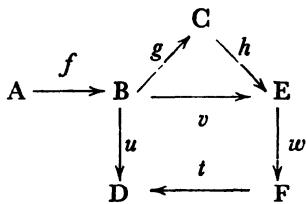
\includegraphics[keepaspectratio]{images/part003_3866b0bf02291d28d06ad2c75d3a73e7be589c55410c746bfd40818492cdc992.jpg}}

其中箭头旁标注的字母表示从箭头尾部集合到箭头头部集合的映射。

映射f=g（即E到F的映射相等）这一关系等价于“对所有 \(x \in E, f(x) = g(x)\) ''.

\begin{enumerate}
\def\labelenumi{\arabic{enumi}.}
\setcounter{enumi}{2}
\tightlist
\item
  定义在集合E上的函数，若对E中的每一个元素x都取相同的值a，则称为E上的常值函数；它由函数关系y = a确定。
\end{enumerate}

将E映入E的映射，它把E中的每个元素x与这个元素本身对应起来，称为恒等映射。它由函数关系y = x确定。

如果A是E的任意子集，则将A中每个元素x视为E中的同一元素而把A映入E的映射，称为A到E的典范映射。

让 \(f\) 是集合 \(\mathbf{E}\) 到自身的一个映射。一个元素 \(x\) （属于 \(\mathbf{E}\) ）被称为在 \(f\) 之下固定（或不变），如果 \(f(x) = x\) .

E 的元素 x 被称为在 E 到 E 的一组映射下固定（或不变），如果它在每个映射下都是固定的。

\begin{enumerate}
\def\labelenumi{\arabic{enumi}.}
\setcounter{enumi}{3}
\tightlist
\item
  让 \(f\) 是从 \(\mathbf{E}\) 到 \(\mathbf{F}\) 的映射，并令 \(\mathbf{X}\) 是 \(\mathbf{E}\) 的任意子集。则 \(\mathbf{X}\) 在 \(f\) 之下的像 \(\mathbf{Y}\) 是 \(\mathbf{F}\) 的一个子集 ，由所有元素 \(y\) （具有性质“存在 \(x \in \mathbf{E}\) 使得 \(x \in \mathbf{X}\) 并且 \(f(x) = y\)”）组成.
\end{enumerate}

这定义了X与Y之间的一种关系，该关系在Y上是函数性的，因此确定了从 \(\mathfrak{P}(\mathbf{E})\) 到 \(\mathfrak{P}(\mathbf{F})\) 的某个映射。该映射被称为 f 到子集集合的典范扩张；为简便起见，它也被记为f，我们写作 \(\mathbf{Y}=f(\mathbf{X})\) .

对于所有 \(f\) 并且 \(x\) 我们拥有

\[
f (\phi) = \phi \quad \text { 且 } \quad f (\{x \}) = \{f (x) \}.
\]

借用语言习惯，值 \(f(x)\) （ \(f\) 在 \(x\) 处的值）也被称为 \(x\) 在 \(f\) 之下的像.

如果 y 是 F 的一般元素，则性质“ \(y \in f(E)\) '' 可以表述为“y 具有以下形式 \(f(x)\) ''.

滥用语言，该像 \(f(\mathbf{E})\) （即 \(\mathbf{E}\) 在 \(f\) 之下的像）有时被称为 \(f\) 的像.

如果我们有 \(f(\mathbf{E}) = \mathbf{F}\) ，即如果对所有 \(y \in \mathbf{F}\) 存在 \(x \in \mathbf{E}\) 使得 \(y = f(x)\) ，那么 \(f\) 被称为从 \(\mathbf{E}\) 到 \(\mathbf{F}\) 上的映射，或满射映射，或满射。

让 \(x\) 是任意元素且 \(X\) 是 \(E\) 的任何子集。我们不说 \(f(x)\) 是 \(f\) 在 \(x\) 处的值、且 \(f(X)\) 是 \(X\) 在 \(f\) 之下的像，而是有时说 \(f\) 把 \(x\) 变换（或映射）为 \(f(x)\) ，把 \(X\) 变换为 \(f(X)\) ; \(f(x)\) 和 \(f(X)\) 则分别称为由 \(f\) 所给出的 \(x\) 和 \(X\) 的变换。

如果 f 是 E 到自身的一个映射，则称 E 的子集 X 在 f 下稳定，如果 \(f(\mathbf{X}) \subset \mathbf{X}\) 。如果 X 在 E 到 E 的映射集合中的每一个映射下都稳定，则称子集 X 在该映射集合下稳定。

\begin{enumerate}
\def\labelenumi{\arabic{enumi}.}
\setcounter{enumi}{4}
\tightlist
\item
  设 \(f\) 是从 \(\mathbf{E}\) 到 \(\mathbf{F}\) 的映射。于是我们有以下命题，其中 \(\mathbf{X}\) 和 \(\mathbf{Y}\) 表示 \(\mathbf{E}\) 的任意子集:
\end{enumerate}

\begin{enumerate}
\def\labelenumi{(\alph{enumi})}
\item
  关系 \(\mathbf{X} \subset \mathbf{Y}\) 蕴含 \(f(\mathbf{X}) \subset f(\mathbf{Y})\) .
\item
  该性质 \(\mathbf{X} \neq \emptyset\) 等价于 \(f(\mathbf{X}) \neq \emptyset\) .
\item
  对于所有 \(\tilde{\mathbf{X}}\) , \(\mathbf{Y}\) 我们拥有
\end{enumerate}

\begin{enumerate}
\def\labelenumi{(\arabic{enumi})}
\setcounter{enumi}{10}
\tightlist
\item
\end{enumerate}

\[
f (\mathbf {X} \cup \mathbf {Y}) = f (\mathbf {X}) \cup f (\mathbf {Y}),\tag{12}
\]

\[
f (\mathbf {X} \cap \mathbf {Y}) \subset f (\mathbf {X}) \cap f (\mathbf {Y}).
\]

\begin{enumerate}
\def\labelenumi{\arabic{enumi}.}
\setcounter{enumi}{5}
\tightlist
\item
  让 \(f\) 是从 \(\mathbf{E}\) 到 \(\mathbf{F}\) 的映射，并且让 \(\mathbf{Y}\) 是 \(\mathbf{F}\) 的任意子集。 \(\mathbf{Y}\) 在 \(f\) 之下的逆像 \(\mathbf{X}\) 是 \(\mathbf{E}\) 的一个子集 ，由所有元素 \(x\) （具有该性质 \(f(x) \in \mathbf{Y}\) ）组成.
\end{enumerate}

这定义了X与Y之间的一种关系，该关系在X上是函数性的，因此确定了从 \(\mathfrak{P}(\mathbf{F})\) 到 \(\mathfrak{P}(\mathbf{E})\) 的一个映射，称为 f 到子集集合上的逆扩张，并记作 \(\overline{f}^{1}\) ；因此我们写 \(\mathbf{X} = \overline{f}^{1}(\mathbf{Y})\) .

特别地，如果 \(y\) 是 \(F\) ，那么 \(f^{1}(\{y\})\) 将是所有 \(x \in E\) 使得 \(f(x) = y\) 。关系“ \(f(x) = y\) ”和“ \(x \in \overline{f}^{1}(\{y\})\) ”是等价的。借用语言习惯，我们常写 \(\overline{f}^{1}(y)\) 以代替 \(\overline{f}^{1}(\{y\})\) .

迹 \(X_{A}\) 子集X在E中对给定子集A的逆像是X在A到E的典范映射（第3节）下的原像。

\begin{enumerate}
\def\labelenumi{\arabic{enumi}.}
\setcounter{enumi}{6}
\tightlist
\item
  让 \(f\) 是从 \(\mathbf{E}\) 到 \(\mathbf{F}\) 的映射。于是我们有以下命题，其中 \(\mathbf{X}\) 和 \(\mathbf{Y}\) 表示 \(\mathbf{F}\) 的任意子集:
\end{enumerate}

\begin{enumerate}
\def\labelenumi{(\alph{enumi})}
\item
  关系 \(\mathbf{X} \subset \mathbf{Y}\) 蕴含 \(\overline{f}^1(\mathbf{X}) \subset \overline{f}^1(\mathbf{Y})\) .
\item
  对所有 X, Y，我们有
\end{enumerate}

\begin{enumerate}
\def\labelenumi{(\arabic{enumi})}
\setcounter{enumi}{12}
\tightlist
\item
\end{enumerate}

\[
\overline {{f}} ^ {1} (\mathrm{X} \cup \mathrm{Y}) = \overline {{f}} ^ {1} (\mathrm{X}) \cup \overline {{f}} ^ {1} (\mathrm{Y}),\tag{14}
\]

\[
\bar {f} ^ {1} (\mathrm{X} \cap \mathrm{Y}) = \bar {f} ^ {1} (\mathrm{X}) \cap \bar {f} ^ {1} (\mathrm{Y}),\tag{15}
\]

\[
\overline {{f}} ^ {1} (\mathbb {C X}) = \mathbb {C} \overline {{f}} ^ {1} (\mathbf {X}).
\]

注意公式(12)与(14)之间的区别；若将f替换为从F到E的任意映射，则(14)并非对所有X和Y都成立。同样，对于任意映射的扩张，不存在与(15)类似的结论。

此外，我们有 \(\overline{f}^{1}(\phi) = \phi\) ；但我们也可以有 \(\overline{f}^{1}(\mathbf{X}) = \phi\) ，其中 \(\mathbf{X}\) 是 \(\mathbf{F}\) 的一个非空子集. 为了使得 \(\mathbf{X} \neq \phi\) 蕴含 \(\overline{f}^{1}(\mathbf{X}) \neq \phi\) ，其充要条件是 \(f\) 是从 \(\mathbf{E}\) 到 \(\mathbf{F}\) 上的映射.

\begin{enumerate}
\def\labelenumi{\arabic{enumi}.}
\setcounter{enumi}{7}
\tightlist
\item
  如果映射 \(f\) （从 \(\mathbf{E}\) 到 \(\mathbf{F}\) 内的）满足对于所有 \(y \in \mathbf{F}\) 至多存在一个 \(x \in \mathbf{E}\) 使得 \(y = f(x)\) （换句话说，集合 \(\overline{f}^1(y)\) 要么为空，要么只包含一个元素），则 \(f\) 被称为从 \(\mathbf{E}\) 到 \(\mathbf{F}\) 内的一一映射，或单射映射，或单射。此时，对于所有子集 \(\mathbf{X}, \mathbf{Y}\) （ \(\mathbf{E}\) 的）,
\end{enumerate}

\[
f (\mathbf {X} \cap \mathbf {Y}) = f (\mathbf {X}) \cap f (\mathbf {Y}).\tag{16}
\]

\begin{enumerate}
\def\labelenumi{\arabic{enumi}.}
\setcounter{enumi}{8}
\tightlist
\item
  如果映射 \(f\) （从 \(\mathbf{E}\) 到 \(\mathbf{F}\) 内的）满足对于所有 \(y \in \mathbf{F}\) 恰好存在一个 \(x \in \mathbf{E}\) 使得 \(y = f(x)\) （换言之， \(\overline{f}(y)\) 由单一元素组成），则 \(f\) 被称为从 \(\mathbf{E}\) 到 \(\mathbf{F}\) 上的一一映射，或双射映射，或双射。这样的映射可以刻画为既是E到F上的映射，又是E到F内的一一映射。
\end{enumerate}

如果 \(f\) 是 \(\mathbf{E}\) 到 \(\mathbf{F}\) 上的一一映射，关系 \(y = f(x)\) 不仅在 \(y\) 中是泛函的，而且在 \(x\) 中也是泛函的。作为 \(x\) 中的泛函关系，它确定了 \(\mathbf{F}\) 到 \(\mathbf{E}\) 上的一个一一映射，称为映射 \(f\) 的逆映射.

注意，f 的逆的延拓与 f 的延拓的逆是相同的。

令 \(g\) 为 \(f\) 的逆。那么关系“ \(y = f(x)\) ”和“ \(x = g(y)\) '' 是等价的。\(g\) 的逆是 \(f\) 。如果 \(f\) 是 \(E\) 到 \(F\) 上的一一映射，我们不仅有关系式 (16)，而且对所有子集 \(X\) （ \(E\) 的）有

\[
f (\mathbf {C X}) = \mathbf {C} f (\mathbf {X}).
\]

此外， \(f\) 的扩张是 \(\mathfrak{P}(\mathbf{E})\) 到 \(\mathfrak{P}(\mathbf{F})\) 上的一一映射.

E到F的一一映射，连同其逆映射，称为实现E与F之间的一一对应；或者说，E与F通过这些映射被置于一一对应之中。

集合E到自身的一一映射称为E的一个置换。恒等映射是一个置换。若一个置换与其逆置换相同，则称其为对合的；例如，映射 \(X \rightarrow C X\) （ \(\mathfrak{P}(E)\) 到自身上的映射）是对合的。

\begin{enumerate}
\def\labelenumi{\arabic{enumi}.}
\setcounter{enumi}{9}
\tightlist
\item
  在以下命题中，X表示E的任意子集，Y表示F的任意子集：
\end{enumerate}

\begin{enumerate}
\def\labelenumi{(\alph{enumi})}
\tightlist
\item
  如果 \(f\) 是从 \(\mathbf{E}\) 到 \(\mathbf{F}\) 的映射，我们有
\end{enumerate}

\begin{enumerate}
\def\labelenumi{(\arabic{enumi})}
\setcounter{enumi}{16}
\tightlist
\item
\end{enumerate}

\[
\overline {{{f}}} ^ {1} (\mathrm{Y}) = \overline {{{f}}} ^ {1} (\mathrm{Y} \cap f (\mathrm{E})),\tag{18}
\]

\[
\mathbf {X} \subset \overline {{f}} ^ {1} (f (\mathbf {X})),\tag{19}
\]

\[
f (\overline {{f}} ^ {1} (\mathbf {Y})) \subset \mathbf {Y}.
\]

\begin{enumerate}
\def\labelenumi{(\alph{enumi})}
\setcounter{enumi}{1}
\item
  性质“对于所有Y， \(f(\bar{f}^{1}(Y)) = Y\) “f是E到F上的映射”与“f是E到F的满射”是等价的。
\item
  所有X都具有的性质， \(\overline{f}^{1}(f(X)) = X\) “f是E到F的一一映射”与“f是E到F的单射”是等价的。
\item
  对所有X和Y，
\end{enumerate}

\[
\bar {f} ^ {1} (f (\mathbf {X})) = \mathbf {X} \quad \text { 且 } \quad f (\bar {f} ^ {1} (\mathbf {Y})) = \mathbf {Y}"
\]

且“f是E到F上的一一映射”是等价的。

\begin{enumerate}
\def\labelenumi{\arabic{enumi}.}
\setcounter{enumi}{10}
\tightlist
\item
  设E、F、G为三个集合，它们可能相同也可能不同。设f为从E到F的映射，g为从F到G的映射。从E到G的映射，其在E中任一元素x处的值为 \(g(f(x))\) 称为g与f的复合，记作 \(g \circ f\) ，或在无歧义时简记为gf。
\end{enumerate}

这个等式 \(h = g \circ f\) 被称为 h 的一个分解。

注意，如果 G 与 E 不同，我们可能不能谈论 f 和 g 的复合（按此顺序），并且记号 \(f \circ g\) 没有意义。如果 G 与 E 相同，则 \(f \circ g\) 并且 \(g \circ f\) 不属于同一个集合，除非F也与E相同；即使如此，通常也是 \(f \circ g \neq g \circ f\) 。因此f和g的复合顺序是至关重要的。

令 \(\varphi\) 为 \(g\) 与 \(f\) 的复合，令 \(\mathbf{X}\) 是 \(\mathbf{E}\) 的任意子集，并且令 \(\mathbf{Z}\) 是 \(\mathbf{G}\) 的任意子集。于是我们有

\begin{enumerate}
\def\labelenumi{(\arabic{enumi})}
\setcounter{enumi}{19}
\tightlist
\item
\end{enumerate}

\[
\varphi (\mathbf {X}) = g (f (\mathbf {X})),\tag{21}
\]

\[
\overline {{{\varphi}}} ^ {1} (Z) = \overline {{{f}}} ^ {1} (\overline {{{g}}} ^ {1} (Z)).
\]

如果 \(f\) 是 \(\mathbf{E}\) 到 \(\mathbf{F}\) 上的一一映射，并且如果 \(g\) 是 \(\mathbf{F}\) 到 \(\mathbf{G}\) 上的一一映射，那么 \(g \circ f\) 是 \(\mathbf{E}\) 到 \(\mathbf{G}\) 上的一一映射.

让 \(h\) 是从 \(G\) 到一个集合 \(H\) 的映射。于是我们有

\[
h \circ (g \circ f) = (h \circ g) \circ f;
\]

的复合，这个从E到H的映射写作 \(h \circ g \circ f\) ，并称为三个映射 h、g、f 按此顺序的复合。多于三个映射的复合类似地定义。

如果 \(f\) 是 \(\mathbf{E}\) 到自身的映射，其迭代 \(f\) 被定义为映射 \(f^n\) ( \(n\) 为整数 \(\geqslant 1\) )（即 \(\mathbf{E}\) 到自身的映射），通过对 \(n\) 的归纳、借助于关系 \(f^1 = f\) , \(f^n = f^{n-1} \circ f\) 来定义； \(f^n\) 被称为 \(f\) 的n次迭代。我们有 \(f^{m+n} = f^m \circ f^n\) .

\begin{enumerate}
\def\labelenumi{\arabic{enumi}.}
\setcounter{enumi}{11}
\tightlist
\item
  一般来说，复合映射 \(\overline{f}^{1} \circ f\) （由一个映射 \(f\) 的逆扩张与扩张复合而成）并不是 \(\mathfrak{P}(\mathbf{E})\) 到自身的恒等映射。同样地， \(f \circ \overline{f}^1\) 通常也不是 \(\mathfrak{P}(\mathbf{E})\) 到自身的恒等映射。这两个条件同时成立，仅当 \(f\) 是 \(\mathbf{E}\) 到 \(\mathbf{F}\) 上的双射.
\end{enumerate}

如果 \(f\) 是 \(\mathbf{E}\) 到 \(\mathbf{F}\) 上的双射，并且如果 \(g\) 表示 \(f\) 的逆，则复合 \(g \circ f\) 与 \(f \circ g\) 分别是 \(\mathbf{E}\) 到 \(\mathbf{E}\) 上以及 \(\mathbf{F}\) 到 \(\mathbf{F}\) 上的恒等映射.

反之，如果 \(f\) 是从 \(\mathbf{E}\) 到 \(\mathbf{F}\) 的映射，以及 \(g\) 是从 \(\mathbf{F}\) 到 \(\mathbf{E}\) 的映射，使得 \(g \circ f\) 是 \(\mathbf{E}\) 的一个排列并且 \(f \circ g\) 是 \(\mathbf{F}\) 的一个排列，那么 \(f\) 是 \(\mathbf{E}\) 到 \(\mathbf{F}\) 上的双射并且 \(g\) 是 \(\mathbf{F}\) 到 \(\mathbf{E}\) 上的双射.

此外，如果 \(g \circ f\) 是 \(\mathbf{E}\) 到自身上的恒等映射，那么 \(g\) 是 \(f\) 的逆.

\begin{enumerate}
\def\labelenumi{\arabic{enumi}.}
\setcounter{enumi}{12}
\item
  设 \(f\) 是从 \(\mathbf{E}\) 到 \(\mathbf{F}\) 的映射，并设 \(\mathbf{A}\) 是 \(\mathbf{E}\) 的任意子集. 映射 \(f_{\mathbf{A}}\) （由 \(\mathbf{A}\) 到 \(\mathbf{F}\) ，其在任意元素 \(x\) （ \(\mathbf{A}\) 的）处的值为 \(f(x)\) ）称为 \(f\) 在子集 \(\mathbf{A}\) 上的限制；它就是 \(f\) 与由 \(\mathbf{A}\) 到 \(\mathbf{E}\) 的典范映射的复合. 如果两个映射 \(f, g\) （由 \(\mathbf{E}\) 到 \(\mathbf{F}\) ）在 \(\mathbf{A}\) 上的限制相同，则称它们在 \(\mathbf{A}\) 上一致. 反之， \(f\) 称为 \(f_{\mathbf{A}}\) 到 \(\mathbf{E}\) 的扩张.
\item
  将一个集合 E 映到集合 F 上的映射也称为 F 借助 E 的一个参数表示；此时 E 称为该表示的参数集，而 E 的元素则称为参数。
\end{enumerate}

集合 F 的一个元素族，按定义是 F 的一个子集连同其上的一个参数表示；换言之，给定 F 的一个元素族，等价于给定某个集合 E 到 F 的一个映射。E 在该映射下的像称为该族的元素集。注意，F 的两个不同的元素族可能具有相同的 F 的子集作为它们的元素集。

对于集合 F 的每个子集 A，我们总可以联系一个元素族，其元素集为 A。只需考虑由 A 到 F 的典范映射所定义的族即可。

由映射 \(\iota\to x_{i}\) 定义的 F 的元素族，记为 \((x_{i})_{i\in I}\) ，或简称为 \((x_{i})\) 如果关于指标集没有歧义的话。

如果 \(J\) 是 \(I\) 的子集，族 \((x_{t})_{t\in J}\) 被称为对应于 \(J\) 的子族（族 \((x_{t})_{t\in I}\) 的）；它由在 \(J\) 上限制映射 \(t\to x_t\) 而定义.

\section{集合的乘积}

\begin{enumerate}
\def\labelenumi{\arabic{enumi}.}
\tightlist
\item
  设 E, F 是两个集合，它们可以相同也可以不同。有序对 \((x, y)\) ，其中第一个元素 x 是 E 的任意元素，第二个元素 y 是 F 的任意元素，它们构成一个新集合的元素，该集合称为 E 与 F 的乘积，记为 \(E \times F\) ；E 和 F 称为 \(E \times F\) 的因子。两个有序对被认为相同，仅当它们具有相同的第一个元素和相同的第二个元素；换言之，关系“ \((x, y) = (x', y')\) ''等价于关系`` \(x = x'\) 并且 \(y = y''\) ”。若 z 是 \(E \times F\) 的任意元素，则关系“x 是有序对 \(z''\) 的第一个元素”是 x 的一个函数关系；它确定了一个从 \(E \times F\) 到 E 的映射，称为第一坐标函数，或第一投影，记为 \(pr_{1}\) 。除了说“x 是有序对 \(z''\) 的第一个元素”之外，我们也说“x 是 \(z''\) 的第一坐标（或投影）”或“ \(x = \mathrm{pr}_1z''\) ”。类似地，我们定义第二坐标函数，或第二投影，它是从 \(E \times F\) 到 \(F\) 上的映射，记为 \(\mathrm{pr}_2\) .
\end{enumerate}

关系“ \(x = \text{pr}_1 z\) 并且 \(y = \text{pr}_2 z\) ”等价于“ \(z = (x, y)\) ''.

函数 \(pr_{1}\) 到子集所成集合的扩张，按照一般约定用相同的符号表示，并再次称为第一投影（这里我们不用“坐标”一词）；第二投影的扩张也类似。

\begin{enumerate}
\def\labelenumi{\arabic{enumi}.}
\setcounter{enumi}{1}
\tightlist
\item
  E 的生成元 x 与 F 的生成元 y 之间的关系 R 是有序对 \((x, y)\) 的一个性质，因此定义了乘积 \(E \times F\) 的一个子集，称为 R 的图。反之， \(E \times F\) 的每个子集 A 都是 x 与 y 之间关系“ \((x, y) \in A\) ”的图。
\end{enumerate}

设 A 是 E 的子集，B 是 F 的子集。我们用 \(A \times B\) 表示 \(E \times F\) 的由 x 与 y 之间关系“ \(x \in A\) 并且 \(y \in B\) ”定义的子集。

\begin{enumerate}
\def\labelenumi{\arabic{enumi}.}
\setcounter{enumi}{2}
\tightlist
\item
  在以下命题中，X 和 X' 表示 E 的任意子集，Y 和 Y' 表示 F 的任意子集，Z 表示 E × F 的任意子集。
\end{enumerate}

\begin{enumerate}
\def\labelenumi{(\alph{enumi})}
\item
  关系“X × Y = φ”等价于“X = φ 或 Y = φ”。
\item
  如果 \(X \times Y \neq \emptyset\) ，关系“ \(X \times Y \subset X' \times Y''\) ”等价于“ \(X \subset X'\) 并且 \(Y \subset Y''\) ''.
\item
  对于所有 \(\mathbf{X},\mathbf{X}^{\prime},\mathbf{Y}\) 我们拥有
\end{enumerate}

\[
(\mathbf {X} \times \mathbf {Y}) \cup (\mathbf {X} ^ {\prime} \times \mathbf {Y}) = (\mathbf {X} \cup \mathbf {X} ^ {\prime}) \times \mathbf {Y}.\tag{22}
\]

\begin{enumerate}
\def\labelenumi{(\alph{enumi})}
\setcounter{enumi}{3}
\tightlist
\item
  对于所有 \(\mathbf{X},\mathbf{X}^{\prime},\mathbf{Y},\mathbf{Y}^{\prime}\) 我们拥有
\end{enumerate}

\[
(\mathbf {X} \times \mathbf {Y}) \cap (\mathbf {X} ^ {\prime} \times \mathbf {Y} ^ {\prime}) = (\mathbf {X} \cap \mathbf {X} ^ {\prime}) \times (\mathbf {Y} \cap \mathbf {Y} ^ {\prime}).
\]

\begin{enumerate}
\def\labelenumi{(\alph{enumi})}
\setcounter{enumi}{4}
\tightlist
\item
  对所有 X, Y，我们有
\end{enumerate}

\[
\mathrm{pr} _ {1} ^ {- 1} (\mathbf {X}) = \mathbf {X} \times \mathbf {F}, \quad \mathrm{pr} _ {2} ^ {- 1} (\mathbf {Y}) = \mathbf {E} \times \mathbf {Y}.\tag{24}
\]

\begin{enumerate}
\def\labelenumi{(\alph{enumi})}
\setcounter{enumi}{5}
\tightlist
\item
  如果 \(\mathbf{Y} \neq \emptyset\) ，那么对所有 \(\mathbf{X}\) 我们拥有
\end{enumerate}

\[
\operatorname{pr} _ {1} (\mathbf {X} \times \mathbf {Y}) = \mathbf {X}.\tag{25}
\]

\begin{enumerate}
\def\labelenumi{(\alph{enumi})}
\setcounter{enumi}{6}
\tightlist
\item
  对所有 Z，我们有
\end{enumerate}

\[
Z \subset \operatorname{pr} _ {1} (Z) \times \operatorname{pr} _ {2} (Z).\tag{26}
\]

\begin{enumerate}
\def\labelenumi{(\alph{enumi})}
\setcounter{enumi}{7}
\tightlist
\item
  令 \(a\) 为 \(\mathbf{E}\) 的一个元素。则映射 \((a, y) \to y\) （集合 \(\{a\} \times \mathbf{F}\) 到 \(\mathbf{F}\) 上的，即 \(\mathbf{pr}_2\) 到子集 \(\{a\} \times \mathbf{F}\) 的限制）是一对一的。
\end{enumerate}

\begin{enumerate}
\def\labelenumi{\arabic{enumi}.}
\setcounter{enumi}{3}
\item
  该映射

\[
(x, y) \rightarrow (y, x)\tag{27}
\]

是 \(E \times F\) 到 \(F \times E\) 上的一一映射，并称为典范映射。当 E 和 F 是同一个集合时，映射 (27) 称为典范对称；它此时是对合的。元素 \((x, y)\) （属于 \(E \times E\) ）在此对称下保持不变的，正是那些具有性质 x = y 的元素；这些元素组成的集合 \(\Delta\) 称为 \(E \times E\) 的对角线. 映射 \(x \to (x, x)\) 是 E 到 \(\Delta\) 上的双射，称为 E 到 \(E \times E\) 中的对角映射.

如果 Z 是 \(E \times F\) 的任意子集，Z 在 \(E \times F\) 到 \(F \times E\) 上的典范映射下的像记作 \(\overline{Z}^{1}\) . 如果 X 是 E 的任意子集且 Y 是 F 的任意子集，则

\[
\overline{\mathbf {X} \times \mathbf {Y}}^{1} = \mathbf {Y} \times \mathbf {X}.
\]

如果 x 与 y 之间的关系 R，作为有序对 \((x, y)\) 的一个性质，定义了 \(E \times F\) 的一个子集 A，那么同一关系，作为该对的一个性质 \((y, x)\) ，定义子集 \(\overline{A}^{1}\) 的 \(F \times E\) 。R 等价于以下每个关系 \((x, y) \in A\) , \((y, x) \in \overline{A}^{1}\) 。如果 E 和 F 是同一个集合，则当 \(A = \overline{A}^{1}\) 时，关系 R 及相应的子集 A 被称为对称的。对角线 \(\Delta\) （由相等关系定义的）是对称的。如果 Z 是 \(E \times E\) ，那么 \(Z \cup \overline{Z}^{1}\) 并且 \(Z \cap \overline{Z}^{1}\) 是对称的。

\end{enumerate}

\begin{enumerate}
\def\labelenumi{\arabic{enumi}.}
\setcounter{enumi}{4}
\tightlist
\item
  设A是集合E的一个子集，且f是从A到集合F的一个映射。关系“ \(x \in A\) 并且 \(y = f(x)\) '' 在 E 的任意元素 x 与 F 的任意元素 y 之间定义了一个子集，该子集属于 \(E \times F\) 称为函数 f 的图像。～若 B 是 E 中包含 A 的子集，且 g 是 f 到 B 的延拓（§ 2，第 13 号），则 f 的图像包含于 g 的图像中。
\end{enumerate}

反之，设 C 是 \(\mathbf{E} \times \mathbf{F}\) 的一个子集，使得对于每个 \(x \in \mathbf{E}\) ，至多存在一个 \(y \in \mathbf{F}\) 使得 \((x, y) \in \mathbf{C}\) 。则关系 \((x, y) \in \mathbf{C}\) （在一般元素 \(x\) （属于集合 \(\operatorname{pr}_1(\mathbf{C})\) ）与一个一般元素 \(y\) （属于 \(\mathbf{F}\) ）之间）是 \(y\) 中的函数关系，并确定 \(\operatorname{pr}_1(\mathbf{C})\) 到 \(\mathbf{F}\) 中的一个映射，其图像为 \(\mathbf{C}\) .

子集 C 的集合， \(E \times F\) 其具有性质“对所有 \(x \in E\) 至多存在一个 \(y \in F\) 使得 \((x, y) \in C\) ''（一个集合，它是 \(\mathfrak{P}(\mathbf{E} \times \mathbf{F})\) 因此可以与将E的子集映射到F的映射集合建立一一对应关系。

让 \(f\) 是从 \(\mathbf{E}\) 到 \(\mathbf{F}\) 的单射映射，并且让 \(g\) 是 \(f\) （视为 \(\mathbf{E}\) 到 \(f(\mathbf{E})\) 上的双射）的逆。如果 \(\mathbf{C}\) 是 \(f\) 的图像，则 \(g\) 的图像是 \(\overline{\mathbf{C}}^1\) .

\begin{enumerate}
\def\labelenumi{\arabic{enumi}.}
\setcounter{enumi}{5}
\tightlist
\item
  如果 \(f\) 是从 \(\mathbf{E}\) 到 \(\mathbf{F}\) 的映射，以及 \(\mathbf{C}\) 是其在 \(\mathbf{E} \times \mathbf{F}\) 中的图像，关系“ \(y = f(x)\) ”等价于“ \((x, y) \in \mathbf{C}\) ''。关系“ \(y \in f(\mathbf{X})\) '' 等价于“存在 \(x\) 使得 \(x \in \mathbf{X}\) 并且 \((x, y) \in \mathbf{C}\) ''.
\end{enumerate}

现在设K是E×F的任意子集，X是E的任意子集。用K(X)表示F中由所有满足关系“存在x使得 \(x \in X\) 并且 \((x, y) \in K\) ''”的元素y组成的子集；因此该关系等价于`` \(y \in K(X)\) ''。映射 \(X \to K(X)\) （从 \(\mathfrak{P}(E)\) 到 \(\mathfrak{P}(F)\) 的）称为由E × F的子集K所定义。注意，K(X)是集合 \(K \cap (X \times F)\) 的第二投影。如果 K 是映射 f 从 E 到 F 的图像，那么该映射 \(X \to K(X)\) 是 f 到子集集合的典范扩张。

\begin{enumerate}
\def\labelenumi{\arabic{enumi}.}
\setcounter{enumi}{6}
\tightlist
\item
  如果 \(x\) 是 \(\mathbf{E}\) 的典型元素，那么 \(x \to \mathrm{K}(\{x\})\) 是从 \(\mathbf{E}\) 到 \(\mathfrak{P}(\mathbf{F})\) 的映射，其值 \(\mathrm{K}(\{x\})\) （为简便起见也记为 \(\mathrm{K}(x)\) ）称为 \(\mathbf{K}\) 在 \(x\) 处的截面。关系 \((x, y) \in \mathbf{K}\) 等价于 \(y \in \mathrm{K}(x)\) .
\end{enumerate}

反之，每个映射 \(x \to \Phi(x)\) （从 \(E\) 到 \(\mathfrak{P}(F)\) ）可以以这种方式获得；因为该关系 \(y \in \Phi(x)\) 定义了子集 \(K\) （ \(E \times F\) 的），以及 \(\Phi(x)\) 正是 \(K\) 在 \(x\) 处的截面。集合 \(\mathfrak{P}(E \times F)\) 以及 \(E\) 到 \(\mathfrak{P}(F)\) 的映射的集合因此是一一对应的。

\begin{enumerate}
\def\labelenumi{\arabic{enumi}.}
\setcounter{enumi}{7}
\tightlist
\item
  每个映射 \(\mathbf{X} \to \mathbf{K}(\mathbf{X})\) （由子集 \(\mathbf{K}\) （ \(\mathbf{E} \times \mathbf{F}\) 的）所定义的）具有以下性质，这些性质推广了从 \(\mathbf{E}\) 到 \(\mathbf{F}\) 的映射的典范扩张的性质 (§2，第4和第5条)：
\end{enumerate}

\begin{enumerate}
\def\labelenumi{(\alph{enumi})}
\item
  \(\mathbf{K}(\phi)=\phi.\)
\item
  “X ⊂ Y” 蕴含 “K(X) ⊂ K(Y)”。
\item
  对所有 X, Y，我们有
\end{enumerate}

\begin{enumerate}
\def\labelenumi{(\arabic{enumi})}
\setcounter{enumi}{27}
\tightlist
\item
\end{enumerate}

\[
\mathbf {K} (\mathbf {X} \cup \mathbf {Y}) = \mathbf {K} (\mathbf {X}) \cup \mathbf {K} (\mathbf {Y}),\tag{29}
\]

\[
\mathbf {K} (\mathbf {X} \cap \mathbf {Y}) \subset \mathbf {K} (\mathbf {X}) \cap \mathbf {K} (\mathbf {Y}).
\]

若 K 且 \(K'\) 是 \(E \times F\) 使得 \(K \subset K'\) ，那么我们有 \(\mathrm{K}(\mathrm{X}) \subset \mathrm{K}'(\mathrm{X})\) 对于所有 \(X \subset E\) ；特别地， \(\mathrm{K}(x) \subset \mathrm{K}'(x)\) 对于所有 \(x \in E\) 。反之，若 \(\mathrm{K}(x) \subset \mathrm{K}'(x)\) 对于所有 \(x \in E\) ，那么 \(K \subset K'\) .

\begin{enumerate}
\def\labelenumi{\arabic{enumi}.}
\setcounter{enumi}{8}
\tightlist
\item
  E 的一般元素与 F 的一般元素之间的关系定义了 \(E \times F\) 的一个子集 K 以及 \(\overline{K}\) （ \(F \times E\) 的一个子集），因此有映射 \(X \to K(X)\) （从 \(\mathfrak{P}(E)\) 到 \(\mathfrak{P}(F)\) ）以及一个映射 \(Y \to \overline{K}(Y)\) （从 \(\mathfrak{P}(F)\) 到 \(\mathfrak{P}(E)\) ).
\end{enumerate}

如果 \(\mathbf{K}\) 是某个映射 \(f\) （从 \(\mathbf{E}\) 到 \(\mathbf{F}\) 的）的图像，映射 \(\mathbf{Y} \to \overline{\mathbf{K}}(\mathbf{Y})\) 是 \(f\) 的逆扩张.

应当注意，关系式(18)和(19)并不推广到映射 \(\mathbf{X} \to \mathbf{K}(\mathbf{X})\) 并且 \(\mathbf{Y} \to \overline{\mathbf{K}}^{1}(\mathbf{Y})\) ，当 \(\mathbf{K}\) 是 \(\mathbf{E} \times \mathbf{F}\) 的任意子集时.

\begin{enumerate}
\def\labelenumi{\arabic{enumi}.}
\setcounter{enumi}{9}
\tightlist
\item
  设E、F、G为三个集合，它们可能相同也可能不同，设A为 \(E \times F\) 的子集，并令 B 为 \(F \times G\) 的子集。则元素 \((x, z)\) （属于 \(E \times G\) ）中具有性质“存在 \(y \in F\) 使得 \((x, y) \in A\) 并且 \((y, z) \in B\) '' 的那些构成 \(E \times G\) 的一个子集，称为B与A的复合，记作 \(B \circ A\) ，或在无混淆风险时简称为BA。这里再次强调，复合的顺序至关重要。¶ 映射 \(X \to BA(X)\) （从 \(\mathfrak{P}(E)\) 到 \(\mathfrak{P}(G)\) ）是 \(Y \to B(Y)\) 与 \(X \to A(X)\) 的复合；换言之，对所有 \(X \subset E\) 我们拥有
\end{enumerate}

\[
\mathbf {B A} (\mathbf {X}) = \mathbf {B} (\mathbf {A} (\mathbf {X})).\tag{30}
\]

设H为另一个集合，不一定与E、F、G不同，并设C为 \(G \times H\) 的一个子集。于是我们有 \(\mathbf{C} \circ (\mathbf{B} \circ \mathbf{A}) = (\mathbf{C} \circ \mathbf{B}) \circ \mathbf{A}\) ；该集合也记作 \(C \circ B \circ A\) （或简记为CBA），并称为C、B、A按此顺序的复合。

让 \(f\) 是从 \(\mathbf{E}\) 到 \(\mathbf{F}\) 的映射，并且让 \(g\) 是从 \(\mathbf{F}\) 到 \(\mathbf{G}\) 的映射。如果 \(\mathbf{A}\) （相应地 \(\mathbf{B}\) ）是 \(f\) （相应地 \(g\) ）的图像，则复合 BA 是复合映射 \(g \circ f\) 的图像.

\begin{enumerate}
\def\labelenumi{\arabic{enumi}.}
\setcounter{enumi}{10}
\tightlist
\item
  我们有
\end{enumerate}

\[
\overline{\mathbf {B} \circ \mathbf {A}}^{1} = \overline {\mathbf {A}}^{1} \circ \overline {\mathbf {B}}^{1}.\tag{31}
\]

设 A, A' 是 E × F 的两个子集，设 B, B' 是 F × G 的两个子集。则关系

\[
" \mathbf {A} \subset \mathbf {A} ^ {\prime} \text {   且   } \mathbf {B} \subset \mathbf {B} ^ {\prime}" \quad \text { 蕴含 } \quad " \mathbf {B} \circ \mathbf {A} \subset \mathbf {B} ^ {\prime} \circ \mathbf {A} ^ {\prime}".
\]

设 A 是 \(E \times F\) 的子集， \(\Delta\) 为 \(E \times E\) 的对角线，以及 \(\Delta'\) 为 \(F \times F\) 的对角线。于是我们有

\[
\mathbf {A} \circ \Delta = \Delta^ {\prime} \circ \mathbf {A} = \mathbf {A}.\tag{32}
\]

\begin{enumerate}
\def\labelenumi{\arabic{enumi}.}
\setcounter{enumi}{11}
\tightlist
\item
  设E、F、G为三个集合，它们可能相同也可能不同。它们的积 \(E \times F \times G\) 是三元有序组的集合 \((x, y, z)\) ，其中 \(x \in E\) , \(y \in F\) ，以及 \(z \in G\) ，关系“ \((x, y, z) = (x', y', z')\) '' 等价于 `` \(x = x'\) 并且 \(y = y'\) 并且 \(z = z''\) ''。这三个映射 \((x, y, z) \to x\) , \((x, y, z) \to y\) , \((x, y, z) \to z\) （从 \(E \times F \times G\) 分别到E、F、G上）被称为第一、第二和第三坐标函数（或投影）；类似地，例如，指标为1、2的投影是映射
\end{enumerate}

\[
(x, y, z) \rightarrow (x, y)
\]

（ \(\mathbf{E} \times \mathbf{F} \times \mathbf{G}\) 到 \(\mathbf{E} \times \mathbf{F}\) 上的），并记作 \(\mathbf{pr}_{1,2}\) .

第2、3、4号的定义和命题很容易推广到三个集合的乘积。

此外，与其考虑三个集合的乘积 \(E \times F \times G\) ，我们同样可以考虑乘积 \((\mathbf{E} \times \mathbf{F}) \times \mathbf{G}\) ，它由对两个集合作乘积这一运算的两次应用而得到。事实上， \((x, y, z) \to ((x, y), z)\) 是 \(E \times F \times G\) 到 \((\mathbf{E} \times \mathbf{F}) \times \mathbf{G}\) 上的一个一一映射，称为典范的。类似地，我们定义 \(E \times F \times G\) 到集合 \(E \times (F \times G)\) 上的一一映射，以及到所有由 \(E \times F \times G\) , \((\mathbf{E} \times \mathbf{F}) \times \mathbf{G}\) ，以及 \(E \times (F \times G)\) 通过置换三个字母E、F、G而得到的集合上的一一映射。

对于三个以上集合的乘积，也有类似的定义和性质。

\begin{enumerate}
\def\labelenumi{\arabic{enumi}.}
\setcounter{enumi}{12}
\tightlist
\item
  如果一个函数 \(f\) ，其取值在任意集合 \(\mathbf{E}'\) 中，定义在三个集合的乘积 \(\mathbf{E}\) , \(\mathbf{F}\) , \(\mathbf{G}\) 上，则称它为三变量函数，其中每个变量分别遍历其中一个集合 \(\mathbf{E}\) , \(\mathbf{F}\) , \(\mathbf{G}\) 的值 \(f\) 在元素 \((x, y, z)\) 的 \(\mathbf{E} \times \mathbf{F} \times \mathbf{G}\) 处记作 \(f(x, y, z)\) .
\end{enumerate}

让 \(a\) 为 \(\mathbf{E}\) 的任意元素。则 \((y, z) \to f(a, y, z)\) 是从 \(\mathbf{F} \times \mathbf{G}\) 到 \(\mathbf{E}'\) 的映射，称为由 \(f\) 确定的部分映射（或函数），对应于该值 \(a\) （ \(x\) 所取的）；它也是 \(f\) 与映射 \((y, z) \to (a, y, z)\) （从 \(\mathbf{F} \times \mathbf{G}\) 到 \(\mathbf{E} \times \mathbf{F} \times \mathbf{G}\) ）的复合.

类似地，如果 \(b\) 是 \(\mathbf{F}\) 的一个元素，那么 \(z \to f(a, b, z)\) 是从 \(\mathbf{G}\) 到 \(\mathbf{E}'\) 的一个映射，称为由 \(f\) 确定的部分映射，对应于值 \(a, b\) （ \(x, y\) 所取的）.

反之，设g为从E到 \(E'\) 的映射。则 \((x, y, z) \to g(x)\) 是 \(E \times F \times G\) 到 \(E'\) 的一个映射 h，使得由 h 决定的、E 到 \(E'\) 的部分映射（对应于 y 和 z 的任何值）都与 g 相同。这一事实通常表述为：关于自变量 x 的函数总可以被视为关于在给定时刻需要考虑的所有自变量（当然包括 x）的函数。

\begin{enumerate}
\def\labelenumi{\arabic{enumi}.}
\setcounter{enumi}{13}
\tightlist
\item
  让 \(f, g, h\) 分别是从 \(\mathbf{E}\) 到 \(\mathbf{E}'\) , 从 \(\mathbf{F}\) 到 \(\mathbf{F}'\) , 从 \(\mathbf{G}\) 到 \(\mathbf{G}'\) 的三个映射。映射 \((x, y, z) \to (f(x), g(y), h(z))\) （从 \(\mathbf{E} \times \mathbf{F} \times \mathbf{G}\) 到 \(\mathbf{E}' \times \mathbf{F}' \times \mathbf{G}'\) ）记作 \((f, g, h)\) 或 \(f \times g \times h\) ，称为 \(f, g, h\) 到乘积的扩张。如果所有三个 \(f, g, h\) 是单射（相应地，满射、双射），则 \(f \times g \times h\) 是单射（相应地，满射、双射）。
\end{enumerate}

在本小节及上一小节中，我们仅考虑三个集合的情形，只是为了明确概念；对于任意有限个集合，类似的讨论同样成立。

\section{集合族的并、交、积}

\begin{enumerate}
\def\labelenumi{\arabic{enumi}.}
\tightlist
\item
  在本节中，我们考虑集合E的子集的一个族 \((\mathbf{X}_{i})_{i\in\mathbf{I}}\) ，其中指标集I是任意的；属于该族的E的子集所构成的集合将记为 \(\mathfrak{F}\) （它因此是 \(\mathfrak{P}(\mathbf{E})\) 的一个子集）.
\end{enumerate}

如果 I 是有限的，那么考虑族 \((\mathbf{X}_{t})\) 归结为E的若干子集的问题，这些子集可能相同也可能不同，其数目等于I的元素个数。例如，E 的任意三个子集 \(X_{1}, X_{2}, X_{3}\) 构成 E 的一个子集族，这里的指标集由数字 1、2、3 组成。

\begin{enumerate}
\def\labelenumi{\arabic{enumi}.}
\setcounter{enumi}{1}
\tightlist
\item
  让 \(J\) 是 \(I\) 的任意子集，并考虑所有元素 \(x\) 组成的集合，这些元素具有性质“存在 \(\iota \in J\) 使得 \(x \in X_\iota\)''。这个集合被称为集合族 \((X_\iota)_{\iota \in J}\) 的并集，并记作 \(\bigcup_{\iota\in J} X_\iota\) .
\end{enumerate}

我们也可以将这一表述定义如下：对于映射 \(\iota \to \mathbf{X}_{\iota}\) （从 \(\mathbf{I}\) 到 \(\mathfrak{P}(\mathbf{E})\) ）对应着一个良定义的子集 \(\mathbf{C}\) （ \(\mathbf{I} \times \mathbf{E}\) 的）使得 \(\mathbf{X}_{\iota} = \mathbf{C}(\iota)\) ( \(\S 3\) ，第7号），并且我们有 \(\bigcup_{\iota \in J} \mathbf{X}_{\iota} = \mathbf{C}(\mathbf{J})\) .

特别是，

\[
\bigcup_ {t \in \varnothing} \mathrm{X} _ {t} = \mathrm{C} (\varnothing) = \varnothing .\tag{33}
\]

当 \(J = I\) ，我们常写作 \(\bigcup_{i} X_i\) ，或简称为 \(\bigcup X_i\) ，代替 \(\bigcup_{i \in I} X_i\) .

并集 \(\bigcup_{i} X_{i}\) 仅依赖于集合 \(\mathfrak{F}\) ；换言之，对于对应于同一子集 \(\mathfrak{F}\) （ \(\mathfrak{P}(E)\) 的）的两个族，它是相同的。特别地，它等于由 \(\mathfrak{F}\) 到 \(\mathfrak{P}(E)\) 的典范映射所定义的族之并，因此我们可以写成 \(\bigcup_{X \in \mathfrak{F}} X\) ，它也称为属于 \(\mathfrak{F}\) 的集合之并.

当 \(\mathbf{I}\) 是一个其元素被明确指定的集合，例如数1、2、3，我们有

\[
\bigcup_ {i \in I} X _ {i} = X _ {1} \cup X _ {2} \cup X _ {3},
\]

这证明了在一般情况下赋予该集合的名称“并”是合理的。 \(\bigcup_{i}X_{i}\) .

\begin{enumerate}
\def\labelenumi{\arabic{enumi}.}
\setcounter{enumi}{2}
\tightlist
\item
  对于任意 \(J \subset I\) 我们拥有
\end{enumerate}

\[
\bigcup_ {i \in J} X _ {i} \subset \bigcup_ {i \in I} X _ {i}.
\]

特别地，对于所有 \(x \in I\) ，我们有

\[
\mathrm{X} _ {x} \subset \bigcup_ {i \in I} \mathrm{X} _ {i}.
\]

反之，如果 Y 是 E 的子集且满足 \(X_{i} \subset Y\) 对于所有 \(i \in I\) ，那么

\[
\bigcup_ {i} \mathrm{X} _ {i} \subset \mathrm{Y}.
\]

更一般地，如果 \((\mathbf{Y}_{i})\) 是E的另一族子集，由同一指标集I索引，并且如果 \(X_{i} \subset Y_{i}\) 对于所有 \(i \in I\) ，那么

\[
\bigcup_ {i} X _ {i} \subset \bigcup_ {i} Y _ {i}.
\]

设 F 为另一个集合，并设 \(\mathbf{X} \to \mathbf{K}(\mathbf{X})\) 为从 \(\mathfrak{P}(\mathbf{E})\) 到 \(\mathfrak{P}(\mathbf{F})\) 的映射，它由 \(E \times F\) 的子集 K 定义。于是我们有

\[
\mathrm{K} \left(\bigcup_ {i \in J} \mathrm{X} _ {i}\right) = \bigcup_ {i \in J} \mathrm{K} (\mathrm{X} _ {i}).\tag{34}
\]

现在令 \(\mathbf{L}\) 为另一个指标集，且 \((J_{\lambda})_{\lambda \in \mathbf{L}}\) 为 \(\mathbf{I}\) 。然后

\[
\bigcup_ {\iota \in \bigcup_ {\lambda \in L} J _ {\lambda}} X _ {\iota} = \bigcup_ {\lambda \in L} \left(\bigcup_ {\iota \in J _ {\lambda}} X _ {\iota}\right).\tag{35}
\]

的子集族。这是并集的一般结合律公式。当 I 和 L 是元素被明确指定的集合时，我们得到的这些关系已经给出（见第 1 节，第 14 号）。如果仅 L 满足此条件，且例如由数 1、2 组成，则我们有

\[
\bigcup_ {i \in J _ {1} \cup J _ {2}} X _ {i} = \left(\bigcup_ {i \in J _ {1}} X _ {i}\right) \cup \left(\bigcup_ {i \in J _ {2}} X _ {i}\right).\tag{36}
\]

令 \((\mathbf{X}_i)_{i\in I}\) 与 \((\mathbf{Y}_x)_{x\in K}\) 为E的任意两个子集族。则我们有

\[
\left(\bigcup_ {i \in I} X _ {i}\right) \cap \left(\bigcup_ {x \in K} Y _ {x}\right) = \bigcup_ {(i, x) \in I \times K} (X _ {i} \cap Y _ {x}),\tag{37}
\]

分配律公式，其中包含(10)中第二个公式作为特例。

如果 \((\mathbf{X}_t)_{i\in \mathbf{I}}\) 是以下集合的子集族 \(\mathbf{E}\) ，并且如果 \((\mathbf{Y}_{\mathbf{x}})_{\mathbf{x}\in \mathbf{K}}\) 是以下集合的子集族 \(\mathbf{F}\) ，那么

\[
\left(\bigcup_ {i \in I} X _ {i}\right) \times \left(\bigcup_ {x \in K} Y _ {x}\right) = \bigcup_ {(i, x) \in I \times K} (X _ {i} \times Y _ {x}).\tag{38}
\]

\begin{enumerate}
\def\labelenumi{\arabic{enumi}.}
\setcounter{enumi}{3}
\tightlist
\item
  一个族 \((\mathbf{X}_i)_{i\in I}\) 子集的 \(E\) 是子集的一个覆盖 \(A\) 的 \(E\) ，或覆盖 \(A\) ，如果
\end{enumerate}

\[
\mathrm{A} \subset \bigcup_ {i \in \mathrm{I}} \mathrm{X} _ {i}.
\]

特别地，如果 \((\mathbf{X}_{t})\) 是E的一个覆盖，我们有

\[
\bigcup_ {i \in I} X _ {i} = E.
\]

一个划分， \(\mathbf{E}\) 是一个覆盖 \((\mathbf{X}_t)\) 的 \(\mathbf{E}\) 使得

\begin{enumerate}
\def\labelenumi{(\alph{enumi})}
\item
  \(\mathbf{X}_{\iota} \neq \varnothing\) 对于所有 \(\iota \in \mathbf{I}\) ;
\item
  \(X_{t} \cap X_{x} = \varnothing\) 对于I中每一对不同指标t、x。（这第二个条件可以表述为： \(X_{t}\) 是两两不相交的。
\end{enumerate}

这些条件蕴含 \(\iota \to X_{\iota}\) 是 I 到该集合的双射 \(\mathfrak{F}\) 划分的子集。因此，若 \(\mathfrak{F}\) 给定，则该族在索引集的一一对应意义下被确定。特别地，一个划分既可被视为子集的集合，也可被视为子集的族。

\begin{enumerate}
\def\labelenumi{\arabic{enumi}.}
\setcounter{enumi}{4}
\tightlist
\item
  令 \((\mathbf{X}_t)_{i \in I}\) 为集合 \(E\) 的任意非空子集族。在乘积 \(I \times E\) 中，令 \(\mathbf{X}_t'\) 表示子集 \(\{\iota\} \times \mathbf{X}_t\) （对于每一个 \(\iota \in I\) ）。集合
\end{enumerate}

\[
S = \bigcup_ {i \in I} X _ {i} ^ {\prime}
\]

被称为族 \((\mathbf{X}_i)_{i\in I}\) 的和。显然，族 \((\mathbf{X}_i')_{i\in I}\) 构成 \(S\) 的一个划分，且对每个 \(i\in I\) ，映射 \(x_i\to (i,x_i)\) 是 \(\mathbf{X}_i\) 到 \(\mathbf{X}_i'\) 上的一个双射。滥用语言，任何与 \(S\) 一一对应的集合通常被称为族 \((\mathbf{X}_i)_{i\in I}\) 的和，并且 \(\mathbf{X}_i\) 通常被等同于这个集合中与之对应的子集。

两个非空集合E和F的和通常被称为通过将集合F附加到E上而得到的。

\begin{enumerate}
\def\labelenumi{\arabic{enumi}.}
\setcounter{enumi}{5}
\tightlist
\item
  利用第2节的记号，满足性质“对所有 \(\iota\in J\) , \(x\in X_{\iota}\) ”的E的元素x的集合称为集合族 \((\mathbf{X}_i)_{i \in J}\) 的交集，并记作 \(\bigcap_{i \in J} \mathbf{X}_i\) ；当 \(J = I\) ，我们常写作 \(\bigcap_{i} \mathbf{X}_i\) ，或简称为 \(\bigcap \mathbf{X}_i\) ，而不是 \(\bigcap_{i \in I} \mathbf{X}_i\) .
\end{enumerate}

我们有

\[
\mathbb {C} \left(\bigcup_ {i \in J} X _ {i}\right) = \bigcap_ {i \in J} \left(\mathbb {C} X _ {i}\right).\tag{39}
\]

特别地，如果 \(\mathrm{J} = \emptyset\) ,

\[
\bigcap_ {i \in \emptyset} X _ {i} = E.\tag{40}
\]

交集 \(\bigcap_{i} X_i\) 仅依赖于集合 \(\mathfrak{F}\) ，并且可以写成 \(\bigcap_{X \in \mathfrak{F}} X\) 。例如，如果 \(I\) 由数字1、2、3组成，我们有

\[
\bigcap_ {i} \mathrm{X} _ {i} = \mathrm{X} _ {1} \cap \mathrm{X} _ {2} \cap \mathrm{X} _ {3}.
\]

\begin{enumerate}
\def\labelenumi{\arabic{enumi}.}
\setcounter{enumi}{6}
\tightlist
\item
  公式(39)使我们能够推广对偶规则。如果E的子集A是由其他子集X、Y、Z及E的子集族 \((\mathbf{X}_{t}), (\mathbf{Y}_{x}), (\mathbf{Z}_{\lambda})\) 仅通过（以任意顺序）应用运算 \(\mathbb C, \cup, \cap, \bigcup, \bigcap\) 而得到，那么我们可以如下得到补集 \(\mathbb C A\) ：将子集 X、Y、Z， \(X_{t}, Y_{x}, Z_{\lambda}\) 替换为它们的补集，并将运算 \(\cup, \cap, \bigcup, \bigcap\) 分别替换为 \(\cap, \cup, \bigcap, \bigcup\) ，运算顺序保持不变；当然，当交与并的运算作用于写在符号 \(\bigcup\) 与 \(\bigcap\) 下方的指标集时，这些运算不得改变。
\end{enumerate}

如第1节第15号所述，我们定义关系 \(\mathbf{A} = \mathbf{B}\) 或 \(\mathbf{A} \subset \mathbf{B}\) （其中 \(\mathbf{A}\) 与 \(\mathbf{B}\) 是 \(\mathbf{E}\) 的上述形式的子集）的对偶。

\begin{enumerate}
\def\labelenumi{\arabic{enumi}.}
\setcounter{enumi}{7}
\tightlist
\item
  对于所有 \(J \subset I\) 我们拥有
\end{enumerate}

\[
\bigcap_ {i \in I} X _ {i} \subset \bigcap_ {i \in J} X _ {i}.
\]

特别地，对于所有 \(x \in I\) 我们拥有

\[
\bigcap_ {i} \mathrm{X} _ {i} \subset \mathrm{X} _ {x}.
\]

反之，如果 \(\mathbf{Y} \subset \mathbf{X}_i\) 对于所有 \(\iota \in I\) ，那么

\[
\mathrm{Y} \subset \bigcap_ {i} \mathrm{X} _ {i}.
\]

更一般地，如果 \((\mathbf{Y}_{t})\) 是E的另一族子集，由同一指标集I索引，并且如果 \(X_{t} \subset Y_{t}\) 对于所有 \(t \in I\) ，那么

\[
\bigcap_ {i} X _ {i} \subset \bigcap_ {i} Y _ {i}.
\]

这些集合的并集 \(X_{t}\) 是所有满足以下条件的集合Y的交集 \(X_{t} \subset Y\) 对于所有 \(t \in I\) 。这些集合的交集 \(X_{t}\) 是所有满足以下条件的Z的并集 \(Z \subset X_{t}\) 对于所有 \(t \in I\) .

以下公式分别是（35）和（37）的对偶式：

\begin{enumerate}
\def\labelenumi{(\arabic{enumi})}
\setcounter{enumi}{40}
\tightlist
\item
\end{enumerate}

\[
\bigcap_ {i \in \bigcup_ {\lambda \in L} J _ {\lambda}} X _ {i} = \bigcap_ {\lambda \in L} \left(\bigcap_ {i \in J _ {\lambda}} X _ {i}\right) \quad (\text { 结合律 });\tag{42}
\]

\[
\left(\bigcap_ {t \in I} X _ {t}\right) \cup \left(\bigcap_ {x \in K} Y _ {x}\right) = \bigcap_ {(t, x) \in I \times K} (X _ {t} \cup Y _ {x}) \quad (\text { 分配律 }).
\]

如果 \((\mathbf{X}_i)_{i\in I}\) 是以下集合的子集族 \(\mathbf{E}\) ，以及 \((\mathbf{Y}_x)_{x\in \mathbb{K}}\) 一族子集 \(\mathbf{F}\) ，那么

\[
\left(\bigcap_ {i \in I} X _ {i}\right) \times \left(\bigcap_ {x \in K} Y _ {x}\right) = \bigcap_ {(i, x) \in I \times K} (X _ {i} \times Y _ {x}).\tag{43}
\]

此外，如果 \((\mathbf{X}_{t})\) 并且 \((\mathbf{Y}_{t})\) 分别是E和F的子集族，由同一指标集I索引，则

\[
\left(\bigcap_ {i \in I} X _ {i}\right) \times \left(\bigcap_ {i \in I} Y _ {i}\right) = \bigcap_ {i \in I} (X _ {i} \times Y _ {i}).\tag{44}
\]

公式(34)没有对偶；一般而言，我们只能说

\[
\mathrm{K} \left(\bigcap_ {i \in J} X _ {i}\right) \subset \bigcap_ {i \in J} \mathrm{K} (X _ {i}).\tag{45}
\]

对于所有族，我们在(45)中都有等式成立 \((\mathbf{X}_{t})\) 仅当 \(\mathbf{X} \to \mathbf{K}(\mathbf{X})\) 是从F的子集到E的映射的逆扩张。因此，如果f是从F到E的映射，我们有（推广(14)）

\[
\bar {f} ^ {1} \left(\bigcap_ {i \in J} X _ {i}\right) = \bigcap_ {i \in J} \bar {f} ^ {1} (X _ {i}).\tag{46}
\]

\begin{enumerate}
\def\labelenumi{\arabic{enumi}.}
\setcounter{enumi}{8}
\tightlist
\item
  设E为任意集合，I为任意指标集。以 I 为指标集的、E 的元素的所有族 \((x_{i})_{i\in I}\) 所构成的集合记作 \(E^{I}\) ，而从 E 到 \(E^{I}\) 的过渡运算称为幂运算。 \(E^{I}\) 因此与从I到E的所有映射的集合一一对应（该集合因此通常也记作 \(E^{I}\) ，这是滥用语言的说法），同时也与 \(\mathfrak{P}(\mathbf{I} \times \mathbf{E})\) 的某个子集一一对应，只需考虑这些映射的图像。对应于集合 I 的子集 J 的那些集合 \(E^{J}\) 因此都可以被视为同一个集合的子集，而该集合与 \(\mathfrak{P}(\mathbf{I} \times \mathbf{E})\) 的某个子集一一对应.
\end{enumerate}

现在令 \((\mathbf{X}_i)_{i\in I}\) 是 E 的子集族，由同一个集合 I 索引，并设 J 是 I 的任意子集。性质“对所有 \(i\in J\) , \(x_i\in X_i\)''（族 \((x_i)_{i\in J}\) 的）定义了 \(\mathbf{E}^{\mathbf{J}}\) 的一个子集，称为集合族 \((\mathbf{X}_i)_{i\in J}\) 的乘积，并记作 \(\prod_{i\in J}\mathbf{X}_i\) （或简记为 \(\prod_{i}\mathbf{X}_i\) 当 \(J = I\) ）。 \(\mathbf{X}_i\) 被称为乘积的因子。注意， \(\prod_{i\in \emptyset}\mathbf{X}_i\) 是一个由单个元素组成的集合（对应于 \(\mathbf{I}\times \mathbf{E}\) 的空子集）。如果 \(\mathbf{X}_i = \mathbf{E}\) （对所有 \(i\in J\) ），那么我们有

\[
\prod_ {i \in J} X _ {i} = E ^ {J}.
\]

如果，例如，I 由三个数 1、2、3 组成，那么 \(\prod_{i\in J}X_i\) 与集合 \(X_1\times X_2\times X_3\) 一一对应。10. 如果 \(R\{x,y\}\) 是集合 E 的一个一般元素 \(x\) 与集合 F 的一个一般元素 \(y\) 之间的关系，则以下命题等价：

“对每个 x，存在 y 使得 R\{x,y\}''

并且

“存在一个从 E 到 F 的映射 f，使得 R\{x, f(x)\} 对于所有 x''。

这一等价性的断言被称为选择公理（或策梅洛公理）。我们有时会指出某个定理的证明是否依赖于它。

选择公理等价于以下命题：“如果对每个 \(\iota\in I\) ，我们有 \(X_{\iota}\neq\phi\) ，那么 \(\prod_{\iota\in I}X_{\iota}\neq\phi\) ''.

\begin{enumerate}
\def\labelenumi{\arabic{enumi}.}
\setcounter{enumi}{10}
\tightlist
\item
  在本小节及下一小节中，我们将考虑一个非空乘积 \(\prod A_{i}\) ，其中 \((A_{i})\) 是E的任意一族（非空）子集。
\end{enumerate}

让 \(J\) 为 \(I\) 的子集. 映射 \((x_{i})_{i\in I}\to(x_{i})_{i\in J}\) （从 \(\prod_{i\in I}A_{i}\) 到 \(\prod_{i\in J}A_{i}\) 上）被称为 \(\prod_{i\in I}A_{i}\) 到 \(\prod_{i\in J}A_{i}\) 上的坐标函数（或投影），并记作 \(pr_{J}\) . 特别地，映射 \((x_{i})_{i\in I}\to x_{x}\) （从 \(\prod_{i\in I}A_{i}\) 到 \(A_{x}\) 上）被称为指标为 \(x\) 的坐标函数（或投影），并记作 \(pr_{x}\) .

如果 \(z\) 是 \(\prod_{i} A_{i}\) 的一个元素，我们有 \(z = (\mathrm{pr}_{i}z)_{i \in I}\) .

设 \(J_1, J_2\) 是构成 I 的一个划分的两个集合。则 \(z \to (\mathrm{pr}_{J_1}z, \mathrm{pr}_{J_2}z)\) 是 \(\prod_{i\in I} A_i\) 到 \(\prod_{i\in J_1} A_i \times \prod_{i\in J_2} A_i\) 上的一个一一映射.

一般来说，如果 \((\mathbf{J}_{\lambda})_{\lambda \in \mathbf{L}}\) 是集合 I 的任意一个划分，映射 \(z \to (\mathrm{pr}_{\mathbf{J}_{\lambda}} z)_{\lambda \in \mathbf{L}}\) 是 \(\prod_{i \in I} A_i\) 到乘积 \(\prod_{\lambda \in L} \left( \prod_{i \in J_{\lambda}} A_i \right)\) 上的一个双射（称为典范的）。这也可以表述为：一族集合的乘积是结合的。

\begin{enumerate}
\def\labelenumi{\arabic{enumi}.}
\setcounter{enumi}{11}
\tightlist
\item
  以下命题推广了§3第3号中的命题； \((\mathbf{X}_t)\) , \((\mathbf{Y}_t)\) 表示E的子集族，使得 \(\mathbf{X}_t \subset \mathbf{A}_t\) 并且 \(\mathbf{Y}_t \subset \mathbf{A}_t\) 对于所有 \(t \in I\) ；Z 表示 的任意子集 \(\prod A_t\) .
\end{enumerate}

\begin{enumerate}
\def\labelenumi{(\alph{enumi})}
\item
  如果 \(\prod_{i} X_{i} \neq \emptyset\) ，关系“ \(\prod_{i} X_{i} \subset \prod_{i} Y_{i}\) “”等价于“对所有 \(i \in I\) , \(X_{i} \subset Y_{i}\) ''.
\item
  我们有 \(\operatorname{pr}_{\chi}^{-1}(\mathbf{X}_{\chi}) = \prod_{i} \mathbf{Y}_{i}\) ，其中 \(\mathbf{Y}_{\chi} = \mathbf{X}_{\chi}\) 并且 \(\mathbf{Y}_{i} = \mathbf{A}_{i}\) 每当 \(i \neq \chi\) 。因此
\end{enumerate}

\[
\prod_ {i \in I} X _ {i} = \bigcap_ {i \in I} \operatorname{pr}_{i}^{-1}(X _ {i}).\tag{47}
\]

\begin{enumerate}
\def\labelenumi{(\alph{enumi})}
\setcounter{enumi}{2}
\tightlist
\item
  如果 \(\prod_{i} X_i \neq \emptyset\) ，那么
\end{enumerate}

\[
\operatorname{pr} _ {x} \left(\prod_ {i} X _ {i}\right) = X _ {x}.\tag{48}
\]

\begin{enumerate}
\def\labelenumi{(\alph{enumi})}
\setcounter{enumi}{3}
\tightlist
\item
  对所有 Z，我们有
\end{enumerate}

\[
\mathbf {Z} \subset \prod_ {\iota} \operatorname{pr} _ {\iota} (\mathbf {Z}).\tag{49}
\]

\begin{enumerate}
\def\labelenumi{(\alph{enumi})}
\setcounter{enumi}{4}
\tightlist
\item
  令 \((\mathbf{J}_1, \mathbf{J}_2)\) 是把 I 划分为两个集合的一个划分，令 \((a_t)_{t \in J_1}\) 是 E 的一族元素，并设 \((\mathbf{X}_t)_{t \in J_2}\) 是 E 的一族子集，使得 \(a_t \in \mathbf{A}_t\) （对所有 \(t \in J_1\) ），以及 \(\mathbf{X}_t \subset \mathbf{A}_t\) （对所有 \(t \in J_2\) ）。则乘积 \(\prod_{i \in I} \mathbf{Y}_t\) ——其中 \(\mathbf{Y}_t = \{a_t\}\) 当 \(t \in J_1\) ，而 \(\mathbf{Y}_t = \mathbf{X}_t\) 当 \(t \in J_2\) ——可以与 \(\prod_{i \in J_2} \mathbf{X}_t\) 通过投影到后一集合上建立一一对应。
\end{enumerate}

\begin{enumerate}
\def\labelenumi{\arabic{enumi}.}
\setcounter{enumi}{12}
\tightlist
\item
  让 \((\mathbf{A}_i)_{i\in I}\) 是某个集合 \(F\) 的一族子集，并且让 \(f\) 是从集合 \(E\) 到乘积 \(\prod_{i\in I} A_i\) 中的一个映射。如果我们令 \(f_i(x) = \text{pr}_i(f(x))\) ，那么 \(f_i\) 是从 \(E\) 到 \(A_i\) 的映射，以及 \(f\) 是映射 \(x \to (f_i(x))\) 。反之，若对每个指标 \(i \in I\) , \(f_i\) 是从 \(E\) 到 \(A_i\) 的映射，那么
\end{enumerate}

\[
x \rightarrow (f _ {i} (x))
\]

是E到 \(\prod_{i\in I}A_i\) 的映射，记为 \((f_i)\) （此处用语略有滥用，因为该记号已表示映射族 \(f_i\) ）。于是我们定义了集合 \(\left(\prod_{i\in I}A_i\right)^E\) 到集合 \(\prod_{i\in I}(A_i^E)\) 的一个双射（称为典范的）.

\begin{enumerate}
\def\labelenumi{\arabic{enumi}.}
\setcounter{enumi}{13}
\item
  设E、F、G为三个集合。对于每个从 \(F \times G\) 到 E 中的映射f，并且对于每个 \(y \in G\) ，令 \(f_{y}\) 表示从F到E的部分映射 \(x \to f(x, y)\) 。则 \(y \to f_{y}\) 是 G 到 \(E^{F}\) 的映射。反之，对于 G 到 \(E^{F}\) 的每个映射 g，存在唯一的从 \(F \times G\) 到 E 的映射 f，使得 \(f_{y} = g(y)\) （对所有 \(y \in G\) ）。因此我们定义集合 \(E^{F \times G}\) 到集合 \((E^{F})^{G}\) 上的一个双射（称为典范双射）.
\item
  让 \((\mathbf{A}_t)_{t \in \mathbf{I}}\) 是集合 \(\mathbf{E}\) 的一族非空子集。对于每一个 \(t \in I\) 让 \(f_t\) 是从 \(\mathbf{A}_t\) 到一个集合 \(\mathbf{F}\) 的映射，使得对于每一对指标 \((t, x)\) , \(f_t\) 和 \(f_x\) 在 \(\mathbf{A}_t \cap \mathbf{A}_x\) 上一致。那么，若
\end{enumerate}

\[
\mathrm{A} = \bigcup_ {i \in \mathrm{I}} \mathrm{A} _ {i},
\]

存在唯一的映射 \(f\) （从 \(\mathbf{A}\) 到 \(\mathbf{F}\) ）使得 \(f\) 到每个 \(\mathbf{A}_i\) 上的限制等于 \(f_i\) 。特别地，如果 \(\mathbf{A}_i \cap \mathbf{A}_x = \emptyset\) 每当 \(i \neq x\) ，我们看到集合 \(\mathbf{F}^{\mathbf{A}}\) 并且 \(\prod_{i \in I} \mathbf{F}^{\mathbf{A}_i}\) 之间存在一一对应（称为典范对应）。

\section{等价关系与商集}

\begin{enumerate}
\def\labelenumi{\arabic{enumi}.}
\tightlist
\item
  令 \((\mathbf{A}_t)_{i \in \mathbf{I}}\) 是集合 \(\mathbf{E}\) 的一个划分。关系 \(\mathbf{R}\{x, y\} :\) “存在 \(i \in \mathbf{I}\) 使得 \(x \in \mathbf{A}_t\) 并且 \(y \in \mathbf{A}_t\)''（两个一般元素 \(x, y\) （ \(\mathbf{E}\) 的）之间的）满足以下条件：
\end{enumerate}

\begin{enumerate}
\def\labelenumi{(\alph{enumi})}
\item
  \(\mathbf{R}\{x,x\}\) 是恒等式（自反性） \(\mathbf{R}\) ).
\item
  \(\mathbf{R}\{x,y\}\) 并且 \(\mathbf{R}\{y,x\}\) 是等价的（对称性 \(\mathbf{R}\) ).
\item
  关系“R\{x,y\} 和 R\{y,z\}'' 蕴含 R\{x,z\} （R 的传递性）。
\end{enumerate}

如果 C 表示由关系 R 定义的 \(E \times E\) 的子集，则条件 (a)、(b)、(c) 分别等价于以下条件： \((a') \Delta \subset C; (b') \overline{C} = C; (c') C \circ C \subset C.\) 由 \((a')\) 并且 \((c')\) 可得 \(C \circ C = C.\)

\begin{enumerate}
\def\labelenumi{\arabic{enumi}.}
\setcounter{enumi}{1}
\tightlist
\item
  反之，设 \(R\{x,y\}\) 是自反、对称且传递的关系，并设C为其在 \(E \times E\) 。则 E 在该映射下的像 F \(x \to C(x)\) 将E映入 \(\mathfrak{P}(E)\) 是 E 的一个划分，且关系“存在一个子集 \(X \in F\) 使得 \(x \in X\) 并且 \(y \in X\) ”等价于 \(R\{x, y\}\) .
\end{enumerate}

满足条件(a)、(b)和(c)的每一个关系都称为E上的等价关系。该划分 \(\mathfrak{F}\) 它所定义的，作为 \(\mathfrak{P}(\mathbf{E})\) 的子集，称为 E 关于关系 R 的商集，并记为 E/R；其元素称为关于 R 的等价类。映射 \(x \to \mathrm{C}(x)\) 从 E 到 E/R，将每个元素 \(x\) 映到包含 \(x\) 的等价类，称为 E 到 E/R 的典范映射。

相等关系 x = y 是一个等价关系。E 到相应商集的典范映射正是 \(x \to \{x\}\) ，并且是双射。

若 R 是一个等价关系，记号“ \(x \equiv y \pmod{R}\) “”有时用作R的同义词 \(\{x, y\}\) ；它被读作“ \(x\) 等价于 \(y\) 模R”。

\begin{enumerate}
\def\labelenumi{\arabic{enumi}.}
\setcounter{enumi}{2}
\tightlist
\item
  在乘积集合 \(E \times F\) 上，关系“ \(pr_{1}z = pr_{1}z'\) ”在z与 \(z'\) 之间是一个等价关系R，且商集 \((\mathbf{E} \times \mathbf{F}) / \mathbf{R}\) 可以与E建立一一对应关系（这正是“商集”名称的由来）。
\end{enumerate}

更一般地，设 \(f\) 是集合 \(\mathbf{E}\) 到一个集合 \(\mathbf{F}\) 中的一个映射。则关系“ \(f(x) = f(y)\) '' 是 \(\mathbf{E}\) 上的一个等价关系。若我们将此关系记为 \(\mathbf{R}\) ，映射 \(z \to \overline{f}^1(z)\) （其中 \(\overline{f}^1(z)\) 被视为 \(\mathbf{E}/\mathbf{R}\) 的元素）是 \(f(\mathbf{E})\) 到 \(\mathbf{E}/\mathbf{R}\) 上的一个双射.

由此得出，\(f\) 可视为以下三个映射按给定顺序的复合：

\begin{enumerate}
\def\labelenumi{(\arabic{enumi})}
\item
  子集 \(f(\mathbf{E})\) （ \(\mathbf{F}\) 的）到集合 \(\mathbf{F}\) 中的典范映射 ;
\item
  E/R 到 \(f(\mathbf{E})\) 的双射映射，其逆映射刚刚已被定义；
\item
  E 到 E/R 的典范映射。
\end{enumerate}

这种映射的分解称为其典范分解或典范因子分解。

\begin{enumerate}
\def\labelenumi{\arabic{enumi}.}
\setcounter{enumi}{3}
\item
  集合 E 上的每个等价关系 R 都可以通过前一子节中的映射来定义；因为，若 C 是 R 的图，则关系“C(x) = C(y)”等价于 R\{x, y\}.
\item
  设 R 是集合 E 上的一个等价关系，且 A 是 E 的一个子集。则 A 中两个一般元素 x、y 之间的关系 \(R\{x, y\}\) 是 A 上的一个等价关系，称为由 R 在 A 上诱导的关系，并记为 \(R_{A}\) 。设 f 为 E 到 E/R 上的典范映射，g 为 A 到 \(A/R_{A}\) 上的典范映射。通过使 E/R 的一个元素与 \(A/R_{A}\) 的一个元素相对应——当它们分别是 E 的同一元素在 f 和 g 之下的像时——我们便在 A 在 f 之下的像 \(f(A)\) 与商集 \(A/R_{A}\) 之间建立了一个一一对应。如果 \(\varphi\) 表示 A 到 E 中的典范映射，这一对应关系由映射 \(z \to f(\varphi(\overline{g}^1(z)))\) 及其逆映射实现，二者也都称为典范的。
\item
  子集 \(\mathbf{A}\) （ \(\mathbf{E}\) 的）称为关于等价关系 \(\mathbf{R}\) 是饱和的，如果对每个 \(x \in \mathbf{A}\) ，元素 \(x\) 关于 \(\mathbf{R}\) 的等价类包含于 \(\mathbf{A}\) 。换句话说，关于 \(\mathbf{R}\) 的饱和集就是关于 \(\mathbf{R}\) 的等价类的并集。如果 \(f\) 是 \(\mathbf{E}\) 到 \(\mathbf{E} / \mathbf{R}\) 上的典范映射，那么一个集合是饱和的，当它具有形式 \(\overline{f}^1(\mathbf{X})\) ，其中 \(\mathbf{X} \subset \mathbf{E} / \mathbf{R}\) .
\end{enumerate}

设A是E的一个子集。包含A的饱和集的交集是 \(\overline{f}^{1}(f(A))\) 。该集合也可定义为A中元素的等价类的并集，并称为A（关于R）的饱和集。

\begin{enumerate}
\def\labelenumi{\arabic{enumi}.}
\setcounter{enumi}{6}
\tightlist
\item
  令 \(\mathrm{P}\{x, y, z\}\) 是一个关系，其中出现了一个一般元素 \(x\) （属于 \(\mathbf{E}\) ）。那么 \(\mathrm{P}\) 称为（在 \(x\) 中）与等价关系 \(\mathbf{R}\) 相容的，如果关系“ \(\mathrm{P}\{x, y, z\}\) 并且 \(x \equiv x' (\text{mod } \mathbf{R})\) '' 蕴含 \(\mathrm{P}\{x', y, z\}\) .
\end{enumerate}

令 \(f\) 为 \(\mathbf{E}\) 到 \(\mathbf{E} / \mathbf{R}\) 上的典范映射，并且令 \(t\) 为 \(\mathbf{E} / \mathbf{R}\) 的一个一般元素。关系“存在 \(x \in \overline{f}^1(t)\) 使得 \(\mathrm{P}\{x, y, z\}\)'' 则等价于“对所有 \(x \in \overline{f}^1(t)\) , \(\mathrm{P}\{x, y, z\}\)''；后者是 \(t, y, z\) 之间的一个关系，称为由 \(\mathrm{P}\) 在过渡到商（关于 \(x\) ）时诱导的。如果我们把它记为 \(\mathrm{P}'\{t, y, z\}\) ，那么 \(\mathrm{P}\{x, y, z\}\) 等价于 \(\mathrm{P}'\{f(x), y, z\}\) .

对于涉及任意多个参数的关系，以及关系在其多个参数中与 R 相容的情形，也有类似的定义。例如，若 A 是 E 的子集，则说关系“ \(x \in A\) ”是相容的（在 \(x\) ）与 R 等价于说 A 关于 R 是饱和的。如果 \(\varphi\) 是从 E 到集合 F 的映射，那么说函数关系“ \(y = \varphi(x)\) ”是相容的（在 \(x\) ）与 R 成立，就是说 \(\varphi\) 在关于 R 的每个等价类上是常值的。通过过渡到商集，R 因此在 E/R 的 \(y\) 以及一个一般元素 \(t\) 之间诱导出一个关系；这个关系在 \(y\) 中是函数性的，从而确定了一个映射 \(\varphi'\) 从E/R到F，满足恒等式 \(\varphi(x) = \varphi'(f(x))\) .

\begin{enumerate}
\def\labelenumi{\arabic{enumi}.}
\setcounter{enumi}{7}
\item
  设 R 是集合 E 上的一个等价关系，设 S 是集合 F 上的一个等价关系，并设 f 是从 E 到 F 的一个映射。若关系 \(x \equiv x' \pmod{R}\) 蕴含 \(f(x) \equiv f(x') \pmod{S}\) . 如果 g 是 F 到 F/S 的典范映射，那么复合函数 \(g \circ f\) 在关于 R 的等价类 z 的所有元素上取值相同；如果我们用 \(h(z)\) 表示这个公共值，那么 h 是 E/R 到 F/S 的一个映射，并称 h 是在取商时由 f 诱导的。
\item
  设R是E上的一个等价关系，并设S是E/R上的一个等价关系。若f是E到E/R的典范映射，则 \(f(x) \equiv f(y) \pmod{S}\) '' 是 E 上的一个等价关系 T。因此，关于 T 的一个等价类是 E 中关于 R 的等价类中那些关于 S 彼此等价的等价类在 E 中的并集；而关系 `` \(x \equiv y \pmod{R}\) '' 蕴含 `` \(x \equiv y \pmod{T}\) ''。如果 \(g\) 并且 \(\varphi\) 分别是E/R到(E/R)/S以及E到E/T的典范映射，我们通过将(E/R)/S中的一个元素与E/T中的一个元素对应起来（当它们分别是E中同一元素在 \(g \circ f\) 与 \(\varphi\) 下的像时），就得到一个一一对应。
\end{enumerate}

反之，设R和T是E上的两个等价关系，使得 \(x \equiv y \pmod{R}\) '' 蕴含 `` \(x \equiv y \pmod{T}\) ''. 则T与R相容（按第7条的意义），在 \(x\) 以及 \(y\) 两者中，通过过渡到商集E/R（关于 \(x\) 以及 \(y\) ），T在E/R上诱导出一个等价关系S。若 \(f\) 再次表示E到E/R的典范映射，关系“ \(f(x) = f(y) \pmod{S}\) ”等价于“ \(x \equiv y \pmod{T}\) ''。等价关系 S 称为 T 关于 R 的商，并记为 T/R。由前一段可知，在 (E/R)/(T/R) 与 E/T 之间存在一一对应（典范对应）。

\begin{enumerate}
\def\labelenumi{\arabic{enumi}.}
\setcounter{enumi}{9}
\tightlist
\item
  现在设E、F为任意两个集合，它们可以相同也可以不同。设R\{x, y\} 是 E 上的一个等价关系，并令 S\{z, t\} 是 F 上的一个等价关系。那么关系 “R\{x, y\} 以及 S\{z, t\}''在积集 E × F 的元素 (x, z) 与 (y, t) 之间，关系是 E × F 上的一个等价关系，称为 R 与 S 的积，记作 R × S。关于 R × S 的每个等价类都是关于 R 的一个等价类与关于 S 的一个等价类的积。若 u 表示 E/R 的一般元素，v 表示 F/S 的一般元素，则 (u, v) → u × v 是从 (E/R) × (F/S) 到 (E × F)/(R × S) 的一个双射（称为典范双射）。
\end{enumerate}

\section{有序集}

\begin{enumerate}
\def\labelenumi{\arabic{enumi}.}
\tightlist
\item
  一个关系 \(\omega\{x, y\}\) 在两个一般元素之间 \(x, y\) 集合 E 上的一个关系被称为 E 上的序关系，如果它满足以下两个条件：
\end{enumerate}

\begin{enumerate}
\def\labelenumi{(\alph{enumi})}
\item
  关系“ \(\omega \{x, y\}\) 并且 \(\omega \{y, z\}\) '' 蕴含 \(\omega \{x, z\}\) （传递性）。
\item
  关系“ω\{x, y\} 且 ω\{y, x\}'' 等价于 “x = y''。条件 (b) 蕴含 ω 是自反的。
\end{enumerate}

设 C 是 \(E \times E\) 的子集，由关系 \(\omega\{x, y\}\) 作为对 \((x, y)\) 的性质来定义。则条件 (a) 和 (b) 分别等价于以下内容： \((a') \quad C \circ C \subset C\) ; \((b') \quad C \cap \overline{C} = \Delta\) 。这些蕴含 \(C \circ C = C\) .

当我们考虑集合 E 上的一个特定序关系时，我们说 E 由该关系排序，并且该关系定义了一个序结构（参见 §8）（或一个排序）在 E 上。

如果 \(\omega\{x,y\}\) 是 E 上的序关系，则 \(\omega\{y,x\}\) 也是。这两个序关系，以及它们定义的排序，被称为互为相反关系。

令 \(\omega\{x, y\}\) 是 E 上的一个序关系，设 A 是 E 的任意子集。则关系 \(\omega\{x, y\}\) （A 的两个一般元素 \(x, y\) 之间的）是 A 上的一个序关系，且它在A上定义的序称为由 \(\omega\{x, y\}\) 在E上定义的序所诱导的。E上给定的序称为A上诱导序的一个扩张。

一个自反且传递的关系 \(\varpi\{x, y\}\) （E 的两个一般元素 \(x, y\) 之间的）称为E上的一个预序关系。关系“ \(\varpi\{x, y\}\) 并且 \(\varpi\{y, x\}\) '' 是 E 上的一个等价关系 R，并且 \(\varpi\{x, y\}\) 与此关系（在 \(x\) 和 \(y\) 中）相容。通过过渡到商（关于 \(x\) 和 \(y\) ）， \(\varpi\{x, y\}\) 在集合 E/R 上诱导出一个序关系，称为与 \(\varpi\{x, y\}\) 相关联的序关系。一个配备了预序关系的集合称为预序集。

\begin{enumerate}
\def\labelenumi{\arabic{enumi}.}
\setcounter{enumi}{1}
\tightlist
\item
  包含关系“Y ⊂ X”是子集集合上的一个序关系。 \(\mathfrak{P}(\mathbf{E})\) 对于任意集合E。
\end{enumerate}

若E和F是两个集合，它们可能相同也可能不同，则“g延拓f”这一关系是E的子集到F的所有映射之集合上的一个序关系。

自然整数集合 N (*) 由关系 `` \(x \leqslant y\) '' 排序。3. 与最后一个例子类似，当集合 E 由关系 \(\omega\{x, y\}\) 排序时，通常方便将关系记为 \(\omega\{x, y\}\) 由 \(x \leqslant y\) ，或 \(y \geqslant x\) ；这些关系读作 `` \(x\) 小于 \(y\) ''，或`` \(y\) 大于 \(x\) ''（†）。关系`` \(x < y\) ”和“ \(y > x\) ''（读作`` \(x\) 严格小于 \(y\) ''，或`` \(y\) 严格大于 \(x\) ''）按定义等价于`` \(x \leqslant y\) 并且 \(x \neq y\) ''.

关系``x ≤ y''等价于``x \textless{} y 或 x = y''。关系``x ≤ y 且 y \textless{} z''蕴含``x \textless{} z''；类似地，``x \textless{} y 且 y ≤ z''蕴含``x \textless{} z''。

\begin{enumerate}
\def\labelenumi{\arabic{enumi}.}
\setcounter{enumi}{3}
\tightlist
\item
  集合 E 的子集 X，由关系`` \(x \leqslant y\) ''排序，如果对于所有 \(x \in X\) 以及所有 \(y \in X\) ，我们有要么 \(x \leqslant y\) 要么 \(y \leqslant x\) （或等价地，要么 x \textless{} y 或 x = y 或 x \textgreater{} y，这三个关系互斥），则称该子集被此关系全序化。
\end{enumerate}

有序集合的空子集总是全序的。可能发生整个集合 E 是全序的情况，例如集合 N 和关系 \(x \leqslant y\) .

全序集的每个子集在诱导序下都是全序的。

在有序集合 E 中，如果 a 和 b 是两个元素使得 \(a \leqslant b\) ，则 E 中由满足 \(a \leqslant x \leqslant b\) 的元素组成的子集称为以 a 为左端点、b 为右端点的闭区间，并记为 \([a, b]\) 。所有满足 \(x \in E\) 且 \(a \leqslant x < b\) （相应地 \(a < x \leqslant b\) ）的集合称为以 a 和 b 为端点的右半开（相应地，左半开）区间，并记为 \([a, b[\) （相应地 {]}a, b{]}）。所有满足 \(x \in E\) （且 a \textless{} x \textless{} b）的 x 组成的集合称为以 a 和 b 为端点的开区间，并记为 {]}a, b{]} 。注意，闭区间永远非空.

所有满足 \(x \in \mathbf{E}\) 且 \(x \leqslant a\) （相应地 \(x < a\) ）的 x 组成的集合称为以 \(a\) 为右端点的左无界闭（相应地，开）区间，并记作 \(] \leftarrow, a]\) （相应地 \(] \leftarrow, a[\) ）；同样地，所有满足 \(x \in \mathbf{E}\) 且 \(x \geqslant a\) （相应地 \(x > a\) ）的元素 x 组成的子集称为以 \(a\) 为左端点的右无界闭（相应地，开）区间，并记作 \([a, \rightarrow[\) （相应地 \(]a, \rightarrow[]\) ）。最后，我们将 E 本身视为双向无界的开区间，并如此将其记为 \(] \leftarrow, \rightarrow]\) .

\begin{enumerate}
\def\labelenumi{\arabic{enumi}.}
\setcounter{enumi}{4}
\tightlist
\item
  如果 X 是有序集合 E 的子集，则至多存在一个 X 中的元素 \(a\) 使得 \(a \leqslant x\) 对于所有 \(x \in \mathbf{X}\) ；当存在具有此性质的元素 \(a\) 时，它被称为 X 的最小元素。同样地，至多存在一个元素 \(b\) 使得 \(x \leqslant b\) 对于所有 \(x \in \mathbf{X}\) ; \(b\) ，如果存在，则被称为 X 的最大元素。
\end{enumerate}

在全序集合 E 中，每个有限非空子集都有一个最大元素和一个最小元素，分别称为该子集的最大元和最小元。

一个有序集合，如果其每个非空子集都有最小元素，则称为良序的。自然整数集合 N 是良序的；N 的子集有最大元素当且仅当它是有限且非空的。利用选择公理可以证明，在每个集合上都存在一个良序（策梅洛定理）。

在集合 \(\mathfrak{P}(\mathbf{E})\) （集合 \(\mathbf{E}\) 的子集所成的，按包含关系排序）中，一个子集 \(\mathfrak{F}\) （ \(\mathfrak{P}(\mathbf{E})\) 的）有最小元素当且仅当 \(\mathfrak{F}\) 中这些集合的交集属于 \(\mathfrak{F}\) ，并且该交集就是最小元素。类似地， \(\mathfrak{F}\) 有最大元素当且仅当 \(\mathfrak{F}\) 中这些集合的并集属于 \(\mathfrak{F}\) ，并且该并集就是最大元素。

有序集 E 的子集 X 被称为在 E 中共尾（相应地，共首），如果对于每个 \(y \in E\) , 存在 \(x \in X\) 使得 \(y \leqslant x\) （相应地 \(y \geqslant x\) ）。说有序集 E 有最大（相应地，最小）元素，意味着存在 E 的一个由单个元素组成的共尾（相应地，共首）子集。

\begin{enumerate}
\def\labelenumi{\arabic{enumi}.}
\setcounter{enumi}{5}
\item
  设 X 是有序集 E 的一个子集。每个 \(x \in X\) 使得不存在元素 \(z \in X\) 满足 z \textless{} x 的元素称为 X 的极小元素。每个 \(y \in X\) 使得不存在元素 \(z \in X\) 满足 z \textgreater{} y 的元素称为 X 的极大元素。极大元素（或极小元素）的集合可能为空；也可能无限。如果 X 有最小元素 a，则 a 是 X 唯一的极小元素；同样，如果 X 有最大元素 b，则 b 是 X 唯一的极大元素。
\item
  设 X 是有序集 E 的一个子集。如果元素 \(x \in E\) 是这样的 \(z \leqslant x\) 对于所有 \(z \in X\) ，则 z 称为 X 的上界。类似地，元素 \(y \in E\) 使得 \(z \geqslant y\) 对于所有 \(z \in X\) 称为 X 的下界。
\end{enumerate}

子集 X 的上界集合（或下界集合）可能为空。上界（相应地，下界）集合非空的子集 X 被称为上有界（相应地，下有界）。既有上界又有下界的集合简称为有界。大于 X 的上界的每个元素都是 X 的上界；小于 X 的下界的每个元素都是 X 的下界。

如果子集 X 的上界集合有最小元素 a，则 a 称为 X 的最小上界或上确界。如果 X 的下界集合有最大元素 b，则 b 称为 X 的最大下界或下确界。如果这些界存在，则由定义它们是唯一的，并且分别记为 \(\sup_{E} X\) （或 \(\sup X\) ), \(\inf_{E} X\) （或 \(\inf X\) ). 若X有最大元，则它必为X的上确界；若X有最小元，则它必为X的下确界。反之，若X的上确界（相应地，下确界）存在且属于X，则它必为X的最大元（相应地，最小元）。

让 \(f\) 是从集合 \(A\) 到 \(E\) 的一个映射。如果 \(f(A)\) 在 \(E\) 中有上界（相应地，有下界，有界），那么 \(f\) 被称为上有界（相应地，下有界，有界）。如果 \(f(A)\) 在 \(E\) 中有最小上界（相应地，有最大下界），这个界被称为 \(f\) 的最小上界（相应地，最大下界）并且用 \(\sup_{x \in A} f(x)\) （相应地 \(\inf_{x \in A} f(x)\) ).

\begin{enumerate}
\def\labelenumi{\arabic{enumi}.}
\setcounter{enumi}{7}
\tightlist
\item
  一个预序集 E，如果 E 的每个有限非空子集都有上界（分别地，下界），则称其为右定向的（或定向的）（分别地，左定向的）。
\end{enumerate}

一个有序集 E，如果 E 的每个有限非空子集都有最小上界和最大下界，则称其为格。

任意集合的子集族，按包含关系排序，构成一个格。每个全序集都是格。

\begin{enumerate}
\def\labelenumi{\arabic{enumi}.}
\setcounter{enumi}{8}
\tightlist
\item
  一个有序集 E 被称为归纳的，如果它满足以下条件：E 的每个全序子集都有上界。
\end{enumerate}

集合 \(\mathfrak{P}(\mathbf{E})\) ，按包含关系排序，是归纳的。将集合 E 的子集映射到集合 F 的映射所构成的集合，在按 f 与 g 之间的关系“g 延拓 f”排序时，也是归纳的。

归纳集的任意子集一般不一定是归纳的。但如果 \(a\) 是归纳集的任意元素 \(\mathbf{E}\) ，则子集 \(\mathbf{E}\) 由所有元素组成 \(x \in \mathbf{E}\) 使得 \(x \geqslant a\) 是归纳的。

\begin{enumerate}
\def\labelenumi{\arabic{enumi}.}
\setcounter{enumi}{9}
\tightlist
\item
  以下命题借助选择公理证明，被称为佐恩引理：
\end{enumerate}

每个归纳有序集至少有一个极大元。

\begin{enumerate}
\def\labelenumi{\arabic{enumi}.}
\setcounter{enumi}{10}
\tightlist
\item
  在子集的集合中 \(\mathfrak{P}(\mathbf{E})\) 的集合 \(\mathbf{E}\) ，按包含关系排序，一个集合的最小上界 \(\mathfrak{F}\) 子集的 \(\mathbf{E}\) 是以下集合的并集 \(\mathfrak{F}\) 应用佐恩引理可得到以下结果：
\end{enumerate}

如果 \(\mathfrak{F}\) 是集合 E 的子集族，使得对于每个子集 \(\mathfrak{G}\) 的 \(\mathfrak{F}\) 它由包含关系全序化，则这些集合的并集 \(\mathfrak{G}\) 属于 \(\mathfrak{F}\) ，那么 \(\mathfrak{F}\) 至少有一个极大元素（即E的一个子集，它属于 \(\mathfrak{F}\) 但不包含于任何其他属于 \(\mathfrak{F}\) ).

一个由集合 E 的子集组成的集合 \(\mathfrak{F}\) 被称为具有有限特征，如果性质“ \(\mathbf{X} \in \mathfrak{F}\) ”等价于性质“X 的每个有限子集都属于 \(\mathfrak{F}\) ”。有了这个定义，我们有以下定理：

E 的每个具有有限特征的子集族至少有一个极大元素。

\begin{enumerate}
\def\labelenumi{\arabic{enumi}.}
\setcounter{enumi}{11}
\tightlist
\item
  一个映射 \(f\) （从子集 \(\mathbf{A}\) （属于有序集合 \(\mathbf{E}\) ）到有序集 \(\mathbf{F}\) ）被称为递增（相应地，递减）的，如果关系 \(x \leqslant y\) （在 \(\mathbf{A}\) 的典型元素之间成立）蕴含 \(f(x) \leqslant f(y)\) （相应地 \(f(y) \leqslant f(x)\) ). \(\mathbf{A}\) 上的每个常值函数因此既递增又递减，且若 \(\mathbf{A}\) 是（右向或左向）有向的，则逆命题成立.
\end{enumerate}

一个映射 \(f\) 被称为严格递增（相应地，严格递减）的，如果关系 \(x < y\) 蕴含 \(f(x) < f(y)\) （相应地 \(f(x) < f(y)\) ).

若E是全序的，则E的子集A到有序集F的任意严格递增（或严格递减）映射都是单射。

如果 I 是一个有序指标集，则集合 E 的子集的一个族 \((\mathbf{X}_{\iota})_{\iota\in\mathbf{I}}\) 被称为递增的（相应地，递减的），如果映射 \(\iota\to X_{\iota}\) （从 I 到 \(\mathfrak{P}(\mathbf{E})\) ，后者按包含关系排序）是递增的（相应地，递减的）。

\begin{enumerate}
\def\labelenumi{\arabic{enumi}.}
\setcounter{enumi}{12}
\tightlist
\item
  设 I 是一个有向集，并令 \((\mathrm{E}_{\alpha})_{\alpha\in\mathbf{I}}\) 是由I指标化的一族集合。对于每一对 \((\alpha,\beta)\) （指标集合I中的，满足 \(\alpha\leqslant\beta\) ），令 \(f_{\beta\alpha}\) 为从 \(E_{\alpha}\) 到 \(E_{\beta}\) 的映射，并假设关系 \(\alpha\leqslant\beta\leqslant\gamma\) 蕴含 \(f_{\gamma\alpha}=f_{\gamma\beta}\circ f_{\beta\alpha}\) .
\end{enumerate}

让 \(\mathbf{F}\) 是集合族 \((\mathbf{E}_{\alpha})_{\alpha \in \mathbf{I}}\) 的和。为了语言上的简便，我们将 \(\mathbf{E}_{\alpha}\) 与 \(\mathbf{F}\) 中相应的子集等同起来。给定两个元素 \(x\) 和 \(y\) （属于 \(\mathbf{F}\) ），让 \(\mathbb{R}\{x, y\}\) 为如下关系（其中 \(\alpha\) 和 \(\beta\) 表示 I 中满足 \(x \in \mathbf{E}_{\alpha}\) 并且 \(y \in \mathbf{E}_{\beta})\) :

“存在 \(\gamma \in I\) 使得 \(\gamma \geqslant \alpha\) 并且 \(\gamma \geqslant \beta\) 并且 \(f_{\gamma \alpha}(x) = f_{\gamma \beta}(y) "\) .

则 R 是 F 上的一个等价关系。设 E 为商集 F/R，并设 f 为典范映射 \(F \rightarrow F/R\) 。集合 E 称为族 \((\mathbf{E}_{\alpha})_{\alpha \in \mathbf{I}}\) 关于映射族 \((f_{\beta\alpha})\) 的直接极限，且限制 \(f_{\alpha}\) （即 f 到 \(E_{\alpha}\) 上的限制）称为 \(E_{\alpha}\) 到 E 中的典范映射。我们有 \(f_{\beta} \circ f_{\beta\alpha} = f_{\alpha}\) 每当 \(\alpha \leqslant \beta\) 。我们记

\[
\mathbf {E} = \lim _ {\rightarrow} (\mathrm{E} _ {\alpha}, f _ {\beta \alpha})
\]

或简言之 \(E = \lim_{\alpha} E_{\alpha}\) 当无混淆风险时。滥用语言地，称对 \(((E_{\alpha}), (f_{\beta\alpha}))\) 为相对于 I 的集合直接系统。

语言，称对 \(((\mathbf{E}_{\alpha}), (f_{\beta \alpha}))\) 为相对于 I 的集合直接系统。若 \(f_{\beta \alpha}\) 是单射的，则 \(f_{\alpha}\) 是单射的。在这种情况下，我们通常将 \(\mathbf{E}_{\alpha}\) 与 \(f_{\alpha}(\mathbf{E}_{\alpha})\) 等同起来，因此将 E 视为 \(\mathbf{E}_{\alpha}\) 的并集。反之，若一个集合 \(\mathbf{E}'\) 是子集的某个族 \((\mathbf{E}_{\alpha}')_{\alpha \in \mathbf{I}}\) 的并集，使得关系 \(\alpha \leqslant \beta\) 蕴含 \(\mathbf{E}_{\alpha}' \subset \mathbf{E}_{\beta}'\) ，并且如果（对于 \(\alpha \leqslant \beta\) ） \(j_{\beta \alpha}\) 表示 \(\mathbf{E}_{\alpha}'\) 到 \(\mathbf{E}_{\beta}'\) 的典范单射，那么我们可以将 \(\lim (\mathbf{E}_{\alpha}', j_{\alpha \beta})\) 与 \(\mathbf{E}'\) 等同起来，并且将 \(\mathbf{E}_{\alpha}'\) 到 \(\lim (\overrightarrow{\mathbf{E}_{\alpha}', j_{\beta \alpha}})\) 中的典范映射与 \(\mathbf{E}_{\alpha}'\) 到 E 中的典范单射等同起来。

更一般地，设 \((\mathbf{E}_{\alpha}, f_{\beta \alpha})\) 是相对于 I 的集合直接系统，并且对每个 \(\alpha \in I\) 让 \(g_{\alpha}\) 是从 \(\mathbf{E}_{\alpha}\) 到一个集合 \(\mathbf{E}'\) 的映射，使得关系 \(\alpha \leqslant \beta\) 蕴含 \(g_{\beta} \circ f_{\beta \alpha} = g_{\alpha}\) 。则存在唯一的映射 \(g\) （从 \(\mathbf{E} = \lim_{\rightarrow} \mathbf{E}_{\alpha}\) 到 \(\mathbf{E}'\) ）使得 \(g_{\alpha} = g \circ f_{\alpha}\) 对于所有 \(\alpha \in I\) . 映射 \(g\) 是满射当且仅当 \(\mathbf{E}'\) 是 \(g_{\alpha}(\mathbf{E}_{\alpha})\) 的并集. 映射 \(g\) 是单射当且仅当，对每个 \(\alpha \in I\) ，关系 \(x \in \mathbf{E}_{\alpha}\) , \(y \in \mathbf{E}_{\alpha}, g_{\alpha}(x) = g_{\alpha}(y)\) 意味着存在 \(\beta \geqslant \alpha\) 使得 \(f_{\beta \alpha}(x) = f_{\beta \alpha}(y)\) 。如果 \(g\) 是双射， \(\mathbf{E}'\) 有时与 \(\mathbf{E}_{\alpha}\) 的直接极限等同起来.

让 \((\mathbf{A}_{\alpha}, \varphi_{\beta \alpha})\) 并且 \((\mathbf{B}_{\alpha}, \psi_{\beta \alpha})\) 是相对于同一指标集 I 的两个集合直接系统。设 \(\mathbf{A} = \varinjlim (\mathbf{A}_{\alpha}, \varphi_{\beta \alpha}), \mathbf{B} = \varinjlim (\mathbf{B}_{\alpha}, \psi_{\beta \alpha})\) ，并且对于每个 \(\alpha \in I\) 让 \(\varphi_{\alpha}\) （相应地 \(\psi_{\alpha}\) ）表示 \(\mathbf{A}_{\alpha}\) 到 A（相应地， \(\mathbf{B}_{\alpha}\) 到 B）的典范映射。对于每个 \(\alpha \in I\) 让 \(u_{\alpha}\) 是从 \(\mathbf{A}_{\alpha}\) 到 \(\mathbf{B}_{\alpha}\) 的映射，使得 \(u_{\beta} \circ \varphi_{\beta \alpha} = \psi_{\beta \alpha} \circ u_{\alpha}\) 每当 \(\alpha \leqslant \beta\) 。族 \((u_{\alpha})\) 称为 \((\mathbf{A}_{\alpha}, \varphi_{\beta \alpha})\) 到 \((\mathbf{B}_{\alpha}, \psi_{\beta \alpha})\) 的映射直接系统。在这些条件下，存在唯一的映射 \(u: \mathbf{A} \to \mathbf{B}\) 使得 \(u \circ \varphi_{\alpha} = \psi_{\alpha} \circ u_{\alpha}\) 对于所有 \(\alpha \in I\) . 映射 \(u\) 称为 \(u_{\alpha}\) 的直接极限，记作 \(u = \varprojlim u_{\alpha}\) ，前提是没有混淆的风险。设 \((C_{\alpha}, \theta_{\beta \alpha})\) 是相对于I的另一个集合直接系统，设 \((v_{\alpha})\) 是 \((B_{\alpha}, \psi_{\beta \alpha})\) 到 \((C_{\alpha}, \theta_{\beta \alpha})\) 的映射直接系统，并且让 \(v = \varprojlim v_{\alpha}\) 。则 \(\varinjlim (v_{\alpha} \circ u_{\alpha}) = v \circ u.\)

保持上述记号，设 \(D_{\alpha}=A_{\alpha}\times B_{\alpha}\) 并且 \(\omega_{\beta\alpha}=\varphi_{\beta\alpha}\times\psi_{\beta\alpha}\) 。那么族 \((\mathbf{D}_{\alpha},\omega_{\beta\alpha})\) 是集合的直接系统。设 \(\mathbf{D}=\lim(\mathbf{D}_{\alpha},\omega_{\beta\alpha})\) ，让 \(\omega_{\alpha}\) 是 \(\mathbf{D}_{\alpha}\) 到 \(\mathbf{D}\) 的典范映射，让 \(\mathbf{D}' = \mathbf{A} \times \mathbf{B}\) ，并且让 \(\omega_{\alpha}' = \varphi_{\alpha} \times \psi_{\alpha}\) 。则存在唯一的双射（称为典范的） \(f: \mathbf{D} \to \mathbf{D}'\) 使得 \(f \circ \omega_{\alpha} = \omega_{\alpha}'\) 对于所有 \(\alpha \in I\) . 我们通常将直接极限的乘积 \(\mathbf{D}'\) 与直接极限 \(\mathbf{D}\) （即诸乘积 \(\mathbf{D}_{\alpha}\) 的直接极限）等同起来.

设 J 是 I 的共尾子集；则 J 也是有向的。若 \(((\mathrm{E}_{\alpha})_{\alpha\in\mathbf{I}}, (f_{\beta\alpha})_{\alpha\in\mathbf{I},\beta\in\mathbf{I}})\) 是相对于I的集合直系统，则 \(((\mathrm{E}_{\alpha})_{\alpha\in\mathbf{J}}, (f_{\beta\alpha})_{\alpha\in\mathbf{J},\beta\in\mathbf{J}})\) 是关于J的集合的正向系统。设 \(E'\) 为其直极限，并令 \(f_{\alpha}'\) 是 \(E_{\alpha}\) 到 \(E'\) 的典范映射，对于所有 \(\alpha\in J\) 。则存在唯一的映射 \(g:E\to E'\) 使得 \(g(f_{\alpha}'(x))=f_{\alpha}(x)\) 对于所有 \(\alpha\in J\) 以及所有 \(x\in E_{\alpha}\) （其中 \(f_{\alpha}\) 表示 \(E_{\alpha}\) 到 E 中的典范映射）。此映射是双射，借助它 \(E'\) 通常与 E 等同。

\begin{enumerate}
\def\labelenumi{\arabic{enumi}.}
\setcounter{enumi}{13}
\tightlist
\item
  设I是一个预有序集，并设 \((\mathbf{E}_{\alpha})_{\alpha \in \mathbf{I}}\) 是由I指标化的一族集合。对于每一对 \((\alpha, \beta)\) （I 的指标，满足 \(\alpha \leqslant \beta\) ），让 \(f_{\alpha \beta}\) 是从 \(\mathbf{E}_{\beta}\) 到 \(\mathbf{E}_{\alpha}\) 的映射，并假设关系 \(\alpha \leqslant \beta \leqslant \gamma\) 蕴含 \(f_{\alpha \gamma} = f_{\alpha \beta} \circ f_{\beta \gamma}\) .
\end{enumerate}

设 G 为集合族 \((\mathrm{E}_{\alpha})_{\alpha\in\mathbf{I}}\) 的乘积。设 E 为 G 中满足所有关系 \(pr_{\alpha}x = f_{\alpha\beta}(pr_{\beta}x)\) 的所有元素 x 构成的子集，其中指标对 \(\alpha, \beta\) 使得 \(\alpha \leqslant \beta\) 取遍所有指标对。集合 E 称为族 \((\mathrm{E}_{\alpha})_{\alpha\in\mathbf{I}}\) 关于映射族 \((f_{\alpha\beta})\) 的逆向极限，且限制 \(f_{\alpha}\) （即 \(pr_{\alpha}\) 在 E 上的限制）称为 E 到 \(E_{\alpha}\) 的典范映射。我们有 \(f_{\alpha} = f_{\alpha\beta} \circ f_{\beta}\) 每当 \(\alpha \leqslant \beta\) 。我们记 \(E = \varprojlim(E_{\alpha}, f_{\alpha\beta})\) ，或简称为 \(E = \varprojlim E_{\alpha}\) 当无混淆风险时。滥用语言地，称对 \(((E_{\alpha}), (f_{\alpha\beta}))\) 为相对于I的集合的逆向系统。

应当指出，即使所有 \(E_{\alpha}\) 都非空且所有映射 \(f_{\alpha\beta}\) 是满射的，E 也可以为空集。

对于每一个 \(\alpha \in I\) 让 \(g_{\alpha}\) 是从集合 \(E'\) 到 \(E_{\alpha}\) 的映射，使得关系 \(\alpha \leqslant \beta\) 蕴含 \(f_{\alpha \beta} \circ g_{\beta} = g_{\alpha}\) 。则存在唯一的映射 \(g\) （从 \(E'\) 到 \(E\) ）使得 \(g_{\alpha} = f_{\alpha} \circ g\) 对于所有 \(\alpha \in I\) . 要使 \(g\) 为单射，必要且充分条件是：对于每一对不同的元素 \(x', y'\) （属于 \(E'\) ），应当存在 \(\alpha \in I\) 使得 \(g_{\alpha}(x') \neq g_{\alpha}(y')\) .

让 \((\mathbf{A}_{\alpha},\varphi_{\alpha \beta})\) 并且 \((\mathbf{B}_{\alpha},\psi_{\alpha \beta})\) 是两个相对于同一指标集 I 的集合的逆向系统。设 \(\mathbf{A} = \varprojlim (\mathbf{A}_{\alpha},\varphi_{\alpha \beta}),\mathbf{B} = \varprojlim (\mathbf{B}_{\alpha},\psi_{\alpha \beta})\) ，并且对于每个 \(\alpha \in I\) 让 \(\varphi_{\alpha}\) （相应地 \(\psi_{\alpha}\) ）为 A 到 \(\mathbf{A}_{\alpha}\) （相应地，B 到 \(\mathbf{B}_{\alpha}\) ）的典范映射。对于每一个 \(\alpha \in I\) 让 \(u_{\alpha}\) 是从 \(\mathbf{A}_{\alpha}\) 到 \(\mathbf{B}_{\alpha}\) 的映射，使得 \(\psi_{\alpha \beta}\circ u_{\beta} = u_{\alpha}\circ \varphi_{\alpha \beta}\) 每当 \(\alpha \leqslant \beta\) 。族 \((u_{\alpha})\) 被称为 \((\mathbf{A}_{\alpha},\varphi_{\alpha \beta})\) 到 \((\mathbf{B}_{\alpha},\psi_{\alpha \beta})\) 的映射逆向系统。在这些条件下，存在唯一的映射 \(u:\mathbf{A}\to \mathbf{B}\) 使得 \(\psi_{\alpha}\circ u = u_{\alpha}\circ \varphi_{\alpha}\) 对于所有 \(\alpha \in I\) . 映射 \(u\) 称为 \(u_{\alpha}\) 的逆向极限，记作 \(u = \varprojlim u_{\alpha}\) 当没有混淆风险时。设 \((\mathbf{C}_{\alpha}, \theta_{\alpha\beta})\) 为相对于 I 的另一个集合逆向系统，设 \(v_{\alpha}\) 是 \((\mathbf{B}_{\alpha}, \psi_{\alpha\beta})\) 到 \((\mathbf{C}_{\alpha}, \theta_{\alpha\beta})\) 的映射逆向系，并且让 \(v = \varprojlim v_{\alpha}\) 。于是我们有 \(\lim (v_{\alpha} \circ u_{\alpha}) = v \circ u\) .

设 J 是 I 的一个共尾子集，并假设 J 是有向的（关于由 I 诱导的序）。如果 \(((E_{\alpha})_{\alpha\in I}, (f_{\alpha\beta})_{\alpha\in I,\beta\in I})\) 是相对于 I 的一个集合逆向系，其逆向极限为 E，则 \(((E_{\alpha})_{\alpha\in J}, (f_{\alpha\beta})_{\alpha\in J,\beta\in J})\) 也是相对于 J 的一个集合逆向系。设 \(E'\) 为其逆向极限，并令 \(f_{\alpha}'\) 是从 \(E'\) 到 \(E_{\alpha}\) 的典范映射，其中 \(\alpha\in J\) 。对于每一个 \(x\in E\) 让 \(g(x)=(f_{\alpha}(x))_{\alpha\in J}\in E'\) （其中 \(f_{\alpha}\) 表示从E到 \(E_{\alpha}\) 的典范映射）。则 g 是 E 到 \(E'\) 的双射，借助它 \(E'\) 通常与 E 等同。

\section{幂集。可数集}

\begin{enumerate}
\def\labelenumi{\arabic{enumi}.}
\tightlist
\item
  两个集合 E、F 若能被建立一一对应，则称它们等势。
\end{enumerate}

两个集合，若各自与第三个集合等势，则它们彼此等势。

若 E 与 F 等势，则 \(\mathfrak{P}(\mathbf{E})\) 并且 \(\mathfrak{P}(\mathbf{F})\) 等势。

若 E 与 F， \(E'\) 并且 \(F'\) , \(E''\) 并且 \(F''\) 分别等势，则 \(E \times E' \times E''\) 并且 \(F \times F' \times F''\) 等势。此命题可推广到任意多个集合的乘积。

\begin{enumerate}
\def\labelenumi{\arabic{enumi}.}
\setcounter{enumi}{1}
\tightlist
\item
  设 X 与 Y 是集合 E 的两个任意子集。关系“X 与 Y 等势”是 \(\mathfrak{P}(\mathbf{E})\) 上的一个等价关系。X 在此关系下所属的等价类称为 X 的幂（*），而这些类的集合（即 \(\mathfrak{P}(\mathbf{E})\) 按上述关系的商集）称为 E 的子集的幂的集合。
\end{enumerate}

若 E 与 F 是两个不同的集合，则 E 的子集 X 与 F 的子集 Y 之间的“X 与 Y 等势”关系可表述为：X 的幂与 Y 的幂等价。由此，我们在 E 的子集的幂的集合的一个子集与 F 的子集的幂的集合的一个子集之间建立了一一对应。

\begin{enumerate}
\def\labelenumi{\arabic{enumi}.}
\setcounter{enumi}{2}
\tightlist
\item
  设 E、F 为任意两个集合，它们可以相同也可以不同，并设 a（相应地 b）是 E（相应地 F）的子集的幂的集合中的一个元素。若存在一个从幂为 a 的子集 X ⊂ E 到幂为 b 的子集 Y ⊂ F 的一一映射，则称 a 小于 b，或 b 大于 a。若此外 a 与 b 不是等价的幂，则称 a 严格小于 b，或 b 严格大于 a。
\end{enumerate}

如果 \(\mathfrak{a}\) 并且 \(\mathfrak{b}\) 等价，则 \(\mathfrak{a}\) 既大于又小于 \(\mathfrak{b}\) 。反过来，有一个定理说，如果 \(\mathfrak{a}\) 既大于又小于 \(\mathfrak{b}\) ，那么 \(\mathfrak{a}\) 并且 \(\mathfrak{b}\) 是等价的。特别地，由此推出，一个集合 \(\mathbf{E}\) 的子集的势所成的集合按关系“ \(\mathfrak{a}\) 小于 \(\mathfrak{b}\) ”有序；当我们把这个集合称为有序集时，所指的总是由这个关系定义的序。

此外，利用佐恩引理（从而利用选择公理），可以证明集合 E 的子集的势所成的集合是良序的。

\begin{enumerate}
\def\labelenumi{\arabic{enumi}.}
\setcounter{enumi}{3}
\tightlist
\item
  一个集合 \(\mathbf{E}\) 的势严格小于集合 \(\mathfrak{P}(\mathbf{E})\) .
\end{enumerate}

如果 \(f\) 是把集合 \(\mathbf{E}\) 映入集合 \(\mathbf{F}\) 的一个映射，则任意子集的像 \(f(\mathbf{X})\) （此处 \(\mathbf{X}\) 是 \(\mathbf{E}\) 的子集）的势小于 \(\mathbf{X}\) 的势.

\begin{enumerate}
\def\labelenumi{\arabic{enumi}.}
\setcounter{enumi}{4}
\tightlist
\item
  令 \((\mathbf{X}_t)_{i \in I}\) 是集合 \(E\) 的子集族，使得 \(\mathbf{X}_t \cap \mathbf{X}_x = \emptyset\) （每当 \(i \neq x\) ）。设 \((\mathbf{Y}_t)_{i \in I}\) 是集合 \(F\) 的子集族，由同一集合 \(I\) 索引，并且使得 \(\mathbf{Y}_t\) 的势小于 \(\mathbf{X}_t\) 的势（对所有 \(i \in I\) ）。那么并集 \(\bigcup_{i \in J} \mathbf{Y}_t\) 的势小于 \(\bigcup_{i \in J} \mathbf{X}_t\) 的势（对所有子集 \(J\) （ \(I\) 的））.
\end{enumerate}

如果还有 \(Y_{t} \cap Y_{x} = \emptyset\) 每当 \(t \neq x\) ，并且如果 \(X_{t}\) 并且 \(Y_{t}\) 对所有……都是等势的 \(t \in I\) ，那么 \(\bigcup_{t \in J} X_{t}\) 与……等势 \(\bigcup_{t \in J} Y_{t}\) .

的势 \((\mathfrak{a}_{\iota})\) 特别地，若F与E是同一个集合，我们看到E的一族两两不相交子集的并集的势仅取决于这些子集的势；它被称为这些势的和（因此，仅当存在一族 \((\mathbf{X}_{\iota})\) 使得E的互不相交子集满足 \(X_{t}\) 具有幂 \(a_{t}\) 对于每个索引 t）。

如果 \((\mathbf{X}_i)_{i\in I}\) 并且 \((\mathbf{Y}_i)_{i\in I}\) 分别是E和F的子集族，由同一指标集I索引，使得 \(\mathbf{X}_i\) 并且 \(\mathbf{Y}_i\) 对所有……都是等势的 \(i\) ，则乘积 \(\prod_{i}\mathbf{X}_{i}\) 并且 \(\prod_{i}\mathbf{Y}_{i}\) 等势。

\begin{enumerate}
\def\labelenumi{\arabic{enumi}.}
\setcounter{enumi}{5}
\item
  自然整数集 N 可被视为某个无限集的有限子集的幂集。序关系“ \(x \leqslant y\) ”在 N 上正是对该幂集进行排序的关系，而两个自然整数之和是一个函数，与上述两个幂之和相同。
\item
  一个集合被称为可数的，如果它与自然整数集 N 的某个子集等势。因此，每个有限集都是可数的；若它有 n 个元素，则它与区间 \([0, n - 1]\) 集合N的。每个可数无限集都与N等势；特别地，N的每个无限子集都与N具有相同的基数。
\end{enumerate}

若E是无限集，则存在E的一个划分为可数无限集；特别地，每个无限集的基数都大于N的基数。

如果E是无限集，则集合 \(E \times E\) 并且 \(E \times N\) 都与E等势，且E的有限子集之集与E等势。特别地， \(N \times N\) 是一个可数无限集。

\begin{enumerate}
\def\labelenumi{\arabic{enumi}.}
\setcounter{enumi}{7}
\tightlist
\item
  集合E的元素序列，按定义是E的元素族，以集合N或N的子集为指标集。因此，指标集为N的序列写作 \((x_{n})_{n\in\mathbf{N}}\) ，或更简单地 \((x_{n})\) 当没有混淆可能时。若 n 表示一个一般整数， \(x_{n}\) 被称为数列的通项，或第n项。当n被替换为特定整数时，也使用后一种术语。数列的元素集合是可数的。
\end{enumerate}

一个序列被称为无限的或有限的，取决于其指标集是N的无限子集还是有限子集。有限序列的元素集合是有限的。

序列的每一个子族本身也是一个序列，称为给定序列的子序列。有限序列的每一个子序列都是有限序列。

一个元素族，其指标集为 \(N \times N\) ，或为 \(N \times N\) 称为双重序列。以 \(N \times N\) 被写成 \((x_{m,n})\) ，或更简单地 \((x_{mn})\) 为指标的双重序列，若无混淆风险，可简称为双重序列。对于具有两个以上指标的序列，情况类似。

两个序列 \((x_{n})\) , \((y_{n})\) 称为仅在其项的次序上有所不同，如果存在指标集的一个排列 \(f\) ，使得 \(y_{n} = x_{f(n)}\) （对所有 \(n\) ）.

对于任意元素族 \((x_{i})_{i\in I}\) （其指标集 \(I\) 为可数无穷集），我们可以如下关联一个无穷序列：存在一个双射 \(n\to f(n)\) （从 \(N\) 到 \(I\) 上的）；令 \(y_{n} = x_{f(n)}\) ，序列 \((y_{n})\) 称为把族 \((x_{i})\) 按 \(f\) 所定义的顺序加以排列而得到的。因此，对应于 \(N\) 到 \(I\) 上的两个不同双射的序列，仅在其项的次序上有所不同。

当 I 为有限时，以同样的方式操作，我们得到与族相关联的一个有限序列 \((x_{i})\) .

\begin{enumerate}
\def\labelenumi{\arabic{enumi}.}
\setcounter{enumi}{8}
\tightlist
\item
  一个族（family）的并、交和积 \((\mathbf{X}_t)_{t\in I}\) 的子集的 \(E\) 被称为可数的，如果 \(I\) 是一个可数集，有限的，如果 \(I\) 是有限的。
\end{enumerate}

如果 I 是可数的，并且若对所有 \(X_{t}\) ， \(t \in I\) 的幂小于给定的无限幂 a，则并集 \(\bigcup_{t} X_{t}\) 的幂小于 a。若此外

中至少有一个 \(X_{i}\) 具有幂 a，则 \(\bigcup_{i}X_{i}\) 具有幂 a。特别地，幂为 a 的集合的每个可数并集也具有幂 a；可数多个可数集合的并集是可数集合。

\section{集合的标度。结构}

\begin{enumerate}
\def\labelenumi{\arabic{enumi}.}
\tightlist
\item
  例如，给定三个不同的集合 E、F、G，我们可以通过取它们的子集集合，或通过取其中一个与自身的乘积，或再次通过按一定顺序取其中两个的乘积，从它们构造出其他集合。这样我们得到十二个新集合。如果我们将这些新集合添加到三个原始集合 E、F、G 中，我们可以对这十五个集合重复同样的操作，省略那些给出已得到集合的操作；依此类推。一般地，通过此过程（按照明确的方案）得到的任何集合，都称为以 E、F、G 为基的集合标度中的集合。
\end{enumerate}

例如，设M、N、P为该尺度上的三个集合，并设 \(R\{x, y, z\}\) 是 M、N、P 的典型元素 x、y、z 之间的关系。则 R 定义了 \(M \times N \times P\) 的一个子集，因此（通过典范对应）是 \((\mathbf{M} \times \mathbf{N}) \times \mathbf{P}\) 的子集，即 \(\mathfrak{P}((\mathbf{M} \times \mathbf{N}) \times \mathbf{P})\) 的一个元素。因此，给出同一尺度中若干集合的元素之间的关系，等同于给出该尺度中另一个集合的一个元素。类似地，给出从 M 到 N 的映射，例如，等同于（通过考虑该映射的图像）给出 \(M \times N\) 的子集，即 \(\mathfrak{P}(\mathbf{M} \times \mathbf{N})\) 的一个元素，这又是该尺度中的一个集合。最后，给出（例如）M 的两个元素，相当于给出乘积集合 \(M \times M\) 中的一个元素。

因此，给定尺度中若干集合的某些元素、这些集合的泛元素之间的关系，以及其中某些集合的子集到其他集合的映射，归根结底都归结为给定该尺度中某个集合的一个元素。

\begin{enumerate}
\def\labelenumi{\arabic{enumi}.}
\setcounter{enumi}{1}
\tightlist
\item
  我们前面（§6）说过，集合 \(\mathfrak{P}(\mathbf{E} \times \mathbf{E})\) 的一个元素 C 在具有性质 (a) \(C \circ C \subset C\) 和 (b) 时，在 E 上定义了一个序结构。 \(C \cap \overline{C} = \Delta\) .
\end{enumerate}

一般而言，考虑一个集合尺度中的集合M，其基为举例而言由三个集合E、F、G组成。我们给自己若干明确陈述的关于M的典型元素的性质，并设T为这些性质所定义的M的子集的交集。一个元素 \(\sigma\) T 被称为在 E、F、G 上定义 T 物种的一个结构。因此，T 物种的结构由从 E、F、G 形成 M 的构造方案以及定义 T 的性质（这些性质被称为这些结构的公理）来刻画。我们对同一物种的所有结构赋予一个特定名称。每一个由命题“ \(\sigma \in T\) ''（即定义T的公理）被称为属于T类结构理论；例如，§6中陈述的命题属于有序集结构理论。

在最后一个例子中，公理可以针对完全任意的基集E来陈述。因此，我们给满足这些公理的结构赋予相同的名称，而不论它们定义在哪个集合上；从这些公理推导出的命题在任何集合中都成立，因为它们的表述不涉及集合E的任何特殊性质。每当公理具有这种性质时，这些评论都适用（*）。

最常情况下，当标度与由若干集合E、F、G构成的基一起使用时，这些集合中的一个，比如E，在所考虑的结构中起着主导作用。因此，出于语言上的滥用，这些结构被称为定义在集合E中，而F和G被视为辅助集合。

最后，为了简化语言，通常会给一个被赋予了特定种类结构的集合一个专门的名称。因此我们谈论有序集，在本系列后续部分中，我们将定义群、环、域、拓扑空间、一致空间等概念，所有这些词都表示赋予了某种结构的集合。

\begin{enumerate}
\def\labelenumi{\arabic{enumi}.}
\setcounter{enumi}{2}
\item
  考虑同一物种T的结构，其中T是集合M在集合尺度中的一个子集。如果我们对定义T的公理附加新的“公理”，这样得到的公理系统就定义了M的一个子集U，且U包含于T。物种U的结构被称为比物种T的结构更丰富。例如，全序集的结构比有序集的结构更丰富，因为元素C属于 \(\mathfrak{P}(\mathbf{E} \times \mathbf{E})\) 定义这种结构的公理必须满足额外的公理。 \(C \cup C^{-1} = E \times E\) .
\item
  设M、M'为同一尺度下的两个集合，设以E、F、G为基。设T为M的子集，T'为M'的子集，各自由某些明确陈述的公理定义。每当我们能明确地定义T到T'的一一映射时，我们考虑两个元素 \(\sigma \in T\) , \(\sigma' \in T'\) 在此映射下彼此对应的这些对象，被视为在E、F、G上定义了相同的结构；而定义T与T'的公理系统则被称为等价的。
\end{enumerate}

拓扑结构提供了这种情况的一个例子；它们可以通过若干等价的公理系统来定义，其中有两个系统特别有用（见《一般拓扑学》第一章第1节）。

\begin{enumerate}
\def\labelenumi{\arabic{enumi}.}
\setcounter{enumi}{4}
\tightlist
\item
  设E、F、G为三个集合，并假设我们给出了从E、F、G到另外三个集合的双射映射。 \(E'\) , \(F'\) , \(G'\) 分别地。由于我们知道如何定义双射映射到子集集合（§2，第9节）和乘积集合（§3，第14节）的典范扩张，我们可以逐步定义给定双射到两个集合M、M'的扩张，这两个集合分别按照基于E、F、G和基于E'、F'、G'的集合尺度中的同一方案构造。设f为由此得到的从M到M'的双射。如果σ是E、F、G上的一个结构，它是M的子集T的一个元素，我们说 \(f(\sigma)\) 是通过给定的E到E'、F到F'、G到G'的双射将结构σ搬运到E'、F'、G'上得到的结构。关于E、F、G上的结构σ的每一个命题（通过使用适当的扩张）都会产生一个关于 \(f(\sigma)\) 上的结构E'、F'、G'的命题。
\end{enumerate}

反之，一个结构 \(\sigma\) 在 E、F、G 上以及一个结构 \(\sigma'\) 在 E'、F'、G' 上，若 \(\sigma'\) 可以通过搬运 \(\sigma\) 分别通过 E、F、G 到 E'、F'、G' 的双射来获得，则称它们是同构的；这些映射随后被称为构成 \(\sigma\) 到 \(\sigma'\) 上的同构.

当我们关注单个集合 E 上的结构时，E 到 \(E'\) 的双射（它将 \(\sigma\) 搬运到 \(\sigma'\) ）也称为集合E（赋予结构 \(\sigma\) ）到集合 \(E'\) （赋予结构 \(\sigma'\) ）上的同构.

当F和G是两个辅助集合，且这两个集合的双射是F和G到自身的恒等映射时，这个映射也称为同构。

赋予了结构 \(\sigma\) 的集合E到自身的同构称为自同构。

当存在一个集合E的同构，该集合E被赋予一种结构时 \(\sigma\) 到集合 \(E'\) 的结构，配备有结构 \(\sigma'\) 上时，通常方便将 E 等同于 \(E'\) ，即，在基于E的集合标架中，给集合M的一个元素与它在f到集合M的适当扩张下的像赋予相同的名称。

\begin{enumerate}
\def\labelenumi{\arabic{enumi}.}
\setcounter{enumi}{5}
\item
  给定一组公理，在集合标架中定义一个集合M的子集T，在谈论满足这些公理的结构之前，我们应当确保集合T不一定是空的；否则这些公理就被称为矛盾的或不一致的。
\item
  可能发生这样的情况：一组在集合上定义结构的公理可以对任意集合陈述，但是当我们考虑满足这些公理且定义在两个不同集合E、F上的两个结构时，从公理中我们发现这些结构（如果存在的话）必然是同构的（这特别意味着E和F是等势的）。那么满足这些公理的结构的理论被称为单价的；否则它们被称为多价的。
\end{enumerate}

整数理论、实数理论和经典欧几里得几何是单价理论；有序集合理论、群论和拓扑学是多价理论。多价理论的研究是现代数学区别于经典数学的最显著特征。

\section*{记号索引}
\phantomsection
\addcontentsline{toc}{section}{记号索引}

参考编号按章、节、小节顺序表示。（R指结果概要。）

\begin{Shaded}
\begin{Highlighting}[]
\NormalTok{□, τ, ∨, 1, ⟶ : I.1.1}
\NormalTok{τ\_x(A), (B|x)A, A\{x\}, A\{x, y\}, A\{B\}, A\{B, C\}: I.1.1}
\NormalTok{非(A)，(A)或(B)，(A) ⟶ (B)：I.2}
\NormalTok{“A且B”：I.3.4}
\NormalTok{↔, A ↔ B: I.3.5}
\NormalTok{(∃x)R, (∀x)R: I.4.1}
\NormalTok{(∃\_Ax)R, (∀\_Ax)R: I.4.4}
\NormalTok{=, ≠, T = U, T ≠ U: I.5.1}
\NormalTok{∈, ∈, T ∈ U, T ∈ U: II.1.1}
\NormalTok{⊂, ⊃, ⊕, ⊕, x⊂y, x⊃y: II.1.2}
\NormalTok{Coll\_xR, ℰ\_x(R): II.1.4}
\NormalTok{\{x, y\}, \{x\}: II.1.5}
\NormalTok{C\_xA, X—A, C\_A, φ: II.1.7}
\NormalTok{⊃, (T, U), pr₁z, pr₂z: II.2.1}
\NormalTok{A × B, A × B × C, A × B × C × D, (x, y, z): II.2.2}
\NormalTok{pr₁⟨G⟩, pr₂⟨G⟩, pr₁G, pr₂G（G为图）：II.3.1}
\NormalTok{G⟨X⟩, G(X), G(x)（G为图，X为集合，x为对象）：II.3.1}
\NormalTok{Γ⟨X⟩, Γ(X), Γ(x)（Γ为对应，X为集合，x为对象）：II.3.1}
\NormalTok{⁻¹ G（G为图），Γ⁻¹（Γ为对应）：II.3.2}
\NormalTok{G′∘G, G′G（G, G′为图），Γ′∘Γ, Γ′Γ（Γ, Γ′为对应）：}
\NormalTok{II.3.3}
\NormalTok{Δ\_A, I\_A（A为集合）：II.3.3}
\NormalTok{f(x), f\_x（f为函数），F(x), F\_x（F为函数图）：II.3.4}
\end{Highlighting}
\end{Shaded}

\(f: A \to B, A \xrightarrow{f} B: II.3.4\) \(x \to T (x \in A, T \in C), x \to T (x \in A), x \to T, (T)_{x \in A}, T \text {(依照惯例)} (T \text { 一个项}): II.3.6\) \(pr_1, pr_2: II.3.6\) \(gf(g, f \text { 映射 }) \text {(依照惯例): II.3.7}\) \(f(x, y), f(., y), f(x, .), f(., y), f(x, .): II.3.9\) \(u \times v (u, v \text { 函数 }), (u, v) \text {(依照惯例): II.3.9}\) \(\bigcup_{i \in I} X_i, \bigcap_{i \in I} X_i: II.4.1\) \(\bigcup_{X \in \mathfrak{F}} X, \bigcap_{X \in \mathfrak{F}} X: II.4.1\) \(A \cup B, A \cup B \cup C, A \cap B, A \cap B \cap C: II.4.5\) \(\{x, y, z\}: II.4.5\) \(\mathfrak{P}(X): II.5.1\) \(\mathcal{F}(E, F), F^E: II.5.2\) \(\prod_{i \in I} X_i, pr_i: II.5.3\) \(pr_j: II.5.4\) \((g_i)_{i \in I} \text {(族到乘积的延拓 } (g_i)_{i \in I}, \text { 依照惯例): II.5.7}\) \(x \equiv y (\text {mod } R) (\text {R 等价关系}): II.6.1\) \(E/R (\text {E 一个集合}, R \text { 等价关系}): II.6.2\) \(R_A (\text {R 等价关系}, A \text { 一个集合}): II.6.6\) \(R/S (\text {R}, S \text { 等价关系}): II.6.7\) \(R \times R' (\text {R}, R' \text { 等价关系}): II.6.8\) \(x \leqslant y, y \geqslant x, x \not\leqslant y: III.1.3\) \(x < y, y < x: III.1.3\) \(sup_E X, inf_E X: III.1.9\) \(sup X, inf X: III.1.9\) \(sup (x, y), inf (x, y): III.1.9\) \(sup f(x), inf f(x): III.1.9\) \(x \in A, x \in A\) \(sup x, inf x: III.1.9\) \(x \in A, x \in A\) \([a, b], [a, b[, ]a, b], ]a, b[: III.1.13]\) \([\leftarrow, a], ]\leftarrow, a[, ]a, \rightarrow [, [a, \rightarrow[: III.1.13]\) \(\sum_{i \in I} E_t (\text {序数和}): III.1, \text{习题 3}\) \(S_x: III.2.1\)

Is(Γ, Γ'), Ord(E), λ \textless{} μ, ∑i∈I λi, P i∈I λi, λ + μ, μλ, λ*（λ, μ, λ；序型）：III.2，习题 13 ξη（ξ, η 为序数）：III.2，习题 18 Eq (X, Y), Card (X) ：III.3.1 0, 1, 2 ：III.3.1 x ≤ y（x, y 为基数）：III.3.2 sup a\_i（(a\_i) ∈ I 为基数族）：III.3.2 ∑ i∈I a\_i, P i∈I a\_i, ∏ i∈I a\_i（(a\_i) ∈ I 为基数族）：III.3.3 a + b, ab（a, b 为基数）：III.3.3 a\^{}b（a, b 为基数）：III.3.5 3, 4 ：III.4.1 a - b（a, b 为整数，b \textless{} a）：III.5.2 (t\_i)\emph{\{P\{i\},i\}, (t\_i)}\{a≤i≤b\} ：III.5.4 ∏\emph{\{P\{i\}\} X\_i, ∏}\{i=a\}\^{}\{b\} X\_i ：III.5.4 φ\_A（A 为集合 E 的子集）：III.5.5 \(\frac{a}{b}\), a/b（a, b 为整数且 b 整除 a）：III.5.6 5, 6, 7, 8, 9 ：III.5.7 n!（n 为整数）：III.5.8 \(\left(\frac{n}{p}\right)\) (n, p 为整数)：III.5.8 N, N\_0 ：III.6.1 (x\_n)\emph{\{P\{n\}\}, (x\_n)}\{k≤n\}, (x\_n)\emph{\{n≥k\}, (x\_n) ：III.6.1 ∏}\{P\{n\}\} X\_n, ∏\_\{n=k\}\^{}∞ X\_n ：III.6.1 f\^{}n（f 为映射）：III.6.2 ω\_α, N\_α（α 为序数）：III.6，习题 10 lim E\_α（E\_α 为集合）：III.7.1 \(\varprojlim u_\alpha\) (u\_α 为映射)：III.7.2 \(\varprojlim E_\alpha^\lambda\), \(\varprojlim E_\alpha^\lambda\), \(\varprojlim u_\alpha^\lambda\), \(\varprojlim u_\alpha^\lambda\)：III.7.3 \(\varprojlim E_\alpha\) (E\_α 为集合)：III.7.5 \(\varinjlim u_\alpha\) (u\_α 为映射)：III.7.6

\(\lim_{\overrightarrow{\alpha,\lambda}} \mathrm{E}_{\alpha}^{\lambda}, \lim_{\overrightarrow{\alpha}} \mathrm{E}_{\alpha}^{\lambda}, \lim_{\overrightarrow{\alpha,\lambda}} u_{\alpha}^{\lambda}, \lim_{\overrightarrow{\alpha}} u_{\alpha}^{\lambda}: \text{III.7.7}\) \(\mathrm{S}(\mathrm{E}_1, \ldots, \mathrm{E}_n)\) (S 为分层构造方案， \(\mathrm{E}_1, \ldots, \mathrm{E}_n\) 为集合)：IV.1.1

\(\langle f_1, \ldots, f_n \rangle^s\) (S 为分层构造方案， \(f_1, \ldots, f_n\) 为映射)：IV.1.1

\(\mathbb{R}\{x, y, z\} : \mathbb{R}.1.2\) \(= , \neq : \mathbb{R}.1.6\) \(\in , \notin : \mathbb{R}.1.7\) \(\mathbb{C}\mathrm{A}, \mathrm{E} - \mathrm{A}: \mathbb{R}.1.7\) \(\phi : \mathbb{R}.1.8\) \(\{a\} : \mathbb{R}.1.9\) \(\mathfrak{P}(\mathrm{E}) : \mathbb{R}.1.10\) \(\subset, \supset, \Phi, \Phi: \mathbb{R}.1.12\) \(\cup, \cap : \mathbb{R}.1.13\) \(\{x, y, z\} : \mathbb{R}.1.13\) \(\mathbf{X}_{\mathbf{A}}\) (X 为子集)：R.1.16

\(\mathcal{E}_{\mathbf{A}}\) (\(\mathcal{E}\) 为子集族)：R.1.16

\(f(x), f_x, x \to f(x)\) (\(f\) 为映射， \(x\) 为元素)：R.2.2

\(f(\mathrm{X})\) (X 为子集)：R.2.4

\(\overline{f}^{1}\) (\(f\) 为映射)：R.2.6

\(g \circ f, h \circ g \circ f\) (\(f, g, h\) 为映射)：R.2.11

\(f_{\mathbf{A}}\) (\(f\) 为映射)：R.2.13

\((x_t)_{t \in \mathbf{I}}, (x_t) : \mathbb{R}.2.14\) \((x, y) : \mathbb{R}.3.1\) \(\mathbf{E} \times \mathbf{F}\) (E, F 为集合)：R.3.1

\(\mathrm{pr}_1, \mathrm{pr}_2: \mathbb{R}.3.1\) \(\Delta : \mathbb{R}.3.4\) \(-1\)

Z（Z 为乘积的子集）：R.3.4

K(X)（K 为 E × F 的子集，X 为 E 的子集）：R.3.6

K(x)（K 为 E × F 的子集，x 为 E 的元素）：R.3.9

B o A, BA, C o B o A, CBA（A 为 E × F 的子集，B 为 F × G 的子集，C 为 G × H 的子集）：R.3.10

\((x, y, z) : \mathbb{R}.3.12\)

E × F × G：R.3.12

\(\mathrm{pr}_{1,2}: \mathbb{R}.3.12\)

\((f,g,h)\) \((f,g,h\) 为映射)：R.3.12

\(\bigcup X_{t}, \bigcup X_{t}, \bigcup X: R.4.4\)

\(\iota \in I\) \(\quad \quad \quad \quad \quad \quad \quad \quad \quad \quad \quad \quad \quad \quad \quad \quad \quad \quad \quad \quad \quad \quad \quad \quad \quad \quad \quad \quad \quad \quad \quad \quad \quad \quad \quad \quad \quad \quad \quad \quad \quad \quad \quad \quad \quad \quad \quad \quad \quad \quad \quad\mathbf{X}\in \mathfrak{F}\)

\(\bigcap_{i \in I} X_i, \bigcap_{i} X_i, \bigcap_{X \in \mathfrak{F}} X: R.4.9\)

\(\prod_{i \in I} X_i, \prod_{i} X_i: R.4.9\)

\(\mathbf{E}^{\mathbf{I}}\) (E, I 为集合)：R.4.9

\(\mathbf{pr}_{\mathbf{j}},\mathbf{pr}_{\mathbf{x}}:\mathbf{R}.4.11\)

\((f_{i})\) \((f_{i}\) 映射）：R.4.13

E/R（E 为集合，R 为 E 上的等价关系）：R.5.2

\(\mathbf{R}_{\mathbf{A}}\) （R 为等价关系，A 为子集）：R.5.5

T/R（T、R 为等价关系）：R.5.9

\(\mathbf{R} \times \mathbf{S}\) （R、S 为等价关系）：R.5.10

N：R.6.2

\(\leqslant, \geqslant, <, > : \mathbf{R}.6.3\)

\([a, b], [a, b[, ]a, b], ]a, b[, ] \leftarrow, a], ] \leftarrow, a[, [a, \rightarrow [, ]a, \rightarrow [, ] \leftarrow,\) \(\rightarrow[: \mathbf{R}.6.4\)

\(\sup_{\mathbf{E}} \mathbf{X}\) , \(\sup \mathbf{X}\) , \(\inf_{\mathbf{E}} \mathbf{X}\) , \(\inf \mathbf{X} : \mathbf{R}.6.7\)

\(\sup_{x \in \mathbf{A}} f(x), \inf_{x \in \mathbf{A}} f(x): \mathbf{R}.6.7\)

\(\lim_{\rightarrow} (\mathbf{E}_{\alpha}, f_{\beta \alpha}), \lim_{\rightarrow} \mathbf{E}_{\alpha}, \lim_{\rightarrow} u_{\alpha}\) ：R.6.13

\(\lim_{\leftarrow} (\mathbf{E}_{\alpha}, f_{\alpha \beta}), \lim_{\leftarrow} \mathbf{E}_{\alpha}, \lim_{\leftarrow} u_{\alpha}: \text{R.6.14}\)

\((x_{n}), (x_{m,n})\) ( \(m, n\) 自然整数）：R.7.8

\section*{术语索引}
\phantomsection
\addcontentsline{toc}{section}{术语索引}

参考编号依次表示章、节、小节（或习题）。（R 指“结果概要”。）

\begin{Shaded}
\begin{Highlighting}[]
\NormalTok{对有序集添加最大元素：III.1.7}
\NormalTok{添加（将一个集合添加到另一个集合）：R.5.4}
\NormalTok{在集合上一致（函数）：II.3.5}
\NormalTok{（两个函数在集合上）一致：R.2.14}
\NormalTok{阿列夫：III.6. 习题 10}
\NormalTok{前件组合式：I. 附录 4}
\NormalTok{反定向（有序集）：III.1. 习题 23}
\NormalTok{将一个理论的结果应用于另一个理论：I.2.4}
\NormalTok{自变量：R.1.2}
\NormalTok{组合式：I.1.1}
\NormalTok{前件：I. 附录 4}
\NormalTok{平衡的：I. 附录 4}
\NormalTok{第一种（第二种）的：I.1.3}
\NormalTok{完全平衡的：I. 附录 4}
\NormalTok{相伴等价关系：II.6.2}
\NormalTok{积结构的结合性判据：IV.2.4}
\NormalTok{集合族的交的结合性：R.4.8}
\NormalTok{集合族的积的结合性：R.4.11}
\NormalTok{两个集合的并与交的结合性：R.1.14}
\NormalTok{集合族的并的结合性：R.4.3}
\NormalTok{自同构：IV.1.5，R.8.6}
\NormalTok{辅助基集：IV.1.3，1.4}
\NormalTok{常数，方法：I.3.3}
\NormalTok{假设，方法：I.3.3}
\NormalTok{公理，显式：I.2.1}
\NormalTok{隐式：I.2.1}
\NormalTok{选择公理：R.4.10}
\NormalTok{外延公理：II.1.3}
\NormalTok{无穷公理：III.6.1}
\end{Highlighting}
\end{Shaded}

\begin{Shaded}
\begin{Highlighting}[]
\NormalTok{有序对公理：II.2.1}
\NormalTok{子集集合公理：II.5.1}
\NormalTok{二元集合公理：II.1.5}
\NormalTok{公理，等价的：R.8.4}
\NormalTok{同种结构公理：R.8.2}
\NormalTok{结构种公理：IV.1.4}

\NormalTok{平衡组合：I. 附录 4}
\NormalTok{平衡词：I. 附录 2}
\NormalTok{展开的基，或记数系统的基：III.5.7}
\NormalTok{集合标度的基：R.8.1}
\NormalTok{集合（层级构造中的）基：IV.1.1}
\NormalTok{辅助基集合：IV.1.3, 1.4}
\NormalTok{主基集合：IV.1.3, 1.4}
\NormalTok{双射：II.3.7, R.2.9}
\NormalTok{双射映射：II.3.7, R.2.9}
\NormalTok{二项式系数：III.5.8}
\NormalTok{布尔格：III.1. 习题 17}
\NormalTok{界，最大下界和最小上界（集合或映射的）：III.1.9, R.6.7}
\NormalTok{最小上界（基数集合的）：III.3.2}
\NormalTok{下界：III.1.8, R.6.7}
\NormalTok{严格上界：III.2.4}
\NormalTok{上界：III.1.8, R.6.7}
\NormalTok{有界的，上有界的，下有界的（集合或映射）：III.1.8, R.6.7}
\NormalTok{分支的（有序集合）：III.1. 习题 24}
\end{Highlighting}
\end{Shaded}

函数的典范分解：II.6.5, R.5.3 典范扩张，对应关系到子集集合的：II.5.1 函数族到乘积集合的：II.5.7 映射的：IV.1.2 两个函数到乘积集合的：II.3.9 带符号的：IV.2. 习题 1 典范注入：II.3.7 典范映射，IV, 附录 4 从E的子集到E的：II.3.7, R.2.3 从A的\(^{B \times C}\) 到 (A\(^{B}\))\(^{C}\) : II.5.2, R.4.14 将 G 映到 G (G 为图) : II.3.7 将 F\(^{E}\) 映到 F(E, F) : II.5.2 将 F(B × C, A) 映到 F(B, F(C, A)) : II.5.2 将 ∏\emph{\{i∈\{α\}\} X\_i 映到 X\_α : II.5.3 将 ∏}\{i∈\{α, β\}\} X\_i 映到 X\_α × X\_β : II.5.3

典范映射 \(\prod_{i\in I}X_t\) 到 \(\prod_{\lambda \in L}\left(\prod_{i\in J_\lambda}X_t\right)\) 上的: II.5.5, R.4.11\\
\(\prod_{i\in I}X_t\) 到 \(\left(\prod_{i\in J_\alpha}X_t\right) \times \left(\prod_{i\in J_\beta}X_t\right)\) 上的 ((J\(_\alpha\), J\(_\beta\)) 为 I 的一个划分): II.5.5\\
\(\prod_{i\in \{\alpha,\beta,\gamma\}}X_t\) 到 \(X_\alpha \times X_\beta \times X_\gamma\) 上的: II.5.5\\
\(\prod_{i\in I}X_t^E\) 到 \(\left(\prod_{i\in I}X_t\right)^E\) 上的: II.5.7, R.4.13\\
将 E 映到 E/R: II.6.2, R.5.2\\
将 A/R\(_A\) 映到 f\textless A\textgreater: II.6.6, R.5.5\\
将 (E/S)/(R/S) 映到 E/R: II.6.7, R.5.9\\
将 (E × E')/(R × R') 映到 (E/R) × (E'/R'): II.6.8, R.5.10\\
到由指标集限制得到的直接极限的直接极限: III.7.6\\
将 E\(_\beta\) 映到 lim E\(_\alpha\): III.7.5, R.6.13\\
将逆极限映到由指标集限制得到的逆极限: III.7.1\\
将 lim E\(_\alpha\) 映到 E\(_\beta\): III.7.1, R.6.14\\
将 E × F 映到 F × E: R.3.4\\
将 E × F × G 映到 (E × F) × G 等: R.3.12\\
将 FA 映到 \(\prod_{i\in I}FA_i\) (其中 A = \(\bigcup_{i\in I}A_i\), 且当 t ≠ x 时 A\(_t\) ∩ Ax = φ): R.4.15\\
对称性: R.3.4\\
康托尔定理: III.3.6\\
基数，主导的: III.6.Ex.21\\
有限的: III.4.1\\
不可达的: III.6.Ex.22\\
积: III.3.3\\
正则的: III.6.Ex.17\\
奇异的: III.6.Ex.17\\
强不可达的: III.6.Ex.22\\
集合的基数: III.3.1\\
基数和: III.3.3\\
有序集中元素的链（关于一个映射）: III.2.Ex.6\\
集合的子集的特征函数: III.5.5\\
特征刻画，典型的: IV.1.4\\
选择公理: R.4.9\\
类，等价: II.6.2, R.5.2\\
与 x 等价的对象类（关于一个等价关系）: II.6.9\\
闭区间: III.1.13, R.6.4\\
闭包（有序集到自身的映射）: III.1.Ex.13

较粗的等价关系 : II.6.7 预序 : III.1.4 结构 : IV.2.2 系数，二项式 : III.5.8 共尾子集 : III.1.7, R.6.5 重合（两个函数在集合上） : II.3.5, R.2.14 共首子集 : III.1.7, R.6.5 集合化关系 : II.1.4 交换性（并和交的） : R.1.14 可比较的元素 : III.1.12 结构 : IV.2.2 相容性，函数与两个等价关系的 : II.6.5, R.5.8 关系与等价关系的 : II.6.5, R.5.7 集合的补集 : II.1.7, R.1.7 完全格 : III.1.Ex.11 完全解 : I.5.2 完全分歧的（有序集） : III.2.Ex.8 有序集的完备化 : III.1.Ex.15 复合，映射的 : R.2.11 集合的 : R.3.10 两个对应的 : II.3.3 两个图的 : II.3.3 两个关系的合取 : I.3.4 集合关于关系的连通分量 : II.6.Ex.10 常项，辅助的 : I.3.3 函数或映射 : II.3.4, R.2.3 理论的 : I.2.1 集合关于关系的构成部分 : II.6.Ex.11 构造，层级 : IV.1.1 形成的 : I.1.3 包含于集合中 : II.1.2, R.1.12 连续统假设 : III.6.4 连续统，势 : III.6.4 矛盾的公理 : R.8.6 理论 : I.2.2 逆变有符号层级类型 : IV.2.Ex.1 坐标（第一，第二）有序对的 : II.2.1 坐标函数（第一，第二） : II.3.6 指标 i 的 : II.5.3 坐标函数，集合族乘积上的 : R.4.11 若干集合乘积上的 : R.3.12 两个集合乘积上的 : R.3.1 推论 : I.2.2 对应，两个集合之间的 : II.3.1

在对象 x 处定义的对应：II.3.1 由关系定义的：II.3.1 逆的：II.3.2 一一的：II.3.7，R.2.9 对应，复合：II.3.3 可数集：III.6.4，R.7.7 可数并、交、积：R.7.9 协变带符号的层式类型：IV.2.Ex.1 覆盖：II.4.6，R.4.4 加细的：II.4.6 集合的覆盖：II.4.6 准则，演绎的：I.2.2 构成的：I.1.4 演绎的准则：I.3.3 代入的准则：I.1.2 临界序数：III.6.Ex.13

合式集合：III.2.Ex.20 十进制系统：III.5.7 分解，典范的：II.6.5，R.5.3 递减子集族：III.1.5，R.6.12 递减映射：III.1.5，R.6.12 导出的（结构）：IV.1.6 演绎，准则：I.3.3 程序：IV.1.6 演绎准则：I.2.2 定义：I.1.1 覆盖的不相交度：III.6.Ex.25 论证文本：I.2.2 递减归纳：III.4.3 对角线，A × A 的：II.3.3，R.3.4 E¹ 的：II.5.3 对角映射，A 到 A × A 的：II.3.7，R.3.4 E 到 E¹ 的：II.5.3 图：R.2.2 两个整数之差：III.5.2 不同于：I.5.1 数字：III.5.7 结构的直接像：IV.2.6 直接极限，映射直接系的：III.7.6，R.6.13 集合直接系的：III.7.5，R.6.13 直接系，映射的：III.7.6，R.6.13 集合的：III.7.5，R.6.13 子集的：III.7.6

有向的（左、右）：III.1.10，R.6.8 关于关系 ≤ 的：III.1.10 不相交区间：I.App.1 集合：II.4.7，R.1.13 析取，情形的方法：I.3.3 两个关系的析取：I.1.3 分配格：III.1.Ex.16 分配律，集合族的并与交的：R.4.3，4.8 两个集合的并与交的：R.1.14 发散映射（序数到自身的）：III.6.Ex.23 可被整数整除：III.5.6 除法，欧几里得：III.5.6 整数的除法：III.5.6 定义域，对应的：II.3.1 图的：II.3.1 优势基数：III.6.Ex.21 双重族：II.3.4 双重序列：III.6.1，R.7.8 对偶公式：R.1.15，R.4.7 对偶规则：R.1.15，R.4.7 二进制系统：III.5.7

层式，层式构造，层式构造方案：IV.1.1 带符号的：IV.2.Ex.1 类型：IV.1.Ex.1 元素：II.1.1 固定的（在映射或映射集下）：R.2.3 一般的：R.1.2 最大的：III.1.3，R.6.5 不变的（在映射或映射集下）：R.2.3 最小的：III.1.3，R.6.5 极大的：III.1.6，R.6.6 极小的：III.1.6，R.6.6 元素，可比较的：III.1.12 空函数：II.3.4 空集：II.1.7，R.1.8 空字：I.App.1 具有结构的：IV.1.4 区间的端点：III.1.13，R.6.4 相等：I.5.1 等词理论：I.5.1 相等，关系：I.5.1，R.1.6 方程：I.5.2 等势集合：III.3.1，R.7.1

\begin{Shaded}
\begin{Highlighting}[]
\NormalTok{等价，在集合上：II.6.1}
\NormalTok{等价类：II.6.2，R.5.2}
\NormalTok{等价关系：II.6.1，R.5.2}
\NormalTok{与函数相关联的：II.6.2}
\NormalTok{较粗的：II.6.7}
\NormalTok{较细的：II.6.7}
\NormalTok{诱导的：II.6.6}
\NormalTok{在集合上：II.6.1}
\NormalTok{积：II.6.8}
\NormalTok{商：II.6.7}
\NormalTok{等价公理：R.8.4}
\NormalTok{等价元素：II.6.1}
\NormalTok{等价势：R.7.2}
\NormalTok{等价关系：I.3.5，R.1.3}
\NormalTok{等价结构种：IV.1.7}
\NormalTok{等价理论：I.2.4}
\NormalTok{欧几里得除法：III.5.6}
\NormalTok{偶整数：III.5.6}
\NormalTok{存在量词：I.4.1}
\NormalTok{整数按底 b 的展开：III.5.7}
\NormalTok{显式公理：I.2.1}
\NormalTok{幂运算：R.4.9}
\NormalTok{扩张，典范的：IV.1.2}
\NormalTok{逆（映射到子集集合的）：R.2.6}
\NormalTok{对应或映射到子集集合的扩张：II.5.1，R.2.4}
\NormalTok{函数族到积集合的扩张：II.5.7}
\NormalTok{映射的扩张：II.3.5，R.2.13}
\NormalTok{序、序关系、预序、预序关系的扩张：III.1.4，R.6.1}
\NormalTok{若干映射到积集合的扩张：R.3.14}
\NormalTok{两个函数到积集合的扩张：II.3.9}
\NormalTok{外延，公理：II.1.3}

\NormalTok{因子，整数的：III.5.6}
\NormalTok{积的：II.2.2 和 II.5.3}
\NormalTok{因子，积集合的：R.3.1，4.9}
\NormalTok{阶乘 n：III.5.8}
\NormalTok{分解，典范的：R.5.3}
\NormalTok{映射的分解：R.2.11}
\NormalTok{假关系：I.2.2}
\NormalTok{族：II.3.4}
\NormalTok{双重：II.3.4}
\NormalTok{有限的: III.4.1}
\NormalTok{集合元素的族：II.3.4，R.2.14}
\NormalTok{两两不相交集合的族：II.4.7}
\end{Highlighting}
\end{Shaded}

\begin{Shaded}
\begin{Highlighting}[]
\NormalTok{子集族，递减（递增）：III.1.5}
\NormalTok{集合的子集族：II.3.4}
\NormalTok{终特征（全序集合的）：III.6.Ex.16}
\NormalTok{字的终段：I.App.1}
\NormalTok{终结构：IV.2.5}
\NormalTok{加细覆盖：II.4.6}
\NormalTok{加细预序：III.1.4}
\NormalTok{加细关系：II.6.7}
\NormalTok{加细结构：IV.2.2}
\NormalTok{有限基数：III.4.1}
\NormalTok{有限特征（性质，子集集合的）：III.4.5，R.6.11}
\NormalTok{有限族：III.4.1}
\NormalTok{有限序列，集合元素的有限序列：III.5.4，R.7.8}
\NormalTok{有限集合：IV.4.1}
\NormalTok{有序对的第一坐标：II.2.1}
\NormalTok{图的第一投影：II.3.1}
\NormalTok{第一类：I.1.3}
\NormalTok{序列的第一项：III.5.4}
\NormalTok{固定元素：II.3.4，R.2.3}
\NormalTok{构造性构造：I.1.3}
\NormalTok{准则：I.1.4}
\NormalTok{有序集的自由子集：III.1.Ex.5}
\NormalTok{函数：见映射}
\NormalTok{特征函数：III.5.5}
\NormalTok{坐标：II.3.6，II.5.3}
\NormalTok{定义在A上取值于B中：II.3.4}
\NormalTok{不依赖于x：II.3.9}
\NormalTok{多变量的：R.3.13}
\NormalTok{两个变元的：II.3.9}
\NormalTok{函数图像：II.3.4}
\NormalTok{函数关系：I.5.3，R.2.1}
\NormalTok{函数符号：I.5.3}

\NormalTok{通解：I.5.2}
\NormalTok{（序列的）通项：R.7.8}
\NormalTok{广义连续统假设：III.6.4}
\NormalTok{（集合的）一般元素：R.1.2}
\NormalTok{一般结构：IV.1.4}
\NormalTok{图像：II.3.1}
\NormalTok{函数的：II.3.4}
\NormalTok{逆的：II.3.2}
\NormalTok{对应的：II.3.1}
\NormalTok{映射的：R.3.5}
\NormalTok{关系的：II.3.1，R.3.2}
\end{Highlighting}
\end{Shaded}

对称图像：II.3.2 图像的复合：II.3.3 大于：III.1.3，R.6.3 有序集的最大元素：III.1.7，R.6.5 最大下界：III.1.9，R.6.7

半开区间：III.1.13，R.6.4 假设，辅助的：I.3.3 连续统：III.6.4 广义连续统：III.6.4 归纳的：III.2.2，III.4.3

等同：R.8.5 恒等：R.1.3 恒等对应：II.3.3 恒等映射：II.3.4，R.2.3 像，直接（结构的）：IV.2.6 逆（集合在映射下的）：R.2.6 逆（结构的）：IV.2.4 覆盖的：II.4.6 等价关系的：II.6.6 函数（滥用语言）的：R.2.4 集合的：II.3.2 集合在对应下的：II.3.1 集合在函数下的：II.3.4，R.2.4 集合在图像下的：II.3.1 隐公理：I.2.1 蕴含：R.1.3 不可达基数：III.6.Ex.22 不可达初始序数：III.6.Ex.16 包含关系：II.1.2，III.1.1，R.1.2 不相容公理：R.8.6 子集的递增族：III.1.5，R.6.12 递增映射：III.1.5，R.6.12 不可分解序数：III.2.Ex.16 独立（于其他公理）：I.2.Ex.1 族的指标集：II.3.4，R.2.2 指标记号：R.2.2 诱导等价关系：R.5.5 诱导映射：II.6.5 诱导序、序关系、预序、预序关系：III.1.4，R.6.1 诱导关系：II.6.3 诱导结构：IV.2.4

归纳，降：III.4.3 诺特的：III.6.5 原理：III.2.2，III.4.3 受限的：III.4.3 从k开始：III.4.3 超限：III.2.2 归纳假设：III.2.2，III.4.3 归纳集：III.2.4，R.6.9 下确界：III.1.9，R.6.7 无穷序列：III.6.1，R.7.8 无穷集：III.6.1 无穷公理：III.6.1 初始序数：III.6.Ex.10 词的初始段：I.App.1 初始结构：IV.2.3 单射：II.3.7，R.2.8 典范的：II.3.7 单射映射：II.3.7，R.2.8 整数，自然数：III.4.1 两个整数之商的整数部分：III.5.6 相交的子集：R.1.13 交集，可数的：R.7.9 集合族或子集族的：II.4.1，R.4.6 集合族的：II.4.1 若干集合的：R.1.13 区间（闭、半开、开、无界）：III.1.13，R.6.4 非传递的：II.6.Ex.11 固有项：IV.1.6 不变元素：R.2.3 映射的逆扩张：R.2.6 逆，（双射）映射的：II.3.7，R.2.9 对应的：II.3.2 图像的：II.3.2 逆像：R.2.6 覆盖的：II.4.6 等价关系的：II.6.6 集合的：II.3.2 结构的：IV.2.4 逆同构：IV.1.5 逆向极限，映射族的：III.7.2，R.6.14 集合族的：III.7.1，R.6.14 逆向系统，映射的：III.7.2，R.6.14 集合的：III.7.1，R.6.14 子集的：III.7.2

对合置换：II.3.7，R.2.9 不可约元素（格的）：III.4.Ex.7 同构的集合：IV.1.5 结构：IV.1.5，R.8.6 同构：IV.1.5，R.8.6 有序集的：III.1.3 映射的迭代：III.6.2，R.2.11

大于：III.1.3 有限序列的末项：III.5.4 格：III.1.11，R.6.8 布尔：III.1.Ex.17 完备：III.1.Ex.11 分配：III.1.Ex.16 相对有补：III.1.Ex.17 有序集的最小元素：III.1.7，R.6.5 最小上界：III.1.9，R.6.7 基数族的：III.3.2 左有向集：III.1.10，R.6.8 区间的左端点：III.1.13 左逆（单射的）：II.3.8 合法化定理：I.3.3 引理：I.2.2 佐恩：III.2.4，R.6.10 长度，有限序列的：III.5.4 词的：I.App.1 小于：III.1.3，R.6.3 字典序关系、序：III.2.6 积：III.2.6 和 III.2.Ex.10 极限，正向：III.7.5，R.6.13 逆向：III.7.1，R.6.14 线性有序：见全序 链：I.1.1 关系的逻辑成分：I.App.Ex.6 逻辑构造：I.App.Ex.6 逻辑符号：I.1.1 逻辑理论：I.3.1 逻辑构造的：I.App.Ex.6 逻辑不可约的：I.App.Ex.6 下界：III.1.8，R.6.7 最大：III.1.9，R.6.7

映射：R.2.1 双射的：II.3.7，R.2.9

\begin{Shaded}
\begin{Highlighting}[]
\NormalTok{上有界（下有界，有界）：III.1.8，R.6.7}
\NormalTok{与等价关系相容：II.6.5}
\NormalTok{与两个等价关系相容：R.5.8}
\NormalTok{复合：II.3.7，R.2.11}
\NormalTok{常数：II.3.4，R.2.3}
\NormalTok{递减：III.1.5，R.6.12}
\NormalTok{对角线：II.3.7，II.5.3，R.3.4}
\NormalTok{空集：II.3.4}
\NormalTok{恒等式：II.3.4，R.2.3}
\NormalTok{递增：III.1.5，R.6.12}
\NormalTok{单射：II.3.7，R.2.8}
\NormalTok{逆映射：II.3.7，R.2.9}
\NormalTok{单调性：III.1.5}
\NormalTok{将一个集合映入另一个集合的映射：II.3.4}
\NormalTok{一个集合到另一个集合上的映射：II.3.7}
\NormalTok{一{-}对{-}一：II.3.7，R.2.9}
\NormalTok{阶{-}保持：III.1.5}
\NormalTok{阶{-}反序：III.1.5}
\NormalTok{偏序：II.3.9，R.3.13}
\NormalTok{严格递减（严格递增，严格单调）：III.1.5，R.6.12}
\NormalTok{满射：II.3.7，R.2.4}
\NormalTok{泛的：IV.3.1}
\NormalTok{映射，在集合上一致：II.3.5}
\NormalTok{典范的：见“典范”}
\NormalTok{数学理论：I.1.1, I.2.1, I.2.2}
\NormalTok{极大元：II.1.6, R.6.7}
\NormalTok{最大值：R.6.5}
\NormalTok{属于，关系：II.1.1，R.1.10}
\NormalTok{方法，分情形讨论：I.3.3}
\NormalTok{归谬法的：I.3.3}
\NormalTok{辅助常数的：I.3.3}
\NormalTok{辅助假设的：I.3.3}
\NormalTok{极小元：III.1.6，R.6.6}
\NormalTok{最小值：R.6.5}
\NormalTok{移动的（有限子集的集合）：III.4.Ex.11}
\NormalTok{理论模型：I.2.4}
\NormalTok{单调映射：III.1.5}
\NormalTok{态射：IV.2.1}
\NormalTok{整数的倍数：III.5.6}
\NormalTok{多重序列：III.6.1}
\NormalTok{多值理论：R.8.7}
\NormalTok{互不相交的（集合族）：II.4.7}
\NormalTok{自然整数：III.4.1}
\end{Highlighting}
\end{Shaded}

\begin{Shaded}
\begin{Highlighting}[]
\NormalTok{关系的否定：I.1.3}
\NormalTok{诺特归纳原理：III.6.5}
\NormalTok{诺特集：III.6.5}
\NormalTok{映射的第n次迭代：III.6.2，R.2.11}
\NormalTok{序列的第n项：III.6.1，R.7.8}
\NormalTok{有限集的元素个数：III.4.1}
\NormalTok{数字符号：III.5.7}
\NormalTok{记数系统：III.5.7}

\NormalTok{奇数整数：III.5.6}
\NormalTok{一{-}对{-}一对应，映射：II.3.7，R.2.9}
\NormalTok{开区间：III.1.13，R.6.4}
\NormalTok{相反序关系、预序关系：III.1.1，III.1.2，R.6.1}
\NormalTok{有序对：II.2.1}
\NormalTok{序{-}保持映射：III.1.5}
\NormalTok{与预序关系相关的序关系：III.1.2}
\NormalTok{在x与y之间，关于x与y：III.1.1}
\NormalTok{在集合上诱导的：III.1.4}
\NormalTok{字典序的：III.2.6}
\NormalTok{在集合上：III.1.1，R.6.1}
\NormalTok{与序关系相反的：III.1.1}
\NormalTok{序{-}反转映射：III.1.5}
\NormalTok{序{-}结构：R.6.1}
\NormalTok{总数：III.1.12}
\NormalTok{序型：III.2.习题13}
\NormalTok{有序集：III.1.3，R.6.1}
\NormalTok{反定向的：III.1.习题23}
\NormalTok{分支的：III.1.习题24}
\NormalTok{完全分歧的：III.2.习题8}
\NormalTok{部分良{-}序的：III.2.习题4}
\NormalTok{分歧的：III.2.习题8}
\NormalTok{分散的：III.1.习题20}
\NormalTok{无间隙的：III.1.习题19}
\NormalTok{序：III.1.1，R.6.1}
\NormalTok{诱导的：III.1.4}
\NormalTok{字典序的：III.2.6}
\NormalTok{积：III.1.4}
\NormalTok{总数：III.1.12}
\NormalTok{序数：III.2.习题14}
\NormalTok{临界的：III.6.习题13}
\NormalTok{函数符号：III.2.习题17}
\NormalTok{不可达初始：III.6.习题16}
\NormalTok{不可分解的：III.2.习题16}
\NormalTok{序数，初始：III.6.习题10}
\end{Highlighting}
\end{Shaded}

序数积（序型的）：III.2.习题13 正则的：III.6.习题16 奇异的：III.6.习题16 序数和，由有序集索引的非空有序集族的：III.1.习题3（序型的）：III.2.习题13

\begin{Shaded}
\begin{Highlighting}[]
\NormalTok{有序对：II.2.1}
\NormalTok{两两不相交（子集族）：R.4.4}
\NormalTok{参数，参数集，参数表示：II.3.7，R.2.14}
\NormalTok{部分映射：II.3.9，R.3.13}
\NormalTok{部分积：II.5.4}
\NormalTok{部分良{-}序的（有序集）：III.2.习题1}
\NormalTok{集合的划分：II.4.7，R.4.4}
\NormalTok{到商集的过渡：II.6.3，II.6.5，R.5.7，R5.8}
\NormalTok{完全平衡的组装：I.附录4}
\NormalTok{置换：II.3.7，R.2.9}
\NormalTok{较贫（结构物种）：IV.1.6}
\NormalTok{幂，集合的：III.3.1，R.7.2}
\NormalTok{连续统的幂：III.6.4}
\NormalTok{幂，等价的：R.7.2}
\NormalTok{幂的和：R.7.5}
\NormalTok{前驱（序数的）：III.2.Ex.14}
\NormalTok{预序关系：III.1.2，R.6.1}
\NormalTok{集合上的预序关系：III.1.2}
\NormalTok{与预序关系相反的关系：III.1.2}
\NormalTok{预序集：R.6.1}
\NormalTok{预序：III.1.2}
\NormalTok{（较粗，较细）：III.1.4}
\NormalTok{主基集：IV.1.3，1.4}
\NormalTok{归纳原理：III.4.3}
\NormalTok{诺特归纳原理：III.6.5}
\NormalTok{超限归纳的：III.2.2}
\NormalTok{结构的演绎程序：IV.1.6}
\NormalTok{乘积基数：III.3.3}
\NormalTok{乘积，字典序：III.2.6}
\NormalTok{一族映射的积：II.5.7}
\NormalTok{一族集合的积：II.5.3，R.4.9}
\NormalTok{基数的积：III.3.3}
\NormalTok{序关系、序、预序关系、预序的积：III.1.4}
\NormalTok{有序集、预序集的：III.1.4}
\NormalTok{多个集合的：R.3.12}
\NormalTok{关于两个覆盖：II.4.6}
\NormalTok{两个等价关系的：II.6.8，R.5.10}
\end{Highlighting}
\end{Shaded}

\begin{Shaded}
\begin{Highlighting}[]
\NormalTok{两个集合的积：II.2.2，R.3.1}
\NormalTok{序数积：III.2.Ex.13}
\NormalTok{积结构，结构的积：IV.2.4}
\NormalTok{偏积：II.5.4}
\NormalTok{投影，图的（第一，第二）坐标：II.3.1}
\NormalTok{有序对的（第一，第二）坐标：II.2.1}
\NormalTok{到因子上的投影：II.5.3}
\NormalTok{到部分积上的投影：II.5.4}
\NormalTok{投影：R.3.1, R.3.12, R.4.11}
\NormalTok{证明：I.2.2}
\NormalTok{真段：I.App.1}
\NormalTok{有限特征性质：III.4.5}
\NormalTok{命题：I.2.2}
\NormalTok{伪{-}序数：III.2.Ex.20}

\NormalTok{量化理论：I.4.2}
\NormalTok{量词，存在：I.4.1}
\NormalTok{典型的：I.4.4}
\NormalTok{全称：I.4.1}
\NormalTok{商等价关系：II.6.7, R.5.9}
\NormalTok{预序关系或预序集关于等价关系的商：III.1.Ex.2}
\NormalTok{两个整数的商：III.5.6}
\NormalTok{商集：II.6.2, R.5.2}
\NormalTok{商结构：IV.2.6}

\NormalTok{分叉的（有序集）：III.2.Ex.8}
\NormalTok{值域，对应的：II.3.1}
\NormalTok{图的：II.3.1}
\NormalTok{实现，阶梯类型的：IV.1.Ex.1}
\NormalTok{带符号阶梯类型的：IV.2.Ex.1}
\NormalTok{归谬法，方法：I.3.3}
\NormalTok{覆盖的加细：II.4.6}
\NormalTok{集合上的自反关系：II.6.1, R.5.1}
\NormalTok{正则基数：III.6.Ex.17}
\NormalTok{正则序数：IV.6.Ex.16}
\NormalTok{关系：I.1.3}
\NormalTok{A的元素与B的元素之间的关系：II.3.1}
\NormalTok{集合化的：II.1.4}
\NormalTok{与等价关系相容的：II.6.3, R.5.7}
\NormalTok{与两个等价关系相容的：II.6.8}
\NormalTok{等价：II.6.1, R.5.2}
\NormalTok{假：I.2.2}
\NormalTok{函数的：I.5.3, R.2.1}
\end{Highlighting}
\end{Shaded}

\begin{Shaded}
\begin{Highlighting}[]
\NormalTok{关系，具有图的：II.3.1}
\NormalTok{    由等价关系在过渡到商时诱导的：II.6.3}
\NormalTok{    相等：I.5.1, R.1.6}
\NormalTok{    包含：II.1.2, III.1.1, R.1.12}
\NormalTok{    属于：II.1.1, R.1.10}
\NormalTok{    序：III.1.1, R.6.1}
\NormalTok{    预序：III.1.2, R.6.1}
\NormalTok{    自反的：II.6.1, R.5.1}
\NormalTok{    单{-}值的：I.5.3}
\NormalTok{    对称的：II.6.1, R.3.4}
\NormalTok{    全序：II.1.12}
\NormalTok{    传递的：II.6.1, R.5.1}
\NormalTok{    可迁移的：IV.1.3}
\NormalTok{    真：I.2.2}
\NormalTok{    良{-}排序：III.2.1}
\NormalTok{    ≤（相应地 ≥，⊂，⊃）：III.1.3}
\NormalTok{关系，等价的：I.3.5, R.1.3}
\NormalTok{关系符号：I.1.3}
\NormalTok{相对补（格中元素的）：III.1.Ex.17}
\NormalTok{相对有补格：III.1.Ex.17}
\NormalTok{余数（a除以b的）：III.5.6}
\NormalTok{表示，参数：II.3.7, R.2.14}
\NormalTok{代表，等价类的：II.6.2}
\NormalTok{代表，系统：II.6.2}
\NormalTok{受限归纳：III.4.3}
\NormalTok{直接系的限制：III.7.6}
\NormalTok{    函数的限制：II.3.5，R.2.13}
\NormalTok{    逆向系的限制：III.7.1}
\NormalTok{单射的收缩：II.3.8}
\NormalTok{更丰富的结构：R.8.3}
\NormalTok{右有向集：III.1.10，R.6.8}
\NormalTok{右{-}区间的右端点：III.1.13}
\NormalTok{（满射的）右逆：II.3.8}

\NormalTok{饱和集：R.5.6}
\NormalTok{集合关于等价关系的饱和：R.5.6}
\NormalTok{集合的标度：R.8.1}
\NormalTok{散布的（有序集）：III.1.Ex.20}
\NormalTok{方案：I.2.1}
\NormalTok{    分层构造：IV.1.1}
\NormalTok{    选择与并的构造：II.1.6}
\NormalTok{有序对的第二坐标：II.2.1}
\NormalTok{    第二投影：II.3.1}
\NormalTok{    第二类：I.1.3}
\end{Highlighting}
\end{Shaded}

\begin{Shaded}
\begin{Highlighting}[]
\NormalTok{对应关系的截面：II.3.1}
\NormalTok{图的：II.3.1}
\NormalTok{（关于等价关系的）集合的截面：II.6.2}
\NormalTok{乘积的子集的截面：R.3.7}
\NormalTok{满射的截面：II.3.8}
\NormalTok{段，终段：I.App.1}
\NormalTok{初段：I.App.1}
\NormalTok{词的段：I.App.1}
\NormalTok{汇编的段：I.App.4}
\NormalTok{真段：I.App.1}
\NormalTok{以x为端点的段：III.2.1}
\NormalTok{段，不相交的：I.App.1}
\NormalTok{选择与并集，方案：II.1.6}
\NormalTok{分离（E 的元素被 α 分离）{-}映射）：IV.3.3}
\NormalTok{序列：R.7.8}
\NormalTok{双重：R.7.8}
\NormalTok{有限：III.5.4，R.7.8}
\NormalTok{无限：III.6.1，R.7.8}
\NormalTok{通过由映射定义的顺序排列可数族而获得：III.6.1}
\NormalTok{集合的元素：III.6.1}
\NormalTok{显著：I.App.2}
\NormalTok{平稳的：III.6.5}
\NormalTok{三重，多重：III.6.1}
\NormalTok{仅项的顺序不同的序列：III.6.1，R.7.8}
\NormalTok{集合：II.1.1}
\NormalTok{基：IV.1.3，1.4}
\NormalTok{有界的，上有界的，下有界的：III.1.8，R.6.7}
\NormalTok{由单个元素组成：II.1.5}
\NormalTok{可数的：III.6.4，R.7.7}
\NormalTok{适当的：III.2.Ex.20}
\NormalTok{有向的：III.1.10，R.6.8}
\NormalTok{空的：II.1.7，R.1.8}
\NormalTok{赋予结构的：IV.1.4}
\NormalTok{与另一集合等势的：R.7.1}
\NormalTok{有限的：III.4.1}
\NormalTok{（族的）指标：II.3.4}
\NormalTok{归纳的：III.2.4，R.6.9}
\NormalTok{无限的：III.6.1}
\NormalTok{左有向的：III.1.10，R.6.8}
\NormalTok{诺特的：III.6.5}
\NormalTok{所有满足P的x∈A：II.1.6}
\NormalTok{所有满足R的x（R为在x中收集化的关系）：II.1.4}
\NormalTok{基数≤a的：III.3.2}
\end{Highlighting}
\end{Shaded}

\begin{Shaded}
\begin{Highlighting}[]
\NormalTok{等价对象类之集合：II.5.9}
\NormalTok{族中元素之集合：II.3.4，R.2.14}
\NormalTok{从E到F的映射之集合：II.5.2，R.2.2}
\NormalTok{n个元素之集合（n为整数）：III.4.1}
\NormalTok{形如T（x∈A）的对象之集合：II.1.6}
\NormalTok{参数表示之参数集：II.3.7}
\NormalTok{σ{-}态射之集合：IV.2.1}
\NormalTok{集合的子集之集合：II.5.1，R.1.10}
\NormalTok{有限特征子集之集合：III.4.5}
\NormalTok{有序的：III.1.3，R.6.1}
\NormalTok{预序的：III.1.3，R.6.1}
\NormalTok{积：R.3.1，R.3.12，R.4.9}
\NormalTok{商：II.6.2，R.5.2}
\NormalTok{代表（关系的）：II.3.1}
\NormalTok{右有向的：III.1.10，R.6.8}
\NormalTok{全序的：III.1.12，R.6.4}
\NormalTok{传递的：III.2.习题20}
\NormalTok{泛的：IV.3.1}
\NormalTok{良{-}序的：III.2.1，R.6.5}
\NormalTok{唯一元素为x的：II.1.5}
\NormalTok{集合，复合：R.3.10}
\NormalTok{不相交的：II.4.7}
\NormalTok{等势的：III.3.1}
\NormalTok{同构的：IV.1.5}
\NormalTok{理论：II.1.1}
\NormalTok{Σ{-}容许的：IV.3.2}
\NormalTok{σ{-}态射：IV.2.1}
\NormalTok{符号：I.1.1，I.附录1}
\NormalTok{逻辑的：I.1.1}
\NormalTok{有理的：I.1.3}
\NormalTok{特定的：I.1.1}
\NormalTok{实义的：I.1.3}
\NormalTok{带符号的典范扩张：IV.2.习题1}
\NormalTok{带符号的阶梯型：IV.2.习题1}
\NormalTok{有意义的序列、词：I.附录2}
\NormalTok{单{-}值关系：I.5.3}
\NormalTok{奇异基数：III.6.习题17}
\NormalTok{奇异序数：III.6.习题16}
\NormalTok{小于：IV.1.3}
\NormalTok{解（方程的解）：I.2.2}
\NormalTok{完全的（或一般的）：I.5.2}
\NormalTok{泛映射问题的解：IV.3.1}
\NormalTok{对应的源：II.3.1}
\NormalTok{种，等价的：IV.1.7}
\end{Highlighting}
\end{Shaded}

\begin{Shaded}
\begin{Highlighting}[]
\NormalTok{代数结构之种：IV.1.4}
\NormalTok{序结构之种：IV.1.4}
\NormalTok{结构之种：IV.1.4，R.8.2}
\NormalTok{拓扑结构之种：IV.1.4}
\NormalTok{较贫的（较富的）：IV.1.6}
\NormalTok{特定符号：I.1.1}
\NormalTok{稳定子集：R.2.5}
\NormalTok{平稳序列：III.6.5}
\NormalTok{严格上界：III.2.4}
\NormalTok{严格较粗（较细）的结构：IV.2.2}
\NormalTok{严格递减（递增）的：III.1.5，R.6.12}
\NormalTok{严格大于（小于）：III.1.3，R.6.3，R.7.3}
\NormalTok{较强的理论：I.2.4}
\NormalTok{强不可达基数：III.6.习题22}
\NormalTok{结构，较粗的：IV.2.2}
\NormalTok{导出的：IV.1.6}
\NormalTok{最终的：IV.2.5}
\NormalTok{更细的：IV.2.2}
\NormalTok{泛型：IV.1.4}
\NormalTok{诱导：IV.2.4}
\NormalTok{初始：IV.2.3}
\NormalTok{集合上的：IV.1.4, R.8.2}
\NormalTok{物种Σ：IV.1.4}
\NormalTok{阶：R.6.1}
\NormalTok{积：IV.2.4}
\NormalTok{商：IV.2.6}
\NormalTok{更丰富：R.8.2}
\NormalTok{严格更粗（更细）：IV.2.2}
\NormalTok{从属：IV.1.6}
\NormalTok{的传输：R.8.5}
\NormalTok{底层：IV.1.6}
\NormalTok{结构，可比较的：IV.2.2}
\NormalTok{同构的：IV.1.5, R.8.6}
\NormalTok{子族：II.3.5，R.2.14}
\NormalTok{子格：III.4.Ex.9}
\NormalTok{从属结构：IV.1.6}
\NormalTok{子序列（序列的）：III.6.1，R.8.7}
\NormalTok{子集，共尾的：III.1.7，R.6.5}
\NormalTok{共初始的：III.1.7，R.6.5}
\NormalTok{仅由a组成的：R.1.9}
\NormalTok{空的：R.1.8}
\NormalTok{集合的：II.2.1，R.1.7}
\NormalTok{饱和的（关于等价关系）：II.6.4}
\NormalTok{对称的：R.3.4}
\end{Highlighting}
\end{Shaded}

子集，不相交的：R.1.13 集合：II.5.1，R.1.10 稳定的：R.2.5 实体化符号：I.1.3 代入，判定准则：I.1.2 和，基数的：III.3.3 集合族的：II.4.8 基数的：III.3.3 幂的：R.7.5 集合的：R.4.5 序数的：III.2.Ex.13 上确界：III.1.9，R.6.7 满射：II.3.7，R.2.4 满射映射：II.3.7，R.2.4 符号，函数的：I.5.3 数值的：III.5.7 对称图：II.2.3 关系或子集：II.6.1，R.3.4 对称性，典范的：R.3.4 系统，十进制的：III.5.7 直（直接）的：III.7.5，R.6.13 二进制的：III.5.7 逆（反向）的：III.7.1，R.6.14 记数系统：III.5.7 代表系：II.6.2

对应的目标：II.3.1 项：I.1.3 一般的：R.7.8 （有限序列的）（第一、第k、最后）项：III.5.4 内在的：IV.1.6 第n项：R.7.8 满足关系的：I.2.2 可写成T形式的：I.5.2 文本，论证性的：I.2.2 定理：I.2.2 康托尔的：III.3.6 合法化的：I.3.3 策梅洛的：III.2.3，R.6.5 理论，等价的：I.2.4 理论：I.1.1，I.2.1，I.2.2 矛盾的：I.2.2 等式的：I.5.1 逻辑的：I.3.1

\begin{Shaded}
\begin{Highlighting}[]
\NormalTok{理论 多值的：R.8.7}
\NormalTok{结构类的：IV.1.4}
\NormalTok{集合的：II.1.1}
\NormalTok{给定物种的结构：R.8.2}
\NormalTok{量化：I.4.2}
\NormalTok{更强：I.2.4}
\NormalTok{单叶：R.8.7}
\NormalTok{全序关系，全序：III.1.12}
\NormalTok{全序集：III.1.12，R.6.4}
\NormalTok{集合族的迹：II.4.5}
\NormalTok{子集或子集族的迹：R.1.16}
\NormalTok{元素在函数下的变换：II.3.4，R.2.4}
\NormalTok{传递关系：II.6.1，R.5.1}
\NormalTok{传递集：III.2.Ex.20}
\NormalTok{传递性判据：IV.2.3，2.5}
\NormalTok{结构的传递：R.8.5}
\NormalTok{可传递关系：IV.1.3}
\NormalTok{传输结构：IV.1.5}
\NormalTok{横截的：II.6.2}
\NormalTok{三重：II.2.2}
\NormalTok{三重序列：III.6.1}
\NormalTok{真关系：I.2.2}
\NormalTok{结构种类的一个典型刻画：IV.1.4}
\NormalTok{典型量词：I.4.4}
\NormalTok{典型化：IV.1.3}

\NormalTok{无界区间：III.1.13，R.6.4}
\NormalTok{底层结构：IV.1.6}
\NormalTok{并，可数：R.7.9}
\NormalTok{集合族的并：R.4.2}
\NormalTok{集合的集合的并：II.4.1}
\NormalTok{若干集合的并：R.1.13}
\NormalTok{单值结构物种：IV.1.5}
\NormalTok{单值理论：R.8.7}
\NormalTok{泛映射：IV.3.1}
\NormalTok{泛问题：IV.3.1}
\NormalTok{全称量词：I.4.1}
\NormalTok{全集：IV.3.1}
\NormalTok{上界：III.1.8，R.6.7}
\NormalTok{最少：III.1.9，R.6.7}
\NormalTok{严格：III.2.4}

\NormalTok{函数的值：II.3.4}
\NormalTok{函数在某元素处的值：R.2.1}
\end{Highlighting}
\end{Shaded}

变量的值：R.1.2 由对应关系取得：II.3.1 变量：R.1.2 总体的方差：IV.2.Ex.1

弱相容性（等价关系与预序关系的）：III.1.Ex.2

策梅洛公理（=选择公理）：R.4.9

策梅洛定理：III.2.3，R.6.5

佐恩引理：III.2.4，R.6.10

\section*{集合论的公理与公理模式}
\phantomsection
\addcontentsline{toc}{section}{集合论的公理与公理模式}

S1. 如果 \(A\) 是一个关系，(A 或 A) \(\Longrightarrow A\) 是一条公理。

如果A和B是关系，则关系 \(A \Longrightarrow (A \text{ 或 } B)\) 是一条公理。

如果A和B是关系，则关系 \((A \text{ 或 } B) \Longrightarrow (B \text{ 或 } A)\) 是一条公理。

如果A、B和C是关系，那么关系

\[
(A \Rightarrow B) \Rightarrow ((C \text {   或   } A) \Rightarrow (C \text {   或   } B))
\]

是一条公理。

S5. 若 R 是一个关系，T 是一个项，且 x 是一个字母，则关系 \((T|x)R \Longrightarrow (\exists x)R\) 是一条公理。

S6. 设 \(\pmb{x}\) 为一个字母， \(\pmb{T}\) 并且 \(\pmb{U}\) 项，以及 \(R\{\pmb{x}\}\) 一个关系。那么该关系

\[
(T = U) \Longrightarrow (R \{T \} \Longleftrightarrow R \{U \})
\]

是一条公理。

S7. 设 R 和 S 为关系，x 为一个字母。则关系

\[
((\forall x) (R \leftrightarrow S)) \Longrightarrow (\tau_ {x} (R) = \tau_ {x} (S))
\]

是一条公理。

S8. 设 \(R\) 是一个关系， \(x\) 并且 \(y\) 不同的字母， \(X\) 并且 \(Y\) 与……不同的字母， \(x\) 并且 \(y\) 它们不出现在 \(R\)。则关系

\[
(\forall y)(\exists X)(\forall x)(R \Longrightarrow (x \in X)) \Longrightarrow (\forall Y)\operatorname{Coll}_x((\exists y)((y \in Y) \text{ 且 } R))
\]

是一条公理。

A1. \((\forall x)(\forall y)(((x\subset y)\text{ 且 }(y\subset x))\Longrightarrow (x = y)).\)

A2. \((\forall x)(\forall y)\operatorname{Coll}_z((z = x)\text{ 或 }(z = y)).\)

A3. \((\forall x)(\forall x')(\forall y)(\forall y')(((x, y) = (x', y')) \Longrightarrow ((x = x')\text{ 且 }(y = y'))).\)

A4. \((\forall X)\operatorname{Coll}_{Y}(Y \subset X).\)

A5. 存在一个无限集。

\end{document}
